%% ============================================================
%% Capítulo 4 - Desarrollo (Iteraciones 1 a 8)
%% Versión alineada con el código real construido
%% Se incluye con %% ============================================================
%% Capítulo 4 - Desarrollo (Iteraciones 1 a 8)
%% Versión alineada con el código real construido
%% Se incluye con %% ============================================================
%% Capítulo 4 - Desarrollo (Iteraciones 1 a 8)
%% Versión alineada con el código real construido
%% Se incluye con %% ============================================================
%% Capítulo 4 - Desarrollo (Iteraciones 1 a 8)
%% Versión alineada con el código real construido
%% Se incluye con \input{Informe/cap4_iteraciones.tex} en memoria.tex
%% ============================================================

\chapter{Desarrollo e implementación}
En el siguiente capítulo se presentan en detalle las 8 iteraciones del proyecto, desarrolladas según la metodología de prototipado evolutivo incremental descrita en el capítulo 3. Para cada iteración se describen las fases de análisis, diseño, implementación y pruebas, reflejando la construcción progresiva del prototipo desde la integración inicial de hardware hasta la sincronización diferida y el cierre del proyecto.

\section{Diseño de software}
Esta sección está destinada a presentar las arquitecturas desarrolladas para este proyecto como así diagramas y mockups que permitan dar entender la lógica del proyecto como así futuras vistas.

\subsection{Arquitectura física}
La arquitectura física se organiza como un conjunto de servicios independientes que se comunican entre sí, siguiendo un enfoque de microservicios. La Fig.~\ref{fig:arq_fisica} muestra los componentes físicos involucrados y el camino que recorre una marcación desde que se genera hasta que queda disponible para la empresa: el ESP32-CAM, como dispositivo de campo, captura la imagen o la huella y la envía hacia el servidor mediante el broker MQTT (Mosquitto) o vía HTTP, según el tipo de operación. El backend (Flask) recibe esa información, invoca al servicio de reconocimiento facial (DeepFace) cuando corresponde, y persiste el resultado en la base de datos PostgreSQL. Desde ahí, el mismo backend se encarga de dos salidas independientes: reenviar la marcación al sistema ERP de la empresa mediante un webhook, y exponerla en el panel web (Next.js) para que el administrador o empleador la consulte en tiempo real.

\begin{figure}[H]
  \centering
  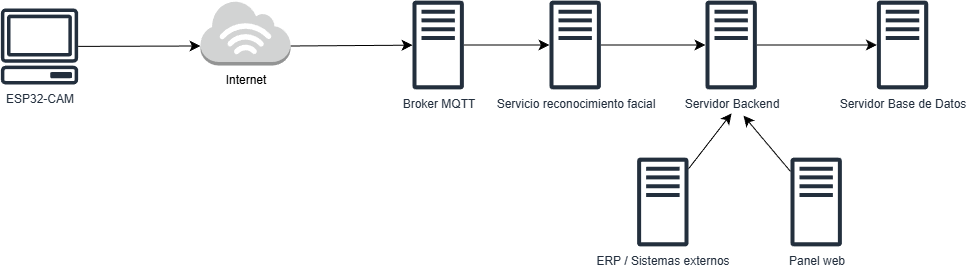
\includegraphics[width=\linewidth]{Imagenes/arqui2.drawio.png}
  \caption{Arquitectura física.}
  \label{fig:arq_fisica}
\end{figure}

\subsection{Arquitectura lógica}
Mientras que la arquitectura física muestra dónde corre cada servicio, la arquitectura lógica de la Fig.~\ref{fig:arq_logica} muestra cómo se organizan los módulos de software dentro de esos servicios y cómo se relacionan entre sí. En el lado del dispositivo, el ESP32-CAM agrupa cuatro módulos: la captura de imágenes (cámara OV2640), la lectura de huella (lector AS608 vía UART), el almacenamiento local en LittleFS (usuarios, turnos, asignaciones y asistencias en formato JSON) y el servidor web embebido que sirve la interfaz de configuración. Estos cuatro módulos no son independientes entre sí: por ejemplo, una marcación capturada por la cámara o el lector se guarda primero en LittleFS y solo después se intenta enviar al backend, lo que permite que el dispositivo siga funcionando aunque no haya conexión.

Del lado del servidor, el backend se organiza en blueprints de Flask (uno por dominio: personas, turnos, asistencias, dispositivos, ERP, etc.), cada uno con acceso a la base de datos PostgreSQL y, cuando corresponde, al servicio de reconocimiento facial. La comunicación entre el dispositivo y el backend ocurre por dos canales según el tipo de mensaje: MQTT para eventos de bajo volumen (heartbeats, comandos, resultados de enrolamiento) y HTTP para el envío de imágenes y la sincronización de datos. Esta separación de canales es la que permite que el dispositivo opere de forma autónoma cuando no hay red, almacene localmente lo que no pudo enviar, y sincronice todo una vez que la conexión se restablece.

\begin{figure}[H]
  \centering
  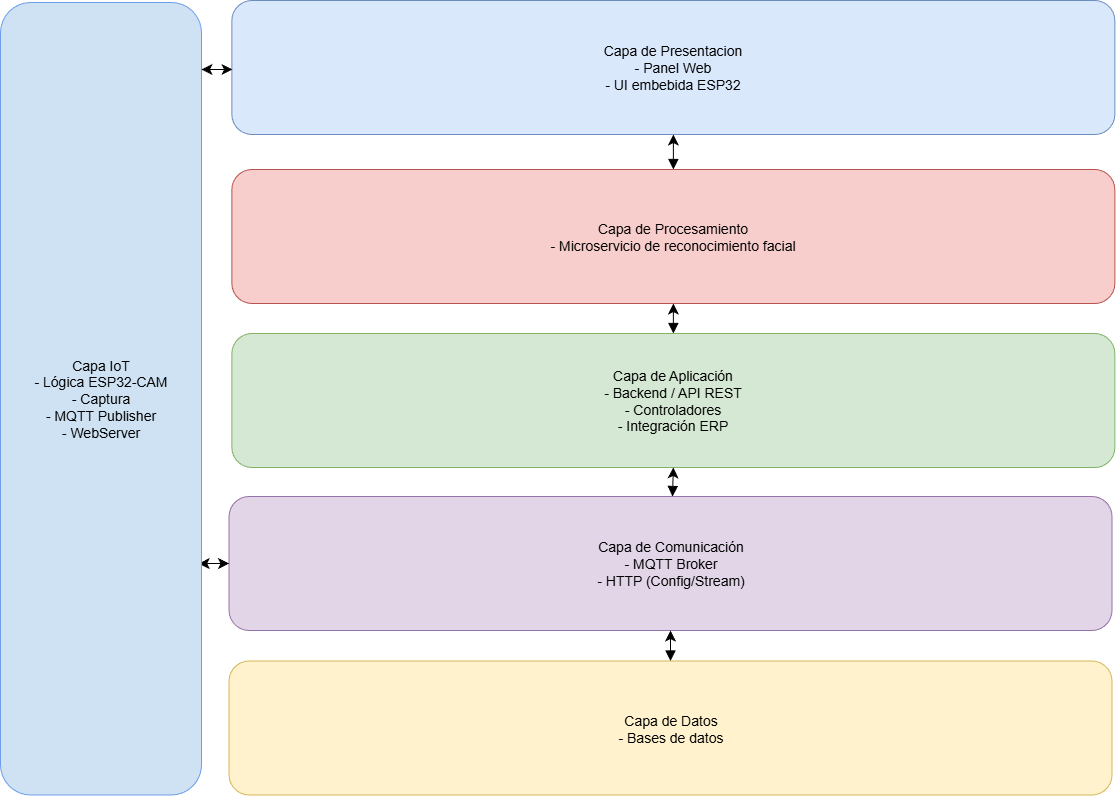
\includegraphics[width=.75\linewidth]{Imagenes/arquilogica.png}
  \caption{Arquitectura lógica.}
  \label{fig:arq_logica}
\end{figure}

La Fig.~\ref{fig:componentes_esp32} detalla, a nivel de hardware y firmware, los mismos cuatro módulos del ESP32-CAM descritos en la arquitectura lógica. En la capa de hardware se distinguen el microcontrolador ESP32, la cámara OV2640 (conectada por el bus paralelo DVP), el lector de huellas AS608 (conectado por UART) y el sensor PIR que activa la captura solo ante presencia detectada. En la capa de firmware, el servidor web embebido y el cliente MQTT comparten el acceso al sistema de archivos LittleFS, mientras que la máquina de estados central coordina cuándo se invoca cada módulo de captura biométrica según si el dispositivo está en modo de registro o de marcaje. Esta vista complementa a la Fig.~\ref{fig:arq_logica}, mostrando con qué pines y protocolos concretos se implementa cada bloque lógico.

\begin{figure}[H]
  \centering
  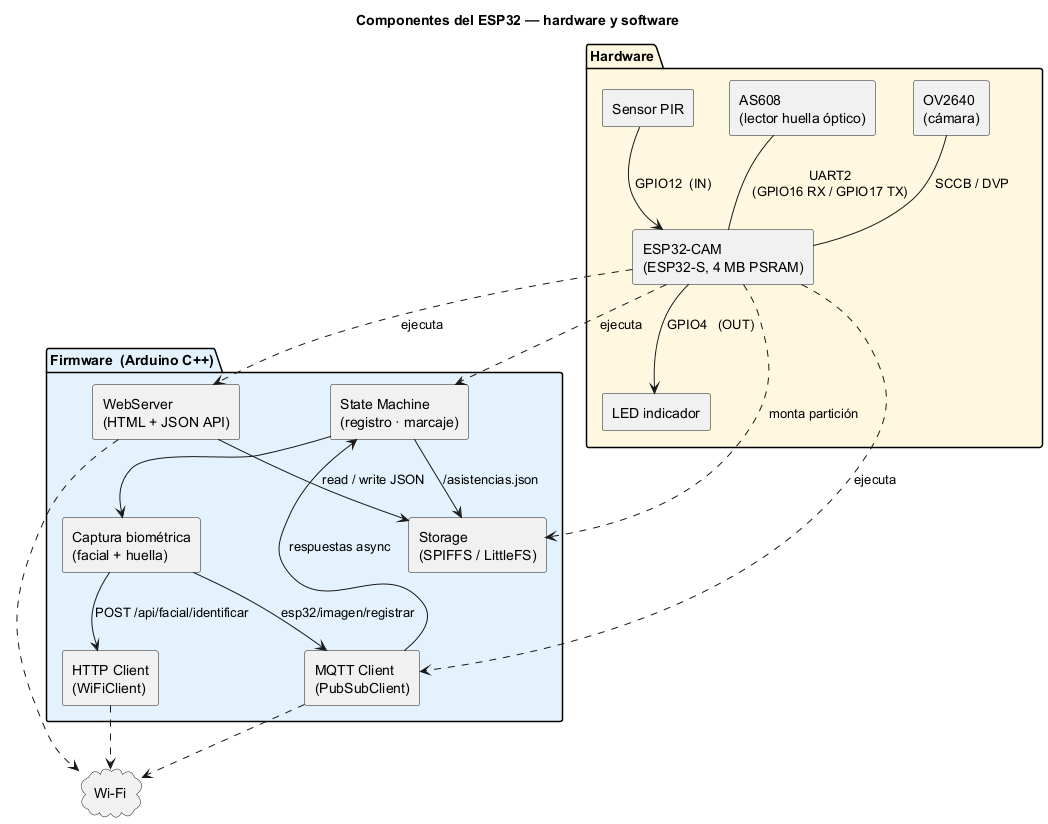
\includegraphics[width=\linewidth]{diagrams/componentes_esp32.png}
  \caption{Componentes del ESP32-CAM: hardware y firmware.}
  \label{fig:componentes_esp32}
\end{figure}

\section{Implementación}

En este apartado se procederá a explicar cómo se llevaron a cabo las iteraciones planteadas en el capítulo 3.1.

%% ============================================================
%% ITERACIÓN 1: Diseño y planificación inicial
%% ============================================================
\subsection{Iteración 1: Integración de hardware y servidor embebido}

La primera iteración corresponde al diseño conceptual del sistema y a la preparación del entorno de desarrollo, incluyendo la integración inicial del hardware biométrico seleccionado. Esta etapa establece la base funcional sobre la cual se construirán las iteraciones posteriores.

\subsubsection{Análisis}

En esta iteración se definieron los requisitos mínimos para validar la viabilidad técnica del sistema, analizando los componentes del hardware y las funcionalidades necesarias para las iteraciones siguientes.

El análisis se centró en tres ejes principales:

\begin{itemize}
    \item \textbf{Definición de funcionalidades mínimas (MVP)}:  
    Se identificaron las capacidades básicas que el dispositivo debía cumplir desde el inicio: capturar imágenes desde la cámara integrada, leer huellas dactilares mediante el sensor AS608, montar un servidor HTTP local con páginas HTML embebidas y operar de forma autónoma mediante Wi-Fi. Estas funciones representan la base operativa sobre la cual se desarrollarán características más avanzadas como turnos, sincronización y gestión de usuarios.

    \item \textbf{Identificación de limitaciones técnicas}:  
    Se revisaron las restricciones tecnológicas del ESP32-CAM, como la limitada memoria RAM disponible (~520 KB), el uso compartido del bus de cámara con los pines GPIO, la ausencia de pines GPIO libres -lo que forzó el uso de los pines GPIO14 (RX) y GPIO15 (TX) para la comunicación UART con el lector de huellas- y la necesidad de un manejo eficiente de cadenas HTML grandes en memoria. También se identificó que el flash LED integrado consume corriente significativa (~250 mA), requiriendo protección mediante PWM para evitar caídas de tensión durante la captura.

    \item \textbf{Estrategia de operación autónoma}:  
    Dado que uno de los requisitos fundamentales del sistema es la autonomía, se analizó la necesidad de montar un servidor web local. En caso de no contar con Wi-Fi configurada, el dispositivo debe activar automáticamente un modo Access Point (AP) con SSID ESP32-ASISTENCIA, permitiendo al administrador conectarse directamente para configurar la red y registrar usuarios sin dependencia de internet. Esto reduce riesgos y asegura la continuidad operacional del dispositivo.
\end{itemize}

Como resultado del análisis, se establecieron los criterios de diseño que guiarían el desarrollo de esta iteración: simplicidad, bajo consumo de recursos, modularidad de componentes y autonomía operativa.

\subsubsection{Diseño}

En esta iteración se elaboraron los primeros elementos arquitectónicos del sistema:

\begin{itemize}
    \item \textbf{Arquitectura física}, representando los componentes utilizados y su interconexión, la cual se puede revisar en la Fig.~\ref{fig:arq_fisica} de la sección 4.1.1.

    \item \textbf{Arquitectura lógica}, definiendo los módulos internos del firmware tales como captura de imágenes, lectura de huella, almacenamiento y conectividad, la cual se puede revisar en la Fig.~\ref{fig:arq_logica} de la sección 4.1.2.

    \item \textbf{Mockups iniciales} de la interfaz embebida del ESP32-CAM, incluyendo:

    \begin{itemize}
        \item Menú principal.
        \begin{figure}[H]
            \centering
            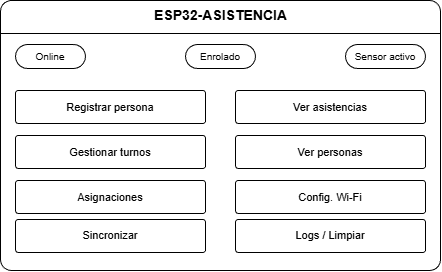
\includegraphics[width=.8\linewidth]{Imagenes/mockup_menu.png}
            \caption{Mockup menú principal en el ESP32-CAM.}
            \label{fig:mockup_menu}
        \end{figure}
        Wireframe inicial de la vista /: agrupa los indicadores de estado del dispositivo (conectividad, enrolamiento, sensor PIR) en la parte superior, y los accesos a cada módulo del sistema (registro, asistencias, turnos, personas, asignaciones, configuración Wi-Fi, sincronización y logs) como botones de navegación.

        \item Panel de configuración de Wi-Fi.
        \begin{figure}[H]
            \centering
            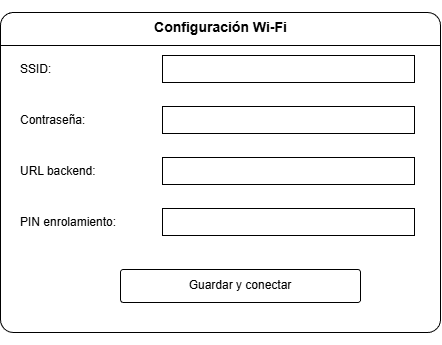
\includegraphics[width=.6\linewidth]{Imagenes/mockup_wifi.png}
            \caption{Mockup panel de configuración Wi-Fi.}
            \label{fig:mockup_wifi}
        \end{figure}
        Wireframe de la vista /wifi-setup: formulario con los cuatro campos que se persisten en wifi.json (SSID, contraseña de red, URL del backend y PIN de enrolamiento), accesible también desde el modo Access Point cuando el dispositivo no tiene credenciales configuradas.

        \item Vista de registro de usuario.
        \begin{figure}[H]
            \centering
            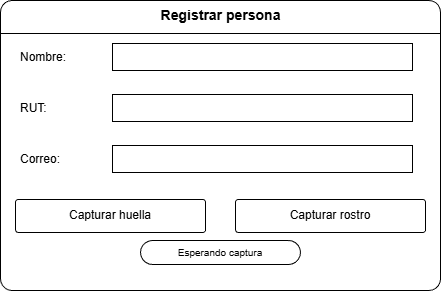
\includegraphics[width=.7\linewidth]{Imagenes/mockup_registro.png}
            \caption{Mockup registro de usuario en el ESP32-CAM.}
            \label{fig:mockup_registro}
        \end{figure}
        Wireframe de la vista /register: formulario de datos básicos (nombre, RUT, correo) seguido de los dos botones de captura biométrica, con un indicador de estado del proceso de enrolamiento (huella y rostro).

        \item Vista de usuarios almacenados localmente.
        \begin{figure}[H]
            \centering
            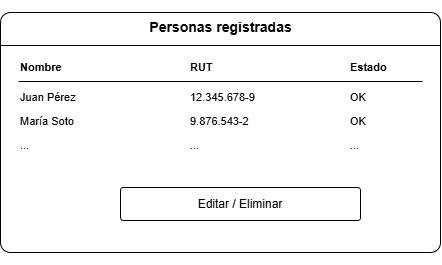
\includegraphics[width=.6\linewidth]{Imagenes/mockup_personas.png}
            \caption{Mockup de usuarios almacenados en el ESP32-CAM.}
            \label{fig:mockup_usuarios}
        \end{figure}
        Wireframe de la vista /personas: listado tabular de las personas registradas leídas desde personas.json, con acciones de edición y eliminación por fila.

        \item Vista de turnos almacenados localmente.
        \begin{figure}[H]
            \centering
            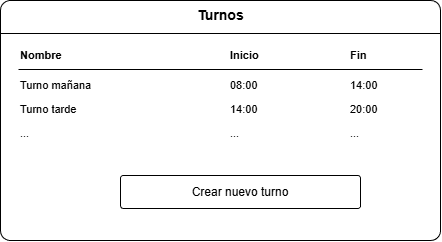
\includegraphics[width=.6\linewidth]{Imagenes/mockup_turnos.png}
            \caption{Mockup de visualización de turnos en el ESP32-CAM.}
            \label{fig:mockup_turnos}
        \end{figure}
        Wireframe de la vista /turnos: listado de los turnos almacenados en turnos.json, con el botón de acceso a la creación de un nuevo turno.

        \item Vista de crear turnos.
        \begin{figure}[H]
            \centering
            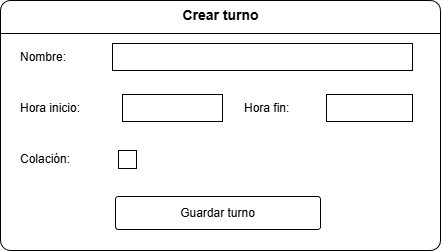
\includegraphics[width=.6\linewidth]{Imagenes/mockup_crear_turno.png}
            \caption{Mockup de creación de turnos en el ESP32-CAM.}
            \label{fig:mockup_crear_turnos}
        \end{figure}
        Wireframe de la vista /gestion: formulario para definir nombre, horario de inicio y fin, y la casilla opcional de colación que habilita los campos colacion\_inicio/colacion\_fin descritos en el Capítulo 4.

        \item Vista de asignación de turnos.
        \begin{figure}[H]
            \centering
            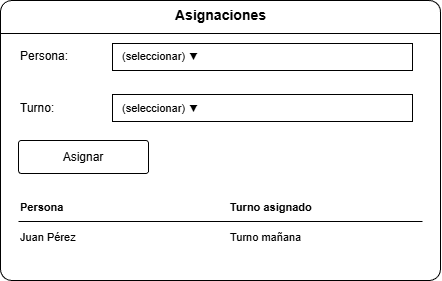
\includegraphics[width=.6\linewidth]{Imagenes/mockup_asignacion.png}
            \caption{Mockup de asignación de turnos en el ESP32-CAM.}
            \label{fig:mockup_asignacion}
        \end{figure}
        Wireframe de la vista /asignaciones: selección de persona y turno mediante listas desplegables, seguida del listado de asignaciones vigentes ya registradas.
    \end{itemize}

    \item \textbf{Diseño del flujo operacional}: a nivel conceptual, se planteó que el dispositivo debía capturar la huella o el rostro y luego evaluar si tenía conectividad disponible. Con conexión, la marcación se enviaría de inmediato al servidor; sin ella, se guardaría localmente para sincronizarse más adelante, cuando la red se restableciera. En ambos casos, la validación final (si la huella o el rostro corresponden a una persona registrada) ocurriría en el servidor, que respondería con un resultado de éxito o de error. El detalle de cómo se implementó cada uno de estos pasos, una vez que todos los componentes involucrados (enrolamiento, reconocimiento facial, sincronización diferida e integración ERP) estuvieron construidos, se presenta de forma consolidada al cierre del desarrollo, en la Sección~\ref{sec:flujo_operacional_consolidado}.
\end{itemize}

Estos elementos permiten visualizar el flujo básico del dispositivo antes de incorporar funcionalidades adicionales como turnos, sincronización o panel web backend, los cuales se desarrollarán en iteraciones posteriores.

\subsubsection{Implementación}

En esta etapa se integró tanto el hardware principal del prototipo como el desarrollo de las vistas web embebidas que permiten la interacción del usuario con el dispositivo. Para ello se utilizaron las siguientes librerías:

\begin{itemize}
    \item esp\_camera, utilizada para inicializar y configurar la cámara OV2640 integrada en el ESP32-CAM.
    \item HardwareSerial y Adafruit\_Fingerprint, empleadas para la comunicación UART con el lector biométrico AS608.
    \item WebServer, utilizada para montar un servidor web HTTP en el puerto 80 y atender rutas asociadas a las vistas.
    \item LittleFS y ArduinoJson \cite{arduinojson_docs}, empleadas para almacenamiento persistente en memoria flash y manipulación estructurada de datos JSON.
\end{itemize}

\paragraph{Integración del lector de huellas AS608}

El lector biométrico AS608 fue conectado directamente al ESP32-CAM mediante la interfaz UART secundaria (HardwareSerial 2), utilizando los pines GPIO14 (RX) y GPIO15 (TX). Esta conexión, que emplea pines distintos a los documentados inicialmente, fue forzada por la escasez de GPIO libres tras la asignación del bus de cámara. La velocidad de comunicación se estableció en 57600 baudios, y la librería Adafruit\_Fingerprint se vincula a dicho puerto serial. La Figura~\ref{fig:conexioneshuella} presenta la conexión física entre ambos dispositivos.

\begin{figure}[H]
    \centering
    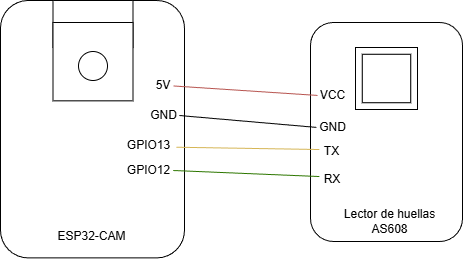
\includegraphics[width=.8\linewidth]{Imagenes/conexiones.png}
    \caption{Conexiones entre el ESP32-CAM y el lector de huellas AS608.}
    \label{fig:conexioneshuella}
\end{figure}

Una vez establecida la comunicación, el firmware puede ejecutar operaciones como:

\begin{itemize}
    \item Captura de imagen dactilar.
    \item Conversión de la imagen en una plantilla biométrica.
    \item Almacenamiento del template en un slot interno del sensor (1-127).
    \item Identificación mediante búsqueda de coincidencias en memoria.
\end{itemize}

La inicialización del lector se realiza con finger.begin(57600) sobre el puerto serie secundario, seguida de finger.verifyPassword() para confirmar que el sensor responde correctamente antes de habilitar las operaciones de captura, conversión y búsqueda descritas anteriormente.

\paragraph{Configuración de la cámara y el flash PWM}

La cámara OV2640 se configuró con resolución VGA (640×480) y compresión JPEG con calidad 8 (escala 0-63, donde valores bajos indican mayor calidad). La frecuencia del reloj externo (XCLK) se fijó en 20 MHz. Para evitar el parpadeo visible y las caídas de tensión provocadas por el flash LED durante la captura, se implementó un control PWM a 5 kHz con resolución de 8 bits, aplicando un ciclo de trabajo del 50\% (duty 128 de 255) durante la iluminación. Esto permite encender el flash con brillo suficiente sin sobrecargar la fuente de alimentación del ESP32-CAM.

\paragraph{Calibración del sensor PIR}

Se integró un sensor PIR (Passive Infrared) conectado al GPIO12 configurado con resistencia de pull-down interna. El sensor PIR actúa como detector de presencia: cuando una persona se sitúa frente al dispositivo, el PIR detecta el cambio de radiación infrarroja y activa el modo de captura. El setup incluye una fase de calibración de 3 segundos para estabilizar la lectura del sensor antes de iniciar el bucle principal. La lógica de uso del PIR como control de activación se detalla en la iteración 6.

\paragraph{Montaje del servidor web embebido}

Para habilitar la interacción local con el dispositivo, se implementó un servidor web mediante la librería WebServer en el puerto 80. Este servidor permite entregar páginas HTML, datos JSON y recursos estáticos. Cuando no hay conectividad a una red externa, el ESP32-CAM activa automáticamente un Access Point con SSID ESP32-ASISTENCIA y contraseña Asistencia2026, sirviendo las mismas páginas sin depender de internet.

Las rutas principales del sistema incluyen:

\begin{itemize}
    \item /: Menú principal con indicadores de estado.
    \item /wifi-setup: Configuración de red Wi-Fi y parámetros del backend.
    \item /register: Registro de personas con captura biométrica.
    \item /asistencias: Lista de asistencias almacenadas localmente.
    \item /gestion: Gestión de turnos (creación y administración).
    \item /personas: Visualización de personas registradas.
    \item /asignaciones: Vista para realizar asignaciones de turnos.
    \item /logs: Visualización de logs del sistema.
    \item /turnos: Visualización de turnos creados.
\end{itemize}

Para la implementación del servidor HTTP embebido, se utilizó el módulo WebServer del ESP32. Cada operación del sistema (registro de usuarios, captura de huellas, creación de turnos, asignación de turnos, lectura de asistencias, configuración Wi-Fi, entre otras) fue mapeada a un endpoint específico mediante funciones manejadoras (handler functions), registradas mediante "server.on(ruta, metodo, handler)" para cada una de las rutas listadas anteriormente. Este mecanismo permite encapsular la lógica de cada componente del sistema y mantener una estructura modular del firmware.

\paragraph{Creación de vistas HTML embebidas}

Las vistas fueron desarrolladas como archivos .html independientes almacenados en el sistema de archivos LittleFS del ESP32-CAM, conteniendo HTML, CSS y JavaScript autónomo, sin dependencias de CDN externas. El servidor web embebido las sirve mediante la función servirArchivo(), que lee el archivo solicitado desde LittleFS y lo envía al cliente. Esto garantiza que el ESP32-CAM sirva cada página incluso en modo Access Point sin conexión a internet.

\paragraph{Menú principal}

La Figura~\ref{fig:menu_principal} presenta la vista principal accesible en la ruta /. Desde esta interfaz el usuario puede visualizar el estado del dispositivo (online/offline, sensor activo, enrolado), registrar personas, ver asistencias, gestionar turnos, ver asignaciones, acceder a la configuración de red, sincronizar con el backend y limpiar datos del dispositivo. Con el avance de las iteraciones se agregaron a esta vista los indicadores de estado que se actualizan cada pocos segundos consultando al dispositivo, un bloque para mostrar el PIN de registro que permanece oculto hasta que el usuario decide revelarlo, una zona separada para las acciones de reinicio y borrado total de datos, y la opción de proteger la página con contraseña de administrador cuando se requiere restringir el acceso a esas acciones.

\begin{figure}[H]
    \centering
    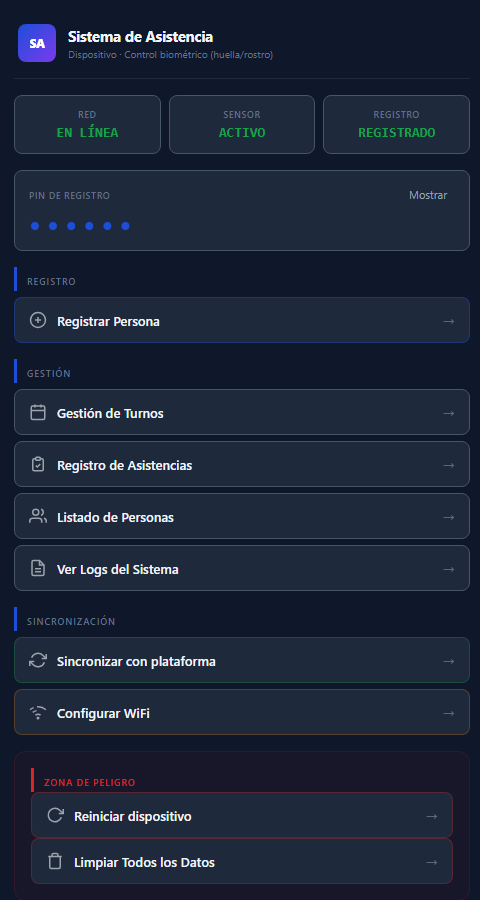
\includegraphics[height=8.5cm,keepaspectratio]{Imagenes/menuimplementado.png}
    \caption{Menú principal del sistema web embebido.}
\label{fig:menu_principal}
\end{figure}

\paragraph{Vista de configuración Wi-Fi}

Mediante la ruta /wifi-setup, el dispositivo proporciona un formulario para actualizar las credenciales de la red local (SSID, contraseña), la URL del backend, la dirección del broker MQTT y el PIN de enrolamiento. Estos valores se persisten en SPIFFS mediante el archivo wifi.json. La Figura~\ref{fig:wifi_config} muestra esta interfaz. Por requerimientos de seguridad identificados en iteraciones posteriores, se agregó a esta vista la opción de forzar conexiones cifradas hacia el backend y el broker MQTT, además de un apartado donde se puede definir o cambiar la contraseña de administrador pidiendo la contraseña actual como confirmación, de modo que no cualquier persona con acceso a la red local pueda modificar la configuración del dispositivo.

\begin{figure}[H]
    \centering
    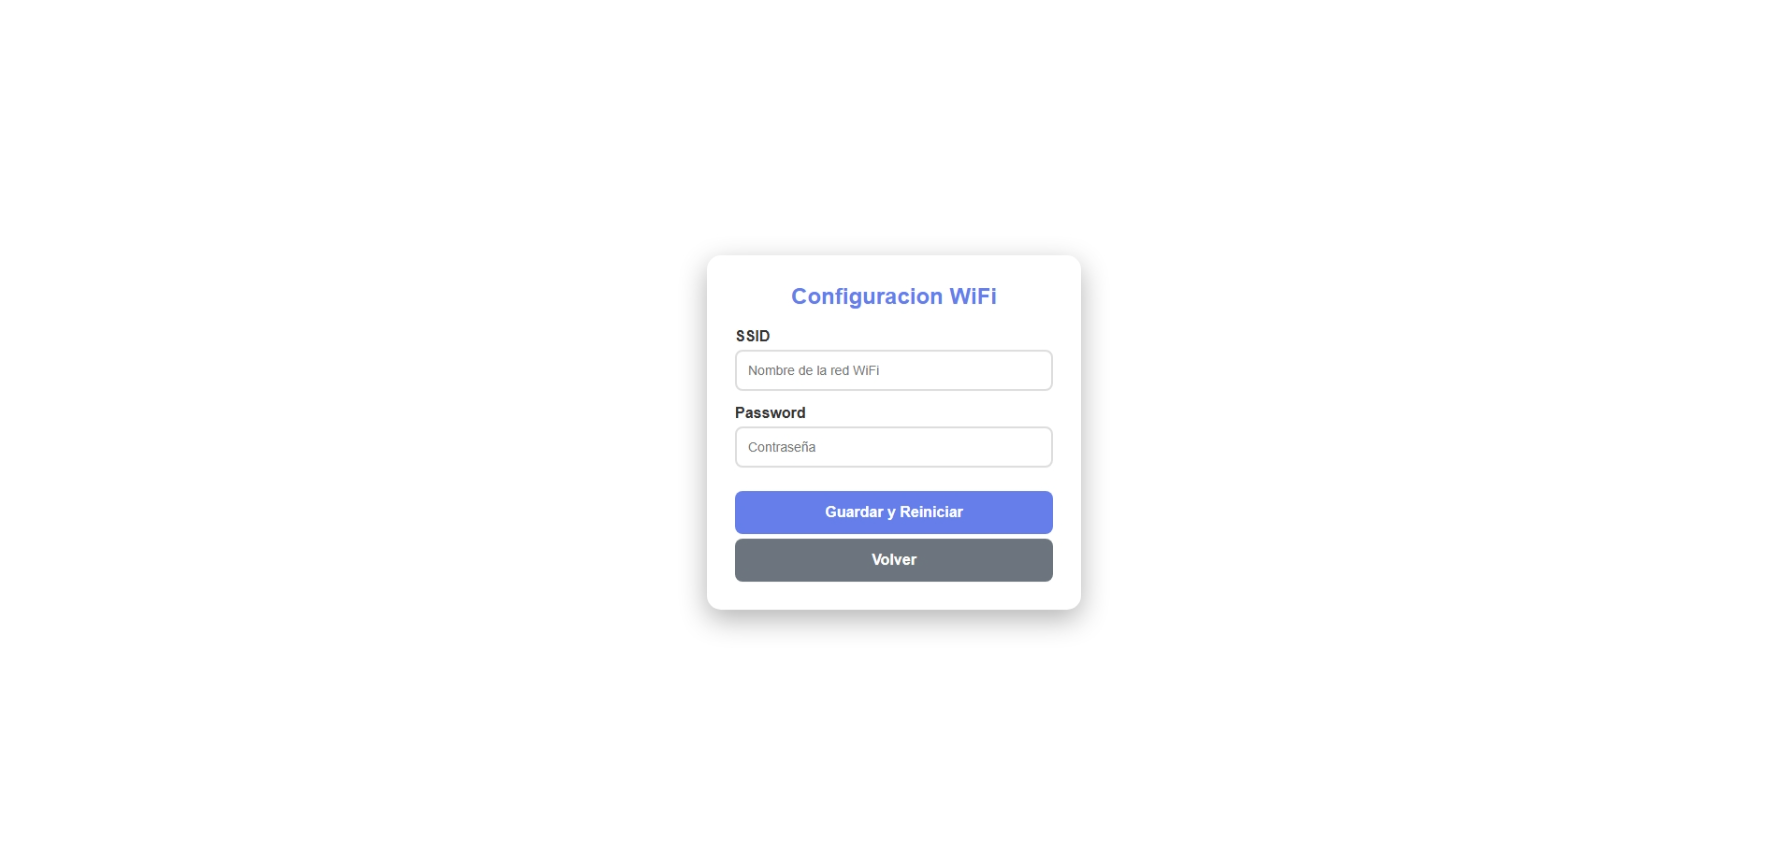
\includegraphics[height=8.5cm,keepaspectratio]{Imagenes/menuwifiimplementado.png}
    \caption{Interfaz de configuración Wi-Fi.}
\label{fig:wifi_config}
\end{figure}

\paragraph{Vista de registro de personas}

La ruta /register despliega una vista que combina un formulario para ingresar el nombre del usuario, RUT y correo electrónico, y muestra indicadores visuales del estado del proceso de enrolamiento (huella, rostro). La Figura~\ref{fig:registro_personas} lo muestra. Se incorporó a esta vista una casilla de consentimiento explícito para el tratamiento de datos biométricos, exigida por las consideraciones éticas y de privacidad descritas en el marco metodológico; mientras no se marque, el botón para iniciar el registro biométrico queda deshabilitado. El flujo se complementó además con un panel que informa el avance del proceso y con una pantalla de captura facial guiada, que muestra cuántas de las tres fotografías necesarias para el reconocimiento facial ya se han tomado.

\begin{figure}[H]
    \centering
    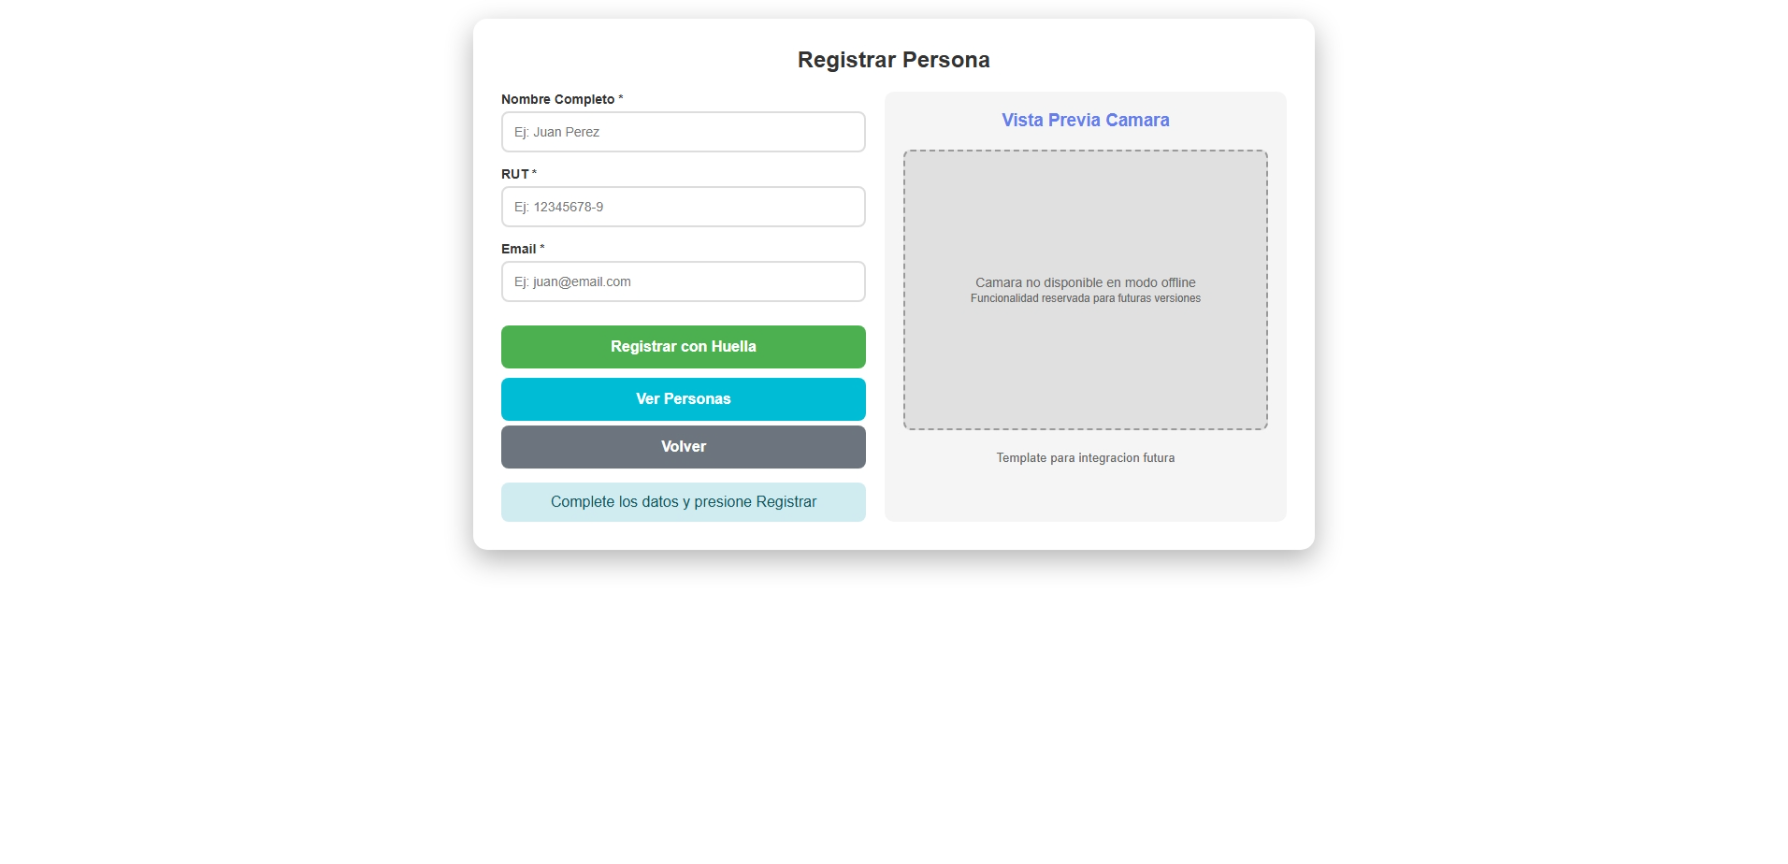
\includegraphics[height=8.5cm,keepaspectratio]{Imagenes/registroimplementado.png}
    \caption{Vista para el registro de personas en el dispositivo.}
\label{fig:registro_personas}
\end{figure}

\paragraph{Vista de asistencias}

Para visualizar registros de asistencia tanto locales como sincronizados, se implementó la vista en la ruta /asistencias. Esta consulta archivos JSON almacenados en LittleFS. La Figura~\ref{fig:vista_asistencias} lo ejemplifica. Cada registro se presenta como una tarjeta diferenciada por color según sea entrada o salida, con el nombre de la persona, la marca de tiempo y su identificador asociado. A la versión inicial, que solo listaba los registros, se le agregaron las opciones de editar o eliminar cada fila, pensadas para que el encargado de turno pueda corregir una marcación errónea, como una doble lectura biométrica, sin necesidad de acceder directamente al backend. También se sumó un contador de registros totales en la parte superior, útil para revisar de un vistazo cuántos datos hay almacenados localmente antes de sincronizar.

\begin{figure}[H]
    \centering
    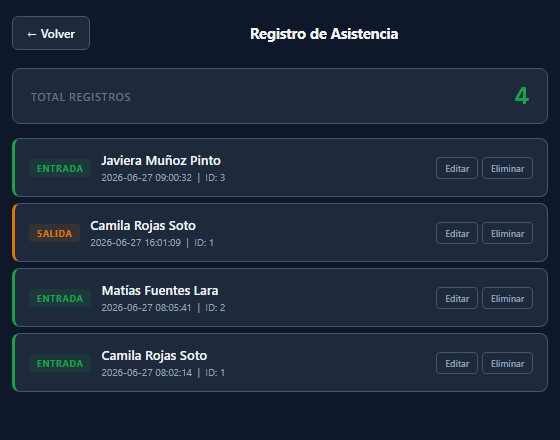
\includegraphics[height=8.5cm,keepaspectratio]{Imagenes/vistaasitenciasimplementado.png}
    \caption{Vista de asistencias locales almacenadas en el dispositivo.}
\label{fig:vista_asistencias}
\end{figure}

\paragraph{Vista de Personas registradas}

Para visualizar las personas registradas, se implementó la vista en la ruta /personas. Esta consulta archivos JSON almacenados en LittleFS y permite editar nombre/correo, actualizar huella o rostro, y eliminar personas. La Figura~\ref{fig:personas_registradas} lo ejemplifica. Las opciones para actualizar la huella o el rostro, y para agregar fotos adicionales, se incorporaron después de notar en las pruebas de campo que volver a registrar a una persona desde cero, borrando y repitiendo todo el proceso, tomaba demasiado tiempo. Con estas opciones se puede corregir solo la huella o el rostro de alguien ya registrado, o sumar fotos para mejorar el reconocimiento facial, sin perder el resto de sus datos ni su historial de asistencia.

\begin{figure}[H]
    \centering
    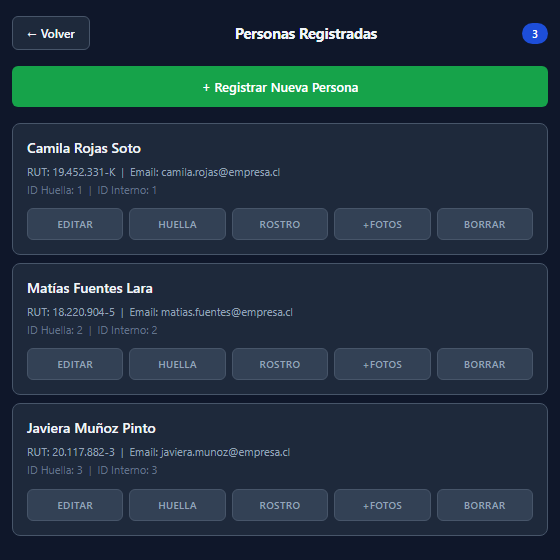
\includegraphics[height=8.5cm,keepaspectratio]{Imagenes/personasregistradasimplementada.png}
    \caption{Vista de personas registradas en el dispositivo.}
\label{fig:personas_registradas}
\end{figure}

\paragraph{Vista de Crear Turnos}

Para la creación de turnos y visualización de los existentes, se implementó la vista en la ruta /gestion, complementada con /turnos. Estas consultan archivos JSON almacenados en LittleFS. La Figura~\ref{fig:gestion_turnos} lo ejemplifica. La vista /gestion funciona como panel resumen, con accesos directos a la gestión de turnos, a las asignaciones y a la sincronización manual con la plataforma. La vista /turnos concentra el formulario para crear un turno nuevo, con nombre, hora de inicio y fin, y un selector de días de la semana, junto con el listado editable de los turnos ya creados. Esta separación entre resumen y edición se introdujo para que las modificaciones no ocurran por accidente desde la pantalla que se usa con más frecuencia.

\begin{figure}[H]
    \centering
    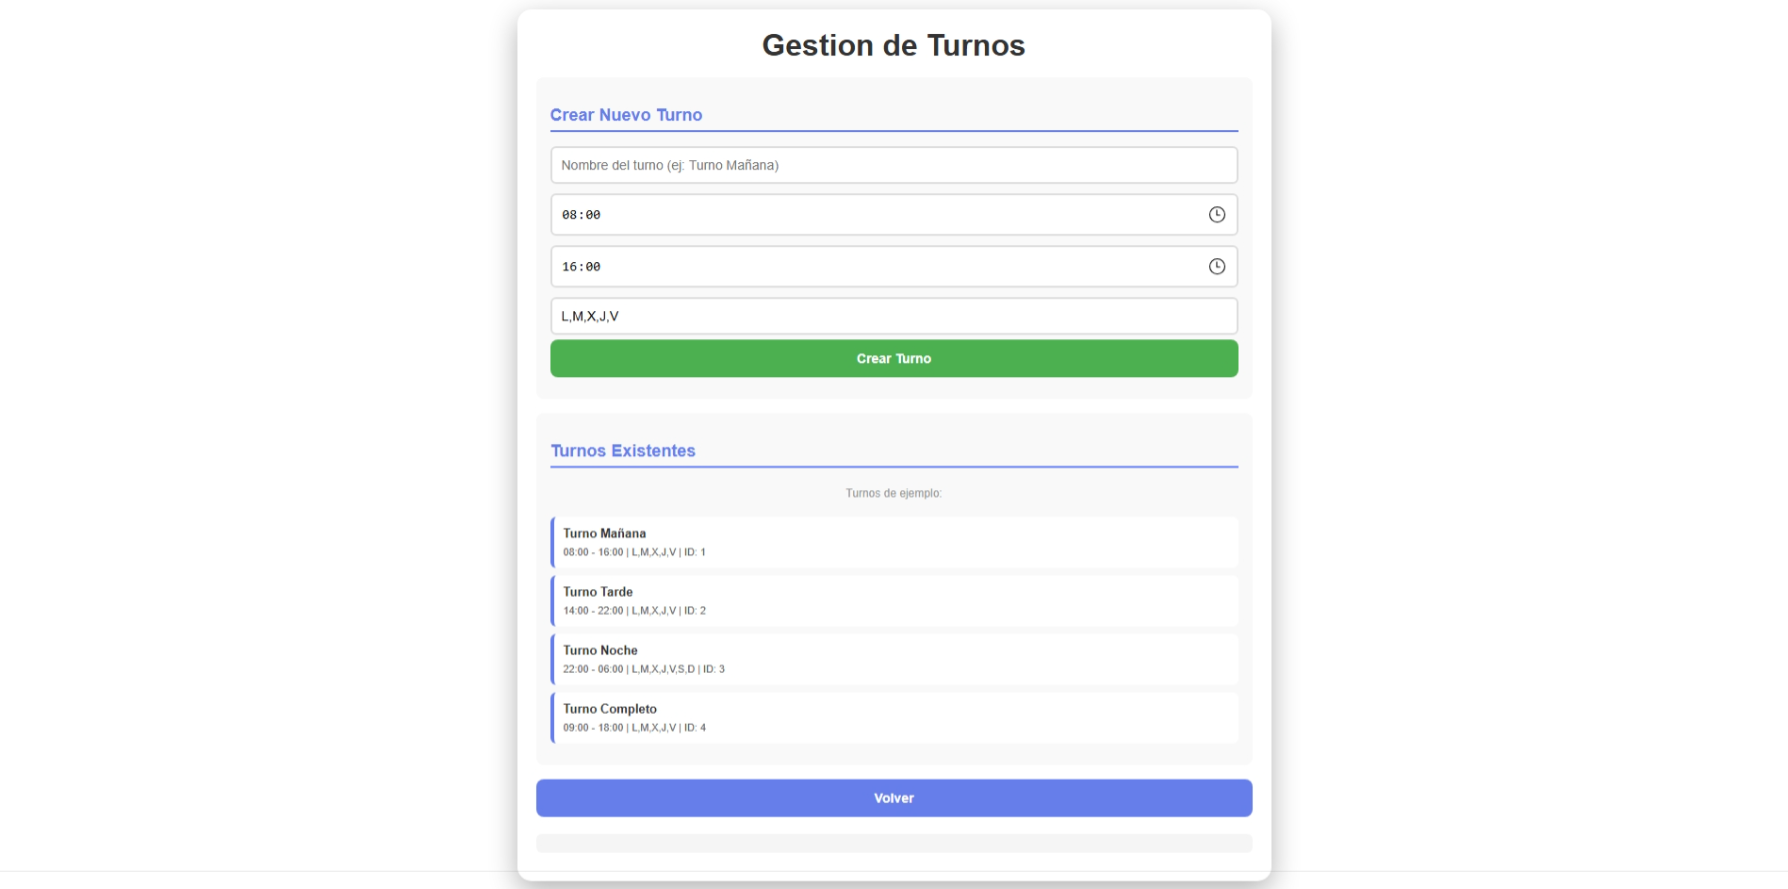
\includegraphics[height=8.5cm,keepaspectratio]{Imagenes/creacionturnos.png}
    \caption{Vista de gestión y creación de turnos en el dispositivo.}
\label{fig:gestion_turnos}
\end{figure}

\paragraph{Vista de asignación de turnos}

Para visualizar las asignaciones de turnos y realizar la acción de asignar un turno a una persona, se implementó la vista en la ruta /asignaciones. La Figura~\ref{fig:asignacion_turnos} lo ejemplifica. El formulario superior permite elegir una persona y un turno ya creados desde listas desplegables, evitando que el usuario tenga que recordar o escribir identificadores internos. El listado de asignaciones actuales muestra el nombre de la persona y del turno en lugar de solo sus identificadores, e incluye una opción para quitar una asignación, agregada después de notar que reasignar turnos por cambios de horario del personal era algo que ocurría seguido durante el uso del prototipo.

\begin{figure}[H]
    \centering
    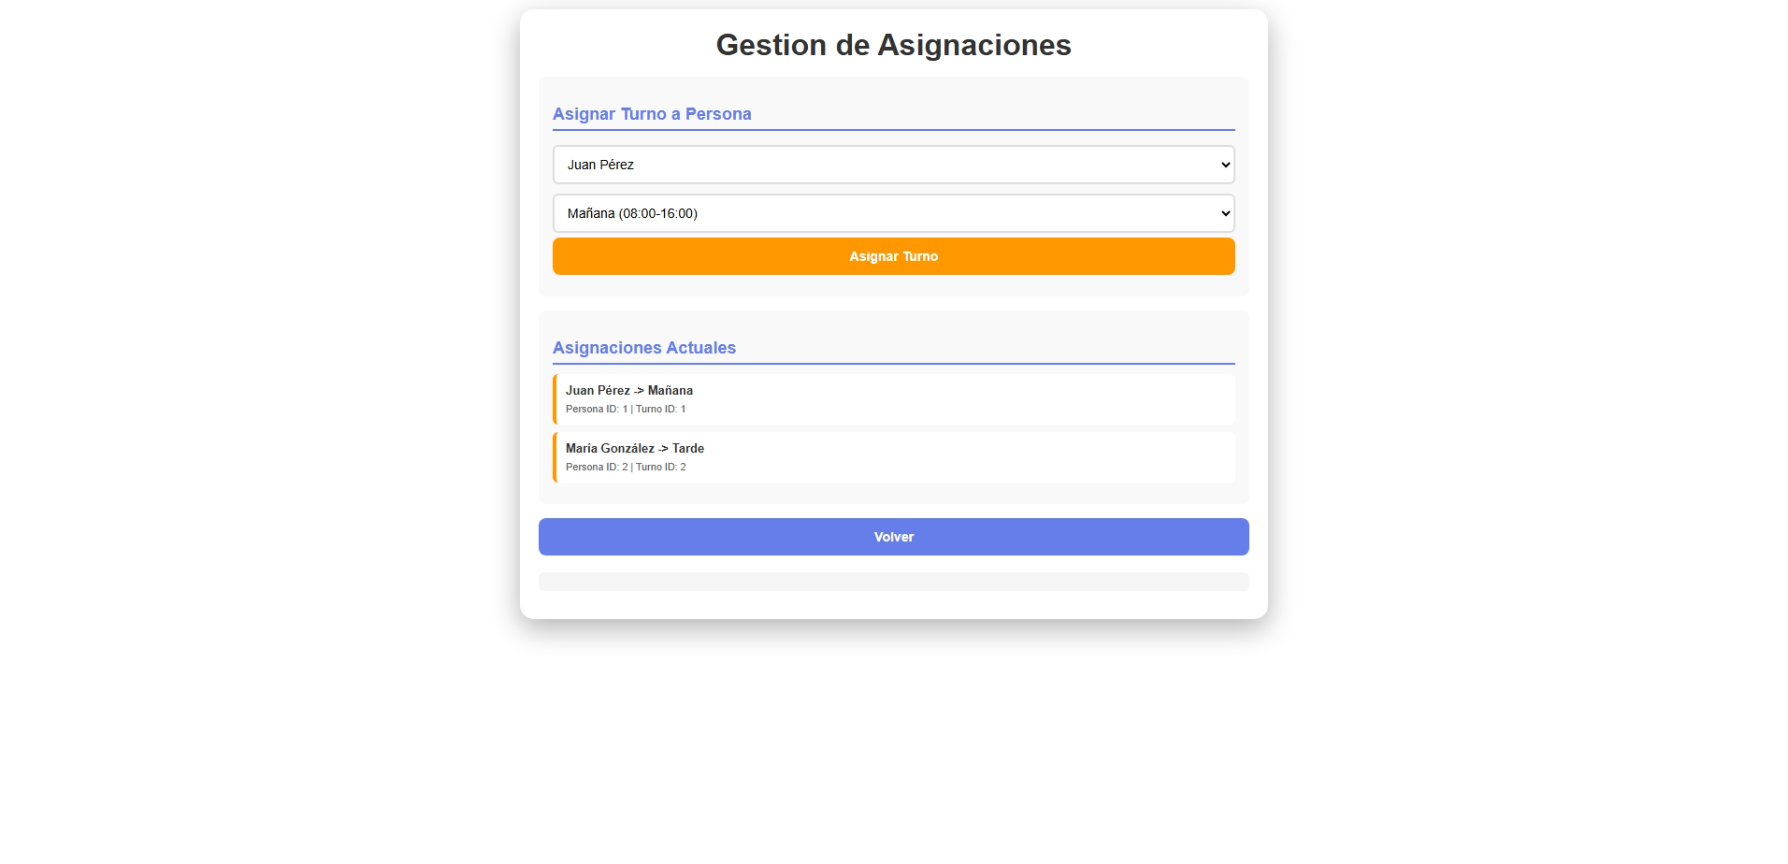
\includegraphics[height=8.5cm,keepaspectratio]{Imagenes/asignacionturnoimplementacion.png}
    \caption{Vista de gestión de asignaciones en el dispositivo.}
\label{fig:asignacion_turnos}
\end{figure}

\subsubsection{Pruebas}

Para validar el funcionamiento del prototipo y comprobar la correcta integración entre los distintos módulos del sistema, se diseñaron pruebas de integración enfocadas exclusivamente en los componentes implementados durante esta iteración:

\begin{itemize}
    \item \textbf{Prueba de captura de imágenes}: Verificar que la cámara OV2640 capture imágenes JPEG de forma continua y estable, sin corrupción de frames ni errores de inicialización del sensor. Se espera que la función esp\_camera\_fb\_get() retorne buffers consistentes tras cada llamada.

    \item \textbf{Prueba de comunicación UART con AS608}: Verificar que el lector biométrico responda correctamente al comando de verificación de contraseña (finger.verifyPassword()) y que la comunicación serie a 57600 baudios se establezca sin pérdida de paquetes. Se espera confirmación de conexión en menos de 1 segundo tras el inicio.

    \item \textbf{Prueba de lectura biométrica}: Verificar que el AS608 pueda capturar una imagen dactilar (finger.getImage()), convertirla a plantilla (finger.image2Tz()) y almacenarla en un slot del sensor (finger.storeModel()). Se espera que el proceso completo tome menos de 2 segundos.

    \item \textbf{Prueba de acceso vía AP}: Verificar que al iniciar sin credenciales Wi-Fi configuradas, el ESP32-CAM active el Access Point ESP32-ASISTENCIA y que las páginas HTML sean accesibles desde un navegador conectado a la IP 192.168.4.1. Se espera que todas las rutas definidas respondan con código HTTP 200.

    \item \textbf{Prueba de carga de vistas vía Wi-Fi externa}: Verificar que al conectar el dispositivo a una red Wi-Fi configurada, las mismas vistas se carguen correctamente a través de la IP asignada por el router, manteniendo estilos, scripts y funcionalidad.
\end{itemize}

\subsubsection{Refinamientos posteriores}

Durante el desarrollo de las iteraciones siguientes surgieron dos problemas asociados a la base construida en esta etapa, los cuales fueron corregidos durante el mismo ciclo de implementación.

El primero se presentó al combinar las funcionalidades de conectividad y enrolamiento: un dispositivo podía encontrarse conectado a internet sin contar aún con una persona enrolada, o bien tener una persona enrolada pero haber perdido la conexión de red. En ambos casos, el firmware intentaba ejecutar la sincronización o el reconocimiento facial de igual forma, lo que provocaba fallos sin generar un mensaje de error claro para el usuario. Para resolver esta situación, se implementó una función de validación que verifica simultáneamente ambas condiciones antes de permitir cualquier operación dependiente del backend, evitando así que el dispositivo ejecute procesos que se sabe resultarán en error.

El segundo ajuste estuvo relacionado con la calidad de las imágenes utilizadas para el reconocimiento facial. Las capturas estándar de la cámara se almacenaban con un nivel de compresión orientado a vistas previas rápidas, el cual resultaba insuficiente para generar un embedding facial de calidad adecuada, debido a la pérdida de detalle en los rasgos del rostro. Por este motivo, se diferenció el proceso de captura correspondiente al registro biométrico, incrementando temporalmente la resolución del sensor exclusivamente para la fotografía de referencia, y restableciéndola a su configuración estándar una vez completada la captura, sin afectar el resto de las imágenes procesadas por el sistema.

%% ============================================================
%% ITERACIÓN 2: Almacenamiento local y modo offline
%% ============================================================

\subsection{Iteración 2: Almacenamiento local y modo offline}

La segunda iteración se centra en habilitar el funcionamiento autónomo del dispositivo sin conexión a internet, integrando un sistema de almacenamiento persistente basado en LittleFS (sucesor moderno de SPIFFS para ESP32) y los mecanismos de captura biométrica offline. Esta etapa materializa lo definido en el apartado 3.1.2 del capítulo anterior.

\subsubsection{Análisis}

Para el correcto funcionamiento offline del prototipo se identificaron los siguientes requerimientos:

\begin{itemize}
    \item Almacenar localmente los datos de usuarios, turnos, asignaciones y asistencias en formato JSON.
    \item Permitir el registro de marcaciones aun cuando no exista conectividad externa, tanto por huella (offline total) como con validación de turnos locales.
    \item Garantizar persistencia de la información tras reinicios del ESP32-CAM o cortes de energía.
    \item Habilitar la gestión completa del sistema mediante una interfaz web embebida accesible vía Access Point.
    \item Mantener compatibilidad con la futura sincronización automática en modo online, marcando cada registro con un campo sincronizado (booleano) para su posterior envío al backend.
\end{itemize}

Para cumplir estos requisitos se seleccionó el sistema de archivos LittleFS y el formato JSON debido a su bajo peso, facilidad de manipulación mediante la librería ArduinoJson y compatibilidad con las capacidades del ESP32-CAM (4 MB de flash, de los cuales aproximadamente 1.5 MB están disponibles para LittleFS). Adicionalmente, se definió un archivo de configuración, wifi.json, destinado a almacenar credenciales Wi-Fi, URL del backend, dirección del broker MQTT y PIN de enrolamiento.

\subsubsection{Diseño}

Considerando la arquitectura establecida, se diseñaron las siguientes estructuras de almacenamiento en formato JSON:

\begin{itemize}
    \item \textbf{personas.json}: Arreglo de objetos con campos id, nombre, rut, email, huella\_id, fecha\_registro, sincronizado.
    \item \textbf{turnos.json}: Arreglo de objetos con campos id, backend\_id, nombre, inicio, fin, dias, sincronizado.
    \item \textbf{asignaciones.json}: Arreglo de objetos con campos persona\_id, turno\_id, backend\_id, fecha\_asignacion, sincronizado.
    \item \textbf{asistencias.json}: Arreglo de objetos con campos persona\_id, nombre, tipo (entrada/salida), metodo (huella\_offline, facial, etc.), timestamp, sincronizado.
    \item \textbf{wifi.json}: Objeto con campos ssid, pass, backend, mqtt, pin (para enrolamiento del dispositivo).
    \item \textbf{erp-config.json}: Arreglo con configuraciones de integraciones ERP, sincronizado desde el backend cuando hay conectividad.
\end{itemize}

El campo sincronizado (booleano) en cada entidad actúa como bandera para el proceso de sincronización diferida: cuando el dispositivo recupera conectividad, itera sobre los registros con sincronizado = false y los envía al backend. Una vez confirmada la recepción, se marca sincronizado = true.

\subsubsection{Implementación}

En esta iteración se integraron las librerías LittleFS, ArduinoJson, HardwareSerial y Adafruit\_Fingerprint. Las dos primeras permiten gestionar archivos JSON alojados en la memoria flash del ESP32-CAM, mientras que las dos últimas habilitan la comunicación UART con el lector biométrico AS608 para el registro y verificación de huellas digitales.

\paragraph{Inicialización del sistema de archivos y persistencia}

El primer componente de la implementación consiste en montar LittleFS mediante LittleFS.begin(true) y verificar la existencia de los archivos necesarios. En caso de no existir, el sistema los crea con una estructura inicial vacía (arreglo [] para las colecciones, objeto con valores por defecto para wifi.json), asegurando que el dispositivo pueda operar incluso tras un primer arranque sin configuración previa.

Se implementaron dos funciones genéricas para la manipulación de archivos JSON:

\begin{itemize}
    \item loadArray(const char* path, DynamicJsonDocument\& doc): Abre un archivo, deserializa su contenido como JsonArray y lo retorna. Si el archivo no existe o está corrupto, retorna un arreglo vacío.
    \item saveArray(const char* path, DynamicJsonDocument\& doc): Serializa el documento JSON y lo escribe en el archivo correspondiente, sobrescribiendo el contenido anterior.
\end{itemize}

Estas funciones encapsulan toda la lógica de persistencia del sistema y son reutilizadas por todos los módulos que necesiten leer o escribir datos.

El tamaño de cada DynamicJsonDocument se dimensionó según el volumen esperado de datos de cada archivo, aunque varía según la función que lo utiliza: asignaciones.json utiliza típicamente 1024~bytes, personas.json y turnos.json se manejan con buffers de entre 2048 y 8192~bytes dependiendo del contexto (lectura local, sincronización o registro), y asistencias.json utiliza 32768~bytes. Adicionalmente, en la función procesarAsistencia() se incorporó una validación sobre el retorno de createNestedObject(): si el objeto retornado es nulo (indicando desbordamiento del documento), se registra una advertencia en el log del sistema, permitiendo detectar tempranamente cuellos de botella de memoria sin comprometer la integridad del archivo JSON. El dimensionamiento de este buffer y la estrategia adoptada para sostener el volumen de registros exigido en los objetivos del proyecto se detallan en el apartado de refinamientos posteriores de esta iteración.

\paragraph{Registro de usuarios con huella digital}

El registro de usuarios se implementó mediante un flujo que combina la captura biométrica gestionada por el lector AS608 con el almacenamiento en personas.json. El lector administra internamente modelos de huellas mediante \textit{slots} numerados del 1 al 127. Por ello, antes del enrolamiento es necesario identificar un slot disponible dentro del sensor. La función encontrarSlotLibre() recorre el arreglo de personas, determina el ID de huella más alto registrado y retorna el siguiente disponible.

Una vez encontrado un slot, se ejecuta el proceso de enrolamiento en dos fases:

\begin{enumerate}
    \item \textbf{Primera captura} (ESTADO\_ESPERANDO\_HUELLA\_REGISTRO): El sistema espera que el usuario coloque el dedo. Al detectar una imagen válida, la convierte a plantilla en el buffer 1 y transiciona a ESTADO\_ESPERANDO\_SOLTAR\_DEDO.
    \item \textbf{Espera y segunda captura} (ESTADO\_REGISTRO\_SEGUNDA\_HUELLA): Una vez que el sensor detecta que el dedo fue retirado (FINGERPRINT\_NOFINGER), el sistema solicita una segunda captura del mismo dedo. Al obtenerla, convierte a plantilla en el buffer 2, crea el modelo combinado (finger.createModel()) y lo almacena en el slot correspondiente (finger.storeModel()).
\end{enumerate}

Luego del enrolamiento exitoso, se almacena un nuevo objeto dentro de personas.json con un identificador único (generado localmente con prefijo local- o provisto por el backend si hay conectividad), el nombre, RUT, correo electrónico y el slot asignado. La etapa de captura de huella aquí descrita corresponde a los primeros estados de la máquina de estados del registro biométrico completo, presentada más adelante en la Figura~\ref{fig:maquina_estados_esp32} (sección 4.3.4), una vez introducido el envío de la foto de referencia al backend por HTTP.

\paragraph{Registro de asistencia en modo offline}

El registro de asistencia se realiza completamente en el dispositivo, sin necesidad de conexión externa. El flujo implementado consiste en:

\begin{enumerate}
    \item Capturar una huella mediante el lector AS608 (finger.getImage()).
    \item Convertir la imagen a plantilla (finger.image2Tz()) y ejecutar una búsqueda biométrica (finger.fingerSearch()) que retorna el fingerID del slot coincidente.
    \item Identificar al usuario asociado mediante el campo huella\_id en personas.json con la función buscarPersonaPorHuella().
    \item Verificar que el usuario cuente con un turno asignado consultando asignaciones.json mediante turnoActivo(). Si no tiene turno, el sistema rechaza la marcación.
    \item Determinar el tipo de evento (entrada/salida) alternando automáticamente respecto al último registro de la persona en asistencias.json.
    \item Generar un nuevo registro con sincronizado = false (salvo que se logre enviar al backend en ese momento).
\end{enumerate}

El manejador handleMarcarAsistencia() expone esta funcionalidad a través de la interfaz web, permitiendo también marcaciones manuales. El escaneo automático continuo se controla mediante intervalos configurables: 2 segundos entre verificaciones de huella y 6 segundos entre verificaciones faciales.

\paragraph{Gestión de turnos y asignaciones}

Además del registro de asistencias, el sistema permite crear turnos (handleCreateTurn()) y asignarlos a personas (handleAssignTurn()) desde la interfaz web. Cada operación persiste los datos en sus archivos JSON correspondientes y, si hay conectividad, intenta replicar la operación en el backend mediante HTTP POST.

\paragraph{Operación offline del dispositivo}

Con el objetivo de asegurar autonomía total, el ESP32-CAM fue configurado para operar en dos modos:

\begin{itemize}
    \item \textbf{Modo Wi-Fi STA}: Si hay credenciales configuradas en wifi.json, el dispositivo intenta conectarse a la red externa. Si la conexión falla reiteradamente (5 intentos), activa el modo AP como fallback sin deshabilitar el intento de reconexión.
    \item \textbf{Modo Access Point}: El punto de acceso utiliza el SSID ESP32-ASISTENCIA y contraseña Asistencia2026, permitiendo que un administrador se conecte directamente al dispositivo en la IP 192.168.4.1 para realizar todas las operaciones mediante la interfaz web embebida.
\end{itemize}

\subsubsection{Pruebas}

Se diseñaron las siguientes pruebas para validar el correcto funcionamiento del almacenamiento local y el modo offline:

\begin{itemize}
    \item \textbf{Prueba de persistencia tras reinicio}: Registrar usuarios, turnos, asignaciones y asistencias, luego reiniciar el ESP32-CAM (por corte de energía o comando software). Verificar que todos los archivos JSON conserven su contenido íntegro y que el sistema pueda leerlos correctamente tras el reinicio.

    \item \textbf{Prueba de lectura y deserialización}: Abrir cada archivo JSON generado y verificar que ArduinoJson pueda deserializar su contenido sin errores ni pérdida de campos. El tamaño de cada DynamicJsonDocument se configuró según la capacidad esperada del archivo: 2048~bytes para personas.json y turnos.json, 1024~bytes para asignaciones.json y 32768~bytes para asistencias.json. Se incluyó además una validación post-inserción (mediante isNull()) en la función procesarAsistencia() para detectar y registrar en logs cualquier desbordamiento del documento al crear nuevos registros de asistencia.

    \item \textbf{Prueba de escritura concurrente}: Realizar múltiples operaciones de escritura (registro de persona + asignación de turno + marcación de asistencia) en rápida sucesión sin reiniciar el sistema. Verificar que no se produzcan corrupciones de archivos ni pérdida de datos.

    \item \textbf{Prueba de marcación offline por huella}: Desconectar el dispositivo de toda red externa, registrar un usuario con huella y turno, y efectuar una marcación. Verificar que el registro aparezca en asistencias.json con sincronizado = false.

    \item \textbf{Prueba de alternancia entrada/salida}: Realizar dos marcaciones consecutivas para un mismo usuario. Verificar que el sistema registre correctamente ``entrada'' seguido de ``salida''.

    \item \textbf{Prueba de validación de turno offline}: Intentar marcar asistencia para un usuario sin turno asignado. Verificar que el sistema rechace la marcación con el mensaje ``Sin turno asignado''.

    \item \textbf{Prueba de funcionamiento del AP}: Desconectar el ESP32-CAM de cualquier red, verificar que el AP ESP32-ASISTENCIA se active automáticamente y que todas las operaciones de gestión (registro, turnos, asignaciones, asistencias) funcionen correctamente desde un navegador conectado a la IP 192.168.4.1.
\end{itemize}

\subsubsection{Refinamientos posteriores}

Durante la revisión de esta iteración se identificó una limitación que comprometía directamente el objetivo específico de sostener al menos 1.000 registros de asistencia almacenados de forma segura en LittleFS. El diseño original cargaba el archivo asistencias.json completo en un único DynamicJsonDocument cada vez que se necesitaba leer o escribir un registro, de modo que la capacidad práctica del sistema no estaba acotada por el espacio disponible en la memoria flash —de varios megabytes y suficiente para almacenar miles de registros en formato JSON— sino por el tamaño del buffer reservado en RAM. Con el buffer original de 8192~bytes la capacidad estimada era de apenas unas decenas de registros, muy por debajo de lo exigido en los objetivos del proyecto.

Adicionalmente, se observó que los registros ya sincronizados con el backend no se eliminaban del archivo local: la función sincronizarAsistencias() únicamente actualizaba el campo sincronizado a true, por lo que el arreglo en memoria crecía de forma indefinida durante toda la vida útil del dispositivo, incluso operando con conectividad constante.

Para corregir esta situación se aplicaron dos ajustes complementarios. Primero, se incrementó el tamaño del DynamicJsonDocument utilizado para asistencias.json de 8192 a 32768~bytes, ampliando el margen disponible para los registros pendientes de sincronización. Segundo, y de mayor relevancia, se modificó sincronizarAsistencias() para que, una vez confirmada la recepción exitosa por parte del backend, los registros marcados como sincronizados sean eliminados del archivo local en lugar de conservarse indefinidamente. De esta forma, el buffer en RAM solo necesita reservar espacio para los registros generados durante un período sin conectividad, mientras que el historial completo de marcaciones queda respaldado de manera permanente en el backend. Esta estrategia permite que el dispositivo sostenga miles de marcaciones acumuladas a lo largo de su operación sin acercarse al límite de memoria, cumpliendo así el volumen exigido por el objetivo específico correspondiente, condicionado a que el dispositivo sincronice periódicamente con el backend.

%% ============================================================
%% ITERACIÓN 3: Backend, base de datos, HTTP y MQTT
%% ============================================================

\subsection{Iteración 3: Backend, base de datos y comunicación}

El propósito de esta iteración consiste en implementar un backend centralizado que permita procesar la información enviada por el ESP32-CAM, administrar la base de datos, gestionar registros de trabajadores y turnos, y habilitar la comunicación bidireccional mediante MQTT y HTTP. Esta etapa corresponde a la construcción del servidor del sistema, incorporando funcionalidades que serán extendidas en iteraciones posteriores.

\subsubsection{Análisis}

En esta iteración se realiza el estudio de los mecanismos de comunicación necesarios para establecer el flujo de datos entre el dispositivo ESP32-CAM y el backend del sistema, considerando tanto la operación en línea como escenarios donde la conectividad es limitada o intermitente.

En primer lugar, se evaluaron los protocolos HTTP y MQTT como alternativas principales para el envío de datos. La decisión final fue asignar a cada protocolo el rol donde ofrece mayores ventajas:

\begin{itemize}
    \item \textbf{HTTP} se utiliza tanto para el registro facial durante el enrolamiento como para la identificación facial durante la marcación, enviando el JPEG crudo como application/octet-stream (más liviano que codificarlo en Base64) a los endpoints correspondientes. También se usa para todas las operaciones REST (CRUD de personas, turnos, asignaciones, asistencias), la sincronización diferida, la consulta de configuración ERP y el enrolamiento del dispositivo.
    \item \textbf{MQTT} (con transporte WebSockets seguros wss://) se reserva para los eventos de bajo volumen que no necesitan transportar una imagen: el resultado del enrolamiento de huella, los heartbeats periódicos, los pings de verificación de conectividad y el aviso de desconexión abrupta (Last Will Testament).
\end{itemize}

En una primera versión del proyecto se había evaluado enviar también las fotos de registro facial por MQTT, aprovechando que el broker entrega confirmación de recepción y permite no bloquear al dispositivo mientras el backend procesa la imagen. En la práctica esto resultó innecesario: terminaba usando dos protocolos distintos para resolver el mismo intercambio entre dispositivo y servidor, una foto que sube y una respuesta que confirma si fue aceptada. Por eso el registro facial se simplificó a una petición HTTP corriente, igual a la que ya se usaba para la identificación: el dispositivo sube la foto, espera la respuesta y sabe de inmediato si quedó aceptada o si debe repetir la captura.

Asimismo, se analizó la conectividad Wi-Fi como medio de enlace principal del dispositivo. En escenarios con conexión estable, el ESP32-CAM envía imágenes y consultas por HTTP al backend, y eventos de estado por MQTT al broker; mientras que, en situaciones de baja o nula conectividad, el dispositivo almacena registros localmente (Iteración 2) y los reenvía cuando la red se restablece. Se definieron mecanismos de reconexión progresiva con backoff exponencial (3, 6, 9, 12 y 15 segundos entre intentos), manejo de desconexiones mediante el evento ARDUINO\_EVENT\_WIFI\_STA\_DISCONNECTED y un watchdog que intenta restaurar la conectividad periódicamente.

Finalmente, se evaluó la compatibilidad del flujo de datos con la arquitectura general definida en el apartado 4.1.1, determinando que esta iteración corresponde a la habilitación de la capa de comunicación que enlaza el dispositivo con el backend.

\subsubsection{Diseño}

El diseño de esta iteración se centra en la definición detallada de los mecanismos de comunicación y conectividad, así como en la arquitectura de la base de datos que soportará todas las funcionalidades del sistema.

El backend se organiza de forma modular mediante blueprints de Flask, cada uno responsable de un dominio específico del sistema: personas, turnos, asignaciones, asistencias, reconocimiento facial, dispositivos, logs, integraciones ERP y autenticación. Esta separación facilita el mantenimiento y la escalabilidad del código.

La API REST se diseña para soportar las funcionalidades de gestión operativa del sistema. Los endpoints definidos para esta iteración incluyen:

\begin{itemize}
    \item GET /api/personas: Obtiene el listado de personas registradas (con filtro por roles y empresa en iteraciones futuras).
    \item POST /api/personas: Registra una nueva persona (nombre, RUT, email, huella\_id).
    \item GET /api/turnos: Devuelve todos los turnos almacenados.
    \item POST /api/turnos: Permite crear un nuevo turno indicando nombre, hora de inicio, hora de término y días.
    \item DELETE /api/turnos/<id>: Elimina un turno específico.
    \item GET /api/asignaciones: Lista todas las asignaciones activas entre personas y turnos.
    \item POST /api/asignaciones: Asigna un turno a una persona.
    \item DELETE /api/asignaciones/<id>: Elimina una asignación.
    \item POST /api/asistencias: Registra una asistencia enviada desde el dispositivo.
    \item POST /api/asistencias/sync: Recibe un lote de asistencias acumuladas en modo offline y las inserta con deduplicación.
\end{itemize}

Todos estos endpoints operan sobre una base de datos relacional PostgreSQL. El diseño del esquema incluye las siguientes tablas:

\begin{itemize}
    \item empresas: Entidad multi-tenant con nombre, RUT empresa, email de contacto, teléfono y dirección.
    \item dispositivos: Registro de cada ESP32-CAM enrolado, con MAC address, IP local, estado (activo/inactivo), último heartbeat y código de enrolamiento (PIN de 8 caracteres).
    \item usuarios\_web: Usuarios del panel web backend con autenticación por email y contraseña (hash bcrypt).
    \item usuario\_empresa: Tabla de relación muchos-a-muchos entre usuarios y empresas, con rol (admin, empleador, trabajador).
    \item personas: Trabajadores registrados con nombre, RUT (único), email, huella\_id, encoding facial (cifrado) y empresa asociada.
    \item turnos: Jornadas laborales con nombre, hora de inicio, hora de fin, días y empresa asociada.
    \item asignaciones: Relación entre personas y turnos, con vigencia.
    \item asistencias: Registros de marcación con persona, dispositivo, tipo (entrada/salida), método, timestamp, origen y estado de sincronización.
    \item sincronizacion\_log: Bitácora de procesos de sincronización con conteo de registros enviados y procesados correctamente.
    \item integraciones\_erp: Configuración de webhooks para integración con sistemas ERP externos (nombre, tipo, URL, headers, field mapping, envío automático).
    \item consentimientos: Registro de aceptación de política de privacidad biométrica por persona.
    \item logs\_biometricos: Auditoría de operaciones biométricas (registro, verificación, identificación) con resultado, timestamp e IP de origen.
    \item eliminaciones\_biometricas: Registro histórico de datos biométricos eliminados (embeddings anteriores, fotos) para cumplimiento normativo y trazabilidad.
    \item encodings\_faciales: Almacena múltiples embeddings faciales cifrados por persona (FOREIGN KEY con eliminación en cascada), permitiendo que un trabajador tenga varias fotos de referencia con distintos ángulos e iluminación para mejorar la precisión del reconocimiento.
\end{itemize}

La Figura~\ref{fig:db-er} presenta el diagrama entidad-relación correspondiente. En él se visualizan las 14 tablas que componen el esquema, organizadas en torno a tres dominios principales: gestión de personas y turnos (personas, turnos, asignaciones), registro biométrico y de asistencia (asistencias, encodings\_faciales, logs\_biometricos, consentimientos, eliminaciones\_biometricas), y administración del sistema (empresas, dispositivos, usuarios\_web, usuario\_empresa, integraciones\_erp, sincronizacion\_log). Las flechas indican las relaciones de clave foránea entre tablas, destacando cómo la entidad empresas actúa como raíz del modelo multi-tenant, la tabla personas como eje central que conecta la información laboral con los datos biométricos, y las tablas asistencias y sincronizacion\_log como destino final del flujo de datos operacional.

\begin{figure}[H]
    \centering
    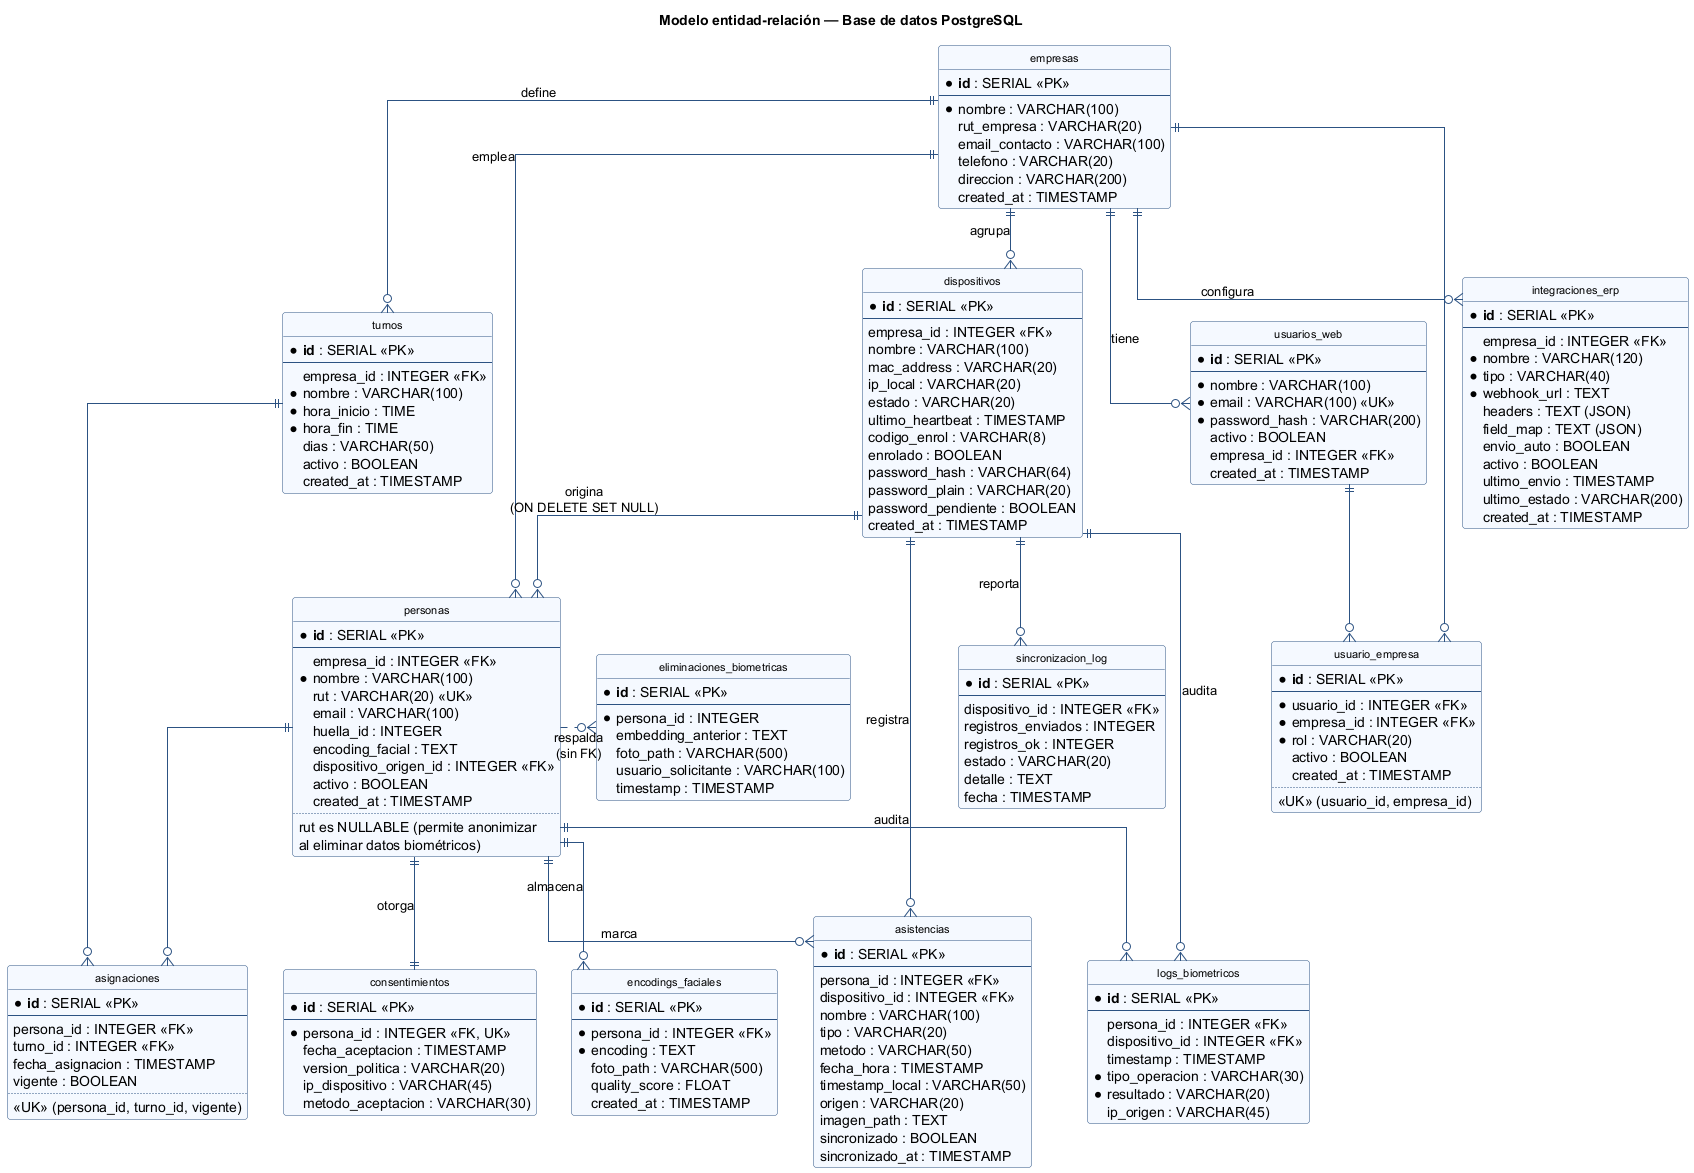
\includegraphics[width=\linewidth]{diagrams/diagrama_er_base_datos.png}
    \caption{Diagrama entidad-relación de la base de datos (14 tablas).}
    \label{fig:db-er}
\end{figure}

Las imágenes faciales, tanto las de registro como las de identificación durante la marcación, viajan del ESP32-CAM al backend por HTTP, como un JPEG crudo en formato application/octet-stream dirigido al endpoint correspondiente (POST /api/facial/registrar o POST /api/facial/identificar). El backend responde en la misma petición indicando si la foto fue aceptada, de modo que el dispositivo no necesita esperar un mensaje aparte para saber el resultado.

MQTT queda reservado para los eventos de estado del dispositivo, que son livianos y no requieren transportar una imagen. Se definen los tópicos esp32/heartbeat/<MAC> para monitorizar la actividad de los dispositivos y esp32/lwt/<MAC> para detectar desconexiones mediante el mecanismo de Last Will Testament (LWT). Para la detección activa de desconexión, se implementó el tópico esp32/ping/<MAC>: el backend publica un ping cada 30 segundos; si el ESP32-CAM no responde con un heartbeat dentro de 60 segundos, se marca como inactivo. La Figura~\ref{fig:flujo_mqtt} resume la topología de publicación y suscripción.

\begin{figure}[H]
  \centering
  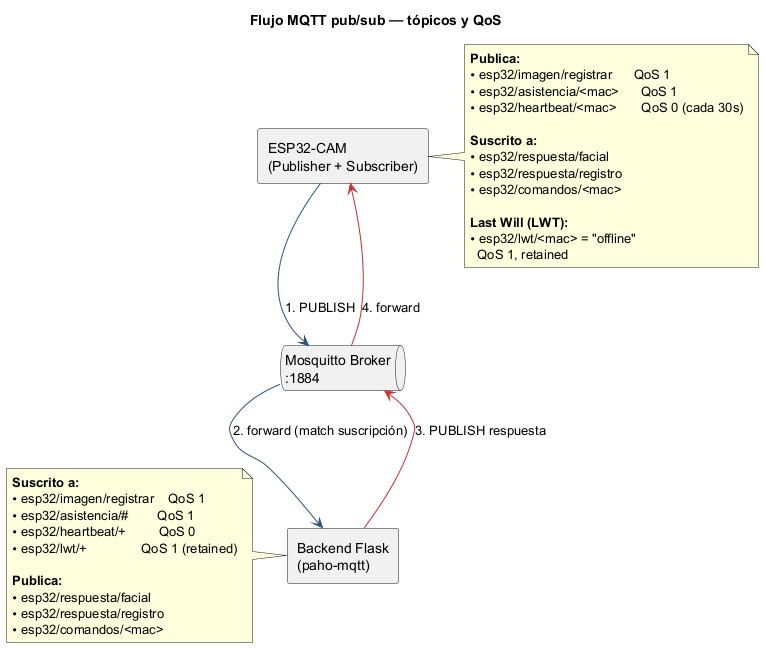
\includegraphics[width=\linewidth]{diagrams/flujo_mqtt_pub_sub.png}
  \caption{Flujo MQTT pub/sub: tópicos, direcciones y QoS entre el ESP32-CAM, el broker Mosquitto y el backend.}
  \label{fig:flujo_mqtt}
\end{figure}

\subsubsection{Implementación}

La implementación de la Iteración 3 se centró en habilitar la comunicación entre el dispositivo ESP32-CAM y el backend desarrollado en Python con Flask \cite{flask_docs}, así como en construir la base de datos PostgreSQL, accedida mediante el adaptador psycopg2 \cite{psycopg2_docs}, que soporta todo el sistema.

\paragraph{Inicialización de la base de datos}

Se implementó el módulo database.py con una función init\_db() que crea todas las tablas del sistema utilizando sentencias CREATE TABLE IF NOT EXISTS, asegurando idempotencia en los despliegues. Adicionalmente, se aplican sentencias ALTER TABLE ADD COLUMN IF NOT EXISTS para garantizar migraciones no destructivas. La función incluye la creación de índices sobre columnas frecuentemente consultadas (persona\_id, dispositivo\_id, fecha\_hora, empresa\_id) y la inserción de datos semilla (empresa por defecto, usuario administrador con contraseña hasheada).

\paragraph{Conexión Wi-Fi del ESP32-CAM y gestión de conectividad}

Para permitir la operación en red, el dispositivo implementa un mecanismo de conexión automática a Wi-Fi mediante la función tryConnectWiFi(). Esta función lee las credenciales desde wifi.json, configura el modo STA y deshabilita el ahorro de energía Wi-Fi (WIFI\_PS\_NONE) para mantener una conexión estable. La verificación continua de conectividad se realiza en verificarConexionWiFi(), que implementa un mecanismo de reintentos con backoff progresivo: tras detectar una desconexión, espera un tiempo creciente antes de reintentar (3s, 6s, 9s, 12s, 15s). Si tras 5 intentos fallidos no se logra reconectar, el dispositivo activa el Access Point como fallback.

El evento ARDUINO\_EVENT\_WIFI\_STA\_DISCONNECTED queda registrado con su código de razón y un contador de desconexiones, información expuesta a través del endpoint /wifi-diag para diagnóstico remoto.

\paragraph{Envío de imágenes faciales por HTTP: registro e identificación}

Tanto el registro como la identificación facial envían la imagen al backend de la misma manera: como JPEG crudo, sin codificarla en Base64, lo que evita el costo de procesamiento y el aumento de tamaño que implica esa codificación. Durante el registro, cuando el usuario presiona el botón de captura en la interfaz del dispositivo, el firmware toma la foto con la cámara en su calidad más alta y la sube de inmediato al backend mediante una petición POST, identificando a la persona con su RUT en una cabecera de la solicitud. El backend procesa la imagen y responde en esa misma petición si quedó aceptada o si hay que repetir la captura, lo que el dispositivo refleja en el contador de fotos de la pantalla de registro.

Durante la identificación (la consulta que ocurre al momento de marcar asistencia), el flujo es prácticamente el mismo a nivel de transporte: la imagen se captura y se envía por HTTP al endpoint de identificación, y el backend responde de forma síncrona indicando a qué persona corresponde el rostro, o un error si no encuentra coincidencia. Usar el mismo mecanismo síncrono para ambos casos simplificó el firmware, que ya no necesita dos rutas distintas para llegar al backend según el tipo de operación.

La Figura~\ref{fig:maquina_estados_esp32} ilustra la máquina de estados completa del proceso de enrolamiento biométrico en el ESP32-CAM, integrando la captura de huella digital (introducida en la Iteración 2) con el envío de la foto de referencia al backend por HTTP descrito en esta sección.

\begin{figure}[H]
  \centering
  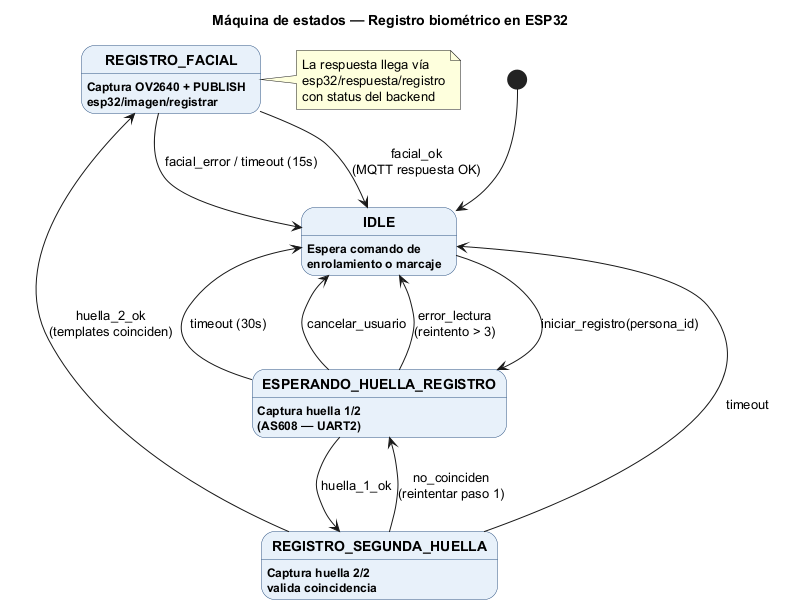
\includegraphics[width=\linewidth]{diagrams/maquina_estados_esp32.png}
  \caption{Máquina de estados del registro biométrico en el ESP32-CAM.}
  \label{fig:maquina_estados_esp32}
\end{figure}

\paragraph{Recepción de imágenes en el backend}

El backend recibe las fotos de registro e identificación a través de los endpoints REST del módulo routes/facial.py, descritos en el diseño de esta sección (ver Anexo B para el detalle completo de endpoints REST y tópicos MQTT). Al llegar una foto de registro, el backend verifica que exista consentimiento biométrico para esa persona, guarda la imagen, extrae el embedding facial y lo cifra antes de almacenarlo; si algo falla en el camino (consentimiento faltante, imagen borrosa, rostro duplicado), responde con el error correspondiente en lugar de dejar la solicitud sin respuesta.

Aparte de las imágenes, el backend mantiene un cliente MQTT para los eventos de estado del dispositivo: procesa los heartbeats, actualizando la IP y la actividad del dispositivo en la base de datos, y los mensajes de desconexión abrupta (LWT), marcándolo como inactivo. También corre en segundo plano una tarea que envía un ping cada 30 segundos a cada dispositivo enrolado, como verificación activa de que sigue en línea. Cada cambio de estado se transmite a los clientes web en tiempo real mediante streaming SSE, para que el panel se actualice sin que el administrador tenga que recargar la página.

\paragraph{Mantenimiento de la conexión MQTT en el ESP32-CAM}

El dispositivo mantiene, en paralelo a sus conexiones HTTP, un cliente MQTT que se conecta al broker si hay uno configurado y el dispositivo tiene red. Soporta URLs con esquema mqtt://, ws:// o wss:// (WebSockets seguros con TLS). Al conectarse, registra un mensaje de último aviso (LWT) para que el backend se entere si el dispositivo se cae de forma abrupta, y queda suscrito al tópico de ping para responder de inmediato cuando el backend pregunta si sigue activo. Este canal MQTT se usa únicamente para esta señalización de estado: ni el registro ni la identificación facial dependen de él.

\paragraph{Envío de datos mediante HTTP desde el ESP32-CAM}

Se implementó la capacidad del ESP32-CAM para comunicarse con la API REST del backend mediante solicitudes HTTP usando la librería HTTPClient. La función auxiliar beginHttp() configura cada petición con timeout de 10 segundos y el header X-Device-MAC para que el backend pueda identificar al dispositivo emisor. Esta función es utilizada por todos los handlers que requieren comunicación con el backend:

\begin{itemize}
    \item sincronizarPersonasDesdeBackend(): Descarga la lista completa de personas desde GET /api/personas y la persiste en personas.json.
    \item sincronizarTurnosDesdeBackend(): Descarga turnos desde GET /api/turnos.
    \item sincronizarAsignacionesDesdeBackend(): Descarga asignaciones desde GET /api/asignaciones.
    \item crearTurnoEnBackend(): Crea un turno en el backend vía POST /api/turnos.
    \item postAsistenciaEnBackend(): Envía una asistencia individual vía POST /api/asistencias.
    \item sincronizarAsistencias(): Envía un lote de asistencias pendientes vía POST /api/asistencias/sync.
\end{itemize}

\paragraph{Implementación de la API REST del backend}

El backend se implementó con Flask, organizando las rutas en blueprints independientes por dominio:
\begin{itemize}
    \item personas\_bp (routes/personas.py): CRUD de personas con validación de email, unicidad de RUT y manejo de empresa.
    \item turnos\_bp (routes/turnos.py): CRUD de turnos con filtro por empresa.
    \item asignaciones\_bp (routes/asignaciones.py): CRUD de asignaciones con verificación de pertenencia a empresa.
    \item asistencias\_bp (routes/asistencias.py): Registro de asistencias individuales y sincronización por lotes.
    \item facial\_bp (routes/facial.py): Endpoints de reconocimiento facial (registro, verificación, identificación 1:N).
    \item dispositivos\_bp (routes/dispositivos.py): Gestión y verificación de dispositivos.
    \item logs\_bp (routes/logs.py): Consulta de logs de sincronización.
    \item erp\_bp (routes/erp.py): CRUD de integraciones ERP y envío de datos.
    \item auth\_bp (routes/auth.py): Autenticación de usuarios del panel web.
\end{itemize}

Cada blueprint se registra en la aplicación Flask principal (app.py), junto con la configuración de CORS para permitir peticiones desde cualquier origen. El backend se ejecuta en el puerto 5000 con modo debug activado y recarga automática deshabilitada para evitar conflictos con el cliente MQTT.

\paragraph{Infraestructura con Docker Compose}

Para garantizar un entorno reproducible, se definió un archivo docker-compose.yml que levanta el broker Mosquitto (imagen eclipse-mosquitto:latest) con el puerto 1884 (externo, mapeado al 1883 interno) para MQTT nativo y el puerto 9001 para WebSockets expuestos, volúmenes para configuración, datos y logs persistentes, y una red bridge dedicada. El backend Flask y la base de datos PostgreSQL pueden ejecutarse en el host o en contenedores adicionales según la configuración de despliegue. La Figura~\ref{fig:docker_despliegue} presenta el diagrama de despliegue completo.

\begin{figure}[H]
  \centering
  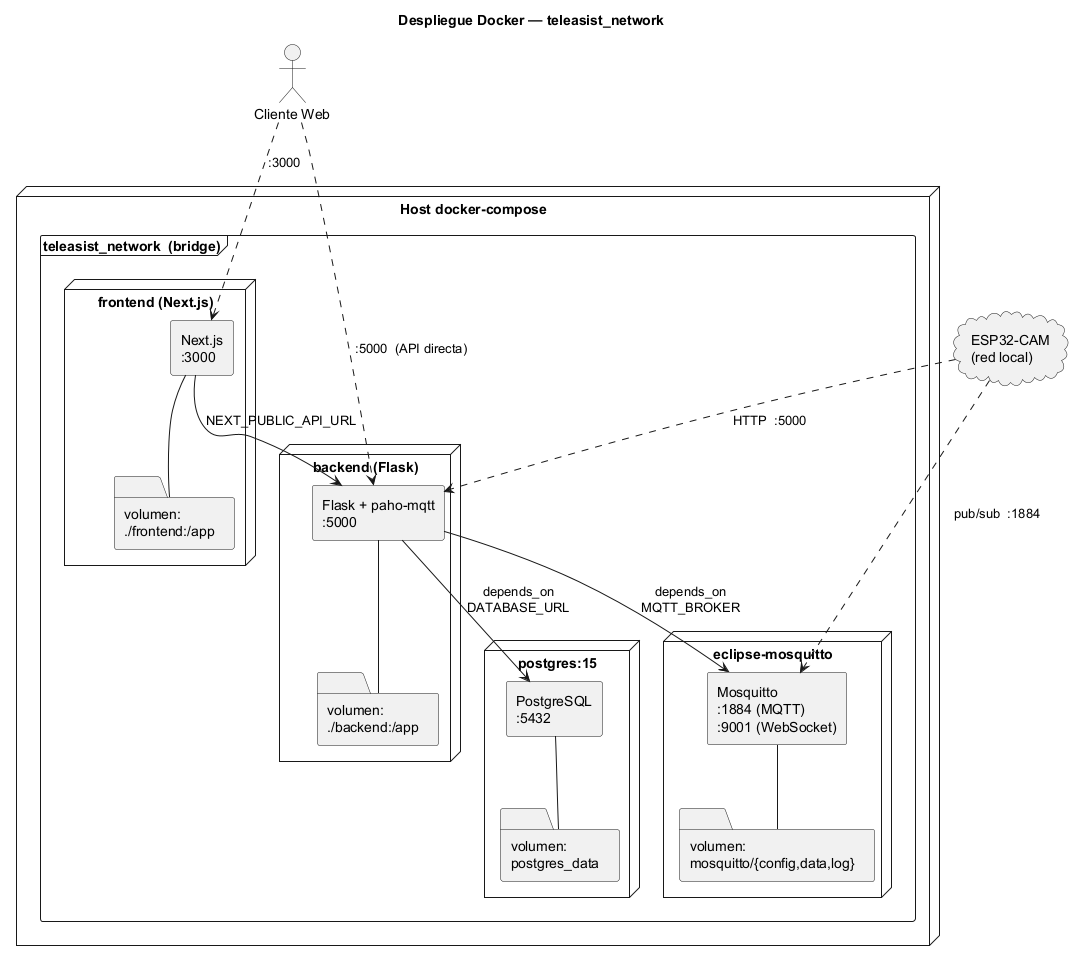
\includegraphics[width=\linewidth]{diagrams/arquitectura_despliegue_docker.png}
  \caption{Arquitectura de despliegue Docker: servicios, puertos, volúmenes y dependencias en la red.}
  \label{fig:docker_despliegue}
\end{figure}

\subsubsection{Pruebas}

Se diseñaron las siguientes pruebas para validar la comunicación y el backend:

\begin{itemize}
    \item \textbf{Prueba de conexión Wi-Fi y reconexión}: Configurar credenciales válidas en el ESP32-CAM, verificar que se conecte correctamente y obtenga una IP. Luego, apagar el router, verificar que el dispositivo detecte la desconexión mediante el evento de sistema y active el mecanismo de reintentos. Finalmente, encender el router y verificar que el dispositivo reconecte automáticamente en menos de 30 segundos.

    \item \textbf{Prueba de envío de imagen facial por HTTP}: Capturar una imagen desde el ESP32-CAM y enviarla al endpoint de registro mediante POST. Verificar que el backend reciba la imagen, la guarde en disco y responda en la misma petición indicando si la foto fue aceptada.

    \item \textbf{Prueba de heartbeat y LWT}: Verificar que, estando el ESP32-CAM conectado, el backend reciba heartbeats periódicos (cada 30 segundos) y actualice el campo ultimo\_heartbeat en la tabla dispositivos. Desconectar el dispositivo abruptamente y verificar que el mensaje LWT se publique y el backend marque el dispositivo como inactivo en menos de 10 segundos.

    \item \textbf{Prueba de ping/pong activo}: Conectar el ESP32-CAM al broker MQTT. Verificar que el backend publique esp32/ping/<MAC> periódicamente (cada 30 segundos) y que el ESP32-CAM responda con un heartbeat que contenga el campo "pong": true. Detener la conectividad del ESP32-CAM y verificar que, tras 60 segundos sin respuesta, el backend marque el dispositivo como inactivo.

    \item \textbf{Prueba de recepción de datos en backend vía HTTP}: Enviar solicitudes POST a /api/personas, /api/turnos, /api/asignaciones y /api/asistencias desde el ESP32-CAM. Verificar que cada solicitud sea procesada correctamente por el backend (código HTTP 200/201) y que los datos queden persistidos en PostgreSQL.

    \item \textbf{Prueba de sincronización por lotes}: Generar 5 marcaciones offline en el ESP32-CAM, conectar el dispositivo a la red y ejecutar la sincronización. Verificar que los 5 registros lleguen al backend vía POST /api/asistencias/sync, que se inserten correctamente y que el dispositivo marque cada registro como sincronizado = true.

    \item \textbf{Prueba de inicialización de base de datos}: Ejecutar init\_db() sobre una base de datos vacía. Verificar que se creen las 14 tablas, los índices y los datos semilla (empresa por defecto y usuario administrador) sin errores.

    \item \textbf{Prueba de latencia de transmisión}: Medir el tiempo total desde que el ESP32-CAM envía una imagen por HTTP hasta que recibe la respuesta de confirmación del backend. Se espera un tiempo menor a 5 segundos en condiciones de red local.
\end{itemize}

\paragraph{Nuevos tópicos MQTT para control y notificación}

En iteraciones posteriores se agregaron los siguientes tópicos al ecosistema MQTT:

\begin{itemize}
    \item backend/comando/<MAC>: Permite al backend enviar comandos remotos al ESP32-CAM. La función enviar\_comando\_dispositivo() en mqtt\_handler.py publica un JSON con el campo comando en este tópico.

    \item backend/notificacion/<MAC>: Utilizado por el módulo eventos\_mqtt.py para notificar a los dispositivos que deben sincronizar sus datos. Cada vez que se crea, actualiza o elimina una persona, turno o asignación, la función notificar\_sincronizacion() publica un mensaje indicando el tipo de entidad y la acción realizada.

    \item esp32/huella/resultado/<huella\_id>: Tópico en el que el ESP32-CAM publica el resultado del enrolamiento de una huella. El backend se suscribe a esp32/huella/resultado/\# y procesa la respuesta, actualizando la persona correspondiente y notificando a través de SSE.
\end{itemize}

\paragraph{Módulo eventos\_mqtt.py}

Se implementó el módulo eventos\_mqtt.py con la función notificar\_sincronizacion(empresa\_id, tipo, accion, registro\_id). Esta función consulta los dispositivos enrolados de la empresa y publica un mensaje en backend/notificacion/<MAC> por cada uno, permitiendo que los ESP32-CAM reciban notificaciones en tiempo real sobre cambios en personas, turnos y asignaciones. Es invocada desde routes/personas.py, routes/turnos.py y routes/asignaciones.py tras cada operación de creación, actualización o eliminación.

\paragraph{Streaming SSE de huellas}

Para mantener actualizados los clientes web durante el enrolamiento de huellas, se implementó el endpoint GET /sse/huellas en app.py. La función broadcast\_huella\_update() difunde los resultados del enrolamiento (recibidos por MQTT en esp32/huella/resultado/\#) a todos los clientes conectados al SSE, permitiendo que el panel web muestre en tiempo real el progreso del registro biométrico.

\subsubsection{Refinamientos posteriores}

\begin{itemize}
    \item \textbf{Decorador @requiere\_dispositivo\_enrolado}: definido en routes/auth.py, valida que el dispositivo asociado a la petición (request.dispositivo\_id) exista en la tabla dispositivos con enrolado = TRUE, devolviendo 403 en caso contrario. Se aplica sobre endpoints biométricos sensibles como /api/facial/registrar, evitando que un dispositivo no autorizado opere sobre datos biométricos.

    \item \textbf{Integridad referencial con ON DELETE SET NULL y RUT nullable}: la columna dispositivo\_origen\_id de la tabla personas (y dispositivo\_id de asistencias) se definió con REFERENCES dispositivos(id) ON DELETE SET NULL, de modo que eliminar un dispositivo no elimina en cascada las personas ni asistencias asociadas, sino que conserva el historial con la referencia en NULL. De forma análoga, la columna rut de personas se migró a nullable (ALTER TABLE personas ALTER COLUMN rut DROP NOT NULL) para permitir el borrado de datos sensibles de una persona sin perder su historial de asistencias.
\end{itemize}


%% ============================================================
%% ITERACIÓN 4: Reconocimiento facial, anti-spoofing y cifrado
%% ============================================================

\subsection{Iteración 4: Reconocimiento facial, anti-spoofing y cifrado biométrico}

Esta iteración incorpora el procesamiento biométrico en el backend: reconocimiento facial con DeepFace, validación anti-spoofing y cifrado de embeddings faciales. El sistema pasa de solo transmitir imágenes a realizar verificación e identificación biométrica.

\subsubsection{Análisis}

Para incorporar el reconocimiento facial al sistema, se evaluaron diversas librerías y modelos de deep learning. Se seleccionó DeepFace por las siguientes razones:

\begin{itemize}
    \item Soporta múltiples modelos de reconocimiento facial (Facenet, VGG-Face, ArcFace, etc.) y detectores (RetinaFace, MTCNN, OpenCV, etc.).
    \item Incluye funcionalidad de anti-spoofing integrada, capaz de distinguir entre un rostro real y una fotografía o pantalla, analizando textura, profundidad y reflectancia de la piel.
    \item Su API en Python es sencilla de integrar con Flask y compatible con las imágenes JPEG capturadas por la cámara OV2640 del ESP32-CAM.
    \item Facenet genera embeddings de 128 dimensiones, optimizando el almacenamiento y la velocidad de comparación.
\end{itemize}

Se identificaron los siguientes requisitos funcionales para esta iteración:

\begin{itemize}
    \item \textbf{Registro facial}: Recibir una imagen del ESP32-CAM, extraer el embedding facial, validar que el rostro no esté duplicado en la base de datos (detección de identidades repetidas) y almacenar el embedding cifrado.
    \item \textbf{Identificación 1:N}: Dada una imagen capturada en vivo, comparar su embedding contra todos los embeddings almacenados y retornar la identidad con mayor coincidencia, si supera el umbral de similitud.
    \item \textbf{Verificación 1:1}: Dada una imagen y un rut, verificar si la imagen corresponde a la persona declarada.
    \item \textbf{Anti-spoofing}: Detectar intentos de suplantación mediante fotografías impresas, pantallas de dispositivos o máscaras, rechazando la captura si no se detecta un rostro real.
    \item \textbf{Cifrado de embeddings}: Los vectores de características faciales (embeddings) son datos biométricos sensibles. Para protegerlos, se deben cifrar antes de persistirlos en la base de datos, utilizando una clave derivada de una variable de entorno.
    \item \textbf{Consentimiento biométrico}: Todo registro facial debe estar precedido por la aceptación explícita de una política de privacidad por parte del trabajador, en cumplimiento de la normativa de protección de datos.
\end{itemize}

\subsubsection{Diseño}

El flujo de procesamiento facial se divide en tres operaciones principales:

\begin{enumerate}
    \item \textbf{Registro} (POST /api/facial/registrar):
    \begin{itemize}
        \item Recibe la imagen como JPEG crudo (application/octet-stream) con el RUT en un header HTTP, que es como la envía el dispositivo, o como JSON con la imagen en Base64, opción que se mantiene para clientes web.
        \item Verifica que exista consentimiento biométrico en la tabla consentimientos. Si no existe, rechaza con HTTP 403.
        \item Guarda la imagen como static/previews/<id>.jpg.
        \item Aplica un \textbf{filtro de calidad de imagen} que mide la nitidez mediante la varianza del Laplaciano \cite{pech2000_laplacian}. Si la imagen es demasiado plana o borrosa (por debajo de un umbral configurable, 50 por defecto), se rechaza como posible intento de suplantación (foto de pantalla o papel) antes de llegar a DeepFace, ahorrando procesamiento innecesario del modelo.
        \item Extrae el embedding con DeepFace usando el modelo Facenet y un detector configurable mediante variable de entorno (FACIAL\_DETECTOR), utilizando MTCNN por defecto por su velocidad (tres veces más rápido que RetinaFace con precisión comparable) y sin anti-spoofing en esta etapa.
        \item Cifra el embedding con Fernet y lo almacena en la tabla encodings\_faciales, que permite acumular múltiples fotos de referencia por persona con distintos ángulos e iluminación, mejorando la precisión en subsecuentes identificaciones.
    \end{itemize}

    El flujo completo de enrolamiento biométrico, desde la creación de la persona en el panel web por parte del administrador, pasando por el registro de huella en dos pasos en el ESP32-CAM, hasta la captura facial enviada por HTTP al backend donde se extrae, cifra y almacena el embedding, se ilustra en el diagrama de secuencia de la Figura~\ref{fig:flujo_enrolamiento} del Anexo C.

    \item \textbf{Identificación 1:N} (POST /api/facial/identificar):
    \begin{itemize}
        \item Recibe la imagen como JPEG crudo (application/octet-stream) desde el ESP32-CAM, o como JSON con Base64 desde la web.
        \item Aplica el mismo filtro de calidad Laplacian como barrera anti-spoofing previa, rechazando imágenes de baja nitidez antes de invocar DeepFace.
        \item Extrae el embedding con DeepFace (anti-spoofing activado mediante anti\_spoofing=True).
        \item Consulta una caché en memoria de embeddings (con TTL configurable, 60 segundos por defecto). Si la caché expiró, recarga todos los embeddings desde la base de datos. Para cada persona, compara contra todos los embeddings almacenados en encodings\_faciales (multi-encoding) y selecciona la menor distancia. Esto mejora la precisión porque el sistema puede reconocer a un trabajador aunque la captura en vivo tenga una iluminación o ángulo diferentes a los de su foto de registro.
        \item Si la menor distancia es inferior al umbral (10.0 para Facenet), retorna el rut correspondiente. En caso contrario, retorna HTTP 404.
    \end{itemize}

    El ciclo de marcaje automático por centinela facial, en el que cada 6 segundos el ESP32-CAM evalúa el sensor PIR, captura una imagen, la envía por HTTP al endpoint de identificación, y según la respuesta del backend registra la asistencia y dispara el push asíncrono a los ERP configurados, se presenta en el diagrama de secuencia de la Figura~\ref{fig:flujo_marcaje} del Anexo C, dado su tamaño.

    \item \textbf{Verificación 1:1} (POST /api/facial/verificar):
    \begin{itemize}
        \item Recibe rut e imagen (Base64).
        \item Descifra todos los embeddings almacenados para esa persona en encodings\_faciales y extrae el embedding de la imagen capturada (con anti-spoofing activado).
        \item Calcula la distancia euclidiana contra cada embedding de referencia y selecciona la menor. Si es menor que 10.0, retorna éxito con el nivel de confianza calculado como max(0, (1 - distancia/20) * 100).
    \end{itemize}
\end{enumerate}

El modelo seleccionado es Facenet por su equilibrio entre precisión y tamaño de embedding (128 dimensiones). El detector facial es configurable mediante variable de entorno (FACIAL\_DETECTOR), utilizando MTCNN por defecto. Si bien RetinaFace ofrece mayor robustez ante variaciones extremas de pose e iluminación, MTCNN es tres veces más rápido y mantiene una precisión comparable para las condiciones típicas de una cámara de control de asistencia (rostro frontal a corta distancia), lo que lo hace más adecuado para un dispositivo embebido como el ESP32-CAM. El umbral de 10.0 para la distancia euclidiana fue elegido con base en la documentación de DeepFace y ajustes empíricos realizados durante el desarrollo.

Para el cifrado de embeddings se utiliza el algoritmo Fernet (AES-128 en modo CBC con HMAC-SHA256 para autenticación), parte de la librería cryptography de Python. La clave de cifrado se deriva aplicando SHA-256 a una variable de entorno (BIOMETRIC\_KEY), garantizando que los embeddings nunca se almacenen en texto plano en la base de datos.

\subsubsection{Implementación}

\paragraph{Procesamiento de imágenes en el backend}

El módulo routes/facial.py implementa los tres endpoints descritos en el diseño. Las funciones auxiliares incluyen:

\begin{itemize}
    \item \_validar\_calidad\_imagen(img\_path): Aplica el filtro Laplaciano (varianza del Laplaciano) sobre la imagen decodificada para medir su nitidez. Si el valor está por debajo del umbral configurable en FACIAL\_NITIDEZ\_UMBRAL (50 por defecto), la imagen se considera borrosa o plana (posible foto de pantalla o papel) y se rechaza antes de llegar a DeepFace, funcionando como una capa adicional de anti-spoofing.
    \item extraer\_embedding(img\_path, anti\_spoofing): Invoca DeepFace.represent() con el modelo Facenet pre-cargado y el detector configurable vía variable de entorno. Si anti\_spoofing=True, activa la detección de suplantación.
    \item guardar\_imagen\_de\_registro(persona\_id, imagen\_b64): Decodifica la imagen Base64, la convierte a RGB con Pillow y la guarda en static/previews/<id>.jpg.
    \item \_verificar\_consentimiento(persona\_id): Consulta la tabla consentimientos para verificar que exista un registro de aceptación.
    \item \_log\_biometrico(persona\_id, dispositivo\_id, tipo\_operacion, resultado): Inserta un registro de auditoría en logs\_biometricos.
\end{itemize}

Además, para optimizar el rendimiento, el modelo Facenet se precarga al iniciar el servidor mediante DeepFace.build\_model('Facenet', task='facial\_recognition'), eliminando la latencia de carga de pesos en la primera solicitud. Los embeddings almacenados en la base de datos se mantienen en una caché en memoria con tiempo de vida configurable (por defecto 60 segundos, mediante FACIAL\_CACHE\_TTL), evitando consultas repetitivas y descifrados a la base de datos en cada identificación. La caché se invalida automáticamente al registrar una nueva foto o al eliminar datos biométricos, garantizando consistencia.

\paragraph{Cifrado y descifrado de embeddings}

El módulo encryption.py proporciona dos funciones:

\begin{itemize}
    \item cifrar\_embedding(embedding): Serializa el embedding como JSON, lo cifra con Fernet y codifica el resultado en Base64 URL-safe.
    \item descifrar\_embedding(cifrado\_str): Decodifica el Base64, descifra con Fernet y deserializa el JSON para obtener el vector original.
\end{itemize}

\input{diagrams/08_pipeline_cifrado_biometrico.tex}

\paragraph{Actualización y eliminación de datos faciales}

Se implementó el endpoint PUT /api/facial/actualizar/<persona\_id> que permite reemplazar el embedding y la foto de una persona existente. También se implementó DELETE /api/personas/<id>/datos-biometricos que elimina el embedding facial, la huella asociada, la foto en disco y el consentimiento, pero conserva los registros de asistencia históricos. La eliminación queda registrada en la tabla eliminaciones\_biometricas para trazabilidad.

Se implementó además el endpoint POST /api/facial/agregar-foto que permite agregar fotos de referencia adicionales a una persona ya registrada, sin reemplazar las existentes. Cada nueva foto pasa por el mismo filtro de calidad Laplacian y se almacena como un nuevo registro en encodings\_faciales. Esta funcionalidad de enrolamiento progresivo permite mejorar la precisión del sistema a lo largo del tiempo: si un trabajador experimenta falsos rechazos, se le pueden agregar más fotos de referencia con distintos ángulos o condiciones de iluminación, aumentando la robustez del reconocimiento sin necesidad de rehacer el registro completo.

\subsubsection{Pruebas}

Se diseñaron las siguientes pruebas para validar el módulo de reconocimiento facial:

\begin{itemize}
    \item \textbf{Prueba de registro facial exitoso}: Enviar una imagen facial válida junto con un rut que tenga consentimiento registrado. Verificar que el backend extraiga el embedding, lo almacene cifrado y responda con HTTP 200.

    \item \textbf{Prueba de detección de duplicados}: Registrar una segunda imagen del mismo rostro para otra persona. Verificar que el backend detecte la similitud (distancia < 10.0) y rechace el registro con HTTP 409, indicando el nombre de la persona con la que coincide.

    \item \textbf{Prueba de rechazo por falta de consentimiento}: Intentar registrar un rostro para una persona sin consentimiento biométrico. Verificar que el backend rechace la operación con HTTP 403.

    \item \textbf{Prueba de identificación 1:N}: Registrar 3 personas con sus respectivas fotos. Enviar una nueva foto de una de ellas al endpoint de identificación. Verificar que el backend retorne el rut correcto.

    \item \textbf{Prueba de identificación con rostro desconocido}: Enviar una foto de una persona no registrada. Verificar que el backend retorne HTTP 404 y registre el intento fallido en logs\_biometricos.

    \item \textbf{Prueba de anti-spoofing con fotografía impresa}: Capturar una foto de un rostro registrado desde una pantalla o impresión y enviarla al endpoint de identificación. Verificar que DeepFace con anti\_spoofing=True rechace la imagen por no detectar un rostro real (excepción ValueError con mensaje ``Spoof detected'').

    \item \textbf{Prueba de resistencia a condiciones de iluminación}: Capturar imágenes del mismo rostro bajo 3 condiciones de iluminación (luz natural, luz artificial tenue, contraluz). Verificar que los 3 embeddings generados mantengan distancia euclidiana entre sí menor a 10.0 y que el sistema identifique correctamente a la persona.

    \item \textbf{Prueba de cifrado y descifrado}: Almacenar un embedding en la base de datos y verificar que el valor en la columna encoding\_facial no sea legible (no contenga los números del vector en texto plano). Luego, recuperar el registro y descifrar el embedding; verificar que el vector original se reconstruya idénticamente.

    \item \textbf{Prueba de eliminación de datos biométricos}: Ejecutar el endpoint de eliminación de datos biométricos para una persona con rostro registrado. Verificar que el embedding se elimine de la base de datos, que la foto se borre del disco, que el consentimiento se elimine, que los registros de asistencia se conserven y que quede una entrada en eliminaciones\_biometricas.

    \item \textbf{Prueba de filtro de calidad de imagen}: Enviar al endpoint de registro una imagen deliberadamente borrosa o una foto de una pantalla (baja varianza de Laplacian). Verificar que el backend rechace la imagen antes de invocar DeepFace, retornando un error de calidad insuficiente.

    \item \textbf{Prueba de múltiples fotos de referencia}: Registrar una persona con una foto frontal. Luego, agregar una segunda foto de la misma persona con distinto ángulo mediante POST /api/facial/agregar-foto. Realizar una identificación con una tercera foto y verificar que el sistema reconozca a la persona correctamente, comparando contra ambos embeddings de referencia.
    
    \item \textbf{Prueba de caché de embeddings}: Realizar una identificación exitosa y verificar los tiempos de respuesta. Realizar una segunda identificación inmediatamente después; verificar que el tiempo sea significativamente menor porque los embeddings se sirvieron desde la caché en memoria sin consultar la base de datos.
\end{itemize}

\paragraph{Endpoint identificar-o-registrar}

Se implementó el endpoint POST /api/facial/identificar-o-registrar que combina ambos flujos en una sola llamada: primero intenta identificar a la persona por su rostro; si la identificación es exitosa, retorna los datos de la persona; si falla y se proporciona un RUT con consentimiento biométrico, registra automáticamente la nueva persona con el embedding facial extraído. Este endpoint facilita el enrolamiento progresivo en el dispositivo: un trabajador puede colocarse frente al ESP32-CAM y, si ya está registrado, se marca su asistencia; si no, el sistema lo registra sobre la marcha. El endpoint incluye validación de calidad de imagen, anti-spoofing y log biométrico tanto para identificación como para registro.

\subsubsection{Refinamientos posteriores}

\begin{itemize}
    \item \textbf{Transmisión de imágenes vía octet-stream}: el envío de la imagen facial migró de un esquema basado en JSON con la foto codificada en Base64 a un envío binario directo (Content-Type: application/octet-stream) con el RUT o la MAC del dispositivo en un header HTTP (X-RUT / X-Device-MAC). El backend mantiene compatibilidad retroactiva con el formato Base64 como \textit{fallback}. El cambio elimina el overhead de codificación Base64 (aproximadamente 33\% de tamaño adicional) y simplifica el firmware, que ahora envía directamente el buffer JPEG capturado por la cámara (fb->buf, fb->len).

    \item \textbf{Captura de 3 fotos de referencia por persona}: el flujo de registro se extendió de una sola foto a tres capturas sucesivas (FOTOS\_REQUERIDAS = 3 en el firmware), idealmente frontal y de ambos perfiles, generando tres embeddings independientes almacenados en la tabla encodings\_faciales. Esto mejora la tasa de identificación ante variaciones de ángulo o iluminación, ya que la comparación 1:N evalúa contra todos los embeddings de referencia disponibles.
\end{itemize}


%% ============================================================
%% ITERACIÓN 5: Autenticación, multi-tenant y enrolamiento
%% ============================================================

\subsection{Iteración 5: Autenticación, multi-tenant y enrolamiento de dispositivos}

La quinta iteración incorpora la capa de seguridad y administración del sistema: autenticación de usuarios del panel web mediante JWT, un modelo multi-tenant que permite a múltiples empresas operar sobre la misma instancia del backend con datos aislados, y un mecanismo seguro de enrolamiento de dispositivos ESP32-CAM mediante PIN de un solo uso.

\subsubsection{Análisis}

El sistema, al estar orientado a un entorno empresarial, requiere que diferentes organizaciones puedan utilizar la misma plataforma sin que sus datos se mezclen. Asimismo, el panel web administrativo debe restringir el acceso según el rol del usuario. Finalmente, cada dispositivo ESP32-CAM debe ser vinculado de forma segura a una empresa específica, evitando que dispositivos no autorizados inyecten datos en el sistema.

Los requisitos identificados son:

\begin{itemize}
    \item \textbf{Multi-tenant}: Cada entidad (persona, turno, asignación, asistencia, dispositivo) debe pertenecer a una empresa. Las consultas deben filtrarse por empresa según el contexto del usuario autenticado. El administrador global (rol admin) tiene visibilidad sobre todas las empresas.
    \item \textbf{Autenticación JWT}: El panel web backend debe requerir autenticación para operaciones sensibles. Los tokens JWT (JSON Web Tokens), firmados con HMAC-SHA256, transportan el ID de usuario, la empresa seleccionada y su rol. Tienen expiración de 24 horas.
    \item \textbf{Roles de usuario}: Se definen tres roles jerárquicos:
    \begin{itemize}
        \item admin: Acceso total al sistema, puede crear empresas, gestionar todos los usuarios y dispositivos.
        \item empleador: Acceso limitado a los datos de su empresa; puede gestionar trabajadores, turnos y ver asistencias.
        \item trabajador: Acceso restringido a sus propios datos de asistencia.
    \end{itemize}
    \item \textbf{Enrolamiento de dispositivos}: Un administrador genera un PIN de 8 caracteres en el panel web. Ese PIN se ingresa en el ESP32-CAM (vía web embebida), que lo envía al backend junto con su MAC address. Si el PIN es válido y no ha sido usado, el dispositivo queda enrolado y asociado a la empresa correspondiente.
    \item \textbf{Auto-registro de empresas}: Se requiere un endpoint público que permita a una nueva organización registrarse de forma autónoma en el sistema, sin intervención del administrador central. La empresa proporciona sus datos (nombre, RUT, email, etc.) y los datos del usuario administrador; el sistema crea la empresa, el usuario, y la asociación entre ambos con rol admin en una sola transacción atómica, retornando un token JWT para que el nuevo administrador quede autenticado inmediatamente. Esto facilita el despliegue del sistema en nuevos clientes sin requerir configuración manual previa.
    \item \textbf{Monitorización de dispositivos}: Una vez enrolado, el ESP32-CAM envía heartbeats periódicos vía MQTT. El backend actualiza el estado del dispositivo (activo) y registra su última actividad. Un proceso watchdog marca como inactivo a los dispositivos que no han enviado heartbeat en más de 90 segundos.
\end{itemize}

\subsubsection{Diseño}

\paragraph{Modelo de datos multi-tenant}

La estrategia multi-tenant se implementa a nivel de base de datos mediante una columna empresa\_id en las tablas personas, turnos, dispositivos, integraciones\_erp y asistencias (esta última a través de la relación con personas). La tabla empresas actúa como entidad raíz del tenant. La tabla asociativa usuario\_empresa vincula usuarios con empresas y define el rol que cada usuario tiene en cada empresa, permitiendo que un mismo usuario tenga roles distintos en diferentes organizaciones.

\paragraph{Flujo de autenticación}

\begin{enumerate}
    \item El usuario envía email y contraseña al endpoint POST /api/auth/login.
    \item El backend valida las credenciales contra la tabla usuarios\_web usando bcrypt.
    \item Se consultan las empresas asociadas al usuario en usuario\_empresa.
    \item Si el usuario pertenece a una sola empresa, se selecciona automáticamente. Si pertenece a varias, se retorna la lista para que elija.
    \item Se genera un token JWT con payload: user\_id, empresa\_id, rol, persona\_id (si es trabajador) y exp (24 horas).
    \item Las peticiones subsecuentes deben incluir el header Authorization: Bearer <token>.
\end{enumerate}

Se implementan dos niveles de protección para los endpoints:
\begin{itemize}
    \item @token\_required: Exige token JWT válido.
    \item @requiere\_rol('admin', 'empleador'): Además del token, exige que el rol del usuario esté en la lista permitida.
    \item @token\_opcional: Intenta extraer el token si está presente; si no, permite el acceso sin autenticación (útil para endpoints consumidos por el ESP32-CAM, que en su lugar envían el header X-Device-MAC para identificar la empresa).
\end{itemize}

\begin{figure}[H]
  \centering
  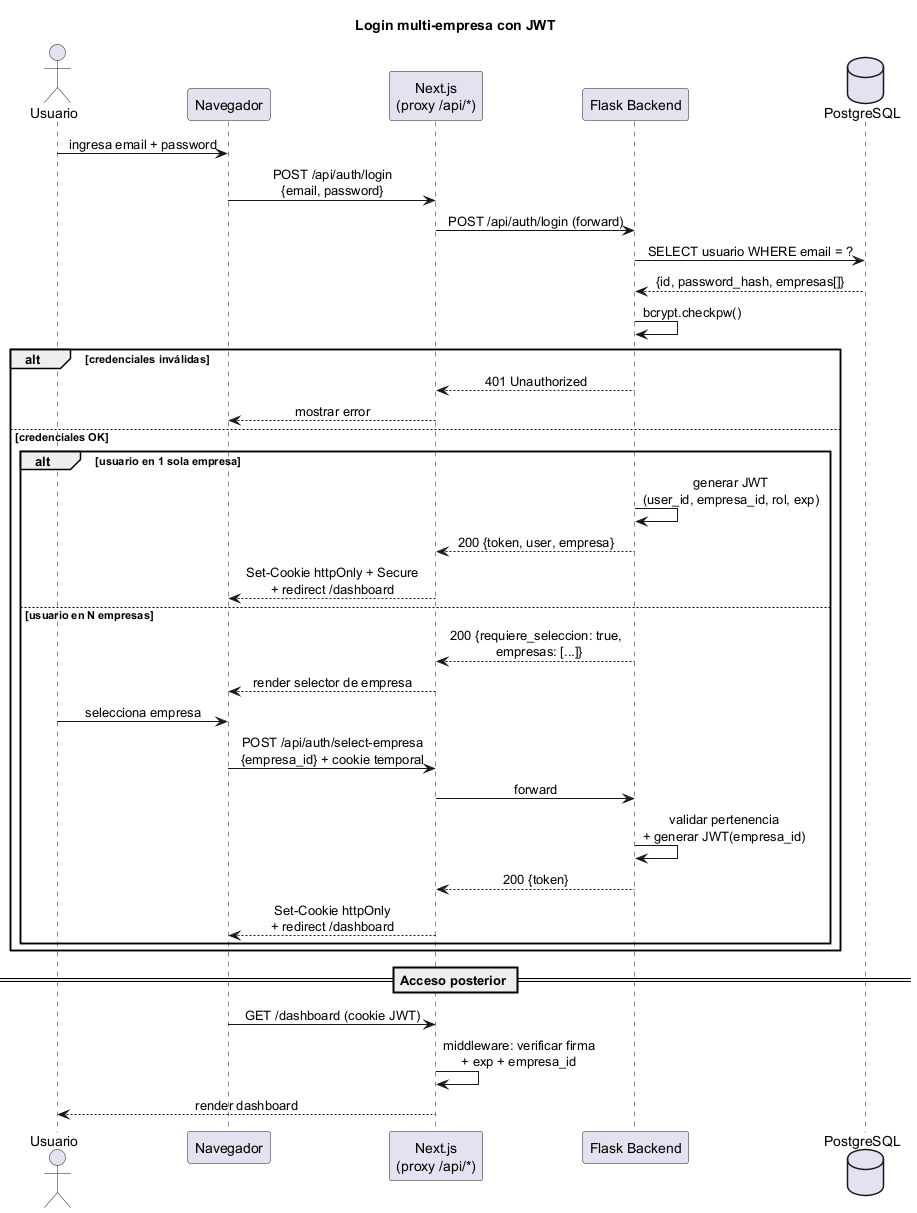
\includegraphics[width=0.95\linewidth]{diagrams/flujo_login_jwt.png}
  \caption{Diagrama de secuencia del login multi-empresa con JWT.}
  \label{fig:flujo_login_jwt}
\end{figure}

\paragraph{Flujo de enrolamiento de dispositivos}

\begin{enumerate}
    \item Un administrador o empleador accede a POST /api/dispositivos/generar-pin desde el panel web, especificando un nombre para el dispositivo. El backend genera un PIN alfanumérico de 8 caracteres (ej. A3B9XK2M) usando secrets.choice() y lo inserta en la tabla dispositivos con enrolado = FALSE.
    \item El administrador ingresa el PIN en la interfaz web del ESP32-CAM (/wifi-setup).
    \item Al guardar la configuración, el ESP32-CAM envía POST /api/dispositivos/enrolar con el PIN, su MAC address y su IP local.
    \item El backend valida el PIN, asocia la MAC y la IP al dispositivo, marca enrolado = TRUE y limpia el PIN para que no pueda ser reutilizado.
    \item A partir de este momento, el ESP32-CAM envía heartbeats periódicos y el backend lo reconoce como dispositivo autorizado de la empresa.
\end{enumerate}

\paragraph{Heartbeat y Last Will Testament (LWT)}

El ESP32-CAM publica periódicamente (cada 30 segundos) un mensaje JSON en el tópico esp32/heartbeat/<MAC> con su MAC, timestamp e IP. El backend actualiza el campo ultimo\_heartbeat y marca el estado como activo. Al conectarse al broker MQTT, el ESP32-CAM configura un mensaje LWT en el tópico esp32/lwt/<MAC> con \{"estado": "inactivo"\}. Si el dispositivo se desconecta abruptamente, el broker publica automáticamente el LWT, y el backend marca el dispositivo como inactivo.

Además del LWT y el watchdog pasivo, se implementó un ping activo como tercera capa de detección: un hilo device\_pinger() publica periódicamente (cada 30 segundos) un mensaje en el tópico esp32/ping/<MAC>. El ESP32-CAM, al recibirlo, responde inmediatamente publicando un heartbeat con el campo "pong": true. Si el backend no recibe respuesta dentro de 60 segundos, marca el dispositivo como inactivo. Este mecanismo permite detectar desconexiones incluso cuando el mensaje LWT no llega al broker (por ejemplo, por pérdida abrupta de conectividad de red). Adicionalmente, un hilo device\_watchdog ejecutado cada 60 segundos verifica qué dispositivos no han enviado heartbeat en más de 90 segundos y los marca como inactivos, constituyendo una capa de respaldo adicional.

\subsubsection{Implementación}

\paragraph{Módulo de autenticación}

El módulo routes/auth.py implementa:

\begin{itemize}
    \item login(): Valida credenciales con bcrypt, determina la empresa (con selección múltiple si aplica), vincula al trabajador con su persona\_id si el rol es trabajador, y genera el token JWT.
    \item register(): Permite a administradores y empleadores crear nuevos usuarios, asignándoles rol y empresa. Si el email ya existe, se agrega la nueva asociación usuario\_empresa en lugar de duplicar el usuario.
    \item me(): Retorna los datos del usuario autenticado, incluyendo sus empresas y rol actual.
    \item cambiar\_password(): Permite al usuario cambiar su contraseña validando la actual.
    \item generar\_pin\_enrolamiento(): Crea un PIN para enrolar un nuevo dispositivo.
    \item enrolar\_dispositivo(): Valida el PIN y completa el enrolamiento del ESP32-CAM.
    \item listar\_usuarios(), eliminar\_usuario(), listar\_empresas(), crear\_empresa(): Operaciones administrativas con control de roles.
    \item register\_company(): Endpoint público POST /api/auth/register-company que permite el auto-registro de una nueva empresa. Recibe los datos de la organización (nombre, RUT, email, teléfono, dirección) y del usuario administrador (nombre, email, contraseña). En una única transacción atómica crea la empresa, el usuario con hash bcrypt, y la asociación usuario\_empresa con rol admin. Retorna un token JWT para autenticar inmediatamente al nuevo administrador.
\end{itemize}

Los decoradores @token\_required, @token\_opcional y @requiere\_rol se definen en el mismo módulo. El decorador @token\_opcional incluye lógica para inferir la empresa a partir del header X-Device-MAC cuando no hay token JWT presente, buscando la MAC en la tabla de dispositivos. Si la MAC no existe, automáticamente crea un nuevo registro en dispositivos con estado pendiente, lo que permite que los ESP32-CAM comiencen a enviar datos incluso antes de ser formalmente enrolados.

\paragraph{Gestión de dispositivos}

El módulo routes/dispositivos.py implementa:

\begin{itemize}
    \item GET /api/dispositivos: Lista los dispositivos con su estado, MAC, IP y empresa.
    \item PUT /api/dispositivos/<id>: Actualiza el nombre del dispositivo.
    \item DELETE /api/dispositivos/<id>: Elimina un dispositivo (admin) o lo desvincula de la empresa (empleador).
    \item POST /api/dispositivos/verificar: Prueba conectividad con un dispositivo dada su IP, consultando el endpoint /estado del ESP32-CAM.
\end{itemize}

\paragraph{Monitorización vía MQTT}

En el módulo mqtt\_handler.py, la función on\_message maneja los tópicos de heartbeat y LWT:

\begin{itemize}
    \item esp32/heartbeat/<MAC>: Actualiza ultimo\_heartbeat, estado = 'activo' y opcionalmente ip\_local del dispositivo.
    \item esp32/lwt/<MAC>: Marca estado = 'inactivo' en la base de datos.
\end{itemize}

El watchdog (device\_watchdog) ejecuta un barrido inicial al arrancar (todos los dispositivos se marcan inactivos hasta que envíen su primer heartbeat) y luego verifica cada 60 segundos los heartbeats vencidos.

\subsubsection{Pruebas}

Se diseñaron las siguientes pruebas para validar la autenticación, el multi-tenant y el enrolamiento:

\begin{itemize}
    \item \textbf{Prueba de login exitoso}: Enviar credenciales válidas del administrador por defecto (admin@empresa.cl / admin123). Verificar que se reciba un token JWT, los datos del usuario y su empresa. Decodificar el token y verificar que contenga user\_id, empresa\_id y rol = admin.

    \item \textbf{Prueba de login con múltiples empresas}: Crear una segunda empresa y asignar el mismo usuario a ella con rol empleador. Iniciar sesión sin especificar empresa. Verificar que el backend retorne la lista de empresas disponibles. Luego, iniciar sesión especificando una empresa y verificar que el token refleje esa selección.

    \item \textbf{Prueba de rechazo de credenciales inválidas}: Intentar login con contraseña incorrecta. Verificar HTTP 401 y mensaje ``Credenciales inválidas''.

    \item \textbf{Prueba de acceso sin token}: Intentar acceder a GET /api/personas sin enviar header Authorization, desde un cliente sin X-Device-MAC. Verificar que el endpoint responda correctamente (acceso público o con datos limitados según el decorador).

    \item \textbf{Prueba de acceso con rol insuficiente}: Autenticarse como trabajador e intentar crear un turno (POST /api/turnos). Verificar HTTP 403 y mensaje ``Permisos insuficientes''.

    \item \textbf{Prueba de aislamiento multi-tenant}: Crear dos empresas (A y B), registrar una persona en cada una. Autenticarse como empleador de la empresa A y solicitar GET /api/personas. Verificar que solo se retornen las personas de la empresa A.

    \item \textbf{Prueba de generación de PIN}: Autenticarse como empleador y solicitar POST /api/dispositivos/generar-pin. Verificar que se reciba un PIN de 8 caracteres alfanuméricos y que en la base de datos exista un dispositivo con enrolado = FALSE.

    \item \textbf{Prueba de enrolamiento exitoso}: Con un PIN generado, enviar POST /api/dispositivos/enrolar con el PIN, una MAC y una IP. Verificar que el backend marque el dispositivo como enrolado, asocie la MAC y limpie el PIN. Verificar que el mismo PIN no pueda usarse una segunda vez (HTTP 409).

    \item \textbf{Prueba de heartbeat y estado}: Simular heartbeats desde un dispositivo enrolado. Verificar que el estado en la base de datos sea activo. Detener los heartbeats por más de 90 segundos y verificar que el watchdog marque el dispositivo como inactivo.

    \item \textbf{Prueba de LWT}: Conectar el ESP32-CAM al broker MQTT, verificar que el backend reciba el heartbeat y lo marque activo. Desconectar el dispositivo abruptamente (corte de energía). Verificar que el broker publique el LWT y el backend actualice el estado a inactivo en menos de 10 segundos.

    \item \textbf{Prueba de auto-registro de empresa}: Enviar una solicitud a POST /api/auth/register-company con los datos de una nueva empresa y su administrador. Verificar que se cree la empresa en la base de datos, que el usuario administrador se cree con contraseña encriptada (bcrypt), que exista la asociación usuario\_empresa con rol admin, y que el backend retorne un token JWT válido que permita acceder a endpoints protegidos. Verificar que un segundo intento con el mismo email de administrador retorne HTTP 409 (Conflicto).
\end{itemize}

\subsubsection{Refinamientos posteriores}

\begin{itemize}
    \item "\textbf{token\_opcional}": el decorador token\_opcional, que permite que un mismo endpoint acepte tanto usuarios web autenticados por JWT como dispositivos ESP32 identificados por el header X-Device-MAC, inicialmente creaba un registro nuevo en dispositivos si la MAC no existía en la base de datos. Este comportamiento se eliminó: ahora el decorador únicamente busca y vincula dispositivos ya existentes, dejando la creación exclusivamente al flujo explícito de enrolamiento con PIN. El cambio cierra una vía por la que un dispositivo no autorizado podía aparecer en el sistema sin pasar por el control del administrador o empleador.

    \item \textbf{PIN de enrolamiento por empresa}: la generación de PIN (POST /api/auth/dispositivos/generar-pin) quedó condicionada al rol de quien la solicita: un administrador puede generar el PIN para cualquier empresa indicada en la petición, mientras que un empleador solo puede generarlo para la empresa a la que pertenece (request.empresa\_id). El dispositivo creado queda asociado a esa empresa desde el momento de la generación del PIN, reforzando el aislamiento multi-tenant también a nivel de hardware enrolado.
\end{itemize}


%% ============================================================
%% ITERACIÓN 6: Módulo antifraude y validación previa a la captura
%% ============================================================

\subsection{Iteración 6: Módulo antifraude y validación previa a la captura}

Esta iteración implementa la prevención de suplantación de identidad en el ESP32-CAM mediante detección física de presencia, control de iluminación y procesamiento biométrico. Si bien el plan original contemplaba un sensor infrarrojo (IR) dedicado para detectar intentos de suplantación con fotografías, el enfoque implementado evolucionó hacia una solución de múltiples capas que resultó más robusta y prescindió del sensor IR adicional.

\subsubsection{Análisis}

El análisis de escenarios de suplantación identificó los siguientes vectores de ataque potenciales contra el sistema de reconocimiento facial del ESP32-CAM:

\begin{itemize}
    \item \textbf{Fotografía impresa}: Un atacante presenta una foto del rostro de un trabajador legítimo frente a la cámara.
    \item \textbf{Pantalla de dispositivo}: Un atacante muestra un video o imagen del trabajador en la pantalla de un teléfono o tablet.
    \item \textbf{Ausencia de presencia real}: La cámara captura sin que haya una persona físicamente frente al dispositivo (falsos positivos del sensor de movimiento).
\end{itemize}

Inicialmente se planificó el uso de un sensor IR dedicado que permitiera detectar la presencia de un rostro real mediante la emisión y recepción de luz infrarroja, cuya reflectancia difiere entre piel humana y superficies planas como papel o pantallas. Sin embargo, durante el desarrollo se identificaron dos factores que motivaron el cambio de estrategia:

\begin{enumerate}
    \item \textbf{Disponibilidad de GPIO}: El ESP32-CAM tiene una cantidad muy limitada de pines GPIO disponibles tras la asignación del bus paralelo de la cámara. Destinar un pin adicional al sensor IR hubiera requerido sacrificar otra funcionalidad (como el sensor PIR de presencia o el control PWM del flash).

    \item \textbf{Madurez del anti-spoofing por software}: DeepFace, la librería seleccionada para el reconocimiento facial, incorpora un detector de suplantación (\textbf{anti-spoofing}) basado en redes neuronales convolucionales que analiza micro-texturas, reflectancia de la piel y profundidad en la imagen capturada. Este detector es capaz de distinguir entre un rostro real tridimensional y una superficie plana (foto, pantalla) con una precisión comparable o superior a la de sensores IR de bajo costo como los inicialmente considerados.
\end{enumerate}

En consecuencia, se adoptó un enfoque de múltiples capas que combina:

\begin{enumerate}
    \item \textbf{Detección física de presencia (PIR)}: Un sensor infrarrojo pasivo (PIR) que detecta el calor corporal, activando el sistema de captura solo cuando hay una persona real frente al dispositivo. Esto elimina falsos positivos del software y reduce el consumo energético del sensor de huella y la cámara.
    \item \textbf{Iluminación controlada (flash PWM)}: Un destello breve y de intensidad moderada (50\% de duty cycle a 5 kHz) que ilumina el rostro durante la captura sin enceguecer a la persona. La respuesta del rostro real a esta fuente de luz puntual difiere de la de una superficie plana, aportando una capa adicional de discriminación.
    \item \textbf{Anti-spoofing por software (DeepFace)}: La capa más potente, que analiza la imagen capturada con un modelo entrenado para detectar intentos de suplantación. Las imágenes que no superan esta validación son rechazadas con una excepción ValueError que el backend traduce en un mensaje de error al ESP32-CAM.
\end{enumerate}

\subsubsection{Diseño}

\paragraph{Sensor PIR como portero del reconocimiento facial}

El lector de huellas se revisa de forma continua, sin depender del PIR: cada 500 milisegundos el sistema consulta al AS608 por si hay un dedo apoyado, de modo que una marcación por huella responda de inmediato sin esperar a que algo más la habilite. El PIR conectado al GPIO12 cumple un rol distinto, acotado al reconocimiento facial: mientras no detecta movimiento, la cámara no se usa para buscar un rostro. Al detectar movimiento (un cambio en la radiación infrarroja del entorno), el sistema enciende el flash a baja intensidad, marca que hay alguien frente al dispositivo y, si en ese momento había un bloqueo temporal del menú activo, lo anula, dando prioridad a la persona que se presentó físicamente. Tras una breve pausa de 800 milisegundos para que la lectura del sensor se estabilice, el sistema queda intentando identificar el rostro cada 6 segundos mientras dure la presencia, siempre que haya conectividad con el backend y hayan pasado al menos 8 segundos desde la última marcación. Si el PIR no vuelve a detectar movimiento durante 15 segundos, se asume que fue una falsa alarma o que la persona se retiró: se apaga el flash y el sistema vuelve a esperar sin haber intentado nada por cámara.

Esta separación evita que el reconocimiento facial, más costoso en procesamiento que la lectura de huella, se ejecute todo el tiempo sin necesidad: solo se activa cuando el PIR confirma que probablemente hay alguien frente al dispositivo.

\paragraph{Control de acceso con cooldown y bloqueo}

Para evitar marcaciones múltiples accidentales y garantizar que cada interacción sea deliberada, se implementan tres mecanismos de control:

\begin{enumerate}
    \item \textbf{Cooldown entre marcaciones} (COOLDOWN\_TIEMPO = 8000 ms): Tras una marcación exitosa, el sistema ignora nuevos intentos durante 8 segundos.
    \item \textbf{Debounce de huella} (FINGER\_DEBOUNCE = 4000 ms): Una misma huella no puede gatillar dos marcaciones en un intervalo menor a 4 segundos, evitando lecturas múltiples del mismo dedo.
    \item \textbf{Bloqueo por menú} (BLOQUEO\_MENU\_MS = 30000 ms): Cuando se utiliza la interfaz web para operaciones administrativas (registro, edición, configuración), se activa un bloqueo de 30 segundos que impide la marcación automática, evitando que la persona que está operando el menú sea registrada inadvertidamente.
\end{enumerate}

\paragraph{Firma de movimiento}

Para detectar si la escena frente a la cámara cambió entre dos capturas consecutivas (lo que indicaría una persona real moviéndose versus una foto estática), se implementa una firma de movimiento que calcula un hash reducido del buffer JPEG:

\begin{itemize}
    \item Se muestrean 128 bytes del frame capturado, distribuidos uniformemente a lo largo del buffer.
    \item Se calcula la suma acumulada de esos bytes, produciendo una firma de 32 bits.
    \item Si la diferencia entre la firma actual y la anterior supera un umbral (UMBRAL\_MOVIMIENTO = 1800), se considera que hubo movimiento real en la escena.
\end{itemize}

\subsubsection{Implementación}

\paragraph{Integración del PIR}

El sensor PIR se conecta al GPIO12 del ESP32-CAM, configurado con resistencia de pull-down interna para evitar lecturas flotantes. En el setup() se incluye una fase de calibración de 3 segundos (delay(3000)) para estabilizar el sensor antes de comenzar el bucle principal.

En el loop(), la lógica de detección sigue el siguiente flujo:

\begin{itemize}
    \item Si el PIR detecta HIGH y el flag "hayAlguienFrenteAlSensor" es falso, se activa el modo alerta y se esperan 800 ms para estabilizar la fuente de alimentación (el capacitor de 1000 $\mu$F del ESP32-CAM necesita recuperarse antes de encender la cámara).
    \item Si el PIR detecta HIGH estando ya en modo alerta, se renueva el timer de actividad.
    \item Si pasan más de 15 segundos sin detección, se desactiva el modo alerta y se retorna a reposo.
\end{itemize}

\paragraph{Flash PWM para iluminación facial}

El flash LED integrado del ESP32-CAM se controla mediante PWM en el GPIO4, configurado como salida LED PWM con frecuencia de 5 kHz y resolución de 8 bits. Durante la captura de una imagen (tanto para registro como para identificación), el flash se activa con un duty cycle del 50\% (FLASH\_PWM\_DUTY\_50 = 128) durante 150-200 milisegundos, tiempo suficiente para que el sensor OV2640 ajuste su exposición.

La secuencia de captura es la siguiente:
\begin{enumerate}
    \item Encender flash al 50\% (ledcWrite(FLASH\_PIN, 128)).
    \item Esperar 150 ms para estabilización del sensor.
    \item Capturar el frame (esp\_camera\_fb\_get()).
    \item Apagar el flash inmediatamente (ledcWrite(FLASH\_PIN, 0)).
    \item Procesar o transmitir el frame.
\end{enumerate}

Este enfoque minimiza el tiempo total de encendido del flash y, por tanto, el consumo eléctrico y la molestia para el usuario.

\paragraph{Señalización mediante el LED verde}

Además de la iluminación para captura, que usa el flash, el resultado de una operación se señaliza con el LED verde integrado en el dispositivo:

\begin{itemize}
    \item \textbf{Éxito} (flashExito()): el LED parpadea dos veces (150 ms encendido, 150 ms apagado en cada destello).
    \item \textbf{Error} (flashError()): no hay señal luminosa propia; la función queda como punto de extensión reservado en el firmware para una señal de error dedicada (por ejemplo, un patrón distinto de parpadeo o un LED rojo adicional).
\end{itemize}

El parpadeo del LED verde permite al usuario confirmar de un vistazo que su marcación se registró, sin necesidad de mirar una pantalla. La ausencia de una señal equivalente para el caso de error es una limitación reconocida del prototipo (Sección~\ref{sec:limitaciones}), ya que actualmente un error solo es visible al consultar la vista web del dispositivo.

\paragraph{Validación anti-spoofing en el backend}

La validación anti-spoofing se ejecuta en el backend, no en el ESP32-CAM, debido a las limitaciones de procesamiento del microcontrolador. La función extraer\_embedding() en routes/facial.py recibe el parámetro anti\_spoofing=True para los endpoints de identificación y verificación, lo que activa el detector de suplantación de DeepFace. Si la imagen no supera la validación (por ser una foto, pantalla o carecer de características faciales reales), DeepFace lanza una excepción ValueError que el backend captura y traduce en una respuesta HTTP 400 con el mensaje ``Spoof detected''.

\subsubsection{Pruebas}

Se diseñaron las siguientes pruebas para validar el módulo antifraude:

\begin{itemize}
    \item \textbf{Prueba de detección PIR}: Situar a una persona a 50 cm del dispositivo. Verificar que el PIR detecte el movimiento en menos de 1 segundo y que el sistema transicione a modo activo. Retirar a la persona y verificar que tras 15 segundos sin detección, el sistema retorne a reposo.

    \item \textbf{Prueba de falsos positivos del PIR}: Dejar el dispositivo en una habitación vacía durante 10 minutos y monitorear los logs. Verificar que no se active el modo de captura sin presencia humana real (tolerancia máxima: 1 falso positivo por hora).

    \item \textbf{Prueba de cooldown}: Realizar una marcación exitosa por huella. Intentar inmediatamente una segunda marcación. Verificar que el sistema rechace el intento por estar en período de cooldown (8 segundos).

    \item \textbf{Prueba de debounce de huella}: Mantener el dedo presionado sobre el sensor AS608 durante 5 segundos. Verificar que solo se registre una marcación, no múltiples.

    \item \textbf{Prueba de bloqueo por menú}: Acceder a la vista /register desde el navegador. Mientras la página está abierta, intentar provocar una marcación automática con huella. Verificar que el sistema esté bloqueado durante 30 segundos.

    \item \textbf{Prueba de anti-spoofing con fotografía}: Imprimir una foto de un rostro registrado y presentarla frente al ESP32-CAM con el PIR activado (para ello, mover la foto simulando una persona). Verificar que DeepFace rechace la imagen con anti\_spoofing=True y que el backend retorne HTTP 400.

    \item \textbf{Prueba de anti-spoofing con pantalla}: Reproducir un video del rostro de una persona registrada en un teléfono móvil y presentarlo frente al ESP32-CAM. Verificar que el sistema rechace la identificación.

    \item \textbf{Prueba de flash PWM}: Durante una captura, medir con un osciloscopio o cámara de alta velocidad que el flash se encienda al 50\% de duty cycle durante no más de 200 ms. Verificar que la iluminación sea suficiente para obtener una imagen nítida del rostro.

    \item \textbf{Prueba de señalización}: Provocar una marcación exitosa y verificar que el LED verde parpadee dos veces. Provocar un error (huella no reconocida) y verificar que no se emita ninguna señal luminosa.
\end{itemize}


%% ============================================================
%% ITERACIÓN 7: Panel web backend e integración con ERP
%% ============================================================

\subsection{Iteración 7: Panel web backend e integración con ERP}

La séptima iteración incorpora el panel de administración web del backend y el módulo de integración con sistemas ERP externos, permitiendo que los datos de asistencia capturados por el dispositivo IoT sean automáticamente transmitidos a plataformas empresariales de recursos humanos o nómina.

\subsubsection{Análisis}

El sistema, hasta esta iteración, permite registrar asistencias y almacenarlas en la base de datos, pero carece de una interfaz administrativa centralizada y de un mecanismo para integrar los datos con sistemas ERP existentes. Se identificaron los siguientes requisitos:

\begin{itemize}
    \item \textbf{Panel web administrativo}: Una interfaz web que permita a administradores y empleadores gestionar personas, turnos, asignaciones, visualizar asistencias, administrar dispositivos enrolados y configurar integraciones ERP. Debe ser accesible vía navegador sin dependencia del ESP32-CAM.
    \item \textbf{API REST completa y documentada}: Todos los blueprints implementados en iteraciones anteriores deben consolidarse como una API REST coherente, con métodos HTTP estándar, respuestas JSON estructuradas y manejo de autenticación por JWT.
    \item \textbf{Integración con ERP vía webhooks}: Permitir configurar múltiples destinos ERP, cada uno con su propia URL de webhook, headers personalizados (ej. tokens de autenticación) y mapeo de campos (field mapping) para adaptar el formato de los datos de asistencia al esquema esperado por cada ERP.
    \item \textbf{Envío automático}: Las asistencias registradas deben enviarse automáticamente a los ERP configurados, en un hilo separado para no bloquear la respuesta HTTP al dispositivo.
    \item \textbf{Test de conectividad}: Cada integración ERP debe poder probarse manualmente desde el panel web antes de activar el envío automático.
\end{itemize}

\subsubsection{Diseño}

\paragraph{Arquitectura del backend}

El backend se organiza en 9 blueprints de Flask, cada uno con responsabilidades bien definidas:

\begin{enumerate}
    \item auth\_bp: Autenticación JWT, registro de usuarios, gestión de empresas, enrolamiento de dispositivos.
    \item personas\_bp: CRUD de personas con consentimiento biométrico y eliminación de datos sensibles.
    \item turnos\_bp: CRUD de turnos con filtro por empresa.
    \item asignaciones\_bp: CRUD de asignaciones persona-turno.
    \item asistencias\_bp: Registro de asistencias individuales y sincronización por lotes.
    \item facial\_bp: Registro, verificación e identificación facial con anti-spoofing y cifrado.
    \item dispositivos\_bp: Gestión de dispositivos enrolados y verificación de conectividad.
    \item logs\_bp: Consulta de logs de sincronización y logs biométricos.
    \item erp\_bp: CRUD de integraciones ERP, envío de datos y test de conectividad.
\end{enumerate}

\paragraph{Diseño del módulo ERP}

La integración con ERP se basa en el patrón webhook saliente: cuando se registra una asistencia, el backend notifica a cada ERP configurado mediante una solicitud HTTP POST al webhook correspondiente, con los datos de la marcación en el cuerpo JSON.

Cada integración ERP se configura con los siguientes parámetros:

\begin{itemize}
    \item nombre: Identificador descriptivo (ej. ``Softland RRHH'').
    \item tipo: Clasificación del ERP (generic, softland, defontana, sap).
    \item webhook\_url: Endpoint HTTP donde el ERP espera recibir los datos.
    \item headers: Objeto JSON con headers HTTP personalizados (ej. \{"Authorization": "Bearer <token>"\}).
    \item field\_map: Objeto JSON que mapea los campos estándar del sistema (rut, nombre, tipo, metodo, fecha\_hora) a los nombres de campo esperados por el ERP.
    \item envio\_auto: Booleano que indica si el envío se realiza automáticamente al registrar cada asistencia, o solo manualmente.
    \item activo: Booleano para habilitar o deshabilitar temporalmente la integración sin eliminarla.
\end{itemize}

El field mapping permite adaptar el formato de salida sin modificar el código del backend. Por ejemplo, un ERP que espera los campos employee\_id, timestamp y event\_type puede configurarse con:
\begin{verbatim}
{"rut": "employee_id", "fecha_hora": "timestamp", "tipo": "event_type"}
\end{verbatim}

\begin{figure}[H]
  \centering
  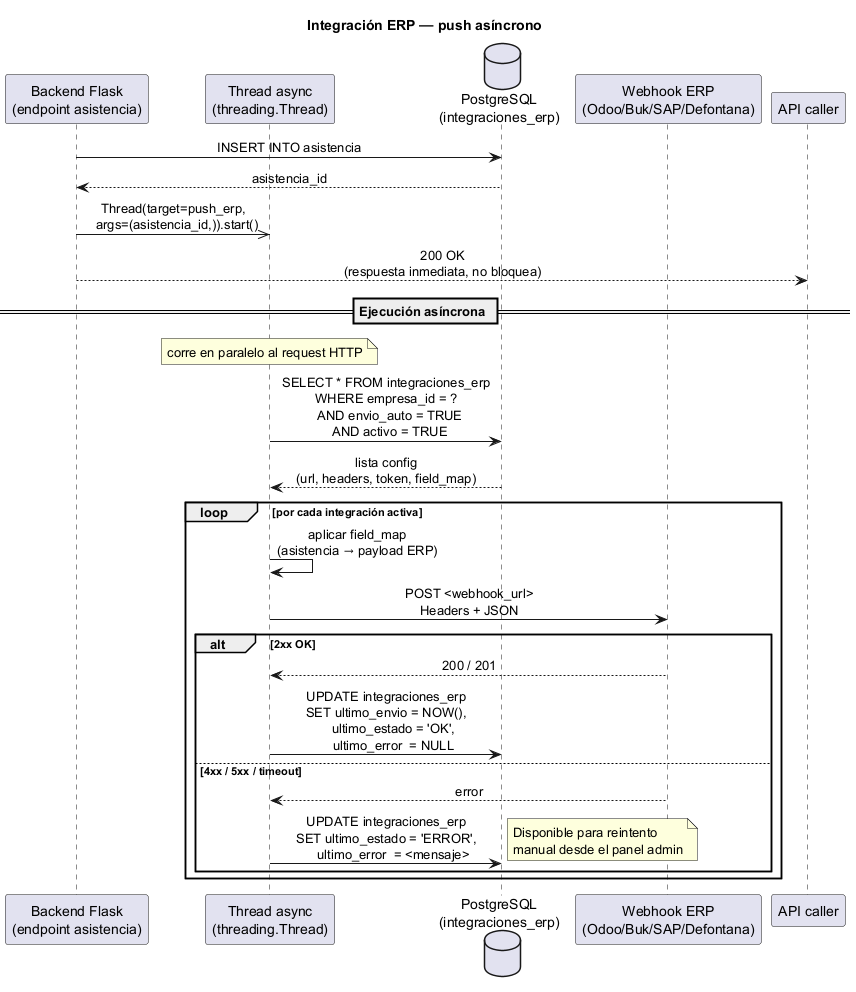
\includegraphics[width=0.95\linewidth]{diagrams/flujo_integracion_erp.png}
  \caption{Diagrama de secuencia de la integración ERP: push asíncrono con field mapping.}
  \label{fig:flujo_erp}
\end{figure}

\subsubsection{Implementación}

\paragraph{Panel web del backend}

Para complementar el backend, se desarrolló un panel web independiente (Next.js 16 \cite{nextjs_docs} con React 19 y TypeScript) cuyo módulo principal es la gestión del dispositivo IoT. Este panel, accesible desde cualquier navegador moderno, permite al administrador:

\begin{itemize}
    \item Visualizar el estado online/offline de cada dispositivo enrolado en tiempo real mediante tarjetas con código de colores, indicador animado (live-dot) y la IP como enlace clickable con la leyenda ``Misma red requerida''.
    \item Generar el PIN de 8 caracteres necesario para enrolar un nuevo ESP32-CAM.
    \item Probar la conectividad activa con un dispositivo específico consultando su endpoint /estado (variable NEXT\_PUBLIC\_DEVICE\_BASE\_URL, por defecto http://192.168.4.1).
    \item Renombrar y eliminar dispositivos registrados.
    \item Acceder a los logs de sincronización generados por el dispositivo.
    \item Acceder a las funcionalidades complementarias de gestión: personas, turnos, asignaciones, asistencias, integración ERP, usuarios y empresas.
\end{itemize}

El estado en tiempo real se obtiene mediante dos mecanismos complementarios. El principal es un hook useDeviceWebSocket que utiliza EventSource para conectarse directamente al endpoint SSE del backend (http://localhost:5000/sse/devices), recibiendo eventos con el id, nombre, IP, estado y timestamp del último heartbeat de cada dispositivo. Como respaldo, un temporizador ejecuta una consulta REST cada 15 segundos (GET /api/dispositivos) para actualizar el estado si la conexión SSE se interrumpe. El estado online se calcula verificando que el campo estado sea 'activo' y que el ultimo\_heartbeat esté dentro de los últimos 5 minutos; si alguna condición falla, el dispositivo se considera offline.

El panel web se comunica con el backend Flask mediante un proxy interno (app/api/\_proxy.ts) que reenvía las peticiones REST a la API, evitando problemas de CORS. La conexión SSE, por su parte, se realiza directamente al backend en el puerto 5000 sin pasar por el proxy, ya que requiere una conexión persistente text/event-stream. La aplicación está protegida por un middleware de autenticación que valida el token JWT y restringe el acceso según el rol del usuario (admin, empleador, trabajador). El frontend se compila con Docker en un build multi-etapa usando output: 'standalone' para producir una imagen optimizada lista para producción.

Para mantener la consistencia visual entre el panel web y la interfaz embebida del ESP32-CAM, las 9 vistas HTML del dispositivo (index.html, register.html, gestion.html, personas.html, turnos.html, asignaciones.html, asistencias.html, logs.html y wifi-setup.html) fueron actualizadas para adoptar la misma paleta oscura, tipografía y sistema de componentes del panel SAS. Se utilizaron variables CSS para la paleta cromática, diseño basado en tarjetas (cards) para la disposición del contenido, y componentes reutilizables para botones, tablas y formularios, logrando que ambas interfaces presenten una experiencia de usuario unificada.

Adicionalmente, el panel web incorpora las siguientes funcionalidades complementarias:

\begin{itemize}
    \item \textbf{Auto-registro de empresas}: La pantalla de inicio de sesión incluye un modo de registro que permite a nuevas empresas crear su cuenta directamente, invocando al endpoint público POST /api/auth/register-company. El formulario solicita nombre de la empresa y datos del administrador de la empresa (nombre, email, contraseña), y al enviarlo crea la organización, el usuario administrador y retorna un token JWT para acceso inmediato.
    \item \textbf{Captura facial por webcam}: El formulario de registro facial en el panel web utiliza la API navigator.mediaDevices.getUserMedia() para capturar fotografías directamente desde la cámara del navegador, eliminando la necesidad de subir archivos desde el sistema de archivos local. La interfaz permite visualizar la vista previa en vivo, capturar, previsualizar y confirmar o repetir la toma, con liberación adecuada del stream al cancelar.
    \item \textbf{Edición de usuarios del sistema}: Los administradores y empleadores pueden editar los datos de los usuarios del sistema (nombre, email, rol, contraseña, estado activo/inactivo) mediante un formulario modal que reutiliza la interfaz de registro en modo edición. Las actualizaciones son parciales: solo se envían los campos modificados.
\end{itemize}

\paragraph{Endpoint de configuración ERP para el ESP32-CAM}

Para que el ESP32-CAM pueda notificar asistencias directamente a los ERP configurados (incluso si el backend central no está disponible), se implementó el endpoint GET /api/dispositivos/erp-config, que retorna la lista de integraciones ERP activas con envío automático habilitado. El ESP32-CAM consulta este endpoint cada hora y almacena la configuración en /erp-config.json, permitiéndole enviar marcaciones a los ERP incluso durante desconexiones parciales.

\paragraph{Contraseñas para autenticación de dispositivos}

Para reforzar la seguridad en la comunicación entre el backend y los ESP32-CAM enrolados, se implementó un sistema de contraseñas de dispositivo que permite al administrador generar, gestionar y verificar credenciales específicas para cada terminal IoT. El flujo contempla cuatro operaciones:

\begin{itemize}
    \item \textbf{Generar contraseña} (POST /api/dispositivos/<id>/generar-password): El administrador solicita una nueva contraseña de 12 caracteres alfanuméricos, generada mediante secrets.choice(). El backend almacena el hash SHA256 de la contraseña, la versión en texto plano (temporal) y marca la contraseña como pendiente (password\_pendiente = TRUE). La respuesta incluye la contraseña en texto plano para que el administrador la proporcione al dispositivo.
    \item \textbf{Verificar contraseña pendiente} (GET /api/dispositivos/check-password): El ESP32-CAM, al iniciar, consulta este endpoint enviando su MAC address como header X-Device-MAC. Si hay una contraseña pendiente, el backend la retorna en texto plano para que el dispositivo la aplique localmente.
    \item \textbf{Confirmar contraseña} (POST /api/dispositivos/confirmar-password): Una vez que el dispositivo ha aplicado la contraseña localmente, confirma al backend, que limpia el texto plano (password\_plain = NULL) y desmarca el estado pendiente. A partir de este momento, solo el hash SHA256 permanece almacenado.
    \item \textbf{Eliminar contraseña} (DELETE /api/dispositivos/<id>/password): El administrador puede eliminar la contraseña de un dispositivo, limpiando el hash y el texto plano.
\end{itemize}

En el panel web, la sección de gestión de dispositivos incorpora botones para generar, regenerar y eliminar contraseñas, así como indicadores visuales del estado de la contraseña (tiene o no tiene, pendiente o confirmada).

\paragraph{Módulo de integración ERP}

El módulo routes/erp.py implementa:

\begin{itemize}
    \item \textbf{enviar\_asistencia\_a\_erps()}: Función central que itera sobre las integraciones ERP activas de una empresa, transforma los datos de la asistencia según el field mapping configurado, y envía una solicitud POST al webhook con los headers personalizados. Registra el resultado (ok o error) en la tabla integraciones\_erp (columnas ultimo\_envio y ultimo\_estado).

    \item \textbf{\_disparar\_erp\_push()}: Wrapper que ejecuta enviar\_asistencia\_a\_erps() en un hilo daemon separado, evitando que la latencia de los ERP externos afecte el tiempo de respuesta al ESP32-CAM. Esta función se invoca automáticamente desde create\_asistencia() y sync\_asistencias() cada vez que se registra una asistencia.

    \item \textbf{CRUD de integraciones}: Endpoints REST para crear, listar y eliminar configuraciones ERP.

    \item \textbf{Test de conectividad} (POST /api/erp/<id>/test): Envía un payload de prueba con datos ficticios al webhook configurado y retorna el código de respuesta y el cuerpo recibido.

    \item \textbf{Envío manual} (POST /api/erp/<id>/enviar): Envía las últimas 200 asistencias de la empresa al ERP seleccionado, útil para cargas históricas o reprocesamiento.

    \item \textbf{Estado de integración} (GET /api/erp/<id>/estado): Retorna el último envío y su estado.
\end{itemize}

\paragraph{Control remoto de dispositivos ESP32}

Se implementaron tres endpoints en routes/dispositivos.py que permiten controlar remotamente los ESP32-CAM enrolados mediante comandos MQTT:

\begin{itemize}
    \item \textbf{Registrar huella} (POST /api/dispositivos/<id>/registrar-huella): Recibe un persona\_id y envía al dispositivo el comando para iniciar el enrolamiento de una huella digital. Verifica que el dispositivo exista, que pertenezca a la empresa del usuario autenticado, y que la persona exista en la misma empresa. Utiliza enviar\_comando\_dispositivo(mac, 'registrar\_huella') para publicar el comando en backend/comando/<MAC>/registrar\_huella. El resultado del enrolamiento se recibe luego por el tópico esp32/huella/resultado/\#.

    \item \textbf{Reiniciar dispositivo} (POST /api/dispositivos/<id>/reiniciar): Envía el comando reiniciar al ESP32-CAM, provocando un reinicio remoto del dispositivo. Útil para recuperar un dispositivo que presenta fallos de conectividad o para aplicar cambios de configuración. Si el cliente MQTT no está disponible, retorna HTTP 503.

    \item \textbf{Reconectar Wi-Fi} (POST /api/dispositivos/<id>/wifi-reconnect): Envía el comando wifi-reconnect para que el dispositivo reinicie su conexión Wi-Fi. Permite recuperar un dispositivo que ha perdido la conectividad sin necesidad de intervención física.
\end{itemize}

Los tres endpoints están protegidos con \textbf{"@requiere\_rol('admin', 'empleador')"} y verifican que el dispositivo pertenezca a la empresa del usuario autenticado. Los comandos se publican en el tópico backend/comando/<MAC>/<comando> mediante la función enviar\_comando\_dispositivo() del módulo mqtt\_handler.py.

\subsubsection{Pruebas}

Se diseñaron las siguientes pruebas para validar el panel web para la gestión del dispositivo y la integración ERP:

\begin{itemize}
    \item \textbf{Prueba de streaming SSE}: Conectar el navegador a http://localhost:5000/sse/devices y verificar que se reciban eventos text/event-stream con datos JSON de los dispositivos. Simular un heartbeat desde un ESP32-CAM y verificar que el evento SSE refleje el cambio a estado activo. Desconectar el dispositivo y verificar que el evento SSE refleje el estado inactivo.

    \item \textbf{Prueba de fallback polling}: Interrumpir la conexión SSE (deteniendo el servidor backend momentáneamente). Verificar que el panel web continúe mostrando el estado de los dispositivos mediante las consultas REST periódicas (cada 15 segundos) y que al restaurar la conexión SSE se retome el streaming.

    \item \textbf{Prueba de indicador visual de dispositivo}: Verificar que cada tarjeta de dispositivo en el panel web muestre: la dirección IP como enlace clickable que abre http://<ip>/ en una nueva pestaña, un indicador animado verde/rojo (live-dot) que refleje el estado online/offline, y la leyenda ``Misma red requerida'' como sugerencia contextual.

    \item \textbf{Prueba de navegación en panel web}: Acceder a las rutas principales del backend (/health, /api/personas, /api/asistencias) sin autenticación y verificar que respondan correctamente (HTTP 200 con acceso público o HTTP 401 cuando se requiera token).

    \item \textbf{Prueba de creación de integración ERP}: Autenticarse como empleador y enviar POST /api/erp con nombre, tipo, webhook URL (usando un servidor de prueba como https://webhook.site) y field mapping. Verificar que la integración se cree con activo = TRUE y envio\_auto = TRUE.

    \item \textbf{Prueba de test de webhook}: Ejecutar POST /api/erp/<id>/test para la integración creada. Verificar que el webhook de prueba reciba un payload JSON con datos ficticios (rut = '11.111.111-1', nombre = "Test Usuario", tipo = "entrada"). Verificar que el estado se actualice en la base de datos.

    \item \textbf{Prueba de envío automático}: Registrar una asistencia real (POST a /api/asistencias) para una persona de la empresa configurada. Verificar que el servidor de prueba del webhook reciba automáticamente el payload con los datos de la asistencia.

    \item \textbf{Prueba de field mapping}: Configurar un ERP con field mapping \{"rut": "employee\_id", "tipo": "event"\}. Registrar una asistencia y verificar que el webhook reciba el payload con los campos renombrados (employee\_id en lugar de rut, event en lugar de tipo).

    \item \textbf{Prueba de envío asíncrono}: Medir el tiempo de respuesta del endpoint POST /api/asistencias cuando hay un ERP configurado cuyo webhook tarda 5 segundos en responder. Verificar que la respuesta al cliente sea inmediata (menor a 200 ms) y que el envío al ERP ocurra en segundo plano.

    \item \textbf{Prueba de tolerancia a fallos ERP}: Configurar un webhook que retorne HTTP 500. Registrar una asistencia y verificar que el sistema no falle; el error debe quedar registrado en ultimo\_estado de la integración y la asistencia debe persistirse correctamente en la base de datos.

    \item \textbf{Prueba de sincronización de configuración ERP al ESP32-CAM}: Simular la consulta GET /api/dispositivos/erp-config desde el ESP32-CAM (con header X-Device-MAC). Verificar que retorne solo las integraciones activas con envío automático de la empresa correspondiente.

    \item \textbf{Prueba de envío manual por lote}: Ejecutar POST /api/erp/<id>/enviar y verificar que se envíen correctamente los registros de asistencia recientes al webhook del ERP.
\end{itemize}

\subsubsection{Refinamientos posteriores}

\begin{itemize}
    \item \textbf{Reasignación de dispositivos entre empresas}: se agregó el endpoint PUT /api/dispositivos/<id>/reasignar, restringido al rol admin, que permite mover un dispositivo ya enrolado de una empresa a otra actualizando su columna empresa\_id. Esto resuelve el caso de dispositivos físicos que cambian de destino (por ejemplo, al reasignar hardware entre sucursales o clientes) sin requerir un nuevo proceso de enrolamiento con PIN.

    \item \textbf{Zona horaria de Chile en la integración ERP}: los timestamps enviados a los webhooks ERP se normalizan a America/Santiago mediante el módulo estándar zoneinfo, con conversión explícita antes de formatear cada fecha\_hora y timestamp del payload. Esto evita ambigüedades cuando el servidor del backend opera en UTC y el sistema ERP de destino espera horarios locales.

    \item \textbf{Soporte de múltiples fotos en el panel web}: el panel de administración construido con Next.js incorpora en la vista de cada persona la visualización de las fotos de referencia asociadas a sus distintos encodings\_faciales, reflejando en la interfaz la capacidad de multi-encoding ya descrita en la Sección 2.3.10. Asimismo, en los despliegues multi-empresa la interfaz incorpora una indicación visual de la empresa a la que pertenece cada registro, relevante para el rol admin, que puede ver datos de más de una organización.
\end{itemize}


%% ============================================================
%% ITERACIÓN 8: Sincronización diferida, logs y cierre del proyecto
%% ============================================================

\subsection{Iteración 8: Sincronización diferida, logs y cierre del proyecto}

Esta iteración integra la sincronización diferida entre el ESP32-CAM y el backend, la capa de auditoría y logs del sistema, y las herramientas de diagnóstico.

\subsubsection{Análisis}

Para que el prototipo sea viable en entornos reales, debe garantizar que ningún dato se pierda durante períodos de desconexión y que todas las operaciones críticas queden registradas para auditoría. Los requisitos identificados son:

\begin{itemize}
    \item \textbf{Sincronización diferida de asistencias}: Los registros de asistencia generados offline (marcados con sincronizado = false) deben enviarse automáticamente al backend cuando se restablezca la conectividad. El proceso debe ser idempotente: si un registro ya existe en el backend, no debe duplicarse.
    \item \textbf{Sincronización diferida de entidades}: Las personas, turnos y asignaciones creados localmente durante el modo offline deben sincronizarse con el backend, resolviendo conflictos de identificadores (IDs locales con prefijo local- versus IDs del backend).
    \item \textbf{Sincronización de configuración ERP}: La configuración de integraciones ERP debe poder descargarse desde el backend para que el ESP32-CAM pueda enviar datos de asistencia directamente a los ERP configurados.
    \item \textbf{Logs de sincronización}: Cada operación de sincronización debe registrarse en la base de datos con el conteo de registros enviados y procesados correctamente, permitiendo auditoría posterior.
    \item \textbf{Logs biométricos}: Todas las operaciones de registro, verificación e identificación facial deben quedar registradas con timestamp, resultado e IP de origen, para cumplimiento normativo.
    \item \textbf{Watchdog de dispositivos}: El backend debe monitorear continuamente el estado de los dispositivos enrolados, detectando aquellos que han dejado de comunicarse y marcándolos como inactivos.
    \item \textbf{Herramientas de diagnóstico}: Se requiere un script de prueba que permita simular asistencias faciales usando fotos almacenadas, facilitando las pruebas del sistema sin necesidad del hardware.
\end{itemize}

\subsubsection{Diseño}

\paragraph{Proceso de sincronización diferida}

El ESP32-CAM ejecuta la sincronización en dos momentos:
\begin{enumerate}
    \item \textbf{Al iniciar}: Si hay conectividad, llama a sincronizarPendientes() que ejecuta en secuencia:
    \begin{itemize}
        \item sincronizarTurnosPendientes(): Envía los turnos con sincronizado = false al backend vía POST, y actualiza sus backend\_id.
        \item sincronizarAsignacionesPendientes(): Similar para asignaciones, dependiendo de que los turnos referenciados ya tengan backend\_id.
        \item sincronizarAsistencias(): Envía un lote de asistencias con sincronizado = false vía POST /api/asistencias/sync.
    \end{itemize}
    \item \textbf{Periódicamente}: Cada 5 minutos (300,000 ms), se ejecuta sincronizarPendientes() en el bucle principal.
\end{enumerate}

Además, el ESP32-CAM consulta GET /api/dispositivos/erp-config cada hora (360,000 ms) para mantener actualizada su configuración local de webhooks ERP.

\begin{figure}[H]
  \centering
  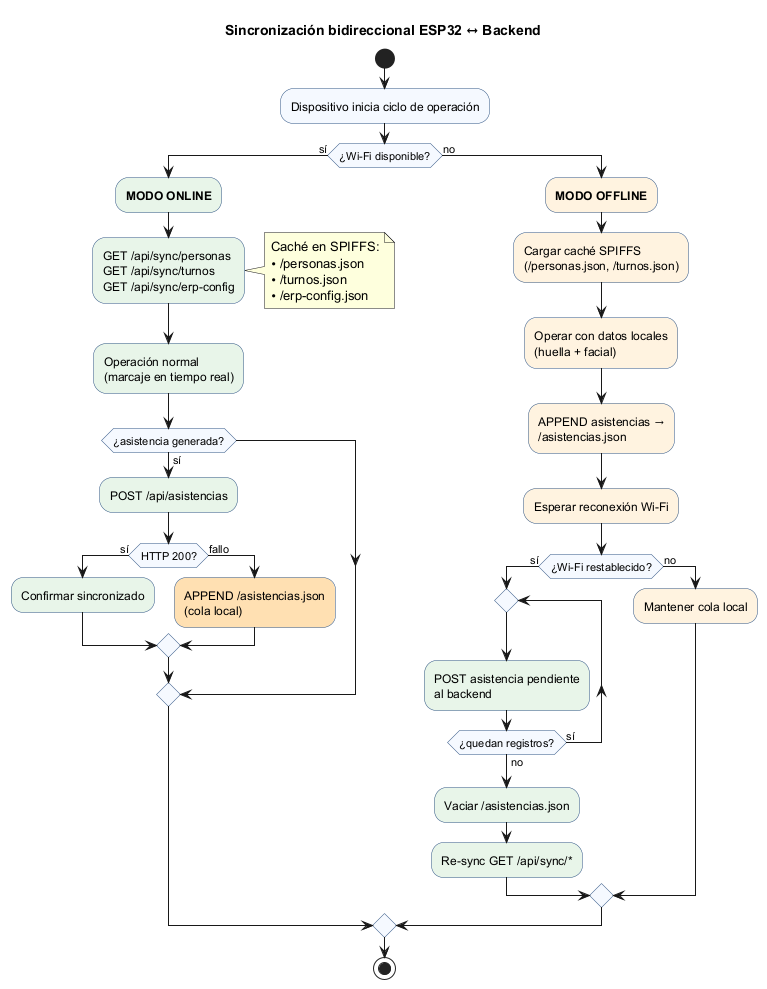
\includegraphics[width=0.95\linewidth]{diagrams/flujo_sincronizacion_bidireccional.png}
  \caption{Diagrama de actividad: sincronización bidireccional entre los modos online y offline del ESP32-CAM.}
  \label{fig:flujo_sync}
\end{figure}

\paragraph{Deduplicación en el backend}

El endpoint POST /api/asistencias/sync implementa una verificación previa a la inserción: para cada registro del lote, consulta si ya existe una asistencia de la misma persona (persona\_id), mismo tipo (entrada/salida), mismo turno\_id y misma fecha (DATE(fecha\_hora) = CURRENT\_DATE). Si existe, omite la inserción. Esta verificación por turno\_id permite que un trabajador registre múltiples asistencias en un mismo día si pertenece a distintos turnos (por ejemplo, jornada diurna y jornada nocturna), sin generar duplicados dentro del mismo turno. Garantiza idempotencia ante reenvíos.

\paragraph{Tablas de auditoría}

\begin{itemize}
    \item sincronizacion\_log: Registra cada operación de sincronización con: dispositivo de origen, cantidad de registros enviados, cantidad procesada correctamente, estado y detalle.
    \item logs\_biometricos: Registra cada operación biométrica con: persona, dispositivo, timestamp, tipo de operación (registro, verificación, identificación), resultado (éxito, fallo, duplicado, no\_encontrado) e IP de origen.
    \item eliminaciones\_biometricas: Registra cada eliminación de datos biométricos con: persona, embedding anterior (cifrado), ruta de la foto eliminada y usuario solicitante.
\end{itemize}

\paragraph{Panel de visualización de logs}

El backend expone dos conjuntos de endpoints para consulta de logs:
\begin{itemize}
    \item GET /api/logs: Lista los registros de sincronización, con filtro por empresa para roles no-admin.
    \item DELETE /api/logs: Permite limpiar los logs (admin limpia todo, empleador limpia los de su empresa).
    \item El ESP32-CAM expone GET /api/logs que retorna el buffer de logs en formato HTML, y /api/logs/clear para limpiarlo.
\end{itemize}

\paragraph{Script de simulación de asistencia facial}

Se desarrolló deteccion.py, un script de línea de comandos que permite probar el flujo de reconocimiento facial sin necesidad del ESP32-CAM. El script escanea las fotos almacenadas localmente para el ambiente de pruebas, presenta un menú interactivo para seleccionar una de ellas, ejecuta el proceso de identificación 1:N contra la base de datos y registra la asistencia correspondiente. Es útil para pruebas de regresión rápida y demostraciones.

\subsubsection{Implementación}

\paragraph{Sincronización en el ESP32-CAM}

Las funciones de sincronización siguen un patrón común:

\begin{enumerate}
    \item Verificar conectividad (isOnline y WiFi.status() == WL\_CONNECTED).
    \item Cargar los datos locales desde LittleFS.
    \item Iterar sobre los registros con sincronizado = false.
    \item Para cada uno, construir el payload JSON y enviarlo al backend vía HTTP POST.
    \item Si el backend responde con éxito (HTTP 200/201), marcar sincronizado = true y actualizar el backend\_id si corresponde.
    \item Persistir los cambios en LittleFS.
\end{enumerate}

Para las personas, además del envío de pendientes, se implementa la descarga completa desde el backend (sincronizarPersonasDesdeBackend()) que sobrescribe el archivo local si no hay registros locales pendientes, manteniendo el ESP32-CAM actualizado con los datos del servidor.

\paragraph{Campo colación en turnos}

Los turnos incorporaron los campos con\_colacion (booleano), colacion\_inicio (TIME) y colacion\_fin (TIME) para modelar el horario de colación de los trabajadores, en cumplimiento del artículo 34 del Código del Trabajo chileno. En la tabla turnos de PostgreSQL se almacenan como TIME (o NULL si con\_colacion = FALSE). Los endpoints CRUD de routes/turnos.py gestionan estos campos: al crear un turno, se envían con\_colacion, colacion\_inicio y colacion\_fin; al actualizar, se usa COALESCE para preservar valores existentes si no se envían. Las consultas GET retornan los horarios como string o null según corresponda. El campo turno\_id se agregó también a la tabla asistencias para asociar cada marcación al turno bajo el cual se registró, permitiendo el cálculo preciso de horas trabajadas descontando la colación.

\paragraph{Sincronización de asistencias por lote}

La función sincronizarAsistencias() en el ESP32-CAM es especialmente relevante porque maneja el caso más frecuente de datos offline: un trabajador marcó entrada y salida durante el día sin conexión. La función:

\begin{enumerate}
    \item Carga asistencias.json y filtra las que tengan sincronizado = false.
    \item Construye un JSON con estructura \{"registros": [...]\}.
    \item Lo envía a POST /api/asistencias/sync.
    \item Si el backend retorna HTTP 200, marca todos los registros enviados como sincronizados.
\end{enumerate}

\paragraph{Sincronización en el backend}

El endpoint POST /api/asistencias/sync en routes/asistencias.py recibe el lote e itera sobre cada registro, aplicando la verificación de duplicados y realizando la inserción. También dispara el envío a ERP para cada asistencia nueva.

\paragraph{Watchdog y ping activo de dispositivos}

La detección de desconexión de dispositivos se implementó con tres capas complementarias:

\begin{enumerate}
    \item \textbf{LWT (instantáneo)}: Al conectarse al broker MQTT, el ESP32-CAM configura un mensaje Last Will en esp32/lwt/<MAC>. Si el dispositivo se desconecta abruptamente, el broker publica automáticamente el LWT y el backend marca el dispositivo como inactivo de inmediato.
    \item \textbf{Ping activo (device\_pinger)}: Un hilo separado publica periódicamente (cada 30 segundos) un mensaje en el tópico esp32/ping/<MAC>. El ESP32-CAM, al recibirlo, responde publicando un heartbeat con el campo "pong": true. Si el backend no recibe respuesta dentro de 60 segundos, marca el dispositivo como inactivo. Este mecanismo funciona incluso si el mensaje LWT no fue entregado.
    \item \textbf{Watchdog pasivo (device\_watchdog)}: Un hilo ejecutado cada 60 segundos realiza un barrido inicial al arrancar el backend (todos los dispositivos se marcan inactivo) y luego verifica periódicamente qué dispositivos no han enviado heartbeat en más de 90 segundos, marcándolos como inactivos.
\end{enumerate}

Esta arquitectura de tres capas asegura que ninguna desconexión pase desapercibida: el LWT atrapa las desconexiones abruptas detectadas por el broker; el ping activo detecta silencios de red donde el LWT no alcanza a publicarse; y el watchdog pasivo actúa como respaldo final para cualquier caso no cubierto por las capas anteriores.

\paragraph{Herramienta de simulación facial}

Como complemento durante el desarrollo se implementó deteccion.py, un script de línea de comandos que permitió probar el flujo de reconocimiento facial sin necesidad del ESP32-CAM. El script se conectaba directamente a PostgreSQL, ejecutaba DeepFace (Facenet + detector configurable + anti-spoofing) sobre imágenes almacenadas localmente para el ambiente de pruebas, y registraba asistencias de prueba en la base de datos. En las etapas finales del proyecto, esta funcionalidad de simulación fue absorbida por la suite de pruebas automatizadas (con mocks de DeepFace, OpenCV y PostgreSQL en Docker), que ofrece mayor repetibilidad y cobertura sin dependencia del sistema de archivos local.

\paragraph{Flujo operacional consolidado}
\label{sec:flujo_operacional_consolidado}

Con todos los componentes del sistema ya construidos (enrolamiento por PIN, reconocimiento biométrico, almacenamiento offline, sincronización diferida e integración ERP), la Fig.~\ref{fig:flujo_operacional} consolida el camino completo que sigue una marcación, cubriendo tanto el caso con conexión a internet como el caso sin ella, tal como quedó implementado al cierre del proyecto.

El flujo comienza cuando el sensor PIR detecta presencia frente al dispositivo y se ejecuta la captura biométrica (huella mediante el AS608 o rostro mediante la cámara OV2640). A partir de ahí, el firmware evalúa isCloudReady(): si el dispositivo está conectado a internet y enrolado, la marcación se envía de inmediato al backend por HTTP (POST /api/facial/identificar para rostro, o POST /api/asistencias para huella). Si cualquiera de esas dos condiciones falla, la marcación se guarda localmente en asistencias.json (LittleFS) con la marca sincronizado=false, se muestra el resultado en el panel embebido sin esperar respuesta del servidor, y el dispositivo queda a la espera de que la conexión se restablezca para ejecutar sincronizarPendientes(), que vacía la cola completa hacia el backend.

Ambos caminos, el envío inmediato y la sincronización diferida, terminan convergiendo en el mismo punto: el backend valida la huella o el rostro contra los registros almacenados (encodings\_faciales o el identificador de huella) y persiste el resultado en la tabla asistencias de PostgreSQL. Si la identificación es exitosa, el backend responde 200 OK, dispara en un hilo aparte el envío hacia los sistemas ERP configurados, y el firmware ejecuta flashExito(), que hace parpadear el LED verde del dispositivo dos veces. Si no hay coincidencia o la imagen no cumple el filtro de calidad, el backend responde con un código de error (404 o 400) y la operación queda registrada en logs\_biometricos para su auditoría posterior; en este caso el firmware invoca flashError(), una función que existe en el código como punto de extensión para una señal de error distinta, pero que actualmente no tiene ninguna acción implementada.

\begin{figure}[H]
    \centering
    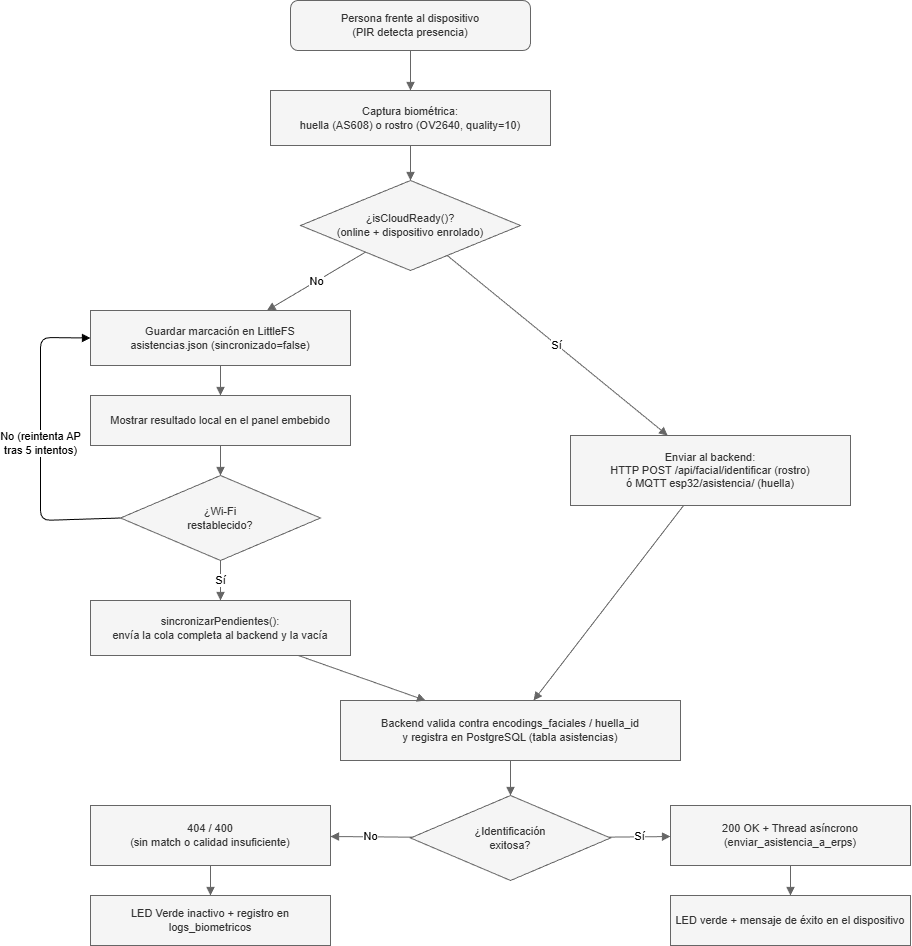
\includegraphics[width=.85\linewidth]{Imagenes/flujo_operacional_asistencia.png}
    \caption{Flujo operacional consolidado para el registro de asistencia.}
    \label{fig:flujo_operacional}
\end{figure}

\subsubsection{Pruebas}
\label{sec:pruebas_unitarias_automatizadas}

Se diseñaron las siguientes pruebas para validar la sincronización diferida, los logs y la integración final:

\begin{itemize}
    \item \textbf{Prueba de sincronización de asistencias offline}: Desconectar el ESP32-CAM de la red, registrar 5 marcaciones de entrada/salida para 2 personas diferentes, reconectar y ejecutar sincronización. Verificar que los 5 registros aparezcan en la base de datos del backend y que el archivo asistencias.json local los marque como sincronizados.

    \item \textbf{Prueba de idempotencia de sincronización}: Tras una sincronización exitosa, ejecutar nuevamente la sincronización sin nuevos registros. Verificar que no se inserten registros duplicados en el backend.

    \item \textbf{Prueba de sincronización de personas creadas offline}: Desconectar el dispositivo, registrar una nueva persona (con huella y datos), reconectar y sincronizar. Verificar que la persona aparezca en el backend con un ID definitivo (no local-).

    \item \textbf{Prueba de sincronización de turnos y asignaciones}: Desconectar el dispositivo, crear un turno y asignarlo a una persona existente, reconectar y sincronizar. Verificar que el turno y la asignación se repliquen en el backend y que los backend\_id locales se actualicen correctamente.

    \item \textbf{Prueba de persistencia tras corte de energía}: Durante una sincronización en curso, cortar la alimentación del ESP32-CAM. Al reiniciar, verificar que los archivos JSON no estén corruptos y que los registros con sincronizado = false sigan estando disponibles para una nueva sincronización.

    \item \textbf{Prueba de duplicados por turno}: Registrar dos asistencias con la misma persona, tipo, turno y fecha. Verificar que el sistema rechace la segunda inserción por duplicado. Registrar asistencias con diferentes turno\_id para un mismo día y verificar que ambas se registren sin conflictos.

    \item \textbf{Prueba de colación en turnos}: Crear un turno con colación habilitada (con\_colación = true) especificando horario de colación. Verificar que los campos colacion\_inicio y colacion\_fin se almacenen correctamente como TIME en la base de datos. Crear un turno sin colación y verificar que ambos campos sean NULL.

    \item \textbf{Prueba de logs de sincronización}: Ejecutar 3 sincronizaciones con diferentes cantidades de registros. Verificar que en la tabla sincronizacion\_log del backend aparezcan 3 entradas con los conteos correctos de registros enviados y procesados.

    \item \textbf{Prueba de logs biométricos}: Realizar operaciones de registro facial, identificación exitosa, identificación fallida y verificación. Verificar que cada operación genere una entrada en logs\_biometricos con el tipo de operación y resultado correctos.

    \item \textbf{Prueba de watchdog}: Iniciar el backend, verificar que todos los dispositivos se marquen como inactivos. Conectar un ESP32-CAM, verificar que tras el primer heartbeat cambie a activo. Desconectar el ESP32-CAM y verificar que tras 90 segundos el watchdog lo marque como inactivo.

    \item \textbf{Prueba de ping activo}: Conectar un ESP32-CAM, verificar que el backend publique pings en esp32/ping/<MAC> y que el dispositivo responda. Detener el ESP32-CAM (corte de red) y verificar que el ping activo marque el dispositivo como inactivo antes de que el watchdog de 90 segundos actúe (tiempo de espera de 60 segundos).

    \item \textbf{Prueba de simulación facial automatizada}: Utilizar la suite de pruebas test\_routes\_facial.py y el emulador test\_identificacion\_facial.py para simular el flujo completo de identificación 1:N con imágenes sintéticas generadas en memoria, cubriendo casos de coincidencia exitosa, rostro no registrado y calidad insuficiente de imagen.

    \item \textbf{Prueba de flujo completo punta a punta}: Ejecutar el flujo completo: registrar persona con huella y rostro en el ESP32-CAM $\rightarrow$ sincronizar con backend $\rightarrow$ verificar que la persona aparezca en el panel web $\rightarrow$ marcar asistencia por huella offline $\rightarrow$ reconectar y sincronizar $\rightarrow$ verificar que la asistencia aparezca en el panel web y se envíe al ERP de prueba.
\end{itemize}

\paragraph{Pruebas automatizadas}

Además de las pruebas funcionales descritas, se implementó una suite de más de 590 pruebas automatizadas para el backend y el firmware, utilizando pytest con PostgreSQL en Docker y mocks para DeepFace, OpenCV y MQTT. La suite se organiza en 35 archivos de prueba y alcanza una cobertura de código del 98\% sobre el código de producción del backend, sin fallos en ninguna de las pruebas (ver Anexo D para el detalle de casos y la evolución de la cobertura por módulo). La integración con los ERP externos se valida en dos niveles: por un lado, las pruebas de la suite automatizada cubren la creación, edición y prueba de webhooks de una integración ERP, simulando la respuesta del servidor externo. Por otro lado, dentro del subdirectorio ERPSIMULATORS/ se construyeron tres simuladores independientes (mock\_odoo.py, mock\_defontana.py y mock\_buk.py), cada uno levantando un pequeño servidor Flask que reproduce los endpoints reales de autenticación, consulta de empleados e inyección de marcaciones de su respectivo ERP comercial, según la documentación pública de cada proveedor. El script test\_erp\_mocks.py se ejecuta por separado, con los tres simuladores corriendo: envía una marcación con el formato que genera el sistema hacia cada uno de los tres mocks y verifica que el field mapping configurado para cada ERP transforme correctamente los datos y que cada simulador responda como lo haría el sistema real, imprimiendo un reporte de éxito o falla por caso. Esta validación manual complementa, sin sustituir, a las pruebas automatizadas de pytest.

Las pruebas cubren los flujos de todas las iteraciones: inicialización de la aplicación, esquema de base de datos, cifrado de embeddings, servicio de correo electrónico (con mock de SMTP), handlers MQTT, autenticación JWT con roles jerárquicos y flujo multi-empresa, endpoints faciales, CRUD de personas/turnos/asignaciones/asistencias, verificación de dispositivos, integraciones ERP con tolerancia a fallos de conexión y timeout, enrolamiento de dispositivos mediante PIN, sincronización offline, y logs de auditoría. Entre los módulos con mayor cobertura destacan el cifrado de embeddings (100\%), el servicio de correo (100\%), la gestión de turnos (100\%), la base de datos (99\%) y el módulo de asignaciones (96\%). El detalle completo de los casos de prueba se incluye en el Anexo D, que además resume los resultados obtenidos al ejecutar la suite completa.

\subsubsection{Refinamientos posteriores}

\begin{itemize}
    \item \textbf{Limpieza de datos al eliminar una persona}: el endpoint de eliminación distingue dos comportamientos según el rol de quien lo invoca. Un administrador ejecuta una limpieza completa de datos biométricos y sensibles: anonimiza el RUT, el correo y el identificador de huella, elimina los encodings\_faciales y los consentimientos asociados, borra la foto de previsualización del disco y marca a la persona como inactiva, conservando únicamente su historial de asistencias. Un empleador, en cambio, solo puede marcar a la persona como inactiva, sin acceso a la limpieza de datos biométricos, reservada al rol con mayor privilegio.

    \item \textbf{Filtro activo = true en los listados}: todas las consultas de lectura sobre personas (y entidades equivalentes) incorporan la condición WHERE activo = true, de modo que los registros eliminados mediante soft-delete dejan de aparecer en listados y búsquedas sin perder su información histórica en la base de datos, requisito necesario para mantener la integridad de los reportes de asistencia ya generados.
\end{itemize}


\section{Mecanismos de seguridad}

Esta sección consolida los mecanismos de seguridad implementados a lo largo de las distintas iteraciones, descritos en su momento dentro del desarrollo de cada una (Secciones 4.2.3 a 4.2.5), agrupándolos por capa: autenticación y control de acceso, enrolamiento de dispositivos, y protección de datos biométricos.

\subsection{Autenticación y control de acceso}

El backend define tres decoradores de autenticación en routes/auth.py, aplicados según el tipo de cliente que consume cada endpoint:

\begin{itemize}
    \item @token\_required: exige un header Authorization: Bearer <token> con un JWT firmado con el algoritmo HS256 y una clave secreta (JWT\_SECRET, configurable por variable de entorno). El token incluye user\_id, empresa\_id, rol y, opcionalmente, persona\_id, con una expiración de 24 horas. Si el token falta, está expirado o es inválido, el endpoint responde con HTTP 401.

    \item @requiere\_rol(*roles): envuelve a @token\_required y además exige que request.user\_rol esté dentro de los roles permitidos (admin, empleador o trabajador), respondiendo HTTP 403 en caso contrario. Implementa así un control de acceso jerárquico basado en roles sobre los mismos endpoints autenticados.

    \item @token\_opcional: permite que un mismo endpoint sea consumido tanto por un cliente web autenticado con JWT como por un dispositivo ESP32-CAM identificado mediante el header X-Device-MAC. Si no hay JWT, el decorador busca la MAC recibida entre los dispositivos ya enrolados y, de encontrarla, expone request.dispositivo\_id y request.empresa\_id para el resto del endpoint. Como se detalla en la Sección 4.2.5, este decorador ya no crea dispositivos nuevos automáticamente: solo vincula los que ya pasaron por el flujo de enrolamiento con PIN.

    \item @requiere\_dispositivo\_enrolado: complementa a @token\_opcional en endpoints biométricos sensibles (por ejemplo, /api/facial/registrar), verificando explícitamente que el dispositivo de la petición tenga enrolado = TRUE en la base de datos antes de continuar, y respondiendo HTTP 403 en caso contrario.
\end{itemize}

Las contraseñas de los usuarios del panel web nunca se almacenan en texto plano: se procesan con bcrypt \cite{bcrypt_pypi} (función hashpw con sal generada por gensalt()) tanto al crear una cuenta como al cambiar la contraseña, y la verificación en el login usa bcrypt.checkpw para comparar contra el hash almacenado.

\subsection{Enrolamiento seguro de dispositivos}

Un dispositivo ESP32-CAM no puede operar contra el backend simplemente conectándose a la red: debe pasar por un flujo de enrolamiento explícito basado en un PIN de un solo uso. Un administrador o empleador solicita POST /api/auth/dispositivos/generar-pin, que crea en la base de datos un registro en dispositivos con enrolado = FALSE y un código aleatorio de 8 caracteres alfanuméricos (generado con el módulo secrets, criptográficamente seguro). El dispositivo, desde su panel de configuración Wi-Fi, envía ese PIN junto con su dirección MAC al backend; si el PIN es válido y no fue usado antes, el dispositivo queda marcado como enrolado = TRUE y asociado a la MAC y a la empresa que generó el PIN. Un PIN ya consumido no puede reutilizarse (HTTP 409).

En el firmware, la función isCloudReady() (Sección 4.2.1) actúa como una verificación de doble factor antes de cualquier operación dependiente del backend: exige tanto conectividad de red (isOnline) como enrolamiento confirmado (estaEnrolado), evitando que un dispositivo conectado pero no autorizado, o autorizado pero sin red, ejecute operaciones que comprometerían la consistencia del sistema.

\subsection{Protección de datos biométricos}

Los embeddings faciales generados por DeepFace se cifran antes de almacenarse en la base de datos mediante Fernet (AES-128 en modo CBC con autenticación HMAC-SHA256), de la librería cryptography de Python. La clave de cifrado no se almacena directamente: se deriva aplicando SHA-256 a una variable de entorno (BIOMETRIC\_KEY) y codificando el resultado en base64 URL-safe, tal como lo exige la API de Fernet:

\begin{verbatim}
def _derivar_fernet_key() -> bytes:
    digest = hashlib.sha256(BIOMETRIC_KEY.encode("utf-8")).digest()
    return base64.urlsafe_b64encode(digest)
\end{verbatim}

De esta forma, ni el embedding ni la clave de cifrado quedan expuestos en texto plano en la base de datos: un acceso no autorizado a las tablas encodings\_faciales solo expone valores cifrados, mientras la clave reside exclusivamente en la configuración del entorno de ejecución del backend.

\section{Arquitectura de tiempo real (SSE)}

El panel web necesita reflejar, sin recargar la página, el estado de conexión de cada ESP32-CAM y el progreso del enrolamiento de huellas. Esta sección consolida cómo se implementó esa capa de tiempo real, descrita parcialmente al introducirse en las iteraciones 3 y 7 (Secciones 4.2.3 y 4.2.5).

\subsection{Endpoints de streaming}

El backend expone dos endpoints SSE (Server-Sent Events) implementados en app.py con el patrón estándar de Flask para streaming: una función generadora que produce eventos en formato text/event-stream, devuelta mediante Response(stream\_with\_context(generate()), mimetype='text/event-stream').

\begin{itemize}
    \item GET /sse/devices: difunde, a todos los clientes conectados, los cambios de estado de los dispositivos (heartbeat recibido, LWT disparado, ping sin respuesta), mediante la función broadcast\_device\_update().
    \item GET /sse/huellas: difunde el resultado del enrolamiento de huellas recibido por MQTT en esp32/huella/resultado/\#, mediante broadcast\_huella\_update(), permitiendo que el panel muestre en vivo el progreso del registro biométrico.
\end{itemize}

Se optó por SSE porque el caso de uso es unidireccional (servidor a cliente) y se consume en el navegador con la API nativa EventSource, sin depender de librerías adicionales en el frontend ni de un protocolo de negociación propio como el de WebSockets.

\subsection{Tres capas de detección de desconexión}

Determinar si un ESP32-CAM sigue conectado es más complejo que solo esperar sus heartbeats, porque una caída de red puede impedir que el dispositivo avise que se desconectó. El backend combina tres mecanismos complementarios, implementados en mqtt\_handler.py:

\begin{enumerate}
    \item \textbf{LWT (Last Will and Testament)}: al conectarse al broker MQTT, el ESP32-CAM registra un mensaje LWT en esp32/lwt/<MAC>. Si la conexión TCP se rompe de forma anómala (corte de energía, pérdida abrupta de señal), el propio broker Mosquitto publica ese mensaje automáticamente, sin que el backend tenga que esperar ningún timeout. Es la capa más rápida, pero depende de que el broker detecte la caída de la conexión subyacente.

    \item \textbf{Ping activo (device\_pinger)}: un hilo en segundo plano publica, cada 30 segundos, un mensaje en esp32/ping/<MAC> para cada dispositivo enrolado. El ESP32-CAM responde con un heartbeat normal al recibirlo. Si un dispositivo no responde dentro de la ventana definida por HEARTBEAT\_TIMEOUT (60 segundos), el pinger lo marca como inactivo directamente, sin esperar al watchdog. Esta capa cubre los casos en que el LWT no llega a publicarse (por ejemplo, si el broker tampoco detecta la caída).

    \item \textbf{Watchdog pasivo (device\_watchdog)}: un segundo hilo revisa cada 60 segundos la antigüedad del último heartbeat de cada dispositivo y marca como inactivos a los que superan los 60 segundos sin responder. Actúa como respaldo final, independiente del pinger, y además ejecuta un barrido inicial al arrancar el backend que marca a todos los dispositivos como inactivos hasta recibir su primer heartbeat.
\end{enumerate}

Cada vez que cualquiera de estas tres capas cambia el estado de un dispositivo en la base de datos, invoca broadcast\_device\_update(), que propaga el cambio de inmediato a los clientes SSE conectados.

\subsection{Consumo en el frontend}

En el panel web (Next.js), un hook personalizado se conecta directamente al endpoint /sse/devices mediante EventSource, actualizando en memoria el estado, IP y último heartbeat de cada dispositivo a medida que llegan eventos, sin necesidad de refrescar la página ni de mantener una conexión WebSocket. Como mecanismo de respaldo ante una eventual interrupción de la conexión SSE, el frontend además consulta periódicamente GET /api/dispositivos por REST, de modo que el estado mostrado no depende exclusivamente del canal de streaming.

\section{Prototipo final}
\label{sec:prototipo_final}

Esta sección presenta el resultado físico del proceso de desarrollo descrito en las ocho iteraciones anteriores, mostrando el dispositivo ESP32-CAM ensamblado junto con sus componentes periféricos (cámara OV2640, lector de huellas AS608 y sensor PIR), así como el panel web resultante.

%% Reemplazar por las fotografías reales del prototipo final.
%% Se recomienda incluir: (1) vista general del dispositivo ensamblado,
%% (2) detalle de conexiones/componentes, (3) dispositivo en su carcasa/montaje final,
%% (4) captura del panel web administrativo en funcionamiento.

\begin{figure}[H]
  \centering
  \includegraphics[width=0.75\linewidth]{Imagenes/prototipo_final_1.jpg}
  \caption{Vista general del prototipo final ensamblado.}
  \label{fig:prototipo_final_1}
\end{figure}

\begin{figure}[H]
  \centering
  \includegraphics[width=0.75\linewidth]{Imagenes/prototipo_final_2.jpg}
  \caption{Detalle de los componentes del prototipo: cámara OV2640, lector de huellas AS608 y sensor PIR.}
  \label{fig:prototipo_final_2}
\end{figure}

\begin{figure}[H]
  \centering
  \includegraphics[width=0.75\linewidth]{Imagenes/prototipo_final_3.jpg}
  \caption{Prototipo final montado en su carcasa definitiva.}
  \label{fig:prototipo_final_3}
\end{figure}

\begin{figure}[H]
  \centering
  \includegraphics[width=0.9\linewidth]{Imagenes/prototipo_final_4.jpg}
  \caption{Panel web administrativo en funcionamiento durante una prueba de campo.}
  \label{fig:prototipo_final_4}
\end{figure}

%% ============================================================
\section{Resumen del capítulo}
El capítulo 4 presenta el desarrollo completo del prototipo a lo largo de ocho iteraciones, siguiendo la metodología de prototipado evolutivo incremental. Se documenta la integración del hardware (ESP32-CAM, lector AS608, sensor PIR, cámara OV2640), la implementación del almacenamiento local con LittleFS y JSON, el desarrollo del backend con Flask y PostgreSQL (14 tablas con soporte multi-tenant), la comunicación mediante HTTP y MQTT, el reconocimiento facial con DeepFace (modelo Facenet, detector configurable MTCNN/RetinaFace y anti-spoofing), el cifrado de embeddings biométricos con Fernet, la autenticación JWT con roles jerárquicos, el enrolamiento seguro de dispositivos mediante PIN, el sistema antifraude multicapa (PIR + flash PWM + anti-spoofing + cooldown), el panel web para la gestión del dispositivo con streaming SSE de estado en tiempo real, la integración con ERP externos vía webhooks con field mapping, los mecanismos de sincronización diferida con logs de auditoría, y la detección de desconexión mediante un sistema de tres capas (LWT, ping activo y watchdog pasivo).

Cada iteración incluyó su respectivo análisis de requisitos, diseño de la solución, implementación detallada y un plan de pruebas de integración para validar el correcto funcionamiento de los componentes desarrollados. Adicionalmente, se documenta la suite de 591 pruebas unitarias automatizadas con pytest, que alcanzó una cobertura de código del 98\% sobre las 3.382 líneas de producción del backend, incluyendo pruebas de caja negra sobre los endpoints de la API REST y verificación exhaustiva de todos los caminos de error.

El Anexo C presenta, mediante diagramas de actividades, las principales funcionalidades implementadas en el sistema: el enrolamiento de dispositivos (Figura~\ref{fig:flujo_enrolamiento_dispositivo}), el registro de personas y captura biométrica (Figura~\ref{fig:flujo_registro_personas}), la gestión de turnos y su asignación (Figura~\ref{fig:flujo_gestion_turnos}), la sincronización diferida de asistencias pendientes (Figura~\ref{fig:flujo_sincronizacion_pendientes}) y el panel web administrativo (Figura~\ref{fig:flujo_panel_administrativo}). en memoria.tex
%% ============================================================

\chapter{Desarrollo e implementación}
En el siguiente capítulo se presentan en detalle las 8 iteraciones del proyecto, desarrolladas según la metodología de prototipado evolutivo incremental descrita en el capítulo 3. Para cada iteración se describen las fases de análisis, diseño, implementación y pruebas, reflejando la construcción progresiva del prototipo desde la integración inicial de hardware hasta la sincronización diferida y el cierre del proyecto.

\section{Diseño de software}
Esta sección está destinada a presentar las arquitecturas desarrolladas para este proyecto como así diagramas y mockups que permitan dar entender la lógica del proyecto como así futuras vistas.

\subsection{Arquitectura física}
La arquitectura física se organiza como un conjunto de servicios independientes que se comunican entre sí, siguiendo un enfoque de microservicios. La Fig.~\ref{fig:arq_fisica} muestra los componentes físicos involucrados y el camino que recorre una marcación desde que se genera hasta que queda disponible para la empresa: el ESP32-CAM, como dispositivo de campo, captura la imagen o la huella y la envía hacia el servidor mediante el broker MQTT (Mosquitto) o vía HTTP, según el tipo de operación. El backend (Flask) recibe esa información, invoca al servicio de reconocimiento facial (DeepFace) cuando corresponde, y persiste el resultado en la base de datos PostgreSQL. Desde ahí, el mismo backend se encarga de dos salidas independientes: reenviar la marcación al sistema ERP de la empresa mediante un webhook, y exponerla en el panel web (Next.js) para que el administrador o empleador la consulte en tiempo real.

\begin{figure}[H]
  \centering
  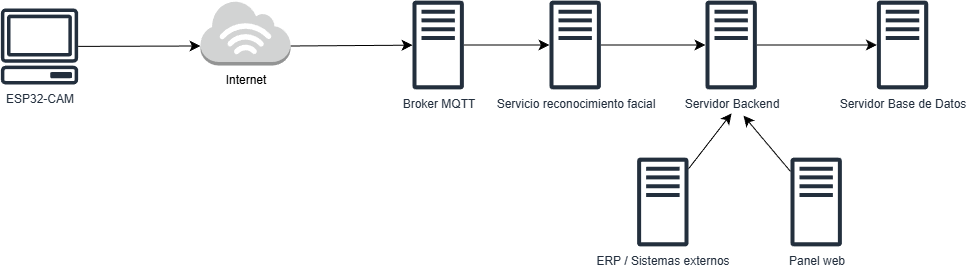
\includegraphics[width=\linewidth]{Imagenes/arqui2.drawio.png}
  \caption{Arquitectura física.}
  \label{fig:arq_fisica}
\end{figure}

\subsection{Arquitectura lógica}
Mientras que la arquitectura física muestra dónde corre cada servicio, la arquitectura lógica de la Fig.~\ref{fig:arq_logica} muestra cómo se organizan los módulos de software dentro de esos servicios y cómo se relacionan entre sí. En el lado del dispositivo, el ESP32-CAM agrupa cuatro módulos: la captura de imágenes (cámara OV2640), la lectura de huella (lector AS608 vía UART), el almacenamiento local en LittleFS (usuarios, turnos, asignaciones y asistencias en formato JSON) y el servidor web embebido que sirve la interfaz de configuración. Estos cuatro módulos no son independientes entre sí: por ejemplo, una marcación capturada por la cámara o el lector se guarda primero en LittleFS y solo después se intenta enviar al backend, lo que permite que el dispositivo siga funcionando aunque no haya conexión.

Del lado del servidor, el backend se organiza en blueprints de Flask (uno por dominio: personas, turnos, asistencias, dispositivos, ERP, etc.), cada uno con acceso a la base de datos PostgreSQL y, cuando corresponde, al servicio de reconocimiento facial. La comunicación entre el dispositivo y el backend ocurre por dos canales según el tipo de mensaje: MQTT para eventos de bajo volumen (heartbeats, comandos, resultados de enrolamiento) y HTTP para el envío de imágenes y la sincronización de datos. Esta separación de canales es la que permite que el dispositivo opere de forma autónoma cuando no hay red, almacene localmente lo que no pudo enviar, y sincronice todo una vez que la conexión se restablece.

\begin{figure}[H]
  \centering
  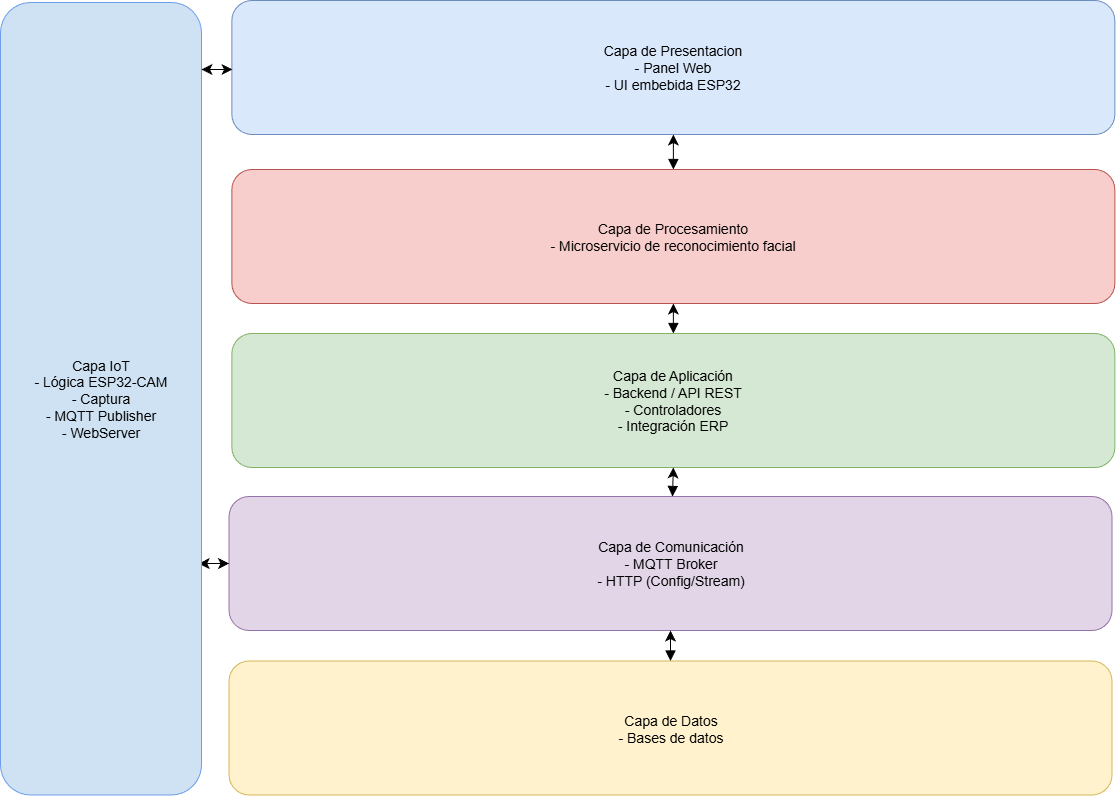
\includegraphics[width=.75\linewidth]{Imagenes/arquilogica.png}
  \caption{Arquitectura lógica.}
  \label{fig:arq_logica}
\end{figure}

La Fig.~\ref{fig:componentes_esp32} detalla, a nivel de hardware y firmware, los mismos cuatro módulos del ESP32-CAM descritos en la arquitectura lógica. En la capa de hardware se distinguen el microcontrolador ESP32, la cámara OV2640 (conectada por el bus paralelo DVP), el lector de huellas AS608 (conectado por UART) y el sensor PIR que activa la captura solo ante presencia detectada. En la capa de firmware, el servidor web embebido y el cliente MQTT comparten el acceso al sistema de archivos LittleFS, mientras que la máquina de estados central coordina cuándo se invoca cada módulo de captura biométrica según si el dispositivo está en modo de registro o de marcaje. Esta vista complementa a la Fig.~\ref{fig:arq_logica}, mostrando con qué pines y protocolos concretos se implementa cada bloque lógico.

\begin{figure}[H]
  \centering
  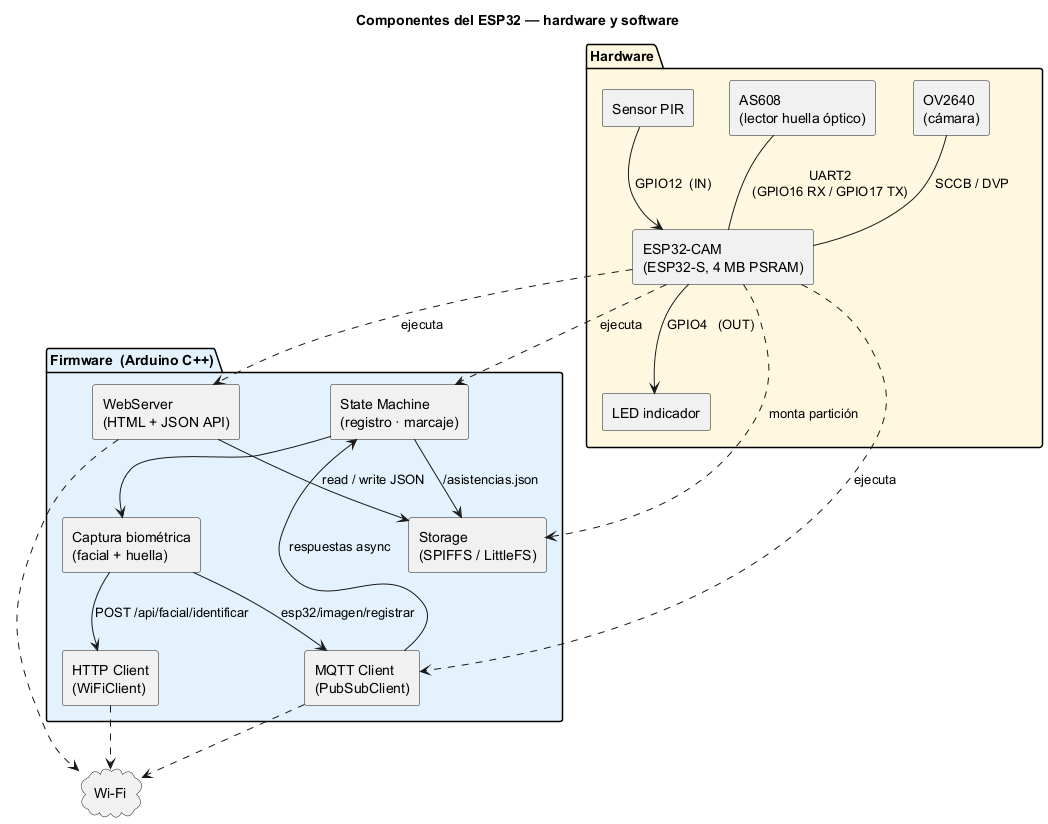
\includegraphics[width=\linewidth]{diagrams/componentes_esp32.png}
  \caption{Componentes del ESP32-CAM: hardware y firmware.}
  \label{fig:componentes_esp32}
\end{figure}

\section{Implementación}

En este apartado se procederá a explicar cómo se llevaron a cabo las iteraciones planteadas en el capítulo 3.1.

%% ============================================================
%% ITERACIÓN 1: Diseño y planificación inicial
%% ============================================================
\subsection{Iteración 1: Integración de hardware y servidor embebido}

La primera iteración corresponde al diseño conceptual del sistema y a la preparación del entorno de desarrollo, incluyendo la integración inicial del hardware biométrico seleccionado. Esta etapa establece la base funcional sobre la cual se construirán las iteraciones posteriores.

\subsubsection{Análisis}

En esta iteración se definieron los requisitos mínimos para validar la viabilidad técnica del sistema, analizando los componentes del hardware y las funcionalidades necesarias para las iteraciones siguientes.

El análisis se centró en tres ejes principales:

\begin{itemize}
    \item \textbf{Definición de funcionalidades mínimas (MVP)}:  
    Se identificaron las capacidades básicas que el dispositivo debía cumplir desde el inicio: capturar imágenes desde la cámara integrada, leer huellas dactilares mediante el sensor AS608, montar un servidor HTTP local con páginas HTML embebidas y operar de forma autónoma mediante Wi-Fi. Estas funciones representan la base operativa sobre la cual se desarrollarán características más avanzadas como turnos, sincronización y gestión de usuarios.

    \item \textbf{Identificación de limitaciones técnicas}:  
    Se revisaron las restricciones tecnológicas del ESP32-CAM, como la limitada memoria RAM disponible (~520 KB), el uso compartido del bus de cámara con los pines GPIO, la ausencia de pines GPIO libres -lo que forzó el uso de los pines GPIO14 (RX) y GPIO15 (TX) para la comunicación UART con el lector de huellas- y la necesidad de un manejo eficiente de cadenas HTML grandes en memoria. También se identificó que el flash LED integrado consume corriente significativa (~250 mA), requiriendo protección mediante PWM para evitar caídas de tensión durante la captura.

    \item \textbf{Estrategia de operación autónoma}:  
    Dado que uno de los requisitos fundamentales del sistema es la autonomía, se analizó la necesidad de montar un servidor web local. En caso de no contar con Wi-Fi configurada, el dispositivo debe activar automáticamente un modo Access Point (AP) con SSID ESP32-ASISTENCIA, permitiendo al administrador conectarse directamente para configurar la red y registrar usuarios sin dependencia de internet. Esto reduce riesgos y asegura la continuidad operacional del dispositivo.
\end{itemize}

Como resultado del análisis, se establecieron los criterios de diseño que guiarían el desarrollo de esta iteración: simplicidad, bajo consumo de recursos, modularidad de componentes y autonomía operativa.

\subsubsection{Diseño}

En esta iteración se elaboraron los primeros elementos arquitectónicos del sistema:

\begin{itemize}
    \item \textbf{Arquitectura física}, representando los componentes utilizados y su interconexión, la cual se puede revisar en la Fig.~\ref{fig:arq_fisica} de la sección 4.1.1.

    \item \textbf{Arquitectura lógica}, definiendo los módulos internos del firmware tales como captura de imágenes, lectura de huella, almacenamiento y conectividad, la cual se puede revisar en la Fig.~\ref{fig:arq_logica} de la sección 4.1.2.

    \item \textbf{Mockups iniciales} de la interfaz embebida del ESP32-CAM, incluyendo:

    \begin{itemize}
        \item Menú principal.
        \begin{figure}[H]
            \centering
            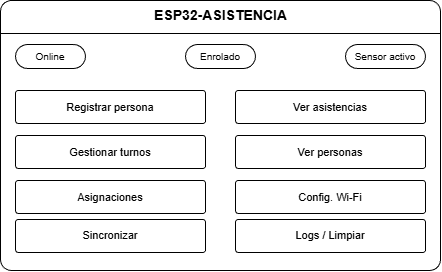
\includegraphics[width=.8\linewidth]{Imagenes/mockup_menu.png}
            \caption{Mockup menú principal en el ESP32-CAM.}
            \label{fig:mockup_menu}
        \end{figure}
        Wireframe inicial de la vista /: agrupa los indicadores de estado del dispositivo (conectividad, enrolamiento, sensor PIR) en la parte superior, y los accesos a cada módulo del sistema (registro, asistencias, turnos, personas, asignaciones, configuración Wi-Fi, sincronización y logs) como botones de navegación.

        \item Panel de configuración de Wi-Fi.
        \begin{figure}[H]
            \centering
            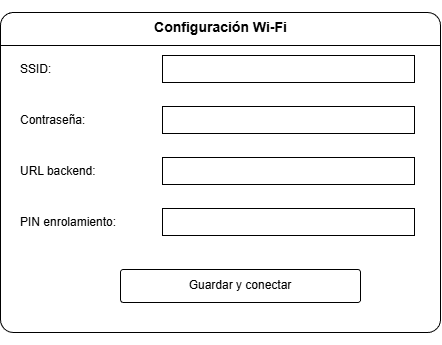
\includegraphics[width=.6\linewidth]{Imagenes/mockup_wifi.png}
            \caption{Mockup panel de configuración Wi-Fi.}
            \label{fig:mockup_wifi}
        \end{figure}
        Wireframe de la vista /wifi-setup: formulario con los cuatro campos que se persisten en wifi.json (SSID, contraseña de red, URL del backend y PIN de enrolamiento), accesible también desde el modo Access Point cuando el dispositivo no tiene credenciales configuradas.

        \item Vista de registro de usuario.
        \begin{figure}[H]
            \centering
            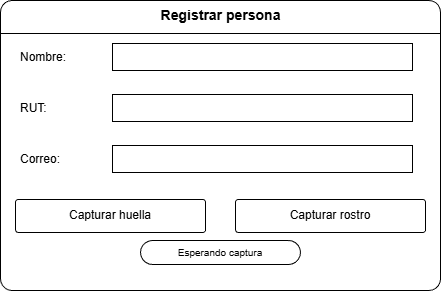
\includegraphics[width=.7\linewidth]{Imagenes/mockup_registro.png}
            \caption{Mockup registro de usuario en el ESP32-CAM.}
            \label{fig:mockup_registro}
        \end{figure}
        Wireframe de la vista /register: formulario de datos básicos (nombre, RUT, correo) seguido de los dos botones de captura biométrica, con un indicador de estado del proceso de enrolamiento (huella y rostro).

        \item Vista de usuarios almacenados localmente.
        \begin{figure}[H]
            \centering
            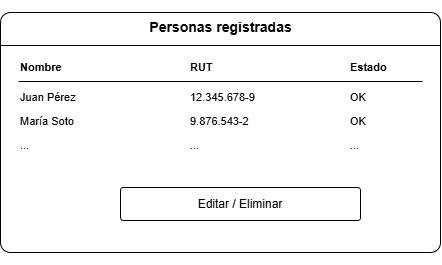
\includegraphics[width=.6\linewidth]{Imagenes/mockup_personas.png}
            \caption{Mockup de usuarios almacenados en el ESP32-CAM.}
            \label{fig:mockup_usuarios}
        \end{figure}
        Wireframe de la vista /personas: listado tabular de las personas registradas leídas desde personas.json, con acciones de edición y eliminación por fila.

        \item Vista de turnos almacenados localmente.
        \begin{figure}[H]
            \centering
            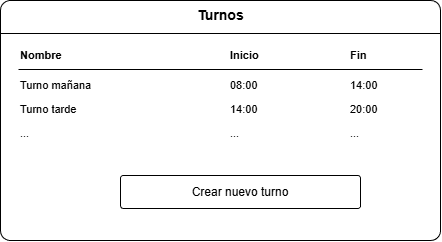
\includegraphics[width=.6\linewidth]{Imagenes/mockup_turnos.png}
            \caption{Mockup de visualización de turnos en el ESP32-CAM.}
            \label{fig:mockup_turnos}
        \end{figure}
        Wireframe de la vista /turnos: listado de los turnos almacenados en turnos.json, con el botón de acceso a la creación de un nuevo turno.

        \item Vista de crear turnos.
        \begin{figure}[H]
            \centering
            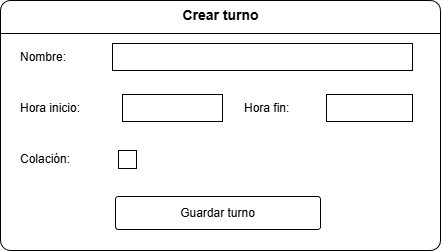
\includegraphics[width=.6\linewidth]{Imagenes/mockup_crear_turno.png}
            \caption{Mockup de creación de turnos en el ESP32-CAM.}
            \label{fig:mockup_crear_turnos}
        \end{figure}
        Wireframe de la vista /gestion: formulario para definir nombre, horario de inicio y fin, y la casilla opcional de colación que habilita los campos colacion\_inicio/colacion\_fin descritos en el Capítulo 4.

        \item Vista de asignación de turnos.
        \begin{figure}[H]
            \centering
            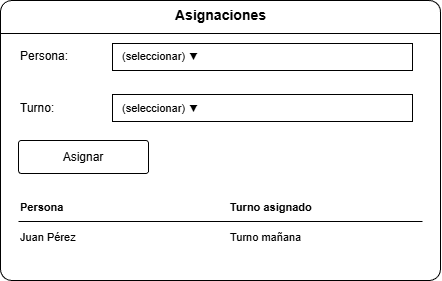
\includegraphics[width=.6\linewidth]{Imagenes/mockup_asignacion.png}
            \caption{Mockup de asignación de turnos en el ESP32-CAM.}
            \label{fig:mockup_asignacion}
        \end{figure}
        Wireframe de la vista /asignaciones: selección de persona y turno mediante listas desplegables, seguida del listado de asignaciones vigentes ya registradas.
    \end{itemize}

    \item \textbf{Diseño del flujo operacional}: a nivel conceptual, se planteó que el dispositivo debía capturar la huella o el rostro y luego evaluar si tenía conectividad disponible. Con conexión, la marcación se enviaría de inmediato al servidor; sin ella, se guardaría localmente para sincronizarse más adelante, cuando la red se restableciera. En ambos casos, la validación final (si la huella o el rostro corresponden a una persona registrada) ocurriría en el servidor, que respondería con un resultado de éxito o de error. El detalle de cómo se implementó cada uno de estos pasos, una vez que todos los componentes involucrados (enrolamiento, reconocimiento facial, sincronización diferida e integración ERP) estuvieron construidos, se presenta de forma consolidada al cierre del desarrollo, en la Sección~\ref{sec:flujo_operacional_consolidado}.
\end{itemize}

Estos elementos permiten visualizar el flujo básico del dispositivo antes de incorporar funcionalidades adicionales como turnos, sincronización o panel web backend, los cuales se desarrollarán en iteraciones posteriores.

\subsubsection{Implementación}

En esta etapa se integró tanto el hardware principal del prototipo como el desarrollo de las vistas web embebidas que permiten la interacción del usuario con el dispositivo. Para ello se utilizaron las siguientes librerías:

\begin{itemize}
    \item esp\_camera, utilizada para inicializar y configurar la cámara OV2640 integrada en el ESP32-CAM.
    \item HardwareSerial y Adafruit\_Fingerprint, empleadas para la comunicación UART con el lector biométrico AS608.
    \item WebServer, utilizada para montar un servidor web HTTP en el puerto 80 y atender rutas asociadas a las vistas.
    \item LittleFS y ArduinoJson \cite{arduinojson_docs}, empleadas para almacenamiento persistente en memoria flash y manipulación estructurada de datos JSON.
\end{itemize}

\paragraph{Integración del lector de huellas AS608}

El lector biométrico AS608 fue conectado directamente al ESP32-CAM mediante la interfaz UART secundaria (HardwareSerial 2), utilizando los pines GPIO14 (RX) y GPIO15 (TX). Esta conexión, que emplea pines distintos a los documentados inicialmente, fue forzada por la escasez de GPIO libres tras la asignación del bus de cámara. La velocidad de comunicación se estableció en 57600 baudios, y la librería Adafruit\_Fingerprint se vincula a dicho puerto serial. La Figura~\ref{fig:conexioneshuella} presenta la conexión física entre ambos dispositivos.

\begin{figure}[H]
    \centering
    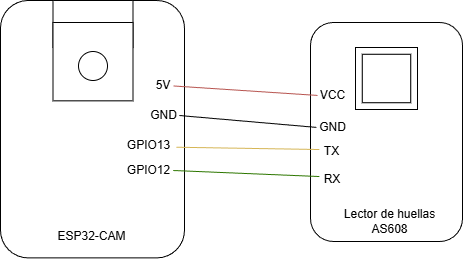
\includegraphics[width=.8\linewidth]{Imagenes/conexiones.png}
    \caption{Conexiones entre el ESP32-CAM y el lector de huellas AS608.}
    \label{fig:conexioneshuella}
\end{figure}

Una vez establecida la comunicación, el firmware puede ejecutar operaciones como:

\begin{itemize}
    \item Captura de imagen dactilar.
    \item Conversión de la imagen en una plantilla biométrica.
    \item Almacenamiento del template en un slot interno del sensor (1-127).
    \item Identificación mediante búsqueda de coincidencias en memoria.
\end{itemize}

La inicialización del lector se realiza con finger.begin(57600) sobre el puerto serie secundario, seguida de finger.verifyPassword() para confirmar que el sensor responde correctamente antes de habilitar las operaciones de captura, conversión y búsqueda descritas anteriormente.

\paragraph{Configuración de la cámara y el flash PWM}

La cámara OV2640 se configuró con resolución VGA (640×480) y compresión JPEG con calidad 8 (escala 0-63, donde valores bajos indican mayor calidad). La frecuencia del reloj externo (XCLK) se fijó en 20 MHz. Para evitar el parpadeo visible y las caídas de tensión provocadas por el flash LED durante la captura, se implementó un control PWM a 5 kHz con resolución de 8 bits, aplicando un ciclo de trabajo del 50\% (duty 128 de 255) durante la iluminación. Esto permite encender el flash con brillo suficiente sin sobrecargar la fuente de alimentación del ESP32-CAM.

\paragraph{Calibración del sensor PIR}

Se integró un sensor PIR (Passive Infrared) conectado al GPIO12 configurado con resistencia de pull-down interna. El sensor PIR actúa como detector de presencia: cuando una persona se sitúa frente al dispositivo, el PIR detecta el cambio de radiación infrarroja y activa el modo de captura. El setup incluye una fase de calibración de 3 segundos para estabilizar la lectura del sensor antes de iniciar el bucle principal. La lógica de uso del PIR como control de activación se detalla en la iteración 6.

\paragraph{Montaje del servidor web embebido}

Para habilitar la interacción local con el dispositivo, se implementó un servidor web mediante la librería WebServer en el puerto 80. Este servidor permite entregar páginas HTML, datos JSON y recursos estáticos. Cuando no hay conectividad a una red externa, el ESP32-CAM activa automáticamente un Access Point con SSID ESP32-ASISTENCIA y contraseña Asistencia2026, sirviendo las mismas páginas sin depender de internet.

Las rutas principales del sistema incluyen:

\begin{itemize}
    \item /: Menú principal con indicadores de estado.
    \item /wifi-setup: Configuración de red Wi-Fi y parámetros del backend.
    \item /register: Registro de personas con captura biométrica.
    \item /asistencias: Lista de asistencias almacenadas localmente.
    \item /gestion: Gestión de turnos (creación y administración).
    \item /personas: Visualización de personas registradas.
    \item /asignaciones: Vista para realizar asignaciones de turnos.
    \item /logs: Visualización de logs del sistema.
    \item /turnos: Visualización de turnos creados.
\end{itemize}

Para la implementación del servidor HTTP embebido, se utilizó el módulo WebServer del ESP32. Cada operación del sistema (registro de usuarios, captura de huellas, creación de turnos, asignación de turnos, lectura de asistencias, configuración Wi-Fi, entre otras) fue mapeada a un endpoint específico mediante funciones manejadoras (handler functions), registradas mediante "server.on(ruta, metodo, handler)" para cada una de las rutas listadas anteriormente. Este mecanismo permite encapsular la lógica de cada componente del sistema y mantener una estructura modular del firmware.

\paragraph{Creación de vistas HTML embebidas}

Las vistas fueron desarrolladas como archivos .html independientes almacenados en el sistema de archivos LittleFS del ESP32-CAM, conteniendo HTML, CSS y JavaScript autónomo, sin dependencias de CDN externas. El servidor web embebido las sirve mediante la función servirArchivo(), que lee el archivo solicitado desde LittleFS y lo envía al cliente. Esto garantiza que el ESP32-CAM sirva cada página incluso en modo Access Point sin conexión a internet.

\paragraph{Menú principal}

La Figura~\ref{fig:menu_principal} presenta la vista principal accesible en la ruta /. Desde esta interfaz el usuario puede visualizar el estado del dispositivo (online/offline, sensor activo, enrolado), registrar personas, ver asistencias, gestionar turnos, ver asignaciones, acceder a la configuración de red, sincronizar con el backend y limpiar datos del dispositivo. Con el avance de las iteraciones se agregaron a esta vista los indicadores de estado que se actualizan cada pocos segundos consultando al dispositivo, un bloque para mostrar el PIN de registro que permanece oculto hasta que el usuario decide revelarlo, una zona separada para las acciones de reinicio y borrado total de datos, y la opción de proteger la página con contraseña de administrador cuando se requiere restringir el acceso a esas acciones.

\begin{figure}[H]
    \centering
    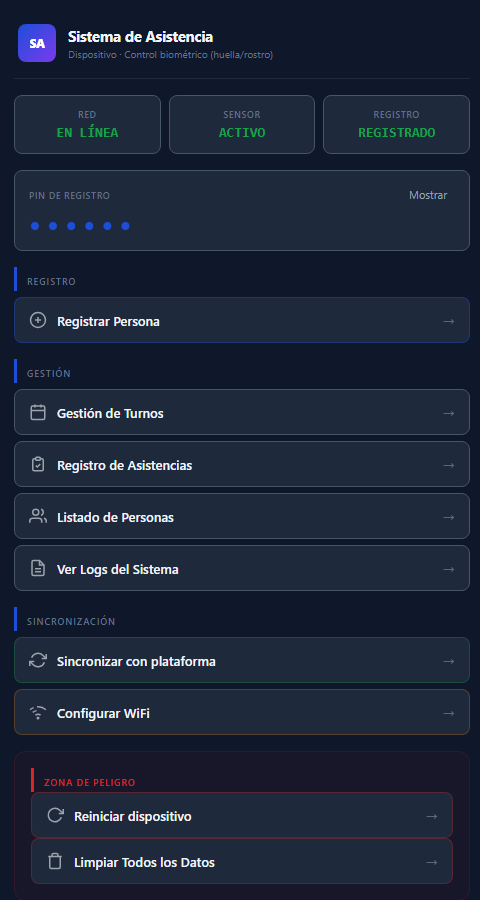
\includegraphics[height=8.5cm,keepaspectratio]{Imagenes/menuimplementado.png}
    \caption{Menú principal del sistema web embebido.}
\label{fig:menu_principal}
\end{figure}

\paragraph{Vista de configuración Wi-Fi}

Mediante la ruta /wifi-setup, el dispositivo proporciona un formulario para actualizar las credenciales de la red local (SSID, contraseña), la URL del backend, la dirección del broker MQTT y el PIN de enrolamiento. Estos valores se persisten en SPIFFS mediante el archivo wifi.json. La Figura~\ref{fig:wifi_config} muestra esta interfaz. Por requerimientos de seguridad identificados en iteraciones posteriores, se agregó a esta vista la opción de forzar conexiones cifradas hacia el backend y el broker MQTT, además de un apartado donde se puede definir o cambiar la contraseña de administrador pidiendo la contraseña actual como confirmación, de modo que no cualquier persona con acceso a la red local pueda modificar la configuración del dispositivo.

\begin{figure}[H]
    \centering
    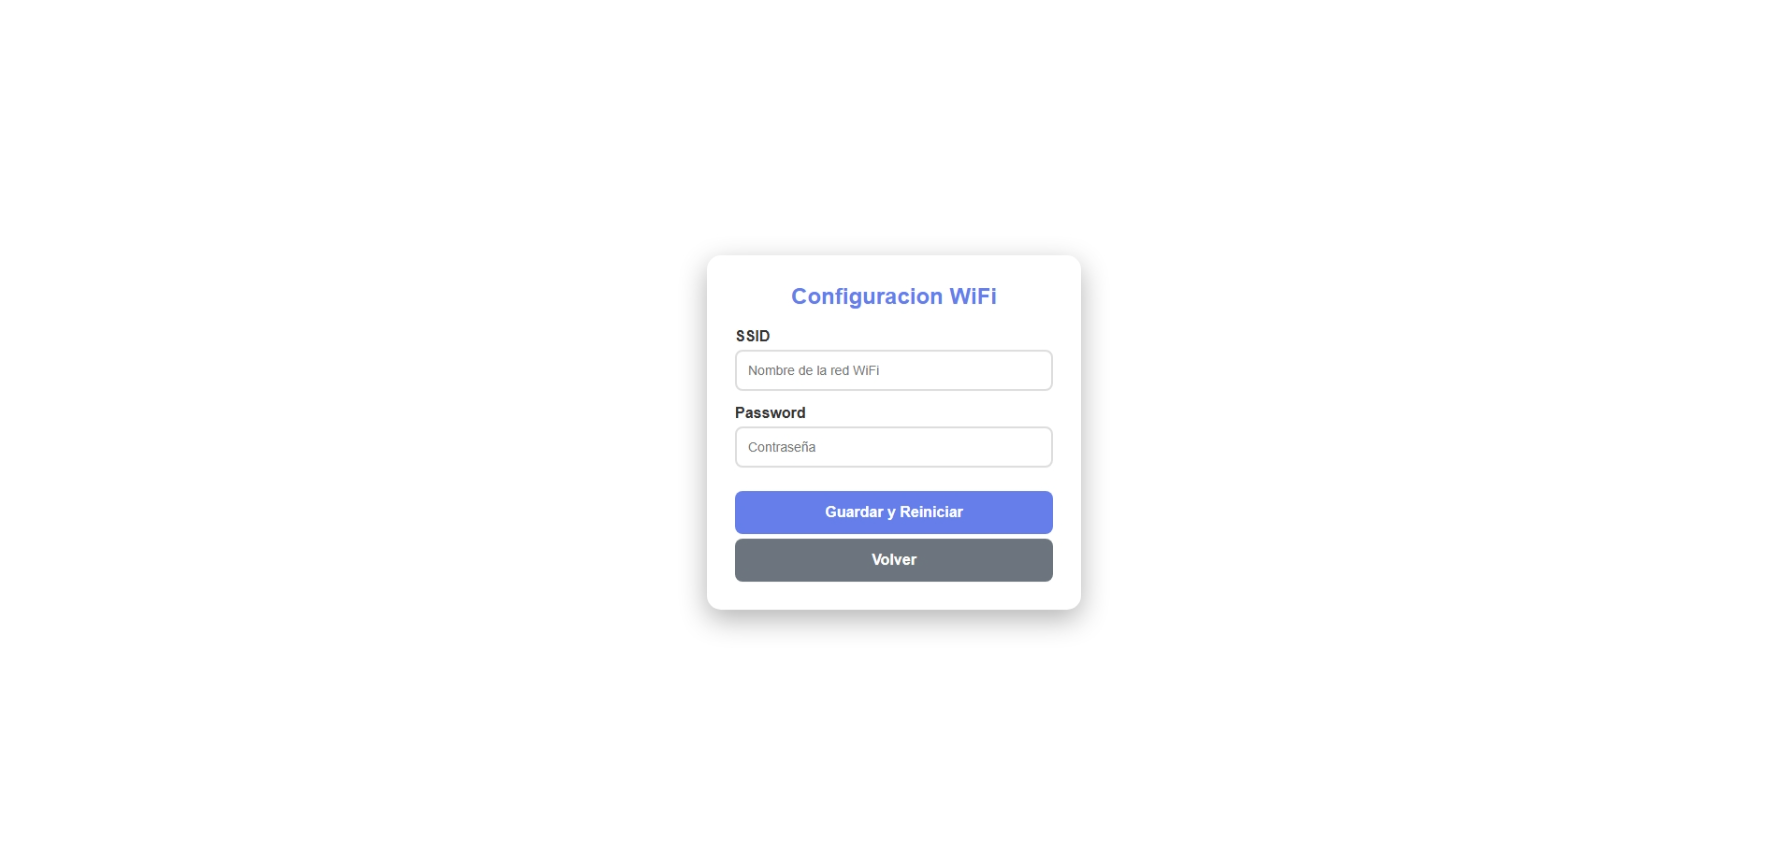
\includegraphics[height=8.5cm,keepaspectratio]{Imagenes/menuwifiimplementado.png}
    \caption{Interfaz de configuración Wi-Fi.}
\label{fig:wifi_config}
\end{figure}

\paragraph{Vista de registro de personas}

La ruta /register despliega una vista que combina un formulario para ingresar el nombre del usuario, RUT y correo electrónico, y muestra indicadores visuales del estado del proceso de enrolamiento (huella, rostro). La Figura~\ref{fig:registro_personas} lo muestra. Se incorporó a esta vista una casilla de consentimiento explícito para el tratamiento de datos biométricos, exigida por las consideraciones éticas y de privacidad descritas en el marco metodológico; mientras no se marque, el botón para iniciar el registro biométrico queda deshabilitado. El flujo se complementó además con un panel que informa el avance del proceso y con una pantalla de captura facial guiada, que muestra cuántas de las tres fotografías necesarias para el reconocimiento facial ya se han tomado.

\begin{figure}[H]
    \centering
    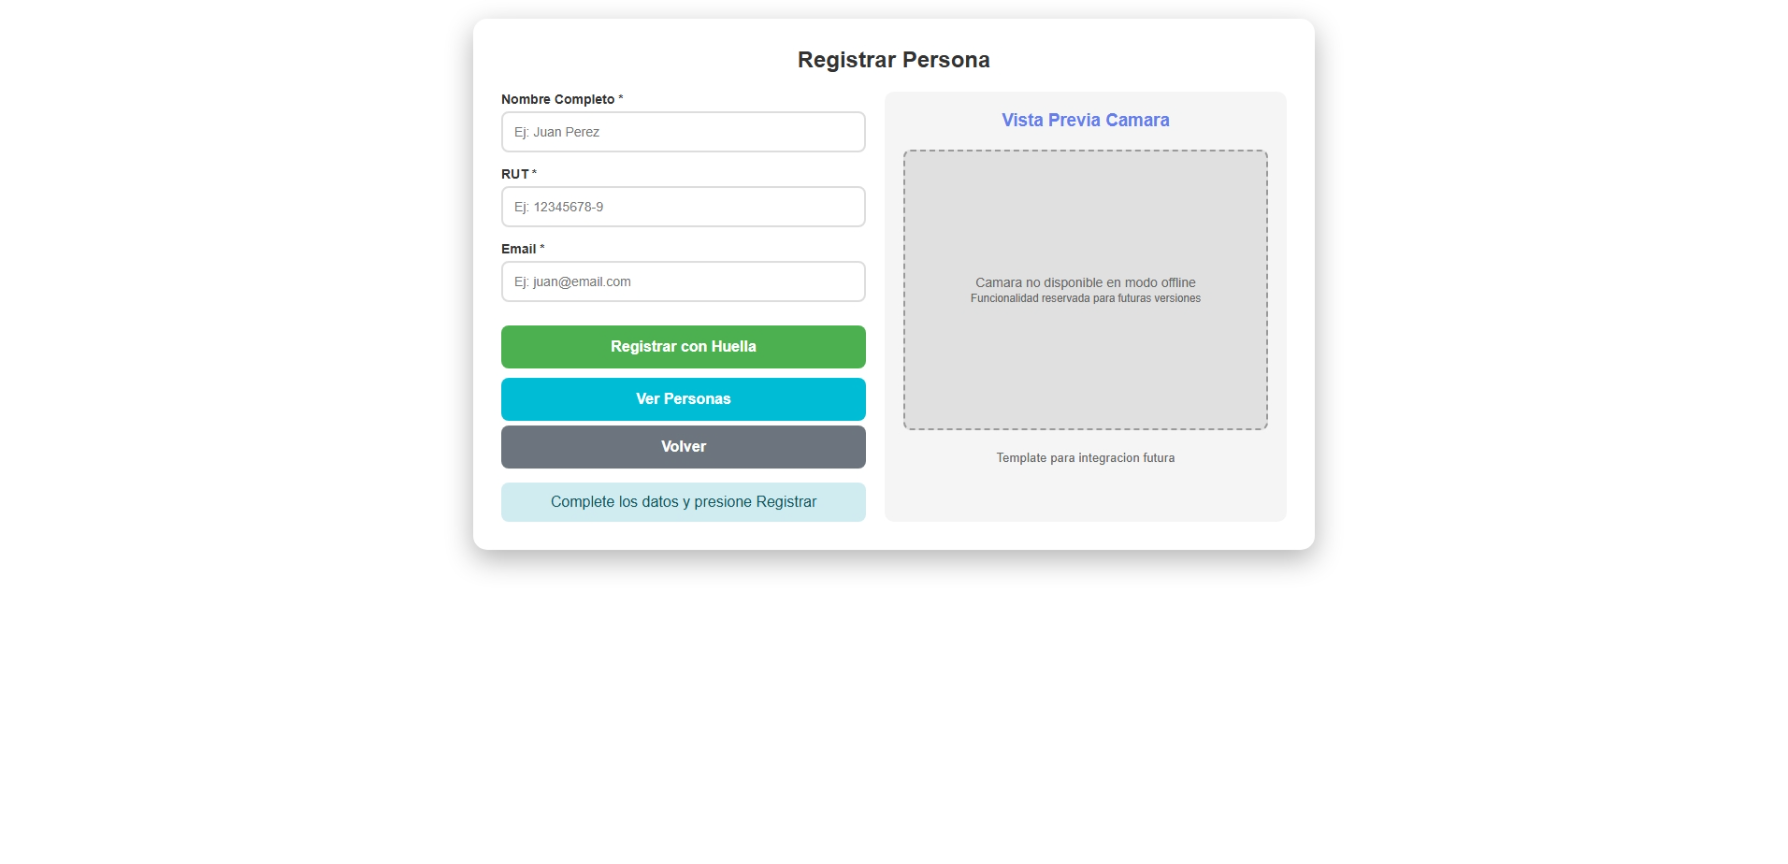
\includegraphics[height=8.5cm,keepaspectratio]{Imagenes/registroimplementado.png}
    \caption{Vista para el registro de personas en el dispositivo.}
\label{fig:registro_personas}
\end{figure}

\paragraph{Vista de asistencias}

Para visualizar registros de asistencia tanto locales como sincronizados, se implementó la vista en la ruta /asistencias. Esta consulta archivos JSON almacenados en LittleFS. La Figura~\ref{fig:vista_asistencias} lo ejemplifica. Cada registro se presenta como una tarjeta diferenciada por color según sea entrada o salida, con el nombre de la persona, la marca de tiempo y su identificador asociado. A la versión inicial, que solo listaba los registros, se le agregaron las opciones de editar o eliminar cada fila, pensadas para que el encargado de turno pueda corregir una marcación errónea, como una doble lectura biométrica, sin necesidad de acceder directamente al backend. También se sumó un contador de registros totales en la parte superior, útil para revisar de un vistazo cuántos datos hay almacenados localmente antes de sincronizar.

\begin{figure}[H]
    \centering
    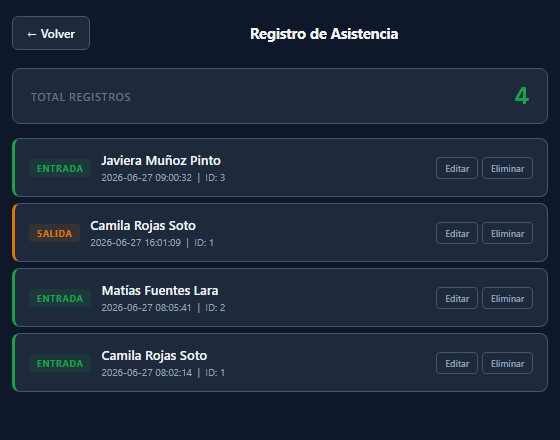
\includegraphics[height=8.5cm,keepaspectratio]{Imagenes/vistaasitenciasimplementado.png}
    \caption{Vista de asistencias locales almacenadas en el dispositivo.}
\label{fig:vista_asistencias}
\end{figure}

\paragraph{Vista de Personas registradas}

Para visualizar las personas registradas, se implementó la vista en la ruta /personas. Esta consulta archivos JSON almacenados en LittleFS y permite editar nombre/correo, actualizar huella o rostro, y eliminar personas. La Figura~\ref{fig:personas_registradas} lo ejemplifica. Las opciones para actualizar la huella o el rostro, y para agregar fotos adicionales, se incorporaron después de notar en las pruebas de campo que volver a registrar a una persona desde cero, borrando y repitiendo todo el proceso, tomaba demasiado tiempo. Con estas opciones se puede corregir solo la huella o el rostro de alguien ya registrado, o sumar fotos para mejorar el reconocimiento facial, sin perder el resto de sus datos ni su historial de asistencia.

\begin{figure}[H]
    \centering
    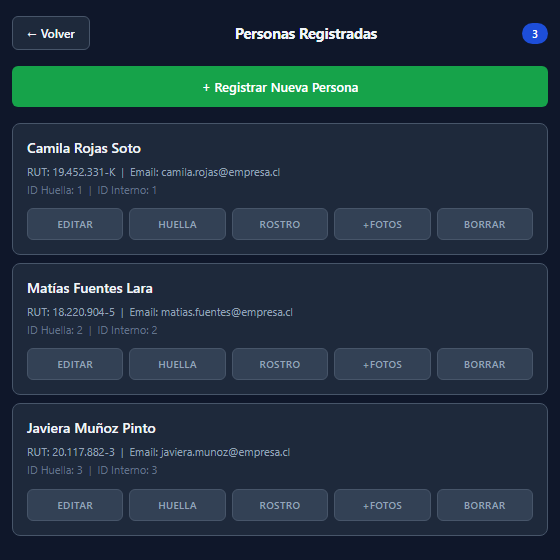
\includegraphics[height=8.5cm,keepaspectratio]{Imagenes/personasregistradasimplementada.png}
    \caption{Vista de personas registradas en el dispositivo.}
\label{fig:personas_registradas}
\end{figure}

\paragraph{Vista de Crear Turnos}

Para la creación de turnos y visualización de los existentes, se implementó la vista en la ruta /gestion, complementada con /turnos. Estas consultan archivos JSON almacenados en LittleFS. La Figura~\ref{fig:gestion_turnos} lo ejemplifica. La vista /gestion funciona como panel resumen, con accesos directos a la gestión de turnos, a las asignaciones y a la sincronización manual con la plataforma. La vista /turnos concentra el formulario para crear un turno nuevo, con nombre, hora de inicio y fin, y un selector de días de la semana, junto con el listado editable de los turnos ya creados. Esta separación entre resumen y edición se introdujo para que las modificaciones no ocurran por accidente desde la pantalla que se usa con más frecuencia.

\begin{figure}[H]
    \centering
    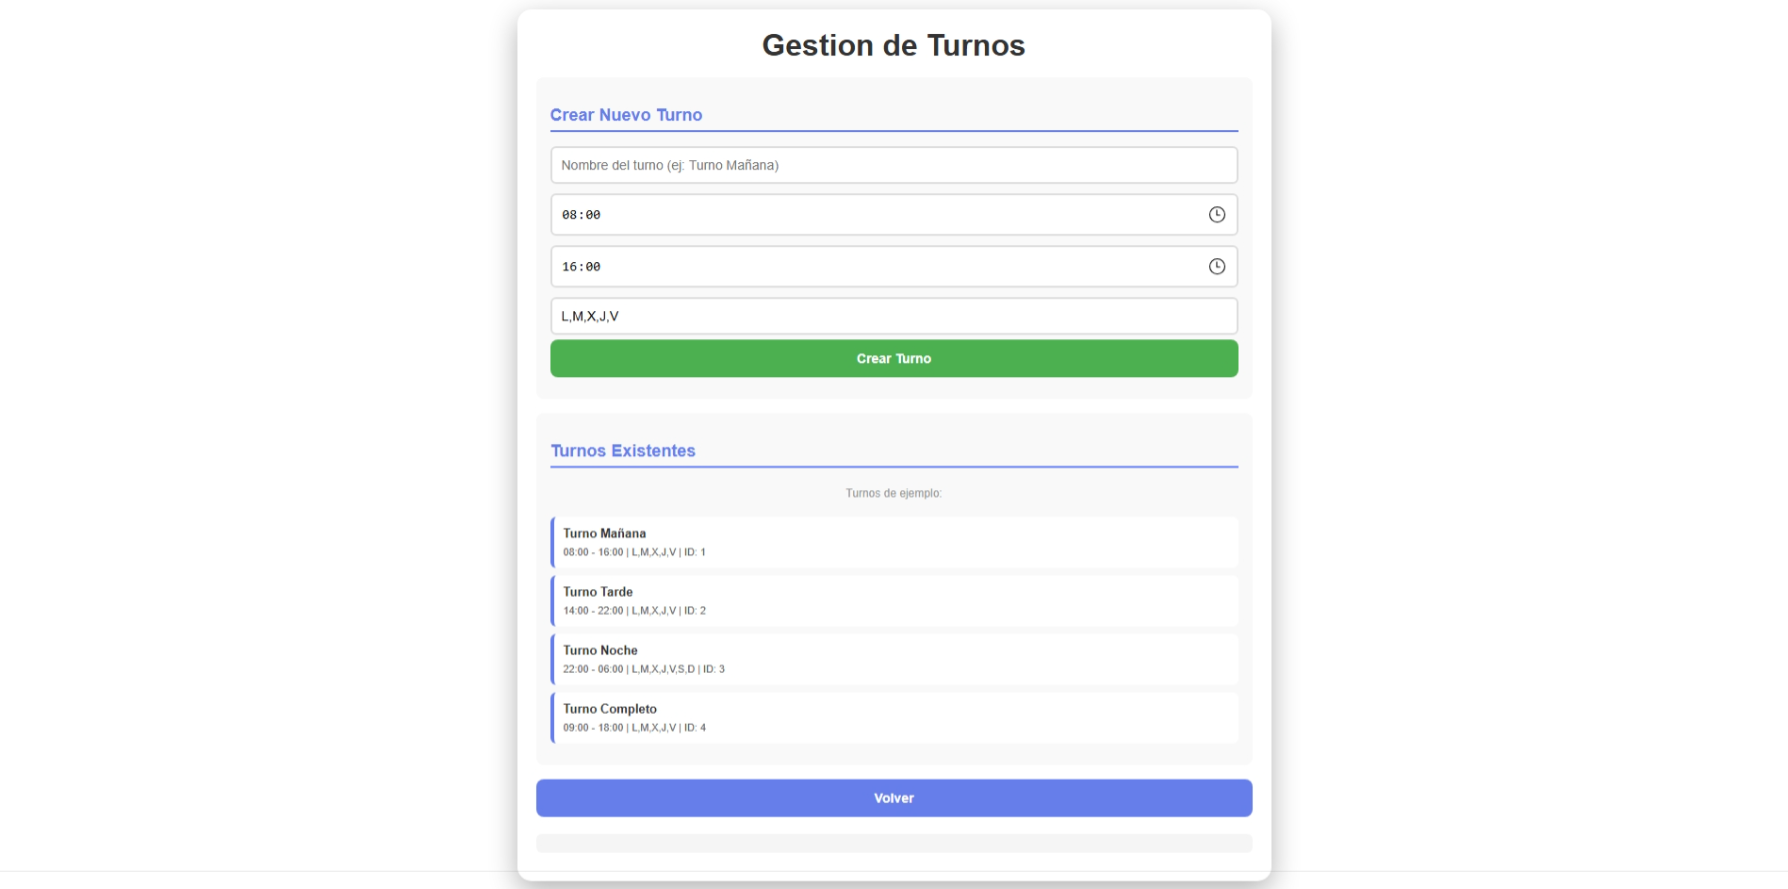
\includegraphics[height=8.5cm,keepaspectratio]{Imagenes/creacionturnos.png}
    \caption{Vista de gestión y creación de turnos en el dispositivo.}
\label{fig:gestion_turnos}
\end{figure}

\paragraph{Vista de asignación de turnos}

Para visualizar las asignaciones de turnos y realizar la acción de asignar un turno a una persona, se implementó la vista en la ruta /asignaciones. La Figura~\ref{fig:asignacion_turnos} lo ejemplifica. El formulario superior permite elegir una persona y un turno ya creados desde listas desplegables, evitando que el usuario tenga que recordar o escribir identificadores internos. El listado de asignaciones actuales muestra el nombre de la persona y del turno en lugar de solo sus identificadores, e incluye una opción para quitar una asignación, agregada después de notar que reasignar turnos por cambios de horario del personal era algo que ocurría seguido durante el uso del prototipo.

\begin{figure}[H]
    \centering
    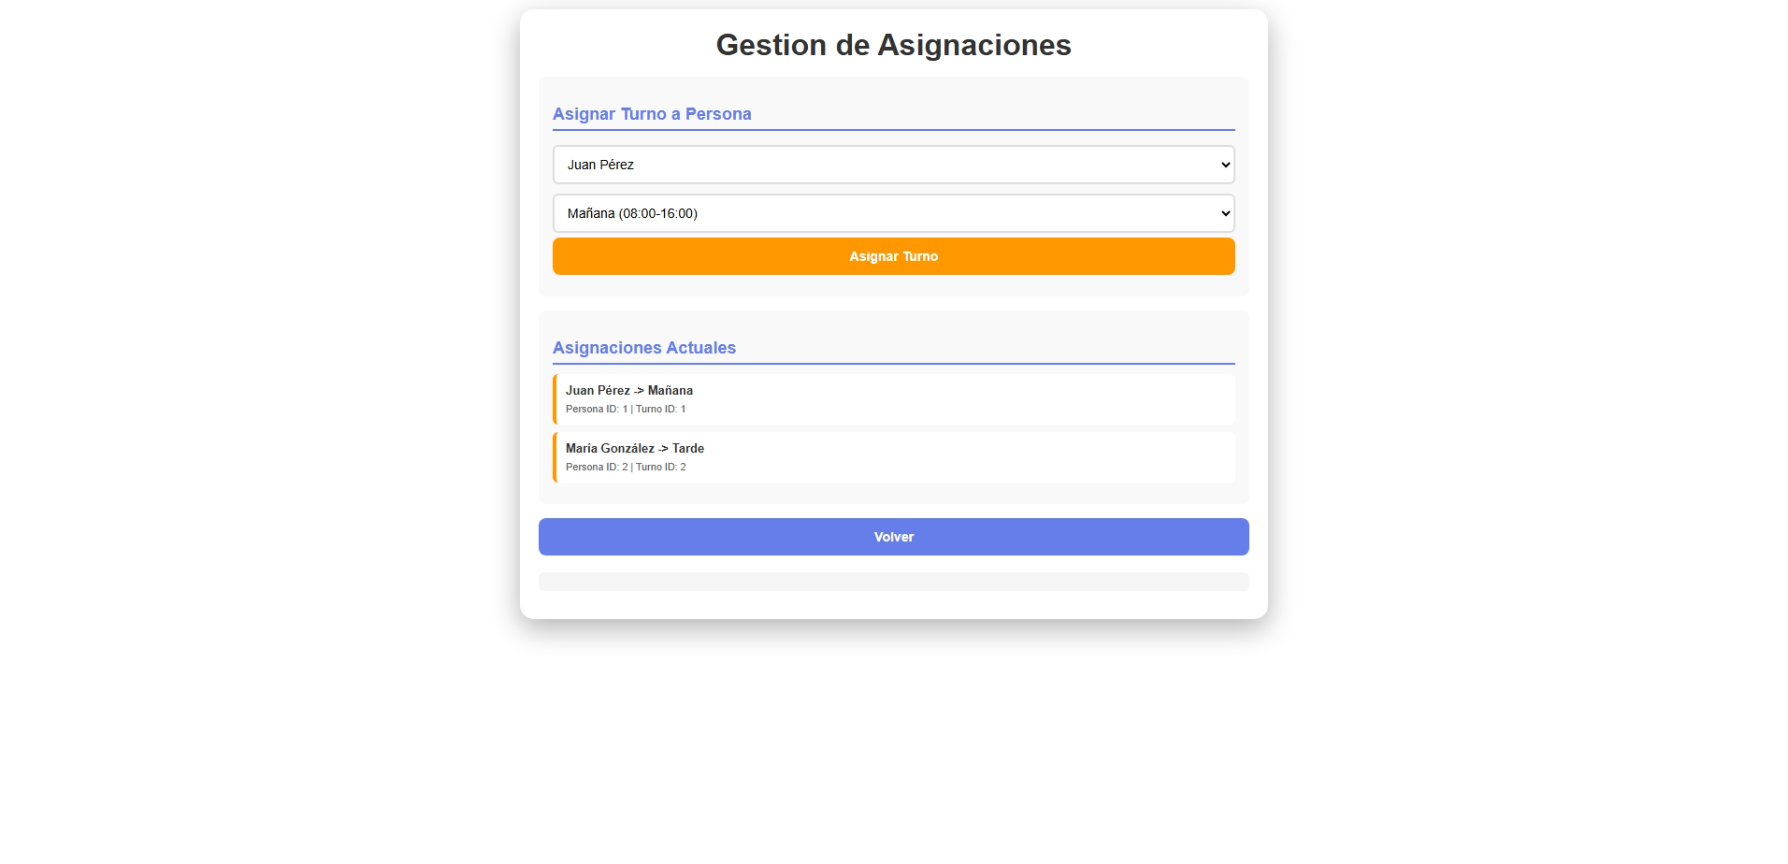
\includegraphics[height=8.5cm,keepaspectratio]{Imagenes/asignacionturnoimplementacion.png}
    \caption{Vista de gestión de asignaciones en el dispositivo.}
\label{fig:asignacion_turnos}
\end{figure}

\subsubsection{Pruebas}

Para validar el funcionamiento del prototipo y comprobar la correcta integración entre los distintos módulos del sistema, se diseñaron pruebas de integración enfocadas exclusivamente en los componentes implementados durante esta iteración:

\begin{itemize}
    \item \textbf{Prueba de captura de imágenes}: Verificar que la cámara OV2640 capture imágenes JPEG de forma continua y estable, sin corrupción de frames ni errores de inicialización del sensor. Se espera que la función esp\_camera\_fb\_get() retorne buffers consistentes tras cada llamada.

    \item \textbf{Prueba de comunicación UART con AS608}: Verificar que el lector biométrico responda correctamente al comando de verificación de contraseña (finger.verifyPassword()) y que la comunicación serie a 57600 baudios se establezca sin pérdida de paquetes. Se espera confirmación de conexión en menos de 1 segundo tras el inicio.

    \item \textbf{Prueba de lectura biométrica}: Verificar que el AS608 pueda capturar una imagen dactilar (finger.getImage()), convertirla a plantilla (finger.image2Tz()) y almacenarla en un slot del sensor (finger.storeModel()). Se espera que el proceso completo tome menos de 2 segundos.

    \item \textbf{Prueba de acceso vía AP}: Verificar que al iniciar sin credenciales Wi-Fi configuradas, el ESP32-CAM active el Access Point ESP32-ASISTENCIA y que las páginas HTML sean accesibles desde un navegador conectado a la IP 192.168.4.1. Se espera que todas las rutas definidas respondan con código HTTP 200.

    \item \textbf{Prueba de carga de vistas vía Wi-Fi externa}: Verificar que al conectar el dispositivo a una red Wi-Fi configurada, las mismas vistas se carguen correctamente a través de la IP asignada por el router, manteniendo estilos, scripts y funcionalidad.
\end{itemize}

\subsubsection{Refinamientos posteriores}

Durante el desarrollo de las iteraciones siguientes surgieron dos problemas asociados a la base construida en esta etapa, los cuales fueron corregidos durante el mismo ciclo de implementación.

El primero se presentó al combinar las funcionalidades de conectividad y enrolamiento: un dispositivo podía encontrarse conectado a internet sin contar aún con una persona enrolada, o bien tener una persona enrolada pero haber perdido la conexión de red. En ambos casos, el firmware intentaba ejecutar la sincronización o el reconocimiento facial de igual forma, lo que provocaba fallos sin generar un mensaje de error claro para el usuario. Para resolver esta situación, se implementó una función de validación que verifica simultáneamente ambas condiciones antes de permitir cualquier operación dependiente del backend, evitando así que el dispositivo ejecute procesos que se sabe resultarán en error.

El segundo ajuste estuvo relacionado con la calidad de las imágenes utilizadas para el reconocimiento facial. Las capturas estándar de la cámara se almacenaban con un nivel de compresión orientado a vistas previas rápidas, el cual resultaba insuficiente para generar un embedding facial de calidad adecuada, debido a la pérdida de detalle en los rasgos del rostro. Por este motivo, se diferenció el proceso de captura correspondiente al registro biométrico, incrementando temporalmente la resolución del sensor exclusivamente para la fotografía de referencia, y restableciéndola a su configuración estándar una vez completada la captura, sin afectar el resto de las imágenes procesadas por el sistema.

%% ============================================================
%% ITERACIÓN 2: Almacenamiento local y modo offline
%% ============================================================

\subsection{Iteración 2: Almacenamiento local y modo offline}

La segunda iteración se centra en habilitar el funcionamiento autónomo del dispositivo sin conexión a internet, integrando un sistema de almacenamiento persistente basado en LittleFS (sucesor moderno de SPIFFS para ESP32) y los mecanismos de captura biométrica offline. Esta etapa materializa lo definido en el apartado 3.1.2 del capítulo anterior.

\subsubsection{Análisis}

Para el correcto funcionamiento offline del prototipo se identificaron los siguientes requerimientos:

\begin{itemize}
    \item Almacenar localmente los datos de usuarios, turnos, asignaciones y asistencias en formato JSON.
    \item Permitir el registro de marcaciones aun cuando no exista conectividad externa, tanto por huella (offline total) como con validación de turnos locales.
    \item Garantizar persistencia de la información tras reinicios del ESP32-CAM o cortes de energía.
    \item Habilitar la gestión completa del sistema mediante una interfaz web embebida accesible vía Access Point.
    \item Mantener compatibilidad con la futura sincronización automática en modo online, marcando cada registro con un campo sincronizado (booleano) para su posterior envío al backend.
\end{itemize}

Para cumplir estos requisitos se seleccionó el sistema de archivos LittleFS y el formato JSON debido a su bajo peso, facilidad de manipulación mediante la librería ArduinoJson y compatibilidad con las capacidades del ESP32-CAM (4 MB de flash, de los cuales aproximadamente 1.5 MB están disponibles para LittleFS). Adicionalmente, se definió un archivo de configuración, wifi.json, destinado a almacenar credenciales Wi-Fi, URL del backend, dirección del broker MQTT y PIN de enrolamiento.

\subsubsection{Diseño}

Considerando la arquitectura establecida, se diseñaron las siguientes estructuras de almacenamiento en formato JSON:

\begin{itemize}
    \item \textbf{personas.json}: Arreglo de objetos con campos id, nombre, rut, email, huella\_id, fecha\_registro, sincronizado.
    \item \textbf{turnos.json}: Arreglo de objetos con campos id, backend\_id, nombre, inicio, fin, dias, sincronizado.
    \item \textbf{asignaciones.json}: Arreglo de objetos con campos persona\_id, turno\_id, backend\_id, fecha\_asignacion, sincronizado.
    \item \textbf{asistencias.json}: Arreglo de objetos con campos persona\_id, nombre, tipo (entrada/salida), metodo (huella\_offline, facial, etc.), timestamp, sincronizado.
    \item \textbf{wifi.json}: Objeto con campos ssid, pass, backend, mqtt, pin (para enrolamiento del dispositivo).
    \item \textbf{erp-config.json}: Arreglo con configuraciones de integraciones ERP, sincronizado desde el backend cuando hay conectividad.
\end{itemize}

El campo sincronizado (booleano) en cada entidad actúa como bandera para el proceso de sincronización diferida: cuando el dispositivo recupera conectividad, itera sobre los registros con sincronizado = false y los envía al backend. Una vez confirmada la recepción, se marca sincronizado = true.

\subsubsection{Implementación}

En esta iteración se integraron las librerías LittleFS, ArduinoJson, HardwareSerial y Adafruit\_Fingerprint. Las dos primeras permiten gestionar archivos JSON alojados en la memoria flash del ESP32-CAM, mientras que las dos últimas habilitan la comunicación UART con el lector biométrico AS608 para el registro y verificación de huellas digitales.

\paragraph{Inicialización del sistema de archivos y persistencia}

El primer componente de la implementación consiste en montar LittleFS mediante LittleFS.begin(true) y verificar la existencia de los archivos necesarios. En caso de no existir, el sistema los crea con una estructura inicial vacía (arreglo [] para las colecciones, objeto con valores por defecto para wifi.json), asegurando que el dispositivo pueda operar incluso tras un primer arranque sin configuración previa.

Se implementaron dos funciones genéricas para la manipulación de archivos JSON:

\begin{itemize}
    \item loadArray(const char* path, DynamicJsonDocument\& doc): Abre un archivo, deserializa su contenido como JsonArray y lo retorna. Si el archivo no existe o está corrupto, retorna un arreglo vacío.
    \item saveArray(const char* path, DynamicJsonDocument\& doc): Serializa el documento JSON y lo escribe en el archivo correspondiente, sobrescribiendo el contenido anterior.
\end{itemize}

Estas funciones encapsulan toda la lógica de persistencia del sistema y son reutilizadas por todos los módulos que necesiten leer o escribir datos.

El tamaño de cada DynamicJsonDocument se dimensionó según el volumen esperado de datos de cada archivo, aunque varía según la función que lo utiliza: asignaciones.json utiliza típicamente 1024~bytes, personas.json y turnos.json se manejan con buffers de entre 2048 y 8192~bytes dependiendo del contexto (lectura local, sincronización o registro), y asistencias.json utiliza 32768~bytes. Adicionalmente, en la función procesarAsistencia() se incorporó una validación sobre el retorno de createNestedObject(): si el objeto retornado es nulo (indicando desbordamiento del documento), se registra una advertencia en el log del sistema, permitiendo detectar tempranamente cuellos de botella de memoria sin comprometer la integridad del archivo JSON. El dimensionamiento de este buffer y la estrategia adoptada para sostener el volumen de registros exigido en los objetivos del proyecto se detallan en el apartado de refinamientos posteriores de esta iteración.

\paragraph{Registro de usuarios con huella digital}

El registro de usuarios se implementó mediante un flujo que combina la captura biométrica gestionada por el lector AS608 con el almacenamiento en personas.json. El lector administra internamente modelos de huellas mediante \textit{slots} numerados del 1 al 127. Por ello, antes del enrolamiento es necesario identificar un slot disponible dentro del sensor. La función encontrarSlotLibre() recorre el arreglo de personas, determina el ID de huella más alto registrado y retorna el siguiente disponible.

Una vez encontrado un slot, se ejecuta el proceso de enrolamiento en dos fases:

\begin{enumerate}
    \item \textbf{Primera captura} (ESTADO\_ESPERANDO\_HUELLA\_REGISTRO): El sistema espera que el usuario coloque el dedo. Al detectar una imagen válida, la convierte a plantilla en el buffer 1 y transiciona a ESTADO\_ESPERANDO\_SOLTAR\_DEDO.
    \item \textbf{Espera y segunda captura} (ESTADO\_REGISTRO\_SEGUNDA\_HUELLA): Una vez que el sensor detecta que el dedo fue retirado (FINGERPRINT\_NOFINGER), el sistema solicita una segunda captura del mismo dedo. Al obtenerla, convierte a plantilla en el buffer 2, crea el modelo combinado (finger.createModel()) y lo almacena en el slot correspondiente (finger.storeModel()).
\end{enumerate}

Luego del enrolamiento exitoso, se almacena un nuevo objeto dentro de personas.json con un identificador único (generado localmente con prefijo local- o provisto por el backend si hay conectividad), el nombre, RUT, correo electrónico y el slot asignado. La etapa de captura de huella aquí descrita corresponde a los primeros estados de la máquina de estados del registro biométrico completo, presentada más adelante en la Figura~\ref{fig:maquina_estados_esp32} (sección 4.3.4), una vez introducido el envío de la foto de referencia al backend por HTTP.

\paragraph{Registro de asistencia en modo offline}

El registro de asistencia se realiza completamente en el dispositivo, sin necesidad de conexión externa. El flujo implementado consiste en:

\begin{enumerate}
    \item Capturar una huella mediante el lector AS608 (finger.getImage()).
    \item Convertir la imagen a plantilla (finger.image2Tz()) y ejecutar una búsqueda biométrica (finger.fingerSearch()) que retorna el fingerID del slot coincidente.
    \item Identificar al usuario asociado mediante el campo huella\_id en personas.json con la función buscarPersonaPorHuella().
    \item Verificar que el usuario cuente con un turno asignado consultando asignaciones.json mediante turnoActivo(). Si no tiene turno, el sistema rechaza la marcación.
    \item Determinar el tipo de evento (entrada/salida) alternando automáticamente respecto al último registro de la persona en asistencias.json.
    \item Generar un nuevo registro con sincronizado = false (salvo que se logre enviar al backend en ese momento).
\end{enumerate}

El manejador handleMarcarAsistencia() expone esta funcionalidad a través de la interfaz web, permitiendo también marcaciones manuales. El escaneo automático continuo se controla mediante intervalos configurables: 2 segundos entre verificaciones de huella y 6 segundos entre verificaciones faciales.

\paragraph{Gestión de turnos y asignaciones}

Además del registro de asistencias, el sistema permite crear turnos (handleCreateTurn()) y asignarlos a personas (handleAssignTurn()) desde la interfaz web. Cada operación persiste los datos en sus archivos JSON correspondientes y, si hay conectividad, intenta replicar la operación en el backend mediante HTTP POST.

\paragraph{Operación offline del dispositivo}

Con el objetivo de asegurar autonomía total, el ESP32-CAM fue configurado para operar en dos modos:

\begin{itemize}
    \item \textbf{Modo Wi-Fi STA}: Si hay credenciales configuradas en wifi.json, el dispositivo intenta conectarse a la red externa. Si la conexión falla reiteradamente (5 intentos), activa el modo AP como fallback sin deshabilitar el intento de reconexión.
    \item \textbf{Modo Access Point}: El punto de acceso utiliza el SSID ESP32-ASISTENCIA y contraseña Asistencia2026, permitiendo que un administrador se conecte directamente al dispositivo en la IP 192.168.4.1 para realizar todas las operaciones mediante la interfaz web embebida.
\end{itemize}

\subsubsection{Pruebas}

Se diseñaron las siguientes pruebas para validar el correcto funcionamiento del almacenamiento local y el modo offline:

\begin{itemize}
    \item \textbf{Prueba de persistencia tras reinicio}: Registrar usuarios, turnos, asignaciones y asistencias, luego reiniciar el ESP32-CAM (por corte de energía o comando software). Verificar que todos los archivos JSON conserven su contenido íntegro y que el sistema pueda leerlos correctamente tras el reinicio.

    \item \textbf{Prueba de lectura y deserialización}: Abrir cada archivo JSON generado y verificar que ArduinoJson pueda deserializar su contenido sin errores ni pérdida de campos. El tamaño de cada DynamicJsonDocument se configuró según la capacidad esperada del archivo: 2048~bytes para personas.json y turnos.json, 1024~bytes para asignaciones.json y 32768~bytes para asistencias.json. Se incluyó además una validación post-inserción (mediante isNull()) en la función procesarAsistencia() para detectar y registrar en logs cualquier desbordamiento del documento al crear nuevos registros de asistencia.

    \item \textbf{Prueba de escritura concurrente}: Realizar múltiples operaciones de escritura (registro de persona + asignación de turno + marcación de asistencia) en rápida sucesión sin reiniciar el sistema. Verificar que no se produzcan corrupciones de archivos ni pérdida de datos.

    \item \textbf{Prueba de marcación offline por huella}: Desconectar el dispositivo de toda red externa, registrar un usuario con huella y turno, y efectuar una marcación. Verificar que el registro aparezca en asistencias.json con sincronizado = false.

    \item \textbf{Prueba de alternancia entrada/salida}: Realizar dos marcaciones consecutivas para un mismo usuario. Verificar que el sistema registre correctamente ``entrada'' seguido de ``salida''.

    \item \textbf{Prueba de validación de turno offline}: Intentar marcar asistencia para un usuario sin turno asignado. Verificar que el sistema rechace la marcación con el mensaje ``Sin turno asignado''.

    \item \textbf{Prueba de funcionamiento del AP}: Desconectar el ESP32-CAM de cualquier red, verificar que el AP ESP32-ASISTENCIA se active automáticamente y que todas las operaciones de gestión (registro, turnos, asignaciones, asistencias) funcionen correctamente desde un navegador conectado a la IP 192.168.4.1.
\end{itemize}

\subsubsection{Refinamientos posteriores}

Durante la revisión de esta iteración se identificó una limitación que comprometía directamente el objetivo específico de sostener al menos 1.000 registros de asistencia almacenados de forma segura en LittleFS. El diseño original cargaba el archivo asistencias.json completo en un único DynamicJsonDocument cada vez que se necesitaba leer o escribir un registro, de modo que la capacidad práctica del sistema no estaba acotada por el espacio disponible en la memoria flash —de varios megabytes y suficiente para almacenar miles de registros en formato JSON— sino por el tamaño del buffer reservado en RAM. Con el buffer original de 8192~bytes la capacidad estimada era de apenas unas decenas de registros, muy por debajo de lo exigido en los objetivos del proyecto.

Adicionalmente, se observó que los registros ya sincronizados con el backend no se eliminaban del archivo local: la función sincronizarAsistencias() únicamente actualizaba el campo sincronizado a true, por lo que el arreglo en memoria crecía de forma indefinida durante toda la vida útil del dispositivo, incluso operando con conectividad constante.

Para corregir esta situación se aplicaron dos ajustes complementarios. Primero, se incrementó el tamaño del DynamicJsonDocument utilizado para asistencias.json de 8192 a 32768~bytes, ampliando el margen disponible para los registros pendientes de sincronización. Segundo, y de mayor relevancia, se modificó sincronizarAsistencias() para que, una vez confirmada la recepción exitosa por parte del backend, los registros marcados como sincronizados sean eliminados del archivo local en lugar de conservarse indefinidamente. De esta forma, el buffer en RAM solo necesita reservar espacio para los registros generados durante un período sin conectividad, mientras que el historial completo de marcaciones queda respaldado de manera permanente en el backend. Esta estrategia permite que el dispositivo sostenga miles de marcaciones acumuladas a lo largo de su operación sin acercarse al límite de memoria, cumpliendo así el volumen exigido por el objetivo específico correspondiente, condicionado a que el dispositivo sincronice periódicamente con el backend.

%% ============================================================
%% ITERACIÓN 3: Backend, base de datos, HTTP y MQTT
%% ============================================================

\subsection{Iteración 3: Backend, base de datos y comunicación}

El propósito de esta iteración consiste en implementar un backend centralizado que permita procesar la información enviada por el ESP32-CAM, administrar la base de datos, gestionar registros de trabajadores y turnos, y habilitar la comunicación bidireccional mediante MQTT y HTTP. Esta etapa corresponde a la construcción del servidor del sistema, incorporando funcionalidades que serán extendidas en iteraciones posteriores.

\subsubsection{Análisis}

En esta iteración se realiza el estudio de los mecanismos de comunicación necesarios para establecer el flujo de datos entre el dispositivo ESP32-CAM y el backend del sistema, considerando tanto la operación en línea como escenarios donde la conectividad es limitada o intermitente.

En primer lugar, se evaluaron los protocolos HTTP y MQTT como alternativas principales para el envío de datos. La decisión final fue asignar a cada protocolo el rol donde ofrece mayores ventajas:

\begin{itemize}
    \item \textbf{HTTP} se utiliza tanto para el registro facial durante el enrolamiento como para la identificación facial durante la marcación, enviando el JPEG crudo como application/octet-stream (más liviano que codificarlo en Base64) a los endpoints correspondientes. También se usa para todas las operaciones REST (CRUD de personas, turnos, asignaciones, asistencias), la sincronización diferida, la consulta de configuración ERP y el enrolamiento del dispositivo.
    \item \textbf{MQTT} (con transporte WebSockets seguros wss://) se reserva para los eventos de bajo volumen que no necesitan transportar una imagen: el resultado del enrolamiento de huella, los heartbeats periódicos, los pings de verificación de conectividad y el aviso de desconexión abrupta (Last Will Testament).
\end{itemize}

En una primera versión del proyecto se había evaluado enviar también las fotos de registro facial por MQTT, aprovechando que el broker entrega confirmación de recepción y permite no bloquear al dispositivo mientras el backend procesa la imagen. En la práctica esto resultó innecesario: terminaba usando dos protocolos distintos para resolver el mismo intercambio entre dispositivo y servidor, una foto que sube y una respuesta que confirma si fue aceptada. Por eso el registro facial se simplificó a una petición HTTP corriente, igual a la que ya se usaba para la identificación: el dispositivo sube la foto, espera la respuesta y sabe de inmediato si quedó aceptada o si debe repetir la captura.

Asimismo, se analizó la conectividad Wi-Fi como medio de enlace principal del dispositivo. En escenarios con conexión estable, el ESP32-CAM envía imágenes y consultas por HTTP al backend, y eventos de estado por MQTT al broker; mientras que, en situaciones de baja o nula conectividad, el dispositivo almacena registros localmente (Iteración 2) y los reenvía cuando la red se restablece. Se definieron mecanismos de reconexión progresiva con backoff exponencial (3, 6, 9, 12 y 15 segundos entre intentos), manejo de desconexiones mediante el evento ARDUINO\_EVENT\_WIFI\_STA\_DISCONNECTED y un watchdog que intenta restaurar la conectividad periódicamente.

Finalmente, se evaluó la compatibilidad del flujo de datos con la arquitectura general definida en el apartado 4.1.1, determinando que esta iteración corresponde a la habilitación de la capa de comunicación que enlaza el dispositivo con el backend.

\subsubsection{Diseño}

El diseño de esta iteración se centra en la definición detallada de los mecanismos de comunicación y conectividad, así como en la arquitectura de la base de datos que soportará todas las funcionalidades del sistema.

El backend se organiza de forma modular mediante blueprints de Flask, cada uno responsable de un dominio específico del sistema: personas, turnos, asignaciones, asistencias, reconocimiento facial, dispositivos, logs, integraciones ERP y autenticación. Esta separación facilita el mantenimiento y la escalabilidad del código.

La API REST se diseña para soportar las funcionalidades de gestión operativa del sistema. Los endpoints definidos para esta iteración incluyen:

\begin{itemize}
    \item GET /api/personas: Obtiene el listado de personas registradas (con filtro por roles y empresa en iteraciones futuras).
    \item POST /api/personas: Registra una nueva persona (nombre, RUT, email, huella\_id).
    \item GET /api/turnos: Devuelve todos los turnos almacenados.
    \item POST /api/turnos: Permite crear un nuevo turno indicando nombre, hora de inicio, hora de término y días.
    \item DELETE /api/turnos/<id>: Elimina un turno específico.
    \item GET /api/asignaciones: Lista todas las asignaciones activas entre personas y turnos.
    \item POST /api/asignaciones: Asigna un turno a una persona.
    \item DELETE /api/asignaciones/<id>: Elimina una asignación.
    \item POST /api/asistencias: Registra una asistencia enviada desde el dispositivo.
    \item POST /api/asistencias/sync: Recibe un lote de asistencias acumuladas en modo offline y las inserta con deduplicación.
\end{itemize}

Todos estos endpoints operan sobre una base de datos relacional PostgreSQL. El diseño del esquema incluye las siguientes tablas:

\begin{itemize}
    \item empresas: Entidad multi-tenant con nombre, RUT empresa, email de contacto, teléfono y dirección.
    \item dispositivos: Registro de cada ESP32-CAM enrolado, con MAC address, IP local, estado (activo/inactivo), último heartbeat y código de enrolamiento (PIN de 8 caracteres).
    \item usuarios\_web: Usuarios del panel web backend con autenticación por email y contraseña (hash bcrypt).
    \item usuario\_empresa: Tabla de relación muchos-a-muchos entre usuarios y empresas, con rol (admin, empleador, trabajador).
    \item personas: Trabajadores registrados con nombre, RUT (único), email, huella\_id, encoding facial (cifrado) y empresa asociada.
    \item turnos: Jornadas laborales con nombre, hora de inicio, hora de fin, días y empresa asociada.
    \item asignaciones: Relación entre personas y turnos, con vigencia.
    \item asistencias: Registros de marcación con persona, dispositivo, tipo (entrada/salida), método, timestamp, origen y estado de sincronización.
    \item sincronizacion\_log: Bitácora de procesos de sincronización con conteo de registros enviados y procesados correctamente.
    \item integraciones\_erp: Configuración de webhooks para integración con sistemas ERP externos (nombre, tipo, URL, headers, field mapping, envío automático).
    \item consentimientos: Registro de aceptación de política de privacidad biométrica por persona.
    \item logs\_biometricos: Auditoría de operaciones biométricas (registro, verificación, identificación) con resultado, timestamp e IP de origen.
    \item eliminaciones\_biometricas: Registro histórico de datos biométricos eliminados (embeddings anteriores, fotos) para cumplimiento normativo y trazabilidad.
    \item encodings\_faciales: Almacena múltiples embeddings faciales cifrados por persona (FOREIGN KEY con eliminación en cascada), permitiendo que un trabajador tenga varias fotos de referencia con distintos ángulos e iluminación para mejorar la precisión del reconocimiento.
\end{itemize}

La Figura~\ref{fig:db-er} presenta el diagrama entidad-relación correspondiente. En él se visualizan las 14 tablas que componen el esquema, organizadas en torno a tres dominios principales: gestión de personas y turnos (personas, turnos, asignaciones), registro biométrico y de asistencia (asistencias, encodings\_faciales, logs\_biometricos, consentimientos, eliminaciones\_biometricas), y administración del sistema (empresas, dispositivos, usuarios\_web, usuario\_empresa, integraciones\_erp, sincronizacion\_log). Las flechas indican las relaciones de clave foránea entre tablas, destacando cómo la entidad empresas actúa como raíz del modelo multi-tenant, la tabla personas como eje central que conecta la información laboral con los datos biométricos, y las tablas asistencias y sincronizacion\_log como destino final del flujo de datos operacional.

\begin{figure}[H]
    \centering
    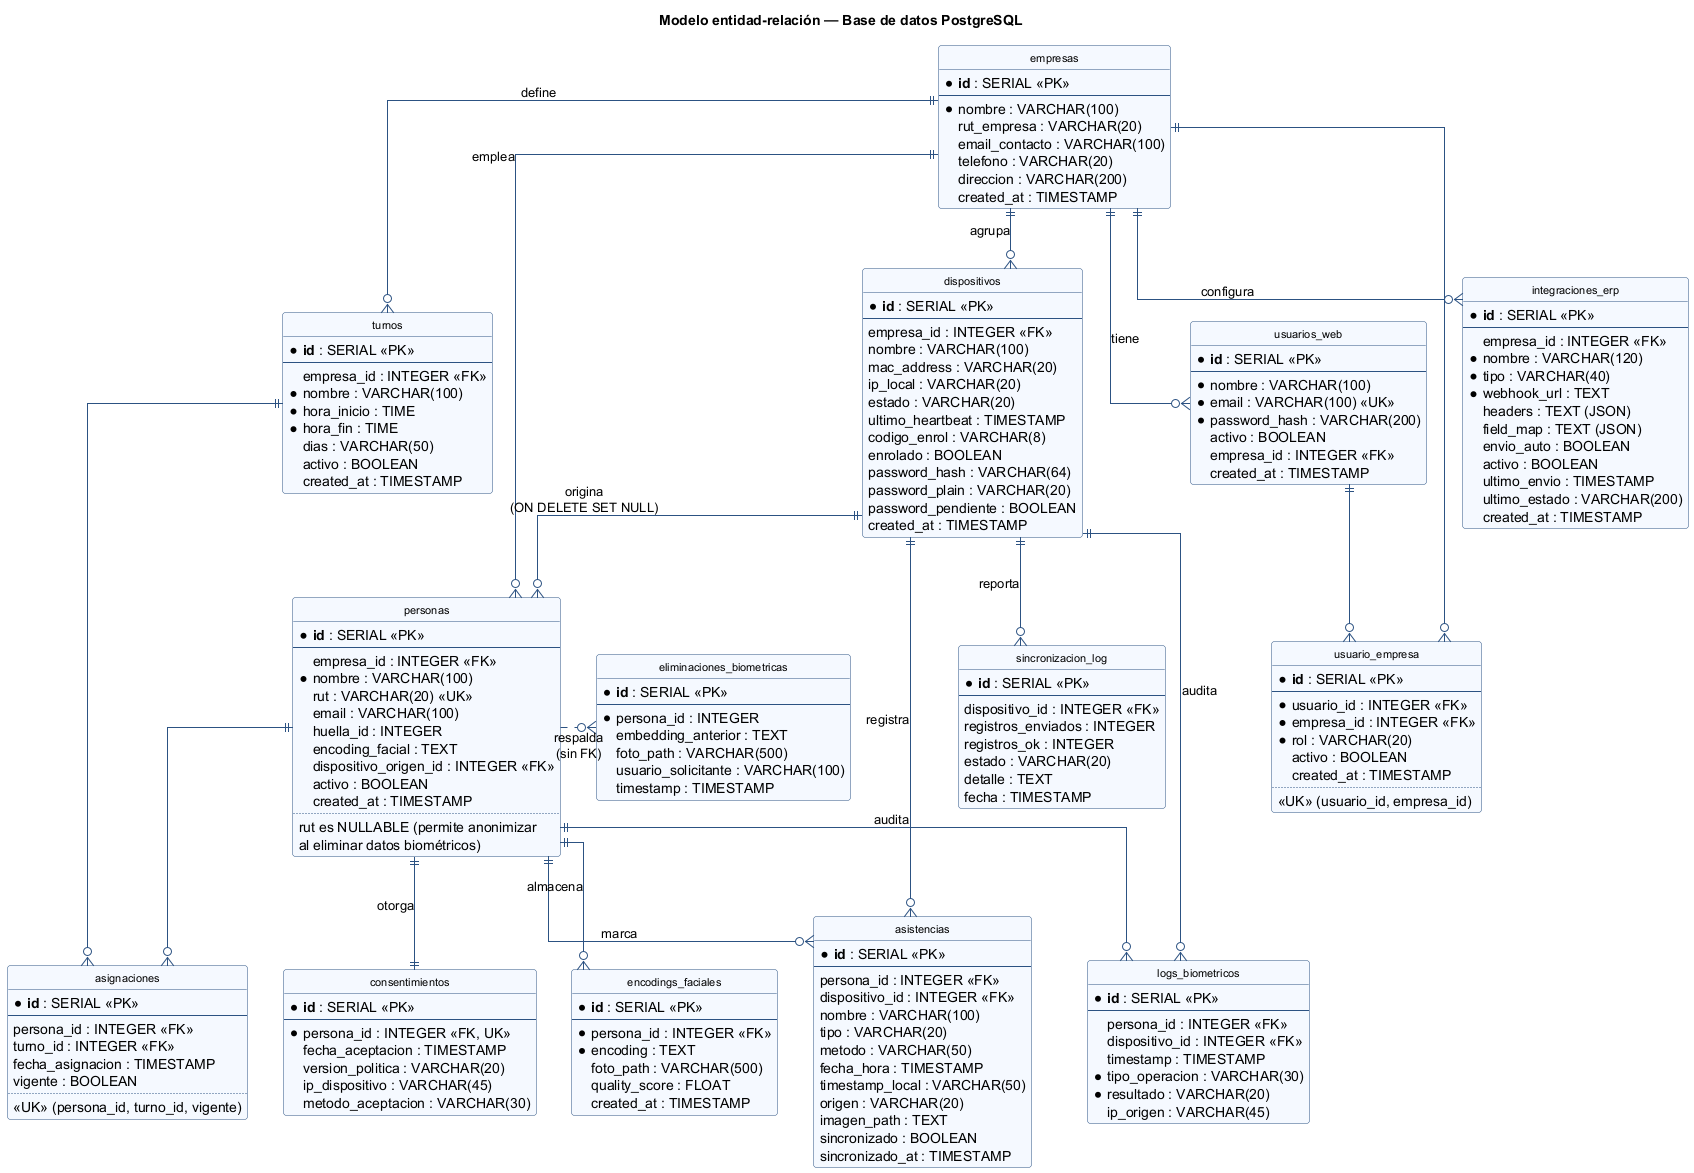
\includegraphics[width=\linewidth]{diagrams/diagrama_er_base_datos.png}
    \caption{Diagrama entidad-relación de la base de datos (14 tablas).}
    \label{fig:db-er}
\end{figure}

Las imágenes faciales, tanto las de registro como las de identificación durante la marcación, viajan del ESP32-CAM al backend por HTTP, como un JPEG crudo en formato application/octet-stream dirigido al endpoint correspondiente (POST /api/facial/registrar o POST /api/facial/identificar). El backend responde en la misma petición indicando si la foto fue aceptada, de modo que el dispositivo no necesita esperar un mensaje aparte para saber el resultado.

MQTT queda reservado para los eventos de estado del dispositivo, que son livianos y no requieren transportar una imagen. Se definen los tópicos esp32/heartbeat/<MAC> para monitorizar la actividad de los dispositivos y esp32/lwt/<MAC> para detectar desconexiones mediante el mecanismo de Last Will Testament (LWT). Para la detección activa de desconexión, se implementó el tópico esp32/ping/<MAC>: el backend publica un ping cada 30 segundos; si el ESP32-CAM no responde con un heartbeat dentro de 60 segundos, se marca como inactivo. La Figura~\ref{fig:flujo_mqtt} resume la topología de publicación y suscripción.

\begin{figure}[H]
  \centering
  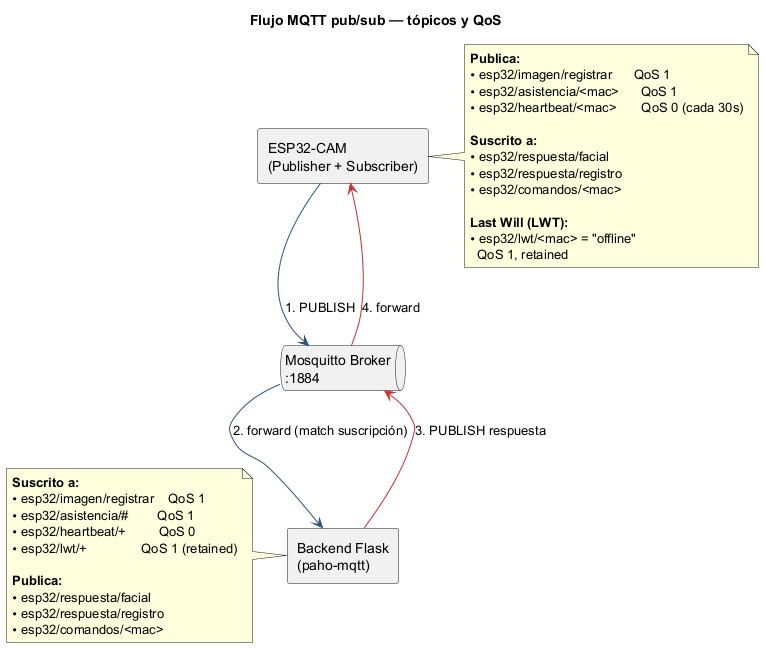
\includegraphics[width=\linewidth]{diagrams/flujo_mqtt_pub_sub.png}
  \caption{Flujo MQTT pub/sub: tópicos, direcciones y QoS entre el ESP32-CAM, el broker Mosquitto y el backend.}
  \label{fig:flujo_mqtt}
\end{figure}

\subsubsection{Implementación}

La implementación de la Iteración 3 se centró en habilitar la comunicación entre el dispositivo ESP32-CAM y el backend desarrollado en Python con Flask \cite{flask_docs}, así como en construir la base de datos PostgreSQL, accedida mediante el adaptador psycopg2 \cite{psycopg2_docs}, que soporta todo el sistema.

\paragraph{Inicialización de la base de datos}

Se implementó el módulo database.py con una función init\_db() que crea todas las tablas del sistema utilizando sentencias CREATE TABLE IF NOT EXISTS, asegurando idempotencia en los despliegues. Adicionalmente, se aplican sentencias ALTER TABLE ADD COLUMN IF NOT EXISTS para garantizar migraciones no destructivas. La función incluye la creación de índices sobre columnas frecuentemente consultadas (persona\_id, dispositivo\_id, fecha\_hora, empresa\_id) y la inserción de datos semilla (empresa por defecto, usuario administrador con contraseña hasheada).

\paragraph{Conexión Wi-Fi del ESP32-CAM y gestión de conectividad}

Para permitir la operación en red, el dispositivo implementa un mecanismo de conexión automática a Wi-Fi mediante la función tryConnectWiFi(). Esta función lee las credenciales desde wifi.json, configura el modo STA y deshabilita el ahorro de energía Wi-Fi (WIFI\_PS\_NONE) para mantener una conexión estable. La verificación continua de conectividad se realiza en verificarConexionWiFi(), que implementa un mecanismo de reintentos con backoff progresivo: tras detectar una desconexión, espera un tiempo creciente antes de reintentar (3s, 6s, 9s, 12s, 15s). Si tras 5 intentos fallidos no se logra reconectar, el dispositivo activa el Access Point como fallback.

El evento ARDUINO\_EVENT\_WIFI\_STA\_DISCONNECTED queda registrado con su código de razón y un contador de desconexiones, información expuesta a través del endpoint /wifi-diag para diagnóstico remoto.

\paragraph{Envío de imágenes faciales por HTTP: registro e identificación}

Tanto el registro como la identificación facial envían la imagen al backend de la misma manera: como JPEG crudo, sin codificarla en Base64, lo que evita el costo de procesamiento y el aumento de tamaño que implica esa codificación. Durante el registro, cuando el usuario presiona el botón de captura en la interfaz del dispositivo, el firmware toma la foto con la cámara en su calidad más alta y la sube de inmediato al backend mediante una petición POST, identificando a la persona con su RUT en una cabecera de la solicitud. El backend procesa la imagen y responde en esa misma petición si quedó aceptada o si hay que repetir la captura, lo que el dispositivo refleja en el contador de fotos de la pantalla de registro.

Durante la identificación (la consulta que ocurre al momento de marcar asistencia), el flujo es prácticamente el mismo a nivel de transporte: la imagen se captura y se envía por HTTP al endpoint de identificación, y el backend responde de forma síncrona indicando a qué persona corresponde el rostro, o un error si no encuentra coincidencia. Usar el mismo mecanismo síncrono para ambos casos simplificó el firmware, que ya no necesita dos rutas distintas para llegar al backend según el tipo de operación.

La Figura~\ref{fig:maquina_estados_esp32} ilustra la máquina de estados completa del proceso de enrolamiento biométrico en el ESP32-CAM, integrando la captura de huella digital (introducida en la Iteración 2) con el envío de la foto de referencia al backend por HTTP descrito en esta sección.

\begin{figure}[H]
  \centering
  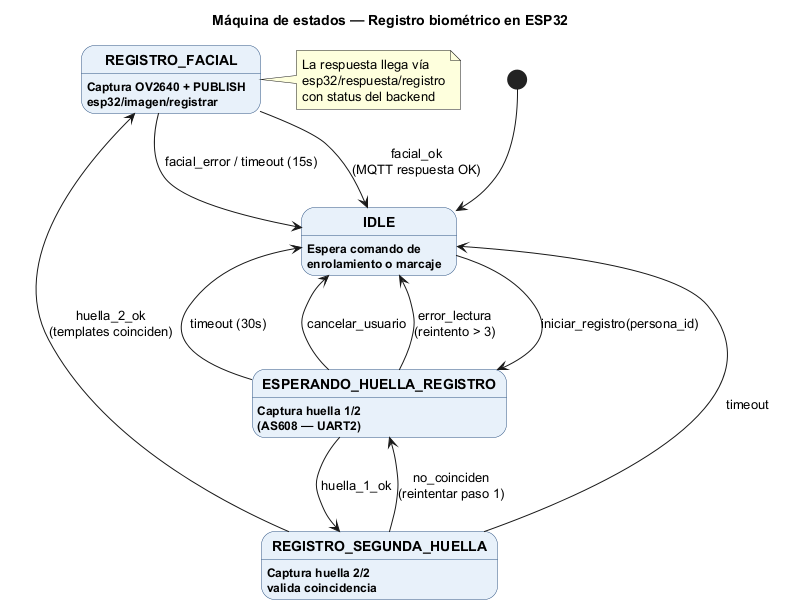
\includegraphics[width=\linewidth]{diagrams/maquina_estados_esp32.png}
  \caption{Máquina de estados del registro biométrico en el ESP32-CAM.}
  \label{fig:maquina_estados_esp32}
\end{figure}

\paragraph{Recepción de imágenes en el backend}

El backend recibe las fotos de registro e identificación a través de los endpoints REST del módulo routes/facial.py, descritos en el diseño de esta sección (ver Anexo B para el detalle completo de endpoints REST y tópicos MQTT). Al llegar una foto de registro, el backend verifica que exista consentimiento biométrico para esa persona, guarda la imagen, extrae el embedding facial y lo cifra antes de almacenarlo; si algo falla en el camino (consentimiento faltante, imagen borrosa, rostro duplicado), responde con el error correspondiente en lugar de dejar la solicitud sin respuesta.

Aparte de las imágenes, el backend mantiene un cliente MQTT para los eventos de estado del dispositivo: procesa los heartbeats, actualizando la IP y la actividad del dispositivo en la base de datos, y los mensajes de desconexión abrupta (LWT), marcándolo como inactivo. También corre en segundo plano una tarea que envía un ping cada 30 segundos a cada dispositivo enrolado, como verificación activa de que sigue en línea. Cada cambio de estado se transmite a los clientes web en tiempo real mediante streaming SSE, para que el panel se actualice sin que el administrador tenga que recargar la página.

\paragraph{Mantenimiento de la conexión MQTT en el ESP32-CAM}

El dispositivo mantiene, en paralelo a sus conexiones HTTP, un cliente MQTT que se conecta al broker si hay uno configurado y el dispositivo tiene red. Soporta URLs con esquema mqtt://, ws:// o wss:// (WebSockets seguros con TLS). Al conectarse, registra un mensaje de último aviso (LWT) para que el backend se entere si el dispositivo se cae de forma abrupta, y queda suscrito al tópico de ping para responder de inmediato cuando el backend pregunta si sigue activo. Este canal MQTT se usa únicamente para esta señalización de estado: ni el registro ni la identificación facial dependen de él.

\paragraph{Envío de datos mediante HTTP desde el ESP32-CAM}

Se implementó la capacidad del ESP32-CAM para comunicarse con la API REST del backend mediante solicitudes HTTP usando la librería HTTPClient. La función auxiliar beginHttp() configura cada petición con timeout de 10 segundos y el header X-Device-MAC para que el backend pueda identificar al dispositivo emisor. Esta función es utilizada por todos los handlers que requieren comunicación con el backend:

\begin{itemize}
    \item sincronizarPersonasDesdeBackend(): Descarga la lista completa de personas desde GET /api/personas y la persiste en personas.json.
    \item sincronizarTurnosDesdeBackend(): Descarga turnos desde GET /api/turnos.
    \item sincronizarAsignacionesDesdeBackend(): Descarga asignaciones desde GET /api/asignaciones.
    \item crearTurnoEnBackend(): Crea un turno en el backend vía POST /api/turnos.
    \item postAsistenciaEnBackend(): Envía una asistencia individual vía POST /api/asistencias.
    \item sincronizarAsistencias(): Envía un lote de asistencias pendientes vía POST /api/asistencias/sync.
\end{itemize}

\paragraph{Implementación de la API REST del backend}

El backend se implementó con Flask, organizando las rutas en blueprints independientes por dominio:
\begin{itemize}
    \item personas\_bp (routes/personas.py): CRUD de personas con validación de email, unicidad de RUT y manejo de empresa.
    \item turnos\_bp (routes/turnos.py): CRUD de turnos con filtro por empresa.
    \item asignaciones\_bp (routes/asignaciones.py): CRUD de asignaciones con verificación de pertenencia a empresa.
    \item asistencias\_bp (routes/asistencias.py): Registro de asistencias individuales y sincronización por lotes.
    \item facial\_bp (routes/facial.py): Endpoints de reconocimiento facial (registro, verificación, identificación 1:N).
    \item dispositivos\_bp (routes/dispositivos.py): Gestión y verificación de dispositivos.
    \item logs\_bp (routes/logs.py): Consulta de logs de sincronización.
    \item erp\_bp (routes/erp.py): CRUD de integraciones ERP y envío de datos.
    \item auth\_bp (routes/auth.py): Autenticación de usuarios del panel web.
\end{itemize}

Cada blueprint se registra en la aplicación Flask principal (app.py), junto con la configuración de CORS para permitir peticiones desde cualquier origen. El backend se ejecuta en el puerto 5000 con modo debug activado y recarga automática deshabilitada para evitar conflictos con el cliente MQTT.

\paragraph{Infraestructura con Docker Compose}

Para garantizar un entorno reproducible, se definió un archivo docker-compose.yml que levanta el broker Mosquitto (imagen eclipse-mosquitto:latest) con el puerto 1884 (externo, mapeado al 1883 interno) para MQTT nativo y el puerto 9001 para WebSockets expuestos, volúmenes para configuración, datos y logs persistentes, y una red bridge dedicada. El backend Flask y la base de datos PostgreSQL pueden ejecutarse en el host o en contenedores adicionales según la configuración de despliegue. La Figura~\ref{fig:docker_despliegue} presenta el diagrama de despliegue completo.

\begin{figure}[H]
  \centering
  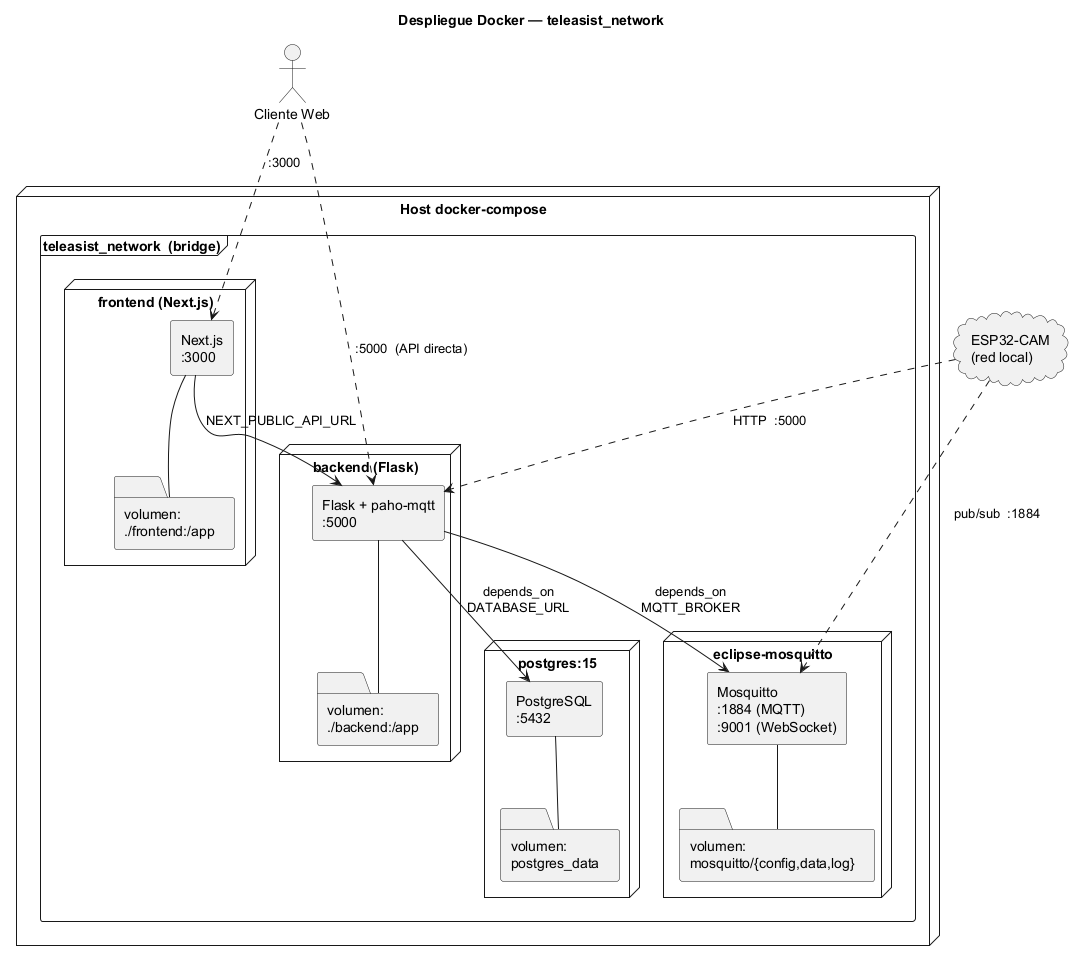
\includegraphics[width=\linewidth]{diagrams/arquitectura_despliegue_docker.png}
  \caption{Arquitectura de despliegue Docker: servicios, puertos, volúmenes y dependencias en la red.}
  \label{fig:docker_despliegue}
\end{figure}

\subsubsection{Pruebas}

Se diseñaron las siguientes pruebas para validar la comunicación y el backend:

\begin{itemize}
    \item \textbf{Prueba de conexión Wi-Fi y reconexión}: Configurar credenciales válidas en el ESP32-CAM, verificar que se conecte correctamente y obtenga una IP. Luego, apagar el router, verificar que el dispositivo detecte la desconexión mediante el evento de sistema y active el mecanismo de reintentos. Finalmente, encender el router y verificar que el dispositivo reconecte automáticamente en menos de 30 segundos.

    \item \textbf{Prueba de envío de imagen facial por HTTP}: Capturar una imagen desde el ESP32-CAM y enviarla al endpoint de registro mediante POST. Verificar que el backend reciba la imagen, la guarde en disco y responda en la misma petición indicando si la foto fue aceptada.

    \item \textbf{Prueba de heartbeat y LWT}: Verificar que, estando el ESP32-CAM conectado, el backend reciba heartbeats periódicos (cada 30 segundos) y actualice el campo ultimo\_heartbeat en la tabla dispositivos. Desconectar el dispositivo abruptamente y verificar que el mensaje LWT se publique y el backend marque el dispositivo como inactivo en menos de 10 segundos.

    \item \textbf{Prueba de ping/pong activo}: Conectar el ESP32-CAM al broker MQTT. Verificar que el backend publique esp32/ping/<MAC> periódicamente (cada 30 segundos) y que el ESP32-CAM responda con un heartbeat que contenga el campo "pong": true. Detener la conectividad del ESP32-CAM y verificar que, tras 60 segundos sin respuesta, el backend marque el dispositivo como inactivo.

    \item \textbf{Prueba de recepción de datos en backend vía HTTP}: Enviar solicitudes POST a /api/personas, /api/turnos, /api/asignaciones y /api/asistencias desde el ESP32-CAM. Verificar que cada solicitud sea procesada correctamente por el backend (código HTTP 200/201) y que los datos queden persistidos en PostgreSQL.

    \item \textbf{Prueba de sincronización por lotes}: Generar 5 marcaciones offline en el ESP32-CAM, conectar el dispositivo a la red y ejecutar la sincronización. Verificar que los 5 registros lleguen al backend vía POST /api/asistencias/sync, que se inserten correctamente y que el dispositivo marque cada registro como sincronizado = true.

    \item \textbf{Prueba de inicialización de base de datos}: Ejecutar init\_db() sobre una base de datos vacía. Verificar que se creen las 14 tablas, los índices y los datos semilla (empresa por defecto y usuario administrador) sin errores.

    \item \textbf{Prueba de latencia de transmisión}: Medir el tiempo total desde que el ESP32-CAM envía una imagen por HTTP hasta que recibe la respuesta de confirmación del backend. Se espera un tiempo menor a 5 segundos en condiciones de red local.
\end{itemize}

\paragraph{Nuevos tópicos MQTT para control y notificación}

En iteraciones posteriores se agregaron los siguientes tópicos al ecosistema MQTT:

\begin{itemize}
    \item backend/comando/<MAC>: Permite al backend enviar comandos remotos al ESP32-CAM. La función enviar\_comando\_dispositivo() en mqtt\_handler.py publica un JSON con el campo comando en este tópico.

    \item backend/notificacion/<MAC>: Utilizado por el módulo eventos\_mqtt.py para notificar a los dispositivos que deben sincronizar sus datos. Cada vez que se crea, actualiza o elimina una persona, turno o asignación, la función notificar\_sincronizacion() publica un mensaje indicando el tipo de entidad y la acción realizada.

    \item esp32/huella/resultado/<huella\_id>: Tópico en el que el ESP32-CAM publica el resultado del enrolamiento de una huella. El backend se suscribe a esp32/huella/resultado/\# y procesa la respuesta, actualizando la persona correspondiente y notificando a través de SSE.
\end{itemize}

\paragraph{Módulo eventos\_mqtt.py}

Se implementó el módulo eventos\_mqtt.py con la función notificar\_sincronizacion(empresa\_id, tipo, accion, registro\_id). Esta función consulta los dispositivos enrolados de la empresa y publica un mensaje en backend/notificacion/<MAC> por cada uno, permitiendo que los ESP32-CAM reciban notificaciones en tiempo real sobre cambios en personas, turnos y asignaciones. Es invocada desde routes/personas.py, routes/turnos.py y routes/asignaciones.py tras cada operación de creación, actualización o eliminación.

\paragraph{Streaming SSE de huellas}

Para mantener actualizados los clientes web durante el enrolamiento de huellas, se implementó el endpoint GET /sse/huellas en app.py. La función broadcast\_huella\_update() difunde los resultados del enrolamiento (recibidos por MQTT en esp32/huella/resultado/\#) a todos los clientes conectados al SSE, permitiendo que el panel web muestre en tiempo real el progreso del registro biométrico.

\subsubsection{Refinamientos posteriores}

\begin{itemize}
    \item \textbf{Decorador @requiere\_dispositivo\_enrolado}: definido en routes/auth.py, valida que el dispositivo asociado a la petición (request.dispositivo\_id) exista en la tabla dispositivos con enrolado = TRUE, devolviendo 403 en caso contrario. Se aplica sobre endpoints biométricos sensibles como /api/facial/registrar, evitando que un dispositivo no autorizado opere sobre datos biométricos.

    \item \textbf{Integridad referencial con ON DELETE SET NULL y RUT nullable}: la columna dispositivo\_origen\_id de la tabla personas (y dispositivo\_id de asistencias) se definió con REFERENCES dispositivos(id) ON DELETE SET NULL, de modo que eliminar un dispositivo no elimina en cascada las personas ni asistencias asociadas, sino que conserva el historial con la referencia en NULL. De forma análoga, la columna rut de personas se migró a nullable (ALTER TABLE personas ALTER COLUMN rut DROP NOT NULL) para permitir el borrado de datos sensibles de una persona sin perder su historial de asistencias.
\end{itemize}


%% ============================================================
%% ITERACIÓN 4: Reconocimiento facial, anti-spoofing y cifrado
%% ============================================================

\subsection{Iteración 4: Reconocimiento facial, anti-spoofing y cifrado biométrico}

Esta iteración incorpora el procesamiento biométrico en el backend: reconocimiento facial con DeepFace, validación anti-spoofing y cifrado de embeddings faciales. El sistema pasa de solo transmitir imágenes a realizar verificación e identificación biométrica.

\subsubsection{Análisis}

Para incorporar el reconocimiento facial al sistema, se evaluaron diversas librerías y modelos de deep learning. Se seleccionó DeepFace por las siguientes razones:

\begin{itemize}
    \item Soporta múltiples modelos de reconocimiento facial (Facenet, VGG-Face, ArcFace, etc.) y detectores (RetinaFace, MTCNN, OpenCV, etc.).
    \item Incluye funcionalidad de anti-spoofing integrada, capaz de distinguir entre un rostro real y una fotografía o pantalla, analizando textura, profundidad y reflectancia de la piel.
    \item Su API en Python es sencilla de integrar con Flask y compatible con las imágenes JPEG capturadas por la cámara OV2640 del ESP32-CAM.
    \item Facenet genera embeddings de 128 dimensiones, optimizando el almacenamiento y la velocidad de comparación.
\end{itemize}

Se identificaron los siguientes requisitos funcionales para esta iteración:

\begin{itemize}
    \item \textbf{Registro facial}: Recibir una imagen del ESP32-CAM, extraer el embedding facial, validar que el rostro no esté duplicado en la base de datos (detección de identidades repetidas) y almacenar el embedding cifrado.
    \item \textbf{Identificación 1:N}: Dada una imagen capturada en vivo, comparar su embedding contra todos los embeddings almacenados y retornar la identidad con mayor coincidencia, si supera el umbral de similitud.
    \item \textbf{Verificación 1:1}: Dada una imagen y un rut, verificar si la imagen corresponde a la persona declarada.
    \item \textbf{Anti-spoofing}: Detectar intentos de suplantación mediante fotografías impresas, pantallas de dispositivos o máscaras, rechazando la captura si no se detecta un rostro real.
    \item \textbf{Cifrado de embeddings}: Los vectores de características faciales (embeddings) son datos biométricos sensibles. Para protegerlos, se deben cifrar antes de persistirlos en la base de datos, utilizando una clave derivada de una variable de entorno.
    \item \textbf{Consentimiento biométrico}: Todo registro facial debe estar precedido por la aceptación explícita de una política de privacidad por parte del trabajador, en cumplimiento de la normativa de protección de datos.
\end{itemize}

\subsubsection{Diseño}

El flujo de procesamiento facial se divide en tres operaciones principales:

\begin{enumerate}
    \item \textbf{Registro} (POST /api/facial/registrar):
    \begin{itemize}
        \item Recibe la imagen como JPEG crudo (application/octet-stream) con el RUT en un header HTTP, que es como la envía el dispositivo, o como JSON con la imagen en Base64, opción que se mantiene para clientes web.
        \item Verifica que exista consentimiento biométrico en la tabla consentimientos. Si no existe, rechaza con HTTP 403.
        \item Guarda la imagen como static/previews/<id>.jpg.
        \item Aplica un \textbf{filtro de calidad de imagen} que mide la nitidez mediante la varianza del Laplaciano \cite{pech2000_laplacian}. Si la imagen es demasiado plana o borrosa (por debajo de un umbral configurable, 50 por defecto), se rechaza como posible intento de suplantación (foto de pantalla o papel) antes de llegar a DeepFace, ahorrando procesamiento innecesario del modelo.
        \item Extrae el embedding con DeepFace usando el modelo Facenet y un detector configurable mediante variable de entorno (FACIAL\_DETECTOR), utilizando MTCNN por defecto por su velocidad (tres veces más rápido que RetinaFace con precisión comparable) y sin anti-spoofing en esta etapa.
        \item Cifra el embedding con Fernet y lo almacena en la tabla encodings\_faciales, que permite acumular múltiples fotos de referencia por persona con distintos ángulos e iluminación, mejorando la precisión en subsecuentes identificaciones.
    \end{itemize}

    El flujo completo de enrolamiento biométrico, desde la creación de la persona en el panel web por parte del administrador, pasando por el registro de huella en dos pasos en el ESP32-CAM, hasta la captura facial enviada por HTTP al backend donde se extrae, cifra y almacena el embedding, se ilustra en el diagrama de secuencia de la Figura~\ref{fig:flujo_enrolamiento} del Anexo C.

    \item \textbf{Identificación 1:N} (POST /api/facial/identificar):
    \begin{itemize}
        \item Recibe la imagen como JPEG crudo (application/octet-stream) desde el ESP32-CAM, o como JSON con Base64 desde la web.
        \item Aplica el mismo filtro de calidad Laplacian como barrera anti-spoofing previa, rechazando imágenes de baja nitidez antes de invocar DeepFace.
        \item Extrae el embedding con DeepFace (anti-spoofing activado mediante anti\_spoofing=True).
        \item Consulta una caché en memoria de embeddings (con TTL configurable, 60 segundos por defecto). Si la caché expiró, recarga todos los embeddings desde la base de datos. Para cada persona, compara contra todos los embeddings almacenados en encodings\_faciales (multi-encoding) y selecciona la menor distancia. Esto mejora la precisión porque el sistema puede reconocer a un trabajador aunque la captura en vivo tenga una iluminación o ángulo diferentes a los de su foto de registro.
        \item Si la menor distancia es inferior al umbral (10.0 para Facenet), retorna el rut correspondiente. En caso contrario, retorna HTTP 404.
    \end{itemize}

    El ciclo de marcaje automático por centinela facial, en el que cada 6 segundos el ESP32-CAM evalúa el sensor PIR, captura una imagen, la envía por HTTP al endpoint de identificación, y según la respuesta del backend registra la asistencia y dispara el push asíncrono a los ERP configurados, se presenta en el diagrama de secuencia de la Figura~\ref{fig:flujo_marcaje} del Anexo C, dado su tamaño.

    \item \textbf{Verificación 1:1} (POST /api/facial/verificar):
    \begin{itemize}
        \item Recibe rut e imagen (Base64).
        \item Descifra todos los embeddings almacenados para esa persona en encodings\_faciales y extrae el embedding de la imagen capturada (con anti-spoofing activado).
        \item Calcula la distancia euclidiana contra cada embedding de referencia y selecciona la menor. Si es menor que 10.0, retorna éxito con el nivel de confianza calculado como max(0, (1 - distancia/20) * 100).
    \end{itemize}
\end{enumerate}

El modelo seleccionado es Facenet por su equilibrio entre precisión y tamaño de embedding (128 dimensiones). El detector facial es configurable mediante variable de entorno (FACIAL\_DETECTOR), utilizando MTCNN por defecto. Si bien RetinaFace ofrece mayor robustez ante variaciones extremas de pose e iluminación, MTCNN es tres veces más rápido y mantiene una precisión comparable para las condiciones típicas de una cámara de control de asistencia (rostro frontal a corta distancia), lo que lo hace más adecuado para un dispositivo embebido como el ESP32-CAM. El umbral de 10.0 para la distancia euclidiana fue elegido con base en la documentación de DeepFace y ajustes empíricos realizados durante el desarrollo.

Para el cifrado de embeddings se utiliza el algoritmo Fernet (AES-128 en modo CBC con HMAC-SHA256 para autenticación), parte de la librería cryptography de Python. La clave de cifrado se deriva aplicando SHA-256 a una variable de entorno (BIOMETRIC\_KEY), garantizando que los embeddings nunca se almacenen en texto plano en la base de datos.

\subsubsection{Implementación}

\paragraph{Procesamiento de imágenes en el backend}

El módulo routes/facial.py implementa los tres endpoints descritos en el diseño. Las funciones auxiliares incluyen:

\begin{itemize}
    \item \_validar\_calidad\_imagen(img\_path): Aplica el filtro Laplaciano (varianza del Laplaciano) sobre la imagen decodificada para medir su nitidez. Si el valor está por debajo del umbral configurable en FACIAL\_NITIDEZ\_UMBRAL (50 por defecto), la imagen se considera borrosa o plana (posible foto de pantalla o papel) y se rechaza antes de llegar a DeepFace, funcionando como una capa adicional de anti-spoofing.
    \item extraer\_embedding(img\_path, anti\_spoofing): Invoca DeepFace.represent() con el modelo Facenet pre-cargado y el detector configurable vía variable de entorno. Si anti\_spoofing=True, activa la detección de suplantación.
    \item guardar\_imagen\_de\_registro(persona\_id, imagen\_b64): Decodifica la imagen Base64, la convierte a RGB con Pillow y la guarda en static/previews/<id>.jpg.
    \item \_verificar\_consentimiento(persona\_id): Consulta la tabla consentimientos para verificar que exista un registro de aceptación.
    \item \_log\_biometrico(persona\_id, dispositivo\_id, tipo\_operacion, resultado): Inserta un registro de auditoría en logs\_biometricos.
\end{itemize}

Además, para optimizar el rendimiento, el modelo Facenet se precarga al iniciar el servidor mediante DeepFace.build\_model('Facenet', task='facial\_recognition'), eliminando la latencia de carga de pesos en la primera solicitud. Los embeddings almacenados en la base de datos se mantienen en una caché en memoria con tiempo de vida configurable (por defecto 60 segundos, mediante FACIAL\_CACHE\_TTL), evitando consultas repetitivas y descifrados a la base de datos en cada identificación. La caché se invalida automáticamente al registrar una nueva foto o al eliminar datos biométricos, garantizando consistencia.

\paragraph{Cifrado y descifrado de embeddings}

El módulo encryption.py proporciona dos funciones:

\begin{itemize}
    \item cifrar\_embedding(embedding): Serializa el embedding como JSON, lo cifra con Fernet y codifica el resultado en Base64 URL-safe.
    \item descifrar\_embedding(cifrado\_str): Decodifica el Base64, descifra con Fernet y deserializa el JSON para obtener el vector original.
\end{itemize}

% =====================================================================
% Diagrama 8 — Pipeline de cifrado biométrico (TikZ)
% Incluir en memoria.tex con:  \input{diagrams/08_pipeline_cifrado_biometrico.tex}
% Requiere en el preámbulo: \usepackage{tikz}
%                           \usetikzlibrary{arrows.meta, positioning, shapes.geometric}
% =====================================================================
\begin{figure}[H]
\centering
\begin{tikzpicture}[
  node distance=1.1cm and 1.3cm,
  every node/.style={font=\small},
  box/.style={draw, rounded corners=3pt, minimum height=1.1cm,
              minimum width=2.7cm, align=center, fill=blue!8,
              drop shadow={opacity=0.15}},
  crypto/.style={draw, rounded corners=3pt, minimum height=1.1cm,
                 minimum width=2.7cm, align=center, fill=orange!20,
                 drop shadow={opacity=0.15}},
  db/.style={draw, cylinder, shape border rotate=90, aspect=0.25,
             minimum height=1.5cm, minimum width=2.5cm,
             align=center, fill=gray!15},
  fallback/.style={draw, dashed, rounded corners=3pt, minimum height=1.0cm,
                   minimum width=2.7cm, align=center, fill=red!8},
  arrow/.style={-{Stealth[length=2.5mm]}, thick},
  darrow/.style={-{Stealth[length=2.5mm]}, thick, dashed, gray!70!black},
  lbl/.style={font=\scriptsize\itshape, text=gray!50!black}
]

% --- Fila superior: cifrado ---
\node[box]                       (emb)    {Embedding\\\scriptsize{\texttt{float[512]}}};
\node[crypto, right=of emb]      (cif)    {\texttt{cifrar\_embedding()}};
\node[crypto, right=of cif]      (fernet) {Fernet\\\scriptsize{AES-128-CBC + HMAC-SHA256}};
\node[db,     right=of fernet]   (dbn)    {PostgreSQL\\\scriptsize{TEXT (base64)}};

% --- Fila inferior: descifrado ---
\node[crypto, below=1.7cm of fernet] (dcif)    {\texttt{descifrar\_embedding()}};
\node[box,    left=of dcif]          (compare) {Comparación\\\scriptsize{DeepFace.verify}};

% --- Fallback ---
\node[fallback, below=0.7cm of dbn] (legacy) {Fallback legacy\\\scriptsize{embedding sin cifrar}};

% --- Flechas principales ---
\draw[arrow] (emb)    -- (cif);
\draw[arrow] (cif)    -- (fernet);
\draw[arrow] (fernet) -- (dbn);
\draw[arrow] (dbn)    |- (dcif);
\draw[arrow] (dcif)   -- (compare);

% --- Camino fallback ---
\draw[darrow] (legacy.west) -| ([xshift=-0.3cm]dcif.south)
              node[pos=0.75, below, font=\scriptsize] {parse directo};

% --- Etiquetas ---
\node[lbl, above=0.1cm of cif] {clave Fernet (\texttt{.env})};
\node[lbl, above=0.1cm of dcif] {misma clave (rotable)};

\end{tikzpicture}
\caption[Pipeline de cifrado biométrico]{Pipeline de cifrado biométrico — Fernet (AES-128-CBC + HMAC-SHA256) con fallback para embeddings legacy almacenados sin cifrar.}
\label{fig:pipeline_cifrado_biometrico}
\end{figure}


\paragraph{Actualización y eliminación de datos faciales}

Se implementó el endpoint PUT /api/facial/actualizar/<persona\_id> que permite reemplazar el embedding y la foto de una persona existente. También se implementó DELETE /api/personas/<id>/datos-biometricos que elimina el embedding facial, la huella asociada, la foto en disco y el consentimiento, pero conserva los registros de asistencia históricos. La eliminación queda registrada en la tabla eliminaciones\_biometricas para trazabilidad.

Se implementó además el endpoint POST /api/facial/agregar-foto que permite agregar fotos de referencia adicionales a una persona ya registrada, sin reemplazar las existentes. Cada nueva foto pasa por el mismo filtro de calidad Laplacian y se almacena como un nuevo registro en encodings\_faciales. Esta funcionalidad de enrolamiento progresivo permite mejorar la precisión del sistema a lo largo del tiempo: si un trabajador experimenta falsos rechazos, se le pueden agregar más fotos de referencia con distintos ángulos o condiciones de iluminación, aumentando la robustez del reconocimiento sin necesidad de rehacer el registro completo.

\subsubsection{Pruebas}

Se diseñaron las siguientes pruebas para validar el módulo de reconocimiento facial:

\begin{itemize}
    \item \textbf{Prueba de registro facial exitoso}: Enviar una imagen facial válida junto con un rut que tenga consentimiento registrado. Verificar que el backend extraiga el embedding, lo almacene cifrado y responda con HTTP 200.

    \item \textbf{Prueba de detección de duplicados}: Registrar una segunda imagen del mismo rostro para otra persona. Verificar que el backend detecte la similitud (distancia < 10.0) y rechace el registro con HTTP 409, indicando el nombre de la persona con la que coincide.

    \item \textbf{Prueba de rechazo por falta de consentimiento}: Intentar registrar un rostro para una persona sin consentimiento biométrico. Verificar que el backend rechace la operación con HTTP 403.

    \item \textbf{Prueba de identificación 1:N}: Registrar 3 personas con sus respectivas fotos. Enviar una nueva foto de una de ellas al endpoint de identificación. Verificar que el backend retorne el rut correcto.

    \item \textbf{Prueba de identificación con rostro desconocido}: Enviar una foto de una persona no registrada. Verificar que el backend retorne HTTP 404 y registre el intento fallido en logs\_biometricos.

    \item \textbf{Prueba de anti-spoofing con fotografía impresa}: Capturar una foto de un rostro registrado desde una pantalla o impresión y enviarla al endpoint de identificación. Verificar que DeepFace con anti\_spoofing=True rechace la imagen por no detectar un rostro real (excepción ValueError con mensaje ``Spoof detected'').

    \item \textbf{Prueba de resistencia a condiciones de iluminación}: Capturar imágenes del mismo rostro bajo 3 condiciones de iluminación (luz natural, luz artificial tenue, contraluz). Verificar que los 3 embeddings generados mantengan distancia euclidiana entre sí menor a 10.0 y que el sistema identifique correctamente a la persona.

    \item \textbf{Prueba de cifrado y descifrado}: Almacenar un embedding en la base de datos y verificar que el valor en la columna encoding\_facial no sea legible (no contenga los números del vector en texto plano). Luego, recuperar el registro y descifrar el embedding; verificar que el vector original se reconstruya idénticamente.

    \item \textbf{Prueba de eliminación de datos biométricos}: Ejecutar el endpoint de eliminación de datos biométricos para una persona con rostro registrado. Verificar que el embedding se elimine de la base de datos, que la foto se borre del disco, que el consentimiento se elimine, que los registros de asistencia se conserven y que quede una entrada en eliminaciones\_biometricas.

    \item \textbf{Prueba de filtro de calidad de imagen}: Enviar al endpoint de registro una imagen deliberadamente borrosa o una foto de una pantalla (baja varianza de Laplacian). Verificar que el backend rechace la imagen antes de invocar DeepFace, retornando un error de calidad insuficiente.

    \item \textbf{Prueba de múltiples fotos de referencia}: Registrar una persona con una foto frontal. Luego, agregar una segunda foto de la misma persona con distinto ángulo mediante POST /api/facial/agregar-foto. Realizar una identificación con una tercera foto y verificar que el sistema reconozca a la persona correctamente, comparando contra ambos embeddings de referencia.
    
    \item \textbf{Prueba de caché de embeddings}: Realizar una identificación exitosa y verificar los tiempos de respuesta. Realizar una segunda identificación inmediatamente después; verificar que el tiempo sea significativamente menor porque los embeddings se sirvieron desde la caché en memoria sin consultar la base de datos.
\end{itemize}

\paragraph{Endpoint identificar-o-registrar}

Se implementó el endpoint POST /api/facial/identificar-o-registrar que combina ambos flujos en una sola llamada: primero intenta identificar a la persona por su rostro; si la identificación es exitosa, retorna los datos de la persona; si falla y se proporciona un RUT con consentimiento biométrico, registra automáticamente la nueva persona con el embedding facial extraído. Este endpoint facilita el enrolamiento progresivo en el dispositivo: un trabajador puede colocarse frente al ESP32-CAM y, si ya está registrado, se marca su asistencia; si no, el sistema lo registra sobre la marcha. El endpoint incluye validación de calidad de imagen, anti-spoofing y log biométrico tanto para identificación como para registro.

\subsubsection{Refinamientos posteriores}

\begin{itemize}
    \item \textbf{Transmisión de imágenes vía octet-stream}: el envío de la imagen facial migró de un esquema basado en JSON con la foto codificada en Base64 a un envío binario directo (Content-Type: application/octet-stream) con el RUT o la MAC del dispositivo en un header HTTP (X-RUT / X-Device-MAC). El backend mantiene compatibilidad retroactiva con el formato Base64 como \textit{fallback}. El cambio elimina el overhead de codificación Base64 (aproximadamente 33\% de tamaño adicional) y simplifica el firmware, que ahora envía directamente el buffer JPEG capturado por la cámara (fb->buf, fb->len).

    \item \textbf{Captura de 3 fotos de referencia por persona}: el flujo de registro se extendió de una sola foto a tres capturas sucesivas (FOTOS\_REQUERIDAS = 3 en el firmware), idealmente frontal y de ambos perfiles, generando tres embeddings independientes almacenados en la tabla encodings\_faciales. Esto mejora la tasa de identificación ante variaciones de ángulo o iluminación, ya que la comparación 1:N evalúa contra todos los embeddings de referencia disponibles.
\end{itemize}


%% ============================================================
%% ITERACIÓN 5: Autenticación, multi-tenant y enrolamiento
%% ============================================================

\subsection{Iteración 5: Autenticación, multi-tenant y enrolamiento de dispositivos}

La quinta iteración incorpora la capa de seguridad y administración del sistema: autenticación de usuarios del panel web mediante JWT, un modelo multi-tenant que permite a múltiples empresas operar sobre la misma instancia del backend con datos aislados, y un mecanismo seguro de enrolamiento de dispositivos ESP32-CAM mediante PIN de un solo uso.

\subsubsection{Análisis}

El sistema, al estar orientado a un entorno empresarial, requiere que diferentes organizaciones puedan utilizar la misma plataforma sin que sus datos se mezclen. Asimismo, el panel web administrativo debe restringir el acceso según el rol del usuario. Finalmente, cada dispositivo ESP32-CAM debe ser vinculado de forma segura a una empresa específica, evitando que dispositivos no autorizados inyecten datos en el sistema.

Los requisitos identificados son:

\begin{itemize}
    \item \textbf{Multi-tenant}: Cada entidad (persona, turno, asignación, asistencia, dispositivo) debe pertenecer a una empresa. Las consultas deben filtrarse por empresa según el contexto del usuario autenticado. El administrador global (rol admin) tiene visibilidad sobre todas las empresas.
    \item \textbf{Autenticación JWT}: El panel web backend debe requerir autenticación para operaciones sensibles. Los tokens JWT (JSON Web Tokens), firmados con HMAC-SHA256, transportan el ID de usuario, la empresa seleccionada y su rol. Tienen expiración de 24 horas.
    \item \textbf{Roles de usuario}: Se definen tres roles jerárquicos:
    \begin{itemize}
        \item admin: Acceso total al sistema, puede crear empresas, gestionar todos los usuarios y dispositivos.
        \item empleador: Acceso limitado a los datos de su empresa; puede gestionar trabajadores, turnos y ver asistencias.
        \item trabajador: Acceso restringido a sus propios datos de asistencia.
    \end{itemize}
    \item \textbf{Enrolamiento de dispositivos}: Un administrador genera un PIN de 8 caracteres en el panel web. Ese PIN se ingresa en el ESP32-CAM (vía web embebida), que lo envía al backend junto con su MAC address. Si el PIN es válido y no ha sido usado, el dispositivo queda enrolado y asociado a la empresa correspondiente.
    \item \textbf{Auto-registro de empresas}: Se requiere un endpoint público que permita a una nueva organización registrarse de forma autónoma en el sistema, sin intervención del administrador central. La empresa proporciona sus datos (nombre, RUT, email, etc.) y los datos del usuario administrador; el sistema crea la empresa, el usuario, y la asociación entre ambos con rol admin en una sola transacción atómica, retornando un token JWT para que el nuevo administrador quede autenticado inmediatamente. Esto facilita el despliegue del sistema en nuevos clientes sin requerir configuración manual previa.
    \item \textbf{Monitorización de dispositivos}: Una vez enrolado, el ESP32-CAM envía heartbeats periódicos vía MQTT. El backend actualiza el estado del dispositivo (activo) y registra su última actividad. Un proceso watchdog marca como inactivo a los dispositivos que no han enviado heartbeat en más de 90 segundos.
\end{itemize}

\subsubsection{Diseño}

\paragraph{Modelo de datos multi-tenant}

La estrategia multi-tenant se implementa a nivel de base de datos mediante una columna empresa\_id en las tablas personas, turnos, dispositivos, integraciones\_erp y asistencias (esta última a través de la relación con personas). La tabla empresas actúa como entidad raíz del tenant. La tabla asociativa usuario\_empresa vincula usuarios con empresas y define el rol que cada usuario tiene en cada empresa, permitiendo que un mismo usuario tenga roles distintos en diferentes organizaciones.

\paragraph{Flujo de autenticación}

\begin{enumerate}
    \item El usuario envía email y contraseña al endpoint POST /api/auth/login.
    \item El backend valida las credenciales contra la tabla usuarios\_web usando bcrypt.
    \item Se consultan las empresas asociadas al usuario en usuario\_empresa.
    \item Si el usuario pertenece a una sola empresa, se selecciona automáticamente. Si pertenece a varias, se retorna la lista para que elija.
    \item Se genera un token JWT con payload: user\_id, empresa\_id, rol, persona\_id (si es trabajador) y exp (24 horas).
    \item Las peticiones subsecuentes deben incluir el header Authorization: Bearer <token>.
\end{enumerate}

Se implementan dos niveles de protección para los endpoints:
\begin{itemize}
    \item @token\_required: Exige token JWT válido.
    \item @requiere\_rol('admin', 'empleador'): Además del token, exige que el rol del usuario esté en la lista permitida.
    \item @token\_opcional: Intenta extraer el token si está presente; si no, permite el acceso sin autenticación (útil para endpoints consumidos por el ESP32-CAM, que en su lugar envían el header X-Device-MAC para identificar la empresa).
\end{itemize}

\begin{figure}[H]
  \centering
  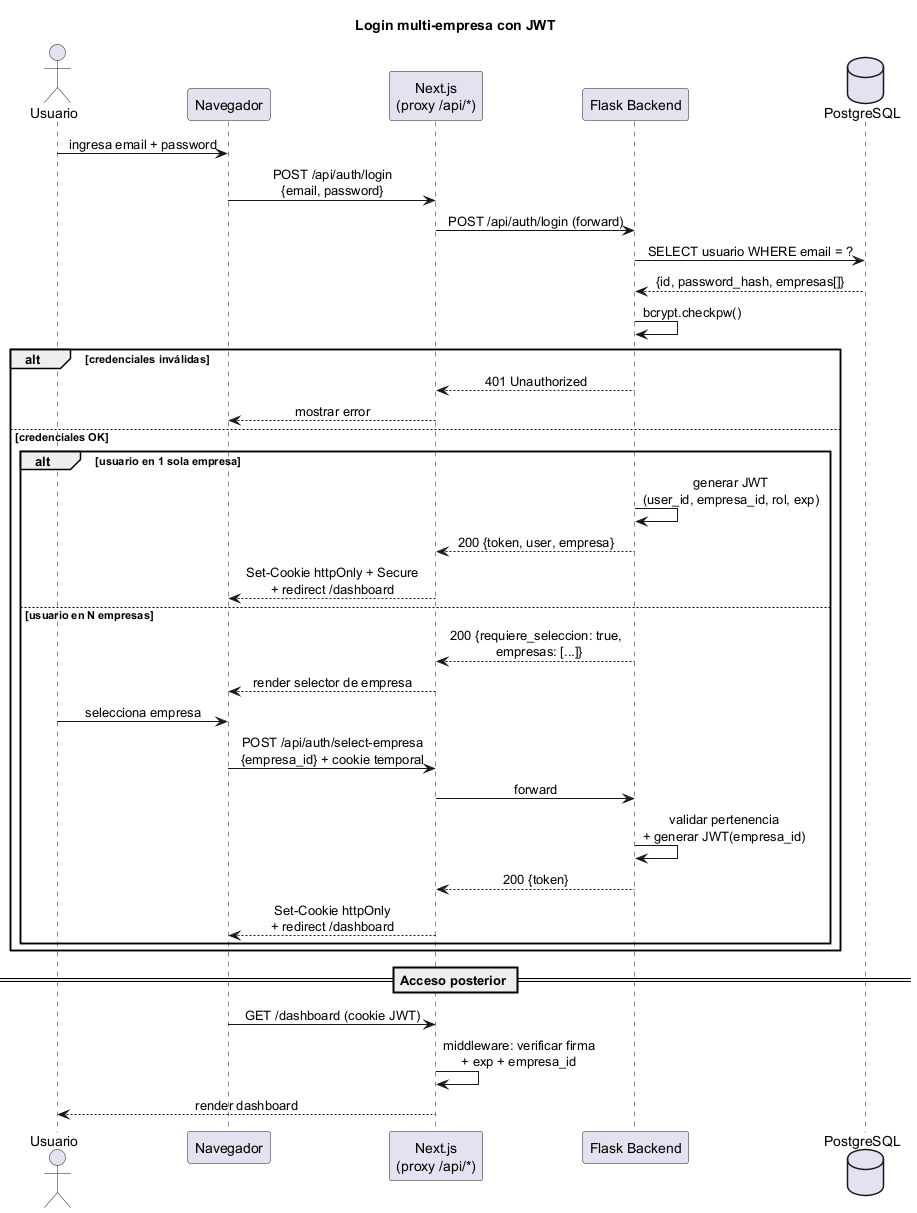
\includegraphics[width=0.95\linewidth]{diagrams/flujo_login_jwt.png}
  \caption{Diagrama de secuencia del login multi-empresa con JWT.}
  \label{fig:flujo_login_jwt}
\end{figure}

\paragraph{Flujo de enrolamiento de dispositivos}

\begin{enumerate}
    \item Un administrador o empleador accede a POST /api/dispositivos/generar-pin desde el panel web, especificando un nombre para el dispositivo. El backend genera un PIN alfanumérico de 8 caracteres (ej. A3B9XK2M) usando secrets.choice() y lo inserta en la tabla dispositivos con enrolado = FALSE.
    \item El administrador ingresa el PIN en la interfaz web del ESP32-CAM (/wifi-setup).
    \item Al guardar la configuración, el ESP32-CAM envía POST /api/dispositivos/enrolar con el PIN, su MAC address y su IP local.
    \item El backend valida el PIN, asocia la MAC y la IP al dispositivo, marca enrolado = TRUE y limpia el PIN para que no pueda ser reutilizado.
    \item A partir de este momento, el ESP32-CAM envía heartbeats periódicos y el backend lo reconoce como dispositivo autorizado de la empresa.
\end{enumerate}

\paragraph{Heartbeat y Last Will Testament (LWT)}

El ESP32-CAM publica periódicamente (cada 30 segundos) un mensaje JSON en el tópico esp32/heartbeat/<MAC> con su MAC, timestamp e IP. El backend actualiza el campo ultimo\_heartbeat y marca el estado como activo. Al conectarse al broker MQTT, el ESP32-CAM configura un mensaje LWT en el tópico esp32/lwt/<MAC> con \{"estado": "inactivo"\}. Si el dispositivo se desconecta abruptamente, el broker publica automáticamente el LWT, y el backend marca el dispositivo como inactivo.

Además del LWT y el watchdog pasivo, se implementó un ping activo como tercera capa de detección: un hilo device\_pinger() publica periódicamente (cada 30 segundos) un mensaje en el tópico esp32/ping/<MAC>. El ESP32-CAM, al recibirlo, responde inmediatamente publicando un heartbeat con el campo "pong": true. Si el backend no recibe respuesta dentro de 60 segundos, marca el dispositivo como inactivo. Este mecanismo permite detectar desconexiones incluso cuando el mensaje LWT no llega al broker (por ejemplo, por pérdida abrupta de conectividad de red). Adicionalmente, un hilo device\_watchdog ejecutado cada 60 segundos verifica qué dispositivos no han enviado heartbeat en más de 90 segundos y los marca como inactivos, constituyendo una capa de respaldo adicional.

\subsubsection{Implementación}

\paragraph{Módulo de autenticación}

El módulo routes/auth.py implementa:

\begin{itemize}
    \item login(): Valida credenciales con bcrypt, determina la empresa (con selección múltiple si aplica), vincula al trabajador con su persona\_id si el rol es trabajador, y genera el token JWT.
    \item register(): Permite a administradores y empleadores crear nuevos usuarios, asignándoles rol y empresa. Si el email ya existe, se agrega la nueva asociación usuario\_empresa en lugar de duplicar el usuario.
    \item me(): Retorna los datos del usuario autenticado, incluyendo sus empresas y rol actual.
    \item cambiar\_password(): Permite al usuario cambiar su contraseña validando la actual.
    \item generar\_pin\_enrolamiento(): Crea un PIN para enrolar un nuevo dispositivo.
    \item enrolar\_dispositivo(): Valida el PIN y completa el enrolamiento del ESP32-CAM.
    \item listar\_usuarios(), eliminar\_usuario(), listar\_empresas(), crear\_empresa(): Operaciones administrativas con control de roles.
    \item register\_company(): Endpoint público POST /api/auth/register-company que permite el auto-registro de una nueva empresa. Recibe los datos de la organización (nombre, RUT, email, teléfono, dirección) y del usuario administrador (nombre, email, contraseña). En una única transacción atómica crea la empresa, el usuario con hash bcrypt, y la asociación usuario\_empresa con rol admin. Retorna un token JWT para autenticar inmediatamente al nuevo administrador.
\end{itemize}

Los decoradores @token\_required, @token\_opcional y @requiere\_rol se definen en el mismo módulo. El decorador @token\_opcional incluye lógica para inferir la empresa a partir del header X-Device-MAC cuando no hay token JWT presente, buscando la MAC en la tabla de dispositivos. Si la MAC no existe, automáticamente crea un nuevo registro en dispositivos con estado pendiente, lo que permite que los ESP32-CAM comiencen a enviar datos incluso antes de ser formalmente enrolados.

\paragraph{Gestión de dispositivos}

El módulo routes/dispositivos.py implementa:

\begin{itemize}
    \item GET /api/dispositivos: Lista los dispositivos con su estado, MAC, IP y empresa.
    \item PUT /api/dispositivos/<id>: Actualiza el nombre del dispositivo.
    \item DELETE /api/dispositivos/<id>: Elimina un dispositivo (admin) o lo desvincula de la empresa (empleador).
    \item POST /api/dispositivos/verificar: Prueba conectividad con un dispositivo dada su IP, consultando el endpoint /estado del ESP32-CAM.
\end{itemize}

\paragraph{Monitorización vía MQTT}

En el módulo mqtt\_handler.py, la función on\_message maneja los tópicos de heartbeat y LWT:

\begin{itemize}
    \item esp32/heartbeat/<MAC>: Actualiza ultimo\_heartbeat, estado = 'activo' y opcionalmente ip\_local del dispositivo.
    \item esp32/lwt/<MAC>: Marca estado = 'inactivo' en la base de datos.
\end{itemize}

El watchdog (device\_watchdog) ejecuta un barrido inicial al arrancar (todos los dispositivos se marcan inactivos hasta que envíen su primer heartbeat) y luego verifica cada 60 segundos los heartbeats vencidos.

\subsubsection{Pruebas}

Se diseñaron las siguientes pruebas para validar la autenticación, el multi-tenant y el enrolamiento:

\begin{itemize}
    \item \textbf{Prueba de login exitoso}: Enviar credenciales válidas del administrador por defecto (admin@empresa.cl / admin123). Verificar que se reciba un token JWT, los datos del usuario y su empresa. Decodificar el token y verificar que contenga user\_id, empresa\_id y rol = admin.

    \item \textbf{Prueba de login con múltiples empresas}: Crear una segunda empresa y asignar el mismo usuario a ella con rol empleador. Iniciar sesión sin especificar empresa. Verificar que el backend retorne la lista de empresas disponibles. Luego, iniciar sesión especificando una empresa y verificar que el token refleje esa selección.

    \item \textbf{Prueba de rechazo de credenciales inválidas}: Intentar login con contraseña incorrecta. Verificar HTTP 401 y mensaje ``Credenciales inválidas''.

    \item \textbf{Prueba de acceso sin token}: Intentar acceder a GET /api/personas sin enviar header Authorization, desde un cliente sin X-Device-MAC. Verificar que el endpoint responda correctamente (acceso público o con datos limitados según el decorador).

    \item \textbf{Prueba de acceso con rol insuficiente}: Autenticarse como trabajador e intentar crear un turno (POST /api/turnos). Verificar HTTP 403 y mensaje ``Permisos insuficientes''.

    \item \textbf{Prueba de aislamiento multi-tenant}: Crear dos empresas (A y B), registrar una persona en cada una. Autenticarse como empleador de la empresa A y solicitar GET /api/personas. Verificar que solo se retornen las personas de la empresa A.

    \item \textbf{Prueba de generación de PIN}: Autenticarse como empleador y solicitar POST /api/dispositivos/generar-pin. Verificar que se reciba un PIN de 8 caracteres alfanuméricos y que en la base de datos exista un dispositivo con enrolado = FALSE.

    \item \textbf{Prueba de enrolamiento exitoso}: Con un PIN generado, enviar POST /api/dispositivos/enrolar con el PIN, una MAC y una IP. Verificar que el backend marque el dispositivo como enrolado, asocie la MAC y limpie el PIN. Verificar que el mismo PIN no pueda usarse una segunda vez (HTTP 409).

    \item \textbf{Prueba de heartbeat y estado}: Simular heartbeats desde un dispositivo enrolado. Verificar que el estado en la base de datos sea activo. Detener los heartbeats por más de 90 segundos y verificar que el watchdog marque el dispositivo como inactivo.

    \item \textbf{Prueba de LWT}: Conectar el ESP32-CAM al broker MQTT, verificar que el backend reciba el heartbeat y lo marque activo. Desconectar el dispositivo abruptamente (corte de energía). Verificar que el broker publique el LWT y el backend actualice el estado a inactivo en menos de 10 segundos.

    \item \textbf{Prueba de auto-registro de empresa}: Enviar una solicitud a POST /api/auth/register-company con los datos de una nueva empresa y su administrador. Verificar que se cree la empresa en la base de datos, que el usuario administrador se cree con contraseña encriptada (bcrypt), que exista la asociación usuario\_empresa con rol admin, y que el backend retorne un token JWT válido que permita acceder a endpoints protegidos. Verificar que un segundo intento con el mismo email de administrador retorne HTTP 409 (Conflicto).
\end{itemize}

\subsubsection{Refinamientos posteriores}

\begin{itemize}
    \item "\textbf{token\_opcional}": el decorador token\_opcional, que permite que un mismo endpoint acepte tanto usuarios web autenticados por JWT como dispositivos ESP32 identificados por el header X-Device-MAC, inicialmente creaba un registro nuevo en dispositivos si la MAC no existía en la base de datos. Este comportamiento se eliminó: ahora el decorador únicamente busca y vincula dispositivos ya existentes, dejando la creación exclusivamente al flujo explícito de enrolamiento con PIN. El cambio cierra una vía por la que un dispositivo no autorizado podía aparecer en el sistema sin pasar por el control del administrador o empleador.

    \item \textbf{PIN de enrolamiento por empresa}: la generación de PIN (POST /api/auth/dispositivos/generar-pin) quedó condicionada al rol de quien la solicita: un administrador puede generar el PIN para cualquier empresa indicada en la petición, mientras que un empleador solo puede generarlo para la empresa a la que pertenece (request.empresa\_id). El dispositivo creado queda asociado a esa empresa desde el momento de la generación del PIN, reforzando el aislamiento multi-tenant también a nivel de hardware enrolado.
\end{itemize}


%% ============================================================
%% ITERACIÓN 6: Módulo antifraude y validación previa a la captura
%% ============================================================

\subsection{Iteración 6: Módulo antifraude y validación previa a la captura}

Esta iteración implementa la prevención de suplantación de identidad en el ESP32-CAM mediante detección física de presencia, control de iluminación y procesamiento biométrico. Si bien el plan original contemplaba un sensor infrarrojo (IR) dedicado para detectar intentos de suplantación con fotografías, el enfoque implementado evolucionó hacia una solución de múltiples capas que resultó más robusta y prescindió del sensor IR adicional.

\subsubsection{Análisis}

El análisis de escenarios de suplantación identificó los siguientes vectores de ataque potenciales contra el sistema de reconocimiento facial del ESP32-CAM:

\begin{itemize}
    \item \textbf{Fotografía impresa}: Un atacante presenta una foto del rostro de un trabajador legítimo frente a la cámara.
    \item \textbf{Pantalla de dispositivo}: Un atacante muestra un video o imagen del trabajador en la pantalla de un teléfono o tablet.
    \item \textbf{Ausencia de presencia real}: La cámara captura sin que haya una persona físicamente frente al dispositivo (falsos positivos del sensor de movimiento).
\end{itemize}

Inicialmente se planificó el uso de un sensor IR dedicado que permitiera detectar la presencia de un rostro real mediante la emisión y recepción de luz infrarroja, cuya reflectancia difiere entre piel humana y superficies planas como papel o pantallas. Sin embargo, durante el desarrollo se identificaron dos factores que motivaron el cambio de estrategia:

\begin{enumerate}
    \item \textbf{Disponibilidad de GPIO}: El ESP32-CAM tiene una cantidad muy limitada de pines GPIO disponibles tras la asignación del bus paralelo de la cámara. Destinar un pin adicional al sensor IR hubiera requerido sacrificar otra funcionalidad (como el sensor PIR de presencia o el control PWM del flash).

    \item \textbf{Madurez del anti-spoofing por software}: DeepFace, la librería seleccionada para el reconocimiento facial, incorpora un detector de suplantación (\textbf{anti-spoofing}) basado en redes neuronales convolucionales que analiza micro-texturas, reflectancia de la piel y profundidad en la imagen capturada. Este detector es capaz de distinguir entre un rostro real tridimensional y una superficie plana (foto, pantalla) con una precisión comparable o superior a la de sensores IR de bajo costo como los inicialmente considerados.
\end{enumerate}

En consecuencia, se adoptó un enfoque de múltiples capas que combina:

\begin{enumerate}
    \item \textbf{Detección física de presencia (PIR)}: Un sensor infrarrojo pasivo (PIR) que detecta el calor corporal, activando el sistema de captura solo cuando hay una persona real frente al dispositivo. Esto elimina falsos positivos del software y reduce el consumo energético del sensor de huella y la cámara.
    \item \textbf{Iluminación controlada (flash PWM)}: Un destello breve y de intensidad moderada (50\% de duty cycle a 5 kHz) que ilumina el rostro durante la captura sin enceguecer a la persona. La respuesta del rostro real a esta fuente de luz puntual difiere de la de una superficie plana, aportando una capa adicional de discriminación.
    \item \textbf{Anti-spoofing por software (DeepFace)}: La capa más potente, que analiza la imagen capturada con un modelo entrenado para detectar intentos de suplantación. Las imágenes que no superan esta validación son rechazadas con una excepción ValueError que el backend traduce en un mensaje de error al ESP32-CAM.
\end{enumerate}

\subsubsection{Diseño}

\paragraph{Sensor PIR como portero del reconocimiento facial}

El lector de huellas se revisa de forma continua, sin depender del PIR: cada 500 milisegundos el sistema consulta al AS608 por si hay un dedo apoyado, de modo que una marcación por huella responda de inmediato sin esperar a que algo más la habilite. El PIR conectado al GPIO12 cumple un rol distinto, acotado al reconocimiento facial: mientras no detecta movimiento, la cámara no se usa para buscar un rostro. Al detectar movimiento (un cambio en la radiación infrarroja del entorno), el sistema enciende el flash a baja intensidad, marca que hay alguien frente al dispositivo y, si en ese momento había un bloqueo temporal del menú activo, lo anula, dando prioridad a la persona que se presentó físicamente. Tras una breve pausa de 800 milisegundos para que la lectura del sensor se estabilice, el sistema queda intentando identificar el rostro cada 6 segundos mientras dure la presencia, siempre que haya conectividad con el backend y hayan pasado al menos 8 segundos desde la última marcación. Si el PIR no vuelve a detectar movimiento durante 15 segundos, se asume que fue una falsa alarma o que la persona se retiró: se apaga el flash y el sistema vuelve a esperar sin haber intentado nada por cámara.

Esta separación evita que el reconocimiento facial, más costoso en procesamiento que la lectura de huella, se ejecute todo el tiempo sin necesidad: solo se activa cuando el PIR confirma que probablemente hay alguien frente al dispositivo.

\paragraph{Control de acceso con cooldown y bloqueo}

Para evitar marcaciones múltiples accidentales y garantizar que cada interacción sea deliberada, se implementan tres mecanismos de control:

\begin{enumerate}
    \item \textbf{Cooldown entre marcaciones} (COOLDOWN\_TIEMPO = 8000 ms): Tras una marcación exitosa, el sistema ignora nuevos intentos durante 8 segundos.
    \item \textbf{Debounce de huella} (FINGER\_DEBOUNCE = 4000 ms): Una misma huella no puede gatillar dos marcaciones en un intervalo menor a 4 segundos, evitando lecturas múltiples del mismo dedo.
    \item \textbf{Bloqueo por menú} (BLOQUEO\_MENU\_MS = 30000 ms): Cuando se utiliza la interfaz web para operaciones administrativas (registro, edición, configuración), se activa un bloqueo de 30 segundos que impide la marcación automática, evitando que la persona que está operando el menú sea registrada inadvertidamente.
\end{enumerate}

\paragraph{Firma de movimiento}

Para detectar si la escena frente a la cámara cambió entre dos capturas consecutivas (lo que indicaría una persona real moviéndose versus una foto estática), se implementa una firma de movimiento que calcula un hash reducido del buffer JPEG:

\begin{itemize}
    \item Se muestrean 128 bytes del frame capturado, distribuidos uniformemente a lo largo del buffer.
    \item Se calcula la suma acumulada de esos bytes, produciendo una firma de 32 bits.
    \item Si la diferencia entre la firma actual y la anterior supera un umbral (UMBRAL\_MOVIMIENTO = 1800), se considera que hubo movimiento real en la escena.
\end{itemize}

\subsubsection{Implementación}

\paragraph{Integración del PIR}

El sensor PIR se conecta al GPIO12 del ESP32-CAM, configurado con resistencia de pull-down interna para evitar lecturas flotantes. En el setup() se incluye una fase de calibración de 3 segundos (delay(3000)) para estabilizar el sensor antes de comenzar el bucle principal.

En el loop(), la lógica de detección sigue el siguiente flujo:

\begin{itemize}
    \item Si el PIR detecta HIGH y el flag "hayAlguienFrenteAlSensor" es falso, se activa el modo alerta y se esperan 800 ms para estabilizar la fuente de alimentación (el capacitor de 1000 $\mu$F del ESP32-CAM necesita recuperarse antes de encender la cámara).
    \item Si el PIR detecta HIGH estando ya en modo alerta, se renueva el timer de actividad.
    \item Si pasan más de 15 segundos sin detección, se desactiva el modo alerta y se retorna a reposo.
\end{itemize}

\paragraph{Flash PWM para iluminación facial}

El flash LED integrado del ESP32-CAM se controla mediante PWM en el GPIO4, configurado como salida LED PWM con frecuencia de 5 kHz y resolución de 8 bits. Durante la captura de una imagen (tanto para registro como para identificación), el flash se activa con un duty cycle del 50\% (FLASH\_PWM\_DUTY\_50 = 128) durante 150-200 milisegundos, tiempo suficiente para que el sensor OV2640 ajuste su exposición.

La secuencia de captura es la siguiente:
\begin{enumerate}
    \item Encender flash al 50\% (ledcWrite(FLASH\_PIN, 128)).
    \item Esperar 150 ms para estabilización del sensor.
    \item Capturar el frame (esp\_camera\_fb\_get()).
    \item Apagar el flash inmediatamente (ledcWrite(FLASH\_PIN, 0)).
    \item Procesar o transmitir el frame.
\end{enumerate}

Este enfoque minimiza el tiempo total de encendido del flash y, por tanto, el consumo eléctrico y la molestia para el usuario.

\paragraph{Señalización mediante el LED verde}

Además de la iluminación para captura, que usa el flash, el resultado de una operación se señaliza con el LED verde integrado en el dispositivo:

\begin{itemize}
    \item \textbf{Éxito} (flashExito()): el LED parpadea dos veces (150 ms encendido, 150 ms apagado en cada destello).
    \item \textbf{Error} (flashError()): no hay señal luminosa propia; la función queda como punto de extensión reservado en el firmware para una señal de error dedicada (por ejemplo, un patrón distinto de parpadeo o un LED rojo adicional).
\end{itemize}

El parpadeo del LED verde permite al usuario confirmar de un vistazo que su marcación se registró, sin necesidad de mirar una pantalla. La ausencia de una señal equivalente para el caso de error es una limitación reconocida del prototipo (Sección~\ref{sec:limitaciones}), ya que actualmente un error solo es visible al consultar la vista web del dispositivo.

\paragraph{Validación anti-spoofing en el backend}

La validación anti-spoofing se ejecuta en el backend, no en el ESP32-CAM, debido a las limitaciones de procesamiento del microcontrolador. La función extraer\_embedding() en routes/facial.py recibe el parámetro anti\_spoofing=True para los endpoints de identificación y verificación, lo que activa el detector de suplantación de DeepFace. Si la imagen no supera la validación (por ser una foto, pantalla o carecer de características faciales reales), DeepFace lanza una excepción ValueError que el backend captura y traduce en una respuesta HTTP 400 con el mensaje ``Spoof detected''.

\subsubsection{Pruebas}

Se diseñaron las siguientes pruebas para validar el módulo antifraude:

\begin{itemize}
    \item \textbf{Prueba de detección PIR}: Situar a una persona a 50 cm del dispositivo. Verificar que el PIR detecte el movimiento en menos de 1 segundo y que el sistema transicione a modo activo. Retirar a la persona y verificar que tras 15 segundos sin detección, el sistema retorne a reposo.

    \item \textbf{Prueba de falsos positivos del PIR}: Dejar el dispositivo en una habitación vacía durante 10 minutos y monitorear los logs. Verificar que no se active el modo de captura sin presencia humana real (tolerancia máxima: 1 falso positivo por hora).

    \item \textbf{Prueba de cooldown}: Realizar una marcación exitosa por huella. Intentar inmediatamente una segunda marcación. Verificar que el sistema rechace el intento por estar en período de cooldown (8 segundos).

    \item \textbf{Prueba de debounce de huella}: Mantener el dedo presionado sobre el sensor AS608 durante 5 segundos. Verificar que solo se registre una marcación, no múltiples.

    \item \textbf{Prueba de bloqueo por menú}: Acceder a la vista /register desde el navegador. Mientras la página está abierta, intentar provocar una marcación automática con huella. Verificar que el sistema esté bloqueado durante 30 segundos.

    \item \textbf{Prueba de anti-spoofing con fotografía}: Imprimir una foto de un rostro registrado y presentarla frente al ESP32-CAM con el PIR activado (para ello, mover la foto simulando una persona). Verificar que DeepFace rechace la imagen con anti\_spoofing=True y que el backend retorne HTTP 400.

    \item \textbf{Prueba de anti-spoofing con pantalla}: Reproducir un video del rostro de una persona registrada en un teléfono móvil y presentarlo frente al ESP32-CAM. Verificar que el sistema rechace la identificación.

    \item \textbf{Prueba de flash PWM}: Durante una captura, medir con un osciloscopio o cámara de alta velocidad que el flash se encienda al 50\% de duty cycle durante no más de 200 ms. Verificar que la iluminación sea suficiente para obtener una imagen nítida del rostro.

    \item \textbf{Prueba de señalización}: Provocar una marcación exitosa y verificar que el LED verde parpadee dos veces. Provocar un error (huella no reconocida) y verificar que no se emita ninguna señal luminosa.
\end{itemize}


%% ============================================================
%% ITERACIÓN 7: Panel web backend e integración con ERP
%% ============================================================

\subsection{Iteración 7: Panel web backend e integración con ERP}

La séptima iteración incorpora el panel de administración web del backend y el módulo de integración con sistemas ERP externos, permitiendo que los datos de asistencia capturados por el dispositivo IoT sean automáticamente transmitidos a plataformas empresariales de recursos humanos o nómina.

\subsubsection{Análisis}

El sistema, hasta esta iteración, permite registrar asistencias y almacenarlas en la base de datos, pero carece de una interfaz administrativa centralizada y de un mecanismo para integrar los datos con sistemas ERP existentes. Se identificaron los siguientes requisitos:

\begin{itemize}
    \item \textbf{Panel web administrativo}: Una interfaz web que permita a administradores y empleadores gestionar personas, turnos, asignaciones, visualizar asistencias, administrar dispositivos enrolados y configurar integraciones ERP. Debe ser accesible vía navegador sin dependencia del ESP32-CAM.
    \item \textbf{API REST completa y documentada}: Todos los blueprints implementados en iteraciones anteriores deben consolidarse como una API REST coherente, con métodos HTTP estándar, respuestas JSON estructuradas y manejo de autenticación por JWT.
    \item \textbf{Integración con ERP vía webhooks}: Permitir configurar múltiples destinos ERP, cada uno con su propia URL de webhook, headers personalizados (ej. tokens de autenticación) y mapeo de campos (field mapping) para adaptar el formato de los datos de asistencia al esquema esperado por cada ERP.
    \item \textbf{Envío automático}: Las asistencias registradas deben enviarse automáticamente a los ERP configurados, en un hilo separado para no bloquear la respuesta HTTP al dispositivo.
    \item \textbf{Test de conectividad}: Cada integración ERP debe poder probarse manualmente desde el panel web antes de activar el envío automático.
\end{itemize}

\subsubsection{Diseño}

\paragraph{Arquitectura del backend}

El backend se organiza en 9 blueprints de Flask, cada uno con responsabilidades bien definidas:

\begin{enumerate}
    \item auth\_bp: Autenticación JWT, registro de usuarios, gestión de empresas, enrolamiento de dispositivos.
    \item personas\_bp: CRUD de personas con consentimiento biométrico y eliminación de datos sensibles.
    \item turnos\_bp: CRUD de turnos con filtro por empresa.
    \item asignaciones\_bp: CRUD de asignaciones persona-turno.
    \item asistencias\_bp: Registro de asistencias individuales y sincronización por lotes.
    \item facial\_bp: Registro, verificación e identificación facial con anti-spoofing y cifrado.
    \item dispositivos\_bp: Gestión de dispositivos enrolados y verificación de conectividad.
    \item logs\_bp: Consulta de logs de sincronización y logs biométricos.
    \item erp\_bp: CRUD de integraciones ERP, envío de datos y test de conectividad.
\end{enumerate}

\paragraph{Diseño del módulo ERP}

La integración con ERP se basa en el patrón webhook saliente: cuando se registra una asistencia, el backend notifica a cada ERP configurado mediante una solicitud HTTP POST al webhook correspondiente, con los datos de la marcación en el cuerpo JSON.

Cada integración ERP se configura con los siguientes parámetros:

\begin{itemize}
    \item nombre: Identificador descriptivo (ej. ``Softland RRHH'').
    \item tipo: Clasificación del ERP (generic, softland, defontana, sap).
    \item webhook\_url: Endpoint HTTP donde el ERP espera recibir los datos.
    \item headers: Objeto JSON con headers HTTP personalizados (ej. \{"Authorization": "Bearer <token>"\}).
    \item field\_map: Objeto JSON que mapea los campos estándar del sistema (rut, nombre, tipo, metodo, fecha\_hora) a los nombres de campo esperados por el ERP.
    \item envio\_auto: Booleano que indica si el envío se realiza automáticamente al registrar cada asistencia, o solo manualmente.
    \item activo: Booleano para habilitar o deshabilitar temporalmente la integración sin eliminarla.
\end{itemize}

El field mapping permite adaptar el formato de salida sin modificar el código del backend. Por ejemplo, un ERP que espera los campos employee\_id, timestamp y event\_type puede configurarse con:
\begin{verbatim}
{"rut": "employee_id", "fecha_hora": "timestamp", "tipo": "event_type"}
\end{verbatim}

\begin{figure}[H]
  \centering
  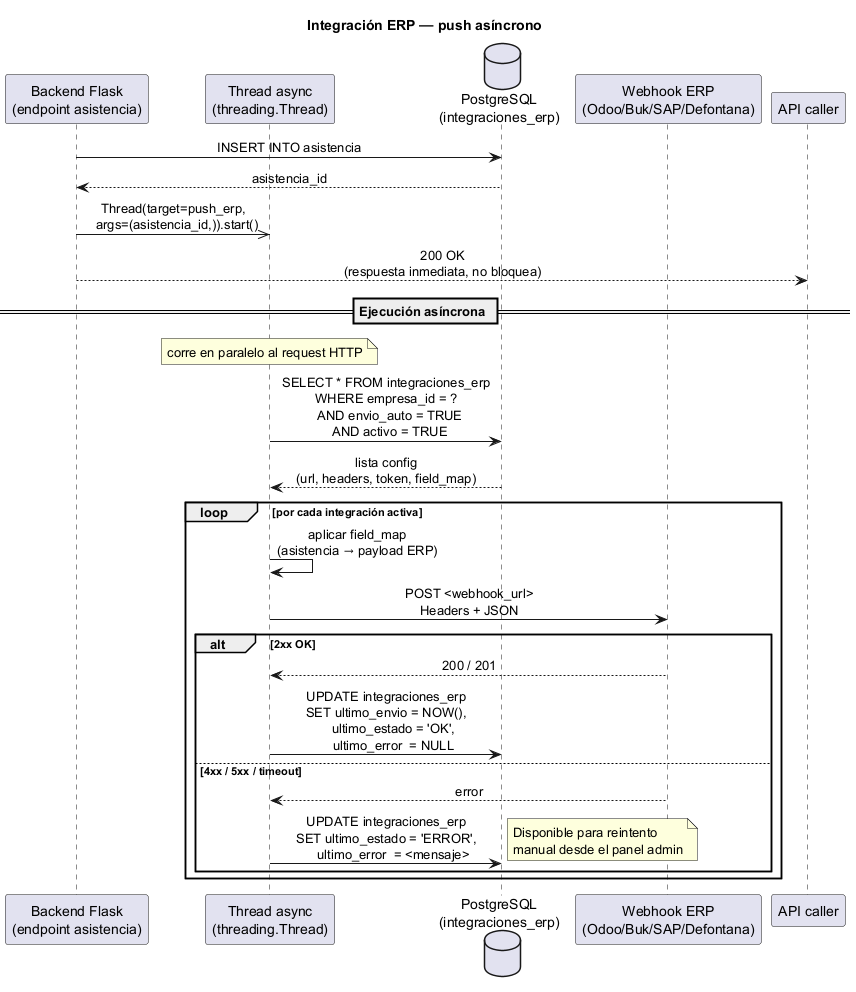
\includegraphics[width=0.95\linewidth]{diagrams/flujo_integracion_erp.png}
  \caption{Diagrama de secuencia de la integración ERP: push asíncrono con field mapping.}
  \label{fig:flujo_erp}
\end{figure}

\subsubsection{Implementación}

\paragraph{Panel web del backend}

Para complementar el backend, se desarrolló un panel web independiente (Next.js 16 \cite{nextjs_docs} con React 19 y TypeScript) cuyo módulo principal es la gestión del dispositivo IoT. Este panel, accesible desde cualquier navegador moderno, permite al administrador:

\begin{itemize}
    \item Visualizar el estado online/offline de cada dispositivo enrolado en tiempo real mediante tarjetas con código de colores, indicador animado (live-dot) y la IP como enlace clickable con la leyenda ``Misma red requerida''.
    \item Generar el PIN de 8 caracteres necesario para enrolar un nuevo ESP32-CAM.
    \item Probar la conectividad activa con un dispositivo específico consultando su endpoint /estado (variable NEXT\_PUBLIC\_DEVICE\_BASE\_URL, por defecto http://192.168.4.1).
    \item Renombrar y eliminar dispositivos registrados.
    \item Acceder a los logs de sincronización generados por el dispositivo.
    \item Acceder a las funcionalidades complementarias de gestión: personas, turnos, asignaciones, asistencias, integración ERP, usuarios y empresas.
\end{itemize}

El estado en tiempo real se obtiene mediante dos mecanismos complementarios. El principal es un hook useDeviceWebSocket que utiliza EventSource para conectarse directamente al endpoint SSE del backend (http://localhost:5000/sse/devices), recibiendo eventos con el id, nombre, IP, estado y timestamp del último heartbeat de cada dispositivo. Como respaldo, un temporizador ejecuta una consulta REST cada 15 segundos (GET /api/dispositivos) para actualizar el estado si la conexión SSE se interrumpe. El estado online se calcula verificando que el campo estado sea 'activo' y que el ultimo\_heartbeat esté dentro de los últimos 5 minutos; si alguna condición falla, el dispositivo se considera offline.

El panel web se comunica con el backend Flask mediante un proxy interno (app/api/\_proxy.ts) que reenvía las peticiones REST a la API, evitando problemas de CORS. La conexión SSE, por su parte, se realiza directamente al backend en el puerto 5000 sin pasar por el proxy, ya que requiere una conexión persistente text/event-stream. La aplicación está protegida por un middleware de autenticación que valida el token JWT y restringe el acceso según el rol del usuario (admin, empleador, trabajador). El frontend se compila con Docker en un build multi-etapa usando output: 'standalone' para producir una imagen optimizada lista para producción.

Para mantener la consistencia visual entre el panel web y la interfaz embebida del ESP32-CAM, las 9 vistas HTML del dispositivo (index.html, register.html, gestion.html, personas.html, turnos.html, asignaciones.html, asistencias.html, logs.html y wifi-setup.html) fueron actualizadas para adoptar la misma paleta oscura, tipografía y sistema de componentes del panel SAS. Se utilizaron variables CSS para la paleta cromática, diseño basado en tarjetas (cards) para la disposición del contenido, y componentes reutilizables para botones, tablas y formularios, logrando que ambas interfaces presenten una experiencia de usuario unificada.

Adicionalmente, el panel web incorpora las siguientes funcionalidades complementarias:

\begin{itemize}
    \item \textbf{Auto-registro de empresas}: La pantalla de inicio de sesión incluye un modo de registro que permite a nuevas empresas crear su cuenta directamente, invocando al endpoint público POST /api/auth/register-company. El formulario solicita nombre de la empresa y datos del administrador de la empresa (nombre, email, contraseña), y al enviarlo crea la organización, el usuario administrador y retorna un token JWT para acceso inmediato.
    \item \textbf{Captura facial por webcam}: El formulario de registro facial en el panel web utiliza la API navigator.mediaDevices.getUserMedia() para capturar fotografías directamente desde la cámara del navegador, eliminando la necesidad de subir archivos desde el sistema de archivos local. La interfaz permite visualizar la vista previa en vivo, capturar, previsualizar y confirmar o repetir la toma, con liberación adecuada del stream al cancelar.
    \item \textbf{Edición de usuarios del sistema}: Los administradores y empleadores pueden editar los datos de los usuarios del sistema (nombre, email, rol, contraseña, estado activo/inactivo) mediante un formulario modal que reutiliza la interfaz de registro en modo edición. Las actualizaciones son parciales: solo se envían los campos modificados.
\end{itemize}

\paragraph{Endpoint de configuración ERP para el ESP32-CAM}

Para que el ESP32-CAM pueda notificar asistencias directamente a los ERP configurados (incluso si el backend central no está disponible), se implementó el endpoint GET /api/dispositivos/erp-config, que retorna la lista de integraciones ERP activas con envío automático habilitado. El ESP32-CAM consulta este endpoint cada hora y almacena la configuración en /erp-config.json, permitiéndole enviar marcaciones a los ERP incluso durante desconexiones parciales.

\paragraph{Contraseñas para autenticación de dispositivos}

Para reforzar la seguridad en la comunicación entre el backend y los ESP32-CAM enrolados, se implementó un sistema de contraseñas de dispositivo que permite al administrador generar, gestionar y verificar credenciales específicas para cada terminal IoT. El flujo contempla cuatro operaciones:

\begin{itemize}
    \item \textbf{Generar contraseña} (POST /api/dispositivos/<id>/generar-password): El administrador solicita una nueva contraseña de 12 caracteres alfanuméricos, generada mediante secrets.choice(). El backend almacena el hash SHA256 de la contraseña, la versión en texto plano (temporal) y marca la contraseña como pendiente (password\_pendiente = TRUE). La respuesta incluye la contraseña en texto plano para que el administrador la proporcione al dispositivo.
    \item \textbf{Verificar contraseña pendiente} (GET /api/dispositivos/check-password): El ESP32-CAM, al iniciar, consulta este endpoint enviando su MAC address como header X-Device-MAC. Si hay una contraseña pendiente, el backend la retorna en texto plano para que el dispositivo la aplique localmente.
    \item \textbf{Confirmar contraseña} (POST /api/dispositivos/confirmar-password): Una vez que el dispositivo ha aplicado la contraseña localmente, confirma al backend, que limpia el texto plano (password\_plain = NULL) y desmarca el estado pendiente. A partir de este momento, solo el hash SHA256 permanece almacenado.
    \item \textbf{Eliminar contraseña} (DELETE /api/dispositivos/<id>/password): El administrador puede eliminar la contraseña de un dispositivo, limpiando el hash y el texto plano.
\end{itemize}

En el panel web, la sección de gestión de dispositivos incorpora botones para generar, regenerar y eliminar contraseñas, así como indicadores visuales del estado de la contraseña (tiene o no tiene, pendiente o confirmada).

\paragraph{Módulo de integración ERP}

El módulo routes/erp.py implementa:

\begin{itemize}
    \item \textbf{enviar\_asistencia\_a\_erps()}: Función central que itera sobre las integraciones ERP activas de una empresa, transforma los datos de la asistencia según el field mapping configurado, y envía una solicitud POST al webhook con los headers personalizados. Registra el resultado (ok o error) en la tabla integraciones\_erp (columnas ultimo\_envio y ultimo\_estado).

    \item \textbf{\_disparar\_erp\_push()}: Wrapper que ejecuta enviar\_asistencia\_a\_erps() en un hilo daemon separado, evitando que la latencia de los ERP externos afecte el tiempo de respuesta al ESP32-CAM. Esta función se invoca automáticamente desde create\_asistencia() y sync\_asistencias() cada vez que se registra una asistencia.

    \item \textbf{CRUD de integraciones}: Endpoints REST para crear, listar y eliminar configuraciones ERP.

    \item \textbf{Test de conectividad} (POST /api/erp/<id>/test): Envía un payload de prueba con datos ficticios al webhook configurado y retorna el código de respuesta y el cuerpo recibido.

    \item \textbf{Envío manual} (POST /api/erp/<id>/enviar): Envía las últimas 200 asistencias de la empresa al ERP seleccionado, útil para cargas históricas o reprocesamiento.

    \item \textbf{Estado de integración} (GET /api/erp/<id>/estado): Retorna el último envío y su estado.
\end{itemize}

\paragraph{Control remoto de dispositivos ESP32}

Se implementaron tres endpoints en routes/dispositivos.py que permiten controlar remotamente los ESP32-CAM enrolados mediante comandos MQTT:

\begin{itemize}
    \item \textbf{Registrar huella} (POST /api/dispositivos/<id>/registrar-huella): Recibe un persona\_id y envía al dispositivo el comando para iniciar el enrolamiento de una huella digital. Verifica que el dispositivo exista, que pertenezca a la empresa del usuario autenticado, y que la persona exista en la misma empresa. Utiliza enviar\_comando\_dispositivo(mac, 'registrar\_huella') para publicar el comando en backend/comando/<MAC>/registrar\_huella. El resultado del enrolamiento se recibe luego por el tópico esp32/huella/resultado/\#.

    \item \textbf{Reiniciar dispositivo} (POST /api/dispositivos/<id>/reiniciar): Envía el comando reiniciar al ESP32-CAM, provocando un reinicio remoto del dispositivo. Útil para recuperar un dispositivo que presenta fallos de conectividad o para aplicar cambios de configuración. Si el cliente MQTT no está disponible, retorna HTTP 503.

    \item \textbf{Reconectar Wi-Fi} (POST /api/dispositivos/<id>/wifi-reconnect): Envía el comando wifi-reconnect para que el dispositivo reinicie su conexión Wi-Fi. Permite recuperar un dispositivo que ha perdido la conectividad sin necesidad de intervención física.
\end{itemize}

Los tres endpoints están protegidos con \textbf{"@requiere\_rol('admin', 'empleador')"} y verifican que el dispositivo pertenezca a la empresa del usuario autenticado. Los comandos se publican en el tópico backend/comando/<MAC>/<comando> mediante la función enviar\_comando\_dispositivo() del módulo mqtt\_handler.py.

\subsubsection{Pruebas}

Se diseñaron las siguientes pruebas para validar el panel web para la gestión del dispositivo y la integración ERP:

\begin{itemize}
    \item \textbf{Prueba de streaming SSE}: Conectar el navegador a http://localhost:5000/sse/devices y verificar que se reciban eventos text/event-stream con datos JSON de los dispositivos. Simular un heartbeat desde un ESP32-CAM y verificar que el evento SSE refleje el cambio a estado activo. Desconectar el dispositivo y verificar que el evento SSE refleje el estado inactivo.

    \item \textbf{Prueba de fallback polling}: Interrumpir la conexión SSE (deteniendo el servidor backend momentáneamente). Verificar que el panel web continúe mostrando el estado de los dispositivos mediante las consultas REST periódicas (cada 15 segundos) y que al restaurar la conexión SSE se retome el streaming.

    \item \textbf{Prueba de indicador visual de dispositivo}: Verificar que cada tarjeta de dispositivo en el panel web muestre: la dirección IP como enlace clickable que abre http://<ip>/ en una nueva pestaña, un indicador animado verde/rojo (live-dot) que refleje el estado online/offline, y la leyenda ``Misma red requerida'' como sugerencia contextual.

    \item \textbf{Prueba de navegación en panel web}: Acceder a las rutas principales del backend (/health, /api/personas, /api/asistencias) sin autenticación y verificar que respondan correctamente (HTTP 200 con acceso público o HTTP 401 cuando se requiera token).

    \item \textbf{Prueba de creación de integración ERP}: Autenticarse como empleador y enviar POST /api/erp con nombre, tipo, webhook URL (usando un servidor de prueba como https://webhook.site) y field mapping. Verificar que la integración se cree con activo = TRUE y envio\_auto = TRUE.

    \item \textbf{Prueba de test de webhook}: Ejecutar POST /api/erp/<id>/test para la integración creada. Verificar que el webhook de prueba reciba un payload JSON con datos ficticios (rut = '11.111.111-1', nombre = "Test Usuario", tipo = "entrada"). Verificar que el estado se actualice en la base de datos.

    \item \textbf{Prueba de envío automático}: Registrar una asistencia real (POST a /api/asistencias) para una persona de la empresa configurada. Verificar que el servidor de prueba del webhook reciba automáticamente el payload con los datos de la asistencia.

    \item \textbf{Prueba de field mapping}: Configurar un ERP con field mapping \{"rut": "employee\_id", "tipo": "event"\}. Registrar una asistencia y verificar que el webhook reciba el payload con los campos renombrados (employee\_id en lugar de rut, event en lugar de tipo).

    \item \textbf{Prueba de envío asíncrono}: Medir el tiempo de respuesta del endpoint POST /api/asistencias cuando hay un ERP configurado cuyo webhook tarda 5 segundos en responder. Verificar que la respuesta al cliente sea inmediata (menor a 200 ms) y que el envío al ERP ocurra en segundo plano.

    \item \textbf{Prueba de tolerancia a fallos ERP}: Configurar un webhook que retorne HTTP 500. Registrar una asistencia y verificar que el sistema no falle; el error debe quedar registrado en ultimo\_estado de la integración y la asistencia debe persistirse correctamente en la base de datos.

    \item \textbf{Prueba de sincronización de configuración ERP al ESP32-CAM}: Simular la consulta GET /api/dispositivos/erp-config desde el ESP32-CAM (con header X-Device-MAC). Verificar que retorne solo las integraciones activas con envío automático de la empresa correspondiente.

    \item \textbf{Prueba de envío manual por lote}: Ejecutar POST /api/erp/<id>/enviar y verificar que se envíen correctamente los registros de asistencia recientes al webhook del ERP.
\end{itemize}

\subsubsection{Refinamientos posteriores}

\begin{itemize}
    \item \textbf{Reasignación de dispositivos entre empresas}: se agregó el endpoint PUT /api/dispositivos/<id>/reasignar, restringido al rol admin, que permite mover un dispositivo ya enrolado de una empresa a otra actualizando su columna empresa\_id. Esto resuelve el caso de dispositivos físicos que cambian de destino (por ejemplo, al reasignar hardware entre sucursales o clientes) sin requerir un nuevo proceso de enrolamiento con PIN.

    \item \textbf{Zona horaria de Chile en la integración ERP}: los timestamps enviados a los webhooks ERP se normalizan a America/Santiago mediante el módulo estándar zoneinfo, con conversión explícita antes de formatear cada fecha\_hora y timestamp del payload. Esto evita ambigüedades cuando el servidor del backend opera en UTC y el sistema ERP de destino espera horarios locales.

    \item \textbf{Soporte de múltiples fotos en el panel web}: el panel de administración construido con Next.js incorpora en la vista de cada persona la visualización de las fotos de referencia asociadas a sus distintos encodings\_faciales, reflejando en la interfaz la capacidad de multi-encoding ya descrita en la Sección 2.3.10. Asimismo, en los despliegues multi-empresa la interfaz incorpora una indicación visual de la empresa a la que pertenece cada registro, relevante para el rol admin, que puede ver datos de más de una organización.
\end{itemize}


%% ============================================================
%% ITERACIÓN 8: Sincronización diferida, logs y cierre del proyecto
%% ============================================================

\subsection{Iteración 8: Sincronización diferida, logs y cierre del proyecto}

Esta iteración integra la sincronización diferida entre el ESP32-CAM y el backend, la capa de auditoría y logs del sistema, y las herramientas de diagnóstico.

\subsubsection{Análisis}

Para que el prototipo sea viable en entornos reales, debe garantizar que ningún dato se pierda durante períodos de desconexión y que todas las operaciones críticas queden registradas para auditoría. Los requisitos identificados son:

\begin{itemize}
    \item \textbf{Sincronización diferida de asistencias}: Los registros de asistencia generados offline (marcados con sincronizado = false) deben enviarse automáticamente al backend cuando se restablezca la conectividad. El proceso debe ser idempotente: si un registro ya existe en el backend, no debe duplicarse.
    \item \textbf{Sincronización diferida de entidades}: Las personas, turnos y asignaciones creados localmente durante el modo offline deben sincronizarse con el backend, resolviendo conflictos de identificadores (IDs locales con prefijo local- versus IDs del backend).
    \item \textbf{Sincronización de configuración ERP}: La configuración de integraciones ERP debe poder descargarse desde el backend para que el ESP32-CAM pueda enviar datos de asistencia directamente a los ERP configurados.
    \item \textbf{Logs de sincronización}: Cada operación de sincronización debe registrarse en la base de datos con el conteo de registros enviados y procesados correctamente, permitiendo auditoría posterior.
    \item \textbf{Logs biométricos}: Todas las operaciones de registro, verificación e identificación facial deben quedar registradas con timestamp, resultado e IP de origen, para cumplimiento normativo.
    \item \textbf{Watchdog de dispositivos}: El backend debe monitorear continuamente el estado de los dispositivos enrolados, detectando aquellos que han dejado de comunicarse y marcándolos como inactivos.
    \item \textbf{Herramientas de diagnóstico}: Se requiere un script de prueba que permita simular asistencias faciales usando fotos almacenadas, facilitando las pruebas del sistema sin necesidad del hardware.
\end{itemize}

\subsubsection{Diseño}

\paragraph{Proceso de sincronización diferida}

El ESP32-CAM ejecuta la sincronización en dos momentos:
\begin{enumerate}
    \item \textbf{Al iniciar}: Si hay conectividad, llama a sincronizarPendientes() que ejecuta en secuencia:
    \begin{itemize}
        \item sincronizarTurnosPendientes(): Envía los turnos con sincronizado = false al backend vía POST, y actualiza sus backend\_id.
        \item sincronizarAsignacionesPendientes(): Similar para asignaciones, dependiendo de que los turnos referenciados ya tengan backend\_id.
        \item sincronizarAsistencias(): Envía un lote de asistencias con sincronizado = false vía POST /api/asistencias/sync.
    \end{itemize}
    \item \textbf{Periódicamente}: Cada 5 minutos (300,000 ms), se ejecuta sincronizarPendientes() en el bucle principal.
\end{enumerate}

Además, el ESP32-CAM consulta GET /api/dispositivos/erp-config cada hora (360,000 ms) para mantener actualizada su configuración local de webhooks ERP.

\begin{figure}[H]
  \centering
  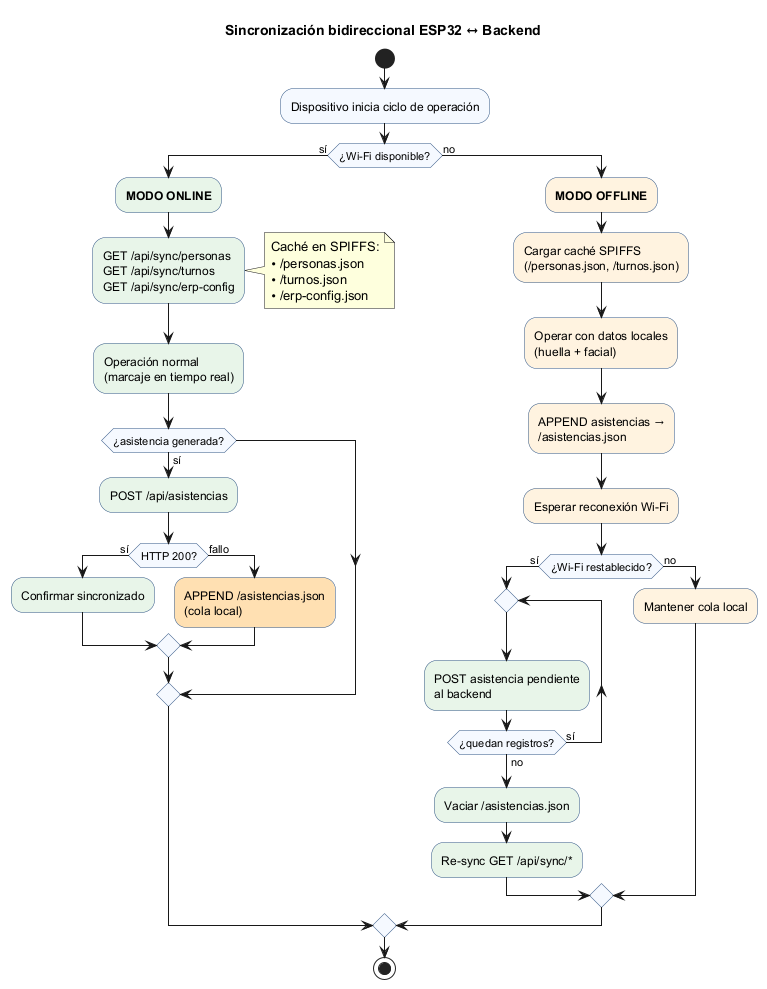
\includegraphics[width=0.95\linewidth]{diagrams/flujo_sincronizacion_bidireccional.png}
  \caption{Diagrama de actividad: sincronización bidireccional entre los modos online y offline del ESP32-CAM.}
  \label{fig:flujo_sync}
\end{figure}

\paragraph{Deduplicación en el backend}

El endpoint POST /api/asistencias/sync implementa una verificación previa a la inserción: para cada registro del lote, consulta si ya existe una asistencia de la misma persona (persona\_id), mismo tipo (entrada/salida), mismo turno\_id y misma fecha (DATE(fecha\_hora) = CURRENT\_DATE). Si existe, omite la inserción. Esta verificación por turno\_id permite que un trabajador registre múltiples asistencias en un mismo día si pertenece a distintos turnos (por ejemplo, jornada diurna y jornada nocturna), sin generar duplicados dentro del mismo turno. Garantiza idempotencia ante reenvíos.

\paragraph{Tablas de auditoría}

\begin{itemize}
    \item sincronizacion\_log: Registra cada operación de sincronización con: dispositivo de origen, cantidad de registros enviados, cantidad procesada correctamente, estado y detalle.
    \item logs\_biometricos: Registra cada operación biométrica con: persona, dispositivo, timestamp, tipo de operación (registro, verificación, identificación), resultado (éxito, fallo, duplicado, no\_encontrado) e IP de origen.
    \item eliminaciones\_biometricas: Registra cada eliminación de datos biométricos con: persona, embedding anterior (cifrado), ruta de la foto eliminada y usuario solicitante.
\end{itemize}

\paragraph{Panel de visualización de logs}

El backend expone dos conjuntos de endpoints para consulta de logs:
\begin{itemize}
    \item GET /api/logs: Lista los registros de sincronización, con filtro por empresa para roles no-admin.
    \item DELETE /api/logs: Permite limpiar los logs (admin limpia todo, empleador limpia los de su empresa).
    \item El ESP32-CAM expone GET /api/logs que retorna el buffer de logs en formato HTML, y /api/logs/clear para limpiarlo.
\end{itemize}

\paragraph{Script de simulación de asistencia facial}

Se desarrolló deteccion.py, un script de línea de comandos que permite probar el flujo de reconocimiento facial sin necesidad del ESP32-CAM. El script escanea las fotos almacenadas localmente para el ambiente de pruebas, presenta un menú interactivo para seleccionar una de ellas, ejecuta el proceso de identificación 1:N contra la base de datos y registra la asistencia correspondiente. Es útil para pruebas de regresión rápida y demostraciones.

\subsubsection{Implementación}

\paragraph{Sincronización en el ESP32-CAM}

Las funciones de sincronización siguen un patrón común:

\begin{enumerate}
    \item Verificar conectividad (isOnline y WiFi.status() == WL\_CONNECTED).
    \item Cargar los datos locales desde LittleFS.
    \item Iterar sobre los registros con sincronizado = false.
    \item Para cada uno, construir el payload JSON y enviarlo al backend vía HTTP POST.
    \item Si el backend responde con éxito (HTTP 200/201), marcar sincronizado = true y actualizar el backend\_id si corresponde.
    \item Persistir los cambios en LittleFS.
\end{enumerate}

Para las personas, además del envío de pendientes, se implementa la descarga completa desde el backend (sincronizarPersonasDesdeBackend()) que sobrescribe el archivo local si no hay registros locales pendientes, manteniendo el ESP32-CAM actualizado con los datos del servidor.

\paragraph{Campo colación en turnos}

Los turnos incorporaron los campos con\_colacion (booleano), colacion\_inicio (TIME) y colacion\_fin (TIME) para modelar el horario de colación de los trabajadores, en cumplimiento del artículo 34 del Código del Trabajo chileno. En la tabla turnos de PostgreSQL se almacenan como TIME (o NULL si con\_colacion = FALSE). Los endpoints CRUD de routes/turnos.py gestionan estos campos: al crear un turno, se envían con\_colacion, colacion\_inicio y colacion\_fin; al actualizar, se usa COALESCE para preservar valores existentes si no se envían. Las consultas GET retornan los horarios como string o null según corresponda. El campo turno\_id se agregó también a la tabla asistencias para asociar cada marcación al turno bajo el cual se registró, permitiendo el cálculo preciso de horas trabajadas descontando la colación.

\paragraph{Sincronización de asistencias por lote}

La función sincronizarAsistencias() en el ESP32-CAM es especialmente relevante porque maneja el caso más frecuente de datos offline: un trabajador marcó entrada y salida durante el día sin conexión. La función:

\begin{enumerate}
    \item Carga asistencias.json y filtra las que tengan sincronizado = false.
    \item Construye un JSON con estructura \{"registros": [...]\}.
    \item Lo envía a POST /api/asistencias/sync.
    \item Si el backend retorna HTTP 200, marca todos los registros enviados como sincronizados.
\end{enumerate}

\paragraph{Sincronización en el backend}

El endpoint POST /api/asistencias/sync en routes/asistencias.py recibe el lote e itera sobre cada registro, aplicando la verificación de duplicados y realizando la inserción. También dispara el envío a ERP para cada asistencia nueva.

\paragraph{Watchdog y ping activo de dispositivos}

La detección de desconexión de dispositivos se implementó con tres capas complementarias:

\begin{enumerate}
    \item \textbf{LWT (instantáneo)}: Al conectarse al broker MQTT, el ESP32-CAM configura un mensaje Last Will en esp32/lwt/<MAC>. Si el dispositivo se desconecta abruptamente, el broker publica automáticamente el LWT y el backend marca el dispositivo como inactivo de inmediato.
    \item \textbf{Ping activo (device\_pinger)}: Un hilo separado publica periódicamente (cada 30 segundos) un mensaje en el tópico esp32/ping/<MAC>. El ESP32-CAM, al recibirlo, responde publicando un heartbeat con el campo "pong": true. Si el backend no recibe respuesta dentro de 60 segundos, marca el dispositivo como inactivo. Este mecanismo funciona incluso si el mensaje LWT no fue entregado.
    \item \textbf{Watchdog pasivo (device\_watchdog)}: Un hilo ejecutado cada 60 segundos realiza un barrido inicial al arrancar el backend (todos los dispositivos se marcan inactivo) y luego verifica periódicamente qué dispositivos no han enviado heartbeat en más de 90 segundos, marcándolos como inactivos.
\end{enumerate}

Esta arquitectura de tres capas asegura que ninguna desconexión pase desapercibida: el LWT atrapa las desconexiones abruptas detectadas por el broker; el ping activo detecta silencios de red donde el LWT no alcanza a publicarse; y el watchdog pasivo actúa como respaldo final para cualquier caso no cubierto por las capas anteriores.

\paragraph{Herramienta de simulación facial}

Como complemento durante el desarrollo se implementó deteccion.py, un script de línea de comandos que permitió probar el flujo de reconocimiento facial sin necesidad del ESP32-CAM. El script se conectaba directamente a PostgreSQL, ejecutaba DeepFace (Facenet + detector configurable + anti-spoofing) sobre imágenes almacenadas localmente para el ambiente de pruebas, y registraba asistencias de prueba en la base de datos. En las etapas finales del proyecto, esta funcionalidad de simulación fue absorbida por la suite de pruebas automatizadas (con mocks de DeepFace, OpenCV y PostgreSQL en Docker), que ofrece mayor repetibilidad y cobertura sin dependencia del sistema de archivos local.

\paragraph{Flujo operacional consolidado}
\label{sec:flujo_operacional_consolidado}

Con todos los componentes del sistema ya construidos (enrolamiento por PIN, reconocimiento biométrico, almacenamiento offline, sincronización diferida e integración ERP), la Fig.~\ref{fig:flujo_operacional} consolida el camino completo que sigue una marcación, cubriendo tanto el caso con conexión a internet como el caso sin ella, tal como quedó implementado al cierre del proyecto.

El flujo comienza cuando el sensor PIR detecta presencia frente al dispositivo y se ejecuta la captura biométrica (huella mediante el AS608 o rostro mediante la cámara OV2640). A partir de ahí, el firmware evalúa isCloudReady(): si el dispositivo está conectado a internet y enrolado, la marcación se envía de inmediato al backend por HTTP (POST /api/facial/identificar para rostro, o POST /api/asistencias para huella). Si cualquiera de esas dos condiciones falla, la marcación se guarda localmente en asistencias.json (LittleFS) con la marca sincronizado=false, se muestra el resultado en el panel embebido sin esperar respuesta del servidor, y el dispositivo queda a la espera de que la conexión se restablezca para ejecutar sincronizarPendientes(), que vacía la cola completa hacia el backend.

Ambos caminos, el envío inmediato y la sincronización diferida, terminan convergiendo en el mismo punto: el backend valida la huella o el rostro contra los registros almacenados (encodings\_faciales o el identificador de huella) y persiste el resultado en la tabla asistencias de PostgreSQL. Si la identificación es exitosa, el backend responde 200 OK, dispara en un hilo aparte el envío hacia los sistemas ERP configurados, y el firmware ejecuta flashExito(), que hace parpadear el LED verde del dispositivo dos veces. Si no hay coincidencia o la imagen no cumple el filtro de calidad, el backend responde con un código de error (404 o 400) y la operación queda registrada en logs\_biometricos para su auditoría posterior; en este caso el firmware invoca flashError(), una función que existe en el código como punto de extensión para una señal de error distinta, pero que actualmente no tiene ninguna acción implementada.

\begin{figure}[H]
    \centering
    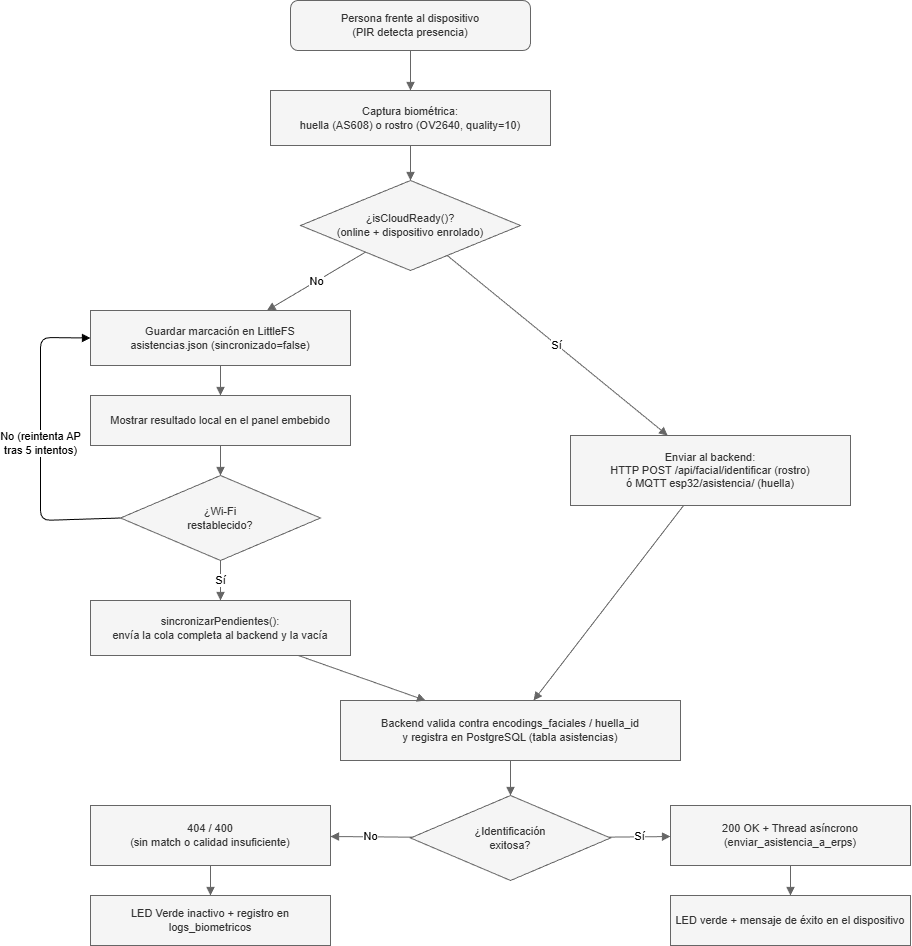
\includegraphics[width=.85\linewidth]{Imagenes/flujo_operacional_asistencia.png}
    \caption{Flujo operacional consolidado para el registro de asistencia.}
    \label{fig:flujo_operacional}
\end{figure}

\subsubsection{Pruebas}
\label{sec:pruebas_unitarias_automatizadas}

Se diseñaron las siguientes pruebas para validar la sincronización diferida, los logs y la integración final:

\begin{itemize}
    \item \textbf{Prueba de sincronización de asistencias offline}: Desconectar el ESP32-CAM de la red, registrar 5 marcaciones de entrada/salida para 2 personas diferentes, reconectar y ejecutar sincronización. Verificar que los 5 registros aparezcan en la base de datos del backend y que el archivo asistencias.json local los marque como sincronizados.

    \item \textbf{Prueba de idempotencia de sincronización}: Tras una sincronización exitosa, ejecutar nuevamente la sincronización sin nuevos registros. Verificar que no se inserten registros duplicados en el backend.

    \item \textbf{Prueba de sincronización de personas creadas offline}: Desconectar el dispositivo, registrar una nueva persona (con huella y datos), reconectar y sincronizar. Verificar que la persona aparezca en el backend con un ID definitivo (no local-).

    \item \textbf{Prueba de sincronización de turnos y asignaciones}: Desconectar el dispositivo, crear un turno y asignarlo a una persona existente, reconectar y sincronizar. Verificar que el turno y la asignación se repliquen en el backend y que los backend\_id locales se actualicen correctamente.

    \item \textbf{Prueba de persistencia tras corte de energía}: Durante una sincronización en curso, cortar la alimentación del ESP32-CAM. Al reiniciar, verificar que los archivos JSON no estén corruptos y que los registros con sincronizado = false sigan estando disponibles para una nueva sincronización.

    \item \textbf{Prueba de duplicados por turno}: Registrar dos asistencias con la misma persona, tipo, turno y fecha. Verificar que el sistema rechace la segunda inserción por duplicado. Registrar asistencias con diferentes turno\_id para un mismo día y verificar que ambas se registren sin conflictos.

    \item \textbf{Prueba de colación en turnos}: Crear un turno con colación habilitada (con\_colación = true) especificando horario de colación. Verificar que los campos colacion\_inicio y colacion\_fin se almacenen correctamente como TIME en la base de datos. Crear un turno sin colación y verificar que ambos campos sean NULL.

    \item \textbf{Prueba de logs de sincronización}: Ejecutar 3 sincronizaciones con diferentes cantidades de registros. Verificar que en la tabla sincronizacion\_log del backend aparezcan 3 entradas con los conteos correctos de registros enviados y procesados.

    \item \textbf{Prueba de logs biométricos}: Realizar operaciones de registro facial, identificación exitosa, identificación fallida y verificación. Verificar que cada operación genere una entrada en logs\_biometricos con el tipo de operación y resultado correctos.

    \item \textbf{Prueba de watchdog}: Iniciar el backend, verificar que todos los dispositivos se marquen como inactivos. Conectar un ESP32-CAM, verificar que tras el primer heartbeat cambie a activo. Desconectar el ESP32-CAM y verificar que tras 90 segundos el watchdog lo marque como inactivo.

    \item \textbf{Prueba de ping activo}: Conectar un ESP32-CAM, verificar que el backend publique pings en esp32/ping/<MAC> y que el dispositivo responda. Detener el ESP32-CAM (corte de red) y verificar que el ping activo marque el dispositivo como inactivo antes de que el watchdog de 90 segundos actúe (tiempo de espera de 60 segundos).

    \item \textbf{Prueba de simulación facial automatizada}: Utilizar la suite de pruebas test\_routes\_facial.py y el emulador test\_identificacion\_facial.py para simular el flujo completo de identificación 1:N con imágenes sintéticas generadas en memoria, cubriendo casos de coincidencia exitosa, rostro no registrado y calidad insuficiente de imagen.

    \item \textbf{Prueba de flujo completo punta a punta}: Ejecutar el flujo completo: registrar persona con huella y rostro en el ESP32-CAM $\rightarrow$ sincronizar con backend $\rightarrow$ verificar que la persona aparezca en el panel web $\rightarrow$ marcar asistencia por huella offline $\rightarrow$ reconectar y sincronizar $\rightarrow$ verificar que la asistencia aparezca en el panel web y se envíe al ERP de prueba.
\end{itemize}

\paragraph{Pruebas automatizadas}

Además de las pruebas funcionales descritas, se implementó una suite de más de 590 pruebas automatizadas para el backend y el firmware, utilizando pytest con PostgreSQL en Docker y mocks para DeepFace, OpenCV y MQTT. La suite se organiza en 35 archivos de prueba y alcanza una cobertura de código del 98\% sobre el código de producción del backend, sin fallos en ninguna de las pruebas (ver Anexo D para el detalle de casos y la evolución de la cobertura por módulo). La integración con los ERP externos se valida en dos niveles: por un lado, las pruebas de la suite automatizada cubren la creación, edición y prueba de webhooks de una integración ERP, simulando la respuesta del servidor externo. Por otro lado, dentro del subdirectorio ERPSIMULATORS/ se construyeron tres simuladores independientes (mock\_odoo.py, mock\_defontana.py y mock\_buk.py), cada uno levantando un pequeño servidor Flask que reproduce los endpoints reales de autenticación, consulta de empleados e inyección de marcaciones de su respectivo ERP comercial, según la documentación pública de cada proveedor. El script test\_erp\_mocks.py se ejecuta por separado, con los tres simuladores corriendo: envía una marcación con el formato que genera el sistema hacia cada uno de los tres mocks y verifica que el field mapping configurado para cada ERP transforme correctamente los datos y que cada simulador responda como lo haría el sistema real, imprimiendo un reporte de éxito o falla por caso. Esta validación manual complementa, sin sustituir, a las pruebas automatizadas de pytest.

Las pruebas cubren los flujos de todas las iteraciones: inicialización de la aplicación, esquema de base de datos, cifrado de embeddings, servicio de correo electrónico (con mock de SMTP), handlers MQTT, autenticación JWT con roles jerárquicos y flujo multi-empresa, endpoints faciales, CRUD de personas/turnos/asignaciones/asistencias, verificación de dispositivos, integraciones ERP con tolerancia a fallos de conexión y timeout, enrolamiento de dispositivos mediante PIN, sincronización offline, y logs de auditoría. Entre los módulos con mayor cobertura destacan el cifrado de embeddings (100\%), el servicio de correo (100\%), la gestión de turnos (100\%), la base de datos (99\%) y el módulo de asignaciones (96\%). El detalle completo de los casos de prueba se incluye en el Anexo D, que además resume los resultados obtenidos al ejecutar la suite completa.

\subsubsection{Refinamientos posteriores}

\begin{itemize}
    \item \textbf{Limpieza de datos al eliminar una persona}: el endpoint de eliminación distingue dos comportamientos según el rol de quien lo invoca. Un administrador ejecuta una limpieza completa de datos biométricos y sensibles: anonimiza el RUT, el correo y el identificador de huella, elimina los encodings\_faciales y los consentimientos asociados, borra la foto de previsualización del disco y marca a la persona como inactiva, conservando únicamente su historial de asistencias. Un empleador, en cambio, solo puede marcar a la persona como inactiva, sin acceso a la limpieza de datos biométricos, reservada al rol con mayor privilegio.

    \item \textbf{Filtro activo = true en los listados}: todas las consultas de lectura sobre personas (y entidades equivalentes) incorporan la condición WHERE activo = true, de modo que los registros eliminados mediante soft-delete dejan de aparecer en listados y búsquedas sin perder su información histórica en la base de datos, requisito necesario para mantener la integridad de los reportes de asistencia ya generados.
\end{itemize}


\section{Mecanismos de seguridad}

Esta sección consolida los mecanismos de seguridad implementados a lo largo de las distintas iteraciones, descritos en su momento dentro del desarrollo de cada una (Secciones 4.2.3 a 4.2.5), agrupándolos por capa: autenticación y control de acceso, enrolamiento de dispositivos, y protección de datos biométricos.

\subsection{Autenticación y control de acceso}

El backend define tres decoradores de autenticación en routes/auth.py, aplicados según el tipo de cliente que consume cada endpoint:

\begin{itemize}
    \item @token\_required: exige un header Authorization: Bearer <token> con un JWT firmado con el algoritmo HS256 y una clave secreta (JWT\_SECRET, configurable por variable de entorno). El token incluye user\_id, empresa\_id, rol y, opcionalmente, persona\_id, con una expiración de 24 horas. Si el token falta, está expirado o es inválido, el endpoint responde con HTTP 401.

    \item @requiere\_rol(*roles): envuelve a @token\_required y además exige que request.user\_rol esté dentro de los roles permitidos (admin, empleador o trabajador), respondiendo HTTP 403 en caso contrario. Implementa así un control de acceso jerárquico basado en roles sobre los mismos endpoints autenticados.

    \item @token\_opcional: permite que un mismo endpoint sea consumido tanto por un cliente web autenticado con JWT como por un dispositivo ESP32-CAM identificado mediante el header X-Device-MAC. Si no hay JWT, el decorador busca la MAC recibida entre los dispositivos ya enrolados y, de encontrarla, expone request.dispositivo\_id y request.empresa\_id para el resto del endpoint. Como se detalla en la Sección 4.2.5, este decorador ya no crea dispositivos nuevos automáticamente: solo vincula los que ya pasaron por el flujo de enrolamiento con PIN.

    \item @requiere\_dispositivo\_enrolado: complementa a @token\_opcional en endpoints biométricos sensibles (por ejemplo, /api/facial/registrar), verificando explícitamente que el dispositivo de la petición tenga enrolado = TRUE en la base de datos antes de continuar, y respondiendo HTTP 403 en caso contrario.
\end{itemize}

Las contraseñas de los usuarios del panel web nunca se almacenan en texto plano: se procesan con bcrypt \cite{bcrypt_pypi} (función hashpw con sal generada por gensalt()) tanto al crear una cuenta como al cambiar la contraseña, y la verificación en el login usa bcrypt.checkpw para comparar contra el hash almacenado.

\subsection{Enrolamiento seguro de dispositivos}

Un dispositivo ESP32-CAM no puede operar contra el backend simplemente conectándose a la red: debe pasar por un flujo de enrolamiento explícito basado en un PIN de un solo uso. Un administrador o empleador solicita POST /api/auth/dispositivos/generar-pin, que crea en la base de datos un registro en dispositivos con enrolado = FALSE y un código aleatorio de 8 caracteres alfanuméricos (generado con el módulo secrets, criptográficamente seguro). El dispositivo, desde su panel de configuración Wi-Fi, envía ese PIN junto con su dirección MAC al backend; si el PIN es válido y no fue usado antes, el dispositivo queda marcado como enrolado = TRUE y asociado a la MAC y a la empresa que generó el PIN. Un PIN ya consumido no puede reutilizarse (HTTP 409).

En el firmware, la función isCloudReady() (Sección 4.2.1) actúa como una verificación de doble factor antes de cualquier operación dependiente del backend: exige tanto conectividad de red (isOnline) como enrolamiento confirmado (estaEnrolado), evitando que un dispositivo conectado pero no autorizado, o autorizado pero sin red, ejecute operaciones que comprometerían la consistencia del sistema.

\subsection{Protección de datos biométricos}

Los embeddings faciales generados por DeepFace se cifran antes de almacenarse en la base de datos mediante Fernet (AES-128 en modo CBC con autenticación HMAC-SHA256), de la librería cryptography de Python. La clave de cifrado no se almacena directamente: se deriva aplicando SHA-256 a una variable de entorno (BIOMETRIC\_KEY) y codificando el resultado en base64 URL-safe, tal como lo exige la API de Fernet:

\begin{verbatim}
def _derivar_fernet_key() -> bytes:
    digest = hashlib.sha256(BIOMETRIC_KEY.encode("utf-8")).digest()
    return base64.urlsafe_b64encode(digest)
\end{verbatim}

De esta forma, ni el embedding ni la clave de cifrado quedan expuestos en texto plano en la base de datos: un acceso no autorizado a las tablas encodings\_faciales solo expone valores cifrados, mientras la clave reside exclusivamente en la configuración del entorno de ejecución del backend.

\section{Arquitectura de tiempo real (SSE)}

El panel web necesita reflejar, sin recargar la página, el estado de conexión de cada ESP32-CAM y el progreso del enrolamiento de huellas. Esta sección consolida cómo se implementó esa capa de tiempo real, descrita parcialmente al introducirse en las iteraciones 3 y 7 (Secciones 4.2.3 y 4.2.5).

\subsection{Endpoints de streaming}

El backend expone dos endpoints SSE (Server-Sent Events) implementados en app.py con el patrón estándar de Flask para streaming: una función generadora que produce eventos en formato text/event-stream, devuelta mediante Response(stream\_with\_context(generate()), mimetype='text/event-stream').

\begin{itemize}
    \item GET /sse/devices: difunde, a todos los clientes conectados, los cambios de estado de los dispositivos (heartbeat recibido, LWT disparado, ping sin respuesta), mediante la función broadcast\_device\_update().
    \item GET /sse/huellas: difunde el resultado del enrolamiento de huellas recibido por MQTT en esp32/huella/resultado/\#, mediante broadcast\_huella\_update(), permitiendo que el panel muestre en vivo el progreso del registro biométrico.
\end{itemize}

Se optó por SSE porque el caso de uso es unidireccional (servidor a cliente) y se consume en el navegador con la API nativa EventSource, sin depender de librerías adicionales en el frontend ni de un protocolo de negociación propio como el de WebSockets.

\subsection{Tres capas de detección de desconexión}

Determinar si un ESP32-CAM sigue conectado es más complejo que solo esperar sus heartbeats, porque una caída de red puede impedir que el dispositivo avise que se desconectó. El backend combina tres mecanismos complementarios, implementados en mqtt\_handler.py:

\begin{enumerate}
    \item \textbf{LWT (Last Will and Testament)}: al conectarse al broker MQTT, el ESP32-CAM registra un mensaje LWT en esp32/lwt/<MAC>. Si la conexión TCP se rompe de forma anómala (corte de energía, pérdida abrupta de señal), el propio broker Mosquitto publica ese mensaje automáticamente, sin que el backend tenga que esperar ningún timeout. Es la capa más rápida, pero depende de que el broker detecte la caída de la conexión subyacente.

    \item \textbf{Ping activo (device\_pinger)}: un hilo en segundo plano publica, cada 30 segundos, un mensaje en esp32/ping/<MAC> para cada dispositivo enrolado. El ESP32-CAM responde con un heartbeat normal al recibirlo. Si un dispositivo no responde dentro de la ventana definida por HEARTBEAT\_TIMEOUT (60 segundos), el pinger lo marca como inactivo directamente, sin esperar al watchdog. Esta capa cubre los casos en que el LWT no llega a publicarse (por ejemplo, si el broker tampoco detecta la caída).

    \item \textbf{Watchdog pasivo (device\_watchdog)}: un segundo hilo revisa cada 60 segundos la antigüedad del último heartbeat de cada dispositivo y marca como inactivos a los que superan los 60 segundos sin responder. Actúa como respaldo final, independiente del pinger, y además ejecuta un barrido inicial al arrancar el backend que marca a todos los dispositivos como inactivos hasta recibir su primer heartbeat.
\end{enumerate}

Cada vez que cualquiera de estas tres capas cambia el estado de un dispositivo en la base de datos, invoca broadcast\_device\_update(), que propaga el cambio de inmediato a los clientes SSE conectados.

\subsection{Consumo en el frontend}

En el panel web (Next.js), un hook personalizado se conecta directamente al endpoint /sse/devices mediante EventSource, actualizando en memoria el estado, IP y último heartbeat de cada dispositivo a medida que llegan eventos, sin necesidad de refrescar la página ni de mantener una conexión WebSocket. Como mecanismo de respaldo ante una eventual interrupción de la conexión SSE, el frontend además consulta periódicamente GET /api/dispositivos por REST, de modo que el estado mostrado no depende exclusivamente del canal de streaming.

\section{Prototipo final}
\label{sec:prototipo_final}

Esta sección presenta el resultado físico del proceso de desarrollo descrito en las ocho iteraciones anteriores, mostrando el dispositivo ESP32-CAM ensamblado junto con sus componentes periféricos (cámara OV2640, lector de huellas AS608 y sensor PIR), así como el panel web resultante.

%% Reemplazar por las fotografías reales del prototipo final.
%% Se recomienda incluir: (1) vista general del dispositivo ensamblado,
%% (2) detalle de conexiones/componentes, (3) dispositivo en su carcasa/montaje final,
%% (4) captura del panel web administrativo en funcionamiento.

\begin{figure}[H]
  \centering
  \includegraphics[width=0.75\linewidth]{Imagenes/prototipo_final_1.jpg}
  \caption{Vista general del prototipo final ensamblado.}
  \label{fig:prototipo_final_1}
\end{figure}

\begin{figure}[H]
  \centering
  \includegraphics[width=0.75\linewidth]{Imagenes/prototipo_final_2.jpg}
  \caption{Detalle de los componentes del prototipo: cámara OV2640, lector de huellas AS608 y sensor PIR.}
  \label{fig:prototipo_final_2}
\end{figure}

\begin{figure}[H]
  \centering
  \includegraphics[width=0.75\linewidth]{Imagenes/prototipo_final_3.jpg}
  \caption{Prototipo final montado en su carcasa definitiva.}
  \label{fig:prototipo_final_3}
\end{figure}

\begin{figure}[H]
  \centering
  \includegraphics[width=0.9\linewidth]{Imagenes/prototipo_final_4.jpg}
  \caption{Panel web administrativo en funcionamiento durante una prueba de campo.}
  \label{fig:prototipo_final_4}
\end{figure}

%% ============================================================
\section{Resumen del capítulo}
El capítulo 4 presenta el desarrollo completo del prototipo a lo largo de ocho iteraciones, siguiendo la metodología de prototipado evolutivo incremental. Se documenta la integración del hardware (ESP32-CAM, lector AS608, sensor PIR, cámara OV2640), la implementación del almacenamiento local con LittleFS y JSON, el desarrollo del backend con Flask y PostgreSQL (14 tablas con soporte multi-tenant), la comunicación mediante HTTP y MQTT, el reconocimiento facial con DeepFace (modelo Facenet, detector configurable MTCNN/RetinaFace y anti-spoofing), el cifrado de embeddings biométricos con Fernet, la autenticación JWT con roles jerárquicos, el enrolamiento seguro de dispositivos mediante PIN, el sistema antifraude multicapa (PIR + flash PWM + anti-spoofing + cooldown), el panel web para la gestión del dispositivo con streaming SSE de estado en tiempo real, la integración con ERP externos vía webhooks con field mapping, los mecanismos de sincronización diferida con logs de auditoría, y la detección de desconexión mediante un sistema de tres capas (LWT, ping activo y watchdog pasivo).

Cada iteración incluyó su respectivo análisis de requisitos, diseño de la solución, implementación detallada y un plan de pruebas de integración para validar el correcto funcionamiento de los componentes desarrollados. Adicionalmente, se documenta la suite de 591 pruebas unitarias automatizadas con pytest, que alcanzó una cobertura de código del 98\% sobre las 3.382 líneas de producción del backend, incluyendo pruebas de caja negra sobre los endpoints de la API REST y verificación exhaustiva de todos los caminos de error.

El Anexo C presenta, mediante diagramas de actividades, las principales funcionalidades implementadas en el sistema: el enrolamiento de dispositivos (Figura~\ref{fig:flujo_enrolamiento_dispositivo}), el registro de personas y captura biométrica (Figura~\ref{fig:flujo_registro_personas}), la gestión de turnos y su asignación (Figura~\ref{fig:flujo_gestion_turnos}), la sincronización diferida de asistencias pendientes (Figura~\ref{fig:flujo_sincronizacion_pendientes}) y el panel web administrativo (Figura~\ref{fig:flujo_panel_administrativo}). en memoria.tex
%% ============================================================

\chapter{Desarrollo e implementación}
En el siguiente capítulo se presentan en detalle las 8 iteraciones del proyecto, desarrolladas según la metodología de prototipado evolutivo incremental descrita en el capítulo 3. Para cada iteración se describen las fases de análisis, diseño, implementación y pruebas, reflejando la construcción progresiva del prototipo desde la integración inicial de hardware hasta la sincronización diferida y el cierre del proyecto.

\section{Diseño de software}
Esta sección está destinada a presentar las arquitecturas desarrolladas para este proyecto como así diagramas y mockups que permitan dar entender la lógica del proyecto como así futuras vistas.

\subsection{Arquitectura física}
La arquitectura física se organiza como un conjunto de servicios independientes que se comunican entre sí, siguiendo un enfoque de microservicios. La Fig.~\ref{fig:arq_fisica} muestra los componentes físicos involucrados y el camino que recorre una marcación desde que se genera hasta que queda disponible para la empresa: el ESP32-CAM, como dispositivo de campo, captura la imagen o la huella y la envía hacia el servidor mediante el broker MQTT (Mosquitto) o vía HTTP, según el tipo de operación. El backend (Flask) recibe esa información, invoca al servicio de reconocimiento facial (DeepFace) cuando corresponde, y persiste el resultado en la base de datos PostgreSQL. Desde ahí, el mismo backend se encarga de dos salidas independientes: reenviar la marcación al sistema ERP de la empresa mediante un webhook, y exponerla en el panel web (Next.js) para que el administrador o empleador la consulte en tiempo real.

\begin{figure}[H]
  \centering
  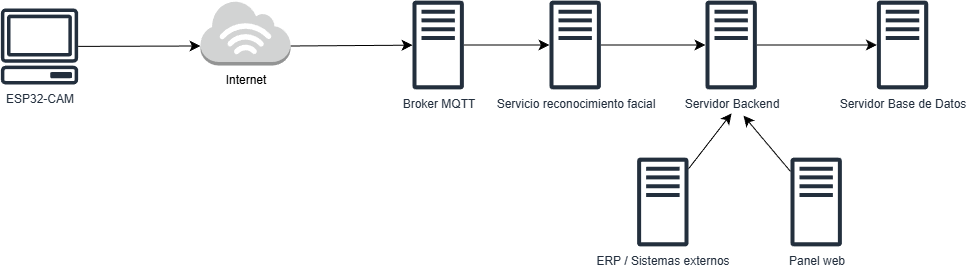
\includegraphics[width=\linewidth]{Imagenes/arqui2.drawio.png}
  \caption{Arquitectura física.}
  \label{fig:arq_fisica}
\end{figure}

\subsection{Arquitectura lógica}
Mientras que la arquitectura física muestra dónde corre cada servicio, la arquitectura lógica de la Fig.~\ref{fig:arq_logica} muestra cómo se organizan los módulos de software dentro de esos servicios y cómo se relacionan entre sí. En el lado del dispositivo, el ESP32-CAM agrupa cuatro módulos: la captura de imágenes (cámara OV2640), la lectura de huella (lector AS608 vía UART), el almacenamiento local en LittleFS (usuarios, turnos, asignaciones y asistencias en formato JSON) y el servidor web embebido que sirve la interfaz de configuración. Estos cuatro módulos no son independientes entre sí: por ejemplo, una marcación capturada por la cámara o el lector se guarda primero en LittleFS y solo después se intenta enviar al backend, lo que permite que el dispositivo siga funcionando aunque no haya conexión.

Del lado del servidor, el backend se organiza en blueprints de Flask (uno por dominio: personas, turnos, asistencias, dispositivos, ERP, etc.), cada uno con acceso a la base de datos PostgreSQL y, cuando corresponde, al servicio de reconocimiento facial. La comunicación entre el dispositivo y el backend ocurre por dos canales según el tipo de mensaje: MQTT para eventos de bajo volumen (heartbeats, comandos, resultados de enrolamiento) y HTTP para el envío de imágenes y la sincronización de datos. Esta separación de canales es la que permite que el dispositivo opere de forma autónoma cuando no hay red, almacene localmente lo que no pudo enviar, y sincronice todo una vez que la conexión se restablece.

\begin{figure}[H]
  \centering
  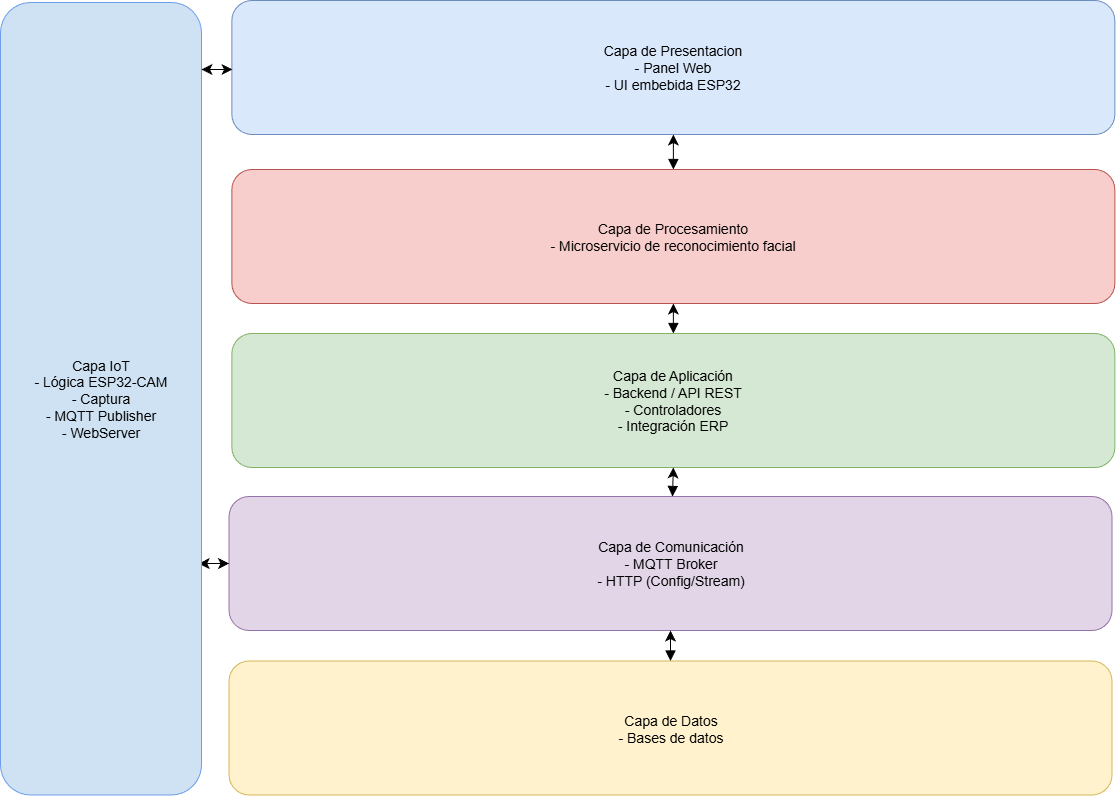
\includegraphics[width=.75\linewidth]{Imagenes/arquilogica.png}
  \caption{Arquitectura lógica.}
  \label{fig:arq_logica}
\end{figure}

La Fig.~\ref{fig:componentes_esp32} detalla, a nivel de hardware y firmware, los mismos cuatro módulos del ESP32-CAM descritos en la arquitectura lógica. En la capa de hardware se distinguen el microcontrolador ESP32, la cámara OV2640 (conectada por el bus paralelo DVP), el lector de huellas AS608 (conectado por UART) y el sensor PIR que activa la captura solo ante presencia detectada. En la capa de firmware, el servidor web embebido y el cliente MQTT comparten el acceso al sistema de archivos LittleFS, mientras que la máquina de estados central coordina cuándo se invoca cada módulo de captura biométrica según si el dispositivo está en modo de registro o de marcaje. Esta vista complementa a la Fig.~\ref{fig:arq_logica}, mostrando con qué pines y protocolos concretos se implementa cada bloque lógico.

\begin{figure}[H]
  \centering
  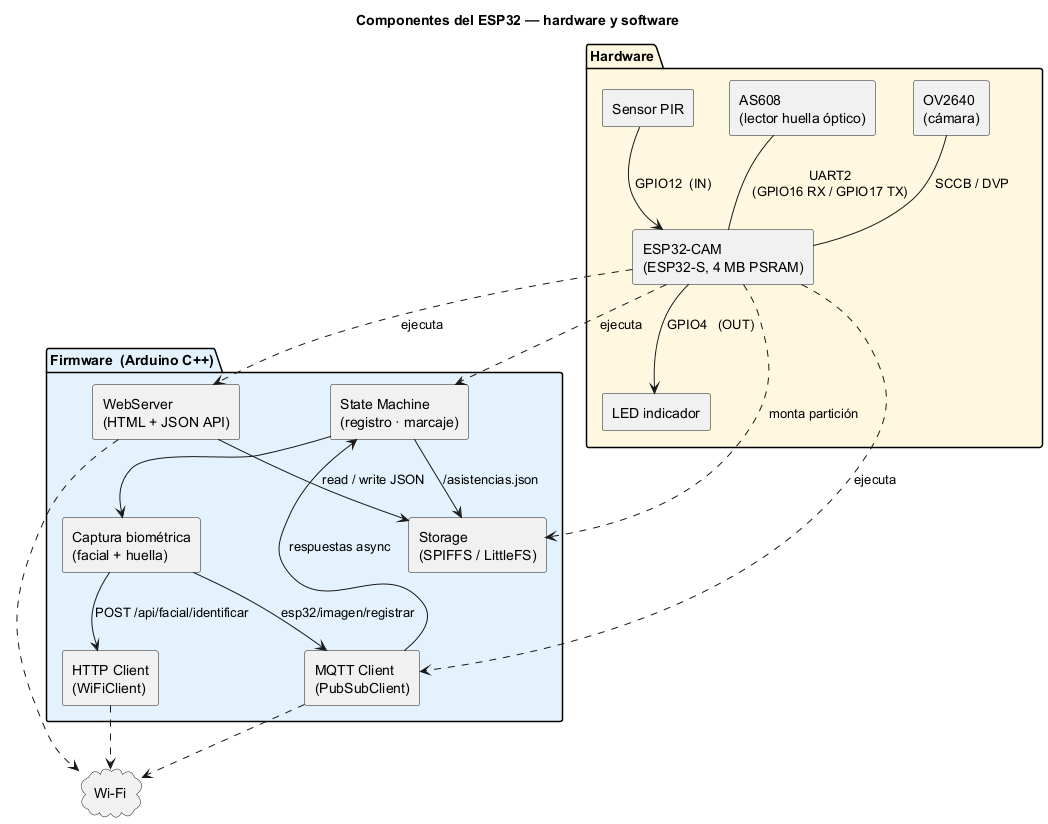
\includegraphics[width=\linewidth]{diagrams/componentes_esp32.png}
  \caption{Componentes del ESP32-CAM: hardware y firmware.}
  \label{fig:componentes_esp32}
\end{figure}

\section{Implementación}

En este apartado se procederá a explicar cómo se llevaron a cabo las iteraciones planteadas en el capítulo 3.1.

%% ============================================================
%% ITERACIÓN 1: Diseño y planificación inicial
%% ============================================================
\subsection{Iteración 1: Integración de hardware y servidor embebido}

La primera iteración corresponde al diseño conceptual del sistema y a la preparación del entorno de desarrollo, incluyendo la integración inicial del hardware biométrico seleccionado. Esta etapa establece la base funcional sobre la cual se construirán las iteraciones posteriores.

\subsubsection{Análisis}

En esta iteración se definieron los requisitos mínimos para validar la viabilidad técnica del sistema, analizando los componentes del hardware y las funcionalidades necesarias para las iteraciones siguientes.

El análisis se centró en tres ejes principales:

\begin{itemize}
    \item \textbf{Definición de funcionalidades mínimas (MVP)}:  
    Se identificaron las capacidades básicas que el dispositivo debía cumplir desde el inicio: capturar imágenes desde la cámara integrada, leer huellas dactilares mediante el sensor AS608, montar un servidor HTTP local con páginas HTML embebidas y operar de forma autónoma mediante Wi-Fi. Estas funciones representan la base operativa sobre la cual se desarrollarán características más avanzadas como turnos, sincronización y gestión de usuarios.

    \item \textbf{Identificación de limitaciones técnicas}:  
    Se revisaron las restricciones tecnológicas del ESP32-CAM, como la limitada memoria RAM disponible (~520 KB), el uso compartido del bus de cámara con los pines GPIO, la ausencia de pines GPIO libres -lo que forzó el uso de los pines GPIO14 (RX) y GPIO15 (TX) para la comunicación UART con el lector de huellas- y la necesidad de un manejo eficiente de cadenas HTML grandes en memoria. También se identificó que el flash LED integrado consume corriente significativa (~250 mA), requiriendo protección mediante PWM para evitar caídas de tensión durante la captura.

    \item \textbf{Estrategia de operación autónoma}:  
    Dado que uno de los requisitos fundamentales del sistema es la autonomía, se analizó la necesidad de montar un servidor web local. En caso de no contar con Wi-Fi configurada, el dispositivo debe activar automáticamente un modo Access Point (AP) con SSID ESP32-ASISTENCIA, permitiendo al administrador conectarse directamente para configurar la red y registrar usuarios sin dependencia de internet. Esto reduce riesgos y asegura la continuidad operacional del dispositivo.
\end{itemize}

Como resultado del análisis, se establecieron los criterios de diseño que guiarían el desarrollo de esta iteración: simplicidad, bajo consumo de recursos, modularidad de componentes y autonomía operativa.

\subsubsection{Diseño}

En esta iteración se elaboraron los primeros elementos arquitectónicos del sistema:

\begin{itemize}
    \item \textbf{Arquitectura física}, representando los componentes utilizados y su interconexión, la cual se puede revisar en la Fig.~\ref{fig:arq_fisica} de la sección 4.1.1.

    \item \textbf{Arquitectura lógica}, definiendo los módulos internos del firmware tales como captura de imágenes, lectura de huella, almacenamiento y conectividad, la cual se puede revisar en la Fig.~\ref{fig:arq_logica} de la sección 4.1.2.

    \item \textbf{Mockups iniciales} de la interfaz embebida del ESP32-CAM, incluyendo:

    \begin{itemize}
        \item Menú principal.
        \begin{figure}[H]
            \centering
            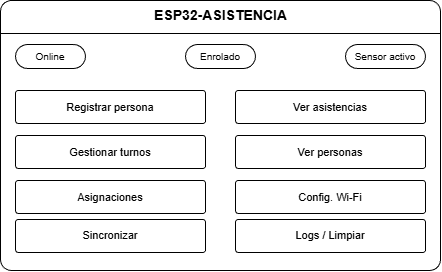
\includegraphics[width=.8\linewidth]{Imagenes/mockup_menu.png}
            \caption{Mockup menú principal en el ESP32-CAM.}
            \label{fig:mockup_menu}
        \end{figure}
        Wireframe inicial de la vista /: agrupa los indicadores de estado del dispositivo (conectividad, enrolamiento, sensor PIR) en la parte superior, y los accesos a cada módulo del sistema (registro, asistencias, turnos, personas, asignaciones, configuración Wi-Fi, sincronización y logs) como botones de navegación.

        \item Panel de configuración de Wi-Fi.
        \begin{figure}[H]
            \centering
            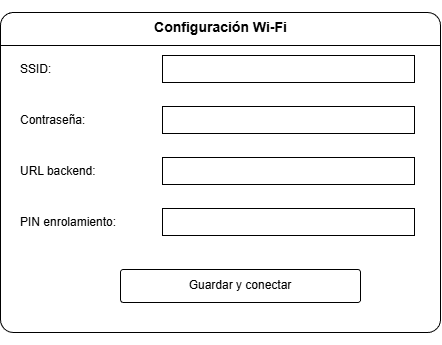
\includegraphics[width=.6\linewidth]{Imagenes/mockup_wifi.png}
            \caption{Mockup panel de configuración Wi-Fi.}
            \label{fig:mockup_wifi}
        \end{figure}
        Wireframe de la vista /wifi-setup: formulario con los cuatro campos que se persisten en wifi.json (SSID, contraseña de red, URL del backend y PIN de enrolamiento), accesible también desde el modo Access Point cuando el dispositivo no tiene credenciales configuradas.

        \item Vista de registro de usuario.
        \begin{figure}[H]
            \centering
            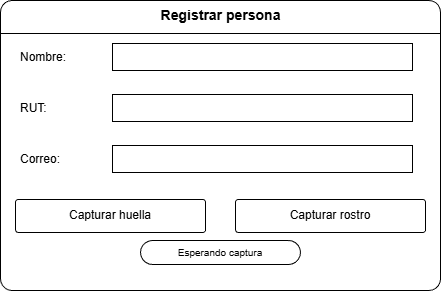
\includegraphics[width=.7\linewidth]{Imagenes/mockup_registro.png}
            \caption{Mockup registro de usuario en el ESP32-CAM.}
            \label{fig:mockup_registro}
        \end{figure}
        Wireframe de la vista /register: formulario de datos básicos (nombre, RUT, correo) seguido de los dos botones de captura biométrica, con un indicador de estado del proceso de enrolamiento (huella y rostro).

        \item Vista de usuarios almacenados localmente.
        \begin{figure}[H]
            \centering
            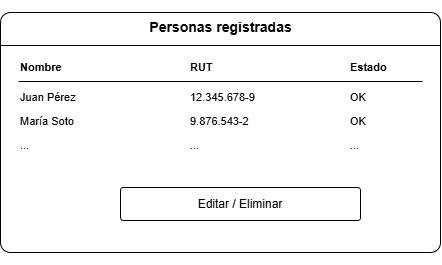
\includegraphics[width=.6\linewidth]{Imagenes/mockup_personas.png}
            \caption{Mockup de usuarios almacenados en el ESP32-CAM.}
            \label{fig:mockup_usuarios}
        \end{figure}
        Wireframe de la vista /personas: listado tabular de las personas registradas leídas desde personas.json, con acciones de edición y eliminación por fila.

        \item Vista de turnos almacenados localmente.
        \begin{figure}[H]
            \centering
            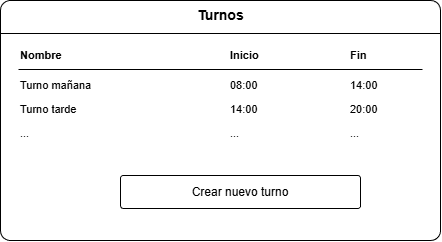
\includegraphics[width=.6\linewidth]{Imagenes/mockup_turnos.png}
            \caption{Mockup de visualización de turnos en el ESP32-CAM.}
            \label{fig:mockup_turnos}
        \end{figure}
        Wireframe de la vista /turnos: listado de los turnos almacenados en turnos.json, con el botón de acceso a la creación de un nuevo turno.

        \item Vista de crear turnos.
        \begin{figure}[H]
            \centering
            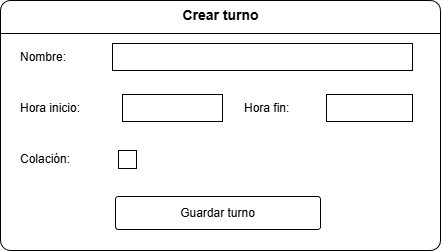
\includegraphics[width=.6\linewidth]{Imagenes/mockup_crear_turno.png}
            \caption{Mockup de creación de turnos en el ESP32-CAM.}
            \label{fig:mockup_crear_turnos}
        \end{figure}
        Wireframe de la vista /gestion: formulario para definir nombre, horario de inicio y fin, y la casilla opcional de colación que habilita los campos colacion\_inicio/colacion\_fin descritos en el Capítulo 4.

        \item Vista de asignación de turnos.
        \begin{figure}[H]
            \centering
            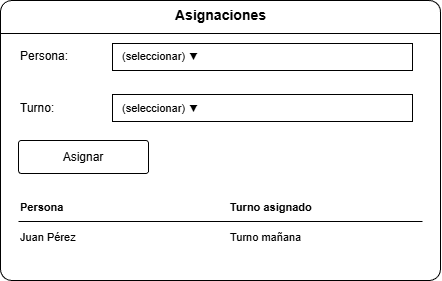
\includegraphics[width=.6\linewidth]{Imagenes/mockup_asignacion.png}
            \caption{Mockup de asignación de turnos en el ESP32-CAM.}
            \label{fig:mockup_asignacion}
        \end{figure}
        Wireframe de la vista /asignaciones: selección de persona y turno mediante listas desplegables, seguida del listado de asignaciones vigentes ya registradas.
    \end{itemize}

    \item \textbf{Diseño del flujo operacional}: a nivel conceptual, se planteó que el dispositivo debía capturar la huella o el rostro y luego evaluar si tenía conectividad disponible. Con conexión, la marcación se enviaría de inmediato al servidor; sin ella, se guardaría localmente para sincronizarse más adelante, cuando la red se restableciera. En ambos casos, la validación final (si la huella o el rostro corresponden a una persona registrada) ocurriría en el servidor, que respondería con un resultado de éxito o de error. El detalle de cómo se implementó cada uno de estos pasos, una vez que todos los componentes involucrados (enrolamiento, reconocimiento facial, sincronización diferida e integración ERP) estuvieron construidos, se presenta de forma consolidada al cierre del desarrollo, en la Sección~\ref{sec:flujo_operacional_consolidado}.
\end{itemize}

Estos elementos permiten visualizar el flujo básico del dispositivo antes de incorporar funcionalidades adicionales como turnos, sincronización o panel web backend, los cuales se desarrollarán en iteraciones posteriores.

\subsubsection{Implementación}

En esta etapa se integró tanto el hardware principal del prototipo como el desarrollo de las vistas web embebidas que permiten la interacción del usuario con el dispositivo. Para ello se utilizaron las siguientes librerías:

\begin{itemize}
    \item esp\_camera, utilizada para inicializar y configurar la cámara OV2640 integrada en el ESP32-CAM.
    \item HardwareSerial y Adafruit\_Fingerprint, empleadas para la comunicación UART con el lector biométrico AS608.
    \item WebServer, utilizada para montar un servidor web HTTP en el puerto 80 y atender rutas asociadas a las vistas.
    \item LittleFS y ArduinoJson \cite{arduinojson_docs}, empleadas para almacenamiento persistente en memoria flash y manipulación estructurada de datos JSON.
\end{itemize}

\paragraph{Integración del lector de huellas AS608}

El lector biométrico AS608 fue conectado directamente al ESP32-CAM mediante la interfaz UART secundaria (HardwareSerial 2), utilizando los pines GPIO14 (RX) y GPIO15 (TX). Esta conexión, que emplea pines distintos a los documentados inicialmente, fue forzada por la escasez de GPIO libres tras la asignación del bus de cámara. La velocidad de comunicación se estableció en 57600 baudios, y la librería Adafruit\_Fingerprint se vincula a dicho puerto serial. La Figura~\ref{fig:conexioneshuella} presenta la conexión física entre ambos dispositivos.

\begin{figure}[H]
    \centering
    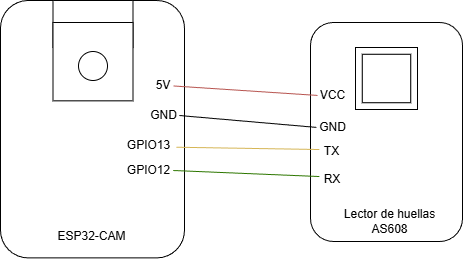
\includegraphics[width=.8\linewidth]{Imagenes/conexiones.png}
    \caption{Conexiones entre el ESP32-CAM y el lector de huellas AS608.}
    \label{fig:conexioneshuella}
\end{figure}

Una vez establecida la comunicación, el firmware puede ejecutar operaciones como:

\begin{itemize}
    \item Captura de imagen dactilar.
    \item Conversión de la imagen en una plantilla biométrica.
    \item Almacenamiento del template en un slot interno del sensor (1-127).
    \item Identificación mediante búsqueda de coincidencias en memoria.
\end{itemize}

La inicialización del lector se realiza con finger.begin(57600) sobre el puerto serie secundario, seguida de finger.verifyPassword() para confirmar que el sensor responde correctamente antes de habilitar las operaciones de captura, conversión y búsqueda descritas anteriormente.

\paragraph{Configuración de la cámara y el flash PWM}

La cámara OV2640 se configuró con resolución VGA (640×480) y compresión JPEG con calidad 8 (escala 0-63, donde valores bajos indican mayor calidad). La frecuencia del reloj externo (XCLK) se fijó en 20 MHz. Para evitar el parpadeo visible y las caídas de tensión provocadas por el flash LED durante la captura, se implementó un control PWM a 5 kHz con resolución de 8 bits, aplicando un ciclo de trabajo del 50\% (duty 128 de 255) durante la iluminación. Esto permite encender el flash con brillo suficiente sin sobrecargar la fuente de alimentación del ESP32-CAM.

\paragraph{Calibración del sensor PIR}

Se integró un sensor PIR (Passive Infrared) conectado al GPIO12 configurado con resistencia de pull-down interna. El sensor PIR actúa como detector de presencia: cuando una persona se sitúa frente al dispositivo, el PIR detecta el cambio de radiación infrarroja y activa el modo de captura. El setup incluye una fase de calibración de 3 segundos para estabilizar la lectura del sensor antes de iniciar el bucle principal. La lógica de uso del PIR como control de activación se detalla en la iteración 6.

\paragraph{Montaje del servidor web embebido}

Para habilitar la interacción local con el dispositivo, se implementó un servidor web mediante la librería WebServer en el puerto 80. Este servidor permite entregar páginas HTML, datos JSON y recursos estáticos. Cuando no hay conectividad a una red externa, el ESP32-CAM activa automáticamente un Access Point con SSID ESP32-ASISTENCIA y contraseña Asistencia2026, sirviendo las mismas páginas sin depender de internet.

Las rutas principales del sistema incluyen:

\begin{itemize}
    \item /: Menú principal con indicadores de estado.
    \item /wifi-setup: Configuración de red Wi-Fi y parámetros del backend.
    \item /register: Registro de personas con captura biométrica.
    \item /asistencias: Lista de asistencias almacenadas localmente.
    \item /gestion: Gestión de turnos (creación y administración).
    \item /personas: Visualización de personas registradas.
    \item /asignaciones: Vista para realizar asignaciones de turnos.
    \item /logs: Visualización de logs del sistema.
    \item /turnos: Visualización de turnos creados.
\end{itemize}

Para la implementación del servidor HTTP embebido, se utilizó el módulo WebServer del ESP32. Cada operación del sistema (registro de usuarios, captura de huellas, creación de turnos, asignación de turnos, lectura de asistencias, configuración Wi-Fi, entre otras) fue mapeada a un endpoint específico mediante funciones manejadoras (handler functions), registradas mediante "server.on(ruta, metodo, handler)" para cada una de las rutas listadas anteriormente. Este mecanismo permite encapsular la lógica de cada componente del sistema y mantener una estructura modular del firmware.

\paragraph{Creación de vistas HTML embebidas}

Las vistas fueron desarrolladas como archivos .html independientes almacenados en el sistema de archivos LittleFS del ESP32-CAM, conteniendo HTML, CSS y JavaScript autónomo, sin dependencias de CDN externas. El servidor web embebido las sirve mediante la función servirArchivo(), que lee el archivo solicitado desde LittleFS y lo envía al cliente. Esto garantiza que el ESP32-CAM sirva cada página incluso en modo Access Point sin conexión a internet.

\paragraph{Menú principal}

La Figura~\ref{fig:menu_principal} presenta la vista principal accesible en la ruta /. Desde esta interfaz el usuario puede visualizar el estado del dispositivo (online/offline, sensor activo, enrolado), registrar personas, ver asistencias, gestionar turnos, ver asignaciones, acceder a la configuración de red, sincronizar con el backend y limpiar datos del dispositivo. Con el avance de las iteraciones se agregaron a esta vista los indicadores de estado que se actualizan cada pocos segundos consultando al dispositivo, un bloque para mostrar el PIN de registro que permanece oculto hasta que el usuario decide revelarlo, una zona separada para las acciones de reinicio y borrado total de datos, y la opción de proteger la página con contraseña de administrador cuando se requiere restringir el acceso a esas acciones.

\begin{figure}[H]
    \centering
    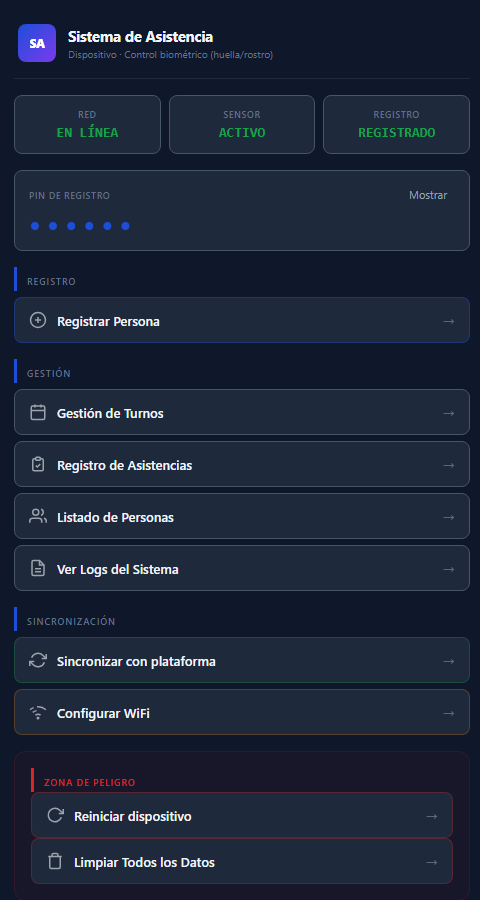
\includegraphics[height=8.5cm,keepaspectratio]{Imagenes/menuimplementado.png}
    \caption{Menú principal del sistema web embebido.}
\label{fig:menu_principal}
\end{figure}

\paragraph{Vista de configuración Wi-Fi}

Mediante la ruta /wifi-setup, el dispositivo proporciona un formulario para actualizar las credenciales de la red local (SSID, contraseña), la URL del backend, la dirección del broker MQTT y el PIN de enrolamiento. Estos valores se persisten en SPIFFS mediante el archivo wifi.json. La Figura~\ref{fig:wifi_config} muestra esta interfaz. Por requerimientos de seguridad identificados en iteraciones posteriores, se agregó a esta vista la opción de forzar conexiones cifradas hacia el backend y el broker MQTT, además de un apartado donde se puede definir o cambiar la contraseña de administrador pidiendo la contraseña actual como confirmación, de modo que no cualquier persona con acceso a la red local pueda modificar la configuración del dispositivo.

\begin{figure}[H]
    \centering
    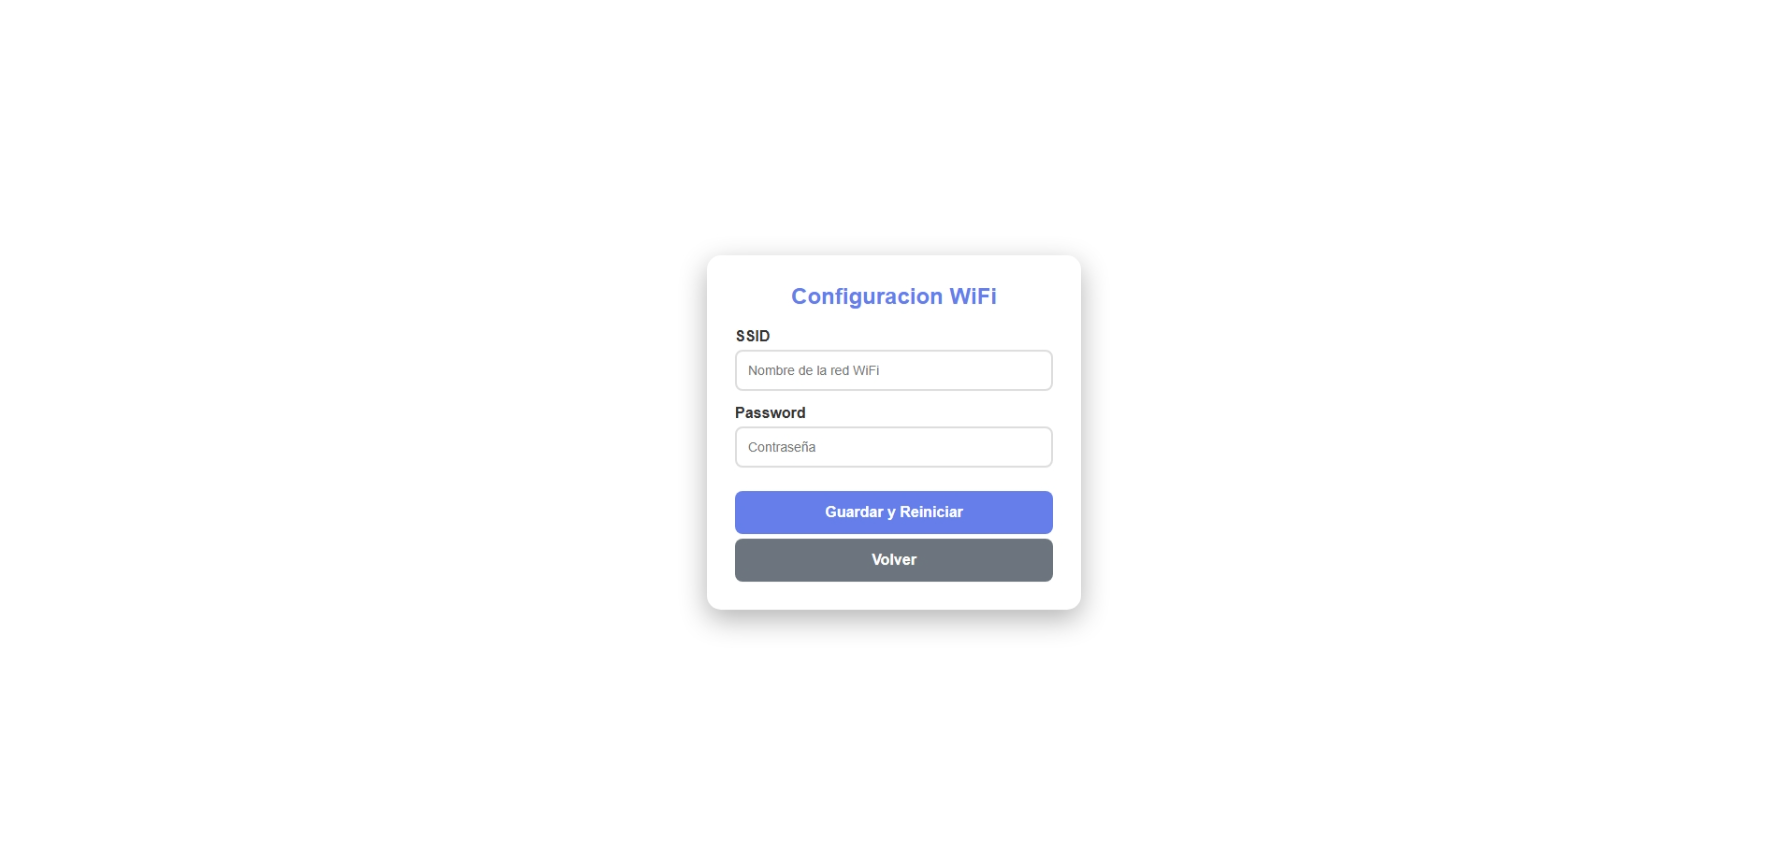
\includegraphics[height=8.5cm,keepaspectratio]{Imagenes/menuwifiimplementado.png}
    \caption{Interfaz de configuración Wi-Fi.}
\label{fig:wifi_config}
\end{figure}

\paragraph{Vista de registro de personas}

La ruta /register despliega una vista que combina un formulario para ingresar el nombre del usuario, RUT y correo electrónico, y muestra indicadores visuales del estado del proceso de enrolamiento (huella, rostro). La Figura~\ref{fig:registro_personas} lo muestra. Se incorporó a esta vista una casilla de consentimiento explícito para el tratamiento de datos biométricos, exigida por las consideraciones éticas y de privacidad descritas en el marco metodológico; mientras no se marque, el botón para iniciar el registro biométrico queda deshabilitado. El flujo se complementó además con un panel que informa el avance del proceso y con una pantalla de captura facial guiada, que muestra cuántas de las tres fotografías necesarias para el reconocimiento facial ya se han tomado.

\begin{figure}[H]
    \centering
    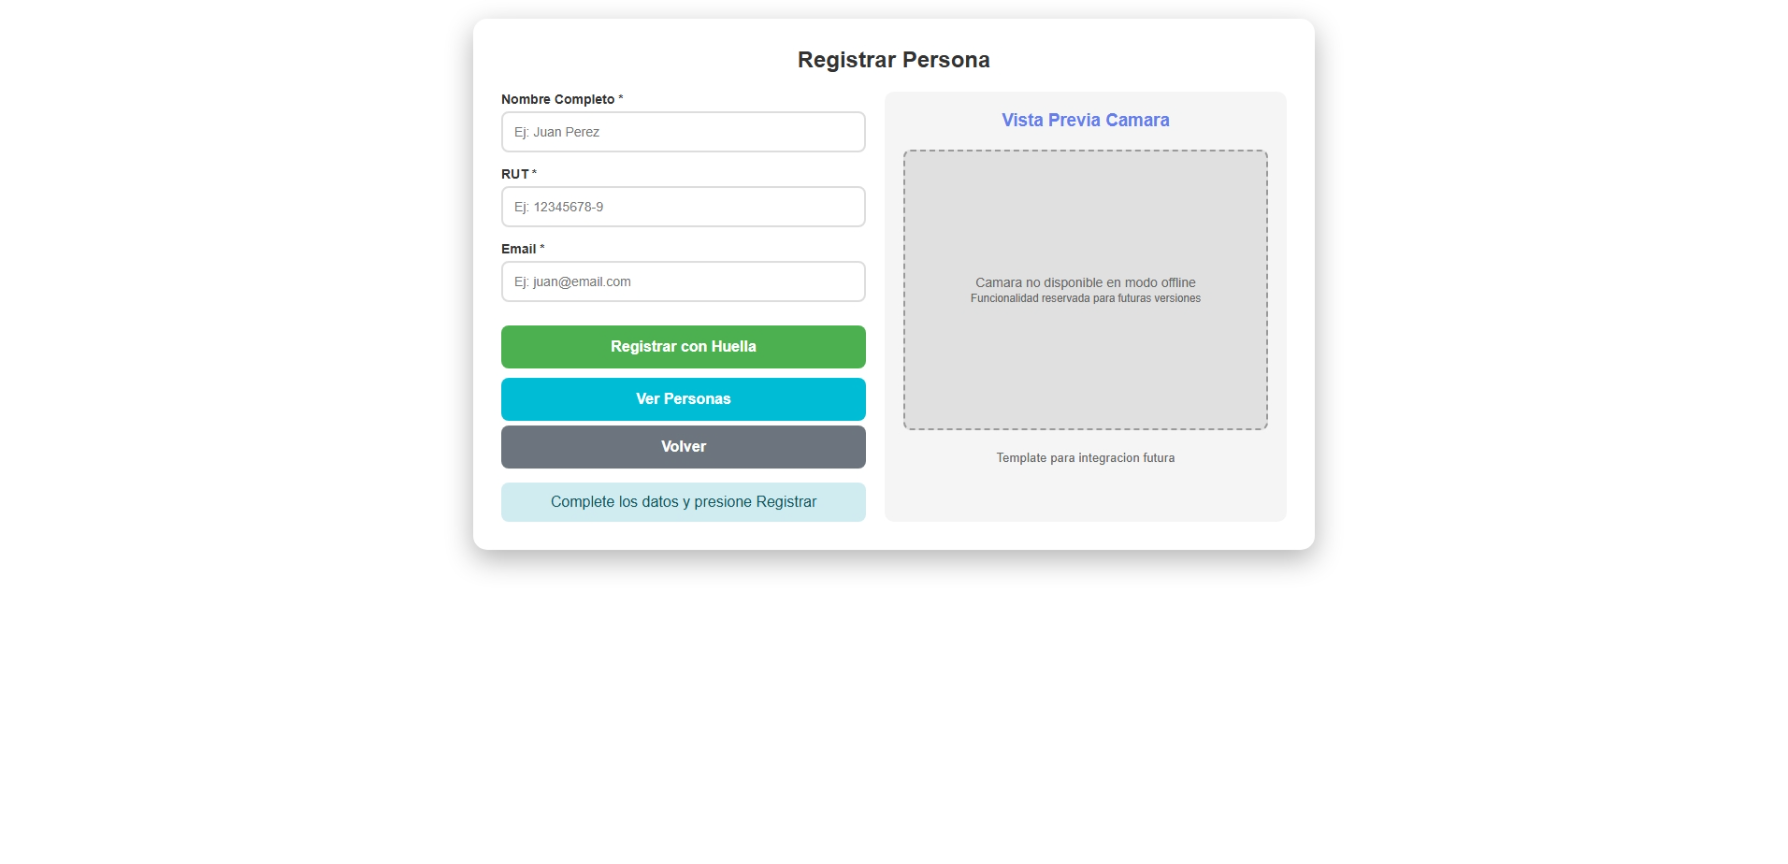
\includegraphics[height=8.5cm,keepaspectratio]{Imagenes/registroimplementado.png}
    \caption{Vista para el registro de personas en el dispositivo.}
\label{fig:registro_personas}
\end{figure}

\paragraph{Vista de asistencias}

Para visualizar registros de asistencia tanto locales como sincronizados, se implementó la vista en la ruta /asistencias. Esta consulta archivos JSON almacenados en LittleFS. La Figura~\ref{fig:vista_asistencias} lo ejemplifica. Cada registro se presenta como una tarjeta diferenciada por color según sea entrada o salida, con el nombre de la persona, la marca de tiempo y su identificador asociado. A la versión inicial, que solo listaba los registros, se le agregaron las opciones de editar o eliminar cada fila, pensadas para que el encargado de turno pueda corregir una marcación errónea, como una doble lectura biométrica, sin necesidad de acceder directamente al backend. También se sumó un contador de registros totales en la parte superior, útil para revisar de un vistazo cuántos datos hay almacenados localmente antes de sincronizar.

\begin{figure}[H]
    \centering
    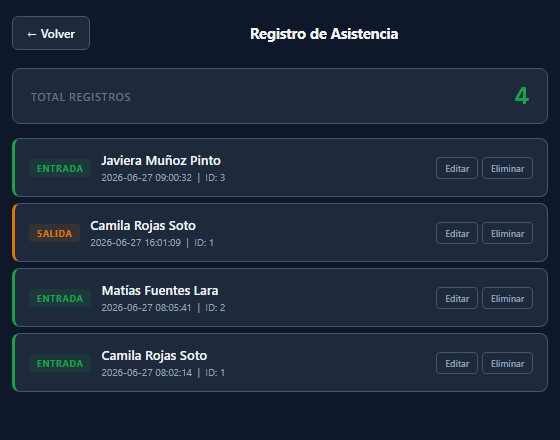
\includegraphics[height=8.5cm,keepaspectratio]{Imagenes/vistaasitenciasimplementado.png}
    \caption{Vista de asistencias locales almacenadas en el dispositivo.}
\label{fig:vista_asistencias}
\end{figure}

\paragraph{Vista de Personas registradas}

Para visualizar las personas registradas, se implementó la vista en la ruta /personas. Esta consulta archivos JSON almacenados en LittleFS y permite editar nombre/correo, actualizar huella o rostro, y eliminar personas. La Figura~\ref{fig:personas_registradas} lo ejemplifica. Las opciones para actualizar la huella o el rostro, y para agregar fotos adicionales, se incorporaron después de notar en las pruebas de campo que volver a registrar a una persona desde cero, borrando y repitiendo todo el proceso, tomaba demasiado tiempo. Con estas opciones se puede corregir solo la huella o el rostro de alguien ya registrado, o sumar fotos para mejorar el reconocimiento facial, sin perder el resto de sus datos ni su historial de asistencia.

\begin{figure}[H]
    \centering
    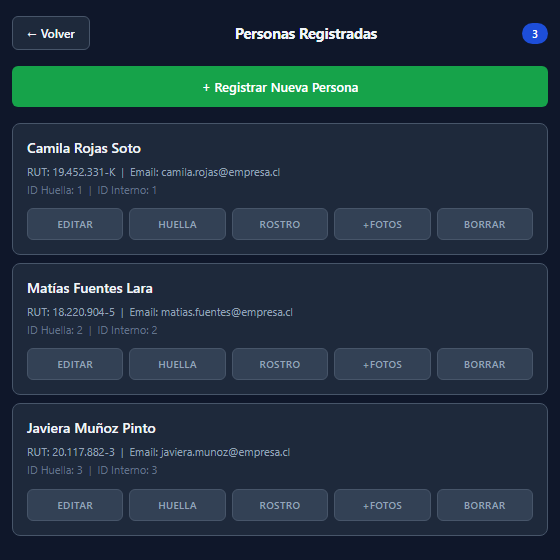
\includegraphics[height=8.5cm,keepaspectratio]{Imagenes/personasregistradasimplementada.png}
    \caption{Vista de personas registradas en el dispositivo.}
\label{fig:personas_registradas}
\end{figure}

\paragraph{Vista de Crear Turnos}

Para la creación de turnos y visualización de los existentes, se implementó la vista en la ruta /gestion, complementada con /turnos. Estas consultan archivos JSON almacenados en LittleFS. La Figura~\ref{fig:gestion_turnos} lo ejemplifica. La vista /gestion funciona como panel resumen, con accesos directos a la gestión de turnos, a las asignaciones y a la sincronización manual con la plataforma. La vista /turnos concentra el formulario para crear un turno nuevo, con nombre, hora de inicio y fin, y un selector de días de la semana, junto con el listado editable de los turnos ya creados. Esta separación entre resumen y edición se introdujo para que las modificaciones no ocurran por accidente desde la pantalla que se usa con más frecuencia.

\begin{figure}[H]
    \centering
    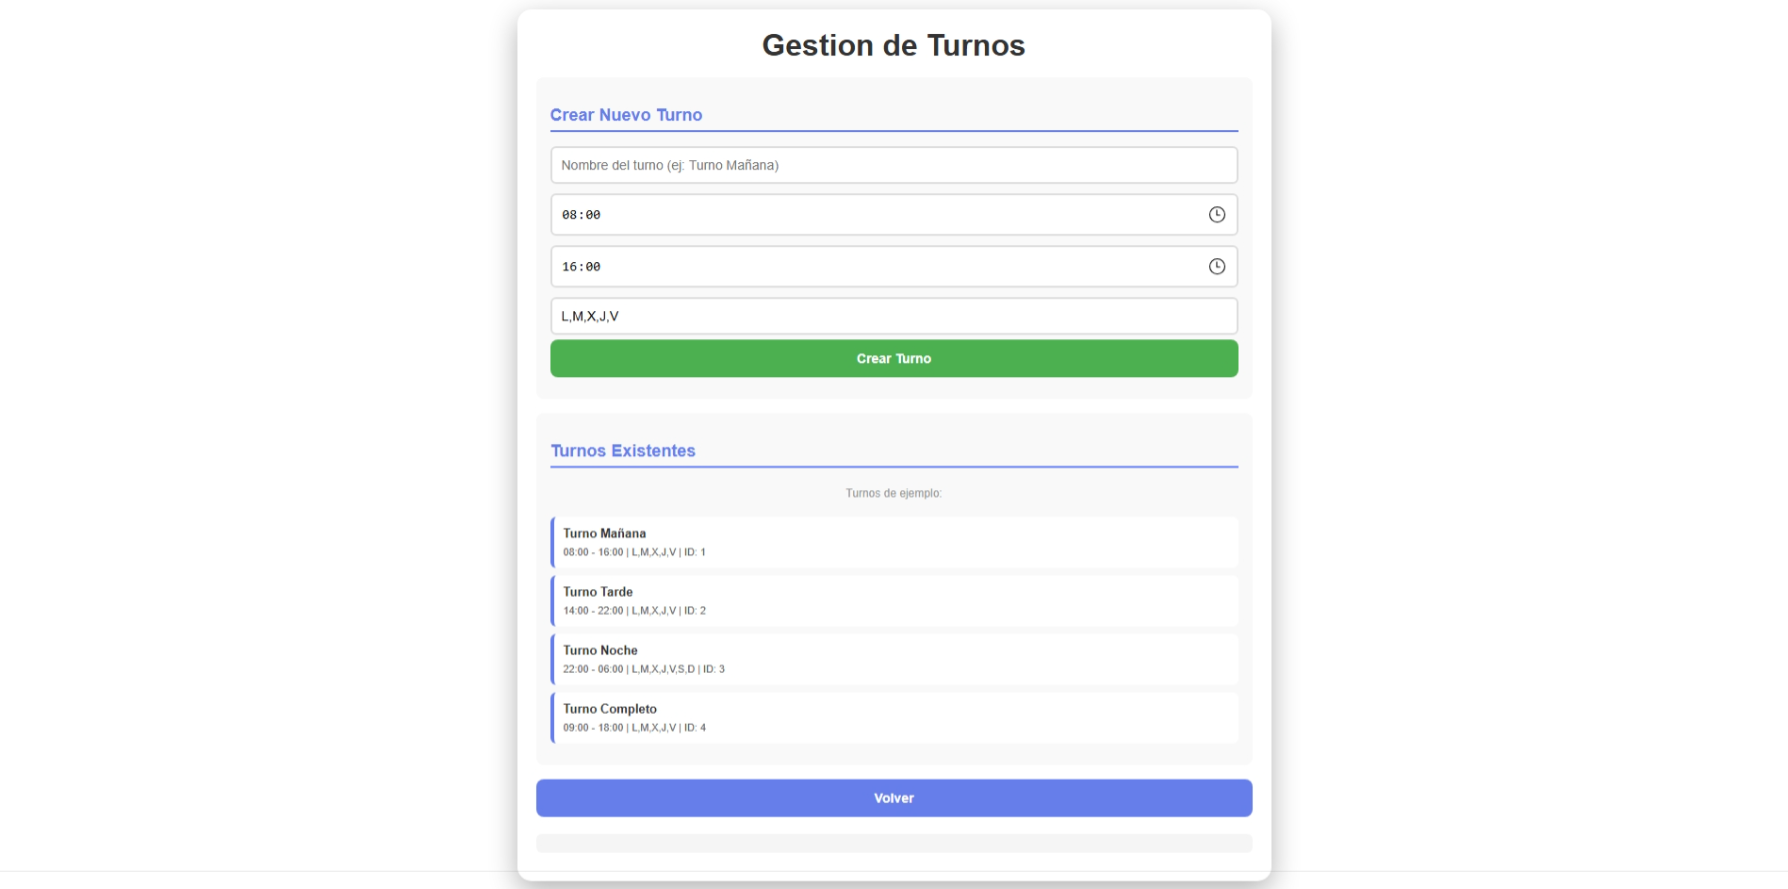
\includegraphics[height=8.5cm,keepaspectratio]{Imagenes/creacionturnos.png}
    \caption{Vista de gestión y creación de turnos en el dispositivo.}
\label{fig:gestion_turnos}
\end{figure}

\paragraph{Vista de asignación de turnos}

Para visualizar las asignaciones de turnos y realizar la acción de asignar un turno a una persona, se implementó la vista en la ruta /asignaciones. La Figura~\ref{fig:asignacion_turnos} lo ejemplifica. El formulario superior permite elegir una persona y un turno ya creados desde listas desplegables, evitando que el usuario tenga que recordar o escribir identificadores internos. El listado de asignaciones actuales muestra el nombre de la persona y del turno en lugar de solo sus identificadores, e incluye una opción para quitar una asignación, agregada después de notar que reasignar turnos por cambios de horario del personal era algo que ocurría seguido durante el uso del prototipo.

\begin{figure}[H]
    \centering
    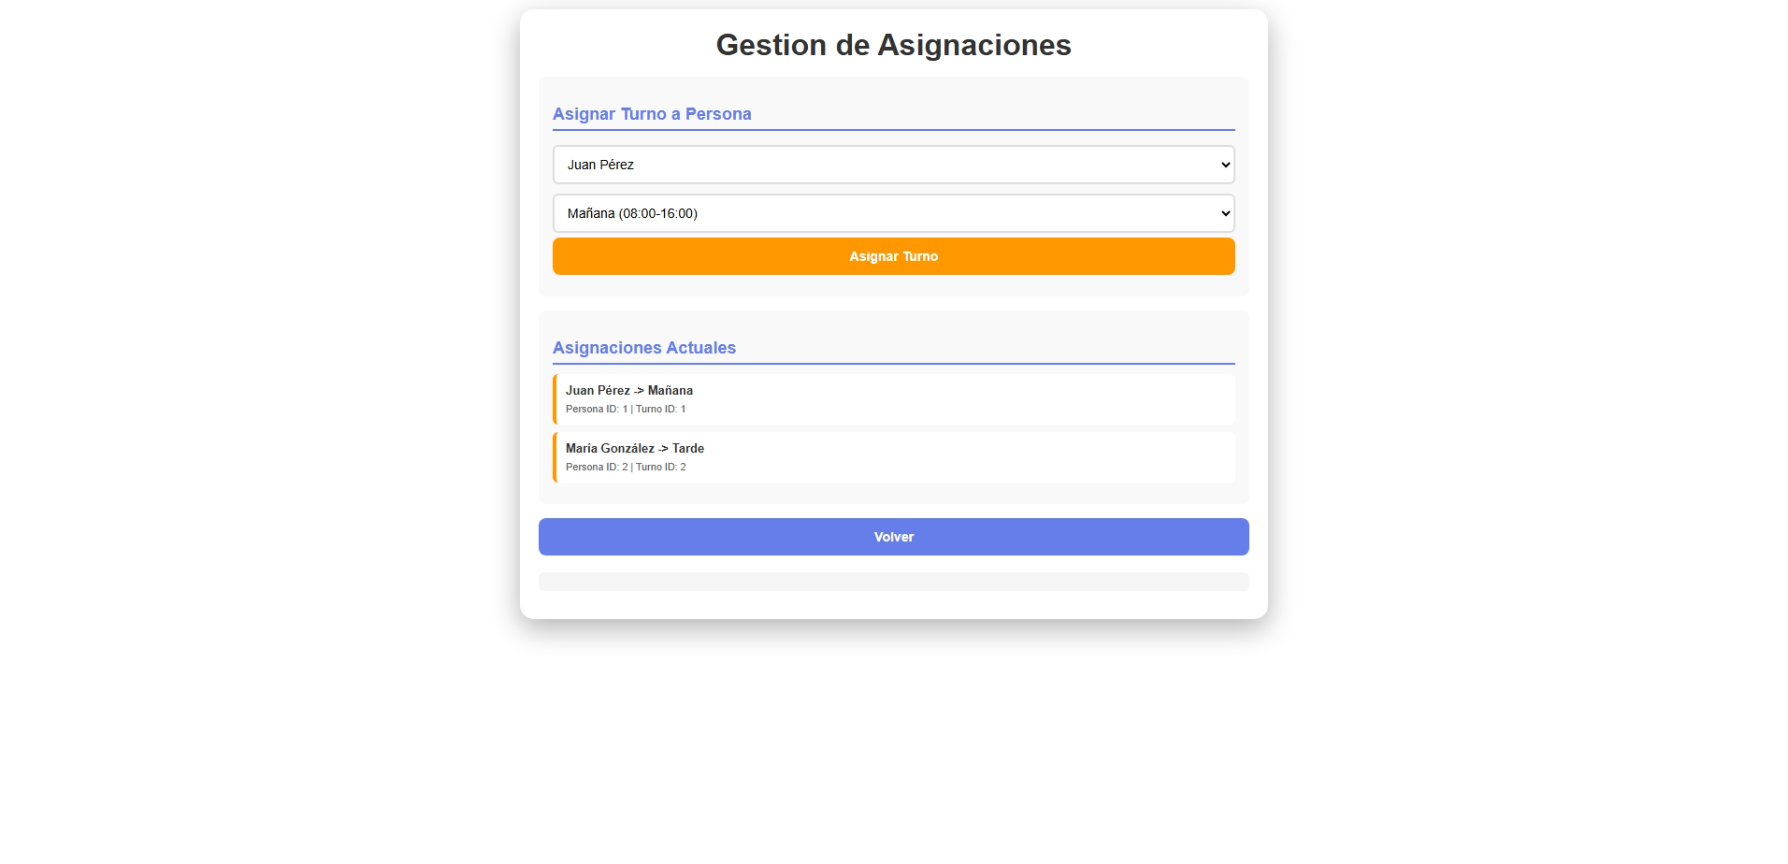
\includegraphics[height=8.5cm,keepaspectratio]{Imagenes/asignacionturnoimplementacion.png}
    \caption{Vista de gestión de asignaciones en el dispositivo.}
\label{fig:asignacion_turnos}
\end{figure}

\subsubsection{Pruebas}

Para validar el funcionamiento del prototipo y comprobar la correcta integración entre los distintos módulos del sistema, se diseñaron pruebas de integración enfocadas exclusivamente en los componentes implementados durante esta iteración:

\begin{itemize}
    \item \textbf{Prueba de captura de imágenes}: Verificar que la cámara OV2640 capture imágenes JPEG de forma continua y estable, sin corrupción de frames ni errores de inicialización del sensor. Se espera que la función esp\_camera\_fb\_get() retorne buffers consistentes tras cada llamada.

    \item \textbf{Prueba de comunicación UART con AS608}: Verificar que el lector biométrico responda correctamente al comando de verificación de contraseña (finger.verifyPassword()) y que la comunicación serie a 57600 baudios se establezca sin pérdida de paquetes. Se espera confirmación de conexión en menos de 1 segundo tras el inicio.

    \item \textbf{Prueba de lectura biométrica}: Verificar que el AS608 pueda capturar una imagen dactilar (finger.getImage()), convertirla a plantilla (finger.image2Tz()) y almacenarla en un slot del sensor (finger.storeModel()). Se espera que el proceso completo tome menos de 2 segundos.

    \item \textbf{Prueba de acceso vía AP}: Verificar que al iniciar sin credenciales Wi-Fi configuradas, el ESP32-CAM active el Access Point ESP32-ASISTENCIA y que las páginas HTML sean accesibles desde un navegador conectado a la IP 192.168.4.1. Se espera que todas las rutas definidas respondan con código HTTP 200.

    \item \textbf{Prueba de carga de vistas vía Wi-Fi externa}: Verificar que al conectar el dispositivo a una red Wi-Fi configurada, las mismas vistas se carguen correctamente a través de la IP asignada por el router, manteniendo estilos, scripts y funcionalidad.
\end{itemize}

\subsubsection{Refinamientos posteriores}

Durante el desarrollo de las iteraciones siguientes surgieron dos problemas asociados a la base construida en esta etapa, los cuales fueron corregidos durante el mismo ciclo de implementación.

El primero se presentó al combinar las funcionalidades de conectividad y enrolamiento: un dispositivo podía encontrarse conectado a internet sin contar aún con una persona enrolada, o bien tener una persona enrolada pero haber perdido la conexión de red. En ambos casos, el firmware intentaba ejecutar la sincronización o el reconocimiento facial de igual forma, lo que provocaba fallos sin generar un mensaje de error claro para el usuario. Para resolver esta situación, se implementó una función de validación que verifica simultáneamente ambas condiciones antes de permitir cualquier operación dependiente del backend, evitando así que el dispositivo ejecute procesos que se sabe resultarán en error.

El segundo ajuste estuvo relacionado con la calidad de las imágenes utilizadas para el reconocimiento facial. Las capturas estándar de la cámara se almacenaban con un nivel de compresión orientado a vistas previas rápidas, el cual resultaba insuficiente para generar un embedding facial de calidad adecuada, debido a la pérdida de detalle en los rasgos del rostro. Por este motivo, se diferenció el proceso de captura correspondiente al registro biométrico, incrementando temporalmente la resolución del sensor exclusivamente para la fotografía de referencia, y restableciéndola a su configuración estándar una vez completada la captura, sin afectar el resto de las imágenes procesadas por el sistema.

%% ============================================================
%% ITERACIÓN 2: Almacenamiento local y modo offline
%% ============================================================

\subsection{Iteración 2: Almacenamiento local y modo offline}

La segunda iteración se centra en habilitar el funcionamiento autónomo del dispositivo sin conexión a internet, integrando un sistema de almacenamiento persistente basado en LittleFS (sucesor moderno de SPIFFS para ESP32) y los mecanismos de captura biométrica offline. Esta etapa materializa lo definido en el apartado 3.1.2 del capítulo anterior.

\subsubsection{Análisis}

Para el correcto funcionamiento offline del prototipo se identificaron los siguientes requerimientos:

\begin{itemize}
    \item Almacenar localmente los datos de usuarios, turnos, asignaciones y asistencias en formato JSON.
    \item Permitir el registro de marcaciones aun cuando no exista conectividad externa, tanto por huella (offline total) como con validación de turnos locales.
    \item Garantizar persistencia de la información tras reinicios del ESP32-CAM o cortes de energía.
    \item Habilitar la gestión completa del sistema mediante una interfaz web embebida accesible vía Access Point.
    \item Mantener compatibilidad con la futura sincronización automática en modo online, marcando cada registro con un campo sincronizado (booleano) para su posterior envío al backend.
\end{itemize}

Para cumplir estos requisitos se seleccionó el sistema de archivos LittleFS y el formato JSON debido a su bajo peso, facilidad de manipulación mediante la librería ArduinoJson y compatibilidad con las capacidades del ESP32-CAM (4 MB de flash, de los cuales aproximadamente 1.5 MB están disponibles para LittleFS). Adicionalmente, se definió un archivo de configuración, wifi.json, destinado a almacenar credenciales Wi-Fi, URL del backend, dirección del broker MQTT y PIN de enrolamiento.

\subsubsection{Diseño}

Considerando la arquitectura establecida, se diseñaron las siguientes estructuras de almacenamiento en formato JSON:

\begin{itemize}
    \item \textbf{personas.json}: Arreglo de objetos con campos id, nombre, rut, email, huella\_id, fecha\_registro, sincronizado.
    \item \textbf{turnos.json}: Arreglo de objetos con campos id, backend\_id, nombre, inicio, fin, dias, sincronizado.
    \item \textbf{asignaciones.json}: Arreglo de objetos con campos persona\_id, turno\_id, backend\_id, fecha\_asignacion, sincronizado.
    \item \textbf{asistencias.json}: Arreglo de objetos con campos persona\_id, nombre, tipo (entrada/salida), metodo (huella\_offline, facial, etc.), timestamp, sincronizado.
    \item \textbf{wifi.json}: Objeto con campos ssid, pass, backend, mqtt, pin (para enrolamiento del dispositivo).
    \item \textbf{erp-config.json}: Arreglo con configuraciones de integraciones ERP, sincronizado desde el backend cuando hay conectividad.
\end{itemize}

El campo sincronizado (booleano) en cada entidad actúa como bandera para el proceso de sincronización diferida: cuando el dispositivo recupera conectividad, itera sobre los registros con sincronizado = false y los envía al backend. Una vez confirmada la recepción, se marca sincronizado = true.

\subsubsection{Implementación}

En esta iteración se integraron las librerías LittleFS, ArduinoJson, HardwareSerial y Adafruit\_Fingerprint. Las dos primeras permiten gestionar archivos JSON alojados en la memoria flash del ESP32-CAM, mientras que las dos últimas habilitan la comunicación UART con el lector biométrico AS608 para el registro y verificación de huellas digitales.

\paragraph{Inicialización del sistema de archivos y persistencia}

El primer componente de la implementación consiste en montar LittleFS mediante LittleFS.begin(true) y verificar la existencia de los archivos necesarios. En caso de no existir, el sistema los crea con una estructura inicial vacía (arreglo [] para las colecciones, objeto con valores por defecto para wifi.json), asegurando que el dispositivo pueda operar incluso tras un primer arranque sin configuración previa.

Se implementaron dos funciones genéricas para la manipulación de archivos JSON:

\begin{itemize}
    \item loadArray(const char* path, DynamicJsonDocument\& doc): Abre un archivo, deserializa su contenido como JsonArray y lo retorna. Si el archivo no existe o está corrupto, retorna un arreglo vacío.
    \item saveArray(const char* path, DynamicJsonDocument\& doc): Serializa el documento JSON y lo escribe en el archivo correspondiente, sobrescribiendo el contenido anterior.
\end{itemize}

Estas funciones encapsulan toda la lógica de persistencia del sistema y son reutilizadas por todos los módulos que necesiten leer o escribir datos.

El tamaño de cada DynamicJsonDocument se dimensionó según el volumen esperado de datos de cada archivo, aunque varía según la función que lo utiliza: asignaciones.json utiliza típicamente 1024~bytes, personas.json y turnos.json se manejan con buffers de entre 2048 y 8192~bytes dependiendo del contexto (lectura local, sincronización o registro), y asistencias.json utiliza 32768~bytes. Adicionalmente, en la función procesarAsistencia() se incorporó una validación sobre el retorno de createNestedObject(): si el objeto retornado es nulo (indicando desbordamiento del documento), se registra una advertencia en el log del sistema, permitiendo detectar tempranamente cuellos de botella de memoria sin comprometer la integridad del archivo JSON. El dimensionamiento de este buffer y la estrategia adoptada para sostener el volumen de registros exigido en los objetivos del proyecto se detallan en el apartado de refinamientos posteriores de esta iteración.

\paragraph{Registro de usuarios con huella digital}

El registro de usuarios se implementó mediante un flujo que combina la captura biométrica gestionada por el lector AS608 con el almacenamiento en personas.json. El lector administra internamente modelos de huellas mediante \textit{slots} numerados del 1 al 127. Por ello, antes del enrolamiento es necesario identificar un slot disponible dentro del sensor. La función encontrarSlotLibre() recorre el arreglo de personas, determina el ID de huella más alto registrado y retorna el siguiente disponible.

Una vez encontrado un slot, se ejecuta el proceso de enrolamiento en dos fases:

\begin{enumerate}
    \item \textbf{Primera captura} (ESTADO\_ESPERANDO\_HUELLA\_REGISTRO): El sistema espera que el usuario coloque el dedo. Al detectar una imagen válida, la convierte a plantilla en el buffer 1 y transiciona a ESTADO\_ESPERANDO\_SOLTAR\_DEDO.
    \item \textbf{Espera y segunda captura} (ESTADO\_REGISTRO\_SEGUNDA\_HUELLA): Una vez que el sensor detecta que el dedo fue retirado (FINGERPRINT\_NOFINGER), el sistema solicita una segunda captura del mismo dedo. Al obtenerla, convierte a plantilla en el buffer 2, crea el modelo combinado (finger.createModel()) y lo almacena en el slot correspondiente (finger.storeModel()).
\end{enumerate}

Luego del enrolamiento exitoso, se almacena un nuevo objeto dentro de personas.json con un identificador único (generado localmente con prefijo local- o provisto por el backend si hay conectividad), el nombre, RUT, correo electrónico y el slot asignado. La etapa de captura de huella aquí descrita corresponde a los primeros estados de la máquina de estados del registro biométrico completo, presentada más adelante en la Figura~\ref{fig:maquina_estados_esp32} (sección 4.3.4), una vez introducido el envío de la foto de referencia al backend por HTTP.

\paragraph{Registro de asistencia en modo offline}

El registro de asistencia se realiza completamente en el dispositivo, sin necesidad de conexión externa. El flujo implementado consiste en:

\begin{enumerate}
    \item Capturar una huella mediante el lector AS608 (finger.getImage()).
    \item Convertir la imagen a plantilla (finger.image2Tz()) y ejecutar una búsqueda biométrica (finger.fingerSearch()) que retorna el fingerID del slot coincidente.
    \item Identificar al usuario asociado mediante el campo huella\_id en personas.json con la función buscarPersonaPorHuella().
    \item Verificar que el usuario cuente con un turno asignado consultando asignaciones.json mediante turnoActivo(). Si no tiene turno, el sistema rechaza la marcación.
    \item Determinar el tipo de evento (entrada/salida) alternando automáticamente respecto al último registro de la persona en asistencias.json.
    \item Generar un nuevo registro con sincronizado = false (salvo que se logre enviar al backend en ese momento).
\end{enumerate}

El manejador handleMarcarAsistencia() expone esta funcionalidad a través de la interfaz web, permitiendo también marcaciones manuales. El escaneo automático continuo se controla mediante intervalos configurables: 2 segundos entre verificaciones de huella y 6 segundos entre verificaciones faciales.

\paragraph{Gestión de turnos y asignaciones}

Además del registro de asistencias, el sistema permite crear turnos (handleCreateTurn()) y asignarlos a personas (handleAssignTurn()) desde la interfaz web. Cada operación persiste los datos en sus archivos JSON correspondientes y, si hay conectividad, intenta replicar la operación en el backend mediante HTTP POST.

\paragraph{Operación offline del dispositivo}

Con el objetivo de asegurar autonomía total, el ESP32-CAM fue configurado para operar en dos modos:

\begin{itemize}
    \item \textbf{Modo Wi-Fi STA}: Si hay credenciales configuradas en wifi.json, el dispositivo intenta conectarse a la red externa. Si la conexión falla reiteradamente (5 intentos), activa el modo AP como fallback sin deshabilitar el intento de reconexión.
    \item \textbf{Modo Access Point}: El punto de acceso utiliza el SSID ESP32-ASISTENCIA y contraseña Asistencia2026, permitiendo que un administrador se conecte directamente al dispositivo en la IP 192.168.4.1 para realizar todas las operaciones mediante la interfaz web embebida.
\end{itemize}

\subsubsection{Pruebas}

Se diseñaron las siguientes pruebas para validar el correcto funcionamiento del almacenamiento local y el modo offline:

\begin{itemize}
    \item \textbf{Prueba de persistencia tras reinicio}: Registrar usuarios, turnos, asignaciones y asistencias, luego reiniciar el ESP32-CAM (por corte de energía o comando software). Verificar que todos los archivos JSON conserven su contenido íntegro y que el sistema pueda leerlos correctamente tras el reinicio.

    \item \textbf{Prueba de lectura y deserialización}: Abrir cada archivo JSON generado y verificar que ArduinoJson pueda deserializar su contenido sin errores ni pérdida de campos. El tamaño de cada DynamicJsonDocument se configuró según la capacidad esperada del archivo: 2048~bytes para personas.json y turnos.json, 1024~bytes para asignaciones.json y 32768~bytes para asistencias.json. Se incluyó además una validación post-inserción (mediante isNull()) en la función procesarAsistencia() para detectar y registrar en logs cualquier desbordamiento del documento al crear nuevos registros de asistencia.

    \item \textbf{Prueba de escritura concurrente}: Realizar múltiples operaciones de escritura (registro de persona + asignación de turno + marcación de asistencia) en rápida sucesión sin reiniciar el sistema. Verificar que no se produzcan corrupciones de archivos ni pérdida de datos.

    \item \textbf{Prueba de marcación offline por huella}: Desconectar el dispositivo de toda red externa, registrar un usuario con huella y turno, y efectuar una marcación. Verificar que el registro aparezca en asistencias.json con sincronizado = false.

    \item \textbf{Prueba de alternancia entrada/salida}: Realizar dos marcaciones consecutivas para un mismo usuario. Verificar que el sistema registre correctamente ``entrada'' seguido de ``salida''.

    \item \textbf{Prueba de validación de turno offline}: Intentar marcar asistencia para un usuario sin turno asignado. Verificar que el sistema rechace la marcación con el mensaje ``Sin turno asignado''.

    \item \textbf{Prueba de funcionamiento del AP}: Desconectar el ESP32-CAM de cualquier red, verificar que el AP ESP32-ASISTENCIA se active automáticamente y que todas las operaciones de gestión (registro, turnos, asignaciones, asistencias) funcionen correctamente desde un navegador conectado a la IP 192.168.4.1.
\end{itemize}

\subsubsection{Refinamientos posteriores}

Durante la revisión de esta iteración se identificó una limitación que comprometía directamente el objetivo específico de sostener al menos 1.000 registros de asistencia almacenados de forma segura en LittleFS. El diseño original cargaba el archivo asistencias.json completo en un único DynamicJsonDocument cada vez que se necesitaba leer o escribir un registro, de modo que la capacidad práctica del sistema no estaba acotada por el espacio disponible en la memoria flash —de varios megabytes y suficiente para almacenar miles de registros en formato JSON— sino por el tamaño del buffer reservado en RAM. Con el buffer original de 8192~bytes la capacidad estimada era de apenas unas decenas de registros, muy por debajo de lo exigido en los objetivos del proyecto.

Adicionalmente, se observó que los registros ya sincronizados con el backend no se eliminaban del archivo local: la función sincronizarAsistencias() únicamente actualizaba el campo sincronizado a true, por lo que el arreglo en memoria crecía de forma indefinida durante toda la vida útil del dispositivo, incluso operando con conectividad constante.

Para corregir esta situación se aplicaron dos ajustes complementarios. Primero, se incrementó el tamaño del DynamicJsonDocument utilizado para asistencias.json de 8192 a 32768~bytes, ampliando el margen disponible para los registros pendientes de sincronización. Segundo, y de mayor relevancia, se modificó sincronizarAsistencias() para que, una vez confirmada la recepción exitosa por parte del backend, los registros marcados como sincronizados sean eliminados del archivo local en lugar de conservarse indefinidamente. De esta forma, el buffer en RAM solo necesita reservar espacio para los registros generados durante un período sin conectividad, mientras que el historial completo de marcaciones queda respaldado de manera permanente en el backend. Esta estrategia permite que el dispositivo sostenga miles de marcaciones acumuladas a lo largo de su operación sin acercarse al límite de memoria, cumpliendo así el volumen exigido por el objetivo específico correspondiente, condicionado a que el dispositivo sincronice periódicamente con el backend.

%% ============================================================
%% ITERACIÓN 3: Backend, base de datos, HTTP y MQTT
%% ============================================================

\subsection{Iteración 3: Backend, base de datos y comunicación}

El propósito de esta iteración consiste en implementar un backend centralizado que permita procesar la información enviada por el ESP32-CAM, administrar la base de datos, gestionar registros de trabajadores y turnos, y habilitar la comunicación bidireccional mediante MQTT y HTTP. Esta etapa corresponde a la construcción del servidor del sistema, incorporando funcionalidades que serán extendidas en iteraciones posteriores.

\subsubsection{Análisis}

En esta iteración se realiza el estudio de los mecanismos de comunicación necesarios para establecer el flujo de datos entre el dispositivo ESP32-CAM y el backend del sistema, considerando tanto la operación en línea como escenarios donde la conectividad es limitada o intermitente.

En primer lugar, se evaluaron los protocolos HTTP y MQTT como alternativas principales para el envío de datos. La decisión final fue asignar a cada protocolo el rol donde ofrece mayores ventajas:

\begin{itemize}
    \item \textbf{HTTP} se utiliza tanto para el registro facial durante el enrolamiento como para la identificación facial durante la marcación, enviando el JPEG crudo como application/octet-stream (más liviano que codificarlo en Base64) a los endpoints correspondientes. También se usa para todas las operaciones REST (CRUD de personas, turnos, asignaciones, asistencias), la sincronización diferida, la consulta de configuración ERP y el enrolamiento del dispositivo.
    \item \textbf{MQTT} (con transporte WebSockets seguros wss://) se reserva para los eventos de bajo volumen que no necesitan transportar una imagen: el resultado del enrolamiento de huella, los heartbeats periódicos, los pings de verificación de conectividad y el aviso de desconexión abrupta (Last Will Testament).
\end{itemize}

En una primera versión del proyecto se había evaluado enviar también las fotos de registro facial por MQTT, aprovechando que el broker entrega confirmación de recepción y permite no bloquear al dispositivo mientras el backend procesa la imagen. En la práctica esto resultó innecesario: terminaba usando dos protocolos distintos para resolver el mismo intercambio entre dispositivo y servidor, una foto que sube y una respuesta que confirma si fue aceptada. Por eso el registro facial se simplificó a una petición HTTP corriente, igual a la que ya se usaba para la identificación: el dispositivo sube la foto, espera la respuesta y sabe de inmediato si quedó aceptada o si debe repetir la captura.

Asimismo, se analizó la conectividad Wi-Fi como medio de enlace principal del dispositivo. En escenarios con conexión estable, el ESP32-CAM envía imágenes y consultas por HTTP al backend, y eventos de estado por MQTT al broker; mientras que, en situaciones de baja o nula conectividad, el dispositivo almacena registros localmente (Iteración 2) y los reenvía cuando la red se restablece. Se definieron mecanismos de reconexión progresiva con backoff exponencial (3, 6, 9, 12 y 15 segundos entre intentos), manejo de desconexiones mediante el evento ARDUINO\_EVENT\_WIFI\_STA\_DISCONNECTED y un watchdog que intenta restaurar la conectividad periódicamente.

Finalmente, se evaluó la compatibilidad del flujo de datos con la arquitectura general definida en el apartado 4.1.1, determinando que esta iteración corresponde a la habilitación de la capa de comunicación que enlaza el dispositivo con el backend.

\subsubsection{Diseño}

El diseño de esta iteración se centra en la definición detallada de los mecanismos de comunicación y conectividad, así como en la arquitectura de la base de datos que soportará todas las funcionalidades del sistema.

El backend se organiza de forma modular mediante blueprints de Flask, cada uno responsable de un dominio específico del sistema: personas, turnos, asignaciones, asistencias, reconocimiento facial, dispositivos, logs, integraciones ERP y autenticación. Esta separación facilita el mantenimiento y la escalabilidad del código.

La API REST se diseña para soportar las funcionalidades de gestión operativa del sistema. Los endpoints definidos para esta iteración incluyen:

\begin{itemize}
    \item GET /api/personas: Obtiene el listado de personas registradas (con filtro por roles y empresa en iteraciones futuras).
    \item POST /api/personas: Registra una nueva persona (nombre, RUT, email, huella\_id).
    \item GET /api/turnos: Devuelve todos los turnos almacenados.
    \item POST /api/turnos: Permite crear un nuevo turno indicando nombre, hora de inicio, hora de término y días.
    \item DELETE /api/turnos/<id>: Elimina un turno específico.
    \item GET /api/asignaciones: Lista todas las asignaciones activas entre personas y turnos.
    \item POST /api/asignaciones: Asigna un turno a una persona.
    \item DELETE /api/asignaciones/<id>: Elimina una asignación.
    \item POST /api/asistencias: Registra una asistencia enviada desde el dispositivo.
    \item POST /api/asistencias/sync: Recibe un lote de asistencias acumuladas en modo offline y las inserta con deduplicación.
\end{itemize}

Todos estos endpoints operan sobre una base de datos relacional PostgreSQL. El diseño del esquema incluye las siguientes tablas:

\begin{itemize}
    \item empresas: Entidad multi-tenant con nombre, RUT empresa, email de contacto, teléfono y dirección.
    \item dispositivos: Registro de cada ESP32-CAM enrolado, con MAC address, IP local, estado (activo/inactivo), último heartbeat y código de enrolamiento (PIN de 8 caracteres).
    \item usuarios\_web: Usuarios del panel web backend con autenticación por email y contraseña (hash bcrypt).
    \item usuario\_empresa: Tabla de relación muchos-a-muchos entre usuarios y empresas, con rol (admin, empleador, trabajador).
    \item personas: Trabajadores registrados con nombre, RUT (único), email, huella\_id, encoding facial (cifrado) y empresa asociada.
    \item turnos: Jornadas laborales con nombre, hora de inicio, hora de fin, días y empresa asociada.
    \item asignaciones: Relación entre personas y turnos, con vigencia.
    \item asistencias: Registros de marcación con persona, dispositivo, tipo (entrada/salida), método, timestamp, origen y estado de sincronización.
    \item sincronizacion\_log: Bitácora de procesos de sincronización con conteo de registros enviados y procesados correctamente.
    \item integraciones\_erp: Configuración de webhooks para integración con sistemas ERP externos (nombre, tipo, URL, headers, field mapping, envío automático).
    \item consentimientos: Registro de aceptación de política de privacidad biométrica por persona.
    \item logs\_biometricos: Auditoría de operaciones biométricas (registro, verificación, identificación) con resultado, timestamp e IP de origen.
    \item eliminaciones\_biometricas: Registro histórico de datos biométricos eliminados (embeddings anteriores, fotos) para cumplimiento normativo y trazabilidad.
    \item encodings\_faciales: Almacena múltiples embeddings faciales cifrados por persona (FOREIGN KEY con eliminación en cascada), permitiendo que un trabajador tenga varias fotos de referencia con distintos ángulos e iluminación para mejorar la precisión del reconocimiento.
\end{itemize}

La Figura~\ref{fig:db-er} presenta el diagrama entidad-relación correspondiente. En él se visualizan las 14 tablas que componen el esquema, organizadas en torno a tres dominios principales: gestión de personas y turnos (personas, turnos, asignaciones), registro biométrico y de asistencia (asistencias, encodings\_faciales, logs\_biometricos, consentimientos, eliminaciones\_biometricas), y administración del sistema (empresas, dispositivos, usuarios\_web, usuario\_empresa, integraciones\_erp, sincronizacion\_log). Las flechas indican las relaciones de clave foránea entre tablas, destacando cómo la entidad empresas actúa como raíz del modelo multi-tenant, la tabla personas como eje central que conecta la información laboral con los datos biométricos, y las tablas asistencias y sincronizacion\_log como destino final del flujo de datos operacional.

\begin{figure}[H]
    \centering
    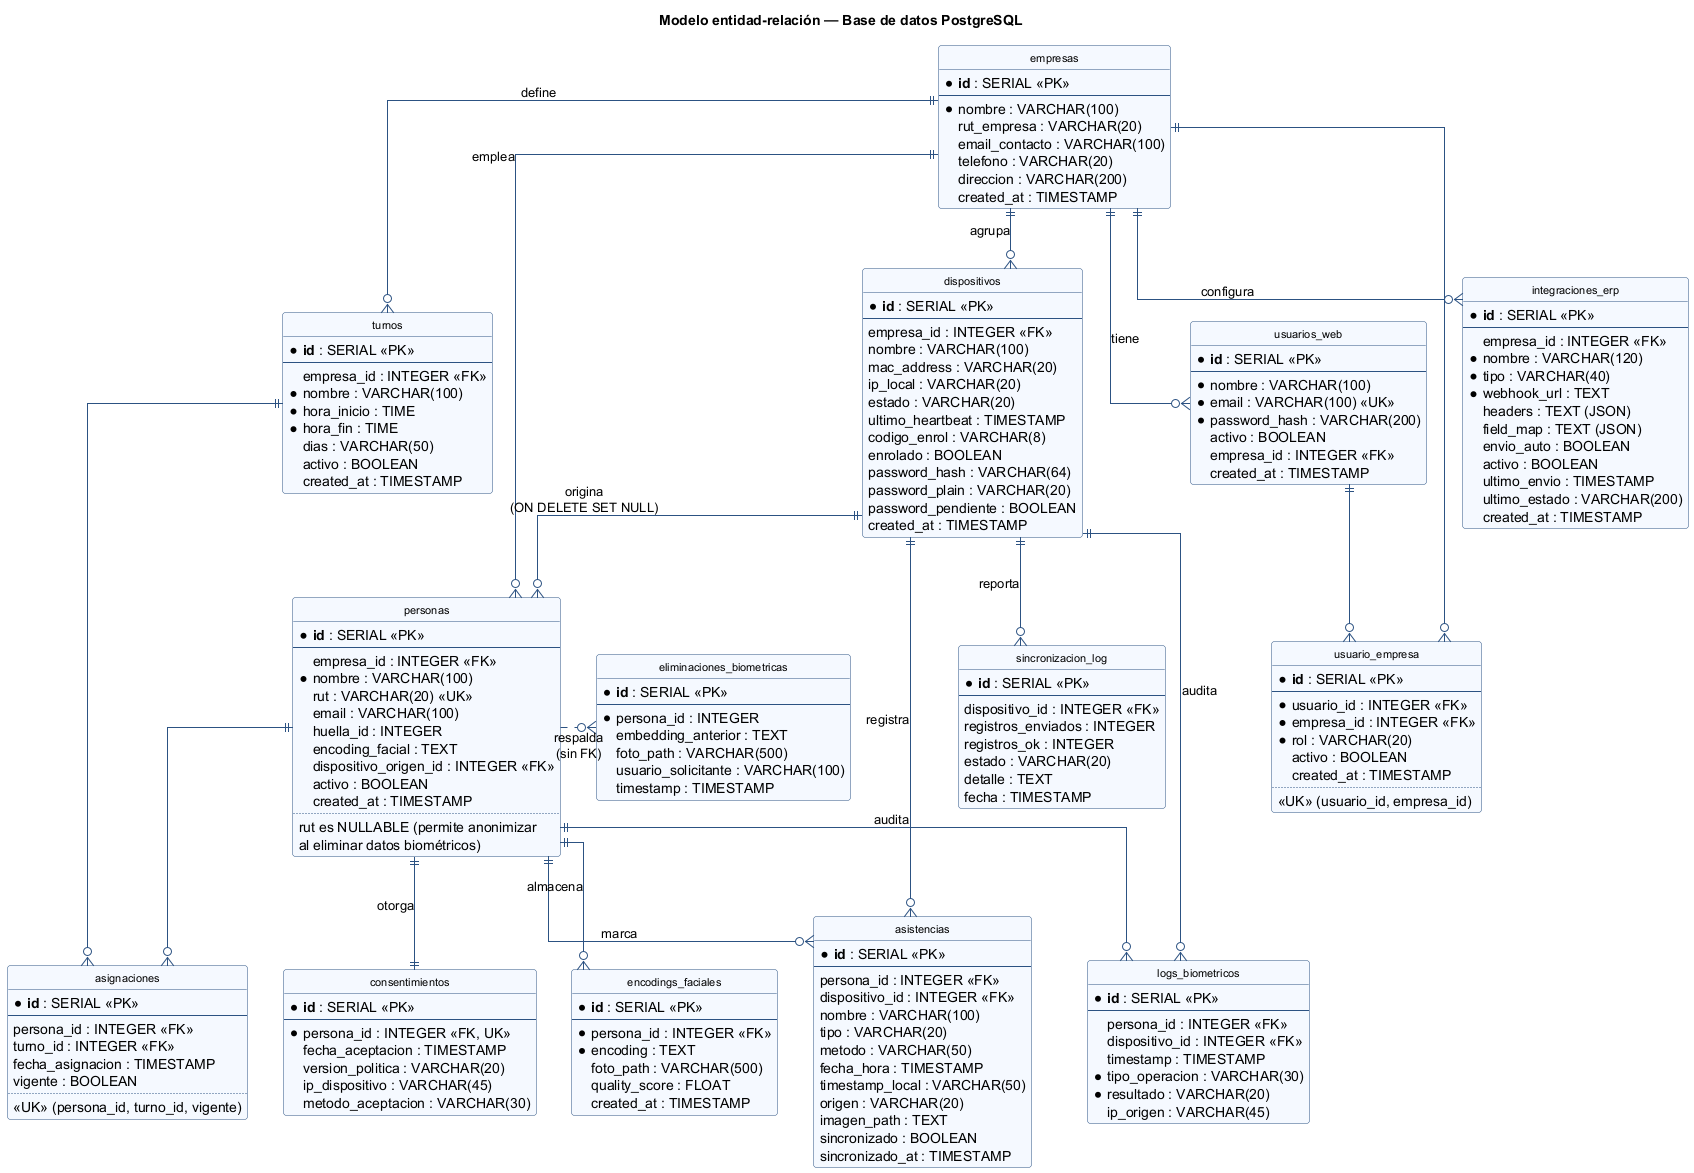
\includegraphics[width=\linewidth]{diagrams/diagrama_er_base_datos.png}
    \caption{Diagrama entidad-relación de la base de datos (14 tablas).}
    \label{fig:db-er}
\end{figure}

Las imágenes faciales, tanto las de registro como las de identificación durante la marcación, viajan del ESP32-CAM al backend por HTTP, como un JPEG crudo en formato application/octet-stream dirigido al endpoint correspondiente (POST /api/facial/registrar o POST /api/facial/identificar). El backend responde en la misma petición indicando si la foto fue aceptada, de modo que el dispositivo no necesita esperar un mensaje aparte para saber el resultado.

MQTT queda reservado para los eventos de estado del dispositivo, que son livianos y no requieren transportar una imagen. Se definen los tópicos esp32/heartbeat/<MAC> para monitorizar la actividad de los dispositivos y esp32/lwt/<MAC> para detectar desconexiones mediante el mecanismo de Last Will Testament (LWT). Para la detección activa de desconexión, se implementó el tópico esp32/ping/<MAC>: el backend publica un ping cada 30 segundos; si el ESP32-CAM no responde con un heartbeat dentro de 60 segundos, se marca como inactivo. La Figura~\ref{fig:flujo_mqtt} resume la topología de publicación y suscripción.

\begin{figure}[H]
  \centering
  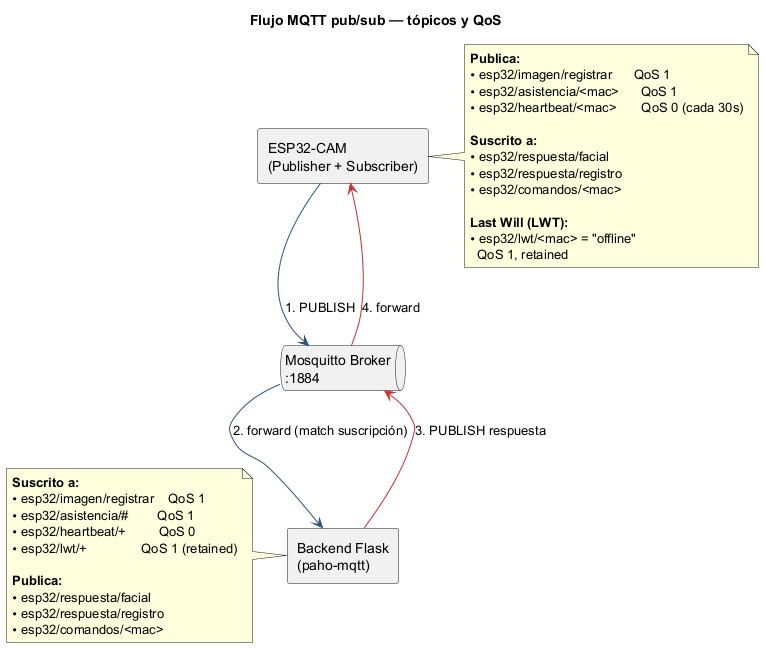
\includegraphics[width=\linewidth]{diagrams/flujo_mqtt_pub_sub.png}
  \caption{Flujo MQTT pub/sub: tópicos, direcciones y QoS entre el ESP32-CAM, el broker Mosquitto y el backend.}
  \label{fig:flujo_mqtt}
\end{figure}

\subsubsection{Implementación}

La implementación de la Iteración 3 se centró en habilitar la comunicación entre el dispositivo ESP32-CAM y el backend desarrollado en Python con Flask \cite{flask_docs}, así como en construir la base de datos PostgreSQL, accedida mediante el adaptador psycopg2 \cite{psycopg2_docs}, que soporta todo el sistema.

\paragraph{Inicialización de la base de datos}

Se implementó el módulo database.py con una función init\_db() que crea todas las tablas del sistema utilizando sentencias CREATE TABLE IF NOT EXISTS, asegurando idempotencia en los despliegues. Adicionalmente, se aplican sentencias ALTER TABLE ADD COLUMN IF NOT EXISTS para garantizar migraciones no destructivas. La función incluye la creación de índices sobre columnas frecuentemente consultadas (persona\_id, dispositivo\_id, fecha\_hora, empresa\_id) y la inserción de datos semilla (empresa por defecto, usuario administrador con contraseña hasheada).

\paragraph{Conexión Wi-Fi del ESP32-CAM y gestión de conectividad}

Para permitir la operación en red, el dispositivo implementa un mecanismo de conexión automática a Wi-Fi mediante la función tryConnectWiFi(). Esta función lee las credenciales desde wifi.json, configura el modo STA y deshabilita el ahorro de energía Wi-Fi (WIFI\_PS\_NONE) para mantener una conexión estable. La verificación continua de conectividad se realiza en verificarConexionWiFi(), que implementa un mecanismo de reintentos con backoff progresivo: tras detectar una desconexión, espera un tiempo creciente antes de reintentar (3s, 6s, 9s, 12s, 15s). Si tras 5 intentos fallidos no se logra reconectar, el dispositivo activa el Access Point como fallback.

El evento ARDUINO\_EVENT\_WIFI\_STA\_DISCONNECTED queda registrado con su código de razón y un contador de desconexiones, información expuesta a través del endpoint /wifi-diag para diagnóstico remoto.

\paragraph{Envío de imágenes faciales por HTTP: registro e identificación}

Tanto el registro como la identificación facial envían la imagen al backend de la misma manera: como JPEG crudo, sin codificarla en Base64, lo que evita el costo de procesamiento y el aumento de tamaño que implica esa codificación. Durante el registro, cuando el usuario presiona el botón de captura en la interfaz del dispositivo, el firmware toma la foto con la cámara en su calidad más alta y la sube de inmediato al backend mediante una petición POST, identificando a la persona con su RUT en una cabecera de la solicitud. El backend procesa la imagen y responde en esa misma petición si quedó aceptada o si hay que repetir la captura, lo que el dispositivo refleja en el contador de fotos de la pantalla de registro.

Durante la identificación (la consulta que ocurre al momento de marcar asistencia), el flujo es prácticamente el mismo a nivel de transporte: la imagen se captura y se envía por HTTP al endpoint de identificación, y el backend responde de forma síncrona indicando a qué persona corresponde el rostro, o un error si no encuentra coincidencia. Usar el mismo mecanismo síncrono para ambos casos simplificó el firmware, que ya no necesita dos rutas distintas para llegar al backend según el tipo de operación.

La Figura~\ref{fig:maquina_estados_esp32} ilustra la máquina de estados completa del proceso de enrolamiento biométrico en el ESP32-CAM, integrando la captura de huella digital (introducida en la Iteración 2) con el envío de la foto de referencia al backend por HTTP descrito en esta sección.

\begin{figure}[H]
  \centering
  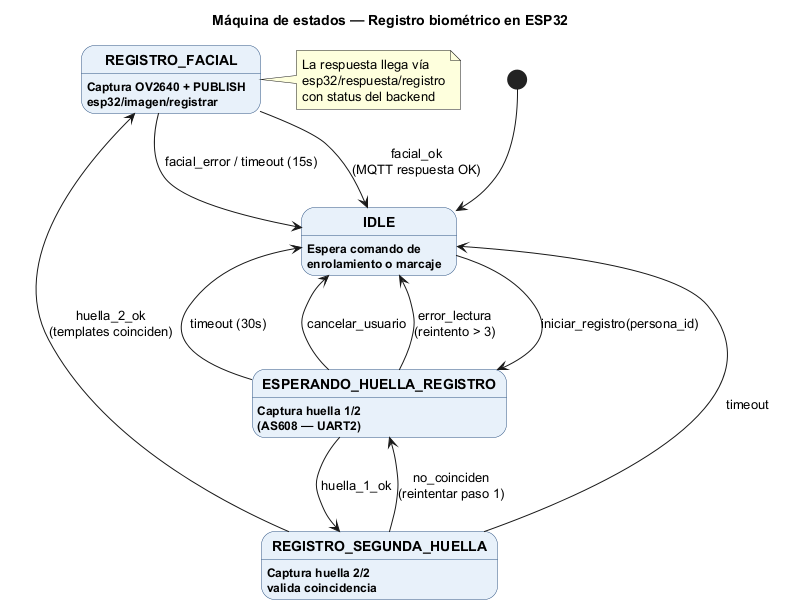
\includegraphics[width=\linewidth]{diagrams/maquina_estados_esp32.png}
  \caption{Máquina de estados del registro biométrico en el ESP32-CAM.}
  \label{fig:maquina_estados_esp32}
\end{figure}

\paragraph{Recepción de imágenes en el backend}

El backend recibe las fotos de registro e identificación a través de los endpoints REST del módulo routes/facial.py, descritos en el diseño de esta sección (ver Anexo B para el detalle completo de endpoints REST y tópicos MQTT). Al llegar una foto de registro, el backend verifica que exista consentimiento biométrico para esa persona, guarda la imagen, extrae el embedding facial y lo cifra antes de almacenarlo; si algo falla en el camino (consentimiento faltante, imagen borrosa, rostro duplicado), responde con el error correspondiente en lugar de dejar la solicitud sin respuesta.

Aparte de las imágenes, el backend mantiene un cliente MQTT para los eventos de estado del dispositivo: procesa los heartbeats, actualizando la IP y la actividad del dispositivo en la base de datos, y los mensajes de desconexión abrupta (LWT), marcándolo como inactivo. También corre en segundo plano una tarea que envía un ping cada 30 segundos a cada dispositivo enrolado, como verificación activa de que sigue en línea. Cada cambio de estado se transmite a los clientes web en tiempo real mediante streaming SSE, para que el panel se actualice sin que el administrador tenga que recargar la página.

\paragraph{Mantenimiento de la conexión MQTT en el ESP32-CAM}

El dispositivo mantiene, en paralelo a sus conexiones HTTP, un cliente MQTT que se conecta al broker si hay uno configurado y el dispositivo tiene red. Soporta URLs con esquema mqtt://, ws:// o wss:// (WebSockets seguros con TLS). Al conectarse, registra un mensaje de último aviso (LWT) para que el backend se entere si el dispositivo se cae de forma abrupta, y queda suscrito al tópico de ping para responder de inmediato cuando el backend pregunta si sigue activo. Este canal MQTT se usa únicamente para esta señalización de estado: ni el registro ni la identificación facial dependen de él.

\paragraph{Envío de datos mediante HTTP desde el ESP32-CAM}

Se implementó la capacidad del ESP32-CAM para comunicarse con la API REST del backend mediante solicitudes HTTP usando la librería HTTPClient. La función auxiliar beginHttp() configura cada petición con timeout de 10 segundos y el header X-Device-MAC para que el backend pueda identificar al dispositivo emisor. Esta función es utilizada por todos los handlers que requieren comunicación con el backend:

\begin{itemize}
    \item sincronizarPersonasDesdeBackend(): Descarga la lista completa de personas desde GET /api/personas y la persiste en personas.json.
    \item sincronizarTurnosDesdeBackend(): Descarga turnos desde GET /api/turnos.
    \item sincronizarAsignacionesDesdeBackend(): Descarga asignaciones desde GET /api/asignaciones.
    \item crearTurnoEnBackend(): Crea un turno en el backend vía POST /api/turnos.
    \item postAsistenciaEnBackend(): Envía una asistencia individual vía POST /api/asistencias.
    \item sincronizarAsistencias(): Envía un lote de asistencias pendientes vía POST /api/asistencias/sync.
\end{itemize}

\paragraph{Implementación de la API REST del backend}

El backend se implementó con Flask, organizando las rutas en blueprints independientes por dominio:
\begin{itemize}
    \item personas\_bp (routes/personas.py): CRUD de personas con validación de email, unicidad de RUT y manejo de empresa.
    \item turnos\_bp (routes/turnos.py): CRUD de turnos con filtro por empresa.
    \item asignaciones\_bp (routes/asignaciones.py): CRUD de asignaciones con verificación de pertenencia a empresa.
    \item asistencias\_bp (routes/asistencias.py): Registro de asistencias individuales y sincronización por lotes.
    \item facial\_bp (routes/facial.py): Endpoints de reconocimiento facial (registro, verificación, identificación 1:N).
    \item dispositivos\_bp (routes/dispositivos.py): Gestión y verificación de dispositivos.
    \item logs\_bp (routes/logs.py): Consulta de logs de sincronización.
    \item erp\_bp (routes/erp.py): CRUD de integraciones ERP y envío de datos.
    \item auth\_bp (routes/auth.py): Autenticación de usuarios del panel web.
\end{itemize}

Cada blueprint se registra en la aplicación Flask principal (app.py), junto con la configuración de CORS para permitir peticiones desde cualquier origen. El backend se ejecuta en el puerto 5000 con modo debug activado y recarga automática deshabilitada para evitar conflictos con el cliente MQTT.

\paragraph{Infraestructura con Docker Compose}

Para garantizar un entorno reproducible, se definió un archivo docker-compose.yml que levanta el broker Mosquitto (imagen eclipse-mosquitto:latest) con el puerto 1884 (externo, mapeado al 1883 interno) para MQTT nativo y el puerto 9001 para WebSockets expuestos, volúmenes para configuración, datos y logs persistentes, y una red bridge dedicada. El backend Flask y la base de datos PostgreSQL pueden ejecutarse en el host o en contenedores adicionales según la configuración de despliegue. La Figura~\ref{fig:docker_despliegue} presenta el diagrama de despliegue completo.

\begin{figure}[H]
  \centering
  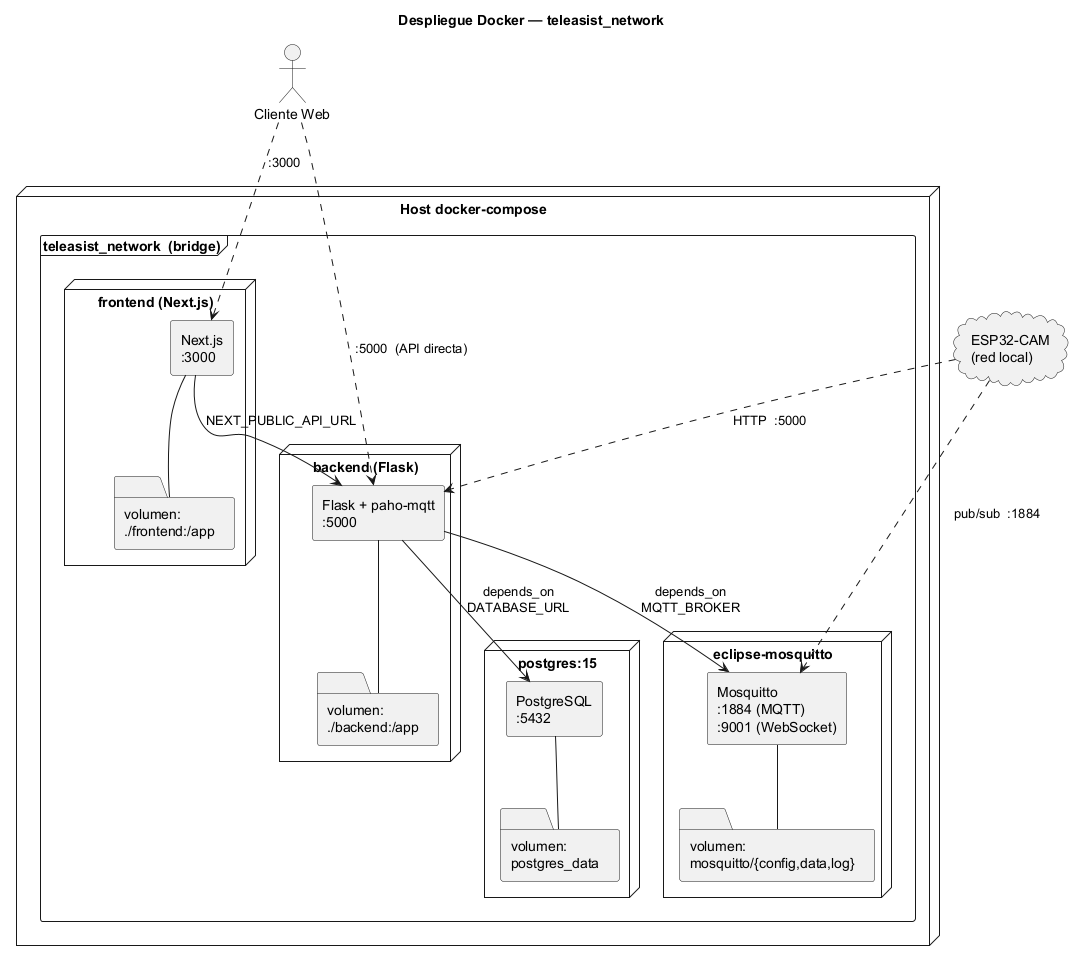
\includegraphics[width=\linewidth]{diagrams/arquitectura_despliegue_docker.png}
  \caption{Arquitectura de despliegue Docker: servicios, puertos, volúmenes y dependencias en la red.}
  \label{fig:docker_despliegue}
\end{figure}

\subsubsection{Pruebas}

Se diseñaron las siguientes pruebas para validar la comunicación y el backend:

\begin{itemize}
    \item \textbf{Prueba de conexión Wi-Fi y reconexión}: Configurar credenciales válidas en el ESP32-CAM, verificar que se conecte correctamente y obtenga una IP. Luego, apagar el router, verificar que el dispositivo detecte la desconexión mediante el evento de sistema y active el mecanismo de reintentos. Finalmente, encender el router y verificar que el dispositivo reconecte automáticamente en menos de 30 segundos.

    \item \textbf{Prueba de envío de imagen facial por HTTP}: Capturar una imagen desde el ESP32-CAM y enviarla al endpoint de registro mediante POST. Verificar que el backend reciba la imagen, la guarde en disco y responda en la misma petición indicando si la foto fue aceptada.

    \item \textbf{Prueba de heartbeat y LWT}: Verificar que, estando el ESP32-CAM conectado, el backend reciba heartbeats periódicos (cada 30 segundos) y actualice el campo ultimo\_heartbeat en la tabla dispositivos. Desconectar el dispositivo abruptamente y verificar que el mensaje LWT se publique y el backend marque el dispositivo como inactivo en menos de 10 segundos.

    \item \textbf{Prueba de ping/pong activo}: Conectar el ESP32-CAM al broker MQTT. Verificar que el backend publique esp32/ping/<MAC> periódicamente (cada 30 segundos) y que el ESP32-CAM responda con un heartbeat que contenga el campo "pong": true. Detener la conectividad del ESP32-CAM y verificar que, tras 60 segundos sin respuesta, el backend marque el dispositivo como inactivo.

    \item \textbf{Prueba de recepción de datos en backend vía HTTP}: Enviar solicitudes POST a /api/personas, /api/turnos, /api/asignaciones y /api/asistencias desde el ESP32-CAM. Verificar que cada solicitud sea procesada correctamente por el backend (código HTTP 200/201) y que los datos queden persistidos en PostgreSQL.

    \item \textbf{Prueba de sincronización por lotes}: Generar 5 marcaciones offline en el ESP32-CAM, conectar el dispositivo a la red y ejecutar la sincronización. Verificar que los 5 registros lleguen al backend vía POST /api/asistencias/sync, que se inserten correctamente y que el dispositivo marque cada registro como sincronizado = true.

    \item \textbf{Prueba de inicialización de base de datos}: Ejecutar init\_db() sobre una base de datos vacía. Verificar que se creen las 14 tablas, los índices y los datos semilla (empresa por defecto y usuario administrador) sin errores.

    \item \textbf{Prueba de latencia de transmisión}: Medir el tiempo total desde que el ESP32-CAM envía una imagen por HTTP hasta que recibe la respuesta de confirmación del backend. Se espera un tiempo menor a 5 segundos en condiciones de red local.
\end{itemize}

\paragraph{Nuevos tópicos MQTT para control y notificación}

En iteraciones posteriores se agregaron los siguientes tópicos al ecosistema MQTT:

\begin{itemize}
    \item backend/comando/<MAC>: Permite al backend enviar comandos remotos al ESP32-CAM. La función enviar\_comando\_dispositivo() en mqtt\_handler.py publica un JSON con el campo comando en este tópico.

    \item backend/notificacion/<MAC>: Utilizado por el módulo eventos\_mqtt.py para notificar a los dispositivos que deben sincronizar sus datos. Cada vez que se crea, actualiza o elimina una persona, turno o asignación, la función notificar\_sincronizacion() publica un mensaje indicando el tipo de entidad y la acción realizada.

    \item esp32/huella/resultado/<huella\_id>: Tópico en el que el ESP32-CAM publica el resultado del enrolamiento de una huella. El backend se suscribe a esp32/huella/resultado/\# y procesa la respuesta, actualizando la persona correspondiente y notificando a través de SSE.
\end{itemize}

\paragraph{Módulo eventos\_mqtt.py}

Se implementó el módulo eventos\_mqtt.py con la función notificar\_sincronizacion(empresa\_id, tipo, accion, registro\_id). Esta función consulta los dispositivos enrolados de la empresa y publica un mensaje en backend/notificacion/<MAC> por cada uno, permitiendo que los ESP32-CAM reciban notificaciones en tiempo real sobre cambios en personas, turnos y asignaciones. Es invocada desde routes/personas.py, routes/turnos.py y routes/asignaciones.py tras cada operación de creación, actualización o eliminación.

\paragraph{Streaming SSE de huellas}

Para mantener actualizados los clientes web durante el enrolamiento de huellas, se implementó el endpoint GET /sse/huellas en app.py. La función broadcast\_huella\_update() difunde los resultados del enrolamiento (recibidos por MQTT en esp32/huella/resultado/\#) a todos los clientes conectados al SSE, permitiendo que el panel web muestre en tiempo real el progreso del registro biométrico.

\subsubsection{Refinamientos posteriores}

\begin{itemize}
    \item \textbf{Decorador @requiere\_dispositivo\_enrolado}: definido en routes/auth.py, valida que el dispositivo asociado a la petición (request.dispositivo\_id) exista en la tabla dispositivos con enrolado = TRUE, devolviendo 403 en caso contrario. Se aplica sobre endpoints biométricos sensibles como /api/facial/registrar, evitando que un dispositivo no autorizado opere sobre datos biométricos.

    \item \textbf{Integridad referencial con ON DELETE SET NULL y RUT nullable}: la columna dispositivo\_origen\_id de la tabla personas (y dispositivo\_id de asistencias) se definió con REFERENCES dispositivos(id) ON DELETE SET NULL, de modo que eliminar un dispositivo no elimina en cascada las personas ni asistencias asociadas, sino que conserva el historial con la referencia en NULL. De forma análoga, la columna rut de personas se migró a nullable (ALTER TABLE personas ALTER COLUMN rut DROP NOT NULL) para permitir el borrado de datos sensibles de una persona sin perder su historial de asistencias.
\end{itemize}


%% ============================================================
%% ITERACIÓN 4: Reconocimiento facial, anti-spoofing y cifrado
%% ============================================================

\subsection{Iteración 4: Reconocimiento facial, anti-spoofing y cifrado biométrico}

Esta iteración incorpora el procesamiento biométrico en el backend: reconocimiento facial con DeepFace, validación anti-spoofing y cifrado de embeddings faciales. El sistema pasa de solo transmitir imágenes a realizar verificación e identificación biométrica.

\subsubsection{Análisis}

Para incorporar el reconocimiento facial al sistema, se evaluaron diversas librerías y modelos de deep learning. Se seleccionó DeepFace por las siguientes razones:

\begin{itemize}
    \item Soporta múltiples modelos de reconocimiento facial (Facenet, VGG-Face, ArcFace, etc.) y detectores (RetinaFace, MTCNN, OpenCV, etc.).
    \item Incluye funcionalidad de anti-spoofing integrada, capaz de distinguir entre un rostro real y una fotografía o pantalla, analizando textura, profundidad y reflectancia de la piel.
    \item Su API en Python es sencilla de integrar con Flask y compatible con las imágenes JPEG capturadas por la cámara OV2640 del ESP32-CAM.
    \item Facenet genera embeddings de 128 dimensiones, optimizando el almacenamiento y la velocidad de comparación.
\end{itemize}

Se identificaron los siguientes requisitos funcionales para esta iteración:

\begin{itemize}
    \item \textbf{Registro facial}: Recibir una imagen del ESP32-CAM, extraer el embedding facial, validar que el rostro no esté duplicado en la base de datos (detección de identidades repetidas) y almacenar el embedding cifrado.
    \item \textbf{Identificación 1:N}: Dada una imagen capturada en vivo, comparar su embedding contra todos los embeddings almacenados y retornar la identidad con mayor coincidencia, si supera el umbral de similitud.
    \item \textbf{Verificación 1:1}: Dada una imagen y un rut, verificar si la imagen corresponde a la persona declarada.
    \item \textbf{Anti-spoofing}: Detectar intentos de suplantación mediante fotografías impresas, pantallas de dispositivos o máscaras, rechazando la captura si no se detecta un rostro real.
    \item \textbf{Cifrado de embeddings}: Los vectores de características faciales (embeddings) son datos biométricos sensibles. Para protegerlos, se deben cifrar antes de persistirlos en la base de datos, utilizando una clave derivada de una variable de entorno.
    \item \textbf{Consentimiento biométrico}: Todo registro facial debe estar precedido por la aceptación explícita de una política de privacidad por parte del trabajador, en cumplimiento de la normativa de protección de datos.
\end{itemize}

\subsubsection{Diseño}

El flujo de procesamiento facial se divide en tres operaciones principales:

\begin{enumerate}
    \item \textbf{Registro} (POST /api/facial/registrar):
    \begin{itemize}
        \item Recibe la imagen como JPEG crudo (application/octet-stream) con el RUT en un header HTTP, que es como la envía el dispositivo, o como JSON con la imagen en Base64, opción que se mantiene para clientes web.
        \item Verifica que exista consentimiento biométrico en la tabla consentimientos. Si no existe, rechaza con HTTP 403.
        \item Guarda la imagen como static/previews/<id>.jpg.
        \item Aplica un \textbf{filtro de calidad de imagen} que mide la nitidez mediante la varianza del Laplaciano \cite{pech2000_laplacian}. Si la imagen es demasiado plana o borrosa (por debajo de un umbral configurable, 50 por defecto), se rechaza como posible intento de suplantación (foto de pantalla o papel) antes de llegar a DeepFace, ahorrando procesamiento innecesario del modelo.
        \item Extrae el embedding con DeepFace usando el modelo Facenet y un detector configurable mediante variable de entorno (FACIAL\_DETECTOR), utilizando MTCNN por defecto por su velocidad (tres veces más rápido que RetinaFace con precisión comparable) y sin anti-spoofing en esta etapa.
        \item Cifra el embedding con Fernet y lo almacena en la tabla encodings\_faciales, que permite acumular múltiples fotos de referencia por persona con distintos ángulos e iluminación, mejorando la precisión en subsecuentes identificaciones.
    \end{itemize}

    El flujo completo de enrolamiento biométrico, desde la creación de la persona en el panel web por parte del administrador, pasando por el registro de huella en dos pasos en el ESP32-CAM, hasta la captura facial enviada por HTTP al backend donde se extrae, cifra y almacena el embedding, se ilustra en el diagrama de secuencia de la Figura~\ref{fig:flujo_enrolamiento} del Anexo C.

    \item \textbf{Identificación 1:N} (POST /api/facial/identificar):
    \begin{itemize}
        \item Recibe la imagen como JPEG crudo (application/octet-stream) desde el ESP32-CAM, o como JSON con Base64 desde la web.
        \item Aplica el mismo filtro de calidad Laplacian como barrera anti-spoofing previa, rechazando imágenes de baja nitidez antes de invocar DeepFace.
        \item Extrae el embedding con DeepFace (anti-spoofing activado mediante anti\_spoofing=True).
        \item Consulta una caché en memoria de embeddings (con TTL configurable, 60 segundos por defecto). Si la caché expiró, recarga todos los embeddings desde la base de datos. Para cada persona, compara contra todos los embeddings almacenados en encodings\_faciales (multi-encoding) y selecciona la menor distancia. Esto mejora la precisión porque el sistema puede reconocer a un trabajador aunque la captura en vivo tenga una iluminación o ángulo diferentes a los de su foto de registro.
        \item Si la menor distancia es inferior al umbral (10.0 para Facenet), retorna el rut correspondiente. En caso contrario, retorna HTTP 404.
    \end{itemize}

    El ciclo de marcaje automático por centinela facial, en el que cada 6 segundos el ESP32-CAM evalúa el sensor PIR, captura una imagen, la envía por HTTP al endpoint de identificación, y según la respuesta del backend registra la asistencia y dispara el push asíncrono a los ERP configurados, se presenta en el diagrama de secuencia de la Figura~\ref{fig:flujo_marcaje} del Anexo C, dado su tamaño.

    \item \textbf{Verificación 1:1} (POST /api/facial/verificar):
    \begin{itemize}
        \item Recibe rut e imagen (Base64).
        \item Descifra todos los embeddings almacenados para esa persona en encodings\_faciales y extrae el embedding de la imagen capturada (con anti-spoofing activado).
        \item Calcula la distancia euclidiana contra cada embedding de referencia y selecciona la menor. Si es menor que 10.0, retorna éxito con el nivel de confianza calculado como max(0, (1 - distancia/20) * 100).
    \end{itemize}
\end{enumerate}

El modelo seleccionado es Facenet por su equilibrio entre precisión y tamaño de embedding (128 dimensiones). El detector facial es configurable mediante variable de entorno (FACIAL\_DETECTOR), utilizando MTCNN por defecto. Si bien RetinaFace ofrece mayor robustez ante variaciones extremas de pose e iluminación, MTCNN es tres veces más rápido y mantiene una precisión comparable para las condiciones típicas de una cámara de control de asistencia (rostro frontal a corta distancia), lo que lo hace más adecuado para un dispositivo embebido como el ESP32-CAM. El umbral de 10.0 para la distancia euclidiana fue elegido con base en la documentación de DeepFace y ajustes empíricos realizados durante el desarrollo.

Para el cifrado de embeddings se utiliza el algoritmo Fernet (AES-128 en modo CBC con HMAC-SHA256 para autenticación), parte de la librería cryptography de Python. La clave de cifrado se deriva aplicando SHA-256 a una variable de entorno (BIOMETRIC\_KEY), garantizando que los embeddings nunca se almacenen en texto plano en la base de datos.

\subsubsection{Implementación}

\paragraph{Procesamiento de imágenes en el backend}

El módulo routes/facial.py implementa los tres endpoints descritos en el diseño. Las funciones auxiliares incluyen:

\begin{itemize}
    \item \_validar\_calidad\_imagen(img\_path): Aplica el filtro Laplaciano (varianza del Laplaciano) sobre la imagen decodificada para medir su nitidez. Si el valor está por debajo del umbral configurable en FACIAL\_NITIDEZ\_UMBRAL (50 por defecto), la imagen se considera borrosa o plana (posible foto de pantalla o papel) y se rechaza antes de llegar a DeepFace, funcionando como una capa adicional de anti-spoofing.
    \item extraer\_embedding(img\_path, anti\_spoofing): Invoca DeepFace.represent() con el modelo Facenet pre-cargado y el detector configurable vía variable de entorno. Si anti\_spoofing=True, activa la detección de suplantación.
    \item guardar\_imagen\_de\_registro(persona\_id, imagen\_b64): Decodifica la imagen Base64, la convierte a RGB con Pillow y la guarda en static/previews/<id>.jpg.
    \item \_verificar\_consentimiento(persona\_id): Consulta la tabla consentimientos para verificar que exista un registro de aceptación.
    \item \_log\_biometrico(persona\_id, dispositivo\_id, tipo\_operacion, resultado): Inserta un registro de auditoría en logs\_biometricos.
\end{itemize}

Además, para optimizar el rendimiento, el modelo Facenet se precarga al iniciar el servidor mediante DeepFace.build\_model('Facenet', task='facial\_recognition'), eliminando la latencia de carga de pesos en la primera solicitud. Los embeddings almacenados en la base de datos se mantienen en una caché en memoria con tiempo de vida configurable (por defecto 60 segundos, mediante FACIAL\_CACHE\_TTL), evitando consultas repetitivas y descifrados a la base de datos en cada identificación. La caché se invalida automáticamente al registrar una nueva foto o al eliminar datos biométricos, garantizando consistencia.

\paragraph{Cifrado y descifrado de embeddings}

El módulo encryption.py proporciona dos funciones:

\begin{itemize}
    \item cifrar\_embedding(embedding): Serializa el embedding como JSON, lo cifra con Fernet y codifica el resultado en Base64 URL-safe.
    \item descifrar\_embedding(cifrado\_str): Decodifica el Base64, descifra con Fernet y deserializa el JSON para obtener el vector original.
\end{itemize}

% =====================================================================
% Diagrama 8 — Pipeline de cifrado biométrico (TikZ)
% Incluir en memoria.tex con:  % =====================================================================
% Diagrama 8 — Pipeline de cifrado biométrico (TikZ)
% Incluir en memoria.tex con:  \input{diagrams/08_pipeline_cifrado_biometrico.tex}
% Requiere en el preámbulo: \usepackage{tikz}
%                           \usetikzlibrary{arrows.meta, positioning, shapes.geometric}
% =====================================================================
\begin{figure}[H]
\centering
\begin{tikzpicture}[
  node distance=1.1cm and 1.3cm,
  every node/.style={font=\small},
  box/.style={draw, rounded corners=3pt, minimum height=1.1cm,
              minimum width=2.7cm, align=center, fill=blue!8,
              drop shadow={opacity=0.15}},
  crypto/.style={draw, rounded corners=3pt, minimum height=1.1cm,
                 minimum width=2.7cm, align=center, fill=orange!20,
                 drop shadow={opacity=0.15}},
  db/.style={draw, cylinder, shape border rotate=90, aspect=0.25,
             minimum height=1.5cm, minimum width=2.5cm,
             align=center, fill=gray!15},
  fallback/.style={draw, dashed, rounded corners=3pt, minimum height=1.0cm,
                   minimum width=2.7cm, align=center, fill=red!8},
  arrow/.style={-{Stealth[length=2.5mm]}, thick},
  darrow/.style={-{Stealth[length=2.5mm]}, thick, dashed, gray!70!black},
  lbl/.style={font=\scriptsize\itshape, text=gray!50!black}
]

% --- Fila superior: cifrado ---
\node[box]                       (emb)    {Embedding\\\scriptsize{\texttt{float[512]}}};
\node[crypto, right=of emb]      (cif)    {\texttt{cifrar\_embedding()}};
\node[crypto, right=of cif]      (fernet) {Fernet\\\scriptsize{AES-128-CBC + HMAC-SHA256}};
\node[db,     right=of fernet]   (dbn)    {PostgreSQL\\\scriptsize{TEXT (base64)}};

% --- Fila inferior: descifrado ---
\node[crypto, below=1.7cm of fernet] (dcif)    {\texttt{descifrar\_embedding()}};
\node[box,    left=of dcif]          (compare) {Comparación\\\scriptsize{DeepFace.verify}};

% --- Fallback ---
\node[fallback, below=0.7cm of dbn] (legacy) {Fallback legacy\\\scriptsize{embedding sin cifrar}};

% --- Flechas principales ---
\draw[arrow] (emb)    -- (cif);
\draw[arrow] (cif)    -- (fernet);
\draw[arrow] (fernet) -- (dbn);
\draw[arrow] (dbn)    |- (dcif);
\draw[arrow] (dcif)   -- (compare);

% --- Camino fallback ---
\draw[darrow] (legacy.west) -| ([xshift=-0.3cm]dcif.south)
              node[pos=0.75, below, font=\scriptsize] {parse directo};

% --- Etiquetas ---
\node[lbl, above=0.1cm of cif] {clave Fernet (\texttt{.env})};
\node[lbl, above=0.1cm of dcif] {misma clave (rotable)};

\end{tikzpicture}
\caption[Pipeline de cifrado biométrico]{Pipeline de cifrado biométrico — Fernet (AES-128-CBC + HMAC-SHA256) con fallback para embeddings legacy almacenados sin cifrar.}
\label{fig:pipeline_cifrado_biometrico}
\end{figure}

% Requiere en el preámbulo: \usepackage{tikz}
%                           \usetikzlibrary{arrows.meta, positioning, shapes.geometric}
% =====================================================================
\begin{figure}[H]
\centering
\begin{tikzpicture}[
  node distance=1.1cm and 1.3cm,
  every node/.style={font=\small},
  box/.style={draw, rounded corners=3pt, minimum height=1.1cm,
              minimum width=2.7cm, align=center, fill=blue!8,
              drop shadow={opacity=0.15}},
  crypto/.style={draw, rounded corners=3pt, minimum height=1.1cm,
                 minimum width=2.7cm, align=center, fill=orange!20,
                 drop shadow={opacity=0.15}},
  db/.style={draw, cylinder, shape border rotate=90, aspect=0.25,
             minimum height=1.5cm, minimum width=2.5cm,
             align=center, fill=gray!15},
  fallback/.style={draw, dashed, rounded corners=3pt, minimum height=1.0cm,
                   minimum width=2.7cm, align=center, fill=red!8},
  arrow/.style={-{Stealth[length=2.5mm]}, thick},
  darrow/.style={-{Stealth[length=2.5mm]}, thick, dashed, gray!70!black},
  lbl/.style={font=\scriptsize\itshape, text=gray!50!black}
]

% --- Fila superior: cifrado ---
\node[box]                       (emb)    {Embedding\\\scriptsize{\texttt{float[512]}}};
\node[crypto, right=of emb]      (cif)    {\texttt{cifrar\_embedding()}};
\node[crypto, right=of cif]      (fernet) {Fernet\\\scriptsize{AES-128-CBC + HMAC-SHA256}};
\node[db,     right=of fernet]   (dbn)    {PostgreSQL\\\scriptsize{TEXT (base64)}};

% --- Fila inferior: descifrado ---
\node[crypto, below=1.7cm of fernet] (dcif)    {\texttt{descifrar\_embedding()}};
\node[box,    left=of dcif]          (compare) {Comparación\\\scriptsize{DeepFace.verify}};

% --- Fallback ---
\node[fallback, below=0.7cm of dbn] (legacy) {Fallback legacy\\\scriptsize{embedding sin cifrar}};

% --- Flechas principales ---
\draw[arrow] (emb)    -- (cif);
\draw[arrow] (cif)    -- (fernet);
\draw[arrow] (fernet) -- (dbn);
\draw[arrow] (dbn)    |- (dcif);
\draw[arrow] (dcif)   -- (compare);

% --- Camino fallback ---
\draw[darrow] (legacy.west) -| ([xshift=-0.3cm]dcif.south)
              node[pos=0.75, below, font=\scriptsize] {parse directo};

% --- Etiquetas ---
\node[lbl, above=0.1cm of cif] {clave Fernet (\texttt{.env})};
\node[lbl, above=0.1cm of dcif] {misma clave (rotable)};

\end{tikzpicture}
\caption[Pipeline de cifrado biométrico]{Pipeline de cifrado biométrico — Fernet (AES-128-CBC + HMAC-SHA256) con fallback para embeddings legacy almacenados sin cifrar.}
\label{fig:pipeline_cifrado_biometrico}
\end{figure}


\paragraph{Actualización y eliminación de datos faciales}

Se implementó el endpoint PUT /api/facial/actualizar/<persona\_id> que permite reemplazar el embedding y la foto de una persona existente. También se implementó DELETE /api/personas/<id>/datos-biometricos que elimina el embedding facial, la huella asociada, la foto en disco y el consentimiento, pero conserva los registros de asistencia históricos. La eliminación queda registrada en la tabla eliminaciones\_biometricas para trazabilidad.

Se implementó además el endpoint POST /api/facial/agregar-foto que permite agregar fotos de referencia adicionales a una persona ya registrada, sin reemplazar las existentes. Cada nueva foto pasa por el mismo filtro de calidad Laplacian y se almacena como un nuevo registro en encodings\_faciales. Esta funcionalidad de enrolamiento progresivo permite mejorar la precisión del sistema a lo largo del tiempo: si un trabajador experimenta falsos rechazos, se le pueden agregar más fotos de referencia con distintos ángulos o condiciones de iluminación, aumentando la robustez del reconocimiento sin necesidad de rehacer el registro completo.

\subsubsection{Pruebas}

Se diseñaron las siguientes pruebas para validar el módulo de reconocimiento facial:

\begin{itemize}
    \item \textbf{Prueba de registro facial exitoso}: Enviar una imagen facial válida junto con un rut que tenga consentimiento registrado. Verificar que el backend extraiga el embedding, lo almacene cifrado y responda con HTTP 200.

    \item \textbf{Prueba de detección de duplicados}: Registrar una segunda imagen del mismo rostro para otra persona. Verificar que el backend detecte la similitud (distancia < 10.0) y rechace el registro con HTTP 409, indicando el nombre de la persona con la que coincide.

    \item \textbf{Prueba de rechazo por falta de consentimiento}: Intentar registrar un rostro para una persona sin consentimiento biométrico. Verificar que el backend rechace la operación con HTTP 403.

    \item \textbf{Prueba de identificación 1:N}: Registrar 3 personas con sus respectivas fotos. Enviar una nueva foto de una de ellas al endpoint de identificación. Verificar que el backend retorne el rut correcto.

    \item \textbf{Prueba de identificación con rostro desconocido}: Enviar una foto de una persona no registrada. Verificar que el backend retorne HTTP 404 y registre el intento fallido en logs\_biometricos.

    \item \textbf{Prueba de anti-spoofing con fotografía impresa}: Capturar una foto de un rostro registrado desde una pantalla o impresión y enviarla al endpoint de identificación. Verificar que DeepFace con anti\_spoofing=True rechace la imagen por no detectar un rostro real (excepción ValueError con mensaje ``Spoof detected'').

    \item \textbf{Prueba de resistencia a condiciones de iluminación}: Capturar imágenes del mismo rostro bajo 3 condiciones de iluminación (luz natural, luz artificial tenue, contraluz). Verificar que los 3 embeddings generados mantengan distancia euclidiana entre sí menor a 10.0 y que el sistema identifique correctamente a la persona.

    \item \textbf{Prueba de cifrado y descifrado}: Almacenar un embedding en la base de datos y verificar que el valor en la columna encoding\_facial no sea legible (no contenga los números del vector en texto plano). Luego, recuperar el registro y descifrar el embedding; verificar que el vector original se reconstruya idénticamente.

    \item \textbf{Prueba de eliminación de datos biométricos}: Ejecutar el endpoint de eliminación de datos biométricos para una persona con rostro registrado. Verificar que el embedding se elimine de la base de datos, que la foto se borre del disco, que el consentimiento se elimine, que los registros de asistencia se conserven y que quede una entrada en eliminaciones\_biometricas.

    \item \textbf{Prueba de filtro de calidad de imagen}: Enviar al endpoint de registro una imagen deliberadamente borrosa o una foto de una pantalla (baja varianza de Laplacian). Verificar que el backend rechace la imagen antes de invocar DeepFace, retornando un error de calidad insuficiente.

    \item \textbf{Prueba de múltiples fotos de referencia}: Registrar una persona con una foto frontal. Luego, agregar una segunda foto de la misma persona con distinto ángulo mediante POST /api/facial/agregar-foto. Realizar una identificación con una tercera foto y verificar que el sistema reconozca a la persona correctamente, comparando contra ambos embeddings de referencia.
    
    \item \textbf{Prueba de caché de embeddings}: Realizar una identificación exitosa y verificar los tiempos de respuesta. Realizar una segunda identificación inmediatamente después; verificar que el tiempo sea significativamente menor porque los embeddings se sirvieron desde la caché en memoria sin consultar la base de datos.
\end{itemize}

\paragraph{Endpoint identificar-o-registrar}

Se implementó el endpoint POST /api/facial/identificar-o-registrar que combina ambos flujos en una sola llamada: primero intenta identificar a la persona por su rostro; si la identificación es exitosa, retorna los datos de la persona; si falla y se proporciona un RUT con consentimiento biométrico, registra automáticamente la nueva persona con el embedding facial extraído. Este endpoint facilita el enrolamiento progresivo en el dispositivo: un trabajador puede colocarse frente al ESP32-CAM y, si ya está registrado, se marca su asistencia; si no, el sistema lo registra sobre la marcha. El endpoint incluye validación de calidad de imagen, anti-spoofing y log biométrico tanto para identificación como para registro.

\subsubsection{Refinamientos posteriores}

\begin{itemize}
    \item \textbf{Transmisión de imágenes vía octet-stream}: el envío de la imagen facial migró de un esquema basado en JSON con la foto codificada en Base64 a un envío binario directo (Content-Type: application/octet-stream) con el RUT o la MAC del dispositivo en un header HTTP (X-RUT / X-Device-MAC). El backend mantiene compatibilidad retroactiva con el formato Base64 como \textit{fallback}. El cambio elimina el overhead de codificación Base64 (aproximadamente 33\% de tamaño adicional) y simplifica el firmware, que ahora envía directamente el buffer JPEG capturado por la cámara (fb->buf, fb->len).

    \item \textbf{Captura de 3 fotos de referencia por persona}: el flujo de registro se extendió de una sola foto a tres capturas sucesivas (FOTOS\_REQUERIDAS = 3 en el firmware), idealmente frontal y de ambos perfiles, generando tres embeddings independientes almacenados en la tabla encodings\_faciales. Esto mejora la tasa de identificación ante variaciones de ángulo o iluminación, ya que la comparación 1:N evalúa contra todos los embeddings de referencia disponibles.
\end{itemize}


%% ============================================================
%% ITERACIÓN 5: Autenticación, multi-tenant y enrolamiento
%% ============================================================

\subsection{Iteración 5: Autenticación, multi-tenant y enrolamiento de dispositivos}

La quinta iteración incorpora la capa de seguridad y administración del sistema: autenticación de usuarios del panel web mediante JWT, un modelo multi-tenant que permite a múltiples empresas operar sobre la misma instancia del backend con datos aislados, y un mecanismo seguro de enrolamiento de dispositivos ESP32-CAM mediante PIN de un solo uso.

\subsubsection{Análisis}

El sistema, al estar orientado a un entorno empresarial, requiere que diferentes organizaciones puedan utilizar la misma plataforma sin que sus datos se mezclen. Asimismo, el panel web administrativo debe restringir el acceso según el rol del usuario. Finalmente, cada dispositivo ESP32-CAM debe ser vinculado de forma segura a una empresa específica, evitando que dispositivos no autorizados inyecten datos en el sistema.

Los requisitos identificados son:

\begin{itemize}
    \item \textbf{Multi-tenant}: Cada entidad (persona, turno, asignación, asistencia, dispositivo) debe pertenecer a una empresa. Las consultas deben filtrarse por empresa según el contexto del usuario autenticado. El administrador global (rol admin) tiene visibilidad sobre todas las empresas.
    \item \textbf{Autenticación JWT}: El panel web backend debe requerir autenticación para operaciones sensibles. Los tokens JWT (JSON Web Tokens), firmados con HMAC-SHA256, transportan el ID de usuario, la empresa seleccionada y su rol. Tienen expiración de 24 horas.
    \item \textbf{Roles de usuario}: Se definen tres roles jerárquicos:
    \begin{itemize}
        \item admin: Acceso total al sistema, puede crear empresas, gestionar todos los usuarios y dispositivos.
        \item empleador: Acceso limitado a los datos de su empresa; puede gestionar trabajadores, turnos y ver asistencias.
        \item trabajador: Acceso restringido a sus propios datos de asistencia.
    \end{itemize}
    \item \textbf{Enrolamiento de dispositivos}: Un administrador genera un PIN de 8 caracteres en el panel web. Ese PIN se ingresa en el ESP32-CAM (vía web embebida), que lo envía al backend junto con su MAC address. Si el PIN es válido y no ha sido usado, el dispositivo queda enrolado y asociado a la empresa correspondiente.
    \item \textbf{Auto-registro de empresas}: Se requiere un endpoint público que permita a una nueva organización registrarse de forma autónoma en el sistema, sin intervención del administrador central. La empresa proporciona sus datos (nombre, RUT, email, etc.) y los datos del usuario administrador; el sistema crea la empresa, el usuario, y la asociación entre ambos con rol admin en una sola transacción atómica, retornando un token JWT para que el nuevo administrador quede autenticado inmediatamente. Esto facilita el despliegue del sistema en nuevos clientes sin requerir configuración manual previa.
    \item \textbf{Monitorización de dispositivos}: Una vez enrolado, el ESP32-CAM envía heartbeats periódicos vía MQTT. El backend actualiza el estado del dispositivo (activo) y registra su última actividad. Un proceso watchdog marca como inactivo a los dispositivos que no han enviado heartbeat en más de 90 segundos.
\end{itemize}

\subsubsection{Diseño}

\paragraph{Modelo de datos multi-tenant}

La estrategia multi-tenant se implementa a nivel de base de datos mediante una columna empresa\_id en las tablas personas, turnos, dispositivos, integraciones\_erp y asistencias (esta última a través de la relación con personas). La tabla empresas actúa como entidad raíz del tenant. La tabla asociativa usuario\_empresa vincula usuarios con empresas y define el rol que cada usuario tiene en cada empresa, permitiendo que un mismo usuario tenga roles distintos en diferentes organizaciones.

\paragraph{Flujo de autenticación}

\begin{enumerate}
    \item El usuario envía email y contraseña al endpoint POST /api/auth/login.
    \item El backend valida las credenciales contra la tabla usuarios\_web usando bcrypt.
    \item Se consultan las empresas asociadas al usuario en usuario\_empresa.
    \item Si el usuario pertenece a una sola empresa, se selecciona automáticamente. Si pertenece a varias, se retorna la lista para que elija.
    \item Se genera un token JWT con payload: user\_id, empresa\_id, rol, persona\_id (si es trabajador) y exp (24 horas).
    \item Las peticiones subsecuentes deben incluir el header Authorization: Bearer <token>.
\end{enumerate}

Se implementan dos niveles de protección para los endpoints:
\begin{itemize}
    \item @token\_required: Exige token JWT válido.
    \item @requiere\_rol('admin', 'empleador'): Además del token, exige que el rol del usuario esté en la lista permitida.
    \item @token\_opcional: Intenta extraer el token si está presente; si no, permite el acceso sin autenticación (útil para endpoints consumidos por el ESP32-CAM, que en su lugar envían el header X-Device-MAC para identificar la empresa).
\end{itemize}

\begin{figure}[H]
  \centering
  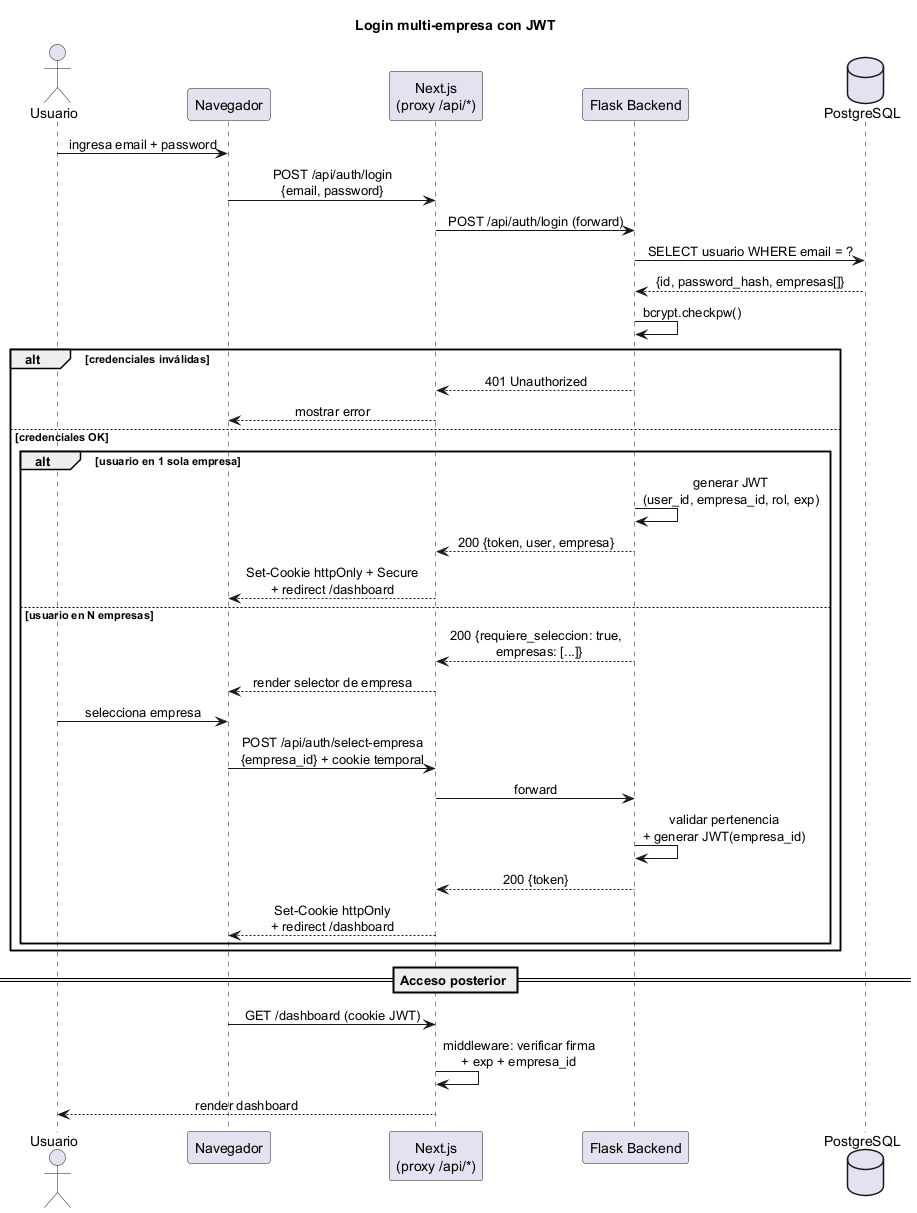
\includegraphics[width=0.95\linewidth]{diagrams/flujo_login_jwt.png}
  \caption{Diagrama de secuencia del login multi-empresa con JWT.}
  \label{fig:flujo_login_jwt}
\end{figure}

\paragraph{Flujo de enrolamiento de dispositivos}

\begin{enumerate}
    \item Un administrador o empleador accede a POST /api/dispositivos/generar-pin desde el panel web, especificando un nombre para el dispositivo. El backend genera un PIN alfanumérico de 8 caracteres (ej. A3B9XK2M) usando secrets.choice() y lo inserta en la tabla dispositivos con enrolado = FALSE.
    \item El administrador ingresa el PIN en la interfaz web del ESP32-CAM (/wifi-setup).
    \item Al guardar la configuración, el ESP32-CAM envía POST /api/dispositivos/enrolar con el PIN, su MAC address y su IP local.
    \item El backend valida el PIN, asocia la MAC y la IP al dispositivo, marca enrolado = TRUE y limpia el PIN para que no pueda ser reutilizado.
    \item A partir de este momento, el ESP32-CAM envía heartbeats periódicos y el backend lo reconoce como dispositivo autorizado de la empresa.
\end{enumerate}

\paragraph{Heartbeat y Last Will Testament (LWT)}

El ESP32-CAM publica periódicamente (cada 30 segundos) un mensaje JSON en el tópico esp32/heartbeat/<MAC> con su MAC, timestamp e IP. El backend actualiza el campo ultimo\_heartbeat y marca el estado como activo. Al conectarse al broker MQTT, el ESP32-CAM configura un mensaje LWT en el tópico esp32/lwt/<MAC> con \{"estado": "inactivo"\}. Si el dispositivo se desconecta abruptamente, el broker publica automáticamente el LWT, y el backend marca el dispositivo como inactivo.

Además del LWT y el watchdog pasivo, se implementó un ping activo como tercera capa de detección: un hilo device\_pinger() publica periódicamente (cada 30 segundos) un mensaje en el tópico esp32/ping/<MAC>. El ESP32-CAM, al recibirlo, responde inmediatamente publicando un heartbeat con el campo "pong": true. Si el backend no recibe respuesta dentro de 60 segundos, marca el dispositivo como inactivo. Este mecanismo permite detectar desconexiones incluso cuando el mensaje LWT no llega al broker (por ejemplo, por pérdida abrupta de conectividad de red). Adicionalmente, un hilo device\_watchdog ejecutado cada 60 segundos verifica qué dispositivos no han enviado heartbeat en más de 90 segundos y los marca como inactivos, constituyendo una capa de respaldo adicional.

\subsubsection{Implementación}

\paragraph{Módulo de autenticación}

El módulo routes/auth.py implementa:

\begin{itemize}
    \item login(): Valida credenciales con bcrypt, determina la empresa (con selección múltiple si aplica), vincula al trabajador con su persona\_id si el rol es trabajador, y genera el token JWT.
    \item register(): Permite a administradores y empleadores crear nuevos usuarios, asignándoles rol y empresa. Si el email ya existe, se agrega la nueva asociación usuario\_empresa en lugar de duplicar el usuario.
    \item me(): Retorna los datos del usuario autenticado, incluyendo sus empresas y rol actual.
    \item cambiar\_password(): Permite al usuario cambiar su contraseña validando la actual.
    \item generar\_pin\_enrolamiento(): Crea un PIN para enrolar un nuevo dispositivo.
    \item enrolar\_dispositivo(): Valida el PIN y completa el enrolamiento del ESP32-CAM.
    \item listar\_usuarios(), eliminar\_usuario(), listar\_empresas(), crear\_empresa(): Operaciones administrativas con control de roles.
    \item register\_company(): Endpoint público POST /api/auth/register-company que permite el auto-registro de una nueva empresa. Recibe los datos de la organización (nombre, RUT, email, teléfono, dirección) y del usuario administrador (nombre, email, contraseña). En una única transacción atómica crea la empresa, el usuario con hash bcrypt, y la asociación usuario\_empresa con rol admin. Retorna un token JWT para autenticar inmediatamente al nuevo administrador.
\end{itemize}

Los decoradores @token\_required, @token\_opcional y @requiere\_rol se definen en el mismo módulo. El decorador @token\_opcional incluye lógica para inferir la empresa a partir del header X-Device-MAC cuando no hay token JWT presente, buscando la MAC en la tabla de dispositivos. Si la MAC no existe, automáticamente crea un nuevo registro en dispositivos con estado pendiente, lo que permite que los ESP32-CAM comiencen a enviar datos incluso antes de ser formalmente enrolados.

\paragraph{Gestión de dispositivos}

El módulo routes/dispositivos.py implementa:

\begin{itemize}
    \item GET /api/dispositivos: Lista los dispositivos con su estado, MAC, IP y empresa.
    \item PUT /api/dispositivos/<id>: Actualiza el nombre del dispositivo.
    \item DELETE /api/dispositivos/<id>: Elimina un dispositivo (admin) o lo desvincula de la empresa (empleador).
    \item POST /api/dispositivos/verificar: Prueba conectividad con un dispositivo dada su IP, consultando el endpoint /estado del ESP32-CAM.
\end{itemize}

\paragraph{Monitorización vía MQTT}

En el módulo mqtt\_handler.py, la función on\_message maneja los tópicos de heartbeat y LWT:

\begin{itemize}
    \item esp32/heartbeat/<MAC>: Actualiza ultimo\_heartbeat, estado = 'activo' y opcionalmente ip\_local del dispositivo.
    \item esp32/lwt/<MAC>: Marca estado = 'inactivo' en la base de datos.
\end{itemize}

El watchdog (device\_watchdog) ejecuta un barrido inicial al arrancar (todos los dispositivos se marcan inactivos hasta que envíen su primer heartbeat) y luego verifica cada 60 segundos los heartbeats vencidos.

\subsubsection{Pruebas}

Se diseñaron las siguientes pruebas para validar la autenticación, el multi-tenant y el enrolamiento:

\begin{itemize}
    \item \textbf{Prueba de login exitoso}: Enviar credenciales válidas del administrador por defecto (admin@empresa.cl / admin123). Verificar que se reciba un token JWT, los datos del usuario y su empresa. Decodificar el token y verificar que contenga user\_id, empresa\_id y rol = admin.

    \item \textbf{Prueba de login con múltiples empresas}: Crear una segunda empresa y asignar el mismo usuario a ella con rol empleador. Iniciar sesión sin especificar empresa. Verificar que el backend retorne la lista de empresas disponibles. Luego, iniciar sesión especificando una empresa y verificar que el token refleje esa selección.

    \item \textbf{Prueba de rechazo de credenciales inválidas}: Intentar login con contraseña incorrecta. Verificar HTTP 401 y mensaje ``Credenciales inválidas''.

    \item \textbf{Prueba de acceso sin token}: Intentar acceder a GET /api/personas sin enviar header Authorization, desde un cliente sin X-Device-MAC. Verificar que el endpoint responda correctamente (acceso público o con datos limitados según el decorador).

    \item \textbf{Prueba de acceso con rol insuficiente}: Autenticarse como trabajador e intentar crear un turno (POST /api/turnos). Verificar HTTP 403 y mensaje ``Permisos insuficientes''.

    \item \textbf{Prueba de aislamiento multi-tenant}: Crear dos empresas (A y B), registrar una persona en cada una. Autenticarse como empleador de la empresa A y solicitar GET /api/personas. Verificar que solo se retornen las personas de la empresa A.

    \item \textbf{Prueba de generación de PIN}: Autenticarse como empleador y solicitar POST /api/dispositivos/generar-pin. Verificar que se reciba un PIN de 8 caracteres alfanuméricos y que en la base de datos exista un dispositivo con enrolado = FALSE.

    \item \textbf{Prueba de enrolamiento exitoso}: Con un PIN generado, enviar POST /api/dispositivos/enrolar con el PIN, una MAC y una IP. Verificar que el backend marque el dispositivo como enrolado, asocie la MAC y limpie el PIN. Verificar que el mismo PIN no pueda usarse una segunda vez (HTTP 409).

    \item \textbf{Prueba de heartbeat y estado}: Simular heartbeats desde un dispositivo enrolado. Verificar que el estado en la base de datos sea activo. Detener los heartbeats por más de 90 segundos y verificar que el watchdog marque el dispositivo como inactivo.

    \item \textbf{Prueba de LWT}: Conectar el ESP32-CAM al broker MQTT, verificar que el backend reciba el heartbeat y lo marque activo. Desconectar el dispositivo abruptamente (corte de energía). Verificar que el broker publique el LWT y el backend actualice el estado a inactivo en menos de 10 segundos.

    \item \textbf{Prueba de auto-registro de empresa}: Enviar una solicitud a POST /api/auth/register-company con los datos de una nueva empresa y su administrador. Verificar que se cree la empresa en la base de datos, que el usuario administrador se cree con contraseña encriptada (bcrypt), que exista la asociación usuario\_empresa con rol admin, y que el backend retorne un token JWT válido que permita acceder a endpoints protegidos. Verificar que un segundo intento con el mismo email de administrador retorne HTTP 409 (Conflicto).
\end{itemize}

\subsubsection{Refinamientos posteriores}

\begin{itemize}
    \item "\textbf{token\_opcional}": el decorador token\_opcional, que permite que un mismo endpoint acepte tanto usuarios web autenticados por JWT como dispositivos ESP32 identificados por el header X-Device-MAC, inicialmente creaba un registro nuevo en dispositivos si la MAC no existía en la base de datos. Este comportamiento se eliminó: ahora el decorador únicamente busca y vincula dispositivos ya existentes, dejando la creación exclusivamente al flujo explícito de enrolamiento con PIN. El cambio cierra una vía por la que un dispositivo no autorizado podía aparecer en el sistema sin pasar por el control del administrador o empleador.

    \item \textbf{PIN de enrolamiento por empresa}: la generación de PIN (POST /api/auth/dispositivos/generar-pin) quedó condicionada al rol de quien la solicita: un administrador puede generar el PIN para cualquier empresa indicada en la petición, mientras que un empleador solo puede generarlo para la empresa a la que pertenece (request.empresa\_id). El dispositivo creado queda asociado a esa empresa desde el momento de la generación del PIN, reforzando el aislamiento multi-tenant también a nivel de hardware enrolado.
\end{itemize}


%% ============================================================
%% ITERACIÓN 6: Módulo antifraude y validación previa a la captura
%% ============================================================

\subsection{Iteración 6: Módulo antifraude y validación previa a la captura}

Esta iteración implementa la prevención de suplantación de identidad en el ESP32-CAM mediante detección física de presencia, control de iluminación y procesamiento biométrico. Si bien el plan original contemplaba un sensor infrarrojo (IR) dedicado para detectar intentos de suplantación con fotografías, el enfoque implementado evolucionó hacia una solución de múltiples capas que resultó más robusta y prescindió del sensor IR adicional.

\subsubsection{Análisis}

El análisis de escenarios de suplantación identificó los siguientes vectores de ataque potenciales contra el sistema de reconocimiento facial del ESP32-CAM:

\begin{itemize}
    \item \textbf{Fotografía impresa}: Un atacante presenta una foto del rostro de un trabajador legítimo frente a la cámara.
    \item \textbf{Pantalla de dispositivo}: Un atacante muestra un video o imagen del trabajador en la pantalla de un teléfono o tablet.
    \item \textbf{Ausencia de presencia real}: La cámara captura sin que haya una persona físicamente frente al dispositivo (falsos positivos del sensor de movimiento).
\end{itemize}

Inicialmente se planificó el uso de un sensor IR dedicado que permitiera detectar la presencia de un rostro real mediante la emisión y recepción de luz infrarroja, cuya reflectancia difiere entre piel humana y superficies planas como papel o pantallas. Sin embargo, durante el desarrollo se identificaron dos factores que motivaron el cambio de estrategia:

\begin{enumerate}
    \item \textbf{Disponibilidad de GPIO}: El ESP32-CAM tiene una cantidad muy limitada de pines GPIO disponibles tras la asignación del bus paralelo de la cámara. Destinar un pin adicional al sensor IR hubiera requerido sacrificar otra funcionalidad (como el sensor PIR de presencia o el control PWM del flash).

    \item \textbf{Madurez del anti-spoofing por software}: DeepFace, la librería seleccionada para el reconocimiento facial, incorpora un detector de suplantación (\textbf{anti-spoofing}) basado en redes neuronales convolucionales que analiza micro-texturas, reflectancia de la piel y profundidad en la imagen capturada. Este detector es capaz de distinguir entre un rostro real tridimensional y una superficie plana (foto, pantalla) con una precisión comparable o superior a la de sensores IR de bajo costo como los inicialmente considerados.
\end{enumerate}

En consecuencia, se adoptó un enfoque de múltiples capas que combina:

\begin{enumerate}
    \item \textbf{Detección física de presencia (PIR)}: Un sensor infrarrojo pasivo (PIR) que detecta el calor corporal, activando el sistema de captura solo cuando hay una persona real frente al dispositivo. Esto elimina falsos positivos del software y reduce el consumo energético del sensor de huella y la cámara.
    \item \textbf{Iluminación controlada (flash PWM)}: Un destello breve y de intensidad moderada (50\% de duty cycle a 5 kHz) que ilumina el rostro durante la captura sin enceguecer a la persona. La respuesta del rostro real a esta fuente de luz puntual difiere de la de una superficie plana, aportando una capa adicional de discriminación.
    \item \textbf{Anti-spoofing por software (DeepFace)}: La capa más potente, que analiza la imagen capturada con un modelo entrenado para detectar intentos de suplantación. Las imágenes que no superan esta validación son rechazadas con una excepción ValueError que el backend traduce en un mensaje de error al ESP32-CAM.
\end{enumerate}

\subsubsection{Diseño}

\paragraph{Sensor PIR como portero del reconocimiento facial}

El lector de huellas se revisa de forma continua, sin depender del PIR: cada 500 milisegundos el sistema consulta al AS608 por si hay un dedo apoyado, de modo que una marcación por huella responda de inmediato sin esperar a que algo más la habilite. El PIR conectado al GPIO12 cumple un rol distinto, acotado al reconocimiento facial: mientras no detecta movimiento, la cámara no se usa para buscar un rostro. Al detectar movimiento (un cambio en la radiación infrarroja del entorno), el sistema enciende el flash a baja intensidad, marca que hay alguien frente al dispositivo y, si en ese momento había un bloqueo temporal del menú activo, lo anula, dando prioridad a la persona que se presentó físicamente. Tras una breve pausa de 800 milisegundos para que la lectura del sensor se estabilice, el sistema queda intentando identificar el rostro cada 6 segundos mientras dure la presencia, siempre que haya conectividad con el backend y hayan pasado al menos 8 segundos desde la última marcación. Si el PIR no vuelve a detectar movimiento durante 15 segundos, se asume que fue una falsa alarma o que la persona se retiró: se apaga el flash y el sistema vuelve a esperar sin haber intentado nada por cámara.

Esta separación evita que el reconocimiento facial, más costoso en procesamiento que la lectura de huella, se ejecute todo el tiempo sin necesidad: solo se activa cuando el PIR confirma que probablemente hay alguien frente al dispositivo.

\paragraph{Control de acceso con cooldown y bloqueo}

Para evitar marcaciones múltiples accidentales y garantizar que cada interacción sea deliberada, se implementan tres mecanismos de control:

\begin{enumerate}
    \item \textbf{Cooldown entre marcaciones} (COOLDOWN\_TIEMPO = 8000 ms): Tras una marcación exitosa, el sistema ignora nuevos intentos durante 8 segundos.
    \item \textbf{Debounce de huella} (FINGER\_DEBOUNCE = 4000 ms): Una misma huella no puede gatillar dos marcaciones en un intervalo menor a 4 segundos, evitando lecturas múltiples del mismo dedo.
    \item \textbf{Bloqueo por menú} (BLOQUEO\_MENU\_MS = 30000 ms): Cuando se utiliza la interfaz web para operaciones administrativas (registro, edición, configuración), se activa un bloqueo de 30 segundos que impide la marcación automática, evitando que la persona que está operando el menú sea registrada inadvertidamente.
\end{enumerate}

\paragraph{Firma de movimiento}

Para detectar si la escena frente a la cámara cambió entre dos capturas consecutivas (lo que indicaría una persona real moviéndose versus una foto estática), se implementa una firma de movimiento que calcula un hash reducido del buffer JPEG:

\begin{itemize}
    \item Se muestrean 128 bytes del frame capturado, distribuidos uniformemente a lo largo del buffer.
    \item Se calcula la suma acumulada de esos bytes, produciendo una firma de 32 bits.
    \item Si la diferencia entre la firma actual y la anterior supera un umbral (UMBRAL\_MOVIMIENTO = 1800), se considera que hubo movimiento real en la escena.
\end{itemize}

\subsubsection{Implementación}

\paragraph{Integración del PIR}

El sensor PIR se conecta al GPIO12 del ESP32-CAM, configurado con resistencia de pull-down interna para evitar lecturas flotantes. En el setup() se incluye una fase de calibración de 3 segundos (delay(3000)) para estabilizar el sensor antes de comenzar el bucle principal.

En el loop(), la lógica de detección sigue el siguiente flujo:

\begin{itemize}
    \item Si el PIR detecta HIGH y el flag "hayAlguienFrenteAlSensor" es falso, se activa el modo alerta y se esperan 800 ms para estabilizar la fuente de alimentación (el capacitor de 1000 $\mu$F del ESP32-CAM necesita recuperarse antes de encender la cámara).
    \item Si el PIR detecta HIGH estando ya en modo alerta, se renueva el timer de actividad.
    \item Si pasan más de 15 segundos sin detección, se desactiva el modo alerta y se retorna a reposo.
\end{itemize}

\paragraph{Flash PWM para iluminación facial}

El flash LED integrado del ESP32-CAM se controla mediante PWM en el GPIO4, configurado como salida LED PWM con frecuencia de 5 kHz y resolución de 8 bits. Durante la captura de una imagen (tanto para registro como para identificación), el flash se activa con un duty cycle del 50\% (FLASH\_PWM\_DUTY\_50 = 128) durante 150-200 milisegundos, tiempo suficiente para que el sensor OV2640 ajuste su exposición.

La secuencia de captura es la siguiente:
\begin{enumerate}
    \item Encender flash al 50\% (ledcWrite(FLASH\_PIN, 128)).
    \item Esperar 150 ms para estabilización del sensor.
    \item Capturar el frame (esp\_camera\_fb\_get()).
    \item Apagar el flash inmediatamente (ledcWrite(FLASH\_PIN, 0)).
    \item Procesar o transmitir el frame.
\end{enumerate}

Este enfoque minimiza el tiempo total de encendido del flash y, por tanto, el consumo eléctrico y la molestia para el usuario.

\paragraph{Señalización mediante el LED verde}

Además de la iluminación para captura, que usa el flash, el resultado de una operación se señaliza con el LED verde integrado en el dispositivo:

\begin{itemize}
    \item \textbf{Éxito} (flashExito()): el LED parpadea dos veces (150 ms encendido, 150 ms apagado en cada destello).
    \item \textbf{Error} (flashError()): no hay señal luminosa propia; la función queda como punto de extensión reservado en el firmware para una señal de error dedicada (por ejemplo, un patrón distinto de parpadeo o un LED rojo adicional).
\end{itemize}

El parpadeo del LED verde permite al usuario confirmar de un vistazo que su marcación se registró, sin necesidad de mirar una pantalla. La ausencia de una señal equivalente para el caso de error es una limitación reconocida del prototipo (Sección~\ref{sec:limitaciones}), ya que actualmente un error solo es visible al consultar la vista web del dispositivo.

\paragraph{Validación anti-spoofing en el backend}

La validación anti-spoofing se ejecuta en el backend, no en el ESP32-CAM, debido a las limitaciones de procesamiento del microcontrolador. La función extraer\_embedding() en routes/facial.py recibe el parámetro anti\_spoofing=True para los endpoints de identificación y verificación, lo que activa el detector de suplantación de DeepFace. Si la imagen no supera la validación (por ser una foto, pantalla o carecer de características faciales reales), DeepFace lanza una excepción ValueError que el backend captura y traduce en una respuesta HTTP 400 con el mensaje ``Spoof detected''.

\subsubsection{Pruebas}

Se diseñaron las siguientes pruebas para validar el módulo antifraude:

\begin{itemize}
    \item \textbf{Prueba de detección PIR}: Situar a una persona a 50 cm del dispositivo. Verificar que el PIR detecte el movimiento en menos de 1 segundo y que el sistema transicione a modo activo. Retirar a la persona y verificar que tras 15 segundos sin detección, el sistema retorne a reposo.

    \item \textbf{Prueba de falsos positivos del PIR}: Dejar el dispositivo en una habitación vacía durante 10 minutos y monitorear los logs. Verificar que no se active el modo de captura sin presencia humana real (tolerancia máxima: 1 falso positivo por hora).

    \item \textbf{Prueba de cooldown}: Realizar una marcación exitosa por huella. Intentar inmediatamente una segunda marcación. Verificar que el sistema rechace el intento por estar en período de cooldown (8 segundos).

    \item \textbf{Prueba de debounce de huella}: Mantener el dedo presionado sobre el sensor AS608 durante 5 segundos. Verificar que solo se registre una marcación, no múltiples.

    \item \textbf{Prueba de bloqueo por menú}: Acceder a la vista /register desde el navegador. Mientras la página está abierta, intentar provocar una marcación automática con huella. Verificar que el sistema esté bloqueado durante 30 segundos.

    \item \textbf{Prueba de anti-spoofing con fotografía}: Imprimir una foto de un rostro registrado y presentarla frente al ESP32-CAM con el PIR activado (para ello, mover la foto simulando una persona). Verificar que DeepFace rechace la imagen con anti\_spoofing=True y que el backend retorne HTTP 400.

    \item \textbf{Prueba de anti-spoofing con pantalla}: Reproducir un video del rostro de una persona registrada en un teléfono móvil y presentarlo frente al ESP32-CAM. Verificar que el sistema rechace la identificación.

    \item \textbf{Prueba de flash PWM}: Durante una captura, medir con un osciloscopio o cámara de alta velocidad que el flash se encienda al 50\% de duty cycle durante no más de 200 ms. Verificar que la iluminación sea suficiente para obtener una imagen nítida del rostro.

    \item \textbf{Prueba de señalización}: Provocar una marcación exitosa y verificar que el LED verde parpadee dos veces. Provocar un error (huella no reconocida) y verificar que no se emita ninguna señal luminosa.
\end{itemize}


%% ============================================================
%% ITERACIÓN 7: Panel web backend e integración con ERP
%% ============================================================

\subsection{Iteración 7: Panel web backend e integración con ERP}

La séptima iteración incorpora el panel de administración web del backend y el módulo de integración con sistemas ERP externos, permitiendo que los datos de asistencia capturados por el dispositivo IoT sean automáticamente transmitidos a plataformas empresariales de recursos humanos o nómina.

\subsubsection{Análisis}

El sistema, hasta esta iteración, permite registrar asistencias y almacenarlas en la base de datos, pero carece de una interfaz administrativa centralizada y de un mecanismo para integrar los datos con sistemas ERP existentes. Se identificaron los siguientes requisitos:

\begin{itemize}
    \item \textbf{Panel web administrativo}: Una interfaz web que permita a administradores y empleadores gestionar personas, turnos, asignaciones, visualizar asistencias, administrar dispositivos enrolados y configurar integraciones ERP. Debe ser accesible vía navegador sin dependencia del ESP32-CAM.
    \item \textbf{API REST completa y documentada}: Todos los blueprints implementados en iteraciones anteriores deben consolidarse como una API REST coherente, con métodos HTTP estándar, respuestas JSON estructuradas y manejo de autenticación por JWT.
    \item \textbf{Integración con ERP vía webhooks}: Permitir configurar múltiples destinos ERP, cada uno con su propia URL de webhook, headers personalizados (ej. tokens de autenticación) y mapeo de campos (field mapping) para adaptar el formato de los datos de asistencia al esquema esperado por cada ERP.
    \item \textbf{Envío automático}: Las asistencias registradas deben enviarse automáticamente a los ERP configurados, en un hilo separado para no bloquear la respuesta HTTP al dispositivo.
    \item \textbf{Test de conectividad}: Cada integración ERP debe poder probarse manualmente desde el panel web antes de activar el envío automático.
\end{itemize}

\subsubsection{Diseño}

\paragraph{Arquitectura del backend}

El backend se organiza en 9 blueprints de Flask, cada uno con responsabilidades bien definidas:

\begin{enumerate}
    \item auth\_bp: Autenticación JWT, registro de usuarios, gestión de empresas, enrolamiento de dispositivos.
    \item personas\_bp: CRUD de personas con consentimiento biométrico y eliminación de datos sensibles.
    \item turnos\_bp: CRUD de turnos con filtro por empresa.
    \item asignaciones\_bp: CRUD de asignaciones persona-turno.
    \item asistencias\_bp: Registro de asistencias individuales y sincronización por lotes.
    \item facial\_bp: Registro, verificación e identificación facial con anti-spoofing y cifrado.
    \item dispositivos\_bp: Gestión de dispositivos enrolados y verificación de conectividad.
    \item logs\_bp: Consulta de logs de sincronización y logs biométricos.
    \item erp\_bp: CRUD de integraciones ERP, envío de datos y test de conectividad.
\end{enumerate}

\paragraph{Diseño del módulo ERP}

La integración con ERP se basa en el patrón webhook saliente: cuando se registra una asistencia, el backend notifica a cada ERP configurado mediante una solicitud HTTP POST al webhook correspondiente, con los datos de la marcación en el cuerpo JSON.

Cada integración ERP se configura con los siguientes parámetros:

\begin{itemize}
    \item nombre: Identificador descriptivo (ej. ``Softland RRHH'').
    \item tipo: Clasificación del ERP (generic, softland, defontana, sap).
    \item webhook\_url: Endpoint HTTP donde el ERP espera recibir los datos.
    \item headers: Objeto JSON con headers HTTP personalizados (ej. \{"Authorization": "Bearer <token>"\}).
    \item field\_map: Objeto JSON que mapea los campos estándar del sistema (rut, nombre, tipo, metodo, fecha\_hora) a los nombres de campo esperados por el ERP.
    \item envio\_auto: Booleano que indica si el envío se realiza automáticamente al registrar cada asistencia, o solo manualmente.
    \item activo: Booleano para habilitar o deshabilitar temporalmente la integración sin eliminarla.
\end{itemize}

El field mapping permite adaptar el formato de salida sin modificar el código del backend. Por ejemplo, un ERP que espera los campos employee\_id, timestamp y event\_type puede configurarse con:
\begin{verbatim}
{"rut": "employee_id", "fecha_hora": "timestamp", "tipo": "event_type"}
\end{verbatim}

\begin{figure}[H]
  \centering
  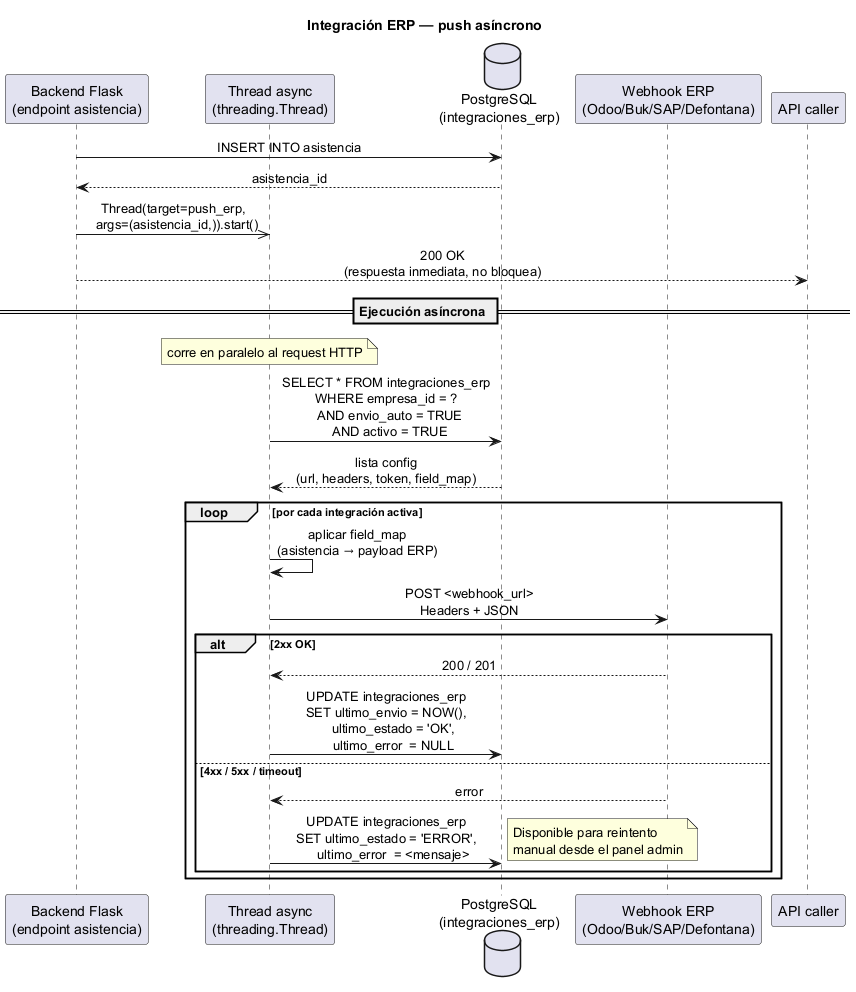
\includegraphics[width=0.95\linewidth]{diagrams/flujo_integracion_erp.png}
  \caption{Diagrama de secuencia de la integración ERP: push asíncrono con field mapping.}
  \label{fig:flujo_erp}
\end{figure}

\subsubsection{Implementación}

\paragraph{Panel web del backend}

Para complementar el backend, se desarrolló un panel web independiente (Next.js 16 \cite{nextjs_docs} con React 19 y TypeScript) cuyo módulo principal es la gestión del dispositivo IoT. Este panel, accesible desde cualquier navegador moderno, permite al administrador:

\begin{itemize}
    \item Visualizar el estado online/offline de cada dispositivo enrolado en tiempo real mediante tarjetas con código de colores, indicador animado (live-dot) y la IP como enlace clickable con la leyenda ``Misma red requerida''.
    \item Generar el PIN de 8 caracteres necesario para enrolar un nuevo ESP32-CAM.
    \item Probar la conectividad activa con un dispositivo específico consultando su endpoint /estado (variable NEXT\_PUBLIC\_DEVICE\_BASE\_URL, por defecto http://192.168.4.1).
    \item Renombrar y eliminar dispositivos registrados.
    \item Acceder a los logs de sincronización generados por el dispositivo.
    \item Acceder a las funcionalidades complementarias de gestión: personas, turnos, asignaciones, asistencias, integración ERP, usuarios y empresas.
\end{itemize}

El estado en tiempo real se obtiene mediante dos mecanismos complementarios. El principal es un hook useDeviceWebSocket que utiliza EventSource para conectarse directamente al endpoint SSE del backend (http://localhost:5000/sse/devices), recibiendo eventos con el id, nombre, IP, estado y timestamp del último heartbeat de cada dispositivo. Como respaldo, un temporizador ejecuta una consulta REST cada 15 segundos (GET /api/dispositivos) para actualizar el estado si la conexión SSE se interrumpe. El estado online se calcula verificando que el campo estado sea 'activo' y que el ultimo\_heartbeat esté dentro de los últimos 5 minutos; si alguna condición falla, el dispositivo se considera offline.

El panel web se comunica con el backend Flask mediante un proxy interno (app/api/\_proxy.ts) que reenvía las peticiones REST a la API, evitando problemas de CORS. La conexión SSE, por su parte, se realiza directamente al backend en el puerto 5000 sin pasar por el proxy, ya que requiere una conexión persistente text/event-stream. La aplicación está protegida por un middleware de autenticación que valida el token JWT y restringe el acceso según el rol del usuario (admin, empleador, trabajador). El frontend se compila con Docker en un build multi-etapa usando output: 'standalone' para producir una imagen optimizada lista para producción.

Para mantener la consistencia visual entre el panel web y la interfaz embebida del ESP32-CAM, las 9 vistas HTML del dispositivo (index.html, register.html, gestion.html, personas.html, turnos.html, asignaciones.html, asistencias.html, logs.html y wifi-setup.html) fueron actualizadas para adoptar la misma paleta oscura, tipografía y sistema de componentes del panel SAS. Se utilizaron variables CSS para la paleta cromática, diseño basado en tarjetas (cards) para la disposición del contenido, y componentes reutilizables para botones, tablas y formularios, logrando que ambas interfaces presenten una experiencia de usuario unificada.

Adicionalmente, el panel web incorpora las siguientes funcionalidades complementarias:

\begin{itemize}
    \item \textbf{Auto-registro de empresas}: La pantalla de inicio de sesión incluye un modo de registro que permite a nuevas empresas crear su cuenta directamente, invocando al endpoint público POST /api/auth/register-company. El formulario solicita nombre de la empresa y datos del administrador de la empresa (nombre, email, contraseña), y al enviarlo crea la organización, el usuario administrador y retorna un token JWT para acceso inmediato.
    \item \textbf{Captura facial por webcam}: El formulario de registro facial en el panel web utiliza la API navigator.mediaDevices.getUserMedia() para capturar fotografías directamente desde la cámara del navegador, eliminando la necesidad de subir archivos desde el sistema de archivos local. La interfaz permite visualizar la vista previa en vivo, capturar, previsualizar y confirmar o repetir la toma, con liberación adecuada del stream al cancelar.
    \item \textbf{Edición de usuarios del sistema}: Los administradores y empleadores pueden editar los datos de los usuarios del sistema (nombre, email, rol, contraseña, estado activo/inactivo) mediante un formulario modal que reutiliza la interfaz de registro en modo edición. Las actualizaciones son parciales: solo se envían los campos modificados.
\end{itemize}

\paragraph{Endpoint de configuración ERP para el ESP32-CAM}

Para que el ESP32-CAM pueda notificar asistencias directamente a los ERP configurados (incluso si el backend central no está disponible), se implementó el endpoint GET /api/dispositivos/erp-config, que retorna la lista de integraciones ERP activas con envío automático habilitado. El ESP32-CAM consulta este endpoint cada hora y almacena la configuración en /erp-config.json, permitiéndole enviar marcaciones a los ERP incluso durante desconexiones parciales.

\paragraph{Contraseñas para autenticación de dispositivos}

Para reforzar la seguridad en la comunicación entre el backend y los ESP32-CAM enrolados, se implementó un sistema de contraseñas de dispositivo que permite al administrador generar, gestionar y verificar credenciales específicas para cada terminal IoT. El flujo contempla cuatro operaciones:

\begin{itemize}
    \item \textbf{Generar contraseña} (POST /api/dispositivos/<id>/generar-password): El administrador solicita una nueva contraseña de 12 caracteres alfanuméricos, generada mediante secrets.choice(). El backend almacena el hash SHA256 de la contraseña, la versión en texto plano (temporal) y marca la contraseña como pendiente (password\_pendiente = TRUE). La respuesta incluye la contraseña en texto plano para que el administrador la proporcione al dispositivo.
    \item \textbf{Verificar contraseña pendiente} (GET /api/dispositivos/check-password): El ESP32-CAM, al iniciar, consulta este endpoint enviando su MAC address como header X-Device-MAC. Si hay una contraseña pendiente, el backend la retorna en texto plano para que el dispositivo la aplique localmente.
    \item \textbf{Confirmar contraseña} (POST /api/dispositivos/confirmar-password): Una vez que el dispositivo ha aplicado la contraseña localmente, confirma al backend, que limpia el texto plano (password\_plain = NULL) y desmarca el estado pendiente. A partir de este momento, solo el hash SHA256 permanece almacenado.
    \item \textbf{Eliminar contraseña} (DELETE /api/dispositivos/<id>/password): El administrador puede eliminar la contraseña de un dispositivo, limpiando el hash y el texto plano.
\end{itemize}

En el panel web, la sección de gestión de dispositivos incorpora botones para generar, regenerar y eliminar contraseñas, así como indicadores visuales del estado de la contraseña (tiene o no tiene, pendiente o confirmada).

\paragraph{Módulo de integración ERP}

El módulo routes/erp.py implementa:

\begin{itemize}
    \item \textbf{enviar\_asistencia\_a\_erps()}: Función central que itera sobre las integraciones ERP activas de una empresa, transforma los datos de la asistencia según el field mapping configurado, y envía una solicitud POST al webhook con los headers personalizados. Registra el resultado (ok o error) en la tabla integraciones\_erp (columnas ultimo\_envio y ultimo\_estado).

    \item \textbf{\_disparar\_erp\_push()}: Wrapper que ejecuta enviar\_asistencia\_a\_erps() en un hilo daemon separado, evitando que la latencia de los ERP externos afecte el tiempo de respuesta al ESP32-CAM. Esta función se invoca automáticamente desde create\_asistencia() y sync\_asistencias() cada vez que se registra una asistencia.

    \item \textbf{CRUD de integraciones}: Endpoints REST para crear, listar y eliminar configuraciones ERP.

    \item \textbf{Test de conectividad} (POST /api/erp/<id>/test): Envía un payload de prueba con datos ficticios al webhook configurado y retorna el código de respuesta y el cuerpo recibido.

    \item \textbf{Envío manual} (POST /api/erp/<id>/enviar): Envía las últimas 200 asistencias de la empresa al ERP seleccionado, útil para cargas históricas o reprocesamiento.

    \item \textbf{Estado de integración} (GET /api/erp/<id>/estado): Retorna el último envío y su estado.
\end{itemize}

\paragraph{Control remoto de dispositivos ESP32}

Se implementaron tres endpoints en routes/dispositivos.py que permiten controlar remotamente los ESP32-CAM enrolados mediante comandos MQTT:

\begin{itemize}
    \item \textbf{Registrar huella} (POST /api/dispositivos/<id>/registrar-huella): Recibe un persona\_id y envía al dispositivo el comando para iniciar el enrolamiento de una huella digital. Verifica que el dispositivo exista, que pertenezca a la empresa del usuario autenticado, y que la persona exista en la misma empresa. Utiliza enviar\_comando\_dispositivo(mac, 'registrar\_huella') para publicar el comando en backend/comando/<MAC>/registrar\_huella. El resultado del enrolamiento se recibe luego por el tópico esp32/huella/resultado/\#.

    \item \textbf{Reiniciar dispositivo} (POST /api/dispositivos/<id>/reiniciar): Envía el comando reiniciar al ESP32-CAM, provocando un reinicio remoto del dispositivo. Útil para recuperar un dispositivo que presenta fallos de conectividad o para aplicar cambios de configuración. Si el cliente MQTT no está disponible, retorna HTTP 503.

    \item \textbf{Reconectar Wi-Fi} (POST /api/dispositivos/<id>/wifi-reconnect): Envía el comando wifi-reconnect para que el dispositivo reinicie su conexión Wi-Fi. Permite recuperar un dispositivo que ha perdido la conectividad sin necesidad de intervención física.
\end{itemize}

Los tres endpoints están protegidos con \textbf{"@requiere\_rol('admin', 'empleador')"} y verifican que el dispositivo pertenezca a la empresa del usuario autenticado. Los comandos se publican en el tópico backend/comando/<MAC>/<comando> mediante la función enviar\_comando\_dispositivo() del módulo mqtt\_handler.py.

\subsubsection{Pruebas}

Se diseñaron las siguientes pruebas para validar el panel web para la gestión del dispositivo y la integración ERP:

\begin{itemize}
    \item \textbf{Prueba de streaming SSE}: Conectar el navegador a http://localhost:5000/sse/devices y verificar que se reciban eventos text/event-stream con datos JSON de los dispositivos. Simular un heartbeat desde un ESP32-CAM y verificar que el evento SSE refleje el cambio a estado activo. Desconectar el dispositivo y verificar que el evento SSE refleje el estado inactivo.

    \item \textbf{Prueba de fallback polling}: Interrumpir la conexión SSE (deteniendo el servidor backend momentáneamente). Verificar que el panel web continúe mostrando el estado de los dispositivos mediante las consultas REST periódicas (cada 15 segundos) y que al restaurar la conexión SSE se retome el streaming.

    \item \textbf{Prueba de indicador visual de dispositivo}: Verificar que cada tarjeta de dispositivo en el panel web muestre: la dirección IP como enlace clickable que abre http://<ip>/ en una nueva pestaña, un indicador animado verde/rojo (live-dot) que refleje el estado online/offline, y la leyenda ``Misma red requerida'' como sugerencia contextual.

    \item \textbf{Prueba de navegación en panel web}: Acceder a las rutas principales del backend (/health, /api/personas, /api/asistencias) sin autenticación y verificar que respondan correctamente (HTTP 200 con acceso público o HTTP 401 cuando se requiera token).

    \item \textbf{Prueba de creación de integración ERP}: Autenticarse como empleador y enviar POST /api/erp con nombre, tipo, webhook URL (usando un servidor de prueba como https://webhook.site) y field mapping. Verificar que la integración se cree con activo = TRUE y envio\_auto = TRUE.

    \item \textbf{Prueba de test de webhook}: Ejecutar POST /api/erp/<id>/test para la integración creada. Verificar que el webhook de prueba reciba un payload JSON con datos ficticios (rut = '11.111.111-1', nombre = "Test Usuario", tipo = "entrada"). Verificar que el estado se actualice en la base de datos.

    \item \textbf{Prueba de envío automático}: Registrar una asistencia real (POST a /api/asistencias) para una persona de la empresa configurada. Verificar que el servidor de prueba del webhook reciba automáticamente el payload con los datos de la asistencia.

    \item \textbf{Prueba de field mapping}: Configurar un ERP con field mapping \{"rut": "employee\_id", "tipo": "event"\}. Registrar una asistencia y verificar que el webhook reciba el payload con los campos renombrados (employee\_id en lugar de rut, event en lugar de tipo).

    \item \textbf{Prueba de envío asíncrono}: Medir el tiempo de respuesta del endpoint POST /api/asistencias cuando hay un ERP configurado cuyo webhook tarda 5 segundos en responder. Verificar que la respuesta al cliente sea inmediata (menor a 200 ms) y que el envío al ERP ocurra en segundo plano.

    \item \textbf{Prueba de tolerancia a fallos ERP}: Configurar un webhook que retorne HTTP 500. Registrar una asistencia y verificar que el sistema no falle; el error debe quedar registrado en ultimo\_estado de la integración y la asistencia debe persistirse correctamente en la base de datos.

    \item \textbf{Prueba de sincronización de configuración ERP al ESP32-CAM}: Simular la consulta GET /api/dispositivos/erp-config desde el ESP32-CAM (con header X-Device-MAC). Verificar que retorne solo las integraciones activas con envío automático de la empresa correspondiente.

    \item \textbf{Prueba de envío manual por lote}: Ejecutar POST /api/erp/<id>/enviar y verificar que se envíen correctamente los registros de asistencia recientes al webhook del ERP.
\end{itemize}

\subsubsection{Refinamientos posteriores}

\begin{itemize}
    \item \textbf{Reasignación de dispositivos entre empresas}: se agregó el endpoint PUT /api/dispositivos/<id>/reasignar, restringido al rol admin, que permite mover un dispositivo ya enrolado de una empresa a otra actualizando su columna empresa\_id. Esto resuelve el caso de dispositivos físicos que cambian de destino (por ejemplo, al reasignar hardware entre sucursales o clientes) sin requerir un nuevo proceso de enrolamiento con PIN.

    \item \textbf{Zona horaria de Chile en la integración ERP}: los timestamps enviados a los webhooks ERP se normalizan a America/Santiago mediante el módulo estándar zoneinfo, con conversión explícita antes de formatear cada fecha\_hora y timestamp del payload. Esto evita ambigüedades cuando el servidor del backend opera en UTC y el sistema ERP de destino espera horarios locales.

    \item \textbf{Soporte de múltiples fotos en el panel web}: el panel de administración construido con Next.js incorpora en la vista de cada persona la visualización de las fotos de referencia asociadas a sus distintos encodings\_faciales, reflejando en la interfaz la capacidad de multi-encoding ya descrita en la Sección 2.3.10. Asimismo, en los despliegues multi-empresa la interfaz incorpora una indicación visual de la empresa a la que pertenece cada registro, relevante para el rol admin, que puede ver datos de más de una organización.
\end{itemize}


%% ============================================================
%% ITERACIÓN 8: Sincronización diferida, logs y cierre del proyecto
%% ============================================================

\subsection{Iteración 8: Sincronización diferida, logs y cierre del proyecto}

Esta iteración integra la sincronización diferida entre el ESP32-CAM y el backend, la capa de auditoría y logs del sistema, y las herramientas de diagnóstico.

\subsubsection{Análisis}

Para que el prototipo sea viable en entornos reales, debe garantizar que ningún dato se pierda durante períodos de desconexión y que todas las operaciones críticas queden registradas para auditoría. Los requisitos identificados son:

\begin{itemize}
    \item \textbf{Sincronización diferida de asistencias}: Los registros de asistencia generados offline (marcados con sincronizado = false) deben enviarse automáticamente al backend cuando se restablezca la conectividad. El proceso debe ser idempotente: si un registro ya existe en el backend, no debe duplicarse.
    \item \textbf{Sincronización diferida de entidades}: Las personas, turnos y asignaciones creados localmente durante el modo offline deben sincronizarse con el backend, resolviendo conflictos de identificadores (IDs locales con prefijo local- versus IDs del backend).
    \item \textbf{Sincronización de configuración ERP}: La configuración de integraciones ERP debe poder descargarse desde el backend para que el ESP32-CAM pueda enviar datos de asistencia directamente a los ERP configurados.
    \item \textbf{Logs de sincronización}: Cada operación de sincronización debe registrarse en la base de datos con el conteo de registros enviados y procesados correctamente, permitiendo auditoría posterior.
    \item \textbf{Logs biométricos}: Todas las operaciones de registro, verificación e identificación facial deben quedar registradas con timestamp, resultado e IP de origen, para cumplimiento normativo.
    \item \textbf{Watchdog de dispositivos}: El backend debe monitorear continuamente el estado de los dispositivos enrolados, detectando aquellos que han dejado de comunicarse y marcándolos como inactivos.
    \item \textbf{Herramientas de diagnóstico}: Se requiere un script de prueba que permita simular asistencias faciales usando fotos almacenadas, facilitando las pruebas del sistema sin necesidad del hardware.
\end{itemize}

\subsubsection{Diseño}

\paragraph{Proceso de sincronización diferida}

El ESP32-CAM ejecuta la sincronización en dos momentos:
\begin{enumerate}
    \item \textbf{Al iniciar}: Si hay conectividad, llama a sincronizarPendientes() que ejecuta en secuencia:
    \begin{itemize}
        \item sincronizarTurnosPendientes(): Envía los turnos con sincronizado = false al backend vía POST, y actualiza sus backend\_id.
        \item sincronizarAsignacionesPendientes(): Similar para asignaciones, dependiendo de que los turnos referenciados ya tengan backend\_id.
        \item sincronizarAsistencias(): Envía un lote de asistencias con sincronizado = false vía POST /api/asistencias/sync.
    \end{itemize}
    \item \textbf{Periódicamente}: Cada 5 minutos (300,000 ms), se ejecuta sincronizarPendientes() en el bucle principal.
\end{enumerate}

Además, el ESP32-CAM consulta GET /api/dispositivos/erp-config cada hora (360,000 ms) para mantener actualizada su configuración local de webhooks ERP.

\begin{figure}[H]
  \centering
  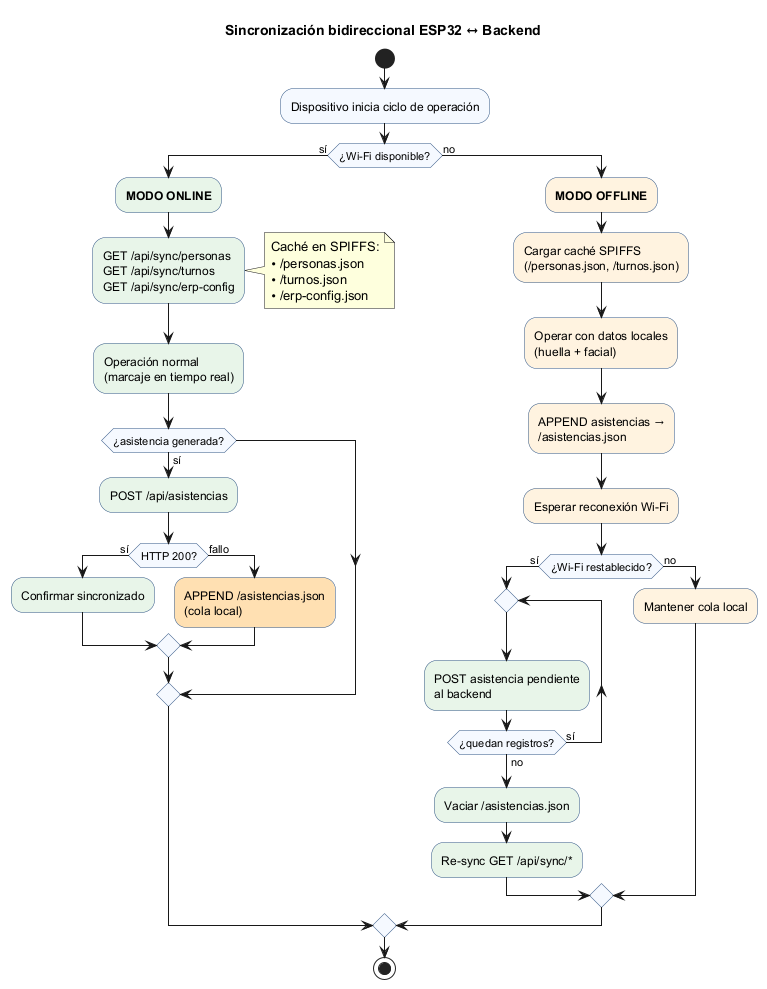
\includegraphics[width=0.95\linewidth]{diagrams/flujo_sincronizacion_bidireccional.png}
  \caption{Diagrama de actividad: sincronización bidireccional entre los modos online y offline del ESP32-CAM.}
  \label{fig:flujo_sync}
\end{figure}

\paragraph{Deduplicación en el backend}

El endpoint POST /api/asistencias/sync implementa una verificación previa a la inserción: para cada registro del lote, consulta si ya existe una asistencia de la misma persona (persona\_id), mismo tipo (entrada/salida), mismo turno\_id y misma fecha (DATE(fecha\_hora) = CURRENT\_DATE). Si existe, omite la inserción. Esta verificación por turno\_id permite que un trabajador registre múltiples asistencias en un mismo día si pertenece a distintos turnos (por ejemplo, jornada diurna y jornada nocturna), sin generar duplicados dentro del mismo turno. Garantiza idempotencia ante reenvíos.

\paragraph{Tablas de auditoría}

\begin{itemize}
    \item sincronizacion\_log: Registra cada operación de sincronización con: dispositivo de origen, cantidad de registros enviados, cantidad procesada correctamente, estado y detalle.
    \item logs\_biometricos: Registra cada operación biométrica con: persona, dispositivo, timestamp, tipo de operación (registro, verificación, identificación), resultado (éxito, fallo, duplicado, no\_encontrado) e IP de origen.
    \item eliminaciones\_biometricas: Registra cada eliminación de datos biométricos con: persona, embedding anterior (cifrado), ruta de la foto eliminada y usuario solicitante.
\end{itemize}

\paragraph{Panel de visualización de logs}

El backend expone dos conjuntos de endpoints para consulta de logs:
\begin{itemize}
    \item GET /api/logs: Lista los registros de sincronización, con filtro por empresa para roles no-admin.
    \item DELETE /api/logs: Permite limpiar los logs (admin limpia todo, empleador limpia los de su empresa).
    \item El ESP32-CAM expone GET /api/logs que retorna el buffer de logs en formato HTML, y /api/logs/clear para limpiarlo.
\end{itemize}

\paragraph{Script de simulación de asistencia facial}

Se desarrolló deteccion.py, un script de línea de comandos que permite probar el flujo de reconocimiento facial sin necesidad del ESP32-CAM. El script escanea las fotos almacenadas localmente para el ambiente de pruebas, presenta un menú interactivo para seleccionar una de ellas, ejecuta el proceso de identificación 1:N contra la base de datos y registra la asistencia correspondiente. Es útil para pruebas de regresión rápida y demostraciones.

\subsubsection{Implementación}

\paragraph{Sincronización en el ESP32-CAM}

Las funciones de sincronización siguen un patrón común:

\begin{enumerate}
    \item Verificar conectividad (isOnline y WiFi.status() == WL\_CONNECTED).
    \item Cargar los datos locales desde LittleFS.
    \item Iterar sobre los registros con sincronizado = false.
    \item Para cada uno, construir el payload JSON y enviarlo al backend vía HTTP POST.
    \item Si el backend responde con éxito (HTTP 200/201), marcar sincronizado = true y actualizar el backend\_id si corresponde.
    \item Persistir los cambios en LittleFS.
\end{enumerate}

Para las personas, además del envío de pendientes, se implementa la descarga completa desde el backend (sincronizarPersonasDesdeBackend()) que sobrescribe el archivo local si no hay registros locales pendientes, manteniendo el ESP32-CAM actualizado con los datos del servidor.

\paragraph{Campo colación en turnos}

Los turnos incorporaron los campos con\_colacion (booleano), colacion\_inicio (TIME) y colacion\_fin (TIME) para modelar el horario de colación de los trabajadores, en cumplimiento del artículo 34 del Código del Trabajo chileno. En la tabla turnos de PostgreSQL se almacenan como TIME (o NULL si con\_colacion = FALSE). Los endpoints CRUD de routes/turnos.py gestionan estos campos: al crear un turno, se envían con\_colacion, colacion\_inicio y colacion\_fin; al actualizar, se usa COALESCE para preservar valores existentes si no se envían. Las consultas GET retornan los horarios como string o null según corresponda. El campo turno\_id se agregó también a la tabla asistencias para asociar cada marcación al turno bajo el cual se registró, permitiendo el cálculo preciso de horas trabajadas descontando la colación.

\paragraph{Sincronización de asistencias por lote}

La función sincronizarAsistencias() en el ESP32-CAM es especialmente relevante porque maneja el caso más frecuente de datos offline: un trabajador marcó entrada y salida durante el día sin conexión. La función:

\begin{enumerate}
    \item Carga asistencias.json y filtra las que tengan sincronizado = false.
    \item Construye un JSON con estructura \{"registros": [...]\}.
    \item Lo envía a POST /api/asistencias/sync.
    \item Si el backend retorna HTTP 200, marca todos los registros enviados como sincronizados.
\end{enumerate}

\paragraph{Sincronización en el backend}

El endpoint POST /api/asistencias/sync en routes/asistencias.py recibe el lote e itera sobre cada registro, aplicando la verificación de duplicados y realizando la inserción. También dispara el envío a ERP para cada asistencia nueva.

\paragraph{Watchdog y ping activo de dispositivos}

La detección de desconexión de dispositivos se implementó con tres capas complementarias:

\begin{enumerate}
    \item \textbf{LWT (instantáneo)}: Al conectarse al broker MQTT, el ESP32-CAM configura un mensaje Last Will en esp32/lwt/<MAC>. Si el dispositivo se desconecta abruptamente, el broker publica automáticamente el LWT y el backend marca el dispositivo como inactivo de inmediato.
    \item \textbf{Ping activo (device\_pinger)}: Un hilo separado publica periódicamente (cada 30 segundos) un mensaje en el tópico esp32/ping/<MAC>. El ESP32-CAM, al recibirlo, responde publicando un heartbeat con el campo "pong": true. Si el backend no recibe respuesta dentro de 60 segundos, marca el dispositivo como inactivo. Este mecanismo funciona incluso si el mensaje LWT no fue entregado.
    \item \textbf{Watchdog pasivo (device\_watchdog)}: Un hilo ejecutado cada 60 segundos realiza un barrido inicial al arrancar el backend (todos los dispositivos se marcan inactivo) y luego verifica periódicamente qué dispositivos no han enviado heartbeat en más de 90 segundos, marcándolos como inactivos.
\end{enumerate}

Esta arquitectura de tres capas asegura que ninguna desconexión pase desapercibida: el LWT atrapa las desconexiones abruptas detectadas por el broker; el ping activo detecta silencios de red donde el LWT no alcanza a publicarse; y el watchdog pasivo actúa como respaldo final para cualquier caso no cubierto por las capas anteriores.

\paragraph{Herramienta de simulación facial}

Como complemento durante el desarrollo se implementó deteccion.py, un script de línea de comandos que permitió probar el flujo de reconocimiento facial sin necesidad del ESP32-CAM. El script se conectaba directamente a PostgreSQL, ejecutaba DeepFace (Facenet + detector configurable + anti-spoofing) sobre imágenes almacenadas localmente para el ambiente de pruebas, y registraba asistencias de prueba en la base de datos. En las etapas finales del proyecto, esta funcionalidad de simulación fue absorbida por la suite de pruebas automatizadas (con mocks de DeepFace, OpenCV y PostgreSQL en Docker), que ofrece mayor repetibilidad y cobertura sin dependencia del sistema de archivos local.

\paragraph{Flujo operacional consolidado}
\label{sec:flujo_operacional_consolidado}

Con todos los componentes del sistema ya construidos (enrolamiento por PIN, reconocimiento biométrico, almacenamiento offline, sincronización diferida e integración ERP), la Fig.~\ref{fig:flujo_operacional} consolida el camino completo que sigue una marcación, cubriendo tanto el caso con conexión a internet como el caso sin ella, tal como quedó implementado al cierre del proyecto.

El flujo comienza cuando el sensor PIR detecta presencia frente al dispositivo y se ejecuta la captura biométrica (huella mediante el AS608 o rostro mediante la cámara OV2640). A partir de ahí, el firmware evalúa isCloudReady(): si el dispositivo está conectado a internet y enrolado, la marcación se envía de inmediato al backend por HTTP (POST /api/facial/identificar para rostro, o POST /api/asistencias para huella). Si cualquiera de esas dos condiciones falla, la marcación se guarda localmente en asistencias.json (LittleFS) con la marca sincronizado=false, se muestra el resultado en el panel embebido sin esperar respuesta del servidor, y el dispositivo queda a la espera de que la conexión se restablezca para ejecutar sincronizarPendientes(), que vacía la cola completa hacia el backend.

Ambos caminos, el envío inmediato y la sincronización diferida, terminan convergiendo en el mismo punto: el backend valida la huella o el rostro contra los registros almacenados (encodings\_faciales o el identificador de huella) y persiste el resultado en la tabla asistencias de PostgreSQL. Si la identificación es exitosa, el backend responde 200 OK, dispara en un hilo aparte el envío hacia los sistemas ERP configurados, y el firmware ejecuta flashExito(), que hace parpadear el LED verde del dispositivo dos veces. Si no hay coincidencia o la imagen no cumple el filtro de calidad, el backend responde con un código de error (404 o 400) y la operación queda registrada en logs\_biometricos para su auditoría posterior; en este caso el firmware invoca flashError(), una función que existe en el código como punto de extensión para una señal de error distinta, pero que actualmente no tiene ninguna acción implementada.

\begin{figure}[H]
    \centering
    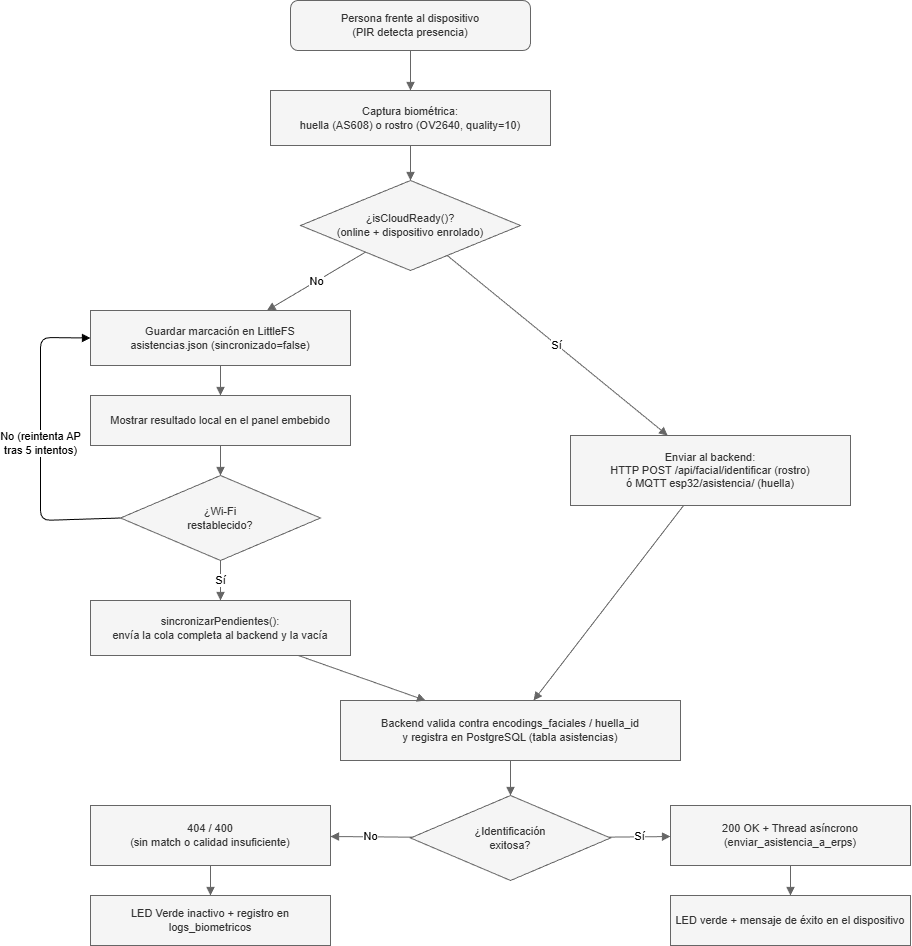
\includegraphics[width=.85\linewidth]{Imagenes/flujo_operacional_asistencia.png}
    \caption{Flujo operacional consolidado para el registro de asistencia.}
    \label{fig:flujo_operacional}
\end{figure}

\subsubsection{Pruebas}
\label{sec:pruebas_unitarias_automatizadas}

Se diseñaron las siguientes pruebas para validar la sincronización diferida, los logs y la integración final:

\begin{itemize}
    \item \textbf{Prueba de sincronización de asistencias offline}: Desconectar el ESP32-CAM de la red, registrar 5 marcaciones de entrada/salida para 2 personas diferentes, reconectar y ejecutar sincronización. Verificar que los 5 registros aparezcan en la base de datos del backend y que el archivo asistencias.json local los marque como sincronizados.

    \item \textbf{Prueba de idempotencia de sincronización}: Tras una sincronización exitosa, ejecutar nuevamente la sincronización sin nuevos registros. Verificar que no se inserten registros duplicados en el backend.

    \item \textbf{Prueba de sincronización de personas creadas offline}: Desconectar el dispositivo, registrar una nueva persona (con huella y datos), reconectar y sincronizar. Verificar que la persona aparezca en el backend con un ID definitivo (no local-).

    \item \textbf{Prueba de sincronización de turnos y asignaciones}: Desconectar el dispositivo, crear un turno y asignarlo a una persona existente, reconectar y sincronizar. Verificar que el turno y la asignación se repliquen en el backend y que los backend\_id locales se actualicen correctamente.

    \item \textbf{Prueba de persistencia tras corte de energía}: Durante una sincronización en curso, cortar la alimentación del ESP32-CAM. Al reiniciar, verificar que los archivos JSON no estén corruptos y que los registros con sincronizado = false sigan estando disponibles para una nueva sincronización.

    \item \textbf{Prueba de duplicados por turno}: Registrar dos asistencias con la misma persona, tipo, turno y fecha. Verificar que el sistema rechace la segunda inserción por duplicado. Registrar asistencias con diferentes turno\_id para un mismo día y verificar que ambas se registren sin conflictos.

    \item \textbf{Prueba de colación en turnos}: Crear un turno con colación habilitada (con\_colación = true) especificando horario de colación. Verificar que los campos colacion\_inicio y colacion\_fin se almacenen correctamente como TIME en la base de datos. Crear un turno sin colación y verificar que ambos campos sean NULL.

    \item \textbf{Prueba de logs de sincronización}: Ejecutar 3 sincronizaciones con diferentes cantidades de registros. Verificar que en la tabla sincronizacion\_log del backend aparezcan 3 entradas con los conteos correctos de registros enviados y procesados.

    \item \textbf{Prueba de logs biométricos}: Realizar operaciones de registro facial, identificación exitosa, identificación fallida y verificación. Verificar que cada operación genere una entrada en logs\_biometricos con el tipo de operación y resultado correctos.

    \item \textbf{Prueba de watchdog}: Iniciar el backend, verificar que todos los dispositivos se marquen como inactivos. Conectar un ESP32-CAM, verificar que tras el primer heartbeat cambie a activo. Desconectar el ESP32-CAM y verificar que tras 90 segundos el watchdog lo marque como inactivo.

    \item \textbf{Prueba de ping activo}: Conectar un ESP32-CAM, verificar que el backend publique pings en esp32/ping/<MAC> y que el dispositivo responda. Detener el ESP32-CAM (corte de red) y verificar que el ping activo marque el dispositivo como inactivo antes de que el watchdog de 90 segundos actúe (tiempo de espera de 60 segundos).

    \item \textbf{Prueba de simulación facial automatizada}: Utilizar la suite de pruebas test\_routes\_facial.py y el emulador test\_identificacion\_facial.py para simular el flujo completo de identificación 1:N con imágenes sintéticas generadas en memoria, cubriendo casos de coincidencia exitosa, rostro no registrado y calidad insuficiente de imagen.

    \item \textbf{Prueba de flujo completo punta a punta}: Ejecutar el flujo completo: registrar persona con huella y rostro en el ESP32-CAM $\rightarrow$ sincronizar con backend $\rightarrow$ verificar que la persona aparezca en el panel web $\rightarrow$ marcar asistencia por huella offline $\rightarrow$ reconectar y sincronizar $\rightarrow$ verificar que la asistencia aparezca en el panel web y se envíe al ERP de prueba.
\end{itemize}

\paragraph{Pruebas automatizadas}

Además de las pruebas funcionales descritas, se implementó una suite de más de 590 pruebas automatizadas para el backend y el firmware, utilizando pytest con PostgreSQL en Docker y mocks para DeepFace, OpenCV y MQTT. La suite se organiza en 35 archivos de prueba y alcanza una cobertura de código del 98\% sobre el código de producción del backend, sin fallos en ninguna de las pruebas (ver Anexo D para el detalle de casos y la evolución de la cobertura por módulo). La integración con los ERP externos se valida en dos niveles: por un lado, las pruebas de la suite automatizada cubren la creación, edición y prueba de webhooks de una integración ERP, simulando la respuesta del servidor externo. Por otro lado, dentro del subdirectorio ERPSIMULATORS/ se construyeron tres simuladores independientes (mock\_odoo.py, mock\_defontana.py y mock\_buk.py), cada uno levantando un pequeño servidor Flask que reproduce los endpoints reales de autenticación, consulta de empleados e inyección de marcaciones de su respectivo ERP comercial, según la documentación pública de cada proveedor. El script test\_erp\_mocks.py se ejecuta por separado, con los tres simuladores corriendo: envía una marcación con el formato que genera el sistema hacia cada uno de los tres mocks y verifica que el field mapping configurado para cada ERP transforme correctamente los datos y que cada simulador responda como lo haría el sistema real, imprimiendo un reporte de éxito o falla por caso. Esta validación manual complementa, sin sustituir, a las pruebas automatizadas de pytest.

Las pruebas cubren los flujos de todas las iteraciones: inicialización de la aplicación, esquema de base de datos, cifrado de embeddings, servicio de correo electrónico (con mock de SMTP), handlers MQTT, autenticación JWT con roles jerárquicos y flujo multi-empresa, endpoints faciales, CRUD de personas/turnos/asignaciones/asistencias, verificación de dispositivos, integraciones ERP con tolerancia a fallos de conexión y timeout, enrolamiento de dispositivos mediante PIN, sincronización offline, y logs de auditoría. Entre los módulos con mayor cobertura destacan el cifrado de embeddings (100\%), el servicio de correo (100\%), la gestión de turnos (100\%), la base de datos (99\%) y el módulo de asignaciones (96\%). El detalle completo de los casos de prueba se incluye en el Anexo D, que además resume los resultados obtenidos al ejecutar la suite completa.

\subsubsection{Refinamientos posteriores}

\begin{itemize}
    \item \textbf{Limpieza de datos al eliminar una persona}: el endpoint de eliminación distingue dos comportamientos según el rol de quien lo invoca. Un administrador ejecuta una limpieza completa de datos biométricos y sensibles: anonimiza el RUT, el correo y el identificador de huella, elimina los encodings\_faciales y los consentimientos asociados, borra la foto de previsualización del disco y marca a la persona como inactiva, conservando únicamente su historial de asistencias. Un empleador, en cambio, solo puede marcar a la persona como inactiva, sin acceso a la limpieza de datos biométricos, reservada al rol con mayor privilegio.

    \item \textbf{Filtro activo = true en los listados}: todas las consultas de lectura sobre personas (y entidades equivalentes) incorporan la condición WHERE activo = true, de modo que los registros eliminados mediante soft-delete dejan de aparecer en listados y búsquedas sin perder su información histórica en la base de datos, requisito necesario para mantener la integridad de los reportes de asistencia ya generados.
\end{itemize}


\section{Mecanismos de seguridad}

Esta sección consolida los mecanismos de seguridad implementados a lo largo de las distintas iteraciones, descritos en su momento dentro del desarrollo de cada una (Secciones 4.2.3 a 4.2.5), agrupándolos por capa: autenticación y control de acceso, enrolamiento de dispositivos, y protección de datos biométricos.

\subsection{Autenticación y control de acceso}

El backend define tres decoradores de autenticación en routes/auth.py, aplicados según el tipo de cliente que consume cada endpoint:

\begin{itemize}
    \item @token\_required: exige un header Authorization: Bearer <token> con un JWT firmado con el algoritmo HS256 y una clave secreta (JWT\_SECRET, configurable por variable de entorno). El token incluye user\_id, empresa\_id, rol y, opcionalmente, persona\_id, con una expiración de 24 horas. Si el token falta, está expirado o es inválido, el endpoint responde con HTTP 401.

    \item @requiere\_rol(*roles): envuelve a @token\_required y además exige que request.user\_rol esté dentro de los roles permitidos (admin, empleador o trabajador), respondiendo HTTP 403 en caso contrario. Implementa así un control de acceso jerárquico basado en roles sobre los mismos endpoints autenticados.

    \item @token\_opcional: permite que un mismo endpoint sea consumido tanto por un cliente web autenticado con JWT como por un dispositivo ESP32-CAM identificado mediante el header X-Device-MAC. Si no hay JWT, el decorador busca la MAC recibida entre los dispositivos ya enrolados y, de encontrarla, expone request.dispositivo\_id y request.empresa\_id para el resto del endpoint. Como se detalla en la Sección 4.2.5, este decorador ya no crea dispositivos nuevos automáticamente: solo vincula los que ya pasaron por el flujo de enrolamiento con PIN.

    \item @requiere\_dispositivo\_enrolado: complementa a @token\_opcional en endpoints biométricos sensibles (por ejemplo, /api/facial/registrar), verificando explícitamente que el dispositivo de la petición tenga enrolado = TRUE en la base de datos antes de continuar, y respondiendo HTTP 403 en caso contrario.
\end{itemize}

Las contraseñas de los usuarios del panel web nunca se almacenan en texto plano: se procesan con bcrypt \cite{bcrypt_pypi} (función hashpw con sal generada por gensalt()) tanto al crear una cuenta como al cambiar la contraseña, y la verificación en el login usa bcrypt.checkpw para comparar contra el hash almacenado.

\subsection{Enrolamiento seguro de dispositivos}

Un dispositivo ESP32-CAM no puede operar contra el backend simplemente conectándose a la red: debe pasar por un flujo de enrolamiento explícito basado en un PIN de un solo uso. Un administrador o empleador solicita POST /api/auth/dispositivos/generar-pin, que crea en la base de datos un registro en dispositivos con enrolado = FALSE y un código aleatorio de 8 caracteres alfanuméricos (generado con el módulo secrets, criptográficamente seguro). El dispositivo, desde su panel de configuración Wi-Fi, envía ese PIN junto con su dirección MAC al backend; si el PIN es válido y no fue usado antes, el dispositivo queda marcado como enrolado = TRUE y asociado a la MAC y a la empresa que generó el PIN. Un PIN ya consumido no puede reutilizarse (HTTP 409).

En el firmware, la función isCloudReady() (Sección 4.2.1) actúa como una verificación de doble factor antes de cualquier operación dependiente del backend: exige tanto conectividad de red (isOnline) como enrolamiento confirmado (estaEnrolado), evitando que un dispositivo conectado pero no autorizado, o autorizado pero sin red, ejecute operaciones que comprometerían la consistencia del sistema.

\subsection{Protección de datos biométricos}

Los embeddings faciales generados por DeepFace se cifran antes de almacenarse en la base de datos mediante Fernet (AES-128 en modo CBC con autenticación HMAC-SHA256), de la librería cryptography de Python. La clave de cifrado no se almacena directamente: se deriva aplicando SHA-256 a una variable de entorno (BIOMETRIC\_KEY) y codificando el resultado en base64 URL-safe, tal como lo exige la API de Fernet:

\begin{verbatim}
def _derivar_fernet_key() -> bytes:
    digest = hashlib.sha256(BIOMETRIC_KEY.encode("utf-8")).digest()
    return base64.urlsafe_b64encode(digest)
\end{verbatim}

De esta forma, ni el embedding ni la clave de cifrado quedan expuestos en texto plano en la base de datos: un acceso no autorizado a las tablas encodings\_faciales solo expone valores cifrados, mientras la clave reside exclusivamente en la configuración del entorno de ejecución del backend.

\section{Arquitectura de tiempo real (SSE)}

El panel web necesita reflejar, sin recargar la página, el estado de conexión de cada ESP32-CAM y el progreso del enrolamiento de huellas. Esta sección consolida cómo se implementó esa capa de tiempo real, descrita parcialmente al introducirse en las iteraciones 3 y 7 (Secciones 4.2.3 y 4.2.5).

\subsection{Endpoints de streaming}

El backend expone dos endpoints SSE (Server-Sent Events) implementados en app.py con el patrón estándar de Flask para streaming: una función generadora que produce eventos en formato text/event-stream, devuelta mediante Response(stream\_with\_context(generate()), mimetype='text/event-stream').

\begin{itemize}
    \item GET /sse/devices: difunde, a todos los clientes conectados, los cambios de estado de los dispositivos (heartbeat recibido, LWT disparado, ping sin respuesta), mediante la función broadcast\_device\_update().
    \item GET /sse/huellas: difunde el resultado del enrolamiento de huellas recibido por MQTT en esp32/huella/resultado/\#, mediante broadcast\_huella\_update(), permitiendo que el panel muestre en vivo el progreso del registro biométrico.
\end{itemize}

Se optó por SSE porque el caso de uso es unidireccional (servidor a cliente) y se consume en el navegador con la API nativa EventSource, sin depender de librerías adicionales en el frontend ni de un protocolo de negociación propio como el de WebSockets.

\subsection{Tres capas de detección de desconexión}

Determinar si un ESP32-CAM sigue conectado es más complejo que solo esperar sus heartbeats, porque una caída de red puede impedir que el dispositivo avise que se desconectó. El backend combina tres mecanismos complementarios, implementados en mqtt\_handler.py:

\begin{enumerate}
    \item \textbf{LWT (Last Will and Testament)}: al conectarse al broker MQTT, el ESP32-CAM registra un mensaje LWT en esp32/lwt/<MAC>. Si la conexión TCP se rompe de forma anómala (corte de energía, pérdida abrupta de señal), el propio broker Mosquitto publica ese mensaje automáticamente, sin que el backend tenga que esperar ningún timeout. Es la capa más rápida, pero depende de que el broker detecte la caída de la conexión subyacente.

    \item \textbf{Ping activo (device\_pinger)}: un hilo en segundo plano publica, cada 30 segundos, un mensaje en esp32/ping/<MAC> para cada dispositivo enrolado. El ESP32-CAM responde con un heartbeat normal al recibirlo. Si un dispositivo no responde dentro de la ventana definida por HEARTBEAT\_TIMEOUT (60 segundos), el pinger lo marca como inactivo directamente, sin esperar al watchdog. Esta capa cubre los casos en que el LWT no llega a publicarse (por ejemplo, si el broker tampoco detecta la caída).

    \item \textbf{Watchdog pasivo (device\_watchdog)}: un segundo hilo revisa cada 60 segundos la antigüedad del último heartbeat de cada dispositivo y marca como inactivos a los que superan los 60 segundos sin responder. Actúa como respaldo final, independiente del pinger, y además ejecuta un barrido inicial al arrancar el backend que marca a todos los dispositivos como inactivos hasta recibir su primer heartbeat.
\end{enumerate}

Cada vez que cualquiera de estas tres capas cambia el estado de un dispositivo en la base de datos, invoca broadcast\_device\_update(), que propaga el cambio de inmediato a los clientes SSE conectados.

\subsection{Consumo en el frontend}

En el panel web (Next.js), un hook personalizado se conecta directamente al endpoint /sse/devices mediante EventSource, actualizando en memoria el estado, IP y último heartbeat de cada dispositivo a medida que llegan eventos, sin necesidad de refrescar la página ni de mantener una conexión WebSocket. Como mecanismo de respaldo ante una eventual interrupción de la conexión SSE, el frontend además consulta periódicamente GET /api/dispositivos por REST, de modo que el estado mostrado no depende exclusivamente del canal de streaming.

\section{Prototipo final}
\label{sec:prototipo_final}

Esta sección presenta el resultado físico del proceso de desarrollo descrito en las ocho iteraciones anteriores, mostrando el dispositivo ESP32-CAM ensamblado junto con sus componentes periféricos (cámara OV2640, lector de huellas AS608 y sensor PIR), así como el panel web resultante.

%% Reemplazar por las fotografías reales del prototipo final.
%% Se recomienda incluir: (1) vista general del dispositivo ensamblado,
%% (2) detalle de conexiones/componentes, (3) dispositivo en su carcasa/montaje final,
%% (4) captura del panel web administrativo en funcionamiento.

\begin{figure}[H]
  \centering
  \includegraphics[width=0.75\linewidth]{Imagenes/prototipo_final_1.jpg}
  \caption{Vista general del prototipo final ensamblado.}
  \label{fig:prototipo_final_1}
\end{figure}

\begin{figure}[H]
  \centering
  \includegraphics[width=0.75\linewidth]{Imagenes/prototipo_final_2.jpg}
  \caption{Detalle de los componentes del prototipo: cámara OV2640, lector de huellas AS608 y sensor PIR.}
  \label{fig:prototipo_final_2}
\end{figure}

\begin{figure}[H]
  \centering
  \includegraphics[width=0.75\linewidth]{Imagenes/prototipo_final_3.jpg}
  \caption{Prototipo final montado en su carcasa definitiva.}
  \label{fig:prototipo_final_3}
\end{figure}

\begin{figure}[H]
  \centering
  \includegraphics[width=0.9\linewidth]{Imagenes/prototipo_final_4.jpg}
  \caption{Panel web administrativo en funcionamiento durante una prueba de campo.}
  \label{fig:prototipo_final_4}
\end{figure}

%% ============================================================
\section{Resumen del capítulo}
El capítulo 4 presenta el desarrollo completo del prototipo a lo largo de ocho iteraciones, siguiendo la metodología de prototipado evolutivo incremental. Se documenta la integración del hardware (ESP32-CAM, lector AS608, sensor PIR, cámara OV2640), la implementación del almacenamiento local con LittleFS y JSON, el desarrollo del backend con Flask y PostgreSQL (14 tablas con soporte multi-tenant), la comunicación mediante HTTP y MQTT, el reconocimiento facial con DeepFace (modelo Facenet, detector configurable MTCNN/RetinaFace y anti-spoofing), el cifrado de embeddings biométricos con Fernet, la autenticación JWT con roles jerárquicos, el enrolamiento seguro de dispositivos mediante PIN, el sistema antifraude multicapa (PIR + flash PWM + anti-spoofing + cooldown), el panel web para la gestión del dispositivo con streaming SSE de estado en tiempo real, la integración con ERP externos vía webhooks con field mapping, los mecanismos de sincronización diferida con logs de auditoría, y la detección de desconexión mediante un sistema de tres capas (LWT, ping activo y watchdog pasivo).

Cada iteración incluyó su respectivo análisis de requisitos, diseño de la solución, implementación detallada y un plan de pruebas de integración para validar el correcto funcionamiento de los componentes desarrollados. Adicionalmente, se documenta la suite de 591 pruebas unitarias automatizadas con pytest, que alcanzó una cobertura de código del 98\% sobre las 3.382 líneas de producción del backend, incluyendo pruebas de caja negra sobre los endpoints de la API REST y verificación exhaustiva de todos los caminos de error.

El Anexo C presenta, mediante diagramas de actividades, las principales funcionalidades implementadas en el sistema: el enrolamiento de dispositivos (Figura~\ref{fig:flujo_enrolamiento_dispositivo}), el registro de personas y captura biométrica (Figura~\ref{fig:flujo_registro_personas}), la gestión de turnos y su asignación (Figura~\ref{fig:flujo_gestion_turnos}), la sincronización diferida de asistencias pendientes (Figura~\ref{fig:flujo_sincronizacion_pendientes}) y el panel web administrativo (Figura~\ref{fig:flujo_panel_administrativo}). en memoria.tex
%% ============================================================

\chapter{Desarrollo e implementación}
En el siguiente capítulo se presentan en detalle las 8 iteraciones del proyecto, desarrolladas según la metodología de prototipado evolutivo incremental descrita en el capítulo 3. Para cada iteración se describen las fases de análisis, diseño, implementación y pruebas, reflejando la construcción progresiva del prototipo desde la integración inicial de hardware hasta la sincronización diferida y el cierre del proyecto.

\section{Diseño de software}
Esta sección está destinada a presentar las arquitecturas desarrolladas para este proyecto como así diagramas y mockups que permitan dar entender la lógica del proyecto como así futuras vistas.

\subsection{Arquitectura física}
La arquitectura física se organiza como un conjunto de servicios independientes que se comunican entre sí, siguiendo un enfoque de microservicios. La Fig.~\ref{fig:arq_fisica} muestra los componentes físicos involucrados y el camino que recorre una marcación desde que se genera hasta que queda disponible para la empresa: el ESP32-CAM, como dispositivo de campo, captura la imagen o la huella y la envía hacia el servidor mediante el broker MQTT (Mosquitto) o vía HTTP, según el tipo de operación. El backend (Flask) recibe esa información, invoca al servicio de reconocimiento facial (DeepFace) cuando corresponde, y persiste el resultado en la base de datos PostgreSQL. Desde ahí, el mismo backend se encarga de dos salidas independientes: reenviar la marcación al sistema ERP de la empresa mediante un webhook, y exponerla en el panel web (Next.js) para que el administrador o empleador la consulte en tiempo real.

\begin{figure}[H]
  \centering
  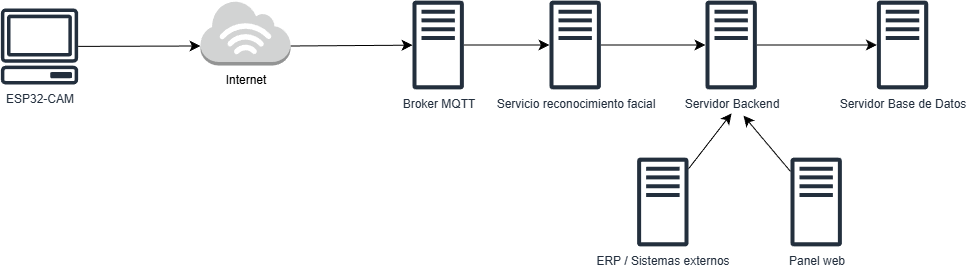
\includegraphics[width=\linewidth]{Imagenes/arqui2.drawio.png}
  \caption{Arquitectura física.}
  \label{fig:arq_fisica}
\end{figure}

\subsection{Arquitectura lógica}
Mientras que la arquitectura física muestra dónde corre cada servicio, la arquitectura lógica de la Fig.~\ref{fig:arq_logica} muestra cómo se organizan los módulos de software dentro de esos servicios y cómo se relacionan entre sí. En el lado del dispositivo, el ESP32-CAM agrupa cuatro módulos: la captura de imágenes (cámara OV2640), la lectura de huella (lector AS608 vía UART), el almacenamiento local en LittleFS (usuarios, turnos, asignaciones y asistencias en formato JSON) y el servidor web embebido que sirve la interfaz de configuración. Estos cuatro módulos no son independientes entre sí: por ejemplo, una marcación capturada por la cámara o el lector se guarda primero en LittleFS y solo después se intenta enviar al backend, lo que permite que el dispositivo siga funcionando aunque no haya conexión.

Del lado del servidor, el backend se organiza en blueprints de Flask (uno por dominio: personas, turnos, asistencias, dispositivos, ERP, etc.), cada uno con acceso a la base de datos PostgreSQL y, cuando corresponde, al servicio de reconocimiento facial. La comunicación entre el dispositivo y el backend ocurre por dos canales según el tipo de mensaje: MQTT para eventos de bajo volumen (heartbeats, comandos, resultados de enrolamiento) y HTTP para el envío de imágenes y la sincronización de datos. Esta separación de canales es la que permite que el dispositivo opere de forma autónoma cuando no hay red, almacene localmente lo que no pudo enviar, y sincronice todo una vez que la conexión se restablece.

\begin{figure}[H]
  \centering
  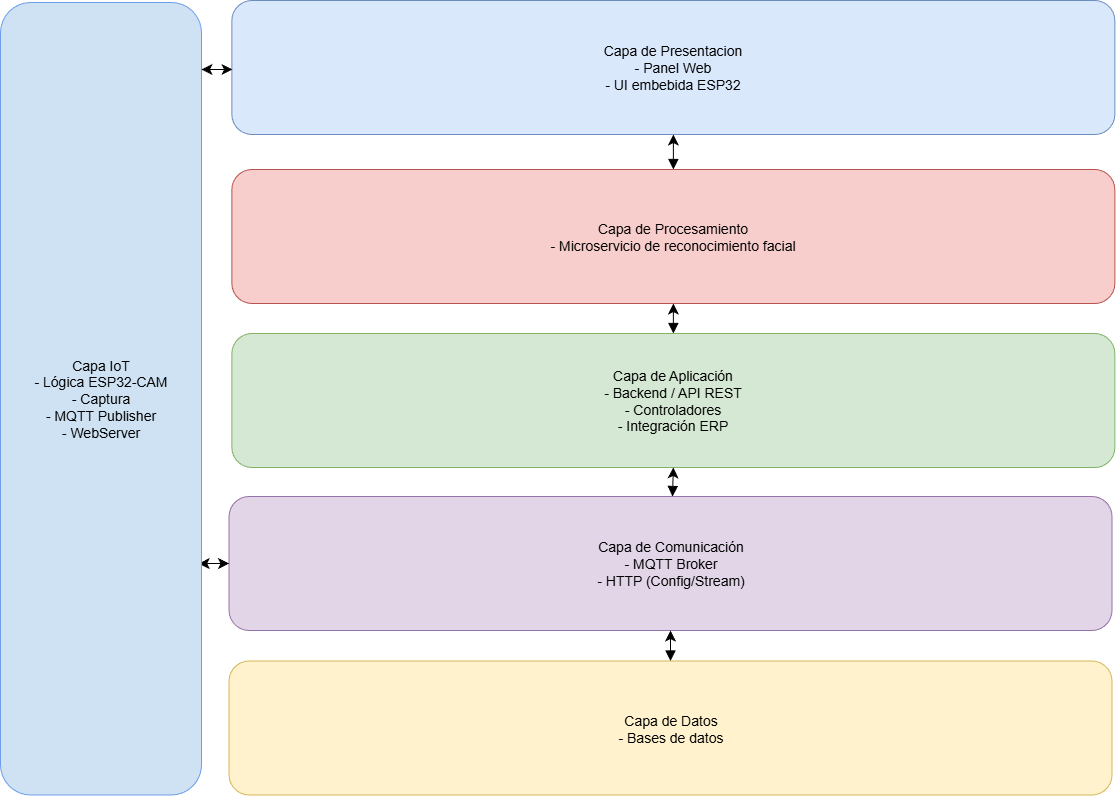
\includegraphics[width=.75\linewidth]{Imagenes/arquilogica.png}
  \caption{Arquitectura lógica.}
  \label{fig:arq_logica}
\end{figure}

La Fig.~\ref{fig:componentes_esp32} detalla, a nivel de hardware y firmware, los mismos cuatro módulos del ESP32-CAM descritos en la arquitectura lógica. En la capa de hardware se distinguen el microcontrolador ESP32, la cámara OV2640 (conectada por el bus paralelo DVP), el lector de huellas AS608 (conectado por UART) y el sensor PIR que activa la captura solo ante presencia detectada. En la capa de firmware, el servidor web embebido y el cliente MQTT comparten el acceso al sistema de archivos LittleFS, mientras que la máquina de estados central coordina cuándo se invoca cada módulo de captura biométrica según si el dispositivo está en modo de registro o de marcaje. Esta vista complementa a la Fig.~\ref{fig:arq_logica}, mostrando con qué pines y protocolos concretos se implementa cada bloque lógico.

\begin{figure}[H]
  \centering
  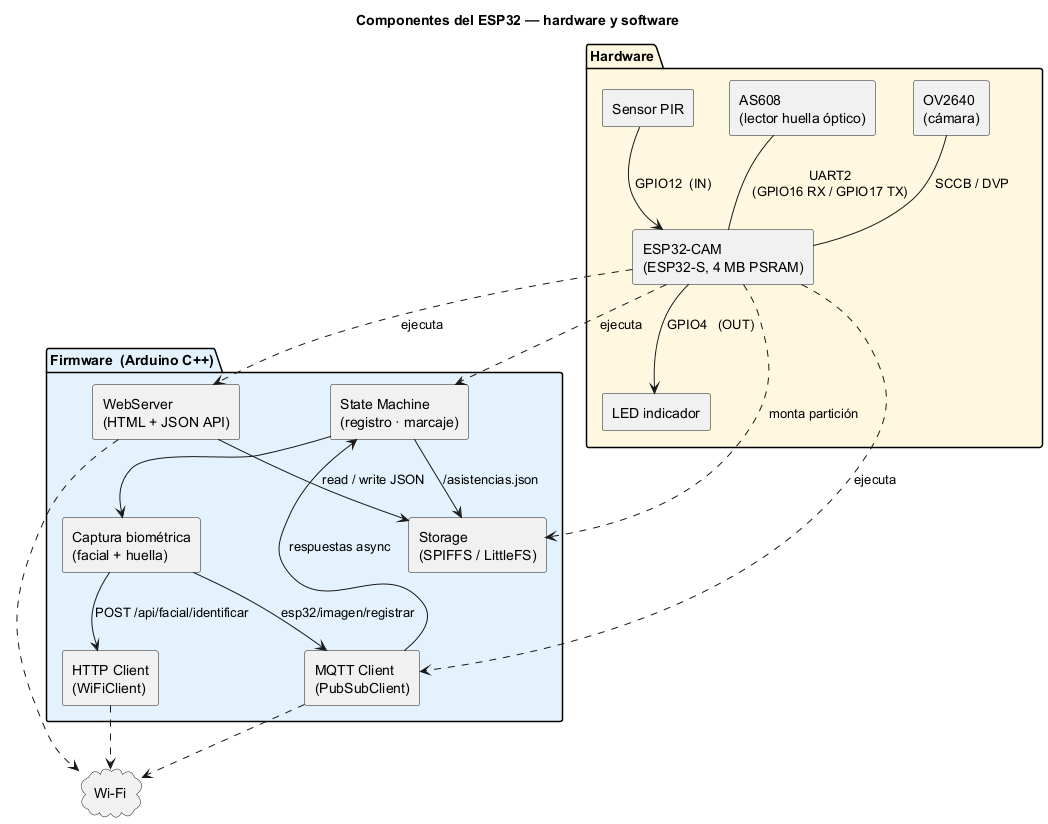
\includegraphics[width=\linewidth]{diagrams/componentes_esp32.png}
  \caption{Componentes del ESP32-CAM: hardware y firmware.}
  \label{fig:componentes_esp32}
\end{figure}

\section{Implementación}

En este apartado se procederá a explicar cómo se llevaron a cabo las iteraciones planteadas en el capítulo 3.1.

%% ============================================================
%% ITERACIÓN 1: Diseño y planificación inicial
%% ============================================================
\subsection{Iteración 1: Integración de hardware y servidor embebido}

La primera iteración corresponde al diseño conceptual del sistema y a la preparación del entorno de desarrollo, incluyendo la integración inicial del hardware biométrico seleccionado. Esta etapa establece la base funcional sobre la cual se construirán las iteraciones posteriores.

\subsubsection{Análisis}

En esta iteración se definieron los requisitos mínimos para validar la viabilidad técnica del sistema, analizando los componentes del hardware y las funcionalidades necesarias para las iteraciones siguientes.

El análisis se centró en tres ejes principales:

\begin{itemize}
    \item \textbf{Definición de funcionalidades mínimas (MVP)}:  
    Se identificaron las capacidades básicas que el dispositivo debía cumplir desde el inicio: capturar imágenes desde la cámara integrada, leer huellas dactilares mediante el sensor AS608, montar un servidor HTTP local con páginas HTML embebidas y operar de forma autónoma mediante Wi-Fi. Estas funciones representan la base operativa sobre la cual se desarrollarán características más avanzadas como turnos, sincronización y gestión de usuarios.

    \item \textbf{Identificación de limitaciones técnicas}:  
    Se revisaron las restricciones tecnológicas del ESP32-CAM, como la limitada memoria RAM disponible (~520 KB), el uso compartido del bus de cámara con los pines GPIO, la ausencia de pines GPIO libres -lo que forzó el uso de los pines GPIO14 (RX) y GPIO15 (TX) para la comunicación UART con el lector de huellas- y la necesidad de un manejo eficiente de cadenas HTML grandes en memoria. También se identificó que el flash LED integrado consume corriente significativa (~250 mA), requiriendo protección mediante PWM para evitar caídas de tensión durante la captura.

    \item \textbf{Estrategia de operación autónoma}:  
    Dado que uno de los requisitos fundamentales del sistema es la autonomía, se analizó la necesidad de montar un servidor web local. En caso de no contar con Wi-Fi configurada, el dispositivo debe activar automáticamente un modo Access Point (AP) con SSID ESP32-ASISTENCIA, permitiendo al administrador conectarse directamente para configurar la red y registrar usuarios sin dependencia de internet. Esto reduce riesgos y asegura la continuidad operacional del dispositivo.
\end{itemize}

Como resultado del análisis, se establecieron los criterios de diseño que guiarían el desarrollo de esta iteración: simplicidad, bajo consumo de recursos, modularidad de componentes y autonomía operativa.

\subsubsection{Diseño}

En esta iteración se elaboraron los primeros elementos arquitectónicos del sistema:

\begin{itemize}
    \item \textbf{Arquitectura física}, representando los componentes utilizados y su interconexión, la cual se puede revisar en la Fig.~\ref{fig:arq_fisica} de la sección 4.1.1.

    \item \textbf{Arquitectura lógica}, definiendo los módulos internos del firmware tales como captura de imágenes, lectura de huella, almacenamiento y conectividad, la cual se puede revisar en la Fig.~\ref{fig:arq_logica} de la sección 4.1.2.

    \item \textbf{Mockups iniciales} de la interfaz embebida del ESP32-CAM, incluyendo:

    \begin{itemize}
        \item Menú principal.
        \begin{figure}[H]
            \centering
            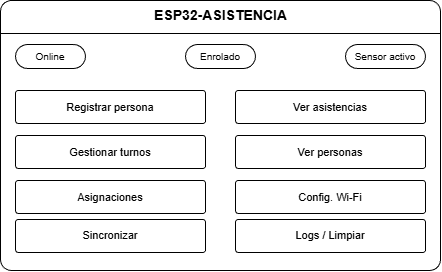
\includegraphics[width=.8\linewidth]{Imagenes/mockup_menu.png}
            \caption{Mockup menú principal en el ESP32-CAM.}
            \label{fig:mockup_menu}
        \end{figure}
        Wireframe inicial de la vista /: agrupa los indicadores de estado del dispositivo (conectividad, enrolamiento, sensor PIR) en la parte superior, y los accesos a cada módulo del sistema (registro, asistencias, turnos, personas, asignaciones, configuración Wi-Fi, sincronización y logs) como botones de navegación.

        \item Panel de configuración de Wi-Fi.
        \begin{figure}[H]
            \centering
            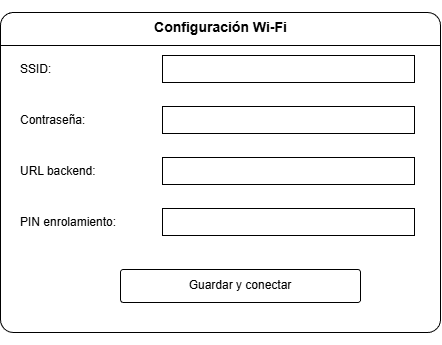
\includegraphics[width=.6\linewidth]{Imagenes/mockup_wifi.png}
            \caption{Mockup panel de configuración Wi-Fi.}
            \label{fig:mockup_wifi}
        \end{figure}
        Wireframe de la vista /wifi-setup: formulario con los cuatro campos que se persisten en wifi.json (SSID, contraseña de red, URL del backend y PIN de enrolamiento), accesible también desde el modo Access Point cuando el dispositivo no tiene credenciales configuradas.

        \item Vista de registro de usuario.
        \begin{figure}[H]
            \centering
            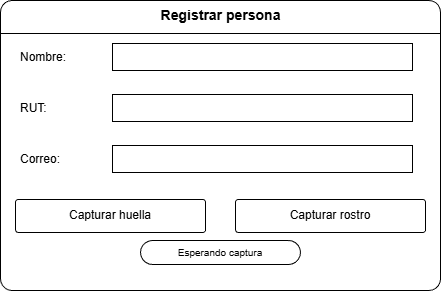
\includegraphics[width=.7\linewidth]{Imagenes/mockup_registro.png}
            \caption{Mockup registro de usuario en el ESP32-CAM.}
            \label{fig:mockup_registro}
        \end{figure}
        Wireframe de la vista /register: formulario de datos básicos (nombre, RUT, correo) seguido de los dos botones de captura biométrica, con un indicador de estado del proceso de enrolamiento (huella y rostro).

        \item Vista de usuarios almacenados localmente.
        \begin{figure}[H]
            \centering
            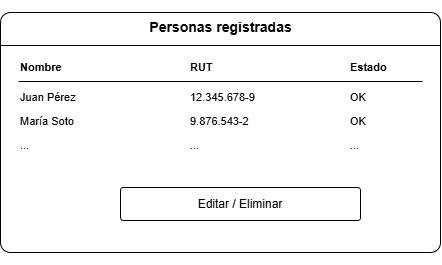
\includegraphics[width=.6\linewidth]{Imagenes/mockup_personas.png}
            \caption{Mockup de usuarios almacenados en el ESP32-CAM.}
            \label{fig:mockup_usuarios}
        \end{figure}
        Wireframe de la vista /personas: listado tabular de las personas registradas leídas desde personas.json, con acciones de edición y eliminación por fila.

        \item Vista de turnos almacenados localmente.
        \begin{figure}[H]
            \centering
            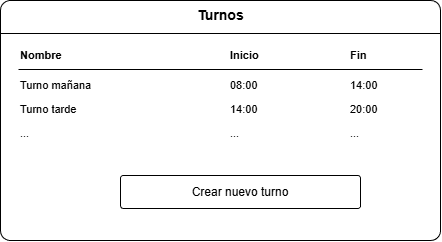
\includegraphics[width=.6\linewidth]{Imagenes/mockup_turnos.png}
            \caption{Mockup de visualización de turnos en el ESP32-CAM.}
            \label{fig:mockup_turnos}
        \end{figure}
        Wireframe de la vista /turnos: listado de los turnos almacenados en turnos.json, con el botón de acceso a la creación de un nuevo turno.

        \item Vista de crear turnos.
        \begin{figure}[H]
            \centering
            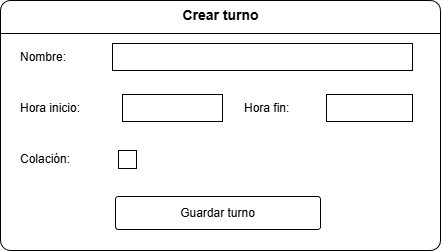
\includegraphics[width=.6\linewidth]{Imagenes/mockup_crear_turno.png}
            \caption{Mockup de creación de turnos en el ESP32-CAM.}
            \label{fig:mockup_crear_turnos}
        \end{figure}
        Wireframe de la vista /gestion: formulario para definir nombre, horario de inicio y fin, y la casilla opcional de colación que habilita los campos colacion\_inicio/colacion\_fin descritos en el Capítulo 4.

        \item Vista de asignación de turnos.
        \begin{figure}[H]
            \centering
            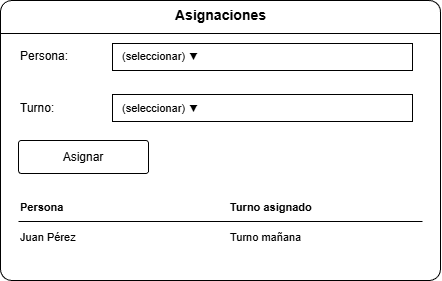
\includegraphics[width=.6\linewidth]{Imagenes/mockup_asignacion.png}
            \caption{Mockup de asignación de turnos en el ESP32-CAM.}
            \label{fig:mockup_asignacion}
        \end{figure}
        Wireframe de la vista /asignaciones: selección de persona y turno mediante listas desplegables, seguida del listado de asignaciones vigentes ya registradas.
    \end{itemize}

    \item \textbf{Diseño del flujo operacional}: a nivel conceptual, se planteó que el dispositivo debía capturar la huella o el rostro y luego evaluar si tenía conectividad disponible. Con conexión, la marcación se enviaría de inmediato al servidor; sin ella, se guardaría localmente para sincronizarse más adelante, cuando la red se restableciera. En ambos casos, la validación final (si la huella o el rostro corresponden a una persona registrada) ocurriría en el servidor, que respondería con un resultado de éxito o de error. El detalle de cómo se implementó cada uno de estos pasos, una vez que todos los componentes involucrados (enrolamiento, reconocimiento facial, sincronización diferida e integración ERP) estuvieron construidos, se presenta de forma consolidada al cierre del desarrollo, en la Sección~\ref{sec:flujo_operacional_consolidado}.
\end{itemize}

Estos elementos permiten visualizar el flujo básico del dispositivo antes de incorporar funcionalidades adicionales como turnos, sincronización o panel web backend, los cuales se desarrollarán en iteraciones posteriores.

\subsubsection{Implementación}

En esta etapa se integró tanto el hardware principal del prototipo como el desarrollo de las vistas web embebidas que permiten la interacción del usuario con el dispositivo. Para ello se utilizaron las siguientes librerías:

\begin{itemize}
    \item esp\_camera, utilizada para inicializar y configurar la cámara OV2640 integrada en el ESP32-CAM.
    \item HardwareSerial y Adafruit\_Fingerprint, empleadas para la comunicación UART con el lector biométrico AS608.
    \item WebServer, utilizada para montar un servidor web HTTP en el puerto 80 y atender rutas asociadas a las vistas.
    \item LittleFS y ArduinoJson \cite{arduinojson_docs}, empleadas para almacenamiento persistente en memoria flash y manipulación estructurada de datos JSON.
\end{itemize}

\paragraph{Integración del lector de huellas AS608}

El lector biométrico AS608 fue conectado directamente al ESP32-CAM mediante la interfaz UART secundaria (HardwareSerial 2), utilizando los pines GPIO14 (RX) y GPIO15 (TX). Esta conexión, que emplea pines distintos a los documentados inicialmente, fue forzada por la escasez de GPIO libres tras la asignación del bus de cámara. La velocidad de comunicación se estableció en 57600 baudios, y la librería Adafruit\_Fingerprint se vincula a dicho puerto serial. La Figura~\ref{fig:conexioneshuella} presenta la conexión física entre ambos dispositivos.

\begin{figure}[H]
    \centering
    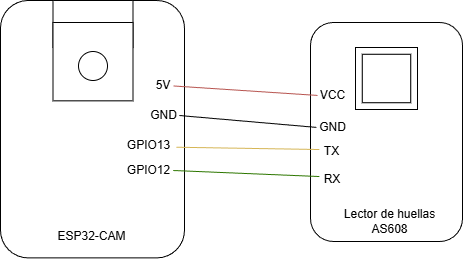
\includegraphics[width=.8\linewidth]{Imagenes/conexiones.png}
    \caption{Conexiones entre el ESP32-CAM y el lector de huellas AS608.}
    \label{fig:conexioneshuella}
\end{figure}

Una vez establecida la comunicación, el firmware puede ejecutar operaciones como:

\begin{itemize}
    \item Captura de imagen dactilar.
    \item Conversión de la imagen en una plantilla biométrica.
    \item Almacenamiento del template en un slot interno del sensor (1-127).
    \item Identificación mediante búsqueda de coincidencias en memoria.
\end{itemize}

La inicialización del lector se realiza con finger.begin(57600) sobre el puerto serie secundario, seguida de finger.verifyPassword() para confirmar que el sensor responde correctamente antes de habilitar las operaciones de captura, conversión y búsqueda descritas anteriormente.

\paragraph{Configuración de la cámara y el flash PWM}

La cámara OV2640 se configuró con resolución VGA (640×480) y compresión JPEG con calidad 8 (escala 0-63, donde valores bajos indican mayor calidad). La frecuencia del reloj externo (XCLK) se fijó en 20 MHz. Para evitar el parpadeo visible y las caídas de tensión provocadas por el flash LED durante la captura, se implementó un control PWM a 5 kHz con resolución de 8 bits, aplicando un ciclo de trabajo del 50\% (duty 128 de 255) durante la iluminación. Esto permite encender el flash con brillo suficiente sin sobrecargar la fuente de alimentación del ESP32-CAM.

\paragraph{Calibración del sensor PIR}

Se integró un sensor PIR (Passive Infrared) conectado al GPIO12 configurado con resistencia de pull-down interna. El sensor PIR actúa como detector de presencia: cuando una persona se sitúa frente al dispositivo, el PIR detecta el cambio de radiación infrarroja y activa el modo de captura. El setup incluye una fase de calibración de 3 segundos para estabilizar la lectura del sensor antes de iniciar el bucle principal. La lógica de uso del PIR como control de activación se detalla en la iteración 6.

\paragraph{Montaje del servidor web embebido}

Para habilitar la interacción local con el dispositivo, se implementó un servidor web mediante la librería WebServer en el puerto 80. Este servidor permite entregar páginas HTML, datos JSON y recursos estáticos. Cuando no hay conectividad a una red externa, el ESP32-CAM activa automáticamente un Access Point con SSID ESP32-ASISTENCIA y contraseña Asistencia2026, sirviendo las mismas páginas sin depender de internet.

Las rutas principales del sistema incluyen:

\begin{itemize}
    \item /: Menú principal con indicadores de estado.
    \item /wifi-setup: Configuración de red Wi-Fi y parámetros del backend.
    \item /register: Registro de personas con captura biométrica.
    \item /asistencias: Lista de asistencias almacenadas localmente.
    \item /gestion: Gestión de turnos (creación y administración).
    \item /personas: Visualización de personas registradas.
    \item /asignaciones: Vista para realizar asignaciones de turnos.
    \item /logs: Visualización de logs del sistema.
    \item /turnos: Visualización de turnos creados.
\end{itemize}

Para la implementación del servidor HTTP embebido, se utilizó el módulo WebServer del ESP32. Cada operación del sistema (registro de usuarios, captura de huellas, creación de turnos, asignación de turnos, lectura de asistencias, configuración Wi-Fi, entre otras) fue mapeada a un endpoint específico mediante funciones manejadoras (handler functions), registradas mediante "server.on(ruta, metodo, handler)" para cada una de las rutas listadas anteriormente. Este mecanismo permite encapsular la lógica de cada componente del sistema y mantener una estructura modular del firmware.

\paragraph{Creación de vistas HTML embebidas}

Las vistas fueron desarrolladas como archivos .html independientes almacenados en el sistema de archivos LittleFS del ESP32-CAM, conteniendo HTML, CSS y JavaScript autónomo, sin dependencias de CDN externas. El servidor web embebido las sirve mediante la función servirArchivo(), que lee el archivo solicitado desde LittleFS y lo envía al cliente. Esto garantiza que el ESP32-CAM sirva cada página incluso en modo Access Point sin conexión a internet.

\paragraph{Menú principal}

La Figura~\ref{fig:menu_principal} presenta la vista principal accesible en la ruta /. Desde esta interfaz el usuario puede visualizar el estado del dispositivo (online/offline, sensor activo, enrolado), registrar personas, ver asistencias, gestionar turnos, ver asignaciones, acceder a la configuración de red, sincronizar con el backend y limpiar datos del dispositivo. Con el avance de las iteraciones se agregaron a esta vista los indicadores de estado que se actualizan cada pocos segundos consultando al dispositivo, un bloque para mostrar el PIN de registro que permanece oculto hasta que el usuario decide revelarlo, una zona separada para las acciones de reinicio y borrado total de datos, y la opción de proteger la página con contraseña de administrador cuando se requiere restringir el acceso a esas acciones.

\begin{figure}[H]
    \centering
    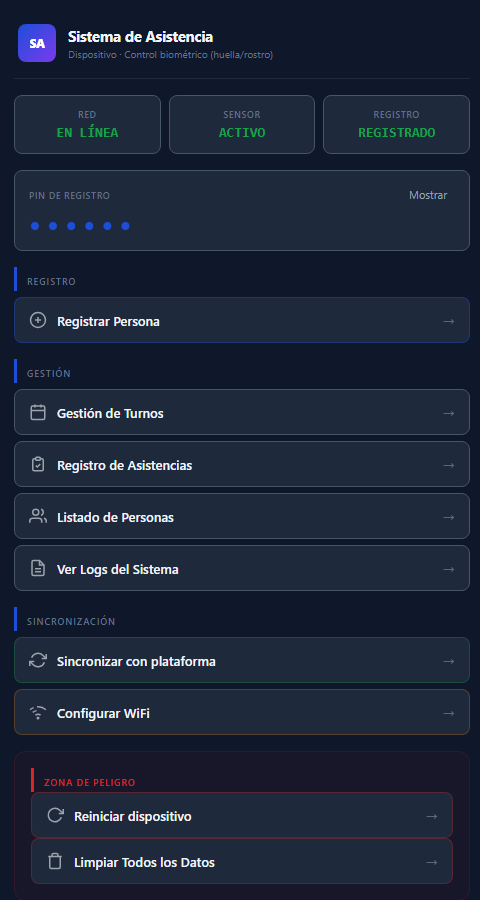
\includegraphics[height=8.5cm,keepaspectratio]{Imagenes/menuimplementado.png}
    \caption{Menú principal del sistema web embebido.}
\label{fig:menu_principal}
\end{figure}

\paragraph{Vista de configuración Wi-Fi}

Mediante la ruta /wifi-setup, el dispositivo proporciona un formulario para actualizar las credenciales de la red local (SSID, contraseña), la URL del backend, la dirección del broker MQTT y el PIN de enrolamiento. Estos valores se persisten en SPIFFS mediante el archivo wifi.json. La Figura~\ref{fig:wifi_config} muestra esta interfaz. Por requerimientos de seguridad identificados en iteraciones posteriores, se agregó a esta vista la opción de forzar conexiones cifradas hacia el backend y el broker MQTT, además de un apartado donde se puede definir o cambiar la contraseña de administrador pidiendo la contraseña actual como confirmación, de modo que no cualquier persona con acceso a la red local pueda modificar la configuración del dispositivo.

\begin{figure}[H]
    \centering
    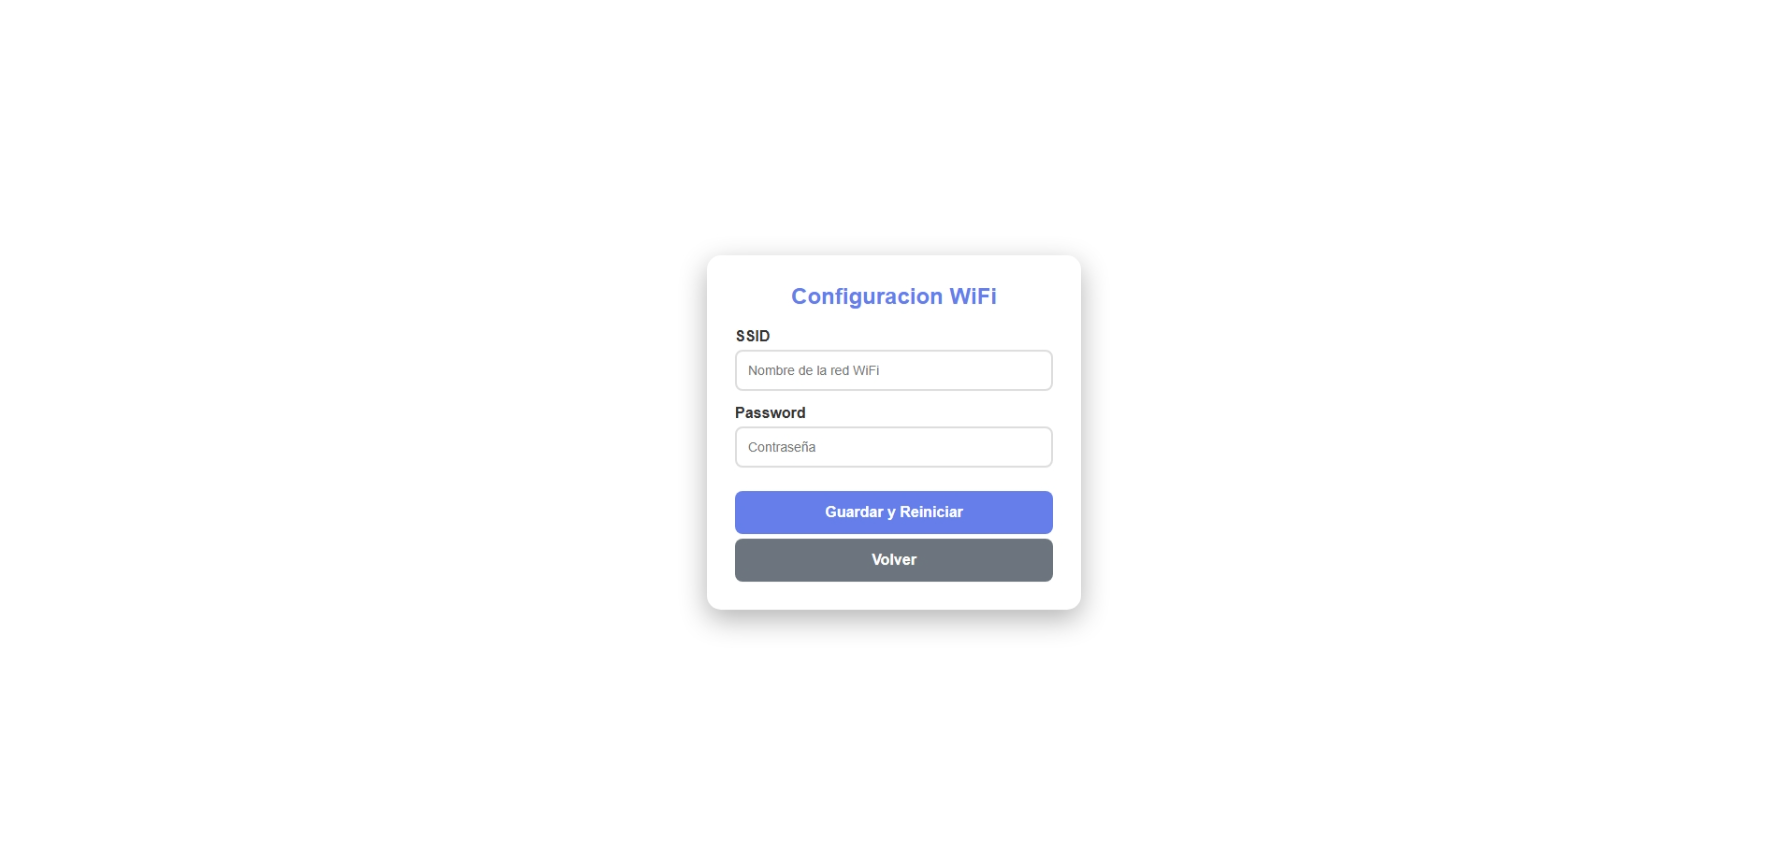
\includegraphics[height=8.5cm,keepaspectratio]{Imagenes/menuwifiimplementado.png}
    \caption{Interfaz de configuración Wi-Fi.}
\label{fig:wifi_config}
\end{figure}

\paragraph{Vista de registro de personas}

La ruta /register despliega una vista que combina un formulario para ingresar el nombre del usuario, RUT y correo electrónico, y muestra indicadores visuales del estado del proceso de enrolamiento (huella, rostro). La Figura~\ref{fig:registro_personas} lo muestra. Se incorporó a esta vista una casilla de consentimiento explícito para el tratamiento de datos biométricos, exigida por las consideraciones éticas y de privacidad descritas en el marco metodológico; mientras no se marque, el botón para iniciar el registro biométrico queda deshabilitado. El flujo se complementó además con un panel que informa el avance del proceso y con una pantalla de captura facial guiada, que muestra cuántas de las tres fotografías necesarias para el reconocimiento facial ya se han tomado.

\begin{figure}[H]
    \centering
    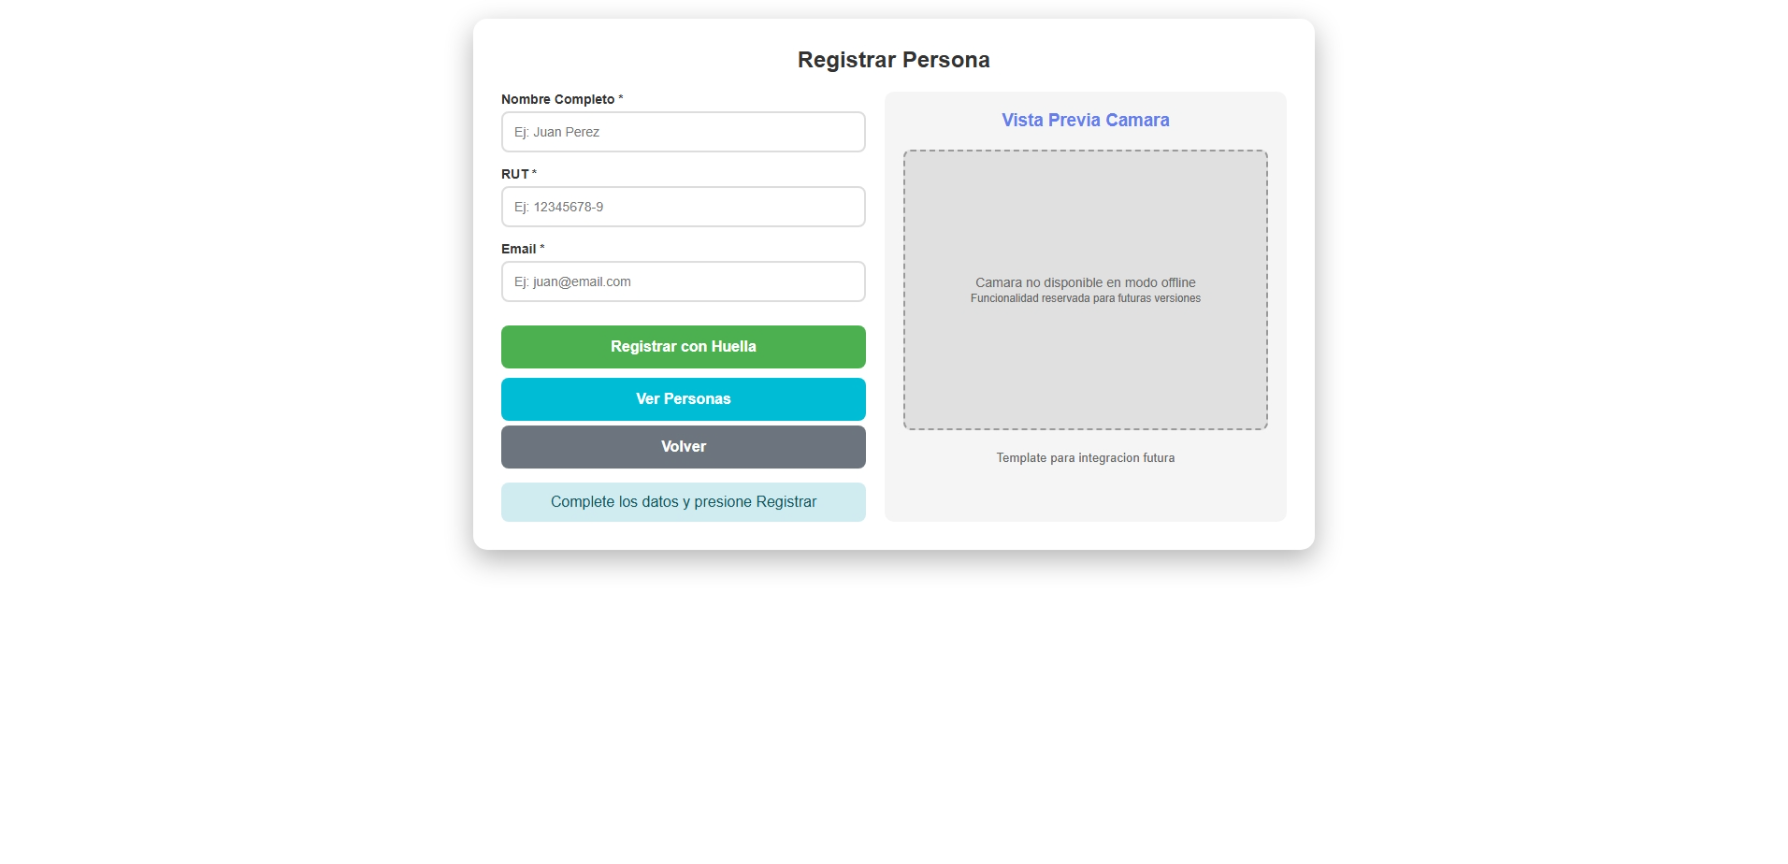
\includegraphics[height=8.5cm,keepaspectratio]{Imagenes/registroimplementado.png}
    \caption{Vista para el registro de personas en el dispositivo.}
\label{fig:registro_personas}
\end{figure}

\paragraph{Vista de asistencias}

Para visualizar registros de asistencia tanto locales como sincronizados, se implementó la vista en la ruta /asistencias. Esta consulta archivos JSON almacenados en LittleFS. La Figura~\ref{fig:vista_asistencias} lo ejemplifica. Cada registro se presenta como una tarjeta diferenciada por color según sea entrada o salida, con el nombre de la persona, la marca de tiempo y su identificador asociado. A la versión inicial, que solo listaba los registros, se le agregaron las opciones de editar o eliminar cada fila, pensadas para que el encargado de turno pueda corregir una marcación errónea, como una doble lectura biométrica, sin necesidad de acceder directamente al backend. También se sumó un contador de registros totales en la parte superior, útil para revisar de un vistazo cuántos datos hay almacenados localmente antes de sincronizar.

\begin{figure}[H]
    \centering
    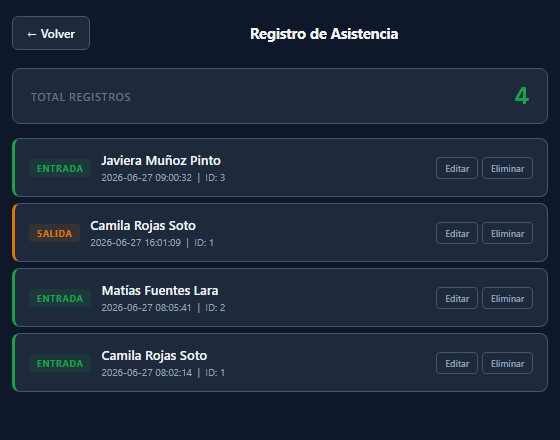
\includegraphics[height=8.5cm,keepaspectratio]{Imagenes/vistaasitenciasimplementado.png}
    \caption{Vista de asistencias locales almacenadas en el dispositivo.}
\label{fig:vista_asistencias}
\end{figure}

\paragraph{Vista de Personas registradas}

Para visualizar las personas registradas, se implementó la vista en la ruta /personas. Esta consulta archivos JSON almacenados en LittleFS y permite editar nombre/correo, actualizar huella o rostro, y eliminar personas. La Figura~\ref{fig:personas_registradas} lo ejemplifica. Las opciones para actualizar la huella o el rostro, y para agregar fotos adicionales, se incorporaron después de notar en las pruebas de campo que volver a registrar a una persona desde cero, borrando y repitiendo todo el proceso, tomaba demasiado tiempo. Con estas opciones se puede corregir solo la huella o el rostro de alguien ya registrado, o sumar fotos para mejorar el reconocimiento facial, sin perder el resto de sus datos ni su historial de asistencia.

\begin{figure}[H]
    \centering
    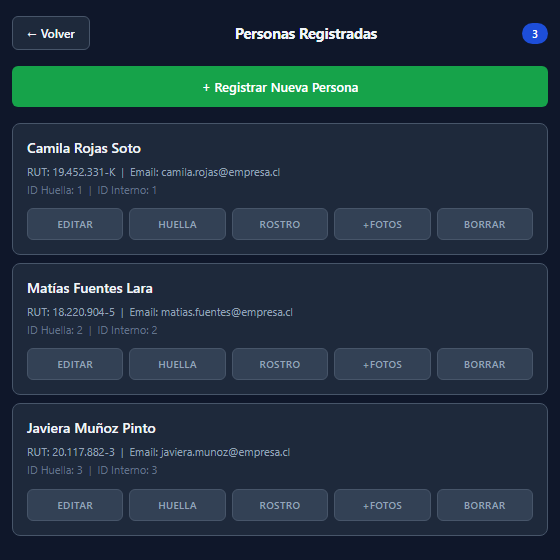
\includegraphics[height=8.5cm,keepaspectratio]{Imagenes/personasregistradasimplementada.png}
    \caption{Vista de personas registradas en el dispositivo.}
\label{fig:personas_registradas}
\end{figure}

\paragraph{Vista de Crear Turnos}

Para la creación de turnos y visualización de los existentes, se implementó la vista en la ruta /gestion, complementada con /turnos. Estas consultan archivos JSON almacenados en LittleFS. La Figura~\ref{fig:gestion_turnos} lo ejemplifica. La vista /gestion funciona como panel resumen, con accesos directos a la gestión de turnos, a las asignaciones y a la sincronización manual con la plataforma. La vista /turnos concentra el formulario para crear un turno nuevo, con nombre, hora de inicio y fin, y un selector de días de la semana, junto con el listado editable de los turnos ya creados. Esta separación entre resumen y edición se introdujo para que las modificaciones no ocurran por accidente desde la pantalla que se usa con más frecuencia.

\begin{figure}[H]
    \centering
    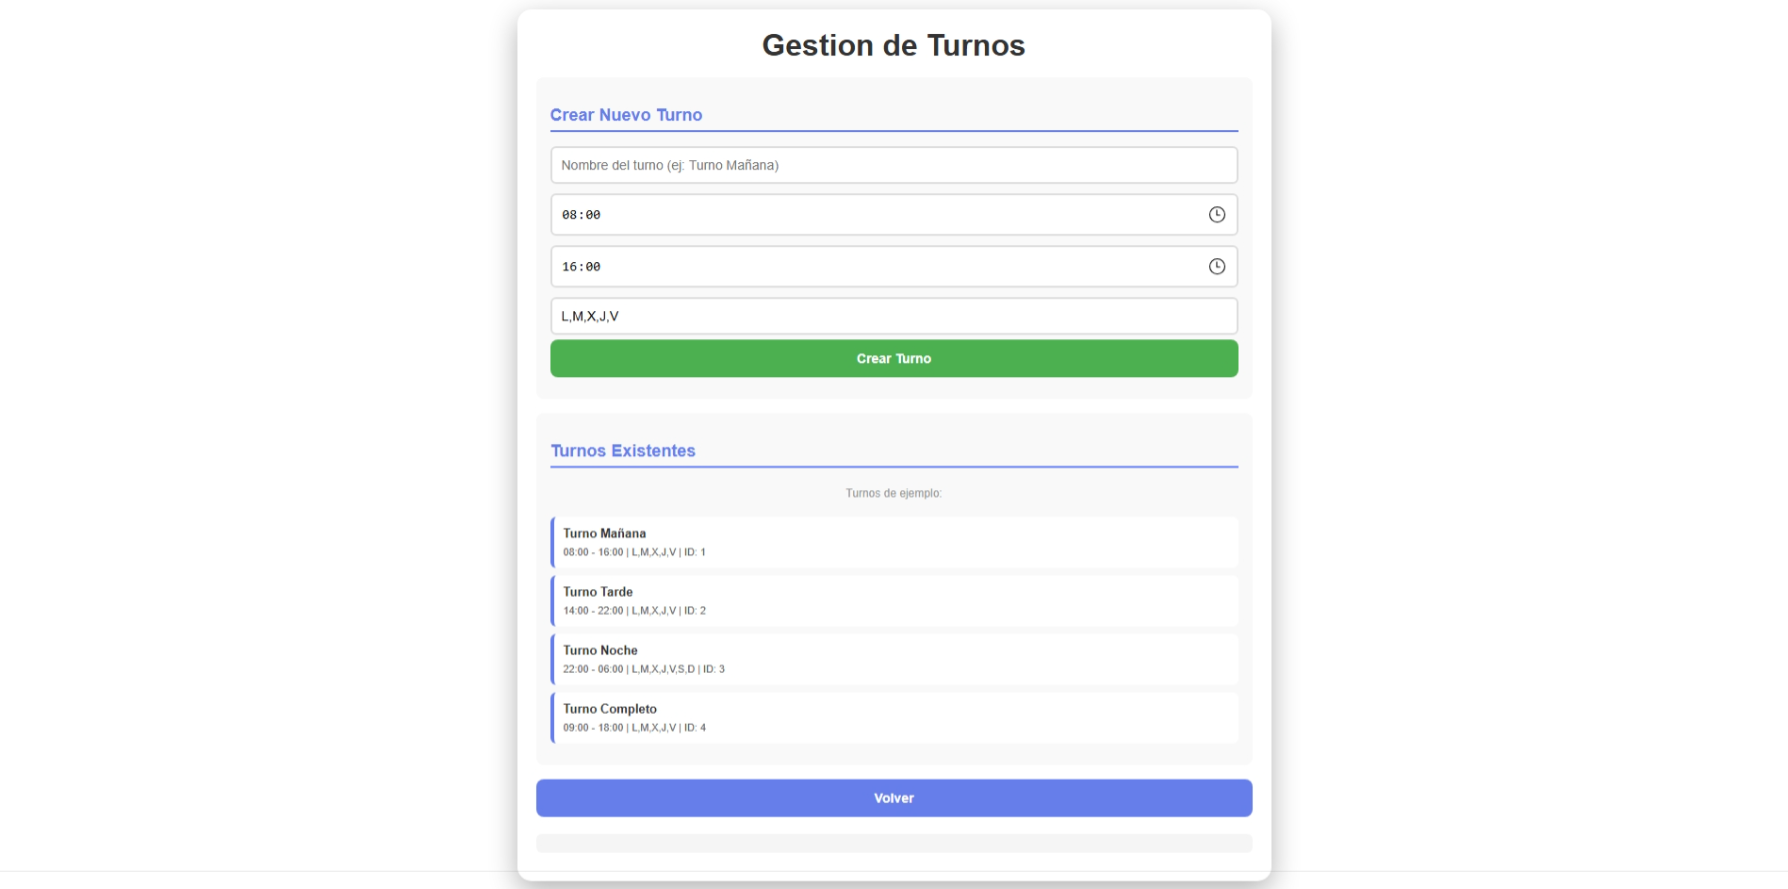
\includegraphics[height=8.5cm,keepaspectratio]{Imagenes/creacionturnos.png}
    \caption{Vista de gestión y creación de turnos en el dispositivo.}
\label{fig:gestion_turnos}
\end{figure}

\paragraph{Vista de asignación de turnos}

Para visualizar las asignaciones de turnos y realizar la acción de asignar un turno a una persona, se implementó la vista en la ruta /asignaciones. La Figura~\ref{fig:asignacion_turnos} lo ejemplifica. El formulario superior permite elegir una persona y un turno ya creados desde listas desplegables, evitando que el usuario tenga que recordar o escribir identificadores internos. El listado de asignaciones actuales muestra el nombre de la persona y del turno en lugar de solo sus identificadores, e incluye una opción para quitar una asignación, agregada después de notar que reasignar turnos por cambios de horario del personal era algo que ocurría seguido durante el uso del prototipo.

\begin{figure}[H]
    \centering
    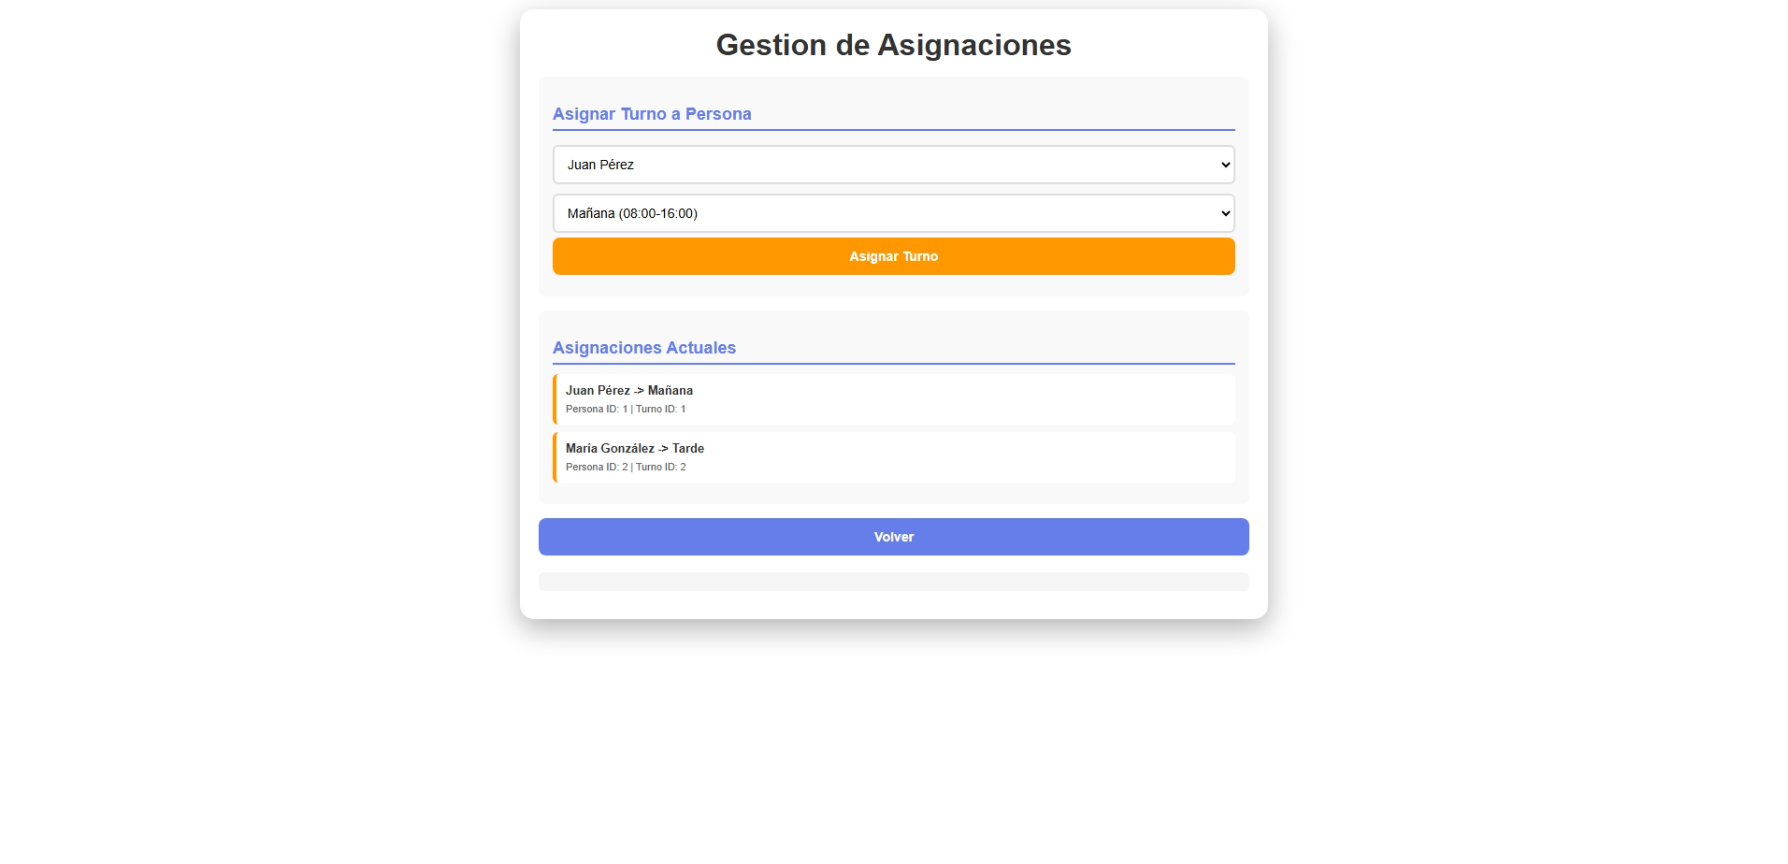
\includegraphics[height=8.5cm,keepaspectratio]{Imagenes/asignacionturnoimplementacion.png}
    \caption{Vista de gestión de asignaciones en el dispositivo.}
\label{fig:asignacion_turnos}
\end{figure}

\subsubsection{Pruebas}

Para validar el funcionamiento del prototipo y comprobar la correcta integración entre los distintos módulos del sistema, se diseñaron pruebas de integración enfocadas exclusivamente en los componentes implementados durante esta iteración:

\begin{itemize}
    \item \textbf{Prueba de captura de imágenes}: Verificar que la cámara OV2640 capture imágenes JPEG de forma continua y estable, sin corrupción de frames ni errores de inicialización del sensor. Se espera que la función esp\_camera\_fb\_get() retorne buffers consistentes tras cada llamada.

    \item \textbf{Prueba de comunicación UART con AS608}: Verificar que el lector biométrico responda correctamente al comando de verificación de contraseña (finger.verifyPassword()) y que la comunicación serie a 57600 baudios se establezca sin pérdida de paquetes. Se espera confirmación de conexión en menos de 1 segundo tras el inicio.

    \item \textbf{Prueba de lectura biométrica}: Verificar que el AS608 pueda capturar una imagen dactilar (finger.getImage()), convertirla a plantilla (finger.image2Tz()) y almacenarla en un slot del sensor (finger.storeModel()). Se espera que el proceso completo tome menos de 2 segundos.

    \item \textbf{Prueba de acceso vía AP}: Verificar que al iniciar sin credenciales Wi-Fi configuradas, el ESP32-CAM active el Access Point ESP32-ASISTENCIA y que las páginas HTML sean accesibles desde un navegador conectado a la IP 192.168.4.1. Se espera que todas las rutas definidas respondan con código HTTP 200.

    \item \textbf{Prueba de carga de vistas vía Wi-Fi externa}: Verificar que al conectar el dispositivo a una red Wi-Fi configurada, las mismas vistas se carguen correctamente a través de la IP asignada por el router, manteniendo estilos, scripts y funcionalidad.
\end{itemize}

\subsubsection{Refinamientos posteriores}

Durante el desarrollo de las iteraciones siguientes surgieron dos problemas asociados a la base construida en esta etapa, los cuales fueron corregidos durante el mismo ciclo de implementación.

El primero se presentó al combinar las funcionalidades de conectividad y enrolamiento: un dispositivo podía encontrarse conectado a internet sin contar aún con una persona enrolada, o bien tener una persona enrolada pero haber perdido la conexión de red. En ambos casos, el firmware intentaba ejecutar la sincronización o el reconocimiento facial de igual forma, lo que provocaba fallos sin generar un mensaje de error claro para el usuario. Para resolver esta situación, se implementó una función de validación que verifica simultáneamente ambas condiciones antes de permitir cualquier operación dependiente del backend, evitando así que el dispositivo ejecute procesos que se sabe resultarán en error.

El segundo ajuste estuvo relacionado con la calidad de las imágenes utilizadas para el reconocimiento facial. Las capturas estándar de la cámara se almacenaban con un nivel de compresión orientado a vistas previas rápidas, el cual resultaba insuficiente para generar un embedding facial de calidad adecuada, debido a la pérdida de detalle en los rasgos del rostro. Por este motivo, se diferenció el proceso de captura correspondiente al registro biométrico, incrementando temporalmente la resolución del sensor exclusivamente para la fotografía de referencia, y restableciéndola a su configuración estándar una vez completada la captura, sin afectar el resto de las imágenes procesadas por el sistema.

%% ============================================================
%% ITERACIÓN 2: Almacenamiento local y modo offline
%% ============================================================

\subsection{Iteración 2: Almacenamiento local y modo offline}

La segunda iteración se centra en habilitar el funcionamiento autónomo del dispositivo sin conexión a internet, integrando un sistema de almacenamiento persistente basado en LittleFS (sucesor moderno de SPIFFS para ESP32) y los mecanismos de captura biométrica offline. Esta etapa materializa lo definido en el apartado 3.1.2 del capítulo anterior.

\subsubsection{Análisis}

Para el correcto funcionamiento offline del prototipo se identificaron los siguientes requerimientos:

\begin{itemize}
    \item Almacenar localmente los datos de usuarios, turnos, asignaciones y asistencias en formato JSON.
    \item Permitir el registro de marcaciones aun cuando no exista conectividad externa, tanto por huella (offline total) como con validación de turnos locales.
    \item Garantizar persistencia de la información tras reinicios del ESP32-CAM o cortes de energía.
    \item Habilitar la gestión completa del sistema mediante una interfaz web embebida accesible vía Access Point.
    \item Mantener compatibilidad con la futura sincronización automática en modo online, marcando cada registro con un campo sincronizado (booleano) para su posterior envío al backend.
\end{itemize}

Para cumplir estos requisitos se seleccionó el sistema de archivos LittleFS y el formato JSON debido a su bajo peso, facilidad de manipulación mediante la librería ArduinoJson y compatibilidad con las capacidades del ESP32-CAM (4 MB de flash, de los cuales aproximadamente 1.5 MB están disponibles para LittleFS). Adicionalmente, se definió un archivo de configuración, wifi.json, destinado a almacenar credenciales Wi-Fi, URL del backend, dirección del broker MQTT y PIN de enrolamiento.

\subsubsection{Diseño}

Considerando la arquitectura establecida, se diseñaron las siguientes estructuras de almacenamiento en formato JSON:

\begin{itemize}
    \item \textbf{personas.json}: Arreglo de objetos con campos id, nombre, rut, email, huella\_id, fecha\_registro, sincronizado.
    \item \textbf{turnos.json}: Arreglo de objetos con campos id, backend\_id, nombre, inicio, fin, dias, sincronizado.
    \item \textbf{asignaciones.json}: Arreglo de objetos con campos persona\_id, turno\_id, backend\_id, fecha\_asignacion, sincronizado.
    \item \textbf{asistencias.json}: Arreglo de objetos con campos persona\_id, nombre, tipo (entrada/salida), metodo (huella\_offline, facial, etc.), timestamp, sincronizado.
    \item \textbf{wifi.json}: Objeto con campos ssid, pass, backend, mqtt, pin (para enrolamiento del dispositivo).
    \item \textbf{erp-config.json}: Arreglo con configuraciones de integraciones ERP, sincronizado desde el backend cuando hay conectividad.
\end{itemize}

El campo sincronizado (booleano) en cada entidad actúa como bandera para el proceso de sincronización diferida: cuando el dispositivo recupera conectividad, itera sobre los registros con sincronizado = false y los envía al backend. Una vez confirmada la recepción, se marca sincronizado = true.

\subsubsection{Implementación}

En esta iteración se integraron las librerías LittleFS, ArduinoJson, HardwareSerial y Adafruit\_Fingerprint. Las dos primeras permiten gestionar archivos JSON alojados en la memoria flash del ESP32-CAM, mientras que las dos últimas habilitan la comunicación UART con el lector biométrico AS608 para el registro y verificación de huellas digitales.

\paragraph{Inicialización del sistema de archivos y persistencia}

El primer componente de la implementación consiste en montar LittleFS mediante LittleFS.begin(true) y verificar la existencia de los archivos necesarios. En caso de no existir, el sistema los crea con una estructura inicial vacía (arreglo [] para las colecciones, objeto con valores por defecto para wifi.json), asegurando que el dispositivo pueda operar incluso tras un primer arranque sin configuración previa.

Se implementaron dos funciones genéricas para la manipulación de archivos JSON:

\begin{itemize}
    \item loadArray(const char* path, DynamicJsonDocument\& doc): Abre un archivo, deserializa su contenido como JsonArray y lo retorna. Si el archivo no existe o está corrupto, retorna un arreglo vacío.
    \item saveArray(const char* path, DynamicJsonDocument\& doc): Serializa el documento JSON y lo escribe en el archivo correspondiente, sobrescribiendo el contenido anterior.
\end{itemize}

Estas funciones encapsulan toda la lógica de persistencia del sistema y son reutilizadas por todos los módulos que necesiten leer o escribir datos.

El tamaño de cada DynamicJsonDocument se dimensionó según el volumen esperado de datos de cada archivo, aunque varía según la función que lo utiliza: asignaciones.json utiliza típicamente 1024~bytes, personas.json y turnos.json se manejan con buffers de entre 2048 y 8192~bytes dependiendo del contexto (lectura local, sincronización o registro), y asistencias.json utiliza 32768~bytes. Adicionalmente, en la función procesarAsistencia() se incorporó una validación sobre el retorno de createNestedObject(): si el objeto retornado es nulo (indicando desbordamiento del documento), se registra una advertencia en el log del sistema, permitiendo detectar tempranamente cuellos de botella de memoria sin comprometer la integridad del archivo JSON. El dimensionamiento de este buffer y la estrategia adoptada para sostener el volumen de registros exigido en los objetivos del proyecto se detallan en el apartado de refinamientos posteriores de esta iteración.

\paragraph{Registro de usuarios con huella digital}

El registro de usuarios se implementó mediante un flujo que combina la captura biométrica gestionada por el lector AS608 con el almacenamiento en personas.json. El lector administra internamente modelos de huellas mediante \textit{slots} numerados del 1 al 127. Por ello, antes del enrolamiento es necesario identificar un slot disponible dentro del sensor. La función encontrarSlotLibre() recorre el arreglo de personas, determina el ID de huella más alto registrado y retorna el siguiente disponible.

Una vez encontrado un slot, se ejecuta el proceso de enrolamiento en dos fases:

\begin{enumerate}
    \item \textbf{Primera captura} (ESTADO\_ESPERANDO\_HUELLA\_REGISTRO): El sistema espera que el usuario coloque el dedo. Al detectar una imagen válida, la convierte a plantilla en el buffer 1 y transiciona a ESTADO\_ESPERANDO\_SOLTAR\_DEDO.
    \item \textbf{Espera y segunda captura} (ESTADO\_REGISTRO\_SEGUNDA\_HUELLA): Una vez que el sensor detecta que el dedo fue retirado (FINGERPRINT\_NOFINGER), el sistema solicita una segunda captura del mismo dedo. Al obtenerla, convierte a plantilla en el buffer 2, crea el modelo combinado (finger.createModel()) y lo almacena en el slot correspondiente (finger.storeModel()).
\end{enumerate}

Luego del enrolamiento exitoso, se almacena un nuevo objeto dentro de personas.json con un identificador único (generado localmente con prefijo local- o provisto por el backend si hay conectividad), el nombre, RUT, correo electrónico y el slot asignado. La etapa de captura de huella aquí descrita corresponde a los primeros estados de la máquina de estados del registro biométrico completo, presentada más adelante en la Figura~\ref{fig:maquina_estados_esp32} (sección 4.3.4), una vez introducido el envío de la foto de referencia al backend por HTTP.

\paragraph{Registro de asistencia en modo offline}

El registro de asistencia se realiza completamente en el dispositivo, sin necesidad de conexión externa. El flujo implementado consiste en:

\begin{enumerate}
    \item Capturar una huella mediante el lector AS608 (finger.getImage()).
    \item Convertir la imagen a plantilla (finger.image2Tz()) y ejecutar una búsqueda biométrica (finger.fingerSearch()) que retorna el fingerID del slot coincidente.
    \item Identificar al usuario asociado mediante el campo huella\_id en personas.json con la función buscarPersonaPorHuella().
    \item Verificar que el usuario cuente con un turno asignado consultando asignaciones.json mediante turnoActivo(). Si no tiene turno, el sistema rechaza la marcación.
    \item Determinar el tipo de evento (entrada/salida) alternando automáticamente respecto al último registro de la persona en asistencias.json.
    \item Generar un nuevo registro con sincronizado = false (salvo que se logre enviar al backend en ese momento).
\end{enumerate}

El manejador handleMarcarAsistencia() expone esta funcionalidad a través de la interfaz web, permitiendo también marcaciones manuales. El escaneo automático continuo se controla mediante intervalos configurables: 2 segundos entre verificaciones de huella y 6 segundos entre verificaciones faciales.

\paragraph{Gestión de turnos y asignaciones}

Además del registro de asistencias, el sistema permite crear turnos (handleCreateTurn()) y asignarlos a personas (handleAssignTurn()) desde la interfaz web. Cada operación persiste los datos en sus archivos JSON correspondientes y, si hay conectividad, intenta replicar la operación en el backend mediante HTTP POST.

\paragraph{Operación offline del dispositivo}

Con el objetivo de asegurar autonomía total, el ESP32-CAM fue configurado para operar en dos modos:

\begin{itemize}
    \item \textbf{Modo Wi-Fi STA}: Si hay credenciales configuradas en wifi.json, el dispositivo intenta conectarse a la red externa. Si la conexión falla reiteradamente (5 intentos), activa el modo AP como fallback sin deshabilitar el intento de reconexión.
    \item \textbf{Modo Access Point}: El punto de acceso utiliza el SSID ESP32-ASISTENCIA y contraseña Asistencia2026, permitiendo que un administrador se conecte directamente al dispositivo en la IP 192.168.4.1 para realizar todas las operaciones mediante la interfaz web embebida.
\end{itemize}

\subsubsection{Pruebas}

Se diseñaron las siguientes pruebas para validar el correcto funcionamiento del almacenamiento local y el modo offline:

\begin{itemize}
    \item \textbf{Prueba de persistencia tras reinicio}: Registrar usuarios, turnos, asignaciones y asistencias, luego reiniciar el ESP32-CAM (por corte de energía o comando software). Verificar que todos los archivos JSON conserven su contenido íntegro y que el sistema pueda leerlos correctamente tras el reinicio.

    \item \textbf{Prueba de lectura y deserialización}: Abrir cada archivo JSON generado y verificar que ArduinoJson pueda deserializar su contenido sin errores ni pérdida de campos. El tamaño de cada DynamicJsonDocument se configuró según la capacidad esperada del archivo: 2048~bytes para personas.json y turnos.json, 1024~bytes para asignaciones.json y 32768~bytes para asistencias.json. Se incluyó además una validación post-inserción (mediante isNull()) en la función procesarAsistencia() para detectar y registrar en logs cualquier desbordamiento del documento al crear nuevos registros de asistencia.

    \item \textbf{Prueba de escritura concurrente}: Realizar múltiples operaciones de escritura (registro de persona + asignación de turno + marcación de asistencia) en rápida sucesión sin reiniciar el sistema. Verificar que no se produzcan corrupciones de archivos ni pérdida de datos.

    \item \textbf{Prueba de marcación offline por huella}: Desconectar el dispositivo de toda red externa, registrar un usuario con huella y turno, y efectuar una marcación. Verificar que el registro aparezca en asistencias.json con sincronizado = false.

    \item \textbf{Prueba de alternancia entrada/salida}: Realizar dos marcaciones consecutivas para un mismo usuario. Verificar que el sistema registre correctamente ``entrada'' seguido de ``salida''.

    \item \textbf{Prueba de validación de turno offline}: Intentar marcar asistencia para un usuario sin turno asignado. Verificar que el sistema rechace la marcación con el mensaje ``Sin turno asignado''.

    \item \textbf{Prueba de funcionamiento del AP}: Desconectar el ESP32-CAM de cualquier red, verificar que el AP ESP32-ASISTENCIA se active automáticamente y que todas las operaciones de gestión (registro, turnos, asignaciones, asistencias) funcionen correctamente desde un navegador conectado a la IP 192.168.4.1.
\end{itemize}

\subsubsection{Refinamientos posteriores}

Durante la revisión de esta iteración se identificó una limitación que comprometía directamente el objetivo específico de sostener al menos 1.000 registros de asistencia almacenados de forma segura en LittleFS. El diseño original cargaba el archivo asistencias.json completo en un único DynamicJsonDocument cada vez que se necesitaba leer o escribir un registro, de modo que la capacidad práctica del sistema no estaba acotada por el espacio disponible en la memoria flash —de varios megabytes y suficiente para almacenar miles de registros en formato JSON— sino por el tamaño del buffer reservado en RAM. Con el buffer original de 8192~bytes la capacidad estimada era de apenas unas decenas de registros, muy por debajo de lo exigido en los objetivos del proyecto.

Adicionalmente, se observó que los registros ya sincronizados con el backend no se eliminaban del archivo local: la función sincronizarAsistencias() únicamente actualizaba el campo sincronizado a true, por lo que el arreglo en memoria crecía de forma indefinida durante toda la vida útil del dispositivo, incluso operando con conectividad constante.

Para corregir esta situación se aplicaron dos ajustes complementarios. Primero, se incrementó el tamaño del DynamicJsonDocument utilizado para asistencias.json de 8192 a 32768~bytes, ampliando el margen disponible para los registros pendientes de sincronización. Segundo, y de mayor relevancia, se modificó sincronizarAsistencias() para que, una vez confirmada la recepción exitosa por parte del backend, los registros marcados como sincronizados sean eliminados del archivo local en lugar de conservarse indefinidamente. De esta forma, el buffer en RAM solo necesita reservar espacio para los registros generados durante un período sin conectividad, mientras que el historial completo de marcaciones queda respaldado de manera permanente en el backend. Esta estrategia permite que el dispositivo sostenga miles de marcaciones acumuladas a lo largo de su operación sin acercarse al límite de memoria, cumpliendo así el volumen exigido por el objetivo específico correspondiente, condicionado a que el dispositivo sincronice periódicamente con el backend.

%% ============================================================
%% ITERACIÓN 3: Backend, base de datos, HTTP y MQTT
%% ============================================================

\subsection{Iteración 3: Backend, base de datos y comunicación}

El propósito de esta iteración consiste en implementar un backend centralizado que permita procesar la información enviada por el ESP32-CAM, administrar la base de datos, gestionar registros de trabajadores y turnos, y habilitar la comunicación bidireccional mediante MQTT y HTTP. Esta etapa corresponde a la construcción del servidor del sistema, incorporando funcionalidades que serán extendidas en iteraciones posteriores.

\subsubsection{Análisis}

En esta iteración se realiza el estudio de los mecanismos de comunicación necesarios para establecer el flujo de datos entre el dispositivo ESP32-CAM y el backend del sistema, considerando tanto la operación en línea como escenarios donde la conectividad es limitada o intermitente.

En primer lugar, se evaluaron los protocolos HTTP y MQTT como alternativas principales para el envío de datos. La decisión final fue asignar a cada protocolo el rol donde ofrece mayores ventajas:

\begin{itemize}
    \item \textbf{HTTP} se utiliza tanto para el registro facial durante el enrolamiento como para la identificación facial durante la marcación, enviando el JPEG crudo como application/octet-stream (más liviano que codificarlo en Base64) a los endpoints correspondientes. También se usa para todas las operaciones REST (CRUD de personas, turnos, asignaciones, asistencias), la sincronización diferida, la consulta de configuración ERP y el enrolamiento del dispositivo.
    \item \textbf{MQTT} (con transporte WebSockets seguros wss://) se reserva para los eventos de bajo volumen que no necesitan transportar una imagen: el resultado del enrolamiento de huella, los heartbeats periódicos, los pings de verificación de conectividad y el aviso de desconexión abrupta (Last Will Testament).
\end{itemize}

En una primera versión del proyecto se había evaluado enviar también las fotos de registro facial por MQTT, aprovechando que el broker entrega confirmación de recepción y permite no bloquear al dispositivo mientras el backend procesa la imagen. En la práctica esto resultó innecesario: terminaba usando dos protocolos distintos para resolver el mismo intercambio entre dispositivo y servidor, una foto que sube y una respuesta que confirma si fue aceptada. Por eso el registro facial se simplificó a una petición HTTP corriente, igual a la que ya se usaba para la identificación: el dispositivo sube la foto, espera la respuesta y sabe de inmediato si quedó aceptada o si debe repetir la captura.

Asimismo, se analizó la conectividad Wi-Fi como medio de enlace principal del dispositivo. En escenarios con conexión estable, el ESP32-CAM envía imágenes y consultas por HTTP al backend, y eventos de estado por MQTT al broker; mientras que, en situaciones de baja o nula conectividad, el dispositivo almacena registros localmente (Iteración 2) y los reenvía cuando la red se restablece. Se definieron mecanismos de reconexión progresiva con backoff exponencial (3, 6, 9, 12 y 15 segundos entre intentos), manejo de desconexiones mediante el evento ARDUINO\_EVENT\_WIFI\_STA\_DISCONNECTED y un watchdog que intenta restaurar la conectividad periódicamente.

Finalmente, se evaluó la compatibilidad del flujo de datos con la arquitectura general definida en el apartado 4.1.1, determinando que esta iteración corresponde a la habilitación de la capa de comunicación que enlaza el dispositivo con el backend.

\subsubsection{Diseño}

El diseño de esta iteración se centra en la definición detallada de los mecanismos de comunicación y conectividad, así como en la arquitectura de la base de datos que soportará todas las funcionalidades del sistema.

El backend se organiza de forma modular mediante blueprints de Flask, cada uno responsable de un dominio específico del sistema: personas, turnos, asignaciones, asistencias, reconocimiento facial, dispositivos, logs, integraciones ERP y autenticación. Esta separación facilita el mantenimiento y la escalabilidad del código.

La API REST se diseña para soportar las funcionalidades de gestión operativa del sistema. Los endpoints definidos para esta iteración incluyen:

\begin{itemize}
    \item GET /api/personas: Obtiene el listado de personas registradas (con filtro por roles y empresa en iteraciones futuras).
    \item POST /api/personas: Registra una nueva persona (nombre, RUT, email, huella\_id).
    \item GET /api/turnos: Devuelve todos los turnos almacenados.
    \item POST /api/turnos: Permite crear un nuevo turno indicando nombre, hora de inicio, hora de término y días.
    \item DELETE /api/turnos/<id>: Elimina un turno específico.
    \item GET /api/asignaciones: Lista todas las asignaciones activas entre personas y turnos.
    \item POST /api/asignaciones: Asigna un turno a una persona.
    \item DELETE /api/asignaciones/<id>: Elimina una asignación.
    \item POST /api/asistencias: Registra una asistencia enviada desde el dispositivo.
    \item POST /api/asistencias/sync: Recibe un lote de asistencias acumuladas en modo offline y las inserta con deduplicación.
\end{itemize}

Todos estos endpoints operan sobre una base de datos relacional PostgreSQL. El diseño del esquema incluye las siguientes tablas:

\begin{itemize}
    \item empresas: Entidad multi-tenant con nombre, RUT empresa, email de contacto, teléfono y dirección.
    \item dispositivos: Registro de cada ESP32-CAM enrolado, con MAC address, IP local, estado (activo/inactivo), último heartbeat y código de enrolamiento (PIN de 8 caracteres).
    \item usuarios\_web: Usuarios del panel web backend con autenticación por email y contraseña (hash bcrypt).
    \item usuario\_empresa: Tabla de relación muchos-a-muchos entre usuarios y empresas, con rol (admin, empleador, trabajador).
    \item personas: Trabajadores registrados con nombre, RUT (único), email, huella\_id, encoding facial (cifrado) y empresa asociada.
    \item turnos: Jornadas laborales con nombre, hora de inicio, hora de fin, días y empresa asociada.
    \item asignaciones: Relación entre personas y turnos, con vigencia.
    \item asistencias: Registros de marcación con persona, dispositivo, tipo (entrada/salida), método, timestamp, origen y estado de sincronización.
    \item sincronizacion\_log: Bitácora de procesos de sincronización con conteo de registros enviados y procesados correctamente.
    \item integraciones\_erp: Configuración de webhooks para integración con sistemas ERP externos (nombre, tipo, URL, headers, field mapping, envío automático).
    \item consentimientos: Registro de aceptación de política de privacidad biométrica por persona.
    \item logs\_biometricos: Auditoría de operaciones biométricas (registro, verificación, identificación) con resultado, timestamp e IP de origen.
    \item eliminaciones\_biometricas: Registro histórico de datos biométricos eliminados (embeddings anteriores, fotos) para cumplimiento normativo y trazabilidad.
    \item encodings\_faciales: Almacena múltiples embeddings faciales cifrados por persona (FOREIGN KEY con eliminación en cascada), permitiendo que un trabajador tenga varias fotos de referencia con distintos ángulos e iluminación para mejorar la precisión del reconocimiento.
\end{itemize}

La Figura~\ref{fig:db-er} presenta el diagrama entidad-relación correspondiente. En él se visualizan las 14 tablas que componen el esquema, organizadas en torno a tres dominios principales: gestión de personas y turnos (personas, turnos, asignaciones), registro biométrico y de asistencia (asistencias, encodings\_faciales, logs\_biometricos, consentimientos, eliminaciones\_biometricas), y administración del sistema (empresas, dispositivos, usuarios\_web, usuario\_empresa, integraciones\_erp, sincronizacion\_log). Las flechas indican las relaciones de clave foránea entre tablas, destacando cómo la entidad empresas actúa como raíz del modelo multi-tenant, la tabla personas como eje central que conecta la información laboral con los datos biométricos, y las tablas asistencias y sincronizacion\_log como destino final del flujo de datos operacional.

\begin{figure}[H]
    \centering
    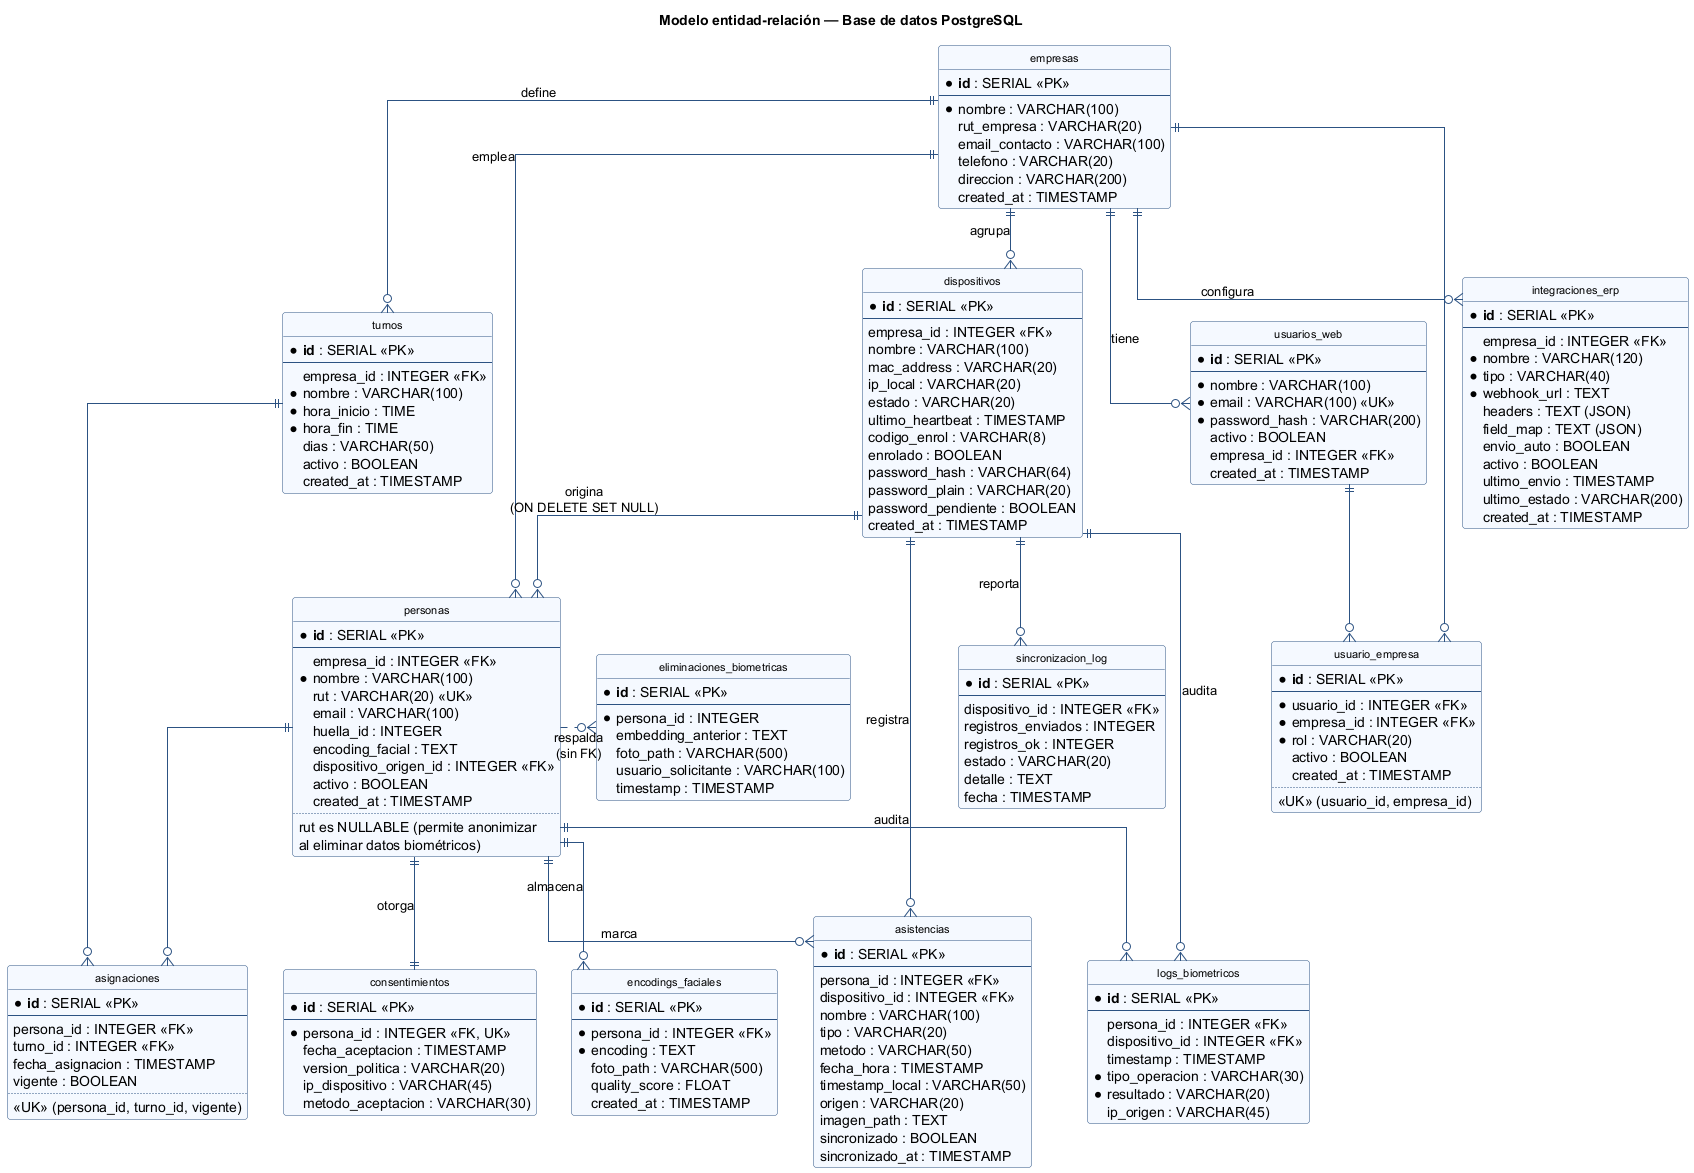
\includegraphics[width=\linewidth]{diagrams/diagrama_er_base_datos.png}
    \caption{Diagrama entidad-relación de la base de datos (14 tablas).}
    \label{fig:db-er}
\end{figure}

Las imágenes faciales, tanto las de registro como las de identificación durante la marcación, viajan del ESP32-CAM al backend por HTTP, como un JPEG crudo en formato application/octet-stream dirigido al endpoint correspondiente (POST /api/facial/registrar o POST /api/facial/identificar). El backend responde en la misma petición indicando si la foto fue aceptada, de modo que el dispositivo no necesita esperar un mensaje aparte para saber el resultado.

MQTT queda reservado para los eventos de estado del dispositivo, que son livianos y no requieren transportar una imagen. Se definen los tópicos esp32/heartbeat/<MAC> para monitorizar la actividad de los dispositivos y esp32/lwt/<MAC> para detectar desconexiones mediante el mecanismo de Last Will Testament (LWT). Para la detección activa de desconexión, se implementó el tópico esp32/ping/<MAC>: el backend publica un ping cada 30 segundos; si el ESP32-CAM no responde con un heartbeat dentro de 60 segundos, se marca como inactivo. La Figura~\ref{fig:flujo_mqtt} resume la topología de publicación y suscripción.

\begin{figure}[H]
  \centering
  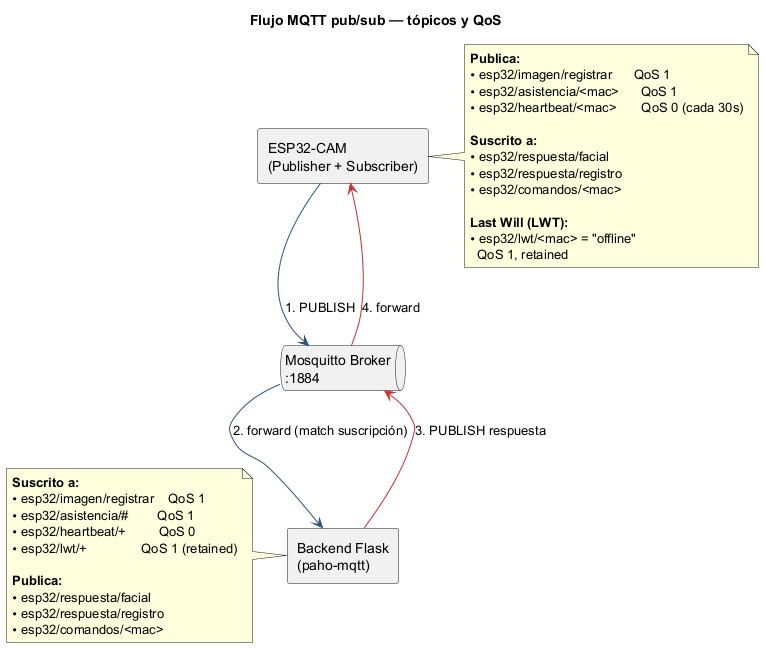
\includegraphics[width=\linewidth]{diagrams/flujo_mqtt_pub_sub.png}
  \caption{Flujo MQTT pub/sub: tópicos, direcciones y QoS entre el ESP32-CAM, el broker Mosquitto y el backend.}
  \label{fig:flujo_mqtt}
\end{figure}

\subsubsection{Implementación}

La implementación de la Iteración 3 se centró en habilitar la comunicación entre el dispositivo ESP32-CAM y el backend desarrollado en Python con Flask \cite{flask_docs}, así como en construir la base de datos PostgreSQL, accedida mediante el adaptador psycopg2 \cite{psycopg2_docs}, que soporta todo el sistema.

\paragraph{Inicialización de la base de datos}

Se implementó el módulo database.py con una función init\_db() que crea todas las tablas del sistema utilizando sentencias CREATE TABLE IF NOT EXISTS, asegurando idempotencia en los despliegues. Adicionalmente, se aplican sentencias ALTER TABLE ADD COLUMN IF NOT EXISTS para garantizar migraciones no destructivas. La función incluye la creación de índices sobre columnas frecuentemente consultadas (persona\_id, dispositivo\_id, fecha\_hora, empresa\_id) y la inserción de datos semilla (empresa por defecto, usuario administrador con contraseña hasheada).

\paragraph{Conexión Wi-Fi del ESP32-CAM y gestión de conectividad}

Para permitir la operación en red, el dispositivo implementa un mecanismo de conexión automática a Wi-Fi mediante la función tryConnectWiFi(). Esta función lee las credenciales desde wifi.json, configura el modo STA y deshabilita el ahorro de energía Wi-Fi (WIFI\_PS\_NONE) para mantener una conexión estable. La verificación continua de conectividad se realiza en verificarConexionWiFi(), que implementa un mecanismo de reintentos con backoff progresivo: tras detectar una desconexión, espera un tiempo creciente antes de reintentar (3s, 6s, 9s, 12s, 15s). Si tras 5 intentos fallidos no se logra reconectar, el dispositivo activa el Access Point como fallback.

El evento ARDUINO\_EVENT\_WIFI\_STA\_DISCONNECTED queda registrado con su código de razón y un contador de desconexiones, información expuesta a través del endpoint /wifi-diag para diagnóstico remoto.

\paragraph{Envío de imágenes faciales por HTTP: registro e identificación}

Tanto el registro como la identificación facial envían la imagen al backend de la misma manera: como JPEG crudo, sin codificarla en Base64, lo que evita el costo de procesamiento y el aumento de tamaño que implica esa codificación. Durante el registro, cuando el usuario presiona el botón de captura en la interfaz del dispositivo, el firmware toma la foto con la cámara en su calidad más alta y la sube de inmediato al backend mediante una petición POST, identificando a la persona con su RUT en una cabecera de la solicitud. El backend procesa la imagen y responde en esa misma petición si quedó aceptada o si hay que repetir la captura, lo que el dispositivo refleja en el contador de fotos de la pantalla de registro.

Durante la identificación (la consulta que ocurre al momento de marcar asistencia), el flujo es prácticamente el mismo a nivel de transporte: la imagen se captura y se envía por HTTP al endpoint de identificación, y el backend responde de forma síncrona indicando a qué persona corresponde el rostro, o un error si no encuentra coincidencia. Usar el mismo mecanismo síncrono para ambos casos simplificó el firmware, que ya no necesita dos rutas distintas para llegar al backend según el tipo de operación.

La Figura~\ref{fig:maquina_estados_esp32} ilustra la máquina de estados completa del proceso de enrolamiento biométrico en el ESP32-CAM, integrando la captura de huella digital (introducida en la Iteración 2) con el envío de la foto de referencia al backend por HTTP descrito en esta sección.

\begin{figure}[H]
  \centering
  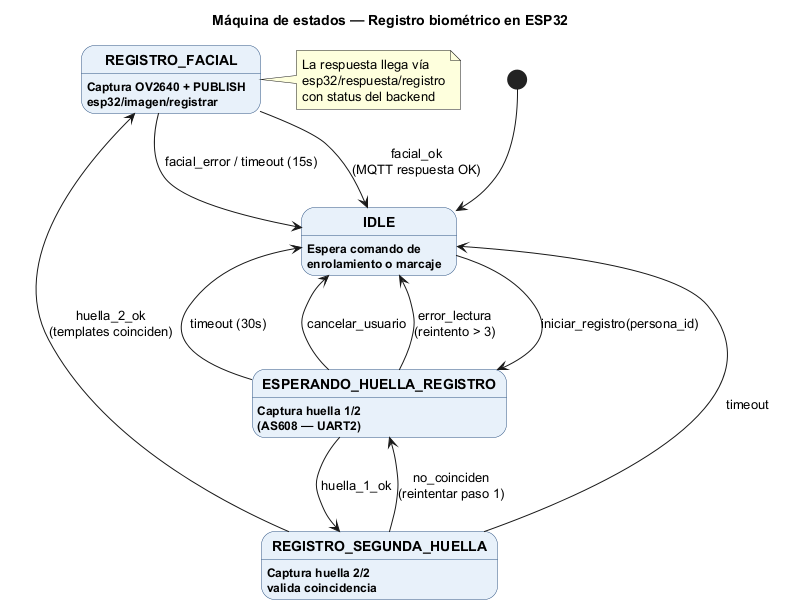
\includegraphics[width=\linewidth]{diagrams/maquina_estados_esp32.png}
  \caption{Máquina de estados del registro biométrico en el ESP32-CAM.}
  \label{fig:maquina_estados_esp32}
\end{figure}

\paragraph{Recepción de imágenes en el backend}

El backend recibe las fotos de registro e identificación a través de los endpoints REST del módulo routes/facial.py, descritos en el diseño de esta sección (ver Anexo B para el detalle completo de endpoints REST y tópicos MQTT). Al llegar una foto de registro, el backend verifica que exista consentimiento biométrico para esa persona, guarda la imagen, extrae el embedding facial y lo cifra antes de almacenarlo; si algo falla en el camino (consentimiento faltante, imagen borrosa, rostro duplicado), responde con el error correspondiente en lugar de dejar la solicitud sin respuesta.

Aparte de las imágenes, el backend mantiene un cliente MQTT para los eventos de estado del dispositivo: procesa los heartbeats, actualizando la IP y la actividad del dispositivo en la base de datos, y los mensajes de desconexión abrupta (LWT), marcándolo como inactivo. También corre en segundo plano una tarea que envía un ping cada 30 segundos a cada dispositivo enrolado, como verificación activa de que sigue en línea. Cada cambio de estado se transmite a los clientes web en tiempo real mediante streaming SSE, para que el panel se actualice sin que el administrador tenga que recargar la página.

\paragraph{Mantenimiento de la conexión MQTT en el ESP32-CAM}

El dispositivo mantiene, en paralelo a sus conexiones HTTP, un cliente MQTT que se conecta al broker si hay uno configurado y el dispositivo tiene red. Soporta URLs con esquema mqtt://, ws:// o wss:// (WebSockets seguros con TLS). Al conectarse, registra un mensaje de último aviso (LWT) para que el backend se entere si el dispositivo se cae de forma abrupta, y queda suscrito al tópico de ping para responder de inmediato cuando el backend pregunta si sigue activo. Este canal MQTT se usa únicamente para esta señalización de estado: ni el registro ni la identificación facial dependen de él.

\paragraph{Envío de datos mediante HTTP desde el ESP32-CAM}

Se implementó la capacidad del ESP32-CAM para comunicarse con la API REST del backend mediante solicitudes HTTP usando la librería HTTPClient. La función auxiliar beginHttp() configura cada petición con timeout de 10 segundos y el header X-Device-MAC para que el backend pueda identificar al dispositivo emisor. Esta función es utilizada por todos los handlers que requieren comunicación con el backend:

\begin{itemize}
    \item sincronizarPersonasDesdeBackend(): Descarga la lista completa de personas desde GET /api/personas y la persiste en personas.json.
    \item sincronizarTurnosDesdeBackend(): Descarga turnos desde GET /api/turnos.
    \item sincronizarAsignacionesDesdeBackend(): Descarga asignaciones desde GET /api/asignaciones.
    \item crearTurnoEnBackend(): Crea un turno en el backend vía POST /api/turnos.
    \item postAsistenciaEnBackend(): Envía una asistencia individual vía POST /api/asistencias.
    \item sincronizarAsistencias(): Envía un lote de asistencias pendientes vía POST /api/asistencias/sync.
\end{itemize}

\paragraph{Implementación de la API REST del backend}

El backend se implementó con Flask, organizando las rutas en blueprints independientes por dominio:
\begin{itemize}
    \item personas\_bp (routes/personas.py): CRUD de personas con validación de email, unicidad de RUT y manejo de empresa.
    \item turnos\_bp (routes/turnos.py): CRUD de turnos con filtro por empresa.
    \item asignaciones\_bp (routes/asignaciones.py): CRUD de asignaciones con verificación de pertenencia a empresa.
    \item asistencias\_bp (routes/asistencias.py): Registro de asistencias individuales y sincronización por lotes.
    \item facial\_bp (routes/facial.py): Endpoints de reconocimiento facial (registro, verificación, identificación 1:N).
    \item dispositivos\_bp (routes/dispositivos.py): Gestión y verificación de dispositivos.
    \item logs\_bp (routes/logs.py): Consulta de logs de sincronización.
    \item erp\_bp (routes/erp.py): CRUD de integraciones ERP y envío de datos.
    \item auth\_bp (routes/auth.py): Autenticación de usuarios del panel web.
\end{itemize}

Cada blueprint se registra en la aplicación Flask principal (app.py), junto con la configuración de CORS para permitir peticiones desde cualquier origen. El backend se ejecuta en el puerto 5000 con modo debug activado y recarga automática deshabilitada para evitar conflictos con el cliente MQTT.

\paragraph{Infraestructura con Docker Compose}

Para garantizar un entorno reproducible, se definió un archivo docker-compose.yml que levanta el broker Mosquitto (imagen eclipse-mosquitto:latest) con el puerto 1884 (externo, mapeado al 1883 interno) para MQTT nativo y el puerto 9001 para WebSockets expuestos, volúmenes para configuración, datos y logs persistentes, y una red bridge dedicada. El backend Flask y la base de datos PostgreSQL pueden ejecutarse en el host o en contenedores adicionales según la configuración de despliegue. La Figura~\ref{fig:docker_despliegue} presenta el diagrama de despliegue completo.

\begin{figure}[H]
  \centering
  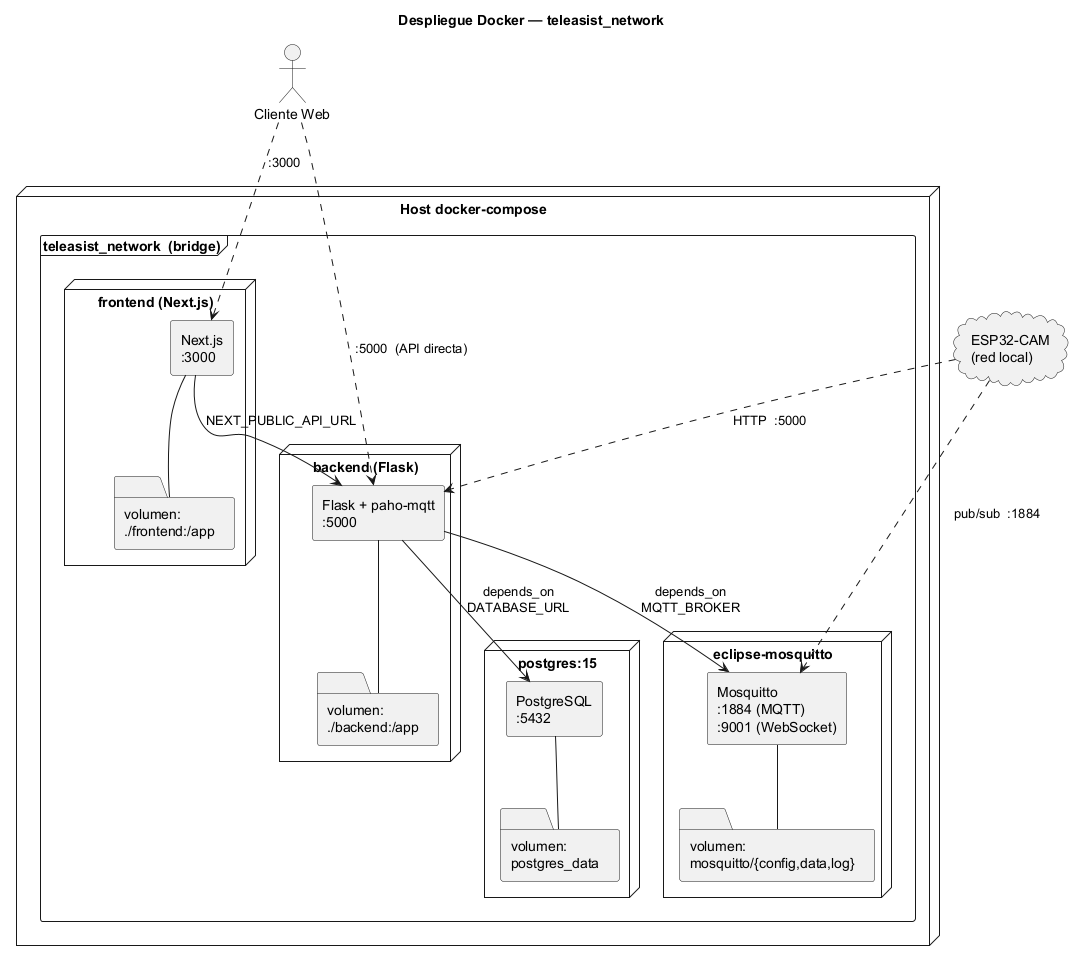
\includegraphics[width=\linewidth]{diagrams/arquitectura_despliegue_docker.png}
  \caption{Arquitectura de despliegue Docker: servicios, puertos, volúmenes y dependencias en la red.}
  \label{fig:docker_despliegue}
\end{figure}

\subsubsection{Pruebas}

Se diseñaron las siguientes pruebas para validar la comunicación y el backend:

\begin{itemize}
    \item \textbf{Prueba de conexión Wi-Fi y reconexión}: Configurar credenciales válidas en el ESP32-CAM, verificar que se conecte correctamente y obtenga una IP. Luego, apagar el router, verificar que el dispositivo detecte la desconexión mediante el evento de sistema y active el mecanismo de reintentos. Finalmente, encender el router y verificar que el dispositivo reconecte automáticamente en menos de 30 segundos.

    \item \textbf{Prueba de envío de imagen facial por HTTP}: Capturar una imagen desde el ESP32-CAM y enviarla al endpoint de registro mediante POST. Verificar que el backend reciba la imagen, la guarde en disco y responda en la misma petición indicando si la foto fue aceptada.

    \item \textbf{Prueba de heartbeat y LWT}: Verificar que, estando el ESP32-CAM conectado, el backend reciba heartbeats periódicos (cada 30 segundos) y actualice el campo ultimo\_heartbeat en la tabla dispositivos. Desconectar el dispositivo abruptamente y verificar que el mensaje LWT se publique y el backend marque el dispositivo como inactivo en menos de 10 segundos.

    \item \textbf{Prueba de ping/pong activo}: Conectar el ESP32-CAM al broker MQTT. Verificar que el backend publique esp32/ping/<MAC> periódicamente (cada 30 segundos) y que el ESP32-CAM responda con un heartbeat que contenga el campo "pong": true. Detener la conectividad del ESP32-CAM y verificar que, tras 60 segundos sin respuesta, el backend marque el dispositivo como inactivo.

    \item \textbf{Prueba de recepción de datos en backend vía HTTP}: Enviar solicitudes POST a /api/personas, /api/turnos, /api/asignaciones y /api/asistencias desde el ESP32-CAM. Verificar que cada solicitud sea procesada correctamente por el backend (código HTTP 200/201) y que los datos queden persistidos en PostgreSQL.

    \item \textbf{Prueba de sincronización por lotes}: Generar 5 marcaciones offline en el ESP32-CAM, conectar el dispositivo a la red y ejecutar la sincronización. Verificar que los 5 registros lleguen al backend vía POST /api/asistencias/sync, que se inserten correctamente y que el dispositivo marque cada registro como sincronizado = true.

    \item \textbf{Prueba de inicialización de base de datos}: Ejecutar init\_db() sobre una base de datos vacía. Verificar que se creen las 14 tablas, los índices y los datos semilla (empresa por defecto y usuario administrador) sin errores.

    \item \textbf{Prueba de latencia de transmisión}: Medir el tiempo total desde que el ESP32-CAM envía una imagen por HTTP hasta que recibe la respuesta de confirmación del backend. Se espera un tiempo menor a 5 segundos en condiciones de red local.
\end{itemize}

\paragraph{Nuevos tópicos MQTT para control y notificación}

En iteraciones posteriores se agregaron los siguientes tópicos al ecosistema MQTT:

\begin{itemize}
    \item backend/comando/<MAC>: Permite al backend enviar comandos remotos al ESP32-CAM. La función enviar\_comando\_dispositivo() en mqtt\_handler.py publica un JSON con el campo comando en este tópico.

    \item backend/notificacion/<MAC>: Utilizado por el módulo eventos\_mqtt.py para notificar a los dispositivos que deben sincronizar sus datos. Cada vez que se crea, actualiza o elimina una persona, turno o asignación, la función notificar\_sincronizacion() publica un mensaje indicando el tipo de entidad y la acción realizada.

    \item esp32/huella/resultado/<huella\_id>: Tópico en el que el ESP32-CAM publica el resultado del enrolamiento de una huella. El backend se suscribe a esp32/huella/resultado/\# y procesa la respuesta, actualizando la persona correspondiente y notificando a través de SSE.
\end{itemize}

\paragraph{Módulo eventos\_mqtt.py}

Se implementó el módulo eventos\_mqtt.py con la función notificar\_sincronizacion(empresa\_id, tipo, accion, registro\_id). Esta función consulta los dispositivos enrolados de la empresa y publica un mensaje en backend/notificacion/<MAC> por cada uno, permitiendo que los ESP32-CAM reciban notificaciones en tiempo real sobre cambios en personas, turnos y asignaciones. Es invocada desde routes/personas.py, routes/turnos.py y routes/asignaciones.py tras cada operación de creación, actualización o eliminación.

\paragraph{Streaming SSE de huellas}

Para mantener actualizados los clientes web durante el enrolamiento de huellas, se implementó el endpoint GET /sse/huellas en app.py. La función broadcast\_huella\_update() difunde los resultados del enrolamiento (recibidos por MQTT en esp32/huella/resultado/\#) a todos los clientes conectados al SSE, permitiendo que el panel web muestre en tiempo real el progreso del registro biométrico.

\subsubsection{Refinamientos posteriores}

\begin{itemize}
    \item \textbf{Decorador @requiere\_dispositivo\_enrolado}: definido en routes/auth.py, valida que el dispositivo asociado a la petición (request.dispositivo\_id) exista en la tabla dispositivos con enrolado = TRUE, devolviendo 403 en caso contrario. Se aplica sobre endpoints biométricos sensibles como /api/facial/registrar, evitando que un dispositivo no autorizado opere sobre datos biométricos.

    \item \textbf{Integridad referencial con ON DELETE SET NULL y RUT nullable}: la columna dispositivo\_origen\_id de la tabla personas (y dispositivo\_id de asistencias) se definió con REFERENCES dispositivos(id) ON DELETE SET NULL, de modo que eliminar un dispositivo no elimina en cascada las personas ni asistencias asociadas, sino que conserva el historial con la referencia en NULL. De forma análoga, la columna rut de personas se migró a nullable (ALTER TABLE personas ALTER COLUMN rut DROP NOT NULL) para permitir el borrado de datos sensibles de una persona sin perder su historial de asistencias.
\end{itemize}


%% ============================================================
%% ITERACIÓN 4: Reconocimiento facial, anti-spoofing y cifrado
%% ============================================================

\subsection{Iteración 4: Reconocimiento facial, anti-spoofing y cifrado biométrico}

Esta iteración incorpora el procesamiento biométrico en el backend: reconocimiento facial con DeepFace, validación anti-spoofing y cifrado de embeddings faciales. El sistema pasa de solo transmitir imágenes a realizar verificación e identificación biométrica.

\subsubsection{Análisis}

Para incorporar el reconocimiento facial al sistema, se evaluaron diversas librerías y modelos de deep learning. Se seleccionó DeepFace por las siguientes razones:

\begin{itemize}
    \item Soporta múltiples modelos de reconocimiento facial (Facenet, VGG-Face, ArcFace, etc.) y detectores (RetinaFace, MTCNN, OpenCV, etc.).
    \item Incluye funcionalidad de anti-spoofing integrada, capaz de distinguir entre un rostro real y una fotografía o pantalla, analizando textura, profundidad y reflectancia de la piel.
    \item Su API en Python es sencilla de integrar con Flask y compatible con las imágenes JPEG capturadas por la cámara OV2640 del ESP32-CAM.
    \item Facenet genera embeddings de 128 dimensiones, optimizando el almacenamiento y la velocidad de comparación.
\end{itemize}

Se identificaron los siguientes requisitos funcionales para esta iteración:

\begin{itemize}
    \item \textbf{Registro facial}: Recibir una imagen del ESP32-CAM, extraer el embedding facial, validar que el rostro no esté duplicado en la base de datos (detección de identidades repetidas) y almacenar el embedding cifrado.
    \item \textbf{Identificación 1:N}: Dada una imagen capturada en vivo, comparar su embedding contra todos los embeddings almacenados y retornar la identidad con mayor coincidencia, si supera el umbral de similitud.
    \item \textbf{Verificación 1:1}: Dada una imagen y un rut, verificar si la imagen corresponde a la persona declarada.
    \item \textbf{Anti-spoofing}: Detectar intentos de suplantación mediante fotografías impresas, pantallas de dispositivos o máscaras, rechazando la captura si no se detecta un rostro real.
    \item \textbf{Cifrado de embeddings}: Los vectores de características faciales (embeddings) son datos biométricos sensibles. Para protegerlos, se deben cifrar antes de persistirlos en la base de datos, utilizando una clave derivada de una variable de entorno.
    \item \textbf{Consentimiento biométrico}: Todo registro facial debe estar precedido por la aceptación explícita de una política de privacidad por parte del trabajador, en cumplimiento de la normativa de protección de datos.
\end{itemize}

\subsubsection{Diseño}

El flujo de procesamiento facial se divide en tres operaciones principales:

\begin{enumerate}
    \item \textbf{Registro} (POST /api/facial/registrar):
    \begin{itemize}
        \item Recibe la imagen como JPEG crudo (application/octet-stream) con el RUT en un header HTTP, que es como la envía el dispositivo, o como JSON con la imagen en Base64, opción que se mantiene para clientes web.
        \item Verifica que exista consentimiento biométrico en la tabla consentimientos. Si no existe, rechaza con HTTP 403.
        \item Guarda la imagen como static/previews/<id>.jpg.
        \item Aplica un \textbf{filtro de calidad de imagen} que mide la nitidez mediante la varianza del Laplaciano \cite{pech2000_laplacian}. Si la imagen es demasiado plana o borrosa (por debajo de un umbral configurable, 50 por defecto), se rechaza como posible intento de suplantación (foto de pantalla o papel) antes de llegar a DeepFace, ahorrando procesamiento innecesario del modelo.
        \item Extrae el embedding con DeepFace usando el modelo Facenet y un detector configurable mediante variable de entorno (FACIAL\_DETECTOR), utilizando MTCNN por defecto por su velocidad (tres veces más rápido que RetinaFace con precisión comparable) y sin anti-spoofing en esta etapa.
        \item Cifra el embedding con Fernet y lo almacena en la tabla encodings\_faciales, que permite acumular múltiples fotos de referencia por persona con distintos ángulos e iluminación, mejorando la precisión en subsecuentes identificaciones.
    \end{itemize}

    El flujo completo de enrolamiento biométrico, desde la creación de la persona en el panel web por parte del administrador, pasando por el registro de huella en dos pasos en el ESP32-CAM, hasta la captura facial enviada por HTTP al backend donde se extrae, cifra y almacena el embedding, se ilustra en el diagrama de secuencia de la Figura~\ref{fig:flujo_enrolamiento} del Anexo C.

    \item \textbf{Identificación 1:N} (POST /api/facial/identificar):
    \begin{itemize}
        \item Recibe la imagen como JPEG crudo (application/octet-stream) desde el ESP32-CAM, o como JSON con Base64 desde la web.
        \item Aplica el mismo filtro de calidad Laplacian como barrera anti-spoofing previa, rechazando imágenes de baja nitidez antes de invocar DeepFace.
        \item Extrae el embedding con DeepFace (anti-spoofing activado mediante anti\_spoofing=True).
        \item Consulta una caché en memoria de embeddings (con TTL configurable, 60 segundos por defecto). Si la caché expiró, recarga todos los embeddings desde la base de datos. Para cada persona, compara contra todos los embeddings almacenados en encodings\_faciales (multi-encoding) y selecciona la menor distancia. Esto mejora la precisión porque el sistema puede reconocer a un trabajador aunque la captura en vivo tenga una iluminación o ángulo diferentes a los de su foto de registro.
        \item Si la menor distancia es inferior al umbral (10.0 para Facenet), retorna el rut correspondiente. En caso contrario, retorna HTTP 404.
    \end{itemize}

    El ciclo de marcaje automático por centinela facial, en el que cada 6 segundos el ESP32-CAM evalúa el sensor PIR, captura una imagen, la envía por HTTP al endpoint de identificación, y según la respuesta del backend registra la asistencia y dispara el push asíncrono a los ERP configurados, se presenta en el diagrama de secuencia de la Figura~\ref{fig:flujo_marcaje} del Anexo C, dado su tamaño.

    \item \textbf{Verificación 1:1} (POST /api/facial/verificar):
    \begin{itemize}
        \item Recibe rut e imagen (Base64).
        \item Descifra todos los embeddings almacenados para esa persona en encodings\_faciales y extrae el embedding de la imagen capturada (con anti-spoofing activado).
        \item Calcula la distancia euclidiana contra cada embedding de referencia y selecciona la menor. Si es menor que 10.0, retorna éxito con el nivel de confianza calculado como max(0, (1 - distancia/20) * 100).
    \end{itemize}
\end{enumerate}

El modelo seleccionado es Facenet por su equilibrio entre precisión y tamaño de embedding (128 dimensiones). El detector facial es configurable mediante variable de entorno (FACIAL\_DETECTOR), utilizando MTCNN por defecto. Si bien RetinaFace ofrece mayor robustez ante variaciones extremas de pose e iluminación, MTCNN es tres veces más rápido y mantiene una precisión comparable para las condiciones típicas de una cámara de control de asistencia (rostro frontal a corta distancia), lo que lo hace más adecuado para un dispositivo embebido como el ESP32-CAM. El umbral de 10.0 para la distancia euclidiana fue elegido con base en la documentación de DeepFace y ajustes empíricos realizados durante el desarrollo.

Para el cifrado de embeddings se utiliza el algoritmo Fernet (AES-128 en modo CBC con HMAC-SHA256 para autenticación), parte de la librería cryptography de Python. La clave de cifrado se deriva aplicando SHA-256 a una variable de entorno (BIOMETRIC\_KEY), garantizando que los embeddings nunca se almacenen en texto plano en la base de datos.

\subsubsection{Implementación}

\paragraph{Procesamiento de imágenes en el backend}

El módulo routes/facial.py implementa los tres endpoints descritos en el diseño. Las funciones auxiliares incluyen:

\begin{itemize}
    \item \_validar\_calidad\_imagen(img\_path): Aplica el filtro Laplaciano (varianza del Laplaciano) sobre la imagen decodificada para medir su nitidez. Si el valor está por debajo del umbral configurable en FACIAL\_NITIDEZ\_UMBRAL (50 por defecto), la imagen se considera borrosa o plana (posible foto de pantalla o papel) y se rechaza antes de llegar a DeepFace, funcionando como una capa adicional de anti-spoofing.
    \item extraer\_embedding(img\_path, anti\_spoofing): Invoca DeepFace.represent() con el modelo Facenet pre-cargado y el detector configurable vía variable de entorno. Si anti\_spoofing=True, activa la detección de suplantación.
    \item guardar\_imagen\_de\_registro(persona\_id, imagen\_b64): Decodifica la imagen Base64, la convierte a RGB con Pillow y la guarda en static/previews/<id>.jpg.
    \item \_verificar\_consentimiento(persona\_id): Consulta la tabla consentimientos para verificar que exista un registro de aceptación.
    \item \_log\_biometrico(persona\_id, dispositivo\_id, tipo\_operacion, resultado): Inserta un registro de auditoría en logs\_biometricos.
\end{itemize}

Además, para optimizar el rendimiento, el modelo Facenet se precarga al iniciar el servidor mediante DeepFace.build\_model('Facenet', task='facial\_recognition'), eliminando la latencia de carga de pesos en la primera solicitud. Los embeddings almacenados en la base de datos se mantienen en una caché en memoria con tiempo de vida configurable (por defecto 60 segundos, mediante FACIAL\_CACHE\_TTL), evitando consultas repetitivas y descifrados a la base de datos en cada identificación. La caché se invalida automáticamente al registrar una nueva foto o al eliminar datos biométricos, garantizando consistencia.

\paragraph{Cifrado y descifrado de embeddings}

El módulo encryption.py proporciona dos funciones:

\begin{itemize}
    \item cifrar\_embedding(embedding): Serializa el embedding como JSON, lo cifra con Fernet y codifica el resultado en Base64 URL-safe.
    \item descifrar\_embedding(cifrado\_str): Decodifica el Base64, descifra con Fernet y deserializa el JSON para obtener el vector original.
\end{itemize}

% =====================================================================
% Diagrama 8 — Pipeline de cifrado biométrico (TikZ)
% Incluir en memoria.tex con:  % =====================================================================
% Diagrama 8 — Pipeline de cifrado biométrico (TikZ)
% Incluir en memoria.tex con:  % =====================================================================
% Diagrama 8 — Pipeline de cifrado biométrico (TikZ)
% Incluir en memoria.tex con:  \input{diagrams/08_pipeline_cifrado_biometrico.tex}
% Requiere en el preámbulo: \usepackage{tikz}
%                           \usetikzlibrary{arrows.meta, positioning, shapes.geometric}
% =====================================================================
\begin{figure}[H]
\centering
\begin{tikzpicture}[
  node distance=1.1cm and 1.3cm,
  every node/.style={font=\small},
  box/.style={draw, rounded corners=3pt, minimum height=1.1cm,
              minimum width=2.7cm, align=center, fill=blue!8,
              drop shadow={opacity=0.15}},
  crypto/.style={draw, rounded corners=3pt, minimum height=1.1cm,
                 minimum width=2.7cm, align=center, fill=orange!20,
                 drop shadow={opacity=0.15}},
  db/.style={draw, cylinder, shape border rotate=90, aspect=0.25,
             minimum height=1.5cm, minimum width=2.5cm,
             align=center, fill=gray!15},
  fallback/.style={draw, dashed, rounded corners=3pt, minimum height=1.0cm,
                   minimum width=2.7cm, align=center, fill=red!8},
  arrow/.style={-{Stealth[length=2.5mm]}, thick},
  darrow/.style={-{Stealth[length=2.5mm]}, thick, dashed, gray!70!black},
  lbl/.style={font=\scriptsize\itshape, text=gray!50!black}
]

% --- Fila superior: cifrado ---
\node[box]                       (emb)    {Embedding\\\scriptsize{\texttt{float[512]}}};
\node[crypto, right=of emb]      (cif)    {\texttt{cifrar\_embedding()}};
\node[crypto, right=of cif]      (fernet) {Fernet\\\scriptsize{AES-128-CBC + HMAC-SHA256}};
\node[db,     right=of fernet]   (dbn)    {PostgreSQL\\\scriptsize{TEXT (base64)}};

% --- Fila inferior: descifrado ---
\node[crypto, below=1.7cm of fernet] (dcif)    {\texttt{descifrar\_embedding()}};
\node[box,    left=of dcif]          (compare) {Comparación\\\scriptsize{DeepFace.verify}};

% --- Fallback ---
\node[fallback, below=0.7cm of dbn] (legacy) {Fallback legacy\\\scriptsize{embedding sin cifrar}};

% --- Flechas principales ---
\draw[arrow] (emb)    -- (cif);
\draw[arrow] (cif)    -- (fernet);
\draw[arrow] (fernet) -- (dbn);
\draw[arrow] (dbn)    |- (dcif);
\draw[arrow] (dcif)   -- (compare);

% --- Camino fallback ---
\draw[darrow] (legacy.west) -| ([xshift=-0.3cm]dcif.south)
              node[pos=0.75, below, font=\scriptsize] {parse directo};

% --- Etiquetas ---
\node[lbl, above=0.1cm of cif] {clave Fernet (\texttt{.env})};
\node[lbl, above=0.1cm of dcif] {misma clave (rotable)};

\end{tikzpicture}
\caption[Pipeline de cifrado biométrico]{Pipeline de cifrado biométrico — Fernet (AES-128-CBC + HMAC-SHA256) con fallback para embeddings legacy almacenados sin cifrar.}
\label{fig:pipeline_cifrado_biometrico}
\end{figure}

% Requiere en el preámbulo: \usepackage{tikz}
%                           \usetikzlibrary{arrows.meta, positioning, shapes.geometric}
% =====================================================================
\begin{figure}[H]
\centering
\begin{tikzpicture}[
  node distance=1.1cm and 1.3cm,
  every node/.style={font=\small},
  box/.style={draw, rounded corners=3pt, minimum height=1.1cm,
              minimum width=2.7cm, align=center, fill=blue!8,
              drop shadow={opacity=0.15}},
  crypto/.style={draw, rounded corners=3pt, minimum height=1.1cm,
                 minimum width=2.7cm, align=center, fill=orange!20,
                 drop shadow={opacity=0.15}},
  db/.style={draw, cylinder, shape border rotate=90, aspect=0.25,
             minimum height=1.5cm, minimum width=2.5cm,
             align=center, fill=gray!15},
  fallback/.style={draw, dashed, rounded corners=3pt, minimum height=1.0cm,
                   minimum width=2.7cm, align=center, fill=red!8},
  arrow/.style={-{Stealth[length=2.5mm]}, thick},
  darrow/.style={-{Stealth[length=2.5mm]}, thick, dashed, gray!70!black},
  lbl/.style={font=\scriptsize\itshape, text=gray!50!black}
]

% --- Fila superior: cifrado ---
\node[box]                       (emb)    {Embedding\\\scriptsize{\texttt{float[512]}}};
\node[crypto, right=of emb]      (cif)    {\texttt{cifrar\_embedding()}};
\node[crypto, right=of cif]      (fernet) {Fernet\\\scriptsize{AES-128-CBC + HMAC-SHA256}};
\node[db,     right=of fernet]   (dbn)    {PostgreSQL\\\scriptsize{TEXT (base64)}};

% --- Fila inferior: descifrado ---
\node[crypto, below=1.7cm of fernet] (dcif)    {\texttt{descifrar\_embedding()}};
\node[box,    left=of dcif]          (compare) {Comparación\\\scriptsize{DeepFace.verify}};

% --- Fallback ---
\node[fallback, below=0.7cm of dbn] (legacy) {Fallback legacy\\\scriptsize{embedding sin cifrar}};

% --- Flechas principales ---
\draw[arrow] (emb)    -- (cif);
\draw[arrow] (cif)    -- (fernet);
\draw[arrow] (fernet) -- (dbn);
\draw[arrow] (dbn)    |- (dcif);
\draw[arrow] (dcif)   -- (compare);

% --- Camino fallback ---
\draw[darrow] (legacy.west) -| ([xshift=-0.3cm]dcif.south)
              node[pos=0.75, below, font=\scriptsize] {parse directo};

% --- Etiquetas ---
\node[lbl, above=0.1cm of cif] {clave Fernet (\texttt{.env})};
\node[lbl, above=0.1cm of dcif] {misma clave (rotable)};

\end{tikzpicture}
\caption[Pipeline de cifrado biométrico]{Pipeline de cifrado biométrico — Fernet (AES-128-CBC + HMAC-SHA256) con fallback para embeddings legacy almacenados sin cifrar.}
\label{fig:pipeline_cifrado_biometrico}
\end{figure}

% Requiere en el preámbulo: \usepackage{tikz}
%                           \usetikzlibrary{arrows.meta, positioning, shapes.geometric}
% =====================================================================
\begin{figure}[H]
\centering
\begin{tikzpicture}[
  node distance=1.1cm and 1.3cm,
  every node/.style={font=\small},
  box/.style={draw, rounded corners=3pt, minimum height=1.1cm,
              minimum width=2.7cm, align=center, fill=blue!8,
              drop shadow={opacity=0.15}},
  crypto/.style={draw, rounded corners=3pt, minimum height=1.1cm,
                 minimum width=2.7cm, align=center, fill=orange!20,
                 drop shadow={opacity=0.15}},
  db/.style={draw, cylinder, shape border rotate=90, aspect=0.25,
             minimum height=1.5cm, minimum width=2.5cm,
             align=center, fill=gray!15},
  fallback/.style={draw, dashed, rounded corners=3pt, minimum height=1.0cm,
                   minimum width=2.7cm, align=center, fill=red!8},
  arrow/.style={-{Stealth[length=2.5mm]}, thick},
  darrow/.style={-{Stealth[length=2.5mm]}, thick, dashed, gray!70!black},
  lbl/.style={font=\scriptsize\itshape, text=gray!50!black}
]

% --- Fila superior: cifrado ---
\node[box]                       (emb)    {Embedding\\\scriptsize{\texttt{float[512]}}};
\node[crypto, right=of emb]      (cif)    {\texttt{cifrar\_embedding()}};
\node[crypto, right=of cif]      (fernet) {Fernet\\\scriptsize{AES-128-CBC + HMAC-SHA256}};
\node[db,     right=of fernet]   (dbn)    {PostgreSQL\\\scriptsize{TEXT (base64)}};

% --- Fila inferior: descifrado ---
\node[crypto, below=1.7cm of fernet] (dcif)    {\texttt{descifrar\_embedding()}};
\node[box,    left=of dcif]          (compare) {Comparación\\\scriptsize{DeepFace.verify}};

% --- Fallback ---
\node[fallback, below=0.7cm of dbn] (legacy) {Fallback legacy\\\scriptsize{embedding sin cifrar}};

% --- Flechas principales ---
\draw[arrow] (emb)    -- (cif);
\draw[arrow] (cif)    -- (fernet);
\draw[arrow] (fernet) -- (dbn);
\draw[arrow] (dbn)    |- (dcif);
\draw[arrow] (dcif)   -- (compare);

% --- Camino fallback ---
\draw[darrow] (legacy.west) -| ([xshift=-0.3cm]dcif.south)
              node[pos=0.75, below, font=\scriptsize] {parse directo};

% --- Etiquetas ---
\node[lbl, above=0.1cm of cif] {clave Fernet (\texttt{.env})};
\node[lbl, above=0.1cm of dcif] {misma clave (rotable)};

\end{tikzpicture}
\caption[Pipeline de cifrado biométrico]{Pipeline de cifrado biométrico — Fernet (AES-128-CBC + HMAC-SHA256) con fallback para embeddings legacy almacenados sin cifrar.}
\label{fig:pipeline_cifrado_biometrico}
\end{figure}


\paragraph{Actualización y eliminación de datos faciales}

Se implementó el endpoint PUT /api/facial/actualizar/<persona\_id> que permite reemplazar el embedding y la foto de una persona existente. También se implementó DELETE /api/personas/<id>/datos-biometricos que elimina el embedding facial, la huella asociada, la foto en disco y el consentimiento, pero conserva los registros de asistencia históricos. La eliminación queda registrada en la tabla eliminaciones\_biometricas para trazabilidad.

Se implementó además el endpoint POST /api/facial/agregar-foto que permite agregar fotos de referencia adicionales a una persona ya registrada, sin reemplazar las existentes. Cada nueva foto pasa por el mismo filtro de calidad Laplacian y se almacena como un nuevo registro en encodings\_faciales. Esta funcionalidad de enrolamiento progresivo permite mejorar la precisión del sistema a lo largo del tiempo: si un trabajador experimenta falsos rechazos, se le pueden agregar más fotos de referencia con distintos ángulos o condiciones de iluminación, aumentando la robustez del reconocimiento sin necesidad de rehacer el registro completo.

\subsubsection{Pruebas}

Se diseñaron las siguientes pruebas para validar el módulo de reconocimiento facial:

\begin{itemize}
    \item \textbf{Prueba de registro facial exitoso}: Enviar una imagen facial válida junto con un rut que tenga consentimiento registrado. Verificar que el backend extraiga el embedding, lo almacene cifrado y responda con HTTP 200.

    \item \textbf{Prueba de detección de duplicados}: Registrar una segunda imagen del mismo rostro para otra persona. Verificar que el backend detecte la similitud (distancia < 10.0) y rechace el registro con HTTP 409, indicando el nombre de la persona con la que coincide.

    \item \textbf{Prueba de rechazo por falta de consentimiento}: Intentar registrar un rostro para una persona sin consentimiento biométrico. Verificar que el backend rechace la operación con HTTP 403.

    \item \textbf{Prueba de identificación 1:N}: Registrar 3 personas con sus respectivas fotos. Enviar una nueva foto de una de ellas al endpoint de identificación. Verificar que el backend retorne el rut correcto.

    \item \textbf{Prueba de identificación con rostro desconocido}: Enviar una foto de una persona no registrada. Verificar que el backend retorne HTTP 404 y registre el intento fallido en logs\_biometricos.

    \item \textbf{Prueba de anti-spoofing con fotografía impresa}: Capturar una foto de un rostro registrado desde una pantalla o impresión y enviarla al endpoint de identificación. Verificar que DeepFace con anti\_spoofing=True rechace la imagen por no detectar un rostro real (excepción ValueError con mensaje ``Spoof detected'').

    \item \textbf{Prueba de resistencia a condiciones de iluminación}: Capturar imágenes del mismo rostro bajo 3 condiciones de iluminación (luz natural, luz artificial tenue, contraluz). Verificar que los 3 embeddings generados mantengan distancia euclidiana entre sí menor a 10.0 y que el sistema identifique correctamente a la persona.

    \item \textbf{Prueba de cifrado y descifrado}: Almacenar un embedding en la base de datos y verificar que el valor en la columna encoding\_facial no sea legible (no contenga los números del vector en texto plano). Luego, recuperar el registro y descifrar el embedding; verificar que el vector original se reconstruya idénticamente.

    \item \textbf{Prueba de eliminación de datos biométricos}: Ejecutar el endpoint de eliminación de datos biométricos para una persona con rostro registrado. Verificar que el embedding se elimine de la base de datos, que la foto se borre del disco, que el consentimiento se elimine, que los registros de asistencia se conserven y que quede una entrada en eliminaciones\_biometricas.

    \item \textbf{Prueba de filtro de calidad de imagen}: Enviar al endpoint de registro una imagen deliberadamente borrosa o una foto de una pantalla (baja varianza de Laplacian). Verificar que el backend rechace la imagen antes de invocar DeepFace, retornando un error de calidad insuficiente.

    \item \textbf{Prueba de múltiples fotos de referencia}: Registrar una persona con una foto frontal. Luego, agregar una segunda foto de la misma persona con distinto ángulo mediante POST /api/facial/agregar-foto. Realizar una identificación con una tercera foto y verificar que el sistema reconozca a la persona correctamente, comparando contra ambos embeddings de referencia.
    
    \item \textbf{Prueba de caché de embeddings}: Realizar una identificación exitosa y verificar los tiempos de respuesta. Realizar una segunda identificación inmediatamente después; verificar que el tiempo sea significativamente menor porque los embeddings se sirvieron desde la caché en memoria sin consultar la base de datos.
\end{itemize}

\paragraph{Endpoint identificar-o-registrar}

Se implementó el endpoint POST /api/facial/identificar-o-registrar que combina ambos flujos en una sola llamada: primero intenta identificar a la persona por su rostro; si la identificación es exitosa, retorna los datos de la persona; si falla y se proporciona un RUT con consentimiento biométrico, registra automáticamente la nueva persona con el embedding facial extraído. Este endpoint facilita el enrolamiento progresivo en el dispositivo: un trabajador puede colocarse frente al ESP32-CAM y, si ya está registrado, se marca su asistencia; si no, el sistema lo registra sobre la marcha. El endpoint incluye validación de calidad de imagen, anti-spoofing y log biométrico tanto para identificación como para registro.

\subsubsection{Refinamientos posteriores}

\begin{itemize}
    \item \textbf{Transmisión de imágenes vía octet-stream}: el envío de la imagen facial migró de un esquema basado en JSON con la foto codificada en Base64 a un envío binario directo (Content-Type: application/octet-stream) con el RUT o la MAC del dispositivo en un header HTTP (X-RUT / X-Device-MAC). El backend mantiene compatibilidad retroactiva con el formato Base64 como \textit{fallback}. El cambio elimina el overhead de codificación Base64 (aproximadamente 33\% de tamaño adicional) y simplifica el firmware, que ahora envía directamente el buffer JPEG capturado por la cámara (fb->buf, fb->len).

    \item \textbf{Captura de 3 fotos de referencia por persona}: el flujo de registro se extendió de una sola foto a tres capturas sucesivas (FOTOS\_REQUERIDAS = 3 en el firmware), idealmente frontal y de ambos perfiles, generando tres embeddings independientes almacenados en la tabla encodings\_faciales. Esto mejora la tasa de identificación ante variaciones de ángulo o iluminación, ya que la comparación 1:N evalúa contra todos los embeddings de referencia disponibles.
\end{itemize}


%% ============================================================
%% ITERACIÓN 5: Autenticación, multi-tenant y enrolamiento
%% ============================================================

\subsection{Iteración 5: Autenticación, multi-tenant y enrolamiento de dispositivos}

La quinta iteración incorpora la capa de seguridad y administración del sistema: autenticación de usuarios del panel web mediante JWT, un modelo multi-tenant que permite a múltiples empresas operar sobre la misma instancia del backend con datos aislados, y un mecanismo seguro de enrolamiento de dispositivos ESP32-CAM mediante PIN de un solo uso.

\subsubsection{Análisis}

El sistema, al estar orientado a un entorno empresarial, requiere que diferentes organizaciones puedan utilizar la misma plataforma sin que sus datos se mezclen. Asimismo, el panel web administrativo debe restringir el acceso según el rol del usuario. Finalmente, cada dispositivo ESP32-CAM debe ser vinculado de forma segura a una empresa específica, evitando que dispositivos no autorizados inyecten datos en el sistema.

Los requisitos identificados son:

\begin{itemize}
    \item \textbf{Multi-tenant}: Cada entidad (persona, turno, asignación, asistencia, dispositivo) debe pertenecer a una empresa. Las consultas deben filtrarse por empresa según el contexto del usuario autenticado. El administrador global (rol admin) tiene visibilidad sobre todas las empresas.
    \item \textbf{Autenticación JWT}: El panel web backend debe requerir autenticación para operaciones sensibles. Los tokens JWT (JSON Web Tokens), firmados con HMAC-SHA256, transportan el ID de usuario, la empresa seleccionada y su rol. Tienen expiración de 24 horas.
    \item \textbf{Roles de usuario}: Se definen tres roles jerárquicos:
    \begin{itemize}
        \item admin: Acceso total al sistema, puede crear empresas, gestionar todos los usuarios y dispositivos.
        \item empleador: Acceso limitado a los datos de su empresa; puede gestionar trabajadores, turnos y ver asistencias.
        \item trabajador: Acceso restringido a sus propios datos de asistencia.
    \end{itemize}
    \item \textbf{Enrolamiento de dispositivos}: Un administrador genera un PIN de 8 caracteres en el panel web. Ese PIN se ingresa en el ESP32-CAM (vía web embebida), que lo envía al backend junto con su MAC address. Si el PIN es válido y no ha sido usado, el dispositivo queda enrolado y asociado a la empresa correspondiente.
    \item \textbf{Auto-registro de empresas}: Se requiere un endpoint público que permita a una nueva organización registrarse de forma autónoma en el sistema, sin intervención del administrador central. La empresa proporciona sus datos (nombre, RUT, email, etc.) y los datos del usuario administrador; el sistema crea la empresa, el usuario, y la asociación entre ambos con rol admin en una sola transacción atómica, retornando un token JWT para que el nuevo administrador quede autenticado inmediatamente. Esto facilita el despliegue del sistema en nuevos clientes sin requerir configuración manual previa.
    \item \textbf{Monitorización de dispositivos}: Una vez enrolado, el ESP32-CAM envía heartbeats periódicos vía MQTT. El backend actualiza el estado del dispositivo (activo) y registra su última actividad. Un proceso watchdog marca como inactivo a los dispositivos que no han enviado heartbeat en más de 90 segundos.
\end{itemize}

\subsubsection{Diseño}

\paragraph{Modelo de datos multi-tenant}

La estrategia multi-tenant se implementa a nivel de base de datos mediante una columna empresa\_id en las tablas personas, turnos, dispositivos, integraciones\_erp y asistencias (esta última a través de la relación con personas). La tabla empresas actúa como entidad raíz del tenant. La tabla asociativa usuario\_empresa vincula usuarios con empresas y define el rol que cada usuario tiene en cada empresa, permitiendo que un mismo usuario tenga roles distintos en diferentes organizaciones.

\paragraph{Flujo de autenticación}

\begin{enumerate}
    \item El usuario envía email y contraseña al endpoint POST /api/auth/login.
    \item El backend valida las credenciales contra la tabla usuarios\_web usando bcrypt.
    \item Se consultan las empresas asociadas al usuario en usuario\_empresa.
    \item Si el usuario pertenece a una sola empresa, se selecciona automáticamente. Si pertenece a varias, se retorna la lista para que elija.
    \item Se genera un token JWT con payload: user\_id, empresa\_id, rol, persona\_id (si es trabajador) y exp (24 horas).
    \item Las peticiones subsecuentes deben incluir el header Authorization: Bearer <token>.
\end{enumerate}

Se implementan dos niveles de protección para los endpoints:
\begin{itemize}
    \item @token\_required: Exige token JWT válido.
    \item @requiere\_rol('admin', 'empleador'): Además del token, exige que el rol del usuario esté en la lista permitida.
    \item @token\_opcional: Intenta extraer el token si está presente; si no, permite el acceso sin autenticación (útil para endpoints consumidos por el ESP32-CAM, que en su lugar envían el header X-Device-MAC para identificar la empresa).
\end{itemize}

\begin{figure}[H]
  \centering
  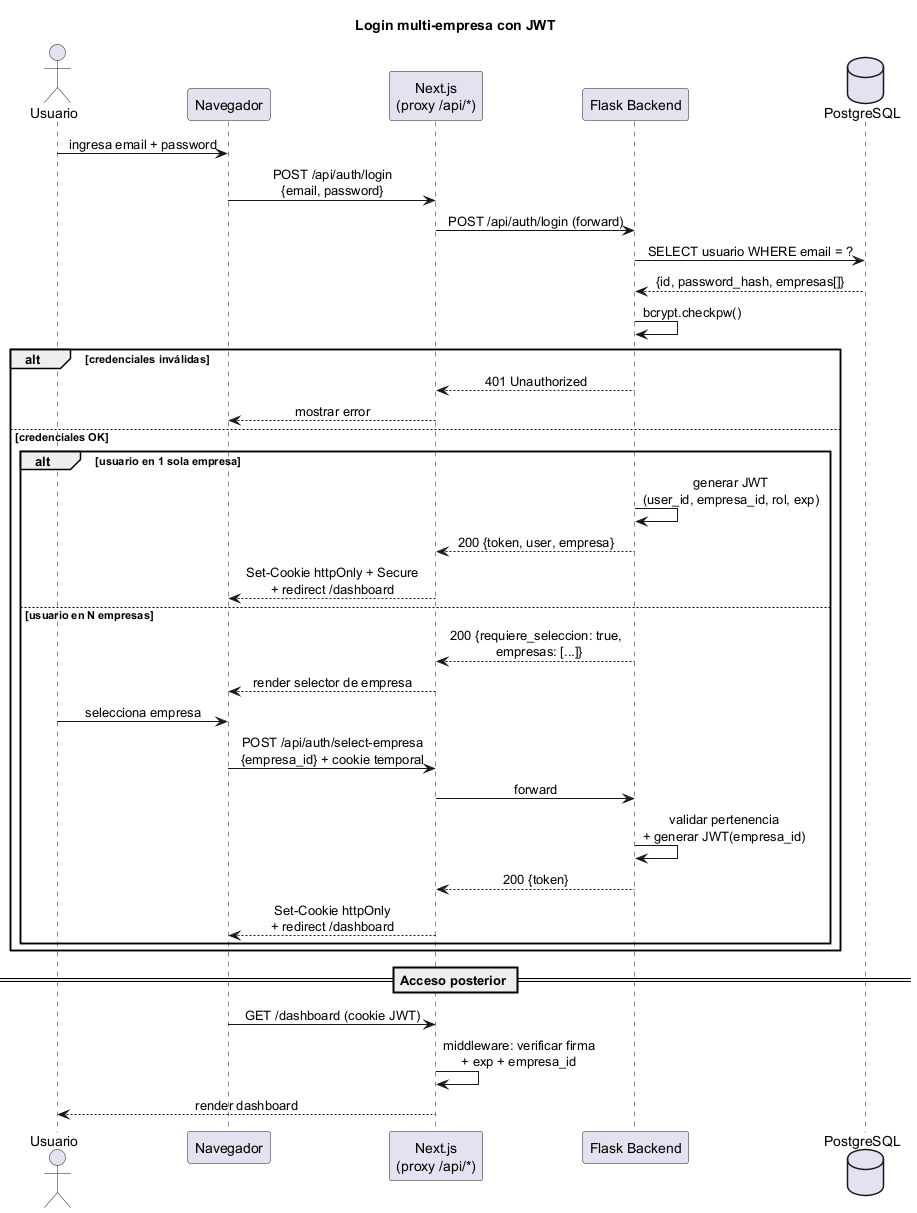
\includegraphics[width=0.95\linewidth]{diagrams/flujo_login_jwt.png}
  \caption{Diagrama de secuencia del login multi-empresa con JWT.}
  \label{fig:flujo_login_jwt}
\end{figure}

\paragraph{Flujo de enrolamiento de dispositivos}

\begin{enumerate}
    \item Un administrador o empleador accede a POST /api/dispositivos/generar-pin desde el panel web, especificando un nombre para el dispositivo. El backend genera un PIN alfanumérico de 8 caracteres (ej. A3B9XK2M) usando secrets.choice() y lo inserta en la tabla dispositivos con enrolado = FALSE.
    \item El administrador ingresa el PIN en la interfaz web del ESP32-CAM (/wifi-setup).
    \item Al guardar la configuración, el ESP32-CAM envía POST /api/dispositivos/enrolar con el PIN, su MAC address y su IP local.
    \item El backend valida el PIN, asocia la MAC y la IP al dispositivo, marca enrolado = TRUE y limpia el PIN para que no pueda ser reutilizado.
    \item A partir de este momento, el ESP32-CAM envía heartbeats periódicos y el backend lo reconoce como dispositivo autorizado de la empresa.
\end{enumerate}

\paragraph{Heartbeat y Last Will Testament (LWT)}

El ESP32-CAM publica periódicamente (cada 30 segundos) un mensaje JSON en el tópico esp32/heartbeat/<MAC> con su MAC, timestamp e IP. El backend actualiza el campo ultimo\_heartbeat y marca el estado como activo. Al conectarse al broker MQTT, el ESP32-CAM configura un mensaje LWT en el tópico esp32/lwt/<MAC> con \{"estado": "inactivo"\}. Si el dispositivo se desconecta abruptamente, el broker publica automáticamente el LWT, y el backend marca el dispositivo como inactivo.

Además del LWT y el watchdog pasivo, se implementó un ping activo como tercera capa de detección: un hilo device\_pinger() publica periódicamente (cada 30 segundos) un mensaje en el tópico esp32/ping/<MAC>. El ESP32-CAM, al recibirlo, responde inmediatamente publicando un heartbeat con el campo "pong": true. Si el backend no recibe respuesta dentro de 60 segundos, marca el dispositivo como inactivo. Este mecanismo permite detectar desconexiones incluso cuando el mensaje LWT no llega al broker (por ejemplo, por pérdida abrupta de conectividad de red). Adicionalmente, un hilo device\_watchdog ejecutado cada 60 segundos verifica qué dispositivos no han enviado heartbeat en más de 90 segundos y los marca como inactivos, constituyendo una capa de respaldo adicional.

\subsubsection{Implementación}

\paragraph{Módulo de autenticación}

El módulo routes/auth.py implementa:

\begin{itemize}
    \item login(): Valida credenciales con bcrypt, determina la empresa (con selección múltiple si aplica), vincula al trabajador con su persona\_id si el rol es trabajador, y genera el token JWT.
    \item register(): Permite a administradores y empleadores crear nuevos usuarios, asignándoles rol y empresa. Si el email ya existe, se agrega la nueva asociación usuario\_empresa en lugar de duplicar el usuario.
    \item me(): Retorna los datos del usuario autenticado, incluyendo sus empresas y rol actual.
    \item cambiar\_password(): Permite al usuario cambiar su contraseña validando la actual.
    \item generar\_pin\_enrolamiento(): Crea un PIN para enrolar un nuevo dispositivo.
    \item enrolar\_dispositivo(): Valida el PIN y completa el enrolamiento del ESP32-CAM.
    \item listar\_usuarios(), eliminar\_usuario(), listar\_empresas(), crear\_empresa(): Operaciones administrativas con control de roles.
    \item register\_company(): Endpoint público POST /api/auth/register-company que permite el auto-registro de una nueva empresa. Recibe los datos de la organización (nombre, RUT, email, teléfono, dirección) y del usuario administrador (nombre, email, contraseña). En una única transacción atómica crea la empresa, el usuario con hash bcrypt, y la asociación usuario\_empresa con rol admin. Retorna un token JWT para autenticar inmediatamente al nuevo administrador.
\end{itemize}

Los decoradores @token\_required, @token\_opcional y @requiere\_rol se definen en el mismo módulo. El decorador @token\_opcional incluye lógica para inferir la empresa a partir del header X-Device-MAC cuando no hay token JWT presente, buscando la MAC en la tabla de dispositivos. Si la MAC no existe, automáticamente crea un nuevo registro en dispositivos con estado pendiente, lo que permite que los ESP32-CAM comiencen a enviar datos incluso antes de ser formalmente enrolados.

\paragraph{Gestión de dispositivos}

El módulo routes/dispositivos.py implementa:

\begin{itemize}
    \item GET /api/dispositivos: Lista los dispositivos con su estado, MAC, IP y empresa.
    \item PUT /api/dispositivos/<id>: Actualiza el nombre del dispositivo.
    \item DELETE /api/dispositivos/<id>: Elimina un dispositivo (admin) o lo desvincula de la empresa (empleador).
    \item POST /api/dispositivos/verificar: Prueba conectividad con un dispositivo dada su IP, consultando el endpoint /estado del ESP32-CAM.
\end{itemize}

\paragraph{Monitorización vía MQTT}

En el módulo mqtt\_handler.py, la función on\_message maneja los tópicos de heartbeat y LWT:

\begin{itemize}
    \item esp32/heartbeat/<MAC>: Actualiza ultimo\_heartbeat, estado = 'activo' y opcionalmente ip\_local del dispositivo.
    \item esp32/lwt/<MAC>: Marca estado = 'inactivo' en la base de datos.
\end{itemize}

El watchdog (device\_watchdog) ejecuta un barrido inicial al arrancar (todos los dispositivos se marcan inactivos hasta que envíen su primer heartbeat) y luego verifica cada 60 segundos los heartbeats vencidos.

\subsubsection{Pruebas}

Se diseñaron las siguientes pruebas para validar la autenticación, el multi-tenant y el enrolamiento:

\begin{itemize}
    \item \textbf{Prueba de login exitoso}: Enviar credenciales válidas del administrador por defecto (admin@empresa.cl / admin123). Verificar que se reciba un token JWT, los datos del usuario y su empresa. Decodificar el token y verificar que contenga user\_id, empresa\_id y rol = admin.

    \item \textbf{Prueba de login con múltiples empresas}: Crear una segunda empresa y asignar el mismo usuario a ella con rol empleador. Iniciar sesión sin especificar empresa. Verificar que el backend retorne la lista de empresas disponibles. Luego, iniciar sesión especificando una empresa y verificar que el token refleje esa selección.

    \item \textbf{Prueba de rechazo de credenciales inválidas}: Intentar login con contraseña incorrecta. Verificar HTTP 401 y mensaje ``Credenciales inválidas''.

    \item \textbf{Prueba de acceso sin token}: Intentar acceder a GET /api/personas sin enviar header Authorization, desde un cliente sin X-Device-MAC. Verificar que el endpoint responda correctamente (acceso público o con datos limitados según el decorador).

    \item \textbf{Prueba de acceso con rol insuficiente}: Autenticarse como trabajador e intentar crear un turno (POST /api/turnos). Verificar HTTP 403 y mensaje ``Permisos insuficientes''.

    \item \textbf{Prueba de aislamiento multi-tenant}: Crear dos empresas (A y B), registrar una persona en cada una. Autenticarse como empleador de la empresa A y solicitar GET /api/personas. Verificar que solo se retornen las personas de la empresa A.

    \item \textbf{Prueba de generación de PIN}: Autenticarse como empleador y solicitar POST /api/dispositivos/generar-pin. Verificar que se reciba un PIN de 8 caracteres alfanuméricos y que en la base de datos exista un dispositivo con enrolado = FALSE.

    \item \textbf{Prueba de enrolamiento exitoso}: Con un PIN generado, enviar POST /api/dispositivos/enrolar con el PIN, una MAC y una IP. Verificar que el backend marque el dispositivo como enrolado, asocie la MAC y limpie el PIN. Verificar que el mismo PIN no pueda usarse una segunda vez (HTTP 409).

    \item \textbf{Prueba de heartbeat y estado}: Simular heartbeats desde un dispositivo enrolado. Verificar que el estado en la base de datos sea activo. Detener los heartbeats por más de 90 segundos y verificar que el watchdog marque el dispositivo como inactivo.

    \item \textbf{Prueba de LWT}: Conectar el ESP32-CAM al broker MQTT, verificar que el backend reciba el heartbeat y lo marque activo. Desconectar el dispositivo abruptamente (corte de energía). Verificar que el broker publique el LWT y el backend actualice el estado a inactivo en menos de 10 segundos.

    \item \textbf{Prueba de auto-registro de empresa}: Enviar una solicitud a POST /api/auth/register-company con los datos de una nueva empresa y su administrador. Verificar que se cree la empresa en la base de datos, que el usuario administrador se cree con contraseña encriptada (bcrypt), que exista la asociación usuario\_empresa con rol admin, y que el backend retorne un token JWT válido que permita acceder a endpoints protegidos. Verificar que un segundo intento con el mismo email de administrador retorne HTTP 409 (Conflicto).
\end{itemize}

\subsubsection{Refinamientos posteriores}

\begin{itemize}
    \item "\textbf{token\_opcional}": el decorador token\_opcional, que permite que un mismo endpoint acepte tanto usuarios web autenticados por JWT como dispositivos ESP32 identificados por el header X-Device-MAC, inicialmente creaba un registro nuevo en dispositivos si la MAC no existía en la base de datos. Este comportamiento se eliminó: ahora el decorador únicamente busca y vincula dispositivos ya existentes, dejando la creación exclusivamente al flujo explícito de enrolamiento con PIN. El cambio cierra una vía por la que un dispositivo no autorizado podía aparecer en el sistema sin pasar por el control del administrador o empleador.

    \item \textbf{PIN de enrolamiento por empresa}: la generación de PIN (POST /api/auth/dispositivos/generar-pin) quedó condicionada al rol de quien la solicita: un administrador puede generar el PIN para cualquier empresa indicada en la petición, mientras que un empleador solo puede generarlo para la empresa a la que pertenece (request.empresa\_id). El dispositivo creado queda asociado a esa empresa desde el momento de la generación del PIN, reforzando el aislamiento multi-tenant también a nivel de hardware enrolado.
\end{itemize}


%% ============================================================
%% ITERACIÓN 6: Módulo antifraude y validación previa a la captura
%% ============================================================

\subsection{Iteración 6: Módulo antifraude y validación previa a la captura}

Esta iteración implementa la prevención de suplantación de identidad en el ESP32-CAM mediante detección física de presencia, control de iluminación y procesamiento biométrico. Si bien el plan original contemplaba un sensor infrarrojo (IR) dedicado para detectar intentos de suplantación con fotografías, el enfoque implementado evolucionó hacia una solución de múltiples capas que resultó más robusta y prescindió del sensor IR adicional.

\subsubsection{Análisis}

El análisis de escenarios de suplantación identificó los siguientes vectores de ataque potenciales contra el sistema de reconocimiento facial del ESP32-CAM:

\begin{itemize}
    \item \textbf{Fotografía impresa}: Un atacante presenta una foto del rostro de un trabajador legítimo frente a la cámara.
    \item \textbf{Pantalla de dispositivo}: Un atacante muestra un video o imagen del trabajador en la pantalla de un teléfono o tablet.
    \item \textbf{Ausencia de presencia real}: La cámara captura sin que haya una persona físicamente frente al dispositivo (falsos positivos del sensor de movimiento).
\end{itemize}

Inicialmente se planificó el uso de un sensor IR dedicado que permitiera detectar la presencia de un rostro real mediante la emisión y recepción de luz infrarroja, cuya reflectancia difiere entre piel humana y superficies planas como papel o pantallas. Sin embargo, durante el desarrollo se identificaron dos factores que motivaron el cambio de estrategia:

\begin{enumerate}
    \item \textbf{Disponibilidad de GPIO}: El ESP32-CAM tiene una cantidad muy limitada de pines GPIO disponibles tras la asignación del bus paralelo de la cámara. Destinar un pin adicional al sensor IR hubiera requerido sacrificar otra funcionalidad (como el sensor PIR de presencia o el control PWM del flash).

    \item \textbf{Madurez del anti-spoofing por software}: DeepFace, la librería seleccionada para el reconocimiento facial, incorpora un detector de suplantación (\textbf{anti-spoofing}) basado en redes neuronales convolucionales que analiza micro-texturas, reflectancia de la piel y profundidad en la imagen capturada. Este detector es capaz de distinguir entre un rostro real tridimensional y una superficie plana (foto, pantalla) con una precisión comparable o superior a la de sensores IR de bajo costo como los inicialmente considerados.
\end{enumerate}

En consecuencia, se adoptó un enfoque de múltiples capas que combina:

\begin{enumerate}
    \item \textbf{Detección física de presencia (PIR)}: Un sensor infrarrojo pasivo (PIR) que detecta el calor corporal, activando el sistema de captura solo cuando hay una persona real frente al dispositivo. Esto elimina falsos positivos del software y reduce el consumo energético del sensor de huella y la cámara.
    \item \textbf{Iluminación controlada (flash PWM)}: Un destello breve y de intensidad moderada (50\% de duty cycle a 5 kHz) que ilumina el rostro durante la captura sin enceguecer a la persona. La respuesta del rostro real a esta fuente de luz puntual difiere de la de una superficie plana, aportando una capa adicional de discriminación.
    \item \textbf{Anti-spoofing por software (DeepFace)}: La capa más potente, que analiza la imagen capturada con un modelo entrenado para detectar intentos de suplantación. Las imágenes que no superan esta validación son rechazadas con una excepción ValueError que el backend traduce en un mensaje de error al ESP32-CAM.
\end{enumerate}

\subsubsection{Diseño}

\paragraph{Sensor PIR como portero del reconocimiento facial}

El lector de huellas se revisa de forma continua, sin depender del PIR: cada 500 milisegundos el sistema consulta al AS608 por si hay un dedo apoyado, de modo que una marcación por huella responda de inmediato sin esperar a que algo más la habilite. El PIR conectado al GPIO12 cumple un rol distinto, acotado al reconocimiento facial: mientras no detecta movimiento, la cámara no se usa para buscar un rostro. Al detectar movimiento (un cambio en la radiación infrarroja del entorno), el sistema enciende el flash a baja intensidad, marca que hay alguien frente al dispositivo y, si en ese momento había un bloqueo temporal del menú activo, lo anula, dando prioridad a la persona que se presentó físicamente. Tras una breve pausa de 800 milisegundos para que la lectura del sensor se estabilice, el sistema queda intentando identificar el rostro cada 6 segundos mientras dure la presencia, siempre que haya conectividad con el backend y hayan pasado al menos 8 segundos desde la última marcación. Si el PIR no vuelve a detectar movimiento durante 15 segundos, se asume que fue una falsa alarma o que la persona se retiró: se apaga el flash y el sistema vuelve a esperar sin haber intentado nada por cámara.

Esta separación evita que el reconocimiento facial, más costoso en procesamiento que la lectura de huella, se ejecute todo el tiempo sin necesidad: solo se activa cuando el PIR confirma que probablemente hay alguien frente al dispositivo.

\paragraph{Control de acceso con cooldown y bloqueo}

Para evitar marcaciones múltiples accidentales y garantizar que cada interacción sea deliberada, se implementan tres mecanismos de control:

\begin{enumerate}
    \item \textbf{Cooldown entre marcaciones} (COOLDOWN\_TIEMPO = 8000 ms): Tras una marcación exitosa, el sistema ignora nuevos intentos durante 8 segundos.
    \item \textbf{Debounce de huella} (FINGER\_DEBOUNCE = 4000 ms): Una misma huella no puede gatillar dos marcaciones en un intervalo menor a 4 segundos, evitando lecturas múltiples del mismo dedo.
    \item \textbf{Bloqueo por menú} (BLOQUEO\_MENU\_MS = 30000 ms): Cuando se utiliza la interfaz web para operaciones administrativas (registro, edición, configuración), se activa un bloqueo de 30 segundos que impide la marcación automática, evitando que la persona que está operando el menú sea registrada inadvertidamente.
\end{enumerate}

\paragraph{Firma de movimiento}

Para detectar si la escena frente a la cámara cambió entre dos capturas consecutivas (lo que indicaría una persona real moviéndose versus una foto estática), se implementa una firma de movimiento que calcula un hash reducido del buffer JPEG:

\begin{itemize}
    \item Se muestrean 128 bytes del frame capturado, distribuidos uniformemente a lo largo del buffer.
    \item Se calcula la suma acumulada de esos bytes, produciendo una firma de 32 bits.
    \item Si la diferencia entre la firma actual y la anterior supera un umbral (UMBRAL\_MOVIMIENTO = 1800), se considera que hubo movimiento real en la escena.
\end{itemize}

\subsubsection{Implementación}

\paragraph{Integración del PIR}

El sensor PIR se conecta al GPIO12 del ESP32-CAM, configurado con resistencia de pull-down interna para evitar lecturas flotantes. En el setup() se incluye una fase de calibración de 3 segundos (delay(3000)) para estabilizar el sensor antes de comenzar el bucle principal.

En el loop(), la lógica de detección sigue el siguiente flujo:

\begin{itemize}
    \item Si el PIR detecta HIGH y el flag "hayAlguienFrenteAlSensor" es falso, se activa el modo alerta y se esperan 800 ms para estabilizar la fuente de alimentación (el capacitor de 1000 $\mu$F del ESP32-CAM necesita recuperarse antes de encender la cámara).
    \item Si el PIR detecta HIGH estando ya en modo alerta, se renueva el timer de actividad.
    \item Si pasan más de 15 segundos sin detección, se desactiva el modo alerta y se retorna a reposo.
\end{itemize}

\paragraph{Flash PWM para iluminación facial}

El flash LED integrado del ESP32-CAM se controla mediante PWM en el GPIO4, configurado como salida LED PWM con frecuencia de 5 kHz y resolución de 8 bits. Durante la captura de una imagen (tanto para registro como para identificación), el flash se activa con un duty cycle del 50\% (FLASH\_PWM\_DUTY\_50 = 128) durante 150-200 milisegundos, tiempo suficiente para que el sensor OV2640 ajuste su exposición.

La secuencia de captura es la siguiente:
\begin{enumerate}
    \item Encender flash al 50\% (ledcWrite(FLASH\_PIN, 128)).
    \item Esperar 150 ms para estabilización del sensor.
    \item Capturar el frame (esp\_camera\_fb\_get()).
    \item Apagar el flash inmediatamente (ledcWrite(FLASH\_PIN, 0)).
    \item Procesar o transmitir el frame.
\end{enumerate}

Este enfoque minimiza el tiempo total de encendido del flash y, por tanto, el consumo eléctrico y la molestia para el usuario.

\paragraph{Señalización mediante el LED verde}

Además de la iluminación para captura, que usa el flash, el resultado de una operación se señaliza con el LED verde integrado en el dispositivo:

\begin{itemize}
    \item \textbf{Éxito} (flashExito()): el LED parpadea dos veces (150 ms encendido, 150 ms apagado en cada destello).
    \item \textbf{Error} (flashError()): no hay señal luminosa propia; la función queda como punto de extensión reservado en el firmware para una señal de error dedicada (por ejemplo, un patrón distinto de parpadeo o un LED rojo adicional).
\end{itemize}

El parpadeo del LED verde permite al usuario confirmar de un vistazo que su marcación se registró, sin necesidad de mirar una pantalla. La ausencia de una señal equivalente para el caso de error es una limitación reconocida del prototipo (Sección~\ref{sec:limitaciones}), ya que actualmente un error solo es visible al consultar la vista web del dispositivo.

\paragraph{Validación anti-spoofing en el backend}

La validación anti-spoofing se ejecuta en el backend, no en el ESP32-CAM, debido a las limitaciones de procesamiento del microcontrolador. La función extraer\_embedding() en routes/facial.py recibe el parámetro anti\_spoofing=True para los endpoints de identificación y verificación, lo que activa el detector de suplantación de DeepFace. Si la imagen no supera la validación (por ser una foto, pantalla o carecer de características faciales reales), DeepFace lanza una excepción ValueError que el backend captura y traduce en una respuesta HTTP 400 con el mensaje ``Spoof detected''.

\subsubsection{Pruebas}

Se diseñaron las siguientes pruebas para validar el módulo antifraude:

\begin{itemize}
    \item \textbf{Prueba de detección PIR}: Situar a una persona a 50 cm del dispositivo. Verificar que el PIR detecte el movimiento en menos de 1 segundo y que el sistema transicione a modo activo. Retirar a la persona y verificar que tras 15 segundos sin detección, el sistema retorne a reposo.

    \item \textbf{Prueba de falsos positivos del PIR}: Dejar el dispositivo en una habitación vacía durante 10 minutos y monitorear los logs. Verificar que no se active el modo de captura sin presencia humana real (tolerancia máxima: 1 falso positivo por hora).

    \item \textbf{Prueba de cooldown}: Realizar una marcación exitosa por huella. Intentar inmediatamente una segunda marcación. Verificar que el sistema rechace el intento por estar en período de cooldown (8 segundos).

    \item \textbf{Prueba de debounce de huella}: Mantener el dedo presionado sobre el sensor AS608 durante 5 segundos. Verificar que solo se registre una marcación, no múltiples.

    \item \textbf{Prueba de bloqueo por menú}: Acceder a la vista /register desde el navegador. Mientras la página está abierta, intentar provocar una marcación automática con huella. Verificar que el sistema esté bloqueado durante 30 segundos.

    \item \textbf{Prueba de anti-spoofing con fotografía}: Imprimir una foto de un rostro registrado y presentarla frente al ESP32-CAM con el PIR activado (para ello, mover la foto simulando una persona). Verificar que DeepFace rechace la imagen con anti\_spoofing=True y que el backend retorne HTTP 400.

    \item \textbf{Prueba de anti-spoofing con pantalla}: Reproducir un video del rostro de una persona registrada en un teléfono móvil y presentarlo frente al ESP32-CAM. Verificar que el sistema rechace la identificación.

    \item \textbf{Prueba de flash PWM}: Durante una captura, medir con un osciloscopio o cámara de alta velocidad que el flash se encienda al 50\% de duty cycle durante no más de 200 ms. Verificar que la iluminación sea suficiente para obtener una imagen nítida del rostro.

    \item \textbf{Prueba de señalización}: Provocar una marcación exitosa y verificar que el LED verde parpadee dos veces. Provocar un error (huella no reconocida) y verificar que no se emita ninguna señal luminosa.
\end{itemize}


%% ============================================================
%% ITERACIÓN 7: Panel web backend e integración con ERP
%% ============================================================

\subsection{Iteración 7: Panel web backend e integración con ERP}

La séptima iteración incorpora el panel de administración web del backend y el módulo de integración con sistemas ERP externos, permitiendo que los datos de asistencia capturados por el dispositivo IoT sean automáticamente transmitidos a plataformas empresariales de recursos humanos o nómina.

\subsubsection{Análisis}

El sistema, hasta esta iteración, permite registrar asistencias y almacenarlas en la base de datos, pero carece de una interfaz administrativa centralizada y de un mecanismo para integrar los datos con sistemas ERP existentes. Se identificaron los siguientes requisitos:

\begin{itemize}
    \item \textbf{Panel web administrativo}: Una interfaz web que permita a administradores y empleadores gestionar personas, turnos, asignaciones, visualizar asistencias, administrar dispositivos enrolados y configurar integraciones ERP. Debe ser accesible vía navegador sin dependencia del ESP32-CAM.
    \item \textbf{API REST completa y documentada}: Todos los blueprints implementados en iteraciones anteriores deben consolidarse como una API REST coherente, con métodos HTTP estándar, respuestas JSON estructuradas y manejo de autenticación por JWT.
    \item \textbf{Integración con ERP vía webhooks}: Permitir configurar múltiples destinos ERP, cada uno con su propia URL de webhook, headers personalizados (ej. tokens de autenticación) y mapeo de campos (field mapping) para adaptar el formato de los datos de asistencia al esquema esperado por cada ERP.
    \item \textbf{Envío automático}: Las asistencias registradas deben enviarse automáticamente a los ERP configurados, en un hilo separado para no bloquear la respuesta HTTP al dispositivo.
    \item \textbf{Test de conectividad}: Cada integración ERP debe poder probarse manualmente desde el panel web antes de activar el envío automático.
\end{itemize}

\subsubsection{Diseño}

\paragraph{Arquitectura del backend}

El backend se organiza en 9 blueprints de Flask, cada uno con responsabilidades bien definidas:

\begin{enumerate}
    \item auth\_bp: Autenticación JWT, registro de usuarios, gestión de empresas, enrolamiento de dispositivos.
    \item personas\_bp: CRUD de personas con consentimiento biométrico y eliminación de datos sensibles.
    \item turnos\_bp: CRUD de turnos con filtro por empresa.
    \item asignaciones\_bp: CRUD de asignaciones persona-turno.
    \item asistencias\_bp: Registro de asistencias individuales y sincronización por lotes.
    \item facial\_bp: Registro, verificación e identificación facial con anti-spoofing y cifrado.
    \item dispositivos\_bp: Gestión de dispositivos enrolados y verificación de conectividad.
    \item logs\_bp: Consulta de logs de sincronización y logs biométricos.
    \item erp\_bp: CRUD de integraciones ERP, envío de datos y test de conectividad.
\end{enumerate}

\paragraph{Diseño del módulo ERP}

La integración con ERP se basa en el patrón webhook saliente: cuando se registra una asistencia, el backend notifica a cada ERP configurado mediante una solicitud HTTP POST al webhook correspondiente, con los datos de la marcación en el cuerpo JSON.

Cada integración ERP se configura con los siguientes parámetros:

\begin{itemize}
    \item nombre: Identificador descriptivo (ej. ``Softland RRHH'').
    \item tipo: Clasificación del ERP (generic, softland, defontana, sap).
    \item webhook\_url: Endpoint HTTP donde el ERP espera recibir los datos.
    \item headers: Objeto JSON con headers HTTP personalizados (ej. \{"Authorization": "Bearer <token>"\}).
    \item field\_map: Objeto JSON que mapea los campos estándar del sistema (rut, nombre, tipo, metodo, fecha\_hora) a los nombres de campo esperados por el ERP.
    \item envio\_auto: Booleano que indica si el envío se realiza automáticamente al registrar cada asistencia, o solo manualmente.
    \item activo: Booleano para habilitar o deshabilitar temporalmente la integración sin eliminarla.
\end{itemize}

El field mapping permite adaptar el formato de salida sin modificar el código del backend. Por ejemplo, un ERP que espera los campos employee\_id, timestamp y event\_type puede configurarse con:
\begin{verbatim}
{"rut": "employee_id", "fecha_hora": "timestamp", "tipo": "event_type"}
\end{verbatim}

\begin{figure}[H]
  \centering
  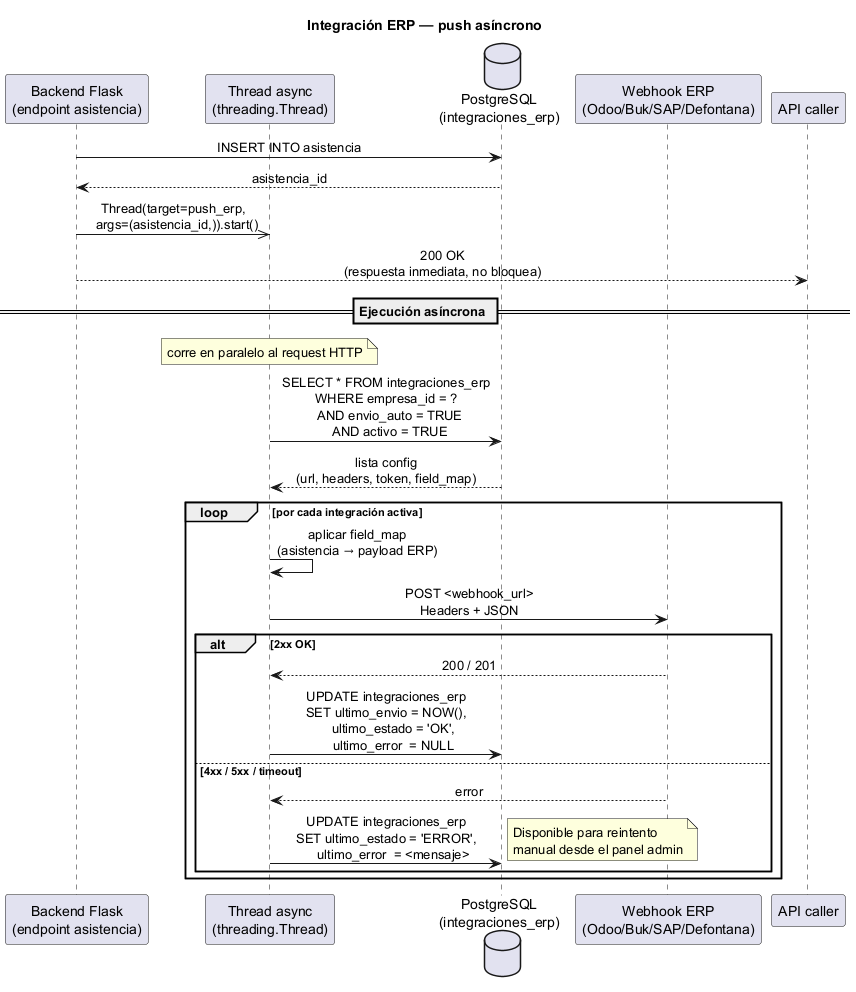
\includegraphics[width=0.95\linewidth]{diagrams/flujo_integracion_erp.png}
  \caption{Diagrama de secuencia de la integración ERP: push asíncrono con field mapping.}
  \label{fig:flujo_erp}
\end{figure}

\subsubsection{Implementación}

\paragraph{Panel web del backend}

Para complementar el backend, se desarrolló un panel web independiente (Next.js 16 \cite{nextjs_docs} con React 19 y TypeScript) cuyo módulo principal es la gestión del dispositivo IoT. Este panel, accesible desde cualquier navegador moderno, permite al administrador:

\begin{itemize}
    \item Visualizar el estado online/offline de cada dispositivo enrolado en tiempo real mediante tarjetas con código de colores, indicador animado (live-dot) y la IP como enlace clickable con la leyenda ``Misma red requerida''.
    \item Generar el PIN de 8 caracteres necesario para enrolar un nuevo ESP32-CAM.
    \item Probar la conectividad activa con un dispositivo específico consultando su endpoint /estado (variable NEXT\_PUBLIC\_DEVICE\_BASE\_URL, por defecto http://192.168.4.1).
    \item Renombrar y eliminar dispositivos registrados.
    \item Acceder a los logs de sincronización generados por el dispositivo.
    \item Acceder a las funcionalidades complementarias de gestión: personas, turnos, asignaciones, asistencias, integración ERP, usuarios y empresas.
\end{itemize}

El estado en tiempo real se obtiene mediante dos mecanismos complementarios. El principal es un hook useDeviceWebSocket que utiliza EventSource para conectarse directamente al endpoint SSE del backend (http://localhost:5000/sse/devices), recibiendo eventos con el id, nombre, IP, estado y timestamp del último heartbeat de cada dispositivo. Como respaldo, un temporizador ejecuta una consulta REST cada 15 segundos (GET /api/dispositivos) para actualizar el estado si la conexión SSE se interrumpe. El estado online se calcula verificando que el campo estado sea 'activo' y que el ultimo\_heartbeat esté dentro de los últimos 5 minutos; si alguna condición falla, el dispositivo se considera offline.

El panel web se comunica con el backend Flask mediante un proxy interno (app/api/\_proxy.ts) que reenvía las peticiones REST a la API, evitando problemas de CORS. La conexión SSE, por su parte, se realiza directamente al backend en el puerto 5000 sin pasar por el proxy, ya que requiere una conexión persistente text/event-stream. La aplicación está protegida por un middleware de autenticación que valida el token JWT y restringe el acceso según el rol del usuario (admin, empleador, trabajador). El frontend se compila con Docker en un build multi-etapa usando output: 'standalone' para producir una imagen optimizada lista para producción.

Para mantener la consistencia visual entre el panel web y la interfaz embebida del ESP32-CAM, las 9 vistas HTML del dispositivo (index.html, register.html, gestion.html, personas.html, turnos.html, asignaciones.html, asistencias.html, logs.html y wifi-setup.html) fueron actualizadas para adoptar la misma paleta oscura, tipografía y sistema de componentes del panel SAS. Se utilizaron variables CSS para la paleta cromática, diseño basado en tarjetas (cards) para la disposición del contenido, y componentes reutilizables para botones, tablas y formularios, logrando que ambas interfaces presenten una experiencia de usuario unificada.

Adicionalmente, el panel web incorpora las siguientes funcionalidades complementarias:

\begin{itemize}
    \item \textbf{Auto-registro de empresas}: La pantalla de inicio de sesión incluye un modo de registro que permite a nuevas empresas crear su cuenta directamente, invocando al endpoint público POST /api/auth/register-company. El formulario solicita nombre de la empresa y datos del administrador de la empresa (nombre, email, contraseña), y al enviarlo crea la organización, el usuario administrador y retorna un token JWT para acceso inmediato.
    \item \textbf{Captura facial por webcam}: El formulario de registro facial en el panel web utiliza la API navigator.mediaDevices.getUserMedia() para capturar fotografías directamente desde la cámara del navegador, eliminando la necesidad de subir archivos desde el sistema de archivos local. La interfaz permite visualizar la vista previa en vivo, capturar, previsualizar y confirmar o repetir la toma, con liberación adecuada del stream al cancelar.
    \item \textbf{Edición de usuarios del sistema}: Los administradores y empleadores pueden editar los datos de los usuarios del sistema (nombre, email, rol, contraseña, estado activo/inactivo) mediante un formulario modal que reutiliza la interfaz de registro en modo edición. Las actualizaciones son parciales: solo se envían los campos modificados.
\end{itemize}

\paragraph{Endpoint de configuración ERP para el ESP32-CAM}

Para que el ESP32-CAM pueda notificar asistencias directamente a los ERP configurados (incluso si el backend central no está disponible), se implementó el endpoint GET /api/dispositivos/erp-config, que retorna la lista de integraciones ERP activas con envío automático habilitado. El ESP32-CAM consulta este endpoint cada hora y almacena la configuración en /erp-config.json, permitiéndole enviar marcaciones a los ERP incluso durante desconexiones parciales.

\paragraph{Contraseñas para autenticación de dispositivos}

Para reforzar la seguridad en la comunicación entre el backend y los ESP32-CAM enrolados, se implementó un sistema de contraseñas de dispositivo que permite al administrador generar, gestionar y verificar credenciales específicas para cada terminal IoT. El flujo contempla cuatro operaciones:

\begin{itemize}
    \item \textbf{Generar contraseña} (POST /api/dispositivos/<id>/generar-password): El administrador solicita una nueva contraseña de 12 caracteres alfanuméricos, generada mediante secrets.choice(). El backend almacena el hash SHA256 de la contraseña, la versión en texto plano (temporal) y marca la contraseña como pendiente (password\_pendiente = TRUE). La respuesta incluye la contraseña en texto plano para que el administrador la proporcione al dispositivo.
    \item \textbf{Verificar contraseña pendiente} (GET /api/dispositivos/check-password): El ESP32-CAM, al iniciar, consulta este endpoint enviando su MAC address como header X-Device-MAC. Si hay una contraseña pendiente, el backend la retorna en texto plano para que el dispositivo la aplique localmente.
    \item \textbf{Confirmar contraseña} (POST /api/dispositivos/confirmar-password): Una vez que el dispositivo ha aplicado la contraseña localmente, confirma al backend, que limpia el texto plano (password\_plain = NULL) y desmarca el estado pendiente. A partir de este momento, solo el hash SHA256 permanece almacenado.
    \item \textbf{Eliminar contraseña} (DELETE /api/dispositivos/<id>/password): El administrador puede eliminar la contraseña de un dispositivo, limpiando el hash y el texto plano.
\end{itemize}

En el panel web, la sección de gestión de dispositivos incorpora botones para generar, regenerar y eliminar contraseñas, así como indicadores visuales del estado de la contraseña (tiene o no tiene, pendiente o confirmada).

\paragraph{Módulo de integración ERP}

El módulo routes/erp.py implementa:

\begin{itemize}
    \item \textbf{enviar\_asistencia\_a\_erps()}: Función central que itera sobre las integraciones ERP activas de una empresa, transforma los datos de la asistencia según el field mapping configurado, y envía una solicitud POST al webhook con los headers personalizados. Registra el resultado (ok o error) en la tabla integraciones\_erp (columnas ultimo\_envio y ultimo\_estado).

    \item \textbf{\_disparar\_erp\_push()}: Wrapper que ejecuta enviar\_asistencia\_a\_erps() en un hilo daemon separado, evitando que la latencia de los ERP externos afecte el tiempo de respuesta al ESP32-CAM. Esta función se invoca automáticamente desde create\_asistencia() y sync\_asistencias() cada vez que se registra una asistencia.

    \item \textbf{CRUD de integraciones}: Endpoints REST para crear, listar y eliminar configuraciones ERP.

    \item \textbf{Test de conectividad} (POST /api/erp/<id>/test): Envía un payload de prueba con datos ficticios al webhook configurado y retorna el código de respuesta y el cuerpo recibido.

    \item \textbf{Envío manual} (POST /api/erp/<id>/enviar): Envía las últimas 200 asistencias de la empresa al ERP seleccionado, útil para cargas históricas o reprocesamiento.

    \item \textbf{Estado de integración} (GET /api/erp/<id>/estado): Retorna el último envío y su estado.
\end{itemize}

\paragraph{Control remoto de dispositivos ESP32}

Se implementaron tres endpoints en routes/dispositivos.py que permiten controlar remotamente los ESP32-CAM enrolados mediante comandos MQTT:

\begin{itemize}
    \item \textbf{Registrar huella} (POST /api/dispositivos/<id>/registrar-huella): Recibe un persona\_id y envía al dispositivo el comando para iniciar el enrolamiento de una huella digital. Verifica que el dispositivo exista, que pertenezca a la empresa del usuario autenticado, y que la persona exista en la misma empresa. Utiliza enviar\_comando\_dispositivo(mac, 'registrar\_huella') para publicar el comando en backend/comando/<MAC>/registrar\_huella. El resultado del enrolamiento se recibe luego por el tópico esp32/huella/resultado/\#.

    \item \textbf{Reiniciar dispositivo} (POST /api/dispositivos/<id>/reiniciar): Envía el comando reiniciar al ESP32-CAM, provocando un reinicio remoto del dispositivo. Útil para recuperar un dispositivo que presenta fallos de conectividad o para aplicar cambios de configuración. Si el cliente MQTT no está disponible, retorna HTTP 503.

    \item \textbf{Reconectar Wi-Fi} (POST /api/dispositivos/<id>/wifi-reconnect): Envía el comando wifi-reconnect para que el dispositivo reinicie su conexión Wi-Fi. Permite recuperar un dispositivo que ha perdido la conectividad sin necesidad de intervención física.
\end{itemize}

Los tres endpoints están protegidos con \textbf{"@requiere\_rol('admin', 'empleador')"} y verifican que el dispositivo pertenezca a la empresa del usuario autenticado. Los comandos se publican en el tópico backend/comando/<MAC>/<comando> mediante la función enviar\_comando\_dispositivo() del módulo mqtt\_handler.py.

\subsubsection{Pruebas}

Se diseñaron las siguientes pruebas para validar el panel web para la gestión del dispositivo y la integración ERP:

\begin{itemize}
    \item \textbf{Prueba de streaming SSE}: Conectar el navegador a http://localhost:5000/sse/devices y verificar que se reciban eventos text/event-stream con datos JSON de los dispositivos. Simular un heartbeat desde un ESP32-CAM y verificar que el evento SSE refleje el cambio a estado activo. Desconectar el dispositivo y verificar que el evento SSE refleje el estado inactivo.

    \item \textbf{Prueba de fallback polling}: Interrumpir la conexión SSE (deteniendo el servidor backend momentáneamente). Verificar que el panel web continúe mostrando el estado de los dispositivos mediante las consultas REST periódicas (cada 15 segundos) y que al restaurar la conexión SSE se retome el streaming.

    \item \textbf{Prueba de indicador visual de dispositivo}: Verificar que cada tarjeta de dispositivo en el panel web muestre: la dirección IP como enlace clickable que abre http://<ip>/ en una nueva pestaña, un indicador animado verde/rojo (live-dot) que refleje el estado online/offline, y la leyenda ``Misma red requerida'' como sugerencia contextual.

    \item \textbf{Prueba de navegación en panel web}: Acceder a las rutas principales del backend (/health, /api/personas, /api/asistencias) sin autenticación y verificar que respondan correctamente (HTTP 200 con acceso público o HTTP 401 cuando se requiera token).

    \item \textbf{Prueba de creación de integración ERP}: Autenticarse como empleador y enviar POST /api/erp con nombre, tipo, webhook URL (usando un servidor de prueba como https://webhook.site) y field mapping. Verificar que la integración se cree con activo = TRUE y envio\_auto = TRUE.

    \item \textbf{Prueba de test de webhook}: Ejecutar POST /api/erp/<id>/test para la integración creada. Verificar que el webhook de prueba reciba un payload JSON con datos ficticios (rut = '11.111.111-1', nombre = "Test Usuario", tipo = "entrada"). Verificar que el estado se actualice en la base de datos.

    \item \textbf{Prueba de envío automático}: Registrar una asistencia real (POST a /api/asistencias) para una persona de la empresa configurada. Verificar que el servidor de prueba del webhook reciba automáticamente el payload con los datos de la asistencia.

    \item \textbf{Prueba de field mapping}: Configurar un ERP con field mapping \{"rut": "employee\_id", "tipo": "event"\}. Registrar una asistencia y verificar que el webhook reciba el payload con los campos renombrados (employee\_id en lugar de rut, event en lugar de tipo).

    \item \textbf{Prueba de envío asíncrono}: Medir el tiempo de respuesta del endpoint POST /api/asistencias cuando hay un ERP configurado cuyo webhook tarda 5 segundos en responder. Verificar que la respuesta al cliente sea inmediata (menor a 200 ms) y que el envío al ERP ocurra en segundo plano.

    \item \textbf{Prueba de tolerancia a fallos ERP}: Configurar un webhook que retorne HTTP 500. Registrar una asistencia y verificar que el sistema no falle; el error debe quedar registrado en ultimo\_estado de la integración y la asistencia debe persistirse correctamente en la base de datos.

    \item \textbf{Prueba de sincronización de configuración ERP al ESP32-CAM}: Simular la consulta GET /api/dispositivos/erp-config desde el ESP32-CAM (con header X-Device-MAC). Verificar que retorne solo las integraciones activas con envío automático de la empresa correspondiente.

    \item \textbf{Prueba de envío manual por lote}: Ejecutar POST /api/erp/<id>/enviar y verificar que se envíen correctamente los registros de asistencia recientes al webhook del ERP.
\end{itemize}

\subsubsection{Refinamientos posteriores}

\begin{itemize}
    \item \textbf{Reasignación de dispositivos entre empresas}: se agregó el endpoint PUT /api/dispositivos/<id>/reasignar, restringido al rol admin, que permite mover un dispositivo ya enrolado de una empresa a otra actualizando su columna empresa\_id. Esto resuelve el caso de dispositivos físicos que cambian de destino (por ejemplo, al reasignar hardware entre sucursales o clientes) sin requerir un nuevo proceso de enrolamiento con PIN.

    \item \textbf{Zona horaria de Chile en la integración ERP}: los timestamps enviados a los webhooks ERP se normalizan a America/Santiago mediante el módulo estándar zoneinfo, con conversión explícita antes de formatear cada fecha\_hora y timestamp del payload. Esto evita ambigüedades cuando el servidor del backend opera en UTC y el sistema ERP de destino espera horarios locales.

    \item \textbf{Soporte de múltiples fotos en el panel web}: el panel de administración construido con Next.js incorpora en la vista de cada persona la visualización de las fotos de referencia asociadas a sus distintos encodings\_faciales, reflejando en la interfaz la capacidad de multi-encoding ya descrita en la Sección 2.3.10. Asimismo, en los despliegues multi-empresa la interfaz incorpora una indicación visual de la empresa a la que pertenece cada registro, relevante para el rol admin, que puede ver datos de más de una organización.
\end{itemize}


%% ============================================================
%% ITERACIÓN 8: Sincronización diferida, logs y cierre del proyecto
%% ============================================================

\subsection{Iteración 8: Sincronización diferida, logs y cierre del proyecto}

Esta iteración integra la sincronización diferida entre el ESP32-CAM y el backend, la capa de auditoría y logs del sistema, y las herramientas de diagnóstico.

\subsubsection{Análisis}

Para que el prototipo sea viable en entornos reales, debe garantizar que ningún dato se pierda durante períodos de desconexión y que todas las operaciones críticas queden registradas para auditoría. Los requisitos identificados son:

\begin{itemize}
    \item \textbf{Sincronización diferida de asistencias}: Los registros de asistencia generados offline (marcados con sincronizado = false) deben enviarse automáticamente al backend cuando se restablezca la conectividad. El proceso debe ser idempotente: si un registro ya existe en el backend, no debe duplicarse.
    \item \textbf{Sincronización diferida de entidades}: Las personas, turnos y asignaciones creados localmente durante el modo offline deben sincronizarse con el backend, resolviendo conflictos de identificadores (IDs locales con prefijo local- versus IDs del backend).
    \item \textbf{Sincronización de configuración ERP}: La configuración de integraciones ERP debe poder descargarse desde el backend para que el ESP32-CAM pueda enviar datos de asistencia directamente a los ERP configurados.
    \item \textbf{Logs de sincronización}: Cada operación de sincronización debe registrarse en la base de datos con el conteo de registros enviados y procesados correctamente, permitiendo auditoría posterior.
    \item \textbf{Logs biométricos}: Todas las operaciones de registro, verificación e identificación facial deben quedar registradas con timestamp, resultado e IP de origen, para cumplimiento normativo.
    \item \textbf{Watchdog de dispositivos}: El backend debe monitorear continuamente el estado de los dispositivos enrolados, detectando aquellos que han dejado de comunicarse y marcándolos como inactivos.
    \item \textbf{Herramientas de diagnóstico}: Se requiere un script de prueba que permita simular asistencias faciales usando fotos almacenadas, facilitando las pruebas del sistema sin necesidad del hardware.
\end{itemize}

\subsubsection{Diseño}

\paragraph{Proceso de sincronización diferida}

El ESP32-CAM ejecuta la sincronización en dos momentos:
\begin{enumerate}
    \item \textbf{Al iniciar}: Si hay conectividad, llama a sincronizarPendientes() que ejecuta en secuencia:
    \begin{itemize}
        \item sincronizarTurnosPendientes(): Envía los turnos con sincronizado = false al backend vía POST, y actualiza sus backend\_id.
        \item sincronizarAsignacionesPendientes(): Similar para asignaciones, dependiendo de que los turnos referenciados ya tengan backend\_id.
        \item sincronizarAsistencias(): Envía un lote de asistencias con sincronizado = false vía POST /api/asistencias/sync.
    \end{itemize}
    \item \textbf{Periódicamente}: Cada 5 minutos (300,000 ms), se ejecuta sincronizarPendientes() en el bucle principal.
\end{enumerate}

Además, el ESP32-CAM consulta GET /api/dispositivos/erp-config cada hora (360,000 ms) para mantener actualizada su configuración local de webhooks ERP.

\begin{figure}[H]
  \centering
  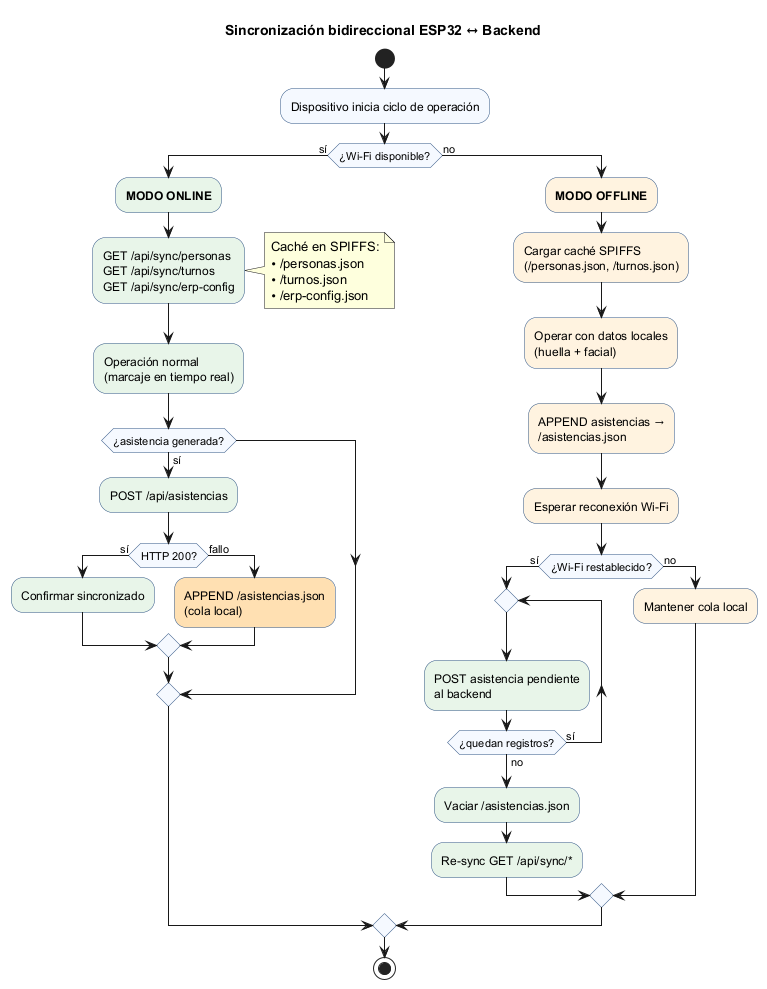
\includegraphics[width=0.95\linewidth]{diagrams/flujo_sincronizacion_bidireccional.png}
  \caption{Diagrama de actividad: sincronización bidireccional entre los modos online y offline del ESP32-CAM.}
  \label{fig:flujo_sync}
\end{figure}

\paragraph{Deduplicación en el backend}

El endpoint POST /api/asistencias/sync implementa una verificación previa a la inserción: para cada registro del lote, consulta si ya existe una asistencia de la misma persona (persona\_id), mismo tipo (entrada/salida), mismo turno\_id y misma fecha (DATE(fecha\_hora) = CURRENT\_DATE). Si existe, omite la inserción. Esta verificación por turno\_id permite que un trabajador registre múltiples asistencias en un mismo día si pertenece a distintos turnos (por ejemplo, jornada diurna y jornada nocturna), sin generar duplicados dentro del mismo turno. Garantiza idempotencia ante reenvíos.

\paragraph{Tablas de auditoría}

\begin{itemize}
    \item sincronizacion\_log: Registra cada operación de sincronización con: dispositivo de origen, cantidad de registros enviados, cantidad procesada correctamente, estado y detalle.
    \item logs\_biometricos: Registra cada operación biométrica con: persona, dispositivo, timestamp, tipo de operación (registro, verificación, identificación), resultado (éxito, fallo, duplicado, no\_encontrado) e IP de origen.
    \item eliminaciones\_biometricas: Registra cada eliminación de datos biométricos con: persona, embedding anterior (cifrado), ruta de la foto eliminada y usuario solicitante.
\end{itemize}

\paragraph{Panel de visualización de logs}

El backend expone dos conjuntos de endpoints para consulta de logs:
\begin{itemize}
    \item GET /api/logs: Lista los registros de sincronización, con filtro por empresa para roles no-admin.
    \item DELETE /api/logs: Permite limpiar los logs (admin limpia todo, empleador limpia los de su empresa).
    \item El ESP32-CAM expone GET /api/logs que retorna el buffer de logs en formato HTML, y /api/logs/clear para limpiarlo.
\end{itemize}

\paragraph{Script de simulación de asistencia facial}

Se desarrolló deteccion.py, un script de línea de comandos que permite probar el flujo de reconocimiento facial sin necesidad del ESP32-CAM. El script escanea las fotos almacenadas localmente para el ambiente de pruebas, presenta un menú interactivo para seleccionar una de ellas, ejecuta el proceso de identificación 1:N contra la base de datos y registra la asistencia correspondiente. Es útil para pruebas de regresión rápida y demostraciones.

\subsubsection{Implementación}

\paragraph{Sincronización en el ESP32-CAM}

Las funciones de sincronización siguen un patrón común:

\begin{enumerate}
    \item Verificar conectividad (isOnline y WiFi.status() == WL\_CONNECTED).
    \item Cargar los datos locales desde LittleFS.
    \item Iterar sobre los registros con sincronizado = false.
    \item Para cada uno, construir el payload JSON y enviarlo al backend vía HTTP POST.
    \item Si el backend responde con éxito (HTTP 200/201), marcar sincronizado = true y actualizar el backend\_id si corresponde.
    \item Persistir los cambios en LittleFS.
\end{enumerate}

Para las personas, además del envío de pendientes, se implementa la descarga completa desde el backend (sincronizarPersonasDesdeBackend()) que sobrescribe el archivo local si no hay registros locales pendientes, manteniendo el ESP32-CAM actualizado con los datos del servidor.

\paragraph{Campo colación en turnos}

Los turnos incorporaron los campos con\_colacion (booleano), colacion\_inicio (TIME) y colacion\_fin (TIME) para modelar el horario de colación de los trabajadores, en cumplimiento del artículo 34 del Código del Trabajo chileno. En la tabla turnos de PostgreSQL se almacenan como TIME (o NULL si con\_colacion = FALSE). Los endpoints CRUD de routes/turnos.py gestionan estos campos: al crear un turno, se envían con\_colacion, colacion\_inicio y colacion\_fin; al actualizar, se usa COALESCE para preservar valores existentes si no se envían. Las consultas GET retornan los horarios como string o null según corresponda. El campo turno\_id se agregó también a la tabla asistencias para asociar cada marcación al turno bajo el cual se registró, permitiendo el cálculo preciso de horas trabajadas descontando la colación.

\paragraph{Sincronización de asistencias por lote}

La función sincronizarAsistencias() en el ESP32-CAM es especialmente relevante porque maneja el caso más frecuente de datos offline: un trabajador marcó entrada y salida durante el día sin conexión. La función:

\begin{enumerate}
    \item Carga asistencias.json y filtra las que tengan sincronizado = false.
    \item Construye un JSON con estructura \{"registros": [...]\}.
    \item Lo envía a POST /api/asistencias/sync.
    \item Si el backend retorna HTTP 200, marca todos los registros enviados como sincronizados.
\end{enumerate}

\paragraph{Sincronización en el backend}

El endpoint POST /api/asistencias/sync en routes/asistencias.py recibe el lote e itera sobre cada registro, aplicando la verificación de duplicados y realizando la inserción. También dispara el envío a ERP para cada asistencia nueva.

\paragraph{Watchdog y ping activo de dispositivos}

La detección de desconexión de dispositivos se implementó con tres capas complementarias:

\begin{enumerate}
    \item \textbf{LWT (instantáneo)}: Al conectarse al broker MQTT, el ESP32-CAM configura un mensaje Last Will en esp32/lwt/<MAC>. Si el dispositivo se desconecta abruptamente, el broker publica automáticamente el LWT y el backend marca el dispositivo como inactivo de inmediato.
    \item \textbf{Ping activo (device\_pinger)}: Un hilo separado publica periódicamente (cada 30 segundos) un mensaje en el tópico esp32/ping/<MAC>. El ESP32-CAM, al recibirlo, responde publicando un heartbeat con el campo "pong": true. Si el backend no recibe respuesta dentro de 60 segundos, marca el dispositivo como inactivo. Este mecanismo funciona incluso si el mensaje LWT no fue entregado.
    \item \textbf{Watchdog pasivo (device\_watchdog)}: Un hilo ejecutado cada 60 segundos realiza un barrido inicial al arrancar el backend (todos los dispositivos se marcan inactivo) y luego verifica periódicamente qué dispositivos no han enviado heartbeat en más de 90 segundos, marcándolos como inactivos.
\end{enumerate}

Esta arquitectura de tres capas asegura que ninguna desconexión pase desapercibida: el LWT atrapa las desconexiones abruptas detectadas por el broker; el ping activo detecta silencios de red donde el LWT no alcanza a publicarse; y el watchdog pasivo actúa como respaldo final para cualquier caso no cubierto por las capas anteriores.

\paragraph{Herramienta de simulación facial}

Como complemento durante el desarrollo se implementó deteccion.py, un script de línea de comandos que permitió probar el flujo de reconocimiento facial sin necesidad del ESP32-CAM. El script se conectaba directamente a PostgreSQL, ejecutaba DeepFace (Facenet + detector configurable + anti-spoofing) sobre imágenes almacenadas localmente para el ambiente de pruebas, y registraba asistencias de prueba en la base de datos. En las etapas finales del proyecto, esta funcionalidad de simulación fue absorbida por la suite de pruebas automatizadas (con mocks de DeepFace, OpenCV y PostgreSQL en Docker), que ofrece mayor repetibilidad y cobertura sin dependencia del sistema de archivos local.

\paragraph{Flujo operacional consolidado}
\label{sec:flujo_operacional_consolidado}

Con todos los componentes del sistema ya construidos (enrolamiento por PIN, reconocimiento biométrico, almacenamiento offline, sincronización diferida e integración ERP), la Fig.~\ref{fig:flujo_operacional} consolida el camino completo que sigue una marcación, cubriendo tanto el caso con conexión a internet como el caso sin ella, tal como quedó implementado al cierre del proyecto.

El flujo comienza cuando el sensor PIR detecta presencia frente al dispositivo y se ejecuta la captura biométrica (huella mediante el AS608 o rostro mediante la cámara OV2640). A partir de ahí, el firmware evalúa isCloudReady(): si el dispositivo está conectado a internet y enrolado, la marcación se envía de inmediato al backend por HTTP (POST /api/facial/identificar para rostro, o POST /api/asistencias para huella). Si cualquiera de esas dos condiciones falla, la marcación se guarda localmente en asistencias.json (LittleFS) con la marca sincronizado=false, se muestra el resultado en el panel embebido sin esperar respuesta del servidor, y el dispositivo queda a la espera de que la conexión se restablezca para ejecutar sincronizarPendientes(), que vacía la cola completa hacia el backend.

Ambos caminos, el envío inmediato y la sincronización diferida, terminan convergiendo en el mismo punto: el backend valida la huella o el rostro contra los registros almacenados (encodings\_faciales o el identificador de huella) y persiste el resultado en la tabla asistencias de PostgreSQL. Si la identificación es exitosa, el backend responde 200 OK, dispara en un hilo aparte el envío hacia los sistemas ERP configurados, y el firmware ejecuta flashExito(), que hace parpadear el LED verde del dispositivo dos veces. Si no hay coincidencia o la imagen no cumple el filtro de calidad, el backend responde con un código de error (404 o 400) y la operación queda registrada en logs\_biometricos para su auditoría posterior; en este caso el firmware invoca flashError(), una función que existe en el código como punto de extensión para una señal de error distinta, pero que actualmente no tiene ninguna acción implementada.

\begin{figure}[H]
    \centering
    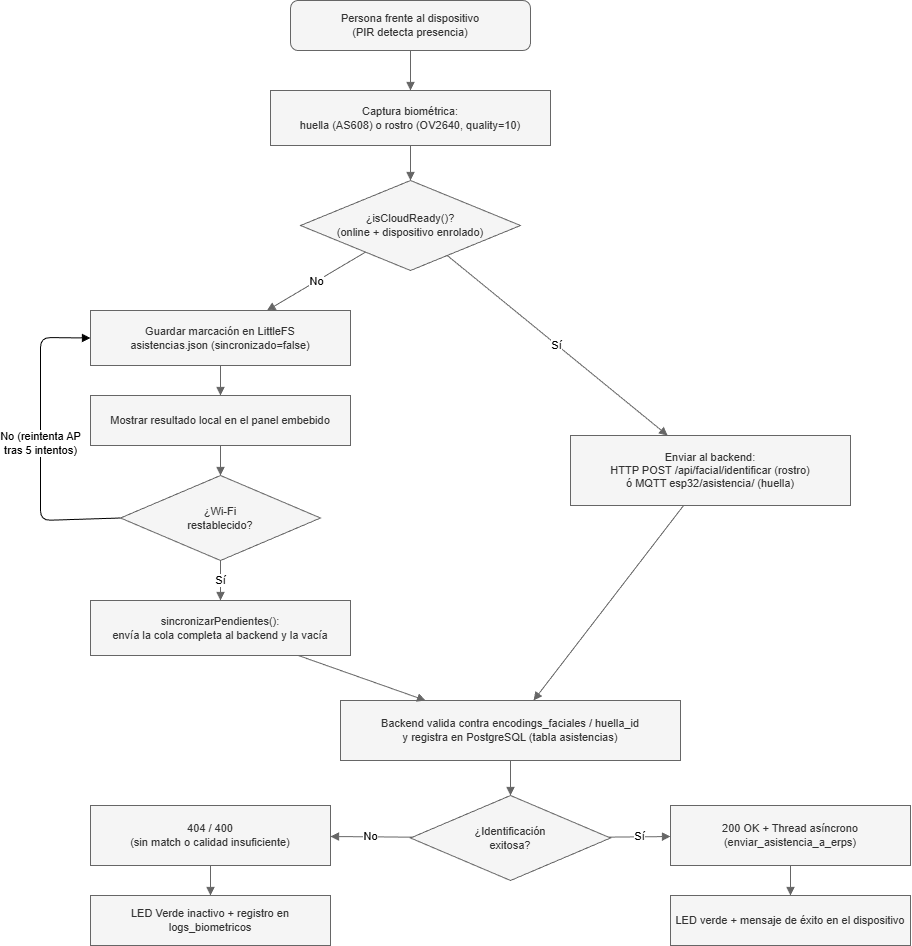
\includegraphics[width=.85\linewidth]{Imagenes/flujo_operacional_asistencia.png}
    \caption{Flujo operacional consolidado para el registro de asistencia.}
    \label{fig:flujo_operacional}
\end{figure}

\subsubsection{Pruebas}
\label{sec:pruebas_unitarias_automatizadas}

Se diseñaron las siguientes pruebas para validar la sincronización diferida, los logs y la integración final:

\begin{itemize}
    \item \textbf{Prueba de sincronización de asistencias offline}: Desconectar el ESP32-CAM de la red, registrar 5 marcaciones de entrada/salida para 2 personas diferentes, reconectar y ejecutar sincronización. Verificar que los 5 registros aparezcan en la base de datos del backend y que el archivo asistencias.json local los marque como sincronizados.

    \item \textbf{Prueba de idempotencia de sincronización}: Tras una sincronización exitosa, ejecutar nuevamente la sincronización sin nuevos registros. Verificar que no se inserten registros duplicados en el backend.

    \item \textbf{Prueba de sincronización de personas creadas offline}: Desconectar el dispositivo, registrar una nueva persona (con huella y datos), reconectar y sincronizar. Verificar que la persona aparezca en el backend con un ID definitivo (no local-).

    \item \textbf{Prueba de sincronización de turnos y asignaciones}: Desconectar el dispositivo, crear un turno y asignarlo a una persona existente, reconectar y sincronizar. Verificar que el turno y la asignación se repliquen en el backend y que los backend\_id locales se actualicen correctamente.

    \item \textbf{Prueba de persistencia tras corte de energía}: Durante una sincronización en curso, cortar la alimentación del ESP32-CAM. Al reiniciar, verificar que los archivos JSON no estén corruptos y que los registros con sincronizado = false sigan estando disponibles para una nueva sincronización.

    \item \textbf{Prueba de duplicados por turno}: Registrar dos asistencias con la misma persona, tipo, turno y fecha. Verificar que el sistema rechace la segunda inserción por duplicado. Registrar asistencias con diferentes turno\_id para un mismo día y verificar que ambas se registren sin conflictos.

    \item \textbf{Prueba de colación en turnos}: Crear un turno con colación habilitada (con\_colación = true) especificando horario de colación. Verificar que los campos colacion\_inicio y colacion\_fin se almacenen correctamente como TIME en la base de datos. Crear un turno sin colación y verificar que ambos campos sean NULL.

    \item \textbf{Prueba de logs de sincronización}: Ejecutar 3 sincronizaciones con diferentes cantidades de registros. Verificar que en la tabla sincronizacion\_log del backend aparezcan 3 entradas con los conteos correctos de registros enviados y procesados.

    \item \textbf{Prueba de logs biométricos}: Realizar operaciones de registro facial, identificación exitosa, identificación fallida y verificación. Verificar que cada operación genere una entrada en logs\_biometricos con el tipo de operación y resultado correctos.

    \item \textbf{Prueba de watchdog}: Iniciar el backend, verificar que todos los dispositivos se marquen como inactivos. Conectar un ESP32-CAM, verificar que tras el primer heartbeat cambie a activo. Desconectar el ESP32-CAM y verificar que tras 90 segundos el watchdog lo marque como inactivo.

    \item \textbf{Prueba de ping activo}: Conectar un ESP32-CAM, verificar que el backend publique pings en esp32/ping/<MAC> y que el dispositivo responda. Detener el ESP32-CAM (corte de red) y verificar que el ping activo marque el dispositivo como inactivo antes de que el watchdog de 90 segundos actúe (tiempo de espera de 60 segundos).

    \item \textbf{Prueba de simulación facial automatizada}: Utilizar la suite de pruebas test\_routes\_facial.py y el emulador test\_identificacion\_facial.py para simular el flujo completo de identificación 1:N con imágenes sintéticas generadas en memoria, cubriendo casos de coincidencia exitosa, rostro no registrado y calidad insuficiente de imagen.

    \item \textbf{Prueba de flujo completo punta a punta}: Ejecutar el flujo completo: registrar persona con huella y rostro en el ESP32-CAM $\rightarrow$ sincronizar con backend $\rightarrow$ verificar que la persona aparezca en el panel web $\rightarrow$ marcar asistencia por huella offline $\rightarrow$ reconectar y sincronizar $\rightarrow$ verificar que la asistencia aparezca en el panel web y se envíe al ERP de prueba.
\end{itemize}

\paragraph{Pruebas automatizadas}

Además de las pruebas funcionales descritas, se implementó una suite de más de 590 pruebas automatizadas para el backend y el firmware, utilizando pytest con PostgreSQL en Docker y mocks para DeepFace, OpenCV y MQTT. La suite se organiza en 35 archivos de prueba y alcanza una cobertura de código del 98\% sobre el código de producción del backend, sin fallos en ninguna de las pruebas (ver Anexo D para el detalle de casos y la evolución de la cobertura por módulo). La integración con los ERP externos se valida en dos niveles: por un lado, las pruebas de la suite automatizada cubren la creación, edición y prueba de webhooks de una integración ERP, simulando la respuesta del servidor externo. Por otro lado, dentro del subdirectorio ERPSIMULATORS/ se construyeron tres simuladores independientes (mock\_odoo.py, mock\_defontana.py y mock\_buk.py), cada uno levantando un pequeño servidor Flask que reproduce los endpoints reales de autenticación, consulta de empleados e inyección de marcaciones de su respectivo ERP comercial, según la documentación pública de cada proveedor. El script test\_erp\_mocks.py se ejecuta por separado, con los tres simuladores corriendo: envía una marcación con el formato que genera el sistema hacia cada uno de los tres mocks y verifica que el field mapping configurado para cada ERP transforme correctamente los datos y que cada simulador responda como lo haría el sistema real, imprimiendo un reporte de éxito o falla por caso. Esta validación manual complementa, sin sustituir, a las pruebas automatizadas de pytest.

Las pruebas cubren los flujos de todas las iteraciones: inicialización de la aplicación, esquema de base de datos, cifrado de embeddings, servicio de correo electrónico (con mock de SMTP), handlers MQTT, autenticación JWT con roles jerárquicos y flujo multi-empresa, endpoints faciales, CRUD de personas/turnos/asignaciones/asistencias, verificación de dispositivos, integraciones ERP con tolerancia a fallos de conexión y timeout, enrolamiento de dispositivos mediante PIN, sincronización offline, y logs de auditoría. Entre los módulos con mayor cobertura destacan el cifrado de embeddings (100\%), el servicio de correo (100\%), la gestión de turnos (100\%), la base de datos (99\%) y el módulo de asignaciones (96\%). El detalle completo de los casos de prueba se incluye en el Anexo D, que además resume los resultados obtenidos al ejecutar la suite completa.

\subsubsection{Refinamientos posteriores}

\begin{itemize}
    \item \textbf{Limpieza de datos al eliminar una persona}: el endpoint de eliminación distingue dos comportamientos según el rol de quien lo invoca. Un administrador ejecuta una limpieza completa de datos biométricos y sensibles: anonimiza el RUT, el correo y el identificador de huella, elimina los encodings\_faciales y los consentimientos asociados, borra la foto de previsualización del disco y marca a la persona como inactiva, conservando únicamente su historial de asistencias. Un empleador, en cambio, solo puede marcar a la persona como inactiva, sin acceso a la limpieza de datos biométricos, reservada al rol con mayor privilegio.

    \item \textbf{Filtro activo = true en los listados}: todas las consultas de lectura sobre personas (y entidades equivalentes) incorporan la condición WHERE activo = true, de modo que los registros eliminados mediante soft-delete dejan de aparecer en listados y búsquedas sin perder su información histórica en la base de datos, requisito necesario para mantener la integridad de los reportes de asistencia ya generados.
\end{itemize}


\section{Mecanismos de seguridad}

Esta sección consolida los mecanismos de seguridad implementados a lo largo de las distintas iteraciones, descritos en su momento dentro del desarrollo de cada una (Secciones 4.2.3 a 4.2.5), agrupándolos por capa: autenticación y control de acceso, enrolamiento de dispositivos, y protección de datos biométricos.

\subsection{Autenticación y control de acceso}

El backend define tres decoradores de autenticación en routes/auth.py, aplicados según el tipo de cliente que consume cada endpoint:

\begin{itemize}
    \item @token\_required: exige un header Authorization: Bearer <token> con un JWT firmado con el algoritmo HS256 y una clave secreta (JWT\_SECRET, configurable por variable de entorno). El token incluye user\_id, empresa\_id, rol y, opcionalmente, persona\_id, con una expiración de 24 horas. Si el token falta, está expirado o es inválido, el endpoint responde con HTTP 401.

    \item @requiere\_rol(*roles): envuelve a @token\_required y además exige que request.user\_rol esté dentro de los roles permitidos (admin, empleador o trabajador), respondiendo HTTP 403 en caso contrario. Implementa así un control de acceso jerárquico basado en roles sobre los mismos endpoints autenticados.

    \item @token\_opcional: permite que un mismo endpoint sea consumido tanto por un cliente web autenticado con JWT como por un dispositivo ESP32-CAM identificado mediante el header X-Device-MAC. Si no hay JWT, el decorador busca la MAC recibida entre los dispositivos ya enrolados y, de encontrarla, expone request.dispositivo\_id y request.empresa\_id para el resto del endpoint. Como se detalla en la Sección 4.2.5, este decorador ya no crea dispositivos nuevos automáticamente: solo vincula los que ya pasaron por el flujo de enrolamiento con PIN.

    \item @requiere\_dispositivo\_enrolado: complementa a @token\_opcional en endpoints biométricos sensibles (por ejemplo, /api/facial/registrar), verificando explícitamente que el dispositivo de la petición tenga enrolado = TRUE en la base de datos antes de continuar, y respondiendo HTTP 403 en caso contrario.
\end{itemize}

Las contraseñas de los usuarios del panel web nunca se almacenan en texto plano: se procesan con bcrypt \cite{bcrypt_pypi} (función hashpw con sal generada por gensalt()) tanto al crear una cuenta como al cambiar la contraseña, y la verificación en el login usa bcrypt.checkpw para comparar contra el hash almacenado.

\subsection{Enrolamiento seguro de dispositivos}

Un dispositivo ESP32-CAM no puede operar contra el backend simplemente conectándose a la red: debe pasar por un flujo de enrolamiento explícito basado en un PIN de un solo uso. Un administrador o empleador solicita POST /api/auth/dispositivos/generar-pin, que crea en la base de datos un registro en dispositivos con enrolado = FALSE y un código aleatorio de 8 caracteres alfanuméricos (generado con el módulo secrets, criptográficamente seguro). El dispositivo, desde su panel de configuración Wi-Fi, envía ese PIN junto con su dirección MAC al backend; si el PIN es válido y no fue usado antes, el dispositivo queda marcado como enrolado = TRUE y asociado a la MAC y a la empresa que generó el PIN. Un PIN ya consumido no puede reutilizarse (HTTP 409).

En el firmware, la función isCloudReady() (Sección 4.2.1) actúa como una verificación de doble factor antes de cualquier operación dependiente del backend: exige tanto conectividad de red (isOnline) como enrolamiento confirmado (estaEnrolado), evitando que un dispositivo conectado pero no autorizado, o autorizado pero sin red, ejecute operaciones que comprometerían la consistencia del sistema.

\subsection{Protección de datos biométricos}

Los embeddings faciales generados por DeepFace se cifran antes de almacenarse en la base de datos mediante Fernet (AES-128 en modo CBC con autenticación HMAC-SHA256), de la librería cryptography de Python. La clave de cifrado no se almacena directamente: se deriva aplicando SHA-256 a una variable de entorno (BIOMETRIC\_KEY) y codificando el resultado en base64 URL-safe, tal como lo exige la API de Fernet:

\begin{verbatim}
def _derivar_fernet_key() -> bytes:
    digest = hashlib.sha256(BIOMETRIC_KEY.encode("utf-8")).digest()
    return base64.urlsafe_b64encode(digest)
\end{verbatim}

De esta forma, ni el embedding ni la clave de cifrado quedan expuestos en texto plano en la base de datos: un acceso no autorizado a las tablas encodings\_faciales solo expone valores cifrados, mientras la clave reside exclusivamente en la configuración del entorno de ejecución del backend.

\section{Arquitectura de tiempo real (SSE)}

El panel web necesita reflejar, sin recargar la página, el estado de conexión de cada ESP32-CAM y el progreso del enrolamiento de huellas. Esta sección consolida cómo se implementó esa capa de tiempo real, descrita parcialmente al introducirse en las iteraciones 3 y 7 (Secciones 4.2.3 y 4.2.5).

\subsection{Endpoints de streaming}

El backend expone dos endpoints SSE (Server-Sent Events) implementados en app.py con el patrón estándar de Flask para streaming: una función generadora que produce eventos en formato text/event-stream, devuelta mediante Response(stream\_with\_context(generate()), mimetype='text/event-stream').

\begin{itemize}
    \item GET /sse/devices: difunde, a todos los clientes conectados, los cambios de estado de los dispositivos (heartbeat recibido, LWT disparado, ping sin respuesta), mediante la función broadcast\_device\_update().
    \item GET /sse/huellas: difunde el resultado del enrolamiento de huellas recibido por MQTT en esp32/huella/resultado/\#, mediante broadcast\_huella\_update(), permitiendo que el panel muestre en vivo el progreso del registro biométrico.
\end{itemize}

Se optó por SSE porque el caso de uso es unidireccional (servidor a cliente) y se consume en el navegador con la API nativa EventSource, sin depender de librerías adicionales en el frontend ni de un protocolo de negociación propio como el de WebSockets.

\subsection{Tres capas de detección de desconexión}

Determinar si un ESP32-CAM sigue conectado es más complejo que solo esperar sus heartbeats, porque una caída de red puede impedir que el dispositivo avise que se desconectó. El backend combina tres mecanismos complementarios, implementados en mqtt\_handler.py:

\begin{enumerate}
    \item \textbf{LWT (Last Will and Testament)}: al conectarse al broker MQTT, el ESP32-CAM registra un mensaje LWT en esp32/lwt/<MAC>. Si la conexión TCP se rompe de forma anómala (corte de energía, pérdida abrupta de señal), el propio broker Mosquitto publica ese mensaje automáticamente, sin que el backend tenga que esperar ningún timeout. Es la capa más rápida, pero depende de que el broker detecte la caída de la conexión subyacente.

    \item \textbf{Ping activo (device\_pinger)}: un hilo en segundo plano publica, cada 30 segundos, un mensaje en esp32/ping/<MAC> para cada dispositivo enrolado. El ESP32-CAM responde con un heartbeat normal al recibirlo. Si un dispositivo no responde dentro de la ventana definida por HEARTBEAT\_TIMEOUT (60 segundos), el pinger lo marca como inactivo directamente, sin esperar al watchdog. Esta capa cubre los casos en que el LWT no llega a publicarse (por ejemplo, si el broker tampoco detecta la caída).

    \item \textbf{Watchdog pasivo (device\_watchdog)}: un segundo hilo revisa cada 60 segundos la antigüedad del último heartbeat de cada dispositivo y marca como inactivos a los que superan los 60 segundos sin responder. Actúa como respaldo final, independiente del pinger, y además ejecuta un barrido inicial al arrancar el backend que marca a todos los dispositivos como inactivos hasta recibir su primer heartbeat.
\end{enumerate}

Cada vez que cualquiera de estas tres capas cambia el estado de un dispositivo en la base de datos, invoca broadcast\_device\_update(), que propaga el cambio de inmediato a los clientes SSE conectados.

\subsection{Consumo en el frontend}

En el panel web (Next.js), un hook personalizado se conecta directamente al endpoint /sse/devices mediante EventSource, actualizando en memoria el estado, IP y último heartbeat de cada dispositivo a medida que llegan eventos, sin necesidad de refrescar la página ni de mantener una conexión WebSocket. Como mecanismo de respaldo ante una eventual interrupción de la conexión SSE, el frontend además consulta periódicamente GET /api/dispositivos por REST, de modo que el estado mostrado no depende exclusivamente del canal de streaming.

\section{Prototipo final}
\label{sec:prototipo_final}

Esta sección presenta el resultado físico del proceso de desarrollo descrito en las ocho iteraciones anteriores, mostrando el dispositivo ESP32-CAM ensamblado junto con sus componentes periféricos (cámara OV2640, lector de huellas AS608 y sensor PIR), así como el panel web resultante.

%% Reemplazar por las fotografías reales del prototipo final.
%% Se recomienda incluir: (1) vista general del dispositivo ensamblado,
%% (2) detalle de conexiones/componentes, (3) dispositivo en su carcasa/montaje final,
%% (4) captura del panel web administrativo en funcionamiento.

\begin{figure}[H]
  \centering
  \includegraphics[width=0.75\linewidth]{Imagenes/prototipo_final_1.jpg}
  \caption{Vista general del prototipo final ensamblado.}
  \label{fig:prototipo_final_1}
\end{figure}

\begin{figure}[H]
  \centering
  \includegraphics[width=0.75\linewidth]{Imagenes/prototipo_final_2.jpg}
  \caption{Detalle de los componentes del prototipo: cámara OV2640, lector de huellas AS608 y sensor PIR.}
  \label{fig:prototipo_final_2}
\end{figure}

\begin{figure}[H]
  \centering
  \includegraphics[width=0.75\linewidth]{Imagenes/prototipo_final_3.jpg}
  \caption{Prototipo final montado en su carcasa definitiva.}
  \label{fig:prototipo_final_3}
\end{figure}

\begin{figure}[H]
  \centering
  \includegraphics[width=0.9\linewidth]{Imagenes/prototipo_final_4.jpg}
  \caption{Panel web administrativo en funcionamiento durante una prueba de campo.}
  \label{fig:prototipo_final_4}
\end{figure}

%% ============================================================
\section{Resumen del capítulo}
El capítulo 4 presenta el desarrollo completo del prototipo a lo largo de ocho iteraciones, siguiendo la metodología de prototipado evolutivo incremental. Se documenta la integración del hardware (ESP32-CAM, lector AS608, sensor PIR, cámara OV2640), la implementación del almacenamiento local con LittleFS y JSON, el desarrollo del backend con Flask y PostgreSQL (14 tablas con soporte multi-tenant), la comunicación mediante HTTP y MQTT, el reconocimiento facial con DeepFace (modelo Facenet, detector configurable MTCNN/RetinaFace y anti-spoofing), el cifrado de embeddings biométricos con Fernet, la autenticación JWT con roles jerárquicos, el enrolamiento seguro de dispositivos mediante PIN, el sistema antifraude multicapa (PIR + flash PWM + anti-spoofing + cooldown), el panel web para la gestión del dispositivo con streaming SSE de estado en tiempo real, la integración con ERP externos vía webhooks con field mapping, los mecanismos de sincronización diferida con logs de auditoría, y la detección de desconexión mediante un sistema de tres capas (LWT, ping activo y watchdog pasivo).

Cada iteración incluyó su respectivo análisis de requisitos, diseño de la solución, implementación detallada y un plan de pruebas de integración para validar el correcto funcionamiento de los componentes desarrollados. Adicionalmente, se documenta la suite de 591 pruebas unitarias automatizadas con pytest, que alcanzó una cobertura de código del 98\% sobre las 3.382 líneas de producción del backend, incluyendo pruebas de caja negra sobre los endpoints de la API REST y verificación exhaustiva de todos los caminos de error.

El Anexo C presenta, mediante diagramas de actividades, las principales funcionalidades implementadas en el sistema: el enrolamiento de dispositivos (Figura~\ref{fig:flujo_enrolamiento_dispositivo}), el registro de personas y captura biométrica (Figura~\ref{fig:flujo_registro_personas}), la gestión de turnos y su asignación (Figura~\ref{fig:flujo_gestion_turnos}), la sincronización diferida de asistencias pendientes (Figura~\ref{fig:flujo_sincronizacion_pendientes}) y el panel web administrativo (Figura~\ref{fig:flujo_panel_administrativo}).